% Options for packages loaded elsewhere
\PassOptionsToPackage{unicode}{hyperref}
\PassOptionsToPackage{hyphens}{url}
%
\documentclass[
]{book}
\usepackage{amsmath,amssymb}
\usepackage{iftex}
\ifPDFTeX
  \usepackage[T1]{fontenc}
  \usepackage[utf8]{inputenc}
  \usepackage{textcomp} % provide euro and other symbols
\else % if luatex or xetex
  \usepackage{unicode-math} % this also loads fontspec
  \defaultfontfeatures{Scale=MatchLowercase}
  \defaultfontfeatures[\rmfamily]{Ligatures=TeX,Scale=1}
\fi
\usepackage{lmodern}
\ifPDFTeX\else
  % xetex/luatex font selection
\fi
% Use upquote if available, for straight quotes in verbatim environments
\IfFileExists{upquote.sty}{\usepackage{upquote}}{}
\IfFileExists{microtype.sty}{% use microtype if available
  \usepackage[]{microtype}
  \UseMicrotypeSet[protrusion]{basicmath} % disable protrusion for tt fonts
}{}
\makeatletter
\@ifundefined{KOMAClassName}{% if non-KOMA class
  \IfFileExists{parskip.sty}{%
    \usepackage{parskip}
  }{% else
    \setlength{\parindent}{0pt}
    \setlength{\parskip}{6pt plus 2pt minus 1pt}}
}{% if KOMA class
  \KOMAoptions{parskip=half}}
\makeatother
\usepackage{xcolor}
\usepackage{color}
\usepackage{fancyvrb}
\newcommand{\VerbBar}{|}
\newcommand{\VERB}{\Verb[commandchars=\\\{\}]}
\DefineVerbatimEnvironment{Highlighting}{Verbatim}{commandchars=\\\{\}}
% Add ',fontsize=\small' for more characters per line
\usepackage{framed}
\definecolor{shadecolor}{RGB}{248,248,248}
\newenvironment{Shaded}{\begin{snugshade}}{\end{snugshade}}
\newcommand{\AlertTok}[1]{\textcolor[rgb]{0.94,0.16,0.16}{#1}}
\newcommand{\AnnotationTok}[1]{\textcolor[rgb]{0.56,0.35,0.01}{\textbf{\textit{#1}}}}
\newcommand{\AttributeTok}[1]{\textcolor[rgb]{0.13,0.29,0.53}{#1}}
\newcommand{\BaseNTok}[1]{\textcolor[rgb]{0.00,0.00,0.81}{#1}}
\newcommand{\BuiltInTok}[1]{#1}
\newcommand{\CharTok}[1]{\textcolor[rgb]{0.31,0.60,0.02}{#1}}
\newcommand{\CommentTok}[1]{\textcolor[rgb]{0.56,0.35,0.01}{\textit{#1}}}
\newcommand{\CommentVarTok}[1]{\textcolor[rgb]{0.56,0.35,0.01}{\textbf{\textit{#1}}}}
\newcommand{\ConstantTok}[1]{\textcolor[rgb]{0.56,0.35,0.01}{#1}}
\newcommand{\ControlFlowTok}[1]{\textcolor[rgb]{0.13,0.29,0.53}{\textbf{#1}}}
\newcommand{\DataTypeTok}[1]{\textcolor[rgb]{0.13,0.29,0.53}{#1}}
\newcommand{\DecValTok}[1]{\textcolor[rgb]{0.00,0.00,0.81}{#1}}
\newcommand{\DocumentationTok}[1]{\textcolor[rgb]{0.56,0.35,0.01}{\textbf{\textit{#1}}}}
\newcommand{\ErrorTok}[1]{\textcolor[rgb]{0.64,0.00,0.00}{\textbf{#1}}}
\newcommand{\ExtensionTok}[1]{#1}
\newcommand{\FloatTok}[1]{\textcolor[rgb]{0.00,0.00,0.81}{#1}}
\newcommand{\FunctionTok}[1]{\textcolor[rgb]{0.13,0.29,0.53}{\textbf{#1}}}
\newcommand{\ImportTok}[1]{#1}
\newcommand{\InformationTok}[1]{\textcolor[rgb]{0.56,0.35,0.01}{\textbf{\textit{#1}}}}
\newcommand{\KeywordTok}[1]{\textcolor[rgb]{0.13,0.29,0.53}{\textbf{#1}}}
\newcommand{\NormalTok}[1]{#1}
\newcommand{\OperatorTok}[1]{\textcolor[rgb]{0.81,0.36,0.00}{\textbf{#1}}}
\newcommand{\OtherTok}[1]{\textcolor[rgb]{0.56,0.35,0.01}{#1}}
\newcommand{\PreprocessorTok}[1]{\textcolor[rgb]{0.56,0.35,0.01}{\textit{#1}}}
\newcommand{\RegionMarkerTok}[1]{#1}
\newcommand{\SpecialCharTok}[1]{\textcolor[rgb]{0.81,0.36,0.00}{\textbf{#1}}}
\newcommand{\SpecialStringTok}[1]{\textcolor[rgb]{0.31,0.60,0.02}{#1}}
\newcommand{\StringTok}[1]{\textcolor[rgb]{0.31,0.60,0.02}{#1}}
\newcommand{\VariableTok}[1]{\textcolor[rgb]{0.00,0.00,0.00}{#1}}
\newcommand{\VerbatimStringTok}[1]{\textcolor[rgb]{0.31,0.60,0.02}{#1}}
\newcommand{\WarningTok}[1]{\textcolor[rgb]{0.56,0.35,0.01}{\textbf{\textit{#1}}}}
\usepackage{longtable,booktabs,array}
\usepackage{calc} % for calculating minipage widths
% Correct order of tables after \paragraph or \subparagraph
\usepackage{etoolbox}
\makeatletter
\patchcmd\longtable{\par}{\if@noskipsec\mbox{}\fi\par}{}{}
\makeatother
% Allow footnotes in longtable head/foot
\IfFileExists{footnotehyper.sty}{\usepackage{footnotehyper}}{\usepackage{footnote}}
\makesavenoteenv{longtable}
\usepackage{graphicx}
\makeatletter
\def\maxwidth{\ifdim\Gin@nat@width>\linewidth\linewidth\else\Gin@nat@width\fi}
\def\maxheight{\ifdim\Gin@nat@height>\textheight\textheight\else\Gin@nat@height\fi}
\makeatother
% Scale images if necessary, so that they will not overflow the page
% margins by default, and it is still possible to overwrite the defaults
% using explicit options in \includegraphics[width, height, ...]{}
\setkeys{Gin}{width=\maxwidth,height=\maxheight,keepaspectratio}
% Set default figure placement to htbp
\makeatletter
\def\fps@figure{htbp}
\makeatother
\setlength{\emergencystretch}{3em} % prevent overfull lines
\providecommand{\tightlist}{%
  \setlength{\itemsep}{0pt}\setlength{\parskip}{0pt}}
\setcounter{secnumdepth}{5}
\usepackage{booktabs}
\usepackage{amsthm}
\DeclareMathOperator*{\argmin}{argmin}
\usepackage{titling, amsmath, amsbsy}
\pretitle{\begin{center} \includegraphics[width=2in,height=2in]{figs/UoN_Primary_Logo_RGB.png}\LARGE\\}
\posttitle{\end{center}}
\usepackage{booktabs}
\usepackage{longtable}
\usepackage{array}
\usepackage{multirow}
\usepackage{wrapfig}
\usepackage{float}
\usepackage{colortbl}
\usepackage{pdflscape}
\usepackage{tabu}
\usepackage{threeparttable}
\usepackage{threeparttablex}
\usepackage[normalem]{ulem}
\usepackage{makecell}
\usepackage{xcolor}
\ifLuaTeX
  \usepackage{selnolig}  % disable illegal ligatures
\fi
\usepackage[]{natbib}
\bibliographystyle{apalike}
\usepackage{bookmark}
\IfFileExists{xurl.sty}{\usepackage{xurl}}{} % add URL line breaks if available
\urlstyle{same}
\hypersetup{
  pdftitle={Multivariate Statistics},
  pdfauthor={Prof.~Richard Wilkinson},
  hidelinks,
  pdfcreator={LaTeX via pandoc}}

\title{Multivariate Statistics}
\author{Prof.~Richard Wilkinson}
\date{Spring 2025}

\usepackage{amsthm}
\newtheorem{theorem}{Theorem}[chapter]
\newtheorem{lemma}{Lemma}[chapter]
\newtheorem{corollary}{Corollary}[chapter]
\newtheorem{proposition}{Proposition}[chapter]
\newtheorem{conjecture}{Conjecture}[chapter]
\theoremstyle{definition}
\newtheorem{definition}{Definition}[chapter]
\theoremstyle{definition}
\newtheorem{example}{Example}[chapter]
\theoremstyle{definition}
\newtheorem{exercise}{Exercise}[chapter]
\theoremstyle{definition}
\newtheorem{hypothesis}{Hypothesis}[chapter]
\theoremstyle{remark}
\newtheorem*{remark}{Remark}
\newtheorem*{solution}{Solution}
\begin{document}
\maketitle

{
\setcounter{tocdepth}{1}
\tableofcontents
}
\chapter*{Introduction}\label{introduction}
\addcontentsline{toc}{chapter}{Introduction}

\newcommand{\bmu}{{\boldsymbol{\mu}}}
\newcommand{\bSigma}{\boldsymbol{\Sigma}}
\newcommand{\bLambda}{\boldsymbol \Lambda}
\newcommand{\bgamma}{\boldsymbol \gamma}
\newcommand{\bGamma}{\boldsymbol \Gamma}
\newcommand{\btheta}{\boldsymbol \theta}
\newcommand{\bdelta}{\boldsymbol \delta}
\newcommand{\bbeta}{\boldsymbol \beta}
\newcommand{\blambda}{\boldsymbol \lambda}
\newcommand{\bepsilon}{\boldsymbol \epsilon}
\newcommand{\balpha}{\boldsymbol \alpha}

\newcommand{\bA}{\mathbf A}
\newcommand{\bB}{\mathbf B}
\newcommand{\bC}{\mathbf C}
\newcommand{\bD}{\mathbf D}
\newcommand{\bE}{\mathbf E}
\newcommand{\bF}{\mathbf F}
\newcommand{\bG}{\mathbf G}
\newcommand{\bH}{\mathbf H}
\newcommand{\bI}{\mathbf I}
\newcommand{\bL}{\mathbf L}
\newcommand{\bM}{\mathbf M}
\newcommand{\bP}{\mathbf P}
\newcommand{\bQ}{\mathbf Q}
\newcommand{\bR}{\mathbf R}
\newcommand{\mR}{\mathbb R}
\newcommand{\bS}{\mathbf S}
\newcommand{\bT}{\mathbf T}
\newcommand{\bV}{\mathbf V}
\newcommand{\bU}{\mathbf U}
\newcommand{\bW}{\mathbf W}
\newcommand{\bX}{\mathbf X}
\newcommand{\bY}{\mathbf Y}
\newcommand{\bZ}{\mathbf Z}
\newcommand{\rd}{\mathrm d}

\newcommand{\ba}{\mathbf a}
\newcommand{\bb}{\mathbf b}
\newcommand{\bc}{\mathbf c}
\newcommand{\bd}{\mathbf d}
\newcommand{\be}{\mathbf e}
\newcommand{\bg}{\mathbf g}
\newcommand{\bh}{\mathbf h}
\newcommand{\bk}{\mathbf k}
\newcommand{\bn}{\mathbf n}
\newcommand{\bp}{\mathbf p}
\newcommand{\bq}{\mathbf q}
\newcommand{\br}{\mathbf r}
\newcommand{\bt}{{\mathbf t}}
\newcommand{\bu}{\mathbf u}
\newcommand{\bv}{\mathbf v}
\newcommand{\bw}{\mathbf w}
\newcommand{\bx}{\mathbf x}
\newcommand{\by}{\mathbf y}
\newcommand{\bz}{\mathbf z}

\newcommand{\bzero}{{\boldsymbol 0}}

\newcommand{\cR}{\mathcal R}

\newcommand{\bs}{\boldsymbol}
\newcommand{\ds}{\displaystyle}
\newcommand{\tdiag}{\text{diag}}
\newcommand{\ttr}{\text{tr}}
\newcommand{\tmin}{\text{min}}
\newcommand{\tmax}{\text{max}}
\newcommand{\tdet}{\text{det}}
\newcommand{\tr}{\operatorname{tr}}
\newcommand{\indep}{\perp \!\!\! \perp}

\newcommand{\tcov}{\text{cov}}
\newcommand{\texp}{\text{exp}}
\newcommand{\lb}{\left(}
\newcommand{\rb}{\right)}
\newcommand{\lsb}{\left[}
\newcommand{\rsb}{\right]}
\newcommand{\BE}{{\mathbb{E}}}
\newcommand{\BP}{{\mathbb{P}}}
\newcommand{\cov}{{\mathbb{C}\operatorname{ov}}}
\newcommand{\var}{{\mathbb{V}\operatorname{ar}}}
\newcommand{\cor}{{\mathbb{C}\operatorname{or}}}

This module is concerned with the analysis of multivariate data, in which the response is a vector of random variables rather than a single random variable.

Part I of the module describes some basic concepts in Multivariate Analysis and then recaps and introduces some key ideas needed from linear algebra.
Chapter \ref{stat-prelim} defines notation, introduces some datasets, and discusses exploratory data analysis. Chapter \ref{linalg-prelim} provides a recap on some matrix algebra. Much of this will be familiar to you, but if not, we take the time to introduce the key mathematical concepts that will be relied upon during the module. Chapter \ref{linalg-decomp} introduces matrix decompositions. We start with the spectral decomposition of square symmetric matrices (which you will have studied previously), and then introduce the singular value decomposition (SVD). The SVD is one of the most important concepts in this module, and is the key linear algebra technique behind many of the methods we will study.

A theme running through the module is that of dimension reduction. In Part II we consider three types of dimension reduction: Principal Components Analysis (in Chapter \ref{pca}),
whose purpose is to identify the main modes of variation in a multivariate dataset; Canonical Correlation Analysis (Chapter \ref{cca}), whose purpose is to describe the association between two sets of variables; and Multidimensional Scaling (Chapter \ref{mds}), in which the starting point is a set of pairwise distances, suitably defined, between the objects under study.

In Part III, we focus on methods of inference for multivariate data whose distribution is multivariate normal.

Finally, in Part IV, we focus on different methods of classification, i.e.~allocating the observations in a sample to different subsets (or groups).

If you find any typos or mistakes, please email me at

\texttt{richard.wilkinson@nottingham.ac.uk}

\textbf{Note:} Although it appears like the notes are very long, this is because the R code, R output and plots, as well as the exercises and computer tasks, are embedded in the notes. The theory parts of the notes are less than 100 pages in total.

\chapter*{PART I: Prerequisites}\label{part-i-prerequisites}
\addcontentsline{toc}{chapter}{PART I: Prerequisites}

Much of modern multivariate statistics (and machine learning) relies upon linear algebra. Consequently, we will spend some time reminding you of the basics of linear algebra (vector spaces, matrices etc), and introducing a few additional concepts that you may not have seen before. It is worth spending time familiarizing yourself with these ideas, as we will rely heavily upon this material in later chapters.

In Chapter \ref{stat-prelim} we explain what we mean by multivariate analysis and give some examples of multivariate data. We introduce basic definitions and concepts such as the sample covariance matrix, the sample correlation matrix and describe some simple exploratory data analysis techniques.

In Chapter \ref{linalg-prelim} we summarise the definitions, ideas and results from matrix algebra that will be needed later in the module, most of which will be familiar to you. In particular, we will introduce vector spaces and the concept of a basis for a vector space, discuss the column, row and null space of matrices, and discuss inner product spaces and projections. We also define the centering matrix.

In Chapter \ref{linalg-decomp} we recap the eigen or spectral decomposition of square symmetric matrices, and introduce the singular value decomposition (SVD) which generalises the concept of eigenvalues for non-square matrices. We will rely upon this material inlater chapters.

\chapter{Statistical Preliminaries}\label{stat-prelim}

In this chapter we will define some notation, and recap some basic statistical properties and results.

There are recorded videos for the following topics in this chapter:

\begin{itemize}
\tightlist
\item
  \href{https://mediaspace.nottingham.ac.uk/media/Notation+and+Datasets/1_p2nas9i4}{Notation and datasets}
\item
  \href{https://mediaspace.nottingham.ac.uk/media/Exploratory+data+analysis/1_seh9o28a}{Exploratory data analysis}
\item
  \href{https://mediaspace.nottingham.ac.uk/media/Random+Vectors/1_fpq4r9wh}{Random vectors}
\end{itemize}

\section{Notation}\label{notation}

We will think of datasets as consisting of measurements of \(p\) different \textbf{variables} for \(n\) different \textbf{cases/subjects}. We organise the data into an \(n \times p\) \textbf{data matrix}.

\textbf{Multivariate analysis} (MVA) refers to data analysis methods where there are two or more \textbf{response} variables for each case (you are familiar with situations where there is more than one explanatory variable, e.g., multiple linear regression).

We shall often write the data matrix as \(\mathbf X\) (\(n \times p\)) where
\[
{\mathbf X}=\left[ \begin{array}{ccc}
- &\mathbf x_1^\top&-\\
- &\mathbf x_2^\top&-\\
- &..&-\\
- &\mathbf x_n^\top&-
\end{array}\right ]
\]
The vectors \(\mathbf x_1, \ldots , \mathbf x_n \in \mathbb{R}^p\) are the observation vectors for each of the \(n\) subjects.

\begin{itemize}
\tightlist
\item
  The \(n\) \emph{rows} of \(\mathbf X\) are \(\mathbf x_1^\top, \ldots , \mathbf x_n^\top\) - each row contains the \(p\) observations on a single subject.
\item
  The \(p\) columns of \(\mathbf X\) correspond to the \(p\) variables being measured, i.e., they contain the measurements of the same variable across all \(n\) subjects.
\end{itemize}

\textbf{Important remark on notation:} Throughout the module we shall use

\begin{itemize}
\tightlist
\item
  non-bold letters, whether upper or lower case, to indicate scalar (i.e.~real-valued) quantities, e.g., \(x, y\)
\item
  lower-case letters in bold to signify column vectors, e.g., \(\mathbf x, \mathbf y\)
\item
  upper case letters in bold to signify matrices, e.g., \(\mathbf X, \mathbf Y\).
\end{itemize}

This convention for bold letters will also apply to random quantities. So, in particular, for a random vector we always use (bold) lower case, and for a random matrix we always use bold upper-case, regardless of whether we are referring to (i) the unobserved random quantity or (ii) its observed value. It should always be clear from the context which of these two interpretations (i) or (ii) is appropriate.

\subsection{Example datasets}\label{example-datasets}

\begin{example}
\protect\hypertarget{exm:football}{}\label{exm:football}The football league table is an example of multivariate data. Here \(W =\) number of wins, \(D =\) number of draws, \(F =\) number of goals scored and \(A =\) number of goals conceded for four teams.
In this example we have \(p=4\) variables \((W, D, F, A)^\top\) measured on \(n=4\) cases (teams).
\end{example}

\begin{table}
\centering
\begin{tabular}{lrrrr}
\toprule
Team & W & D & F & A\\
\midrule
USA & 1 & 2 & 4 & 3\\
England & 1 & 2 & 2 & 1\\
Slovenia & 1 & 1 & 3 & 3\\
Algeria & 0 & 1 & 0 & 2\\
\bottomrule
\end{tabular}
\end{table}

The data vector for the USA is
\[x_1^\top=(1,2,4,3)\]

\begin{example}
\protect\hypertarget{exm:exam}{}\label{exm:exam}Exam marks for a set of \(n\) students where \(P =\) mark in probability and \(S =\) mark in statistics.
Let \(x_{ij}\) denote the \(j\)th variable measured on the \(i\)th subject.
\end{example}

\begin{table}
\centering
\begin{tabular}{lll}
\toprule
Student & P & S\\
\midrule
1 & $x_{11}$ & $x_{12}$\\
2 & $x_{21}$ & $x_{22}$\\
$\vdots$ & $\vdots$ & $\vdots$\\
n & $x_{n1}$ & $x_{n2}$\\
\bottomrule
\end{tabular}
\end{table}

\begin{example}
\protect\hypertarget{exm:iris}{}\label{exm:iris}The \texttt{iris} dataset is a famous set of measurements collected on the sepal length and width, and the petal length and width, of 50 flowers for each of 3 species of iris (setosa, versicolor, and virginica). The dataset is built into R (try typing \texttt{iris} in R) and is often used to demonstrate multivariate statistical methods. For these data, \(p=5\), and \(n=150\).
\end{example}

\begin{table}
\centering
\begin{tabular}{rrrrl}
\toprule
Sepal.Length & Sepal.Width & Petal.Length & Petal.Width & Species\\
\midrule
5.1 & 3.5 & 1.4 & 0.2 & setosa\\
4.9 & 3.0 & 1.4 & 0.2 & setosa\\
4.7 & 3.2 & 1.3 & 0.2 & setosa\\
7.0 & 3.2 & 4.7 & 1.4 & versicolor\\
6.4 & 3.2 & 4.5 & 1.5 & versicolor\\
\addlinespace
6.9 & 3.1 & 4.9 & 1.5 & versicolor\\
6.3 & 3.3 & 6.0 & 2.5 & virginica\\
5.8 & 2.7 & 5.1 & 1.9 & virginica\\
7.1 & 3.0 & 5.9 & 2.1 & virginica\\
\bottomrule
\end{tabular}
\end{table}

\begin{example}
\protect\hypertarget{exm:mnist}{}\label{exm:mnist}The MNIST dataset is a collection of handwritten digits that is widely used in statistics and machine learning to test algorithms.
It contains 60,000 images of hand-written digits. Here are the first 12 images:

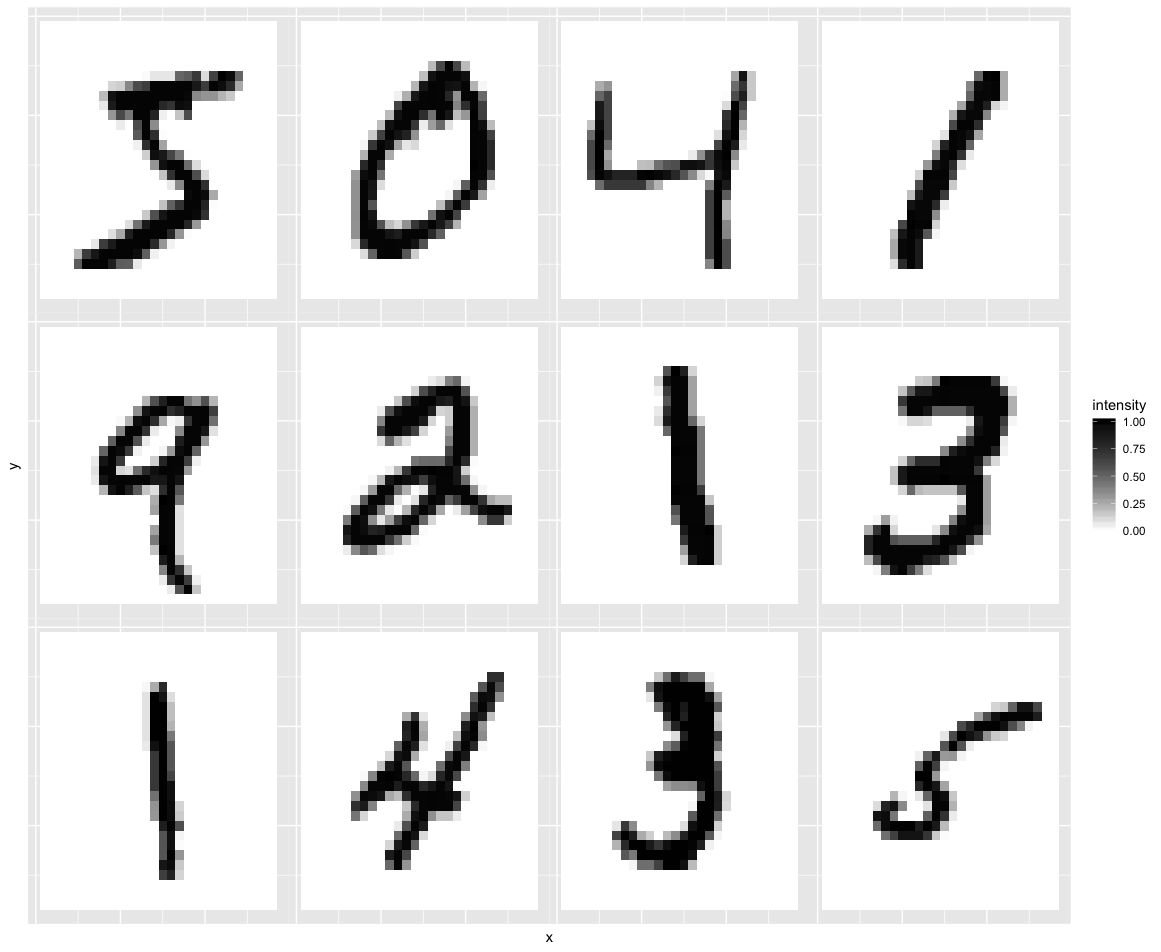
\includegraphics{MNIST2.png}

Each digit has been converted to a grid of \(28\times 28\) pixels, with a grayscale intensity level specified for each pixel. When we store these on a computer, we flatten each grid to a vector of length 784.
So for this dataset, \(n=60,000\) and \(p=784\). As an example of what the data look like, the intensities (times 100) for the first image above are shown in the plot below:

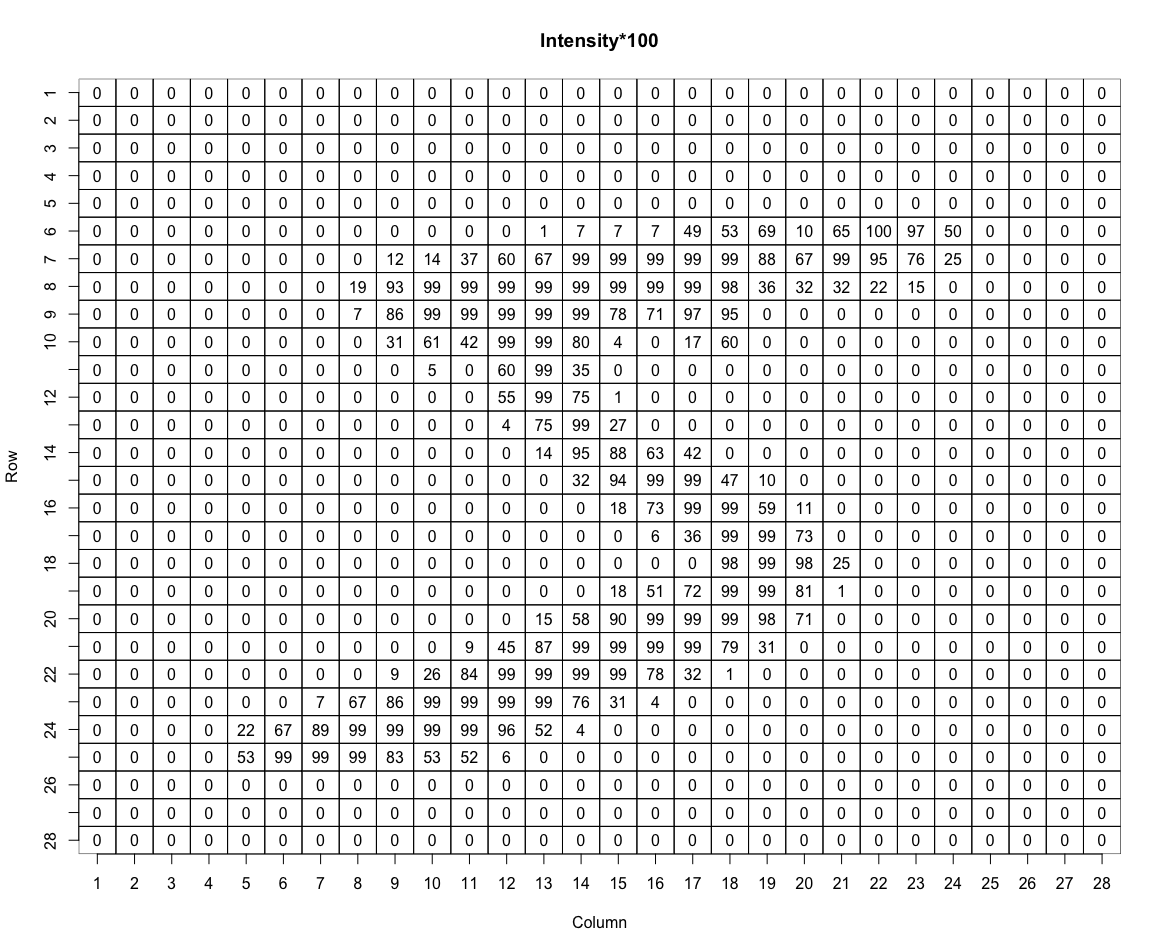
\includegraphics{MNIST3.png}
\end{example}

\subsection{Aims of multivariate data analysis}\label{aims-of-multivariate-data-analysis}

The aim of multivariate statistical analysis is to answer questions such as:

\begin{itemize}
\tightlist
\item
  How can we visualise the data?
\item
  What is the joint distribution of marks?
\item
  Can we simplify the data? For example, we rank football teams using \(3W+D\) and we rank students by their average module mark. Is this fair? Can we reduce the dimension in a better way?
\item
  Can we use the data to discriminate, for example, between male and female students?
\item
  Are the different iris species different shapes?
\item
  Can we build a model to predict the intended digit from an image of someones handwriting? Or predict the species of iris from measurements of its sepal and petal?
\end{itemize}

We could just apply standard univariate techniques to each variable in turn, but this ignores possible dependencies between the variables which we must represent to draw valid conclusions.

\textbf{What is the difference between MVA and standard linear regression?}

\begin{itemize}
\tightlist
\item
  In standard linear regression we have a scalar response variable, \(y\) say, and a vector of covariates, \(\mathbf x\), say. The focus of interest is on how knowledge of \(\mathbf x\) influences the distribution of \(y\) (in particular, the mean of \(y\)). In contrast, in MVA the focus is a vector \(\mathbf y\), in which all the components of \(\mathbf y\) are viewed as responses rather than covariates, possibly with additional covariate information \(\mathbf x\). We will discuss this further in Chapter \ref{lm}.
\end{itemize}

\section{Exploratory data analysis (EDA)}\label{exploratory-data-analysis-eda}

\begin{quote}
A picture is worth a thousand words
\end{quote}

\begin{figure}
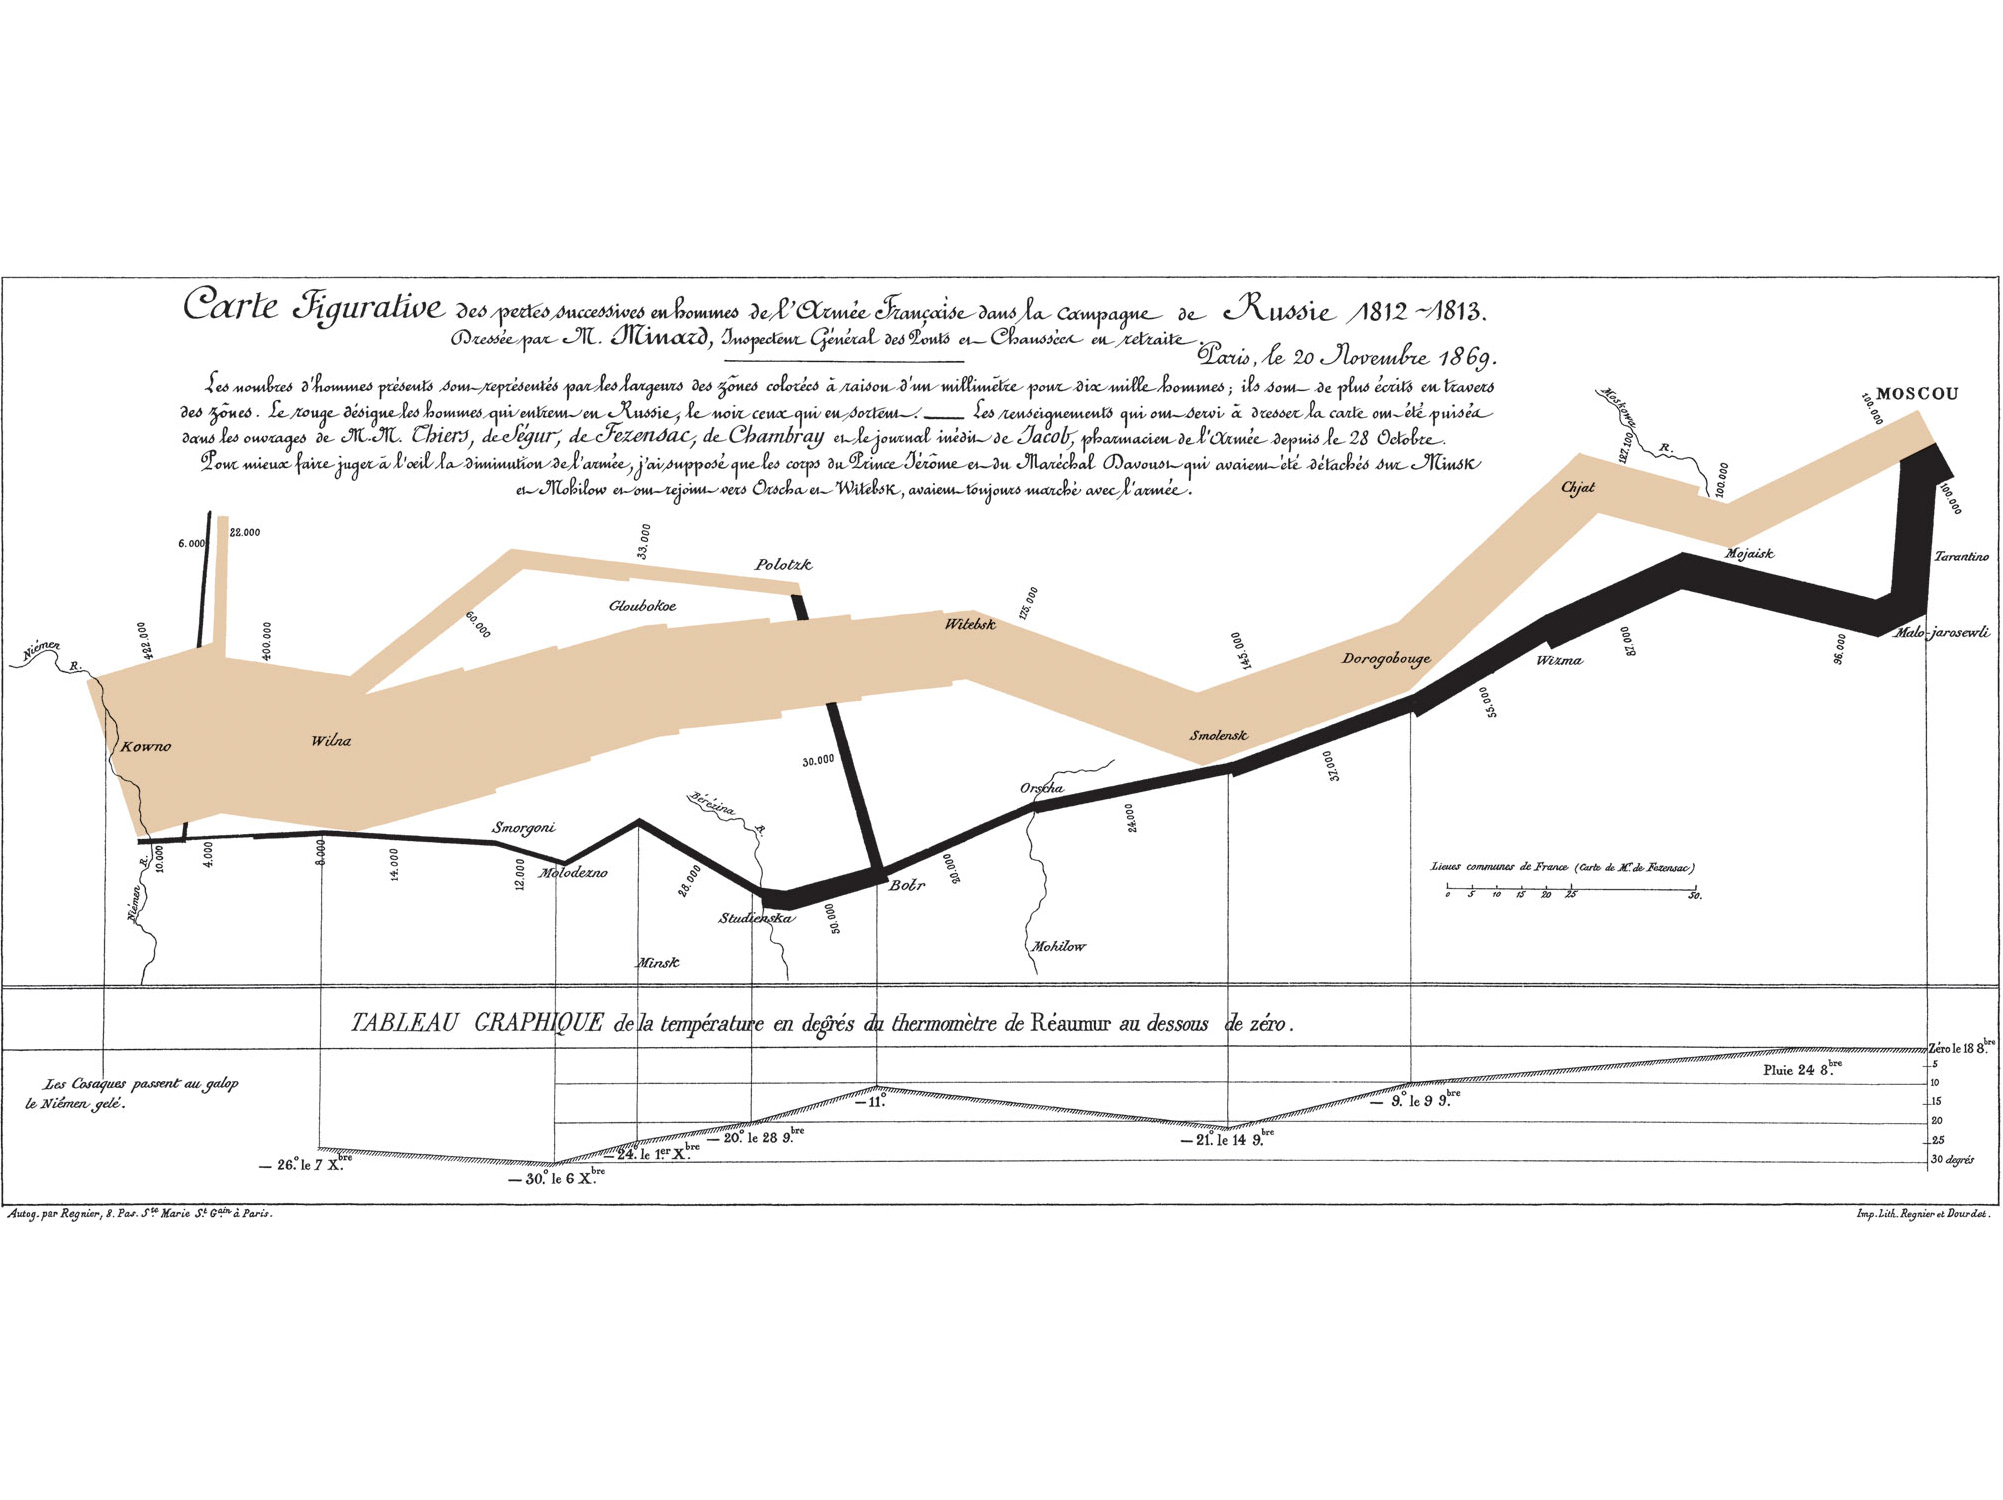
\includegraphics[width=1\linewidth]{figs/Minard} \caption{Charles Joseph Minard's famous map of Napoleons 1812 invasion of Russian. It displays six types of data in two dimensions. See wikipedia page for Charles Joseph Minard.}\label{fig:unnamed-chunk-5}
\end{figure}

Before trying any form of statistical analysis, it is always a good idea to do some form of exploratory data analysis to understand the challenges presented by the data. As a minimum, this usually involves finding out whether each variable is continuous, discrete, or categorical, doing some basic visualization (plots), and perhaps computing a few summary statistics such as the mean and variance.

\subsection{Data visualization}\label{data-visualization}

Visualising datasets before fitting any models can be extremely useful. It allows us to see obvious patterns and relationships, and may suggest a sensible form of analysis.
With multivariate data, finding the right kind of plot is not always simple, and many different approaches have been proposed.

When \(p=1\) or \(p=2\) we can simply draw histograms and scatter plots (respectively) to view the distribution. For \(p \geq 3\) the task is harder. One solution is a matrix of pair-wise scatter plots using the \texttt{pairs} command in R. The graph below shows the relationship between goals scored (F), goals against (A) and points (PT) for 20 teams during a recent Premiership season.

\begin{figure}
\centering
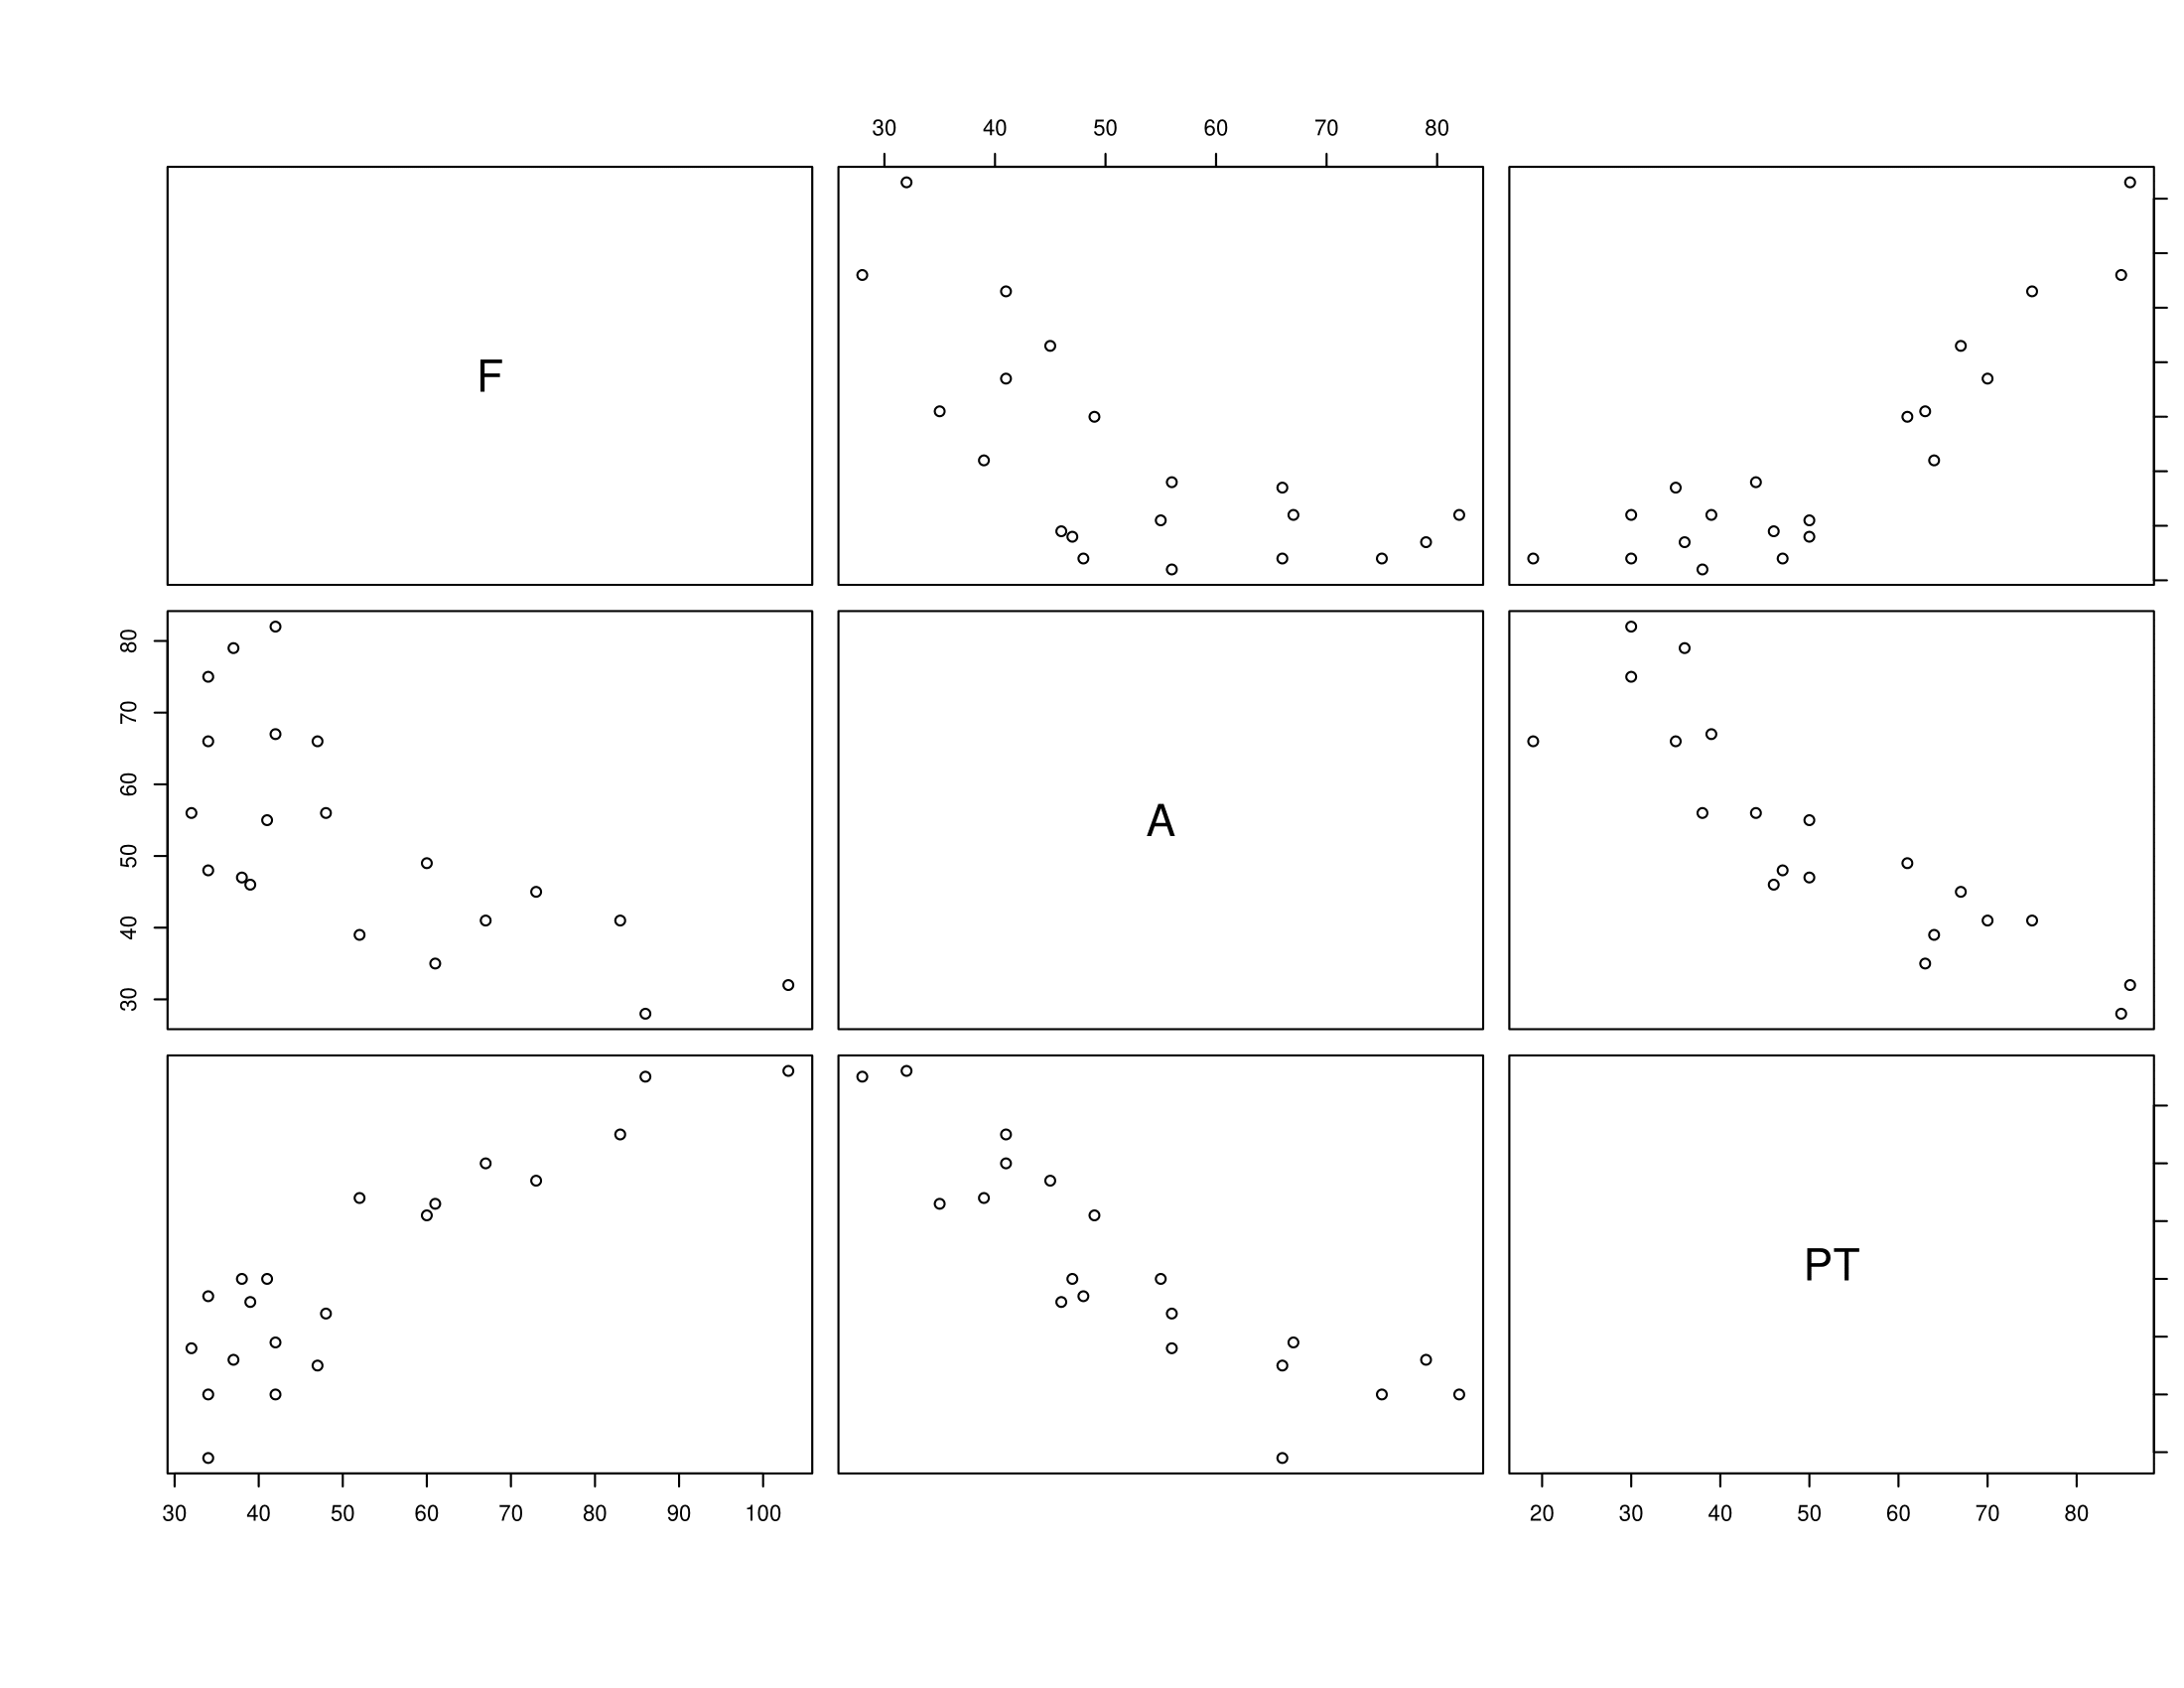
\includegraphics{figs/pairs.png}
\caption{\label{fig:unnamed-chunk-6}Scatter plots of goals for (F), goals against (A) and points (PT) for a recent Premier League Season}
\end{figure}

We can instantly see that points and goals scored are positively correlated, and that points and goals conceded (A) are negatively correlated (this is not a surprise of course).

R has a good basic plotting functionality. However, we will sometimes use packages that provide additional functionality. The first time you use a package you may need to install it. We can use \texttt{ggplot2} and \texttt{GGally} (which adds functionality to \texttt{ggplot2}) to add colour and detail to pairs plots. For example

\begin{Shaded}
\begin{Highlighting}[]
\FunctionTok{data}\NormalTok{(iris)}
\FunctionTok{library}\NormalTok{(ggplot2)}
\FunctionTok{library}\NormalTok{(GGally)}
\CommentTok{\# pairs(iris) \# {-} try the pairs command for comparison}
\FunctionTok{ggpairs}\NormalTok{(iris, }\AttributeTok{columns=}\DecValTok{1}\SpecialCharTok{:}\DecValTok{4}\NormalTok{,  }\AttributeTok{mapping=}\NormalTok{ggplot2}\SpecialCharTok{::}\FunctionTok{aes}\NormalTok{(}\AttributeTok{colour =}\NormalTok{ Species),}
        \AttributeTok{upper =} \FunctionTok{list}\NormalTok{(}\AttributeTok{continuous =} \FunctionTok{wrap}\NormalTok{(}\StringTok{"cor"}\NormalTok{, }\AttributeTok{size =} \DecValTok{3}\NormalTok{)))  }
\end{Highlighting}
\end{Shaded}

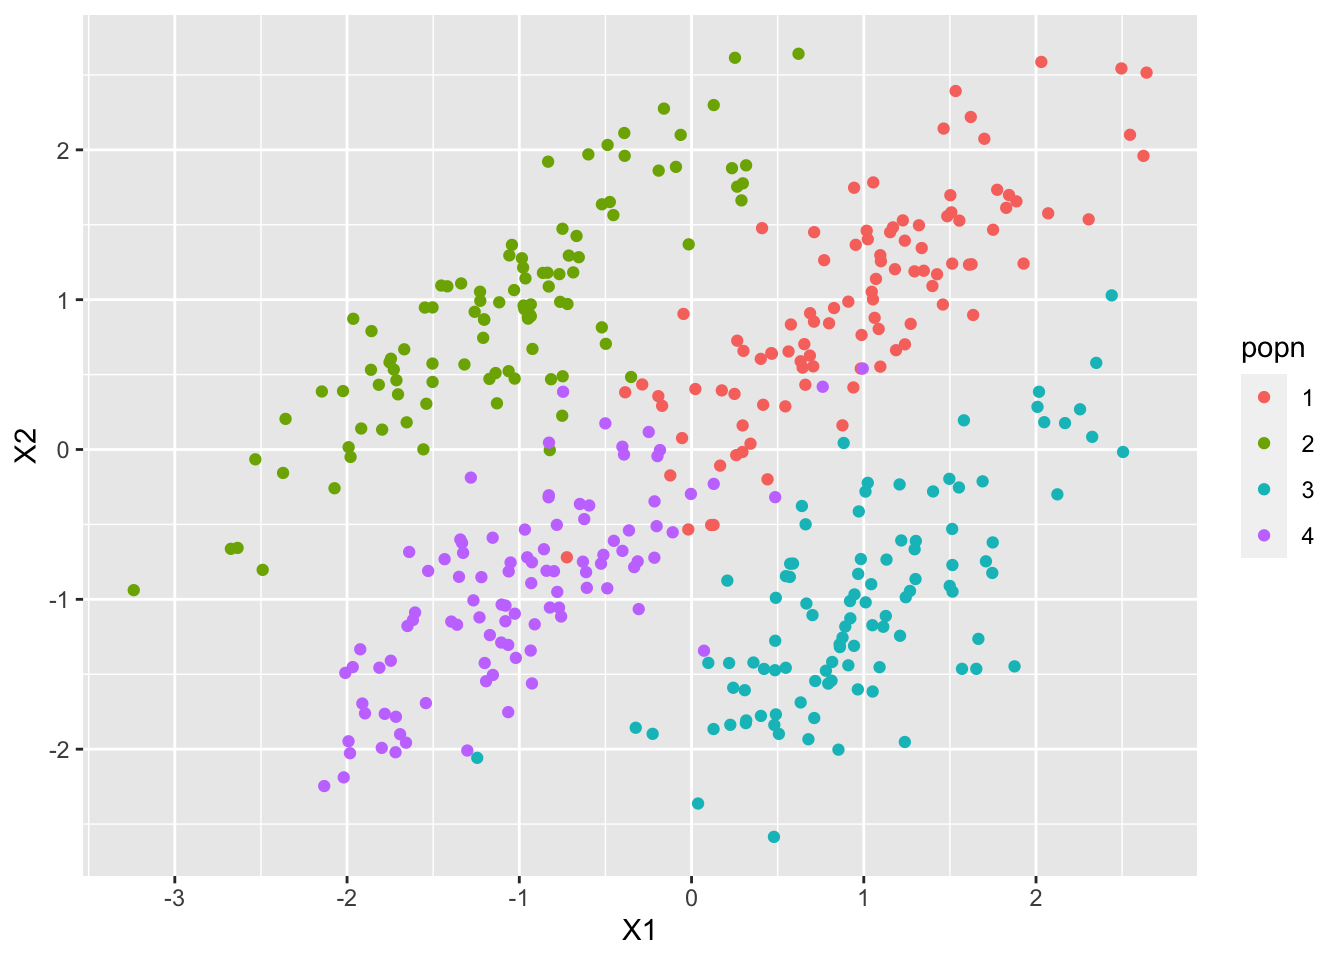
\includegraphics[width=1\linewidth]{01-statistical-prelim_files/figure-latex/unnamed-chunk-7-1}

This plot allows us to instantly see that there are clear differences between the three species of iris, at least when we look at the pairs plots. The benefit of adding colour in this case is that we can see the differences between the different species. Note how the sepal length and width are (weakly) negatively correlated across the entire dataset, but are positively correlated when we look at a single species at a time. We would have missed this information if we only used the \texttt{pairs} command (try it!).

Note that it is possible to miss key relationships when looking at \emph{marginals} plots such as these, as they only show two variables at a time. More complex relationships between three or more variables will not be visible. It is difficult visualize data in three or more dimensions. Many different types of plot have been proposed (e.g.~Google Chernoff faces). One approach is to use a \emph{parallel line} plot

\begin{Shaded}
\begin{Highlighting}[]
\FunctionTok{ggparcoord}\NormalTok{(iris, }\DecValTok{1}\SpecialCharTok{:}\DecValTok{4}\NormalTok{, }\AttributeTok{groupColumn=}\DecValTok{5}\NormalTok{)}
\end{Highlighting}
\end{Shaded}

\includegraphics{01-statistical-prelim_files/figure-latex/unnamed-chunk-8-1.pdf}

Each case is represented by a single line, and here we have the information shown for the four continuous variables. The fifth variable \texttt{Species} is a discrete factor, and is shown by colouring the lines.

If you not familiar with \texttt{ggplot2}, a nice introduction can be found \href{https://ggplot2.tidyverse.org/}{here}. Details about `GGally can be found \href{https://ggobi.github.io/ggally/}{here}. A good way to see the variety of plots that are possible, and to find code to create them, is to browse plot galleries such as those available
\href{https://www.r-graph-gallery.com/ggplot2-package.html}{here}
and \href{https://www.data-to-viz.com}{here}.

\subsection{Summary statistics}\label{summary-statistics}

It is often useful to report a small number of numerical summaries of the data.
In univariate statistics we define the sample mean and sample variance of samples \(x_1, \ldots, x_n\) to be
\[ \bar{x} = \frac{1}{n} \sum_{i=1}^n x_i \quad \text{and} \quad s_{xx} = \frac{1}{n} \sum_{i=1}^n (x_i - \bar{x})^2 \]
and for two samples, \(x_1, \ldots, x_n\) and \(y_1, \ldots, y_n\), we define the sample covariance to be
\[s_{xy}=\frac{1}{n}\sum_{i=1}^n (x_i-\bar{x})(y_i-\bar{y}).\]

Analogous multivariate quantities can be defined as follows:

\begin{definition}
\protect\hypertarget{def:samplemean}{}\label{def:samplemean}For a sample of \(n\) points, each containing \(p\) variables, \(\mathbf x_1, \mathbf x_2, \ldots, \mathbf x_n \in \mathbb{R}^p\), the \textbf{sample mean} and \textbf{sample covariance matrix} are
\begin{align}
 \bar{\mathbf x} &= \frac{1}{n} \sum_{i=1}^n \mathbf x_i \label{eq:samplemean}\\
 \mathbf S&= \frac{1}{n} \sum_{i=1}^n (\mathbf x_i - \bar{\mathbf x}) (\mathbf x_i - \bar{\mathbf x})^\top 
\label{eq:samplecov}
\end{align}
where \(\mathbf x_i\in \mathbb{R}^p\) denotes the \(p\) variables observed on the \(i\)th subject.
\end{definition}

Note that

\begin{itemize}
\tightlist
\item
  \(\bar{\mathbf x} \in \mathbb{R}^p\). The \(j\)th entry in \(\bar{\mathbf x}\) is simply the (univariate) sample mean of the \(j\)th variable.
\item
  \(\mathbf S\in \mathbb{R}^{p\times p}\). Note that the \(ij^{th}\) entry of \(\mathbf S\) is \(s_{ij}\), the sample covariance between variable \(i\) and variable \(j\). The \(i^{th}\) diagonal element is the (univariate) sample variance of the \(i\)th variable.\\
\item
  \(\mathbf S\) is symmetric since \(s_{ij}=s_{ji}\).
\item
  an alternative formula for \(\mathbf S\) is
  \[\mathbf S= \frac{1}{n} \left(\sum_{i=1}^n \mathbf x_i \mathbf x_i^\top \right)- \bar{\mathbf x} \bar{\mathbf x}^\top.\]
\item
  We have divided by \(n\) rather than \(n-1\) here, which gives the maximum likelihood estimator of the variance, rather than the unbiased variance estimator that is often used.
\end{itemize}

\begin{definition}
\protect\hypertarget{def:samplecor}{}\label{def:samplecor}The \textbf{sample correlation matrix}, \(\mathbf R\), is the matrix with \(ij^{th}\) entry \(r_{ij}\) equal to the sample correlation between variables \(i\) and \(j\), that is
\[ r_{ij} = \frac{s_{ij}}{\sqrt{s_{ii}s_{jj}}}. \]
\end{definition}

Note that

\begin{itemize}
\tightlist
\item
  If \(\mathbf D= \text{diag}(\sqrt{s_{11}}, \dots, \sqrt{s_{pp}})\), then\\
  \[ \mathbf R= \mathbf D^{-1} \mathbf S\mathbf D^{-1} \]
\item
  \(\mathbf R\) is symmetric
\item
  the diagonal entries of \(\mathbf R\) are exactly 1 (each variable is perfectly correlated with itself)
\item
  \(|r_{ij}| \leq 1\) for all \(i, j\)
\end{itemize}

Note that if we change the unit of measurement for the \(\mathbf x_i\)'s then \(\mathbf S\) will change but \(\mathbf R\) will not.

\begin{definition}
\protect\hypertarget{def:totalvar}{}\label{def:totalvar}The \textbf{total variation} in a data set is usually measured by \(\text{tr}(\mathbf S)\) where \(\text{tr}()\) is the trace function that sums the diagonal elements of the matrix. That is,
\[\text{tr}(\mathbf S) = s_{11} + s_{22} + \ldots + s_{pp}.\]
In other words, it is the sum of the univariate variances of each of the \(p\) variables.
\end{definition}

\section{Random vectors and matrices}\label{randvec}

\begin{definition}
\protect\hypertarget{def:popmean}{}\label{def:popmean}The \textbf{population mean vector} of the random vector \(\mathbf x\) is
\[{\boldsymbol{\mu}}= {\mathbb{E}}(\mathbf x).\]

The \textbf{population covariance matrix} of \(\mathbf x\) is
\[ \boldsymbol{\Sigma}= {\mathbb{V}\operatorname{ar}}(\mathbf x) = {\mathbb{E}}\left((\mathbf x-{\mathbb{E}}(\mathbf x))(\mathbf x-{\mathbb{E}}(\mathbf x))^\top \right).\]

The \textbf{covariance} between \(\mathbf x\) (\(p \times 1\)) and \(\mathbf y\) (\(q \times 1\)) is
\[ {\mathbb{C}\operatorname{ov}}(\mathbf x,\mathbf y) = {\mathbb{E}}\left((\mathbf x- {\mathbb{E}}(\mathbf x))(\mathbf y- {\mathbb{E}}(\mathbf y))^\top \right). \]
\end{definition}

Let \(\mathbf A\) denote a \(q \times p\) constant matrix, and let \(\mathbf b\) a constant vector of size \(q \times 1\).
Expectation is a linear operator in the sense that

\[{\mathbb{E}}(\mathbf A\mathbf x+ \mathbf b) = \mathbf A{\mathbb{E}}(\mathbf x) + \mathbf b=\mathbf A{\boldsymbol{\mu}}+\mathbf b.\]

The following properties follow:

\begin{itemize}
\tightlist
\item
  \({\mathbb{V}\operatorname{ar}}(\mathbf x) = {\mathbb{E}}(\mathbf x\mathbf x^\top) - {\boldsymbol{\mu}}{\boldsymbol{\mu}}^\top\).
\item
  \({\mathbb{V}\operatorname{ar}}(\mathbf A\mathbf x+ \mathbf b) = \mathbf A\boldsymbol{\Sigma}\mathbf A^\top\)
\item
  \({\mathbb{C}\operatorname{ov}}(\mathbf x,\mathbf y) = {\mathbb{E}}(\mathbf x\mathbf y^\top) - {\mathbb{E}}(\mathbf x) {\mathbb{E}}(\mathbf y)^\top\).
\item
  \({\mathbb{C}\operatorname{ov}}(\mathbf x,\mathbf x) = \boldsymbol{\Sigma}\).
\item
  \({\mathbb{C}\operatorname{ov}}(\mathbf x,\mathbf y) = {\mathbb{C}\operatorname{ov}}(\mathbf y,\mathbf x)^\top\).
\item
  \({\mathbb{C}\operatorname{ov}}(\mathbf A\mathbf x,\mathbf B\mathbf y) = \mathbf A{\mathbb{C}\operatorname{ov}}(\mathbf x,\mathbf y)\mathbf B^\top\)
\item
  If \(p=q\) then
  \[
  {\mathbb{V}\operatorname{ar}}(\mathbf x+ \mathbf y) = {\mathbb{V}\operatorname{ar}}(\mathbf x) + {\mathbb{V}\operatorname{ar}}(\mathbf y) + {\mathbb{C}\operatorname{ov}}(\mathbf x,\mathbf y) + {\mathbb{C}\operatorname{ov}}(\mathbf y,\mathbf x).
  \]
\end{itemize}

Finally, note that if \(\mathbf x\) and \(\mathbf y\) are independent (in which case I will write \(\mathbf x\perp \!\!\! \perp\mathbf y\)) then \({\mathbb{C}\operatorname{ov}}(\mathbf x,\mathbf y) = {\mathbf 0}_{p,q}\), i.e., a \(p\times q\) matrix of zeros.

\subsection{Estimators}\label{estimators}

The population mean vector \({\boldsymbol{\mu}}\) and population covariance matrix \(\boldsymbol{\Sigma}\) will usually be unknown. We can use data to \textbf{estimate} these quantities.

\begin{itemize}
\tightlist
\item
  The sample mean \(\bar{\mathbf x}\) is often used as an estimator of \({\boldsymbol{\mu}}\).
\item
  The sample covariance matrix \(\mathbf S\) is often used as an estimator of \(\boldsymbol{\Sigma}\).
\end{itemize}

Equation \eqref{eq:samplemean} gives an unbiased estimator of the sample mean. The sample covariance matrix \eqref{eq:samplecov} is a biased estimator of the population covariance matrix. An unbiased estimate is obtained by dividing by \(n-1\) rather than \(n\) in Equation \eqref{eq:samplecov}.

\section{Computer tasks}\label{computer-tasks}

If you haven't done so already, please download and install R and Rstudio. R is the programming language, and Rstudio is an integrated development environment that makes using R much more pleasurable. My advice is to always use Rstudio and never run code in R itself.

\begin{enumerate}
\def\labelenumi{\arabic{enumi}.}
\setcounter{enumi}{-1}
\item
  \textbf{For complete beginners:} For those who are completely new to R (or those who want a refresher), I recommend working through an online tutorial. \href{https://www.statmethods.net/r-tutorial/index.html}{This} tutorial looks good, but contains more than you'll need.
\item
  \textbf{Warm-up:} The most important aspects of R to focus on for this module are

  \begin{itemize}
  \tightlist
  \item
    Basic plotting
  \item
    Manipulation of matrices and data frames.
  \end{itemize}

  Let's look at the \texttt{iris} dataset.

  \begin{itemize}
  \tightlist
  \item
    Can you plot the sepal length against the sepal width?
  \end{itemize}

  We'll now do some exercises on data manipulation. Note that there are several ways to do basic data manipulation in R. You can use base R commands or if you prefer, you can use the \href{https://dplyr.tidyverse.org/}{dplyr} commands which are part of the \texttt{tidyverse} packages.
  For example, to select columns, in base you can do:
\end{enumerate}

\begin{Shaded}
\begin{Highlighting}[]
\NormalTok{iris[,}\DecValTok{2}\NormalTok{] }\CommentTok{\# selects column 2}
\NormalTok{iris}\SpecialCharTok{$}\NormalTok{Sepal.Width }\CommentTok{\# selects the same column by name}
\end{Highlighting}
\end{Shaded}

or using dplyr you can do

\begin{Shaded}
\begin{Highlighting}[]
\FunctionTok{library}\NormalTok{(dplyr)}
\FunctionTok{select}\NormalTok{(iris, }\StringTok{"Sepal.Width"}\NormalTok{)}
\end{Highlighting}
\end{Shaded}

\begin{itemize}
\item
  Can you select the column of the \texttt{iris} data that contains just the sepal length and add it to the sepal width?

  To select only certain rows of the data (i.e.~to filter it), we can again use either base R or dplyr.
\end{itemize}

\begin{Shaded}
\begin{Highlighting}[]
\NormalTok{iris[iris[,}\DecValTok{3}\NormalTok{]}\SpecialCharTok{\textless{}}\DecValTok{5}\NormalTok{,] }
\CommentTok{\# select all rows that have a petal length less than 5.}
\FunctionTok{filter}\NormalTok{(iris, Petal.Length}\SpecialCharTok{\textless{}}\DecValTok{5}\NormalTok{) }\CommentTok{\# do the same thing using dplyr}
\end{Highlighting}
\end{Shaded}

\begin{itemize}
\item
  Can you now select all the rows of the \texttt{iris} data frame that are for species \emph{setosa}? What is the mean petal length for these flowers?
\item
  Can you select all the flowers that have a sepal length greater than 5? What is the proportion of each species of iris in this set?
\end{itemize}

A nice aspect of dplyr is that you can chain commmands together. So for example, to select the versicolour flowers with petal width less than 1.5, we can do

\begin{Shaded}
\begin{Highlighting}[]
\NormalTok{iris }\SpecialCharTok{|\textgreater{}} \FunctionTok{filter}\NormalTok{(Species}\SpecialCharTok{==}\StringTok{\textquotesingle{}versicolor\textquotesingle{}}\NormalTok{) }\SpecialCharTok{|\textgreater{}} \FunctionTok{filter}\NormalTok{(Petal.Width}\SpecialCharTok{\textless{}}\FloatTok{1.5}\NormalTok{)}
\end{Highlighting}
\end{Shaded}

\begin{itemize}
\tightlist
\item
  Can you select all the flowers that have a sepal length greater than 6, and a petal length less than 5? What is the proportion of each species in this set?
\end{itemize}

Note that \texttt{iris} is a data frame

\begin{Shaded}
\begin{Highlighting}[]
\FunctionTok{is.data.frame}\NormalTok{(iris)}
\end{Highlighting}
\end{Shaded}

\begin{verbatim}
## [1] TRUE
\end{verbatim}

which is a type of structure used in R. This is convenient for some tasks, but not for others. Let's first extract the four numerical columns and store them as a matrix \(X\).

\begin{Shaded}
\begin{Highlighting}[]
\FunctionTok{is.matrix}\NormalTok{(iris)}
\end{Highlighting}
\end{Shaded}

\begin{verbatim}
## [1] FALSE
\end{verbatim}

\begin{Shaded}
\begin{Highlighting}[]
\NormalTok{X }\OtherTok{\textless{}{-}} \FunctionTok{as.matrix}\NormalTok{(iris[,}\DecValTok{1}\SpecialCharTok{:}\DecValTok{4}\NormalTok{])}
\FunctionTok{is.matrix}\NormalTok{(X)}
\end{Highlighting}
\end{Shaded}

\begin{verbatim}
## [1] TRUE
\end{verbatim}

\begin{itemize}
\tightlist
\item
  Select the 4 numerical columns and multiply the first column by 1, the second by 2, the third by 3, and the 4th by 4. One way to do this is by multiplying \(X\) by the diagonal matrix
\end{itemize}

\begin{Shaded}
\begin{Highlighting}[]
\FunctionTok{diag}\NormalTok{(}\DecValTok{1}\SpecialCharTok{:}\DecValTok{4}\NormalTok{)}
\end{Highlighting}
\end{Shaded}

\begin{verbatim}
##      [,1] [,2] [,3] [,4]
## [1,]    1    0    0    0
## [2,]    0    2    0    0
## [3,]    0    0    3    0
## [4,]    0    0    0    4
\end{verbatim}

\begin{enumerate}
\def\labelenumi{\arabic{enumi}.}
\setcounter{enumi}{1}
\tightlist
\item
  The table below shows the module marks for 5 students on the modules G11PRB (\(P\)) and G11STA (\(S\)).
\end{enumerate}

\begin{table}
\centering
\begin{tabular}{lrr}
\toprule
Student & P & S\\
\midrule
A & 41 & 63\\
B & 72 & 82\\
C & 46 & 38\\
D & 77 & 57\\
E & 59 & 85\\
\bottomrule
\end{tabular}
\end{table}

\begin{itemize}
\tightlist
\item
  As an exercise, calculate the sample mean, sample covariance, and sample correlation by hand.
\end{itemize}

\begin{itemize}
\tightlist
\item
  Now calculate these in R using \texttt{colMeans}, \texttt{cov}, and \texttt{cor}. These commands assume each column is a different variable, and each row a different observation.
  \textbf{Note that} by default R uses \(n-1\) in the denominator for the variance and covariance commands, whereas we used \(n\) in our definition.
\end{itemize}

You can load the data into R using the following commands:

\begin{Shaded}
\begin{Highlighting}[]
\NormalTok{Ex1 }\OtherTok{\textless{}{-}} \FunctionTok{data.frame}\NormalTok{(}
  \AttributeTok{Student=}\NormalTok{LETTERS[}\DecValTok{1}\SpecialCharTok{:}\DecValTok{5}\NormalTok{],}
  \AttributeTok{P =} \FunctionTok{c}\NormalTok{(}\DecValTok{41}\NormalTok{,}\DecValTok{72}\NormalTok{,}\DecValTok{46}\NormalTok{,}\DecValTok{77}\NormalTok{,}\DecValTok{59}\NormalTok{),}
  \AttributeTok{S =} \FunctionTok{c}\NormalTok{(}\DecValTok{63}\NormalTok{,}\DecValTok{82}\NormalTok{,}\DecValTok{38}\NormalTok{,}\DecValTok{57}\NormalTok{,}\DecValTok{85}\NormalTok{)}
\NormalTok{  )}
\end{Highlighting}
\end{Shaded}

\begin{itemize}
\tightlist
\item
  Can you compute the covariance matrix using the definition in Equation \eqref{eq:samplecov}?
\end{itemize}

\begin{enumerate}
\def\labelenumi{\arabic{enumi}.}
\setcounter{enumi}{2}
\tightlist
\item
  The \texttt{mtcars} dataset is another built-in dataset in R. You can read about it by typing \texttt{?mtcars} in R. Note that some of the variables are factors. You can ensure R treats them as factors by using the following command to create a dataset where they are listed as factors:
\end{enumerate}

\begin{Shaded}
\begin{Highlighting}[]
\NormalTok{mtcars2 }\OtherTok{\textless{}{-}} \FunctionTok{within}\NormalTok{(mtcars, \{}
\NormalTok{   vs }\OtherTok{\textless{}{-}} \FunctionTok{factor}\NormalTok{(vs, }\AttributeTok{labels =} \FunctionTok{c}\NormalTok{(}\StringTok{"V"}\NormalTok{, }\StringTok{"S"}\NormalTok{))}
\NormalTok{   am }\OtherTok{\textless{}{-}} \FunctionTok{factor}\NormalTok{(am, }\AttributeTok{labels =} \FunctionTok{c}\NormalTok{(}\StringTok{"automatic"}\NormalTok{, }\StringTok{"manual"}\NormalTok{))}
\NormalTok{   cyl  }\OtherTok{\textless{}{-}} \FunctionTok{ordered}\NormalTok{(cyl)}
\NormalTok{   gear }\OtherTok{\textless{}{-}} \FunctionTok{ordered}\NormalTok{(gear)}
\NormalTok{   carb }\OtherTok{\textless{}{-}} \FunctionTok{ordered}\NormalTok{(carb)}
\NormalTok{\})}
\end{Highlighting}
\end{Shaded}

Work with the \texttt{mtcars2} dataframe when you use \texttt{ggplot2}.

\begin{itemize}
\tightlist
\item
  Create some plots to explore the structure of this dataset using ggplot2.
\item
  Try using the \texttt{pairs} command from base R and the \texttt{ggpairs} command from GGally.
\item
  Try colouring the scatter plots accoring to whether the car is automatic or not.
\item
  Create another plot using colour to represent the number of gears.
\item
  Find another type of plot from one of the plot galleries and try to create a similar plot with these data.
\end{itemize}

\begin{enumerate}
\def\labelenumi{\arabic{enumi}.}
\setcounter{enumi}{3}
\tightlist
\item
  We can 100 generate samples from the multivariate normal distribution with mean vector
  \[{\boldsymbol{\mu}}= \left(\begin{array}{c}1\\0\end{array}\right)\]
  and covariance matrix
  \[\boldsymbol{\Sigma}= \left(\begin{array}{cc}2&1\\1&2\end{array}\right)\]
  as follows (you may need to install the R package \texttt{mvtnorm} first):
\end{enumerate}

\begin{Shaded}
\begin{Highlighting}[]
\FunctionTok{library}\NormalTok{(mvtnorm)}
\NormalTok{mu }\OtherTok{=} \FunctionTok{c}\NormalTok{(}\DecValTok{1}\NormalTok{,}\DecValTok{0}\NormalTok{)}
\NormalTok{Sigma}\OtherTok{=}\FunctionTok{matrix}\NormalTok{(}\FunctionTok{c}\NormalTok{(}\DecValTok{2}\NormalTok{,}\DecValTok{1}\NormalTok{,}\DecValTok{1}\NormalTok{,}\DecValTok{2}\NormalTok{), }\AttributeTok{nr=}\DecValTok{2}\NormalTok{)}
\NormalTok{X }\OtherTok{\textless{}{-}} \FunctionTok{rmvnorm}\NormalTok{(}\AttributeTok{n=}\DecValTok{100}\NormalTok{, }\AttributeTok{mean=}\NormalTok{mu, }\AttributeTok{sigma=}\NormalTok{Sigma)}
\end{Highlighting}
\end{Shaded}

\begin{itemize}
\tightlist
\item
  Compute the sample mean and covariance matrix of these samples.
\item
  Generate a new sample dataset, \(X\), and recompute the sample mean and covariance matrix. What do you notice?
\item
  Try changing \(n\), the number of samples (making it much larger say), and now recomputing the mean and covariance. What do you notice?
\end{itemize}

\begin{enumerate}
\def\labelenumi{\arabic{enumi}.}
\setcounter{enumi}{4}
\tightlist
\item
  \textbf{Optional} Download the MNIST data from Moodle and load it into R.
\end{enumerate}

\begin{Shaded}
\begin{Highlighting}[]
\FunctionTok{load}\NormalTok{(}\StringTok{\textquotesingle{}mnist.rda\textquotesingle{}}\NormalTok{)}
\end{Highlighting}
\end{Shaded}

This loads a list \texttt{mnist} that splits the data into two parts

\begin{Shaded}
\begin{Highlighting}[]
\NormalTok{mnist}\SpecialCharTok{$}\NormalTok{train }\DocumentationTok{\#\# a training set of 60000 images}
\NormalTok{mnist}\SpecialCharTok{$}\NormalTok{test }\DocumentationTok{\#\# a test set of 10000 images}
\end{Highlighting}
\end{Shaded}

Let's just look at the training set. This is also a list containing the image intensities and the image labels

\begin{Shaded}
\begin{Highlighting}[]
\NormalTok{mnist}\SpecialCharTok{$}\NormalTok{train}\SpecialCharTok{$}\NormalTok{x }\CommentTok{\# image intensities}
\NormalTok{mnist}\SpecialCharTok{$}\NormalTok{train}\SpecialCharTok{$}\NormalTok{y }\CommentTok{\# image labels}
\end{Highlighting}
\end{Shaded}

If we select just the first image we can see it is a vector of length 784 containing numbers between 0 and 1.

\begin{Shaded}
\begin{Highlighting}[]
\NormalTok{mnist}\SpecialCharTok{$}\NormalTok{train}\SpecialCharTok{$}\NormalTok{x[}\DecValTok{1}\NormalTok{,]}
\end{Highlighting}
\end{Shaded}

I've created a function to help you plot these images.

\begin{Shaded}
\begin{Highlighting}[]
\FunctionTok{library}\NormalTok{(reshape2)}
\FunctionTok{library}\NormalTok{(ggplot2)}


\NormalTok{plot.mnist }\OtherTok{\textless{}{-}} \ControlFlowTok{function}\NormalTok{(im)\{}
  \CommentTok{\#im[im\textless{}0]\textless{}{-}0 \# set any negative intensities to zero}
  \CommentTok{\#im[im\textgreater{}1]\textless{}{-}1 \# set an intensities bigger than 1 to 1.}
  
  
  \ControlFlowTok{if}\NormalTok{(}\FunctionTok{is.vector}\NormalTok{(im))\{ }\CommentTok{\# a single image}
    
\NormalTok{    A}\OtherTok{\textless{}{-}}\FunctionTok{matrix}\NormalTok{(im, }\AttributeTok{nr=}\DecValTok{28}\NormalTok{, }\AttributeTok{byrow=}\NormalTok{F)}
\NormalTok{    C}\OtherTok{\textless{}{-}} \FunctionTok{melt}\NormalTok{(A, }\AttributeTok{varnames =} \FunctionTok{c}\NormalTok{(}\StringTok{"x"}\NormalTok{, }\StringTok{"y"}\NormalTok{), }
             \AttributeTok{value.name =} \StringTok{"intensity"}\NormalTok{)}
\NormalTok{    p}\OtherTok{\textless{}{-}}\FunctionTok{ggplot}\NormalTok{(C, }\FunctionTok{aes}\NormalTok{(}\AttributeTok{x =}\NormalTok{ x, }\AttributeTok{y =}\NormalTok{ y, }\AttributeTok{fill =}\NormalTok{ intensity))}\SpecialCharTok{+}
      \FunctionTok{geom\_tile}\NormalTok{(}\FunctionTok{aes}\NormalTok{(}\AttributeTok{fill=}\NormalTok{intensity))}\SpecialCharTok{+}
      \FunctionTok{scale\_fill\_gradient}\NormalTok{(}\AttributeTok{low=}\StringTok{\textquotesingle{}white\textquotesingle{}}\NormalTok{, }\AttributeTok{high=}\StringTok{\textquotesingle{}black\textquotesingle{}}\NormalTok{)}\SpecialCharTok{+}
      \FunctionTok{scale\_y\_reverse}\NormalTok{()}\SpecialCharTok{+}\FunctionTok{theme}\NormalTok{(}
        \AttributeTok{strip.background =} \FunctionTok{element\_blank}\NormalTok{(),}
        \AttributeTok{strip.text.x =} \FunctionTok{element\_blank}\NormalTok{(),}
        \AttributeTok{panel.spacing =} \FunctionTok{unit}\NormalTok{(}\DecValTok{0}\NormalTok{, }\StringTok{"lines"}\NormalTok{),}
        \AttributeTok{axis.text =} \FunctionTok{element\_blank}\NormalTok{(),}
        \AttributeTok{axis.ticks =} \FunctionTok{element\_blank}\NormalTok{()}
\NormalTok{      ) }
\NormalTok{  \}}
  \ControlFlowTok{else}\NormalTok{\{}
    \ControlFlowTok{if}\NormalTok{ (}\FunctionTok{dim}\NormalTok{(im)[}\DecValTok{2}\NormalTok{]}\SpecialCharTok{!=}\DecValTok{784}\NormalTok{)\{}
\NormalTok{      im }\OtherTok{=} \FunctionTok{t}\NormalTok{(im)}
\NormalTok{    \} }
\NormalTok{    n }\OtherTok{\textless{}{-}} \FunctionTok{dim}\NormalTok{(im)[}\DecValTok{1}\NormalTok{]}
\NormalTok{    As }\OtherTok{\textless{}{-}} \FunctionTok{array}\NormalTok{(im, }\AttributeTok{dim =} \FunctionTok{c}\NormalTok{(n, }\DecValTok{28}\NormalTok{, }\DecValTok{28}\NormalTok{))}
    
\NormalTok{    Cs}\OtherTok{\textless{}{-}} \FunctionTok{melt}\NormalTok{(As, }\AttributeTok{varnames =} \FunctionTok{c}\NormalTok{(}\StringTok{"image"}\NormalTok{,}\StringTok{"x"}\NormalTok{, }\StringTok{"y"}\NormalTok{), }
              \AttributeTok{value.name =} \StringTok{"intensity"}\NormalTok{)}
\NormalTok{    p}\OtherTok{\textless{}{-}}\FunctionTok{ggplot}\NormalTok{(Cs, }\FunctionTok{aes}\NormalTok{(}\AttributeTok{x =}\NormalTok{ x, }\AttributeTok{y =}\NormalTok{ y, }\AttributeTok{fill =}\NormalTok{ intensity))}\SpecialCharTok{+}
      \FunctionTok{geom\_tile}\NormalTok{(}\FunctionTok{aes}\NormalTok{(}\AttributeTok{fill=}\NormalTok{intensity))}\SpecialCharTok{+}
      \FunctionTok{scale\_fill\_gradient}\NormalTok{(}\AttributeTok{low=}\StringTok{\textquotesingle{}white\textquotesingle{}}\NormalTok{, }\AttributeTok{high=}\StringTok{\textquotesingle{}black\textquotesingle{}}\NormalTok{)}\SpecialCharTok{+}
      \FunctionTok{facet\_wrap}\NormalTok{(}\SpecialCharTok{\textasciitilde{}}\NormalTok{ image, }\AttributeTok{nrow =} \FunctionTok{floor}\NormalTok{(}\FunctionTok{sqrt}\NormalTok{(n))}\SpecialCharTok{+}\DecValTok{1}\NormalTok{, }
                 \AttributeTok{ncol =} \FunctionTok{floor}\NormalTok{(}\FunctionTok{sqrt}\NormalTok{(n))}\SpecialCharTok{+}\DecValTok{1}\NormalTok{)}\SpecialCharTok{+}
      \FunctionTok{scale\_y\_reverse}\NormalTok{()}\SpecialCharTok{+}\FunctionTok{theme}\NormalTok{(}
        \AttributeTok{strip.background =} \FunctionTok{element\_blank}\NormalTok{(),}
        \AttributeTok{strip.text.x =} \FunctionTok{element\_blank}\NormalTok{(),}
        \AttributeTok{panel.spacing =} \FunctionTok{unit}\NormalTok{(}\DecValTok{0}\NormalTok{, }\StringTok{"lines"}\NormalTok{),}
        \AttributeTok{axis.text =} \FunctionTok{element\_blank}\NormalTok{(),}
        \AttributeTok{axis.ticks =} \FunctionTok{element\_blank}\NormalTok{()}
\NormalTok{      ) }
    
\NormalTok{  \}}
  \FunctionTok{return}\NormalTok{(p)}
\NormalTok{\}}
\end{Highlighting}
\end{Shaded}

\begin{itemize}
\item
  Use this command to plot the first 10 images from the MNIST training set.
\item
  Select all the 5s from the MNIST training set. Plot a selection of these digits.
\end{itemize}

\section{Exercises}\label{exercises}

\begin{enumerate}
\def\labelenumi{\arabic{enumi}.}
\item
  Show that the two formulae for the population covariance matrix \(\boldsymbol{\Sigma}\) are equivalent, i.e.~show that
  \[\boldsymbol{\Sigma}= {\mathbb{E}}[(\mathbf x- {\boldsymbol{\mu}}) (\mathbf x- {\boldsymbol{\mu}})^\top ] = {\mathbb{E}}[ \mathbf x\mathbf x^\top ] - {\boldsymbol{\mu}}{\boldsymbol{\mu}}^\top.\]
\item
  Let \(\mathbf x_1, \ldots, \mathbf x_n\) be a \(p\)-dimensional sample with mean \(\bar{\mathbf x}\) and sample covariance matrix \(\mathbf S\). Consider the transformation \(\mathbf y_i = \mathbf A\mathbf x_i + \mathbf c\) where \(\mathbf A\) is a fixed \(q \times p\) matrix and \(\mathbf c\) is a fixed \(q\)-dimensional vector. Let \(\mathbf T\) be the sample covariance matrix of \(\mathbf y_1, \ldots, \mathbf y_n\). Show
\end{enumerate}

\begin{itemize}
\item
  \(\bar{\mathbf y} = \mathbf A\bar{\mathbf x} + \mathbf c\),
\item
  \(\mathbf T= \mathbf A\mathbf S\mathbf A^\top\).
\item
  Assuming now that \(\mathbf x\) is a random vector with \({\mathbb{E}}(\mathbf x)={\boldsymbol{\mu}}\), \({\mathbb{V}\operatorname{ar}}(\mathbf x)=\boldsymbol{\Sigma}\), \(\mathbf y=\mathbf A\mathbf x+\mathbf c\) with \(\mathbf A\) and \(\mathbf c\) as before. Let \({\mathbb{E}}(\mathbf y)={\pmb \phi}\) and \({\mathbb{V}\operatorname{ar}}(\mathbf y)={\pmb \Omega}\) denote the population mean and variance of \(\mathbf y\). What are the analogous population level versions of the sample-based results above (i.e.~express \({\pmb \phi}\) and \({\pmb \Omega}\) in terms of \(\boldsymbol{\Sigma}\), \(\mathbf A\) and \(\mathbf c\))?
\end{itemize}

\begin{enumerate}
\def\labelenumi{\arabic{enumi}.}
\setcounter{enumi}{2}
\item
  A sample of size \(n=144\) produced the following summary statistics
  \[ \sum_{i=1}^n \mathbf x_i = \begin{pmatrix} 392.2 \\ 1530.8 \end{pmatrix} \qquad \sum_{i=1}^n \mathbf x_i \mathbf x_i^\top = \begin{pmatrix} 1101.88 & 4305.17 \\ 4305.17 & 17120.88 \end{pmatrix}.\]
  Calculate the sample mean, the sample covariance matrix and the sample correlation coefficient.
\item
  Let \(\mathbf x\) and \(\mathbf y\) be independent random \(p\)-dimensional vectors. Assuming that all relevant moments exist, show that for any real scalars \(\alpha\) and \(\beta\),
  \[{\mathbb{V}\operatorname{ar}}(\alpha \mathbf x+ \beta \mathbf y) = \alpha^2 {\mathbb{V}\operatorname{ar}}(\mathbf x) + \beta^2 {\mathbb{V}\operatorname{ar}}(\mathbf y).\]

  What is the corresponding formula when \(\mathbf x\) and \(\mathbf y\) are not independent? Express your answer in terms of \({\mathbb{V}\operatorname{ar}}(\mathbf x)\), \({\mathbb{V}\operatorname{ar}}(\mathbf y)\) and \({\mathbb{C}\operatorname{ov}}(\mathbf x, \mathbf y)\).
\item
  You are given the following data points
  \[\mathbf x_1 = \begin{pmatrix} 1\\ 2\end{pmatrix}, \mathbf x_2 = \begin{pmatrix} 2 \\ 2\end{pmatrix}, \mathbf x_3 = \begin{pmatrix} 3\\ 1\end{pmatrix}, \mathbf x_4 = \begin{pmatrix} 0 \\3\end{pmatrix}\]
  Write down the data matrix \(\mathbf X\), the mean vector, and the covariance matrix.
\end{enumerate}

\chapter{Review of linear algebra}\label{linalg-prelim}

Modern statistics and machine learning rely heavily upon linear algebra, nowhere more so than in multivariate statistics. In the first part of this chapter (sections \ref{linalg-basics} and \ref{linalg-vecspaces}) we review some concepts from linear algebra that will be needed throughout the module, including vector spaces, row and column spaces, the rank of a matrix, etc. Hopefully most of this will be familiar to you.

We then cover some basic details on inner-product or normed spaces in \ref{linalg-innerprod}, which are vector spaces equipped with a concept of distance and angle.
Finally, in Section \ref{centering-matrix} we will describe the centering matrix. Further details and proofs for this section will be tackled in the exercises in Section \ref{exercises-ch2}.

I do not provide proofs for many of the results stated in this chapter, but instead prove a small selection which I think it is useful to see. For a complete treatment of the linear algebra needed for this module, see the excellent book ``Linear algebra and learning from data'' by Gilbert Strang.

I have recorded videos on some (but not all) of the topics in these notes:

\begin{itemize}
\tightlist
\item
  \href{https://mediaspace.nottingham.ac.uk/media/Vector+Spaces/1_48xqrp04}{Vector spaces}
\item
  \href{https://mediaspace.nottingham.ac.uk/media/Matrices/1_nqo2u7zs}{Matrices}
\item
  \href{https://mediaspace.nottingham.ac.uk/media/Inner+Product+Spaces/1_nhcbybg3}{Inner product spaces}
\item
  \href{https://mediaspace.nottingham.ac.uk/media/Orthogonal+Matrices/1_rr2ervcs}{Orthogonal matrices}
\item
  \href{https://mediaspace.nottingham.ac.uk/media/Projection/1_soh726fg}{Projection matrices}
\end{itemize}

\section{Basics}\label{linalg-basics}

In this section, we recap some basic definitions and notation. Hopefully this material will largely be familiar to you.

\subsection{Notation}\label{notation-1}

The matrix \({\mathbf A}\) will be referred to in the following equivalent ways:
\begin{eqnarray*}
{\mathbf A}=\stackrel{n\times p}{\mathbf A} &=& \left(\begin{array}{cccc}
a_{11}&a_{12}&\dots&a_{1p}\\
a_{21}&a_{22}&\dots&a_{2p}\\
\vdots&\vdots&&\vdots\\
a_{n1}&a_{n2}&\dots&a_{np}
\end{array} \right) \\
&=&[a_{ij}: i=1, \ldots , n; j=1, \ldots , p]\\
&=&(a_{ij})\\
&=& \left( \begin{array}{c}\mathbf a_1^\top\\
\vdots\\
\mathbf a_n^\top\end{array}\right)
\end{eqnarray*}
where the \(a_{ij}\) are the individual entries, and \(\mathbf a_i^\top=(a_{i1}, a_{i2}, \ldots, a_{ip})\) is the \(i^{th}\) row.

A matrix of order \(1\times 1\) is called a \emph{scalar}.

A matrix of order \(n\times 1\) is called a \emph{(column) vector}.

A matrix of order \(1\times p\) is called a \emph{(row) vector}.

e.g.~\(\stackrel{n\times 1}{\mathbf a}=\left(
\begin{array}{c}
a_1\\\vdots\\a_n
\end{array}
\right)\)\quad is a column vector.

The \(n\times n\) \emph{identity matrix} \({\mathbf I}_n\) has diagonal elements equal to 1
and off-diagonal elements equal to zero.

A \emph{diagonal} matrix is an \(n \times n\) matrix whose
off-diagonal elements are zero. Sometimes we denote a diagonal
matrix by \(\text{diag}\{a_1,\ldots, a_n\}\).

\[\mathbf I_3 = \left(\begin{array}{ccc} 1&0&0\\ 0&1&0\\ 0&0&1\end{array}\right),\quad \text{diag}\{1,2,3\}=\left(\begin{array}{ccc} 1&0&0\\ 0&2&0\\ 0&0&3\end{array}\right)\quad\]

\subsection{Elementary matrix operations}\label{elementary-matrix-operations}

\begin{enumerate}
\def\labelenumi{\arabic{enumi}.}
\item
  \emph{Addition/Subtraction}. If \(\stackrel{n\times p}{\mathbf A}=[a_{ij}]\) and \(\stackrel{n\times p}{\mathbf B}=[b_{ij}]\) are
  given matrices then
  \[ {\mathbf A}+{\mathbf B}=[a_{ij}+b_{ij}] \qquad \text{and} \qquad {\mathbf A}-{\mathbf B}=[a_{ij}-b_{ij}].\]
\item
  \emph{Scalar Multiplication}. If \(\lambda\) is a scalar and \({\mathbf A}=[a_{ij}]\) then
  \[\lambda {\mathbf A}=[\lambda a_{ij}].\]
\item
  \emph{Matrix Multiplication}. If \(\stackrel{n\times p}{\mathbf A}\) and \(\stackrel{p\times q}{\mathbf B}\) are
  matrices then \(\mathbf A\mathbf B=\stackrel{n\times q}{\mathbf C}=[c_{ij}]\) where
  \[c_{ij}=\sum _{k=1}^p a_{ik}b_{kj}, \qquad i=1,\dots,n, \qquad j=1,\dots ,q.\]
\item
  \emph{Matrix Transpose}. If \(\stackrel{m \times n}{\mathbf A}=[a_{ij}: i=1, \ldots , m; j=1, \ldots , n]\), then the transpose of \(\mathbf A\), written
  \(\mathbf A^\top\), is given by the \(n \times m\) matrix
  \[
  \mathbf A^\top =[a_{ji}: j=1, \ldots , n; i=1, \ldots, m].
  \]
  Note from the definitions that \((\mathbf A\mathbf B)^\top={\mathbf B}^\top {\mathbf A}^\top\).
\item
  \emph{Matrix Inverse}. The inverse of a matrix \(\stackrel{n\times n}{\mathbf A}\) (if it exists) is a
  matrix \(\stackrel{n\times n}{\mathbf B}\) such that \({\mathbf A}\mathbf B=\mathbf B\mathbf A={\mathbf I}_n.\) We denote
  the inverse by \({\mathbf A}^{-1}\). Note that if \({\mathbf A}_1\) and \({\mathbf A}_2\) are both invertible,
  then \(({\mathbf A}_1 {\mathbf A}_2)^{-1}={\mathbf A}_2^{-1}{\mathbf A}_1^{-1}\).
\item
  \emph{Trace}. The trace of a matrix \(\stackrel{n\times n}{\mathbf A}\) is given by
  \[ \text{tr}({\mathbf A})=\sum _{i=1}^n a_{ii}.\]
\end{enumerate}

\begin{lemma}
\protect\hypertarget{lem:trace}{}\label{lem:trace}For any matrices \(\mathbf A\) (\(n \times m\)) and \(\mathbf B\) (\(m \times n\)),
\[
\text{tr}(\mathbf A\mathbf B) = \text{tr}(\mathbf B\mathbf A).
\]
\end{lemma}

\begin{enumerate}
\def\labelenumi{\arabic{enumi}.}
\setcounter{enumi}{6}
\tightlist
\item
  The \emph{determinant} of a square matrix \(\stackrel{n\times n}{\mathbf A}\) is
  defined as
  \[ \text{det}({\mathbf A})=\sum (-1)^{|\tau |} a_{1\tau(1)}\dots a_{n\tau (n)} \]
  where the summation is taken over all permutations \(\tau\) of \(\{1,2,\dots ,n\}\),
  and we define \(|\tau |=0\) or \(1\) depending on whether \(\tau\) can be written as an even or
  odd number of transpositions.
\end{enumerate}

E.g. If \({\mathbf A}=\left[
\begin{array}{cc}
a_{11}&a_{12}\\
a_{21}&a_{22}
\end{array}
\right]\),
then \(\text{det}({\mathbf A})=a_{11}a_{22}-a_{12}a_{21}\).

\begin{proposition}
\protect\hypertarget{prp:det1}{}\label{prp:det1}Matrix \(\stackrel{n\times n}{\mathbf A}\) is invertible if and only if \(\det(\mathbf A)\not = 0\). If \(\mathbf A^{-1}\) exists then
\[\det(\mathbf A)=\frac{1}{\det(\mathbf A^{-1})}\]
\end{proposition}

\begin{proposition}
\protect\hypertarget{prp:det3}{}\label{prp:det3}For any matrices \(\stackrel{n\times n}{\mathbf A}\),
\(\stackrel{n\times n}{\mathbf B}\), \(\stackrel{n\times n}{\mathbf C}\) such that \({\mathbf C}={\mathbf{AB}}\),
\[ \text{det}({\mathbf C})=\text{det}({\mathbf A}) \cdot \text{det}({\mathbf B}).\]
\end{proposition}

\subsection{Special matrices}\label{special-matrices}

\begin{definition}
\protect\hypertarget{def:posdef}{}\label{def:posdef}An \(n\times n\) matrix \(\mathbf A\) is symmetric if
\[\mathbf A= \mathbf A^\top.\]
An \(n\times n\) symmetric matrix \(\mathbf A\) is \textbf{positive-definite} if
\[\mathbf x^\top \mathbf A\mathbf x>0 \mbox{ for all } \mathbf x\in \mathbb{R}^n, \mathbf x\not = {\boldsymbol 0}\]
and is \textbf{positive semi-definite} if
\[\mathbf x^\top \mathbf A\mathbf x\geq 0 \mbox{ for all } \mathbf x\in \mathbb{R}^n.\]

\(\mathbf A\) is \textbf{idempotent} if \(\mathbf A^2=\mathbf A\).
\end{definition}

\subsection{Vector Differentiation}\label{vectordiff}

Consider a real-valued function \(f: \mathbb{R}^p \rightarrow \mathbb{R}\) of a vector variable \(\mathbf x=(x_1, \ldots , x_p)^\top\). Sometimes we will want to differentiate \(f\). We define the partial derivative of \(f(\mathbf x)\) with respect to \(\mathbf x\) to be
the vector of partial derivatives, i.e.
\begin{equation}
\frac{\partial f}{\partial \mathbf x}(\mathbf x)=\left [ \begin{array}{c} \frac{\partial f}{\partial x_1}(\mathbf x)\\
 ..\\
 ..\\
 ..\\
 \frac{\partial f}{\partial x_p}(\mathbf x)
\end{array} \right ]
\label{eq:derivx}
\end{equation}
The following examples can be worked out directly from the definition \eqref{eq:derivx}, using the chain rule in some cases.

\begin{example}
\protect\hypertarget{exm:calc1}{}\label{exm:calc1}If \(f(\mathbf x)=\mathbf a^\top \mathbf x\) where \(\mathbf a\in \mathbb{R}^p\) is a constant vector, then
\[
\frac{\partial f}{\partial \mathbf x}(\mathbf x)=\mathbf a.
\]
\end{example}

\begin{example}
\protect\hypertarget{exm:calc2}{}\label{exm:calc2}If \(f(\mathbf x)=(\mathbf x-\mathbf a)^\top \mathbf A(\mathbf x-\mathbf a)\) for a fixed vector \(\mathbf a\in \mathbb{R}^p\)
and \(\mathbf A\) is a symmetric constant \(p \times p\) matrix, then
\[
\frac{\partial f}{\partial \mathbf x}(\mathbf x)=2\mathbf A(\mathbf x-\mathbf a).
\]
\end{example}

\begin{example}
\protect\hypertarget{exm:calc3}{}\label{exm:calc3}Suppose that \(g: \, \mathbb{R} \rightarrow \mathbb{R}\) is a differentiable function with derivative \(g^\prime\). Then, using the chain rule for partial derivatives,
\[
\frac{\partial g(\mathbf a^\top \mathbf x)}{\partial \mathbf x}=g^{\prime}(\mathbf a^\top\mathbf x)\frac{\partial}{\partial \mathbf x}\left \{\mathbf a^\top \mathbf x\right \}=g^{\prime}(\mathbf a^\top\mathbf x) \mathbf a.
\]
\end{example}

\begin{example}
\protect\hypertarget{exm:calc4}{}\label{exm:calc4}If \(f\) is defined as in Example \ref{exm:calc2} and \(g\) is as in Example \ref{exm:calc3} then, using the chain rule again,
\[
\frac{\partial }{\partial \mathbf x} g\{f(\mathbf x)\}=g^{\prime} \{f(\mathbf x)\}\frac{\partial f}{\partial \mathbf x}(\mathbf x)
=2 g^{\prime}\{(\mathbf x- \mathbf a)^\top \mathbf A(\mathbf x- \mathbf a)\}\mathbf A(\mathbf x-\mathbf a).
\]
\end{example}

If we wish to find a maximum or minimum of \(f(\mathbf x)\) we should search for stationary points of \(f\), i.e.
solutions to the system of equations
\[
\frac{\partial f}{\partial \mathbf x}(\mathbf x)\equiv \left [ \begin{array}{c} \frac{\partial f}{\partial x_1}(\mathbf x)\\
 ..\\
 ..\\
 ..\\
 \frac{\partial f}{\partial x_p}(\mathbf x)
\end{array} \right ]={\mathbf 0}_p.
\]
::: \{.definition \#hessian\}
The \textbf{Hessian} matrix of \(f\) is the \(p \times p\) matrix of second derivatives.
\[
\frac{\partial^2f}{\partial \mathbf x\partial \mathbf x^\top}(\mathbf x) =\left \{ \frac{\partial^2 f(\mathbf x)}{\partial x_j \partial x_k}\right \}_{j,k=1}^p.
\]
:::

The nature of a stationary point is determined by the Hessian

If the Hessian is positive (negative) definite at a stationary point \(\mathbf x\), then the stationary point is a minimum (maximum).

If the Hessian has both positive and negative eigenvalues at \(\mathbf x\) then the stationary point will be a \emph{saddle point}.

\section{Vector spaces}\label{linalg-vecspaces}

It will be useful to talk about \textbf{vector spaces}. These are sets of vectors that can be added together, or multiplied by a scalar. You should be familiar with these from your undergraduate degree. We don't provide a formal definition here, but you can think of a real vector space \(V\) as a set of vectors such that for any \(\mathbf v_1, \mathbf v_2 \in V\) and \(\alpha_1, \alpha_2 \in \mathbb{R}\), we have
\[\alpha_1 \mathbf v_1 + \alpha_2 \mathbf v_2 \in V\]
i.e., vector spaces are closed under addition and scalar multiplication.

\begin{example}
\protect\hypertarget{exm:Rp}{}\label{exm:Rp}Euclidean space in \(p\) dimensions, \(\mathbb{R}^p\), is a vector space. If we add any two vectors in \(\mathbb{R}^p,\) or multiply a vector by a real scalar, then the resulting vector also lies in \(\mathbb{R}^p\).
\end{example}

A subset \(U \subset V\) of a vector space \(V\) is called a vector \textbf{subspace} if \(U\) is also a vector space.

\begin{example}
\protect\hypertarget{exm:Rp2}{}\label{exm:Rp2}Let \(V=\mathbb{R}^2\). Then the sets \[U_1 = \left\{\left(
        \begin{array}{c}
        a\\
      0  \end{array}
        \right): a\in \mathbb{R}\right\}, \mbox{ and}\quad U_2 = \left\{a\left(
        \begin{array}{c}
       1 \\
      1  \end{array}
        \right): a\in \mathbb{R}\right\}\]
are both subspaces of \(V\).
\end{example}

\subsection{Linear independence}\label{linear-independence}

\begin{definition}
\protect\hypertarget{def:linindep}{}\label{def:linindep}Vectors \(\stackrel{n\times 1}{\mathbf x}_1 ,\dots , \stackrel{n\times 1}{\mathbf x}_p\)
are said to be \textbf{linearly dependent} if there exist scalars
\(\lambda _1, \dots ,\lambda _p\) not all zero such that
\[ \lambda _1 {\mathbf x}_1+\lambda _2 {\mathbf x}_2+ \dots + \lambda _p {\mathbf x}_p={\mathbf 0}.\]
Otherwise, these vectors are said to be \textbf{linearly independent}.
\end{definition}

\begin{definition}
\protect\hypertarget{def:span}{}\label{def:span}Given a set of vectors \(S=\{s_1, \ldots, s_n\}\), the \textbf{span} of \(S\) is the smallest vector space containing \(S\) or equivalently, is the set of all linear combinations of vectors from \(S\)
\[\operatorname{span}(S) = \left\{ \sum_{i=1}^k \alpha_i s_i \mid k \in \mathbb{N}, \alpha_i \in \mathbb{R}, s_i \in S\right\}\]
\end{definition}

\begin{definition}
\protect\hypertarget{def:basis}{}\label{def:basis}A \textbf{basis} of a vector space \(V\) is a set of linearly independent vectors in \(V\) that span \(V\).
\end{definition}

\begin{example}
\protect\hypertarget{exm:basisRp}{}\label{exm:basisRp}Consider \(V=\mathbb{R}^2\). Then the following are both bases for \(V\):
\[B_1=\left\{\left(\begin{array}{c}1\\0\end{array}\right), \left(\begin{array}{c}0\\1\end{array}\right)\right\}
\]
\[B_2=\left\{\left(\begin{array}{c}1\\1\end{array}\right), \left(\begin{array}{c}1\\2\end{array}\right)\right\}
\]
\end{example}

\begin{definition}
\protect\hypertarget{def:dimension}{}\label{def:dimension}The \textbf{dimension} of a vector space is the number of vectors in its basis.
\end{definition}

\subsection{Row and column spaces}\label{colsspace}

We can think about the matrix-vector multiplication \(\mathbf A\mathbf x\) in two ways. The usual way is as the inner product between the rows of \(\mathbf A\) and \(\mathbf x\).

\[ \left( \begin{array}{cc} 1 & 2\\ 3&4\\5&6\end{array}\right) \left(\begin{array}{c}x_1\\ x_2\end{array}\right) = \left(\begin{array}{c} x_1+2x_2\\3x_1+4x_2\\5x_1+6x_2\end{array}\right)\]

But a better way to think of \(\mathbf A\mathbf x\) is as a linear combination of the columns of \(\mathbf A\).

\[ \left( \begin{array}{cc} 1 & 2\\ 3&4\\5&6\end{array}\right) \left(\begin{array}{c}x_1\\ x_2\end{array}\right) = x_1\left(\begin{array}{c}1\\3\\5 \end{array}\right)+x_2\left(\begin{array}{c}2\\4\\6 \end{array}\right)\]

\begin{definition}
\protect\hypertarget{def:rank}{}\label{def:rank}The \textbf{column space} of a \(n\times p\) matrix \(\mathbf A\) is the set of all linear combinations of the columns of \(\mathbf A\):
\[\mathcal{C}(\mathbf A) = \{\mathbf A\mathbf x:  \mathbf x\in \mathbb{R}^p\}\subset \mathbb{R}^n\]
\end{definition}

For \[\mathbf A=\left( \begin{array}{cc} 1 & 2\\ 3&4\\5&6\end{array}\right) \] we can see that the column space is a 2-dimensional plane in \(\mathbb{R}^3\). The matrix \(\mathbf B\) has the same column space as \(\mathbf A\)
\[\mathbf B=\left( \begin{array}{cccc} 1 & 2&3 &4\\ 3&4 &7&10\\5&6&11&16\end{array}\right) \]

The number of linearly independent columns of \(\mathbf A\) is called the \textbf{column rank} of \(\mathbf A\), and is equal to the dimension of the column space of \(\mathcal{C}(\mathbf A)\). The \textbf{column rank} of \(\mathbf A\) and \(\mathbf B\) is 2.

The \textbf{row space} of \(\mathbf A\) is defined to be the column space of \(\mathbf A^\top\), and the \textbf{row rank} is the number of linearly independent rows of \(\mathbf A\).

\begin{theorem}
\protect\hypertarget{thm:rowrank}{}\label{thm:rowrank}The \textbf{row rank} of a matrix equals the \textbf{column rank}.
\end{theorem}

Thus we can simply refer to the \textbf{rank} of the matrix.

\begin{proof}
The proof of this theorem is very simple. Let \(\mathbf C\) be an \(n \times r\) matrix (where \(r=\operatorname{rank}(\mathbf A)\)) with columns chosen to be a set of \(r\) linearly independent columns from \(\mathbf A\). Then we know each column of \(\mathbf A\) can be written as a linear combination of the columns of \(\mathbf C\), i.e.
\[\mathbf A= \mathbf C\mathbf R.\]
The dimension of \(\mathbf R\) must be \(r \times p\). But now we can see that the rows of \(\mathbf A\) are formed by a linear combination of the rows of \(\mathbf R\). Thus the row rank of \(\mathbf A\) is at most \(r\) (=the column rank of \(\mathbf A\)). This holds for any matrix, so is true for \(\mathbf A^\top\): namely \(\operatorname{row-rank}(A^\top)\leq \operatorname{column-rank}(A^\top)\). But the row space of \(\mathbf A^\top\) equals \(\mathcal{C}(\mathbf A)\), thus proving the theorem!
\end{proof}

\begin{corollary}
\protect\hypertarget{cor:unnamed-chunk-1}{}\label{cor:unnamed-chunk-1}The rank of an \(n\times p\) matrix is at most \(\min(n,p)\).
\end{corollary}

\begin{example}
\protect\hypertarget{exm:matrix1}{}\label{exm:matrix1}\[\mathbf B= \left( \begin{array}{cccc} 1 & 2\\ 3&4 \\5&6\end{array}\right)\left(\begin{array}{cccc}1&0&1&2\\0&1&1&1\end{array}\right)
\]
So we can see that the rank of \(\mathbf B\) is 2.
\end{example}

\begin{example}
\protect\hypertarget{exm:matrix2}{}\label{exm:matrix2}\[ \mathbf D=\left( \begin{array}{ccc} 1 & 2&3\\ 2&4&6 \end{array}\right)= \left( \begin{array}{c} 1 \\ 2 \end{array}\right)\left(\begin{array}{ccc}1&2&3\end{array}\right)
\]
So the rank of \(\mathbf D\) is \(1\).
\end{example}

\subsection{Linear transformations}\label{linear-transformations}

We can view an \(n\times p\) matrix \(\mathbf A\) as a linear map between two vector spaces:
\begin{align*}
\mathbf A: \;\mathbb{R}^p &\rightarrow   \mathbb{R}^n\\
 \mathbf x&\mapsto \mathbf A\mathbf x
\end{align*}

The \textbf{image} of \(\mathbf A\) is precisely the column space of \(\mathbf A\):
\[\operatorname{Im}(\mathbf A) = \{\mathbf A\mathbf x: \mathbf x\in \mathbb{R}^p\}=\mathcal{C}(\mathbf A) \subset \mathbb{R}^n\]

The \textbf{kernel} of \(A\) is the set of vectors mapped to zero:
\[\operatorname{Ker}(\mathbf A)=\{\mathbf x: \mathbf A\mathbf x={\boldsymbol 0}\}\subset \mathbb{R}^p\]
and is sometimes called the \textbf{null-space} of \(\mathbf A\) and denoted \(\mathcal{N}(\mathbf A)\).

\begin{theorem}
\protect\hypertarget{thm:ranknullity}{}\label{thm:ranknullity}The \textbf{rank-nullity} theorem says if \(V\) and \(W\) are vector spaces, and \(A: V\rightarrow W\) is a linear map, then
\[\dim \operatorname{Im}(A)+\dim \operatorname{Ker}(A) =\dim V\]
\end{theorem}

If we're thinking about matrices, then \(\dim \mathcal{C}(\mathbf A)+\dim \mathcal{N}(\mathbf A)=p\), or equivalently that\\
\(\operatorname{rank}(\mathbf A)+\dim \mathcal{N}(\mathbf A)=p\).

We've already said that the row space of \(\mathbf A\) is \(\mathcal{C}(\mathbf A^\top)\). The left-null space is \(\{\mathbf x\in \mathbb{R}^n: \mathbf x^\top \mathbf A={\boldsymbol 0}\}\) or equivalently \(\{x \in \mathbb{R}^n: \mathbf A^\top \mathbf x=0\}=\mathcal{N}(\mathbf A^\top)\). And so by the rank-nullity theorem we must have
\[n=\dim \mathcal{C}(\mathbf A^\top) + \dim \mathcal{N}(\mathbf A^\top)=
\operatorname{rank}(\mathbf A)+\dim \operatorname{Ker}(\mathbf A^\top).\]

\begin{example}
\protect\hypertarget{exm:ranknullityeg}{}\label{exm:ranknullityeg}Consider again the matrix \(\mathbf D: \mathbb{R}^3\rightarrow \mathbb{R}^2\)
\[ \mathbf D=\left( \begin{array}{ccc} 1 & 2&3\\ 2&4&6 \end{array}\right)= \left( \begin{array}{c} 1 \\ 2 \end{array}\right)\left(\begin{array}{ccc}1&2&3\end{array}\right)
\]
We have already seen that
\[\mathcal{C}(\mathbf D)=\operatorname{span}\left\{\left(\begin{array}{c}1\\2\end{array}\right)\right\}\]
and so \(\dim \mathcal{C}(\mathbf D)=\operatorname{rank}(\mathbf D)=1\).
The kernel, or null-space, of \(\mathbf D\) is the set of vectors for which \(\mathbf D\mathbf x={\boldsymbol 0}\), i.e.,
\[x_1+2x_2+3x_3=0\]
This is a single equation with three unknowns, and so there must be a plane of solutions. We need two linearly independent vectors in this plane to describe it. Convince yourself that
\[\mathcal{N}(\mathbf D) = \operatorname{span}\left\{\left(\begin{array}{c}0\\3\\-2\end{array}\right), \left(\begin{array}{c}2\\-1\\0\end{array}\right)\right\}\]
So we have
\[\dim \mathcal{C}(\mathbf D)+\dim \mathcal{N}(\mathbf D)=1+2=3\]
as required by the rank-nullity theorem.

If we consider \(\mathbf D^\top\), we already know \(\dim \mathcal{C}(\mathbf D^\top)=1\) (as row-rank=column rank), and the rank-nullity theorem tells us that the dimension of the null space of \(\mathbf D^\top\) must be \(2-1=1\). This is easy to confirm as \(\mathbf D^\top x=0\) implies
\[x_1+2x_2=0\]
which is a line in \(\mathbb{R}^2\)
\[\mathcal{N}(\mathbf D^\top) = \operatorname{span}\left\{ \left(\begin{array}{c}-2\\1\end{array}\right)\right\}\]
\end{example}

\textbf{Question:} When does a square matrix \(\mathbf A\) have an inverse?

\begin{itemize}
\tightlist
\item
  Precisely when the kernel of \(\mathbf A\) contains only the zero vector, i.e., has dimension 0. In this case the column space of \(\mathbf A\) is the original space, and \(\mathbf A\) is surjective and so must have an inverse. A simpler way to determine if \(\mathbf A\) has an inverse is to consider its determinant.
\end{itemize}

\textbf{Question:} Suppose we are given a \(n\times p\) matrix \(\mathbf A\), and a n-vector \(\mathbf y\). When does
\[\mathbf A\mathbf x= \mathbf y\]
have a solution?

\begin{itemize}
\tightlist
\item
  When \(\mathbf y\) is in the column space of \(\mathbf A\),
  \[\mathbf y\in \mathcal{C}(\mathbf A)\]
\end{itemize}

\textbf{Question:} When is the answer unique?

\begin{itemize}
\tightlist
\item
  Suppose \(\mathbf x\) and \(\mathbf x'\) are both solutions with \(\mathbf x\not =\mathbf x'\). We can write \(\mathbf x'=\mathbf x+\mathbf u\) for some vector \(\mathbf u\) and note that
  \[\mathbf y=\mathbf A\mathbf x' = \mathbf A\mathbf x+\mathbf A\mathbf u= \mathbf y+\mathbf A\mathbf u\]
  and so \(\mathbf A\mathbf u={\boldsymbol 0}\), i.e., \(\mathbf u\in \mathcal{N}(\mathbf A)\). So there are multiple solutions when the null-space of \(\mathbf A\) contains more than the zero vector. If the dimension of \(\mathcal{N}(A)\) is one, there is a line of solutions. If the dimension is two, there is a plane of solutions, etc.
\end{itemize}

\section{Inner product spaces}\label{linalg-innerprod}

\subsection{Distances, and angles}\label{normed}

Vector spaces are not particularly interesting from a statistical point of view until we equip them with a sense of geometry, i.e.~distance and angle.

\begin{definition}
\protect\hypertarget{def:innerprod}{}\label{def:innerprod}A real \textbf{inner product space} \((V, \langle\cdot,\cdot\rangle)\) is a real vector space \(V\) equipped with a map
\[ \langle\cdot,\cdot\rangle : V \times V \rightarrow \mathbb{R}\]
such that
\end{definition}

\begin{enumerate}
\def\labelenumi{\arabic{enumi}.}
\tightlist
\item
  \(\langle\cdot,\cdot\rangle\) is a linear map in both arguments:
  \[\langle \alpha \mathbf v_1+\beta \mathbf v_2, \mathbf u\rangle = \alpha \langle \mathbf v_1, \mathbf u\rangle + \beta \langle \mathbf v_2, \mathbf u\rangle\]
  for all \(\mathbf v_1, \mathbf v_2, \mathbf u\in V\) and \(\alpha, \beta \in \mathbb{R}\).
\item
  \(\langle\cdot,\cdot\rangle\) is symmetric in its arguments: \(\langle \mathbf v, \mathbf u\rangle = \langle \mathbf u, \mathbf v\rangle\) for all \(\mathbf u,\mathbf v\in V\)
\item
  \(\langle\cdot,\cdot\rangle\) is positive definite: \(\langle \mathbf v, \mathbf v\rangle \geq 0\) for all \(\mathbf v\in V\) with equality if and only if \(\mathbf v={\mathbf 0}\).
\end{enumerate}

An inner product provides a vector space with the concepts of

\begin{itemize}
\item
  \textbf{distance}: for all \(v\in V\) define the \textbf{norm} of \(v\) to be \[||\mathbf v|| = \langle \mathbf v, \mathbf v\rangle ^{\frac{1}{2}}\]
  Thus any inner-product space \((V, \langle\cdot,\cdot\rangle)\) is also a normed space \((V, ||\cdot||)\), and a metric space \((V, d(\mathbf x,\mathbf y)=||\mathbf x-\mathbf y||)\).
\item
  \textbf{angle}: for \(\mathbf u, \mathbf v\in V\) we define the angle between \(\mathbf u\) and \(\mathbf v\) to be \(\theta\) where
  \begin{align*}
  \langle \mathbf u,\mathbf v\rangle &= ||\mathbf u||.||\mathbf v||\cos \theta\\
  \implies \theta &= \cos^{-1}\left( \frac{\langle \mathbf u, \mathbf v\rangle}{||\mathbf u|| \;||\mathbf v||}\right)
  \end{align*}
  We will primarily be interested in the concept of \textbf{orthogonality}. We say \(\mathbf u, \mathbf v\in V\) are orthogonal if
  \[\langle \mathbf u, \mathbf v\rangle =0\]
  i.e., the \emph{angle} between them is \(\frac{\pi}{2}\).
\end{itemize}

If you have done any functional analysis, you may recall that a Hilbert space is a \emph{complete} inner-product space, and a Banach space is a complete normed space. This is an applied module, so we will skirt much of the technical detail, but note that some of the proofs formally require us to be working in a Banach or Hilbert space. We will not concern ourselves with such detail.

\begin{example}
\protect\hypertarget{exm:Rp3}{}\label{exm:Rp3}We will mostly be working with the Euclidean vector spaces \(V=\mathbb{R}^n\), in which we use the \emph{Euclidean} inner product
\[\langle \mathbf u, \mathbf v\rangle = \mathbf u^\top \mathbf v\]
sometimes called the \textbf{scalar} or \textbf{dot product} of \(\mathbf u\) and \(\mathbf v\). Sometimes this gets weighted by a matrix so that
\[\langle \mathbf u, \mathbf v\rangle_Q = \mathbf u^\top \mathbf Q\mathbf v.\]

The norm associated with the dot product is the square root of the sum of squared errors, denoted by \(|| \cdot ||_2\).
The \textbf{length} of \(\mathbf u\) is then
\[||\mathbf u||_2=\sqrt{\mathbf u^\top \mathbf u} =\left( \sum_{i=1}^n u_i^2\right)^\frac{1}{2}\geq 0.\]
Note that \(||\mathbf u||_2=0\) if and only if \(\mathbf u={\mathbf 0}_n\) where \(\stackrel{n\times 1}{\mathbf 0}_n=(0,0,\dots ,0)^\top\).

We say \(\mathbf u\) is orthogonal to \(\mathbf v\) if \(\mathbf u^\top \mathbf v=0\).
For example, if
\[\mathbf u=\left(\begin{array}{c}1\\2\end{array}\right) \mbox{ and } \mathbf v=\left(\begin{array}{c}-2\\1\end{array}\right)\]
then
\[||\mathbf u||_2 = \sqrt{5}\mbox{ and } \mathbf u^\top \mathbf v=0.\]
We will write \(\mathbf u\perp \mathbf v\) if \(\mathbf u\) is orthogonal to \(\mathbf v\).
\end{example}

\begin{definition}
\protect\hypertarget{def:pnorms}{}\label{def:pnorms}\textbf{p-norm:} The subscript \(2\) hints at a wider family of norms. We define the \(L_p\) norm to be
\[|| \mathbf v||_p = \left(\sum_{i=1}^n |v_i|^p\right)^\frac{1}{p}.\]
\end{definition}

\subsection{Orthogonal matrices}\label{orthogonal-matrices}

\begin{definition}
\protect\hypertarget{def:orthogonal}{}\label{def:orthogonal}A \textbf{unit vector} \(\mathbf v\) is a vector satisfying \(||{\mathbf v}||=1\), i.e., it is a vector of length \(1\). Vectors \(\mathbf u\) and \(\mathbf v\) are orthonormal if
\[||\mathbf u||=||\mathbf v|| = 1 \mbox{ and } \langle \mathbf u, \mathbf v\rangle =0.\]

An \(n\times n\) matrix \({\mathbf Q}\) is an \textbf{orthogonal matrix} if \[{\mathbf Q}\mathbf Q^\top = {\mathbf Q}^\top {\mathbf Q}={\mathbf I}_n.\]

Equivalently, a matrix \(\mathbf Q\) is orthogonal if \({\mathbf Q}^{-1}={\mathbf Q}^\top.\)

If \({\mathbf Q}=[\mathbf q_1,\ldots, \mathbf q_n]\) is an orthogonal matrix, then the columns \(\mathbf q_1, \ldots, \mathbf q_n\) are mutually \textbf{orthonormal} vectors, i.e.
\[
\mathbf q_j^\top \mathbf q_k=\begin{cases} 1 &\hbox{ if }  j=k\\
0 &\hbox{ if }   j \neq k. \\
\end{cases}
\]
\end{definition}

\begin{lemma}
\protect\hypertarget{lem:lemorthog}{}\label{lem:lemorthog}Let \(\mathbf Q\) be a \(n\times p\) matrix and suppose \(\mathbf Q^\top \mathbf Q=\mathbf I_p\), where \(\mathbf I_p\) is the \(p \times p\) identity matrix. If \(\mathbf Q\) is a square matrix (\(n=p\)), then \(\mathbf Q\mathbf Q^\top = \mathbf I_p\). If \(\mathbf Q\) is not square (\(n\not =p\)), then \(\mathbf Q\mathbf Q^\top \not = I_n\).
\end{lemma}

\begin{proof}
Suppose \(n=p\), and think of \(\mathbf Q\) as a linear map
\begin{align*}
\mathbf Q: &\mathbb{R}^n \rightarrow \mathbb{R}^n\\
&\mathbf v\mapsto \mathbf Q\mathbf v
\end{align*}
By the rank-nullity theorem,
\[\dim \operatorname{Ker}(\mathbf Q) + \dim \operatorname{Im}(\mathbf Q) =n\]
and because \(\mathbf Q\) has a left-inverse, we must have \(\dim \operatorname{Ker}(\mathbf Q)=0\), as otherwise \(\mathbf Q^\top\) would have to map from a vector space of dimension less than \(n\) to \(\mathbb{R}^n\). So \(\mathbf Q\) is of full rank, and thus must also have a right inverse, \(\mathbf B\) say, with \(\mathbf Q\mathbf B=\mathbf I_n\). If we left multiply by \(\mathbf Q^\top\) we get
\begin{align*}
\mathbf Q\mathbf B&=\mathbf I_n\\
\mathbf Q^\top\mathbf Q\mathbf B&=\mathbf Q^\top\\
\mathbf I_n \mathbf B&= \mathbf Q^\top\\
\mathbf B&= \mathbf Q^\top\\
\end{align*}
and so we have that \(\mathbf Q^{-1}=\mathbf Q^\top\).

Now suppose \(\mathbf Q\) is \(n \times p\) with \(n\not = p\). Then as
\(\mathbf Q^\top \mathbf Q=\mathbf I_{p\times p}\), we must have \(\operatorname{tr}(\mathbf Q^\top \mathbf Q)=p\). This implies that
\[\operatorname{tr}(\mathbf Q\mathbf Q^\top)=\operatorname{tr}(\mathbf Q^\top \mathbf Q)=p\] and so
we cannot have \(\mathbf Q\mathbf Q^\top=\mathbf I_{n}\) as \(\operatorname{tr}{(\mathbf I_{n})}=n\).
\end{proof}

\begin{corollary}
\protect\hypertarget{cor:two1}{}\label{cor:two1}If \(\mathbf q_1, \ldots , \mathbf q_n\) are mutually orthogonal \(n \times 1\) unit vectors then
\[
\sum_{i=1}^n \mathbf q_i \mathbf q_i^\top = {\mathbf I}_n.
\]
\end{corollary}

\begin{proof}
Let \(\mathbf Q\) be the matrix with \(i^{th}\) column \(\mathbf q_i\)
\[\mathbf Q=\left(
    \begin{array}{ccc}
    | &&|\\
    \mathbf q_1& \ldots& \mathbf q_n\\
    | &&|
      \end{array}\right).\]
Then \(\mathbf Q^\top \mathbf Q=\mathbf I_n\), and \(\mathbf Q\) is \(n\times n\). Thus by Lemma \ref{lem:lemorthog}, we must also have \(\mathbf Q\mathbf Q^\top=\mathbf I_n\) and if we think about matrix-matrix multiplication as columns times rows (c.f. section \ref{matrix-matrix}), we get
\[\mathbf I_n=\mathbf Q\mathbf Q^\top=\left(
    \begin{array}{ccc}
    | &&|\\
    \mathbf q_1& \ldots& \mathbf q_n\\
    | &&|
      \end{array}\right) \left(
    \begin{array}{ccc}
    - &\mathbf q_1^\top&-\\
    & \vdots& \\
    - &\mathbf q_n^\top&-
      \end{array}\right) = \sum_{i=1}^n \mathbf q_i \mathbf q_i^\top\]
as required.
\end{proof}

\subsection{Projections}\label{projection-matrix}

\begin{definition}
\protect\hypertarget{def:projection}{}\label{def:projection}\(\stackrel{n \times n}{\mathbf P}\) is a \emph{projection}
matrix if
\[\mathbf P^2 =\mathbf P\]
i.e., if it is idempotent.
\end{definition}

View \(\mathbf P\) as a map from a vector space \(W\) to itself. Let \(U=\operatorname{Im}(\mathbf P)\) and \(V=\operatorname{Ker}(\mathbf P)\) be the image and kernel of \(\mathbf P\).

\begin{proposition}
\protect\hypertarget{prp:projec1}{}\label{prp:projec1}We can write \(\mathbf w\in W\) as the sum of \(\mathbf u\in U\) and \(\mathbf v\in V\).
\end{proposition}

\begin{proof}
Let \(\mathbf w\in W\). Then
\[\mathbf w= \mathbf I_n \mathbf w=(\mathbf I-\mathbf P)\mathbf w+ \mathbf P\mathbf w\]
Now \(\mathbf P\mathbf w\in \operatorname{Im}(\mathbf P)\) and \((\mathbf I-\mathbf P)\mathbf w\in \operatorname{Ker}(\mathbf P)\) as
\[\mathbf P(\mathbf I-\mathbf P)\mathbf w= (\mathbf P-\mathbf P^2)\mathbf w={\boldsymbol 0}.\]
\end{proof}

\begin{proposition}
\protect\hypertarget{prp:projIP}{}\label{prp:projIP}If \(\stackrel{n \times n}{\mathbf P}\) is a projection matrix then \({\mathbf I}_n - \mathbf P\) is also
a projection matrix.
\end{proposition}

The kernel and image of \(\mathbf I-\mathbf P\) are the image and kernel (respectively) of \(\mathbf P\):
\begin{align*}
\operatorname{Ker}(\mathbf I-\mathbf P) &= U=\operatorname{Im}(\mathbf P)\\
\operatorname{Im}(\mathbf I-\mathbf P) &= V=\operatorname{Ker}(\mathbf P).
\end{align*}

\subsubsection{Orthogonal projection}\label{orthogproj}

We are mostly interested in \textbf{orthogonal} projections.

\begin{definition}
\protect\hypertarget{def:orthogproj}{}\label{def:orthogproj}If \(W\) is an inner product space, and \(U\) is a subspace of \(W\), then the orthogonal projection of \(\mathbf w\in W\) onto \(U\) is the unique vector \(\mathbf u\in U\) that minimizes
\[||\mathbf w-\mathbf u||.\]
\end{definition}

In other words, the orthogonal projection of \(\mathbf w\) onto \(U\) is the \emph{best possible approximation} of \(\mathbf w\) in \(U\).

As above, we can split \(W\) into \(U\) and its orthogonal compliment
\[U^\perp = \{\mathbf x\in W: \langle \mathbf x,\mathbf u\rangle = 0\}\]
i.e., \(W=U \oplus U^\perp\) so that any \(\mathbf w\in W\) can be uniquely written as
\(\mathbf w=\mathbf u+\mathbf v\) with \(\mathbf u\in U\) and \(\mathbf v\in U^\perp\). This makes clear why we call \(\mathbf u= \arg \min_{\mathbf u\in \mathbf U} ||\mathbf w-\mathbf u||\) the \emph{orthogonal} projection of \(\mathbf w\), it is because it splits \(\mathbf w\) into two orthogonal components: \(\mathbf w= \mathbf u+\mathbf v\) with \(\langle \mathbf u, \mathbf v\rangle=0\).

\begin{proposition}
\protect\hypertarget{prp:orthogprojection}{}\label{prp:orthogprojection}If \(\{\mathbf u_1, \ldots, \mathbf u_k\}\) is a basis for \(U\), then the orthogonal projection matrix (i.e., the matrix that projects \(\mathbf w\in W\) onto \(U\)) is
\[\mathbf P_U = \mathbf A(\mathbf A^\top \mathbf A)^{-1}\mathbf A^\top\] where
\(\mathbf A=[\mathbf u_1\; \ldots\; \mathbf u_k]\) is the matrix with columns given by the basis vectors.
\end{proposition}

\begin{proof}
We need to find \(\mathbf u= \sum \lambda_i \mathbf u_i = \mathbf A\boldsymbol \lambda\) that minimizes \(||\mathbf w-\mathbf u||\).

\begin{align*}
||\mathbf w-\mathbf u||^2 &= \langle \mathbf w-\mathbf u, \mathbf w-\mathbf u\rangle\\
&= \mathbf w^\top \mathbf w- 2\mathbf u^\top \mathbf w+ \mathbf u^\top \mathbf u\\
&= \mathbf w^\top \mathbf w-2\boldsymbol \lambda^\top \mathbf A^\top \mathbf w+ \boldsymbol \lambda^\top \mathbf A^\top \mathbf A\boldsymbol \lambda.
\end{align*}

Differentiating with respect to \(\boldsymbol \lambda\) and setting equal to zero gives
\[{\boldsymbol 0}=-2 \mathbf A^\top \mathbf w+2 \mathbf A^\top \mathbf A\boldsymbol \lambda\]
and hence
\[ \boldsymbol \lambda= (\mathbf A^\top \mathbf A)^{-1}\mathbf A^\top \mathbf w.\]
The orthogonal projection of \(\mathbf w\) is hence
\[ \mathbf A\boldsymbol \lambda= \mathbf A(\mathbf A^\top \mathbf A)^{-1}\mathbf A^\top \mathbf w\]
and the projection matrix is
\[\mathbf P_U = \mathbf A(\mathbf A^\top \mathbf A)^{-1}\mathbf A^\top. \]
\end{proof}

\textbf{Notes:}

\begin{enumerate}
\def\labelenumi{\arabic{enumi}.}
\item
  If \(\{\mathbf u_1, \ldots, \mathbf u_k\}\) is an orthonormal basis for \(U\) then \(\mathbf A^\top \mathbf A= \mathbf I\) and \(\mathbf P_U = \mathbf A\mathbf A^\top\). We can then write
  \[\mathbf P_U\mathbf w= \sum_i (\mathbf u_i^\top \mathbf w) \mathbf u_i\]
  and
  \[\mathbf P_U = \sum_{i=1}^k \mathbf u_i\mathbf u_i^\top.\]
  Note that if \(U=W\) (so that \(\mathbf P_U\) is a projection from \(W\) onto \(W\), i.e., the identity), then \(\mathbf A\) is a square matrix (\(n\times n\)) and thus \(\mathbf A^\top\mathbf A=\mathbf I_n \implies \mathbf A\mathbf A^\top\) and thus \(\mathbf P_U=\mathbf I_n\) as required. The coordinates (with respect to the orthonormal basis \(\{\mathbf u_1, \ldots, \mathbf u_k\}\)) of a point \(\mathbf w\) projected onto \(U\) are \(\mathbf A^\top \mathbf w\).
\item
  \(\mathbf P_U^2=\mathbf P_U\), so \(\mathbf P_U\) is a projection matrix in the sense of definition \ref{def:projection}.
\item
  \(\mathbf P_U\) is symmetric (\(\mathbf P_U^\top=\mathbf P_U\)). This is true for orthogonal projection matrices, but not in general for projection matrices.
\end{enumerate}

\begin{example}
\protect\hypertarget{exm:proj2}{}\label{exm:proj2}Consider the vector space \(\mathbb{R}^2\) and let \(\mathbf u=\frac{1}{\sqrt{2}}\left(\begin{array}{c}1\\1\end{array}\right)\). The projection of \(\mathbf v\in \mathbb{R}^2\) onto \(\mathbf u\) is given by \((\mathbf v^\top \mathbf u) \mathbf u\). So for example, if \(\mathbf v= (2, \; 1)^\top\), then its projection onto \(\mathbf u\) is
\[\mathbf P_U \mathbf v= \frac{3}{\sqrt{2}}\left(\begin{array}{c}1\\1\end{array}\right).\]
Alternatively, if we treat \(\mathbf u\) as a basis for \(U\), then the coordinate of \(\mathbf P_U \mathbf v\) with respect to the basis is \(3\).
To check this, draw a picture!
\end{example}

\subsubsection{Geometric interpretation of linear regresssion}\label{ch2linreg}

Consider the linear regression model
\[\mathbf y= \mathbf X\boldsymbol \beta+\mathbf e\]
where \(\mathbf y\in\mathbb{R}^n\) is the vector of observations, \(\mathbf X\) is the \(n\times p\) design matrix, \(\boldsymbol \beta\) is the \(p\times 1\) vector of parameters that we wish to estimate, and \(\mathbf e\) is a \(n\times 1\) vector of zero-mean errors.

Least-squares regression tries to find the value of \(\boldsymbol \beta\in \mathbb{R}^p\) that minimizes the sum of squared errors, i.e., we try to find \(\boldsymbol \beta\) to minimize
\[||\mathbf y- \mathbf X\boldsymbol \beta||_2^2\]

We know that \(\mathbf X\boldsymbol \beta\) is in the column space of \(\mathbf X\), and so we can see that linear regression aims to find the \emph{orthogonal projection} onto \(\mathcal{C}(X)\).
\[\mathbf P_U\mathbf y=\arg \min_{\mathbf y': \mathbf y' \in \mathcal{C}(X)} ||\mathbf y-\mathbf y'||_2.\]

By Proposition \ref{prp:orthogprojection} this is
\[\mathbf P_U\mathbf y= \mathbf X(\mathbf X^\top \mathbf X)^{-1}\mathbf X^\top \mathbf y=\hat{\mathbf y}\]
which equals the usual prediction obtained in linear regression (\(\hat{\mathbf y}\) are often called the fitted values). We can also see that the choice of \(\boldsymbol \beta\) that specifies this point in \(\mathcal{C}(X)\) is
\[\hat{\boldsymbol \beta}=(\mathbf X^\top \mathbf X)^{-1}\mathbf X^\top \mathbf y\]
which is the usual least-squares estimator.

\section{The Centering Matrix}\label{centering-matrix}

The \textbf{centering matrix} will be play an important role in this module, as we will use it to remove the column means from a matrix (so that each column has mean zero), \emph{centering} the matrix.

\begin{definition}
\protect\hypertarget{def:centeringmatrix}{}\label{def:centeringmatrix}The \textbf{centering matrix} is
\begin{equation}
\mathbf H=\mathbf I_n - \frac{1}{n} {\mathbf 1}_n {\mathbf 1}_n^\top.
\label{eq:Hcentre}
\end{equation}
where \(\mathbf I_n\) is the \(n \times n\) identity matrix, and \({\mathbf 1}_n\) is an \(n \times 1\) column vector of ones.
\end{definition}

You will be asked to prove the following results about \(\mathbf H\) in the exercises:

\begin{enumerate}
\def\labelenumi{\arabic{enumi}.}
\tightlist
\item
  The matrix \(\mathbf H\) is a projection matrix, i.e.~\(\mathbf H^2=\mathbf H\), and it is symmetric, \(\mathbf H^\top =\mathbf H\).
\item
  Writing \({\mathbf 0}_n\) for the \(n \times 1\) vector of zeros, we have
  \(\mathbf H{\mathbf 1}_n={\mathbf 0}_n\) and \({\mathbf 1}_n^\top \mathbf H={\mathbf 0}_n^\top.\) In words: the sum of each row and each column of \(\mathbf H\) is \(0\).
\item
  If \(\mathbf x=(x_1, \ldots , x_n)^\top\), then \(\mathbf H\mathbf x= \mathbf x- \bar{x}{\mathbf 1}_n\) where \(\bar{x}=n^{-1}\sum_{i=1}^n x_i\). I.e., \(\mathbf H\) subtracts the mean \(\bar{x}\) from \(\mathbf x\).
\item
  With \(\mathbf x\) as in 3., we have
  \[
  \mathbf x^\top \mathbf H\mathbf x= \sum_{i=1}^n (x_i-\bar{x})^2,
  \]
  and so
  \[
  \frac{1}{n}\mathbf x^\top \mathbf H\mathbf x=\frac{1}{n}\sum_{i=1}^n (x_i-\bar{x})^2 = \hat{\sigma}^2,
  \]
  where \(\hat{\sigma}^2\) is the sample variance.
\item
  If
  \[\mathbf X=\left[\begin{array}{ccc}-&\mathbf x_1^\top&-\\ 
  &\vdots& \\ -&\mathbf x_n^\top&-\end{array}\right] = [\mathbf x_1, \ldots, \mathbf x_n]^\top\]
  is an \(n \times p\) data matrix containing data points \(\mathbf x_1, \ldots, \mathbf x_n\in \mathbb{R}^p\), then
  \[
  \mathbf H\mathbf X=\left[ \begin{array}{ccc}
  -&(\mathbf x_1-\bar{\mathbf x})^\top&-\\
  -&(\mathbf x_2 -\bar{\mathbf x})^\top&-\\
  &\vdots&\\
  -&(\mathbf x_n - \bar{\mathbf x})^\top&-
  \end{array}\right ]= \left[ \mathbf x_1 -\bar{\mathbf x}, \ldots , \mathbf x_n-\bar{\mathbf x}\right]^\top
  \]
  where \[\bar{\mathbf x} = \frac{1}{n} \sum_{i=1}^n \mathbf x_i \in \mathbb{R}^p\]
  is the p-dimensional sample mean of \(\mathbf x_1, \ldots, \mathbf x_n\in \mathbb{R}^p\). In words, \(\mathbf H\) has subtracted the column mean from each column of \(\mathbf X\).
\item
  With \(\mathbf X\) as in 5.
  \[
  \frac{1}{n}\mathbf X^\top \mathbf H\mathbf X=\frac{1}{n} \sum_{i=1}^n (\mathbf x_i -\bar{\mathbf x})(\mathbf x_i -\bar{\mathbf x})^\top =\mathbf S,
  \]
  where \(\mathbf S\) is the sample covariance matrix.
\item
  If \(\mathbf A=(a_{ij})_{i,j=1}^n\) is a symmetric \(n \times n\) matrix, then
  \[
  \mathbf B=\mathbf H\mathbf A\mathbf H= \mathbf A- {\mathbf 1}_n \bar{\mathbf a}_+^\top -\bar{\mathbf a}_+{\mathbf 1}_n^\top +\bar{a}_{++}{\mathbf 1}_n {\mathbf 1}_n^\top,
  \]
  or, equivalently,
  \[
  b_{ij}=a_{ij}-\bar{a}_{i+}-\bar{a}_{+j}+\bar{a}_{++}, \qquad i,j=1, \ldots , n,
  \]
  where
  \[
  \bar{\mathbf a}_{+}\equiv (\bar{a}_{1+}, \ldots , \bar{a}_{n+})^\top=\frac{1}{n}\mathbf A{\mathbf 1}_n,
  \]
  \(\bar{a}_{+j}=\bar{a}_{j+}\) , for , \(j=1, \ldots , n\),, and , \(\bar{a}_{++}=n^{-2}\sum_{i,j=1}^n a_{ij}\).
\end{enumerate}

Note that Property 3. is a special case of Property 5., and Property 4. is a special case of Property 6.
However, it is useful to see these results in the simpler scalar case before moving onto the general matrix case.

\section{Computer tasks}\label{tasks-ch2}

This Chapter's computer tasks are short and sweet, as the focus has primarily been on the mathematics. Tasks for later chapters will be more challenging.

\begin{enumerate}
\def\labelenumi{\arabic{enumi}.}
\setcounter{enumi}{-1}
\tightlist
\item
  Let's consider some basic matrix computations in R. First, we show how to do matrix multiplication and addition
\end{enumerate}

\begin{Shaded}
\begin{Highlighting}[]
\NormalTok{a}\OtherTok{=}\FunctionTok{c}\NormalTok{(}\DecValTok{3}\NormalTok{,}\DecValTok{1}\NormalTok{,}\DecValTok{1}\NormalTok{,}\DecValTok{6}\NormalTok{)                     }\CommentTok{\# define a column  vector a}
\NormalTok{b}\OtherTok{=}\FunctionTok{c}\NormalTok{(}\DecValTok{5}\NormalTok{,}\DecValTok{6}\NormalTok{,}\DecValTok{2}\NormalTok{,}\DecValTok{8}\NormalTok{)                     }\CommentTok{\# define a  vector b}
\NormalTok{A}\OtherTok{=}\FunctionTok{matrix}\NormalTok{(a,}\AttributeTok{nrow=}\DecValTok{2}\NormalTok{,}\AttributeTok{byrow=}\ConstantTok{TRUE}\NormalTok{)    }\CommentTok{\# use a to define a matrix A}
\CommentTok{\# Note that by default R fills a matrix by column. You have to explictly}
\CommentTok{\# ask for it to be filled by row.}
\NormalTok{A}
\end{Highlighting}
\end{Shaded}

\begin{verbatim}
##      [,1] [,2]
## [1,]    3    1
## [2,]    1    6
\end{verbatim}

\begin{Shaded}
\begin{Highlighting}[]
\NormalTok{B}\OtherTok{=}\FunctionTok{matrix}\NormalTok{(b,}\AttributeTok{nrow=}\DecValTok{2}\NormalTok{,}\AttributeTok{byrow=}\ConstantTok{TRUE}\NormalTok{)    }\CommentTok{\# use b to define a matrix B}
\NormalTok{B}
\end{Highlighting}
\end{Shaded}

\begin{verbatim}
##      [,1] [,2]
## [1,]    5    6
## [2,]    2    8
\end{verbatim}

\begin{Shaded}
\begin{Highlighting}[]
\NormalTok{A}\SpecialCharTok{\%*\%}\NormalTok{B                            }\CommentTok{\# use \%*\% to multiply two matrices}
\end{Highlighting}
\end{Shaded}

\begin{verbatim}
##      [,1] [,2]
## [1,]   17   26
## [2,]   17   54
\end{verbatim}

\begin{Shaded}
\begin{Highlighting}[]
                                 \CommentTok{\# together in the usual sense}
\NormalTok{A}\SpecialCharTok{+}\NormalTok{B                              }\CommentTok{\# add}
\end{Highlighting}
\end{Shaded}

\begin{verbatim}
##      [,1] [,2]
## [1,]    8    7
## [2,]    3   14
\end{verbatim}

\begin{Shaded}
\begin{Highlighting}[]
\FunctionTok{dim}\NormalTok{(A)                           }\CommentTok{\# prints the dimension of a matrix.}
\end{Highlighting}
\end{Shaded}

\begin{verbatim}
## [1] 2 2
\end{verbatim}

Multiplication of a matrix by a scalar is easy - but be careful if you use the \texttt{*} for two square matrices, as R will do element-wise multiplication

\begin{Shaded}
\begin{Highlighting}[]
\DecValTok{3}\SpecialCharTok{*}\NormalTok{A}
\end{Highlighting}
\end{Shaded}

\begin{verbatim}
##      [,1] [,2]
## [1,]    9    3
## [2,]    3   18
\end{verbatim}

\begin{Shaded}
\begin{Highlighting}[]
\NormalTok{A}\SpecialCharTok{*}\NormalTok{B }\CommentTok{\# compare with A\%*\%B}
\end{Highlighting}
\end{Shaded}

\begin{verbatim}
##      [,1] [,2]
## [1,]   15    6
## [2,]    2   48
\end{verbatim}

Note that R won't let you multiply matrices that are not conformable (i.e.~not the right shape).

The usual Euclidean inner product is just matrix multiplication

\begin{Shaded}
\begin{Highlighting}[]
\FunctionTok{t}\NormalTok{(a) }\SpecialCharTok{\%*\%}\NormalTok{ b  }\CommentTok{\# t() transposes a matrix}
\end{Highlighting}
\end{Shaded}

\begin{verbatim}
##      [,1]
## [1,]   71
\end{verbatim}

The inverse, determinant, and trace of a matrix are computed as follows:

\begin{Shaded}
\begin{Highlighting}[]
\FunctionTok{solve}\NormalTok{(A) }\CommentTok{\# the inverse}
\end{Highlighting}
\end{Shaded}

\begin{verbatim}
##             [,1]        [,2]
## [1,]  0.35294118 -0.05882353
## [2,] -0.05882353  0.17647059
\end{verbatim}

\begin{Shaded}
\begin{Highlighting}[]
\FunctionTok{det}\NormalTok{(A)}
\end{Highlighting}
\end{Shaded}

\begin{verbatim}
## [1] 17
\end{verbatim}

\begin{Shaded}
\begin{Highlighting}[]
\FunctionTok{sum}\NormalTok{(}\FunctionTok{diag}\NormalTok{(A)) }\CommentTok{\# the trace is the sum of the diagonal elements of a matrix.}
\end{Highlighting}
\end{Shaded}

\begin{verbatim}
## [1] 9
\end{verbatim}

Note that numerical errors will start to appear quite quickly. For example, the following should return the identity matrix. The result is very close to the identity, but not exactly equal to it. With larger matrices, numerical errors can be worse and appear alarmingly quickly.

\begin{Shaded}
\begin{Highlighting}[]
\NormalTok{A}\SpecialCharTok{\%*\%}\FunctionTok{solve}\NormalTok{(A)}
\end{Highlighting}
\end{Shaded}

\begin{verbatim}
##              [,1] [,2]
## [1,] 1.000000e+00    0
## [2,] 5.551115e-17    1
\end{verbatim}

\begin{enumerate}
\def\labelenumi{\arabic{enumi}.}
\tightlist
\item
  Solve the linear system for \(\mathbf x\) using R.
\end{enumerate}

\[\left(\begin{array}{ccc} 3&2&1\\2&1&3\\ 1&3&2\end{array}\right) \mathbf x=\left(\begin{array}{c} 1\\1\\ 1\end{array}\right)\]

\begin{enumerate}
\def\labelenumi{\arabic{enumi}.}
\setcounter{enumi}{1}
\tightlist
\item
  Consider the \texttt{iris} dataset. Let \(\mathbf X\) be the 4 numerical variables
\end{enumerate}

\begin{Shaded}
\begin{Highlighting}[]
\NormalTok{X }\OtherTok{=} \FunctionTok{as.matrix}\NormalTok{(iris[,}\DecValTok{1}\SpecialCharTok{:}\DecValTok{4}\NormalTok{])}
\end{Highlighting}
\end{Shaded}

\begin{itemize}
\item
  Compute the sample mean vector, the sample covariance matrix, and the sample correlation matrix for the four numerical variables using the in built R commands \texttt{colMeans}, '\texttt{cov}, and \texttt{cor}.
\item
  Compute the centering matrix for
  \({\bf H}={\bf I}_n-n^{-1}{\bf 1}_n {\bf 1}_n^\top\)
  using \(n=150\) (the number of data points in the iris dataset), and check compute the column means of \(\mathbf H\mathbf X\) are all zero (or close - there will be numerical error). Compute the sample covariance and correlation matrices using \(\mathbf H\).
\end{itemize}

\begin{Shaded}
\begin{Highlighting}[]
\NormalTok{n}\OtherTok{=}\DecValTok{150}
\NormalTok{H}\OtherTok{=}\FunctionTok{diag}\NormalTok{(}\FunctionTok{rep}\NormalTok{(}\DecValTok{1}\NormalTok{,n))}\SpecialCharTok{{-}}\FunctionTok{rep}\NormalTok{(}\DecValTok{1}\NormalTok{,n)}\SpecialCharTok{\%*\%}\FunctionTok{t}\NormalTok{(}\FunctionTok{rep}\NormalTok{(}\DecValTok{1}\NormalTok{,n))}\SpecialCharTok{/}\NormalTok{n   }\CommentTok{\# calculate the centering matrix H}
\end{Highlighting}
\end{Shaded}

\begin{itemize}
\item
  Check the properties of the centering matrix (you can ignore 7.) given in Section \ref{centering-matrix}
\item
  What does the following command do?
\end{itemize}

\begin{Shaded}
\begin{Highlighting}[]
\FunctionTok{sweep}\NormalTok{(X, }\DecValTok{2}\NormalTok{, }\FunctionTok{colMeans}\NormalTok{(X))}
\end{Highlighting}
\end{Shaded}

Thus you'll see that it usually isn't worth computing the centering matrix when doing things in practice. We use \(\mathbf H\) in the description of the methods as it makes the mathematics easier to write down.

\begin{itemize}
\tightlist
\item
  Compute the covariance matrix of \(\mathbf X\) directly (ie, don't use the \texttt{cov} command - but do check your answer with \texttt{cov}).
\end{itemize}

\section{Exercises}\label{exercises-ch2}

\begin{enumerate}
\def\labelenumi{\arabic{enumi}.}
\item
  Are the vectors \(\left( \begin{array}{c}2\\1\end{array}\right)\), \(\left( \begin{array}{c}1\\1\end{array}\right)\), and \(\left( \begin{array}{c}-1\\2\end{array}\right)\) linearly independent?

  \begin{itemize}
  \tightlist
  \item
    Give two different bases for \(\mathbb{R}^2\)
  \item
    Describe three different subspaces of \(\mathbb{R}^3\)
  \end{itemize}
\item
  Let \[\mathbf A= \left(\begin{array}{ccc}1&0&3\\
  0&2&-4\\
  1&1&1
  \end{array}\right)\]

  \begin{itemize}
  \tightlist
  \item
    What is \(\operatorname{rank}(\mathbf A)\)?
  \item
    Write the product \(\mathbf A\mathbf x\) where \(\mathbf x^\top=(x_1, x_2, x_3)\) as both the inner product of the rows of \(\mathbf A\) and \(\mathbf x\), and as a linear combination of the columns of \(\mathbf A\) (see section \ref{colsspace})
  \item
    Describe the column space of \(\mathbf A\). What is its dimension?
  \item
    Find a vector in the kernel of \(\mathbf A\).
  \item
    Describe the kernel of \(\mathbf A\) as a vector space and give a basis for the space.
  \item
    Is \(\mathbf A\) invertible? What is \(\det(\mathbf A)\)?
  \end{itemize}
\end{enumerate}

\begin{enumerate}
\def\labelenumi{\arabic{enumi}.}
\setcounter{enumi}{2}
\item
  Let's consider the inner product space \(\mathbb{R}^3\) with the Euclidean inner product
  \[\langle \mathbf x, \mathbf y\rangle = \mathbf x^\top \mathbf y\]
  Let
  \[\mathbf x_1 = \left(\begin{array}{c}1\\2\\0\end{array}\right), \quad \mathbf x_2 = \left(\begin{array}{c}-1\\0\\-2\end{array}\right). \quad \mathbf x_3 = \left(\begin{array}{c}2\\-1\\1\end{array}\right)
    \]

  \begin{itemize}
  \tightlist
  \item
    What is the angle between \(\mathbf x_1\) and \(\mathbf x_2\)? Which pairs of vectors are orthogonal to each other?
  \item
    What is the norm associated with this inner-product space, and compute the norm of \(\mathbf x_1, \ldots, \mathbf x_3\). What is the geometric interpretation of the norm?
  \end{itemize}
\end{enumerate}

\begin{enumerate}
\def\labelenumi{\arabic{enumi}.}
\setcounter{enumi}{3}
\tightlist
\item
  Prove the following statements:

  \begin{itemize}
  \tightlist
  \item
    The determinant of an orthogonal matrix must be either \(1\) or \(-1\).
  \item
    If \(\mathbf A\) and \(\mathbf B\) are orthogonal matrices, then \(\mathbf A\mathbf B\) must also be orthogonal.
  \item
    Let \(\mathbf A\) be an \(n\times n\) matrix of the form
    \[\mathbf A= \mathbf Q\mathbf B\mathbf Q^\top.\]
    where \(\mathbf Q\) is an \(n\times n\) matrix, and \(\mathbf B\) is an \(n\times n\) diagonal matrix. Prove that \(\mathbf A\) is symmetric.
  \end{itemize}
\end{enumerate}

\begin{enumerate}
\def\labelenumi{\arabic{enumi}.}
\setcounter{enumi}{4}
\item
  Consider the matrix \[\mathbf P=\left( \begin{array}{cc}1&0\\
  0&0\end{array}\right).\]

  \begin{itemize}
  \tightlist
  \item
    Show that \(\mathbf P\) is a projection matrix.
  \item
    Describe the subspace \(\mathbf P\) projects onto.
  \item
    Describe the image and kernel of \(\mathbf P\).
  \item
    Repeat the above questions using \(\mathbf I-\mathbf P\) and check proposition \ref{prp:projIP}.
  \end{itemize}
\item
  Let \(W=\mathbb{R}^3\) with the usual inner product.
  Consider the orthogonal projection from \(W\) onto the subspace \(U\) defined by
  \[U=\operatorname{span}\left\{\left(\begin{array}{c} 1\\1\\1\end{array}\right)\right\}.\]

  \begin{itemize}
  \tightlist
  \item
    Write down the orthogonal projection matrix for the projection \(W\) onto \(U\) and check it is a projection matrix.
  \item
    What is the projection of the vector \[\mathbf v=\left(\begin{array}{c} 1\\1\\0\end{array}\right)\]
    onto \(U\)? Show that this vector does minimize \(||\mathbf v-\mathbf u||\) for \(\mathbf u\in U\).
  \end{itemize}
\item
  The centering matrix will be play an important role in this module, as we will use it to remove the column means from a matrix (so that each column has mean zero), \emph{centering} the matrix.

  Define \[\mathbf H=\mathbf I_n - n^{-1}{\bf 1}_n {\bf 1}_n^\top\] to be the \(n \times n\) centering matrix (see \ref{centering-matrix}).\\
  Let \(\mathbf x=(x_1, \ldots , x_n)^\top\) denote a vector and let \(\mathbf X=[\mathbf x_1 ,\ldots , \mathbf x_n]^\top\) denote an \(n \times p\) data matrix.

  Define the scalar sample mean to be \(\bar{x}=n^{-1}\sum_{i=1}^n x_i\) and the sample mean vector to be \(\bar{\mathbf x}=n^{-1} \sum_{i=1}^n \mathbf x_i\).

  \begin{enumerate}
  \def\labelenumii{\roman{enumii}.}
  \item
    Show by direct calculation that \(\mathbf H\) is a projection matrix, i.e.~\(\mathbf H^\top = \mathbf H\) and \(\mathbf H^2 =\mathbf H\).
  \item
    Show that
    \[
      \mathbf H\mathbf x= \mathbf x- \bar{x}{\bf 1}_n = (  x_1 - \bar{x}, \ldots , x_n -\bar{x})^\top.
      \]
    \textbf{Hint}: first show that \(n^{-1}{\bf 1}_n^\top \mathbf x=\bar{x}\).
  \item
    Show that
    \[
      \mathbf x^\top \mathbf H\mathbf x= \sum_{i=1}^n (x_i-\bar{x})^2.
      \]
    \textbf{Hint}: use the fact that \(\mathbf H\) is a projection matrix and hence express \(\mathbf x^\top \mathbf H\mathbf x\) as a scalar product of \(\mathbf H\mathbf x\) with itself.
  \item
    Assuming \(\mathbf X\) is an \(n \times p\) matrix, show that
    \[
      \mathbf H\mathbf X=[\mathbf x_1 - \bar{\mathbf x}, \ldots , \mathbf x_n -\bar{\mathbf x}]^\top.
      \]
    \textbf{Hint}: first show that \(n^{-1} {\bf 1}_n^\top \mathbf X=\bar{\mathbf x}^\top\).
  \item
    Using \(\mathbf S\) to denote the sample covariance matrix, show that
    \begin{equation}
      \mathbf X^\top \mathbf H\mathbf X= \sum_{i=1}^n (\mathbf x_i -\bar{\mathbf x})(\mathbf x_i -\bar{\mathbf x})^\top = n\mathbf S,
       \label{eq:SinR}
      \end{equation}
    \textbf{Hint}: using the fact that \(\mathbf H\) is a projection matrix,
    show that
    \(\mathbf X^\top \mathbf H\mathbf X=(\mathbf H\mathbf X)^\top (\mathbf H\mathbf X)\).
  \end{enumerate}

  \textbf{Comment}: Equation \eqref{eq:SinR} provides a convenient way to calculate the sample covariance matrix directly in R, given the data matrix \(\mathbf X\).
\end{enumerate}

\chapter{Matrix decompositions}\label{linalg-decomp}

This chapter focuses on two ways to decompose a matrix into smaller parts. We can then think about which are the most important parts of the matrix, and that will be useful when we think about dimension reduction. The highlight of the chapter is the singular value decomposition (SVD), which is one of the most useful mathematical concepts from the past century, and is relied upon throughout statistics and machine learning. The SVD extends the idea of the eigen (or spectral) decomposition of symmetric square matrices to any matrix.

\begin{itemize}
\tightlist
\item
  \href{https://mediaspace.nottingham.ac.uk/media/Matrix-matrix+products/1_kelw2beu}{Matrix-matrix products}
\item
  \href{https://mediaspace.nottingham.ac.uk/media/Eigenvalues+and+the+spectral+decomposition/1_drbz1eg8}{Eigenvalues and the spectral decomposition}
\item
  \href{https://mediaspace.nottingham.ac.uk/media/Singular+value+decompositionA+introduction/1_okyjnqic}{Introduction to the singular value decomposition}
\item
  \href{https://mediaspace.nottingham.ac.uk/media/Singular+value+decompositionA+optimization+results/1_9jv8zfw0}{SVD optimization results}
\item
  \href{https://mediaspace.nottingham.ac.uk/media/Singular+value+decompositionA+low+rank+approximation/1_vwbtjdzo}{Low-rank approximation}
\end{itemize}

\section{Matrix-matrix products}\label{matrix-matrix}

Before we can introduce the SVD, we first need to recap some basic material on matrix multiplication and eigenvalues.
We saw in section \ref{colsspace} that we can think about matrix-vector products in two ways: \(\mathbf A\mathbf x\) is rows of \(\mathbf A\) times \(\mathbf x\); or as a linear combination of the columns of \(\mathbf A\). We can similarly think about matrix-matrix products in two ways.

The usual way to think about the matrix product \(\mathbf A\mathbf B\) is as the rows of \(\mathbf A\) times the columns of \(\mathbf B\):

\[\left[ \begin{array}{ccc}
\cdot & \cdot &\cdot\\
a_{21}&a_{22}&a_{23}\\
\cdot & \cdot &\cdot
\end{array}
\right]\left[\begin{array}{ccc}
\cdot & b_{12} &\cdot\\
\cdot&b_{22}&\cdot\\
\cdot & b_{32} &\cdot
\end{array}
\right]\]

A better way (for this module) to think of \(\mathbf A\mathbf B\) is as the columns of \(\mathbf A\) times the rows of \(\mathbf B\). If we let \(\mathbf a_i\) denote the columns of \(\mathbf A\), and \(\mathbf b^*_i\) the rows of \(\mathbf B\) then

\[\left[ \begin{array}{ccc}
| & | &|\\
\mathbf a_{1}&\mathbf a_{2}&\mathbf a_{3}\\
| & | &|
\end{array}
\right]\left[\begin{array}{ccc}
- & \mathbf b_{1}^* &-\\
-&\mathbf b_{2}^*&-\\
- & \mathbf b_{3}^* &-
\end{array}
\right]=\sum_{i=1}^3\mathbf a_i \mathbf b_i^*\]

i.e., \(\mathbf A\mathbf B\) is a sum of the columns of \(\mathbf A\) times the rows of \(\mathbf B\).

Note that if \(\mathbf a\) is a vector of length \(n\) and \(\mathbf b\) is a vector of length \(p\) then
\(\mathbf a\mathbf b^\top\) is an \(n\times p\) matrix.

\begin{example}
\protect\hypertarget{exm:unnamed-chunk-1}{}\label{exm:unnamed-chunk-1}\[\left( 
  \begin{array}{c}
1\\
2\end{array}
\right)
\left(2 \; 3\; 1\right)=
  \left(\begin{array}{ccc}
                                      2&3&1\\
                                      4&6&2
                                      \end{array}
                                      \right).
  \]
\end{example}

Note that \(\mathbf a\mathbf b^\top\) is a rank-1 matrix as its columns are all multiples of \(\mathbf a\), or in other words, its column space is just multiples of \(\mathbf a\).
\[\mathcal{C}(\mathbf a\mathbf b^\top) = \{\lambda \mathbf a: \lambda \in \mathbb{R}\}.\]
We sometimes call \(\mathbf a\mathbf b^\top\) the \textbf{outer product} of \(\mathbf a\) with \(\mathbf b\).

By thinking of matrix-matrix multiplication in this way
\[\mathbf A\mathbf B=\sum_{i=1}^k \mathbf a_i \mathbf b_i^*\]
(where \(k\) is the number of columns of \(\mathbf A\) and the number of rows of \(\mathbf B\))
we can see that the product is a sum of rank-1 matrices.
We can think of rank-1 matrices as the building blocks of matrices.

This chapter is about ways of decomposing matrices into their most important parts, and we will do this by thinking about the most important rank-1 building blocks.

Firstly though, we need a recap on eigenvectors.

\section{Spectral/eigen decomposition}\label{spectraleigen-decomposition}

\subsection{Eigenvalues and eigenvectors}\label{eigenvalues-and-eigenvectors}

Consider the \(n\times n\) matrix \(\mathbf A\).
We say that
vector \(\mathbf x\in \mathbb{R}^n\) is an \textbf{eigenvector} corresponding to \textbf{eigenvalue} \(\lambda\) of \(\mathbf A\) if
\[\mathbf A\mathbf x= \lambda \mathbf x.\]

To find the eigenvalues of a matrix, we note that if \(\lambda\) is an eigenvalue, then \((\mathbf A-\lambda \mathbf I_n)\mathbf x={\boldsymbol 0}\), i.e., the kernel of \(\mathbf A-\lambda \mathbf I_n\) has dimension at least 1, so \(\mathbf A-\lambda \mathbf I_n\) is not invertible, and so we must have \(\text{det}(\mathbf A-\lambda \mathbf I_n)=0\).

Let \(R(\lambda )=\text{det}(\mathbf A-\lambda \mathbf I_n)\), which is an \(n^{\text{th}}\) order polynomial in \(\lambda\). To find the eigenvalues of \(\mathbf A\) we find the \(n\) roots \(\lambda _1, \dots , \lambda _n\) of \(R(\lambda )\). We will always consider ordered eigenvalues so that \(\lambda _1\geq \dots \geq \lambda _n\)

\begin{proposition}
\protect\hypertarget{prp:unnamed-chunk-2}{}\label{prp:unnamed-chunk-2}If \(\mathbf A\) is symmetric (i.e.~\(\mathbf A^\top =\mathbf A\)) then the
eigenvalues and eigenvectors of \(\mathbf A\) are \emph{real} (in \(\mathbb{R}\)).
\end{proposition}

\begin{proposition}
\protect\hypertarget{prp:deteig}{}\label{prp:deteig}If \(\mathbf A\) is an \(n \times n\) symmetric matrix
then its determinant is the product of its eigenvalues, i.e.~\(\text{det}(\mathbf A)=\lambda _1 \dots
\lambda _n\).
\end{proposition}

Thus,
\[\mathbf A\mbox{ is invertible } \iff  \det(\mathbf A)\not=0 \iff 
\lambda_i\not=0 \forall i \iff \mathbf A\mbox{ is of full rank}\]

\subsection{Spectral decomposition}\label{spectral-decomposition}

The key to much of dimension reduction is finding matrix decompositions. The first decomposition we will consider is the \textbf{spectral decomposition} (also called an \textbf{eigen-decomposition}).

\begin{proposition}
\protect\hypertarget{prp:spectraldecomp}{}\label{prp:spectraldecomp}\textbf{(Spectral decomposition)}. Any \(n\times n\) symmetric matrix \(\mathbf A\) can
be written as
\[\mathbf A=\mathbf Q\boldsymbol \Lambda\mathbf Q^\top = \sum _{i=1}^{n} \lambda _i \mathbf q_i \mathbf q_i^\top ,\]
where \(\boldsymbol \Lambda=\text{diag}\{ \lambda _1, \dots , \lambda _n \}\) is
an \(n \times n\) diagonal matrix consisting of the eigenvalues of \(\mathbf A\) and \(\mathbf Q\) is
an orthogonal matrix (\(\mathbf Q\mathbf Q^\top=\mathbf Q^\top \mathbf Q=\mathbf I_n\)) whose columns are unit eigenvectors
\(\mathbf q_1, \dots , \mathbf q_n\) of \(\mathbf A\).
\end{proposition}

Because \(\boldsymbol \Lambda\) is a diagonal matrix, we sometimes refer to the spectral decomposition as \textbf{diagonalizing} the matrix \(\mathbf A\) as \(\mathbf Q^\top\mathbf A\mathbf Q=\boldsymbol \Lambda\) is a diagonal matrix.

This will be useful at various points throughout the module. Note that it relies upon the fact that the eigenvectors of \(\mathbf A\) can be chosen to be mutually orthogonal, and as there are \(n\) of them, they form an orthonormal basis for \(\mathbb{R}^n\).

\begin{corollary}
\protect\hypertarget{cor:nonzeroeigen}{}\label{cor:nonzeroeigen}The rank of a symmetric matrix is equal to the number of non-zero eigenvalues (counting according to their multiplicities).
\end{corollary}

\begin{proof}
If \(r\) is the number of non-zero eigenvalues of \(\mathbf A\), then we have (after possibly reordering the \(\lambda_i\))
\[\mathbf A= \sum _{i=1}^{r} \lambda _i \mathbf q_i \mathbf q_i^\top. \]
Each \(\mathbf q_i \mathbf q_i^\top\) is a rank 1 matrix, with column space equal to the span of \(\mathbf q_i\). As the \(\mathbf q_i\) are orthogonal, the columns spaces \(\mathcal{C}(\mathbf q_i \mathbf q_i^\top)\) are orthogonal, and their union
is a vector space of dimension \(r\). Hence the rank of \(\mathbf A\) is \(r\).
\end{proof}

\begin{lemma}
\protect\hypertarget{lem:eigposdef}{}\label{lem:eigposdef}Let \(\mathbf A\) be an \(n \times n\) symmetric matrix
with (necessarily real) eigenvalues \(\lambda _1 \geq \lambda _2 \geq
\dots \geq \lambda _n\). Then \(\mathbf A\) is \emph{positive definite}
if and only if \(\lambda _n >0\). It is positive semi-definite if and only if \(\lambda_n \geq 0\).
\end{lemma}

\begin{proof}
If \(\mathbf A\) is positive definite, and if \(\mathbf x\) is a unit-eigenvector of \(\mathbf A\) corresponding to \(\lambda_n\), then
\[0<\mathbf x^\top \mathbf A\mathbf x= \lambda_n \mathbf x^\top \mathbf x= \lambda_n.\]

Conversely, suppose \(\mathbf A\) has positive eigenvalues. Because \(\mathbf A\) is real and symmetric, we can write it as \(\mathbf A=\mathbf Q\boldsymbol \Lambda\mathbf Q^\top\). Now if \(\mathbf x\) is a non-zero vector, then \(\mathbf y= \mathbf Q^\top \mathbf x\not= {\boldsymbol 0}\), (as \(\mathbf Q^\top\) has inverse \(\mathbf Q\) and hence \(\dim \operatorname{Ker}(\mathbf Q)=0\)). Thus
\[\mathbf x^\top \mathbf A\mathbf x= \mathbf y^\top \boldsymbol \Lambda\mathbf y= \sum_{i=1}^n \lambda_i y_i^2 >0\] and thus \(\mathbf A\) is positive definite.
\end{proof}

\textbf{Note:} A covariance matrix \(\boldsymbol{\Sigma}\) is always positive semi-
definite (and thus always has non-negative eigenvalues). To see this, recall that if \(\mathbf x\) is a random vector with \({\mathbb{V}\operatorname{ar}}(\mathbf x)=\boldsymbol{\Sigma}\), then for any constant vector \(\mathbf a\), the random variable \(\mathbf a^\top \mathbf x\) has variance \({\mathbb{V}\operatorname{ar}}(\mathbf a^\top \mathbf x)=\mathbf a^\top \boldsymbol{\Sigma}\mathbf a\). Because variances are positive, we must have
\[\mathbf a^\top \boldsymbol{\Sigma}\mathbf a\geq 0 \;\forall \;\mathbf a.\]

Moreover, if \(\boldsymbol{\Sigma}\) is positive definite (so that its eigenvalues are positive), then its
determinant will be positive (so that \(\boldsymbol{\Sigma}\) is \textbf{non-singular}) and we can find an inverse \(\boldsymbol{\Sigma}^{-1}\) matrix, which is called the \textbf{precision} matrix.

\begin{proposition}
\protect\hypertarget{prp:eigproj}{}\label{prp:eigproj}The eigenvalues of a projection matrix \(\mathbf P\) are all \(0\) or \(1\).
\end{proposition}

\subsection{Matrix square roots}\label{matrixroots}

From the spectral decomposition theorem, we can see that if \(\mathbf A\) is a symmetric positive semi-definite matrix, then for any integer \(p\)

\[\mathbf A^p = \mathbf Q\boldsymbol \Lambda^p \mathbf Q^\top.\]
If in addition \(\mathbf A\) is positive definite (rather than just semi-definite), then
\[\mathbf A^{-1} = \mathbf Q\boldsymbol \Lambda^{-1} \mathbf Q^\top\]
where \(\boldsymbol \Lambda^{-1} = \text{diag}\{ \frac{1}{\lambda _1}, \dots , \frac{1}{\lambda _n} \}\).

The spectral decomposition also gives us a way to define a matrix square root. If we assume \(\mathbf A\) is positive semi-definite, then its eigenvalues are non-negative, and the diagonal elements of \(\boldsymbol \Lambda\) are all non-negative.

We then define \({\mathbf A}^{1/2}\), a matrix square root of \(\mathbf A\), to be \({\mathbf A}^{1/2}=\mathbf Q\boldsymbol \Lambda^{1/2} \mathbf Q^\top\) where \(\boldsymbol \Lambda^{1/2}=\text{diag}\{\lambda_1^{1/2}, \ldots , \lambda_n^{1/2}\}\). This definition makes sense because
\begin{align*}
\mathbf A^{1/2}\mathbf A^{1/2}&=\mathbf Q\boldsymbol \Lambda^{1/2}\mathbf Q^\top \mathbf Q\boldsymbol \Lambda^{1/2} \mathbf Q^\top\\
&=\mathbf Q\boldsymbol \Lambda^{1/2}\boldsymbol \Lambda^{1/2}\mathbf Q^\top\\
&=\mathbf Q\boldsymbol \Lambda\mathbf Q^\top\\
&=\mathbf A,
\end{align*}
where \(\mathbf Q^\top \mathbf Q=\mathbf I_n\) and \(\boldsymbol \Lambda^{1/2}\boldsymbol \Lambda^{1/2}=\boldsymbol \Lambda\). The matrix \(\mathbf A^{1/2}\) is not the only matrix square root of \(\mathbf A\), but it \emph{is} the only symmetric, positive semi-definite square root of \(\mathbf A\).

If \(\mathbf A\) is positive definite (as opposed to just positive semi-definite), then all the \(\lambda_i\) are positive and so we can also define \(\mathbf A^{-1/2}=\mathbf Q\boldsymbol \Lambda^{-1/2}\mathbf Q^\top\) where \(\boldsymbol \Lambda^{-1/2}=\text{diag}\{\lambda_1^{-1/2},\ldots , \lambda_n^{-1/2}\}\). Note that
\[
\mathbf A^{-1/2}\mathbf A^{-1/2}=\mathbf Q\boldsymbol \Lambda^{-1/2}\mathbf Q^\top \mathbf Q\boldsymbol \Lambda^{-1/2}\mathbf Q^\top =\mathbf Q\boldsymbol \Lambda^{-1}\mathbf Q^\top=\mathbf A^{-1},
\]
so that, as defined above, \(\mathbf A^{-1/2}\) is the matrix square root of \(\mathbf A^{-1}\). Furthermore, similar calculations show that
\[
\mathbf A^{1/2}\mathbf A^{-1/2}=\mathbf A^{-1/2}\mathbf A^{1/2}=\mathbf I_n,
\]
so that \(\mathbf A^{-1/2}\) is the matrix inverse of \(\mathbf A^{1/2}\).

\section{Singular Value Decomposition (SVD)}\label{linalg-SVD}

The spectral decomposition theorem (Proposition \ref{prp:spectraldecomp}) gives a decomposition of any symmetric matrix.
We now give a generalisation of this result which applies to \emph{all} matrices.

If matrix \(\mathbf A\) is not a square matrix, then it cannot have eigenvectors. Instead, it has \textbf{singular vectors} corresponding to \textbf{singular values}.
Suppose \(\bf\) is a \(n\times p\) matrix. Then we say \(\sigma\) is a
\textbf{singular value} with corresponding \textbf{left} and \textbf{right} singular vectors \(\mathbf u\) and \(\mathbf v\) (respectively) if
\[\mathbf A\mathbf v= \sigma \mathbf u\quad \mbox{ and }\quad \mathbf A^\top \mathbf u= \sigma \mathbf v\]
If \(\mathbf A\) is a symmetric matrix then \(\mathbf u=\mathbf v\) is a eigenvector and \(\sigma\) is an eigenvalue.

The singular value decomposition (SVD) \textbf{diagonalizes} \(\mathbf A\) into a product of a matrix of left singular vectors \(\mathbf U\), a diagonal matrix of singular values \(\boldsymbol{\Sigma}\), and a matrix of right singular vectors \(\mathbf V\).

\[\mathbf A= \mathbf U\boldsymbol{\Sigma}\mathbf V^\top.\]

\begin{proposition}
\protect\hypertarget{prp:SVD}{}\label{prp:SVD}\textbf{(Singular value decomposition)}.
Let \(\mathbf A\) be a \(n \times p\) matrix of rank \(r\), where \(1 \leq r \leq \min(n,p)\). Then there exists a \(n \times r\) matrix \(\mathbf U=[\mathbf u_1,\ldots , \mathbf u_r]\), a \(p \times r\) matrix \(\mathbf V=[\mathbf v_1,\ldots ,{ \mathbf v}_r],\) and a \(r \times r\) diagonal matrix \(\boldsymbol{\Sigma}=\text{diag}\{\sigma_1,\ldots , \sigma_r\}\) such that
\[
\mathbf A=\mathbf U\boldsymbol{\Sigma}\mathbf V^\top =\sum_{i=1}^r \sigma_i \mathbf u_i \mathbf v_i^\top,
\]
where \(\mathbf U^\top \mathbf U= \mathbf I_r = \mathbf V^\top \mathbf V\) and the \(\sigma_1 \geq \ldots \geq \sigma_r >0\).
\end{proposition}

Note that the \(\mathbf u_i\) and the \(\mathbf v_i\) are necessarily unit vectors, and that we have ordered the singular values from largest to smallest.
The scalars \(\sigma_1, \ldots , \sigma_r\) are called the \textbf{singular values} of \(\mathbf A\), the columns of \(\mathbf U\) are the \textbf{left singular vectors}, and the columns of \(\mathbf V\) are the \textbf{right singular vectors}.

The form of the SVD given above is called the \textbf{compact singular value decomposition}. Sometimes we write it in a non-compact form
\[\mathbf A= \mathbf U\boldsymbol{\Sigma}\mathbf V^\top\]
where \(\mathbf U\) is a \(n \times n\) orthogonal matrix \((\mathbf U^\top\mathbf U=\mathbf U\mathbf U^\top = \mathbf I_n)\), \(\mathbf V\) is a \(p \times p\) orthogonal matrix \((\mathbf V^\top\mathbf V=\mathbf V\mathbf V^\top = \mathbf I_p)\), and \(\boldsymbol{\Sigma}\) is a \(n \times p\) diagonal matrix
\begin{equation}
\boldsymbol{\Sigma}= \left(\begin{array}{cccccccc}
\sigma_1&0&\ldots&&&&0\\
0&\sigma_2&0&\ldots&&&\\
\vdots\\
0&0&&\ldots&\sigma_r&&\\
0&0&&\ldots&&0&\ldots\\
\vdots\\
0&0&&\ldots&&&0\\
\end{array}
\right). 
\label{eq:sigmasvd}
\end{equation}
The columns of \(\mathbf U\) and \(\mathbf V\) form an orthonormal basis for \(\mathbb{R}^n\) and \(\mathbb{R}^p\) respectively. We can see that we recover the compact form of the SVD by only using the first \(r\) columns of \(\mathbf U\) and \(\mathbf V\), and truncating \(\boldsymbol{\Sigma}\) to a \(r\times r\) matrix with non-zero diagonal elements.

When \(\mathbf A\) is symmetric, we take \(\mathbf U=\mathbf V\), and the spectral decomposition theorem is recovered, and in this case (but not in general) the singular values of \(\mathbf A\) are eigenvalues of \(\mathbf A\).

\begin{proof}
\(\mathbf A^\top \mathbf A\) is a \(p\times p\) symmetric matrix, and so by the spectral decomposition theorem we can write it as \[\mathbf A^\top \mathbf A= \mathbf V\boldsymbol \Lambda\mathbf V^\top\]
where \(\mathbf V\) is a \(p \times r\) semi-orthogonal matrix containing the orthonormal eigenvectors of \(\mathbf A^\top \mathbf A\), and \(\boldsymbol \Lambda=\operatorname{diag}(\lambda_1, \ldots, \lambda_r)\) is a diagonal matrix of eigenvalues with \(\lambda_1\geq \ldots \geq\lambda_r>0\) (by Corollary \ref{cor:nonzeroeigen}).

For \(i=1,\dots, r\), let \(\sigma_i =\sqrt{\lambda_i}\) and let \(\mathbf u_i = \frac{1}{\sigma_i} \mathbf A\mathbf v_i\). Then the vectors \(\mathbf u_i\) are orthonormal:
\begin{align*}
\mathbf u_i^\top \mathbf u_j &=\frac{1}{\sigma_i\sigma_j} \mathbf v_i^\top \mathbf A^\top\mathbf A\mathbf v_j\\
&=\frac{\sigma_j^2}{\sigma_i\sigma_j} \mathbf v_i^\top\mathbf v_j \quad \mbox{ as }\mathbf v_j \mbox{ is an eigenvector of } \mathbf A^\top\mathbf A\\
&=\begin{cases}
0 &\mbox{ if } i\not=j\\
1 &\mbox{ if } i=j
\end{cases}\quad \mbox{ as the } \mathbf v_i \mbox{ are orthonormal vectors.}
\end{align*}
In addition
\[\mathbf A^\top\mathbf u_i = \frac{1}{\sigma_i}\mathbf A^\top\mathbf A\mathbf v_i = \frac{\sigma^2_i}{\sigma_i}\mathbf v_i = \sigma_i\mathbf v_i\]
and so \(\mathbf u_i\) and \(\mathbf v_i\) are left and right singular vectors.

Let \(\mathbf U=[\mathbf u_1 \; \mathbf u_2 \; \ldots \; \mathbf u_r\; \ldots \; \mathbf u_n]\), where \(\mathbf u_{r+1}, \ldots, \mathbf u_n\) are chosen to complete the orthonormal basis for \(\mathbb{R}^n\) given \(\mathbf u_1,   \ldots, \mathbf u_r\), and
let \(\boldsymbol{\Sigma}\) be the \(n\times p\) diagonal matrix in Equation \eqref{eq:sigmasvd}.

Then we have shown that
\[\mathbf U= \mathbf A\mathbf V\boldsymbol{\Sigma}^{-1}\]
Thus
\begin{align*}
\mathbf U&= \mathbf A\mathbf V\boldsymbol{\Sigma}^{-1}\\
\mathbf U\boldsymbol{\Sigma}&= \mathbf A\mathbf V\\
\mathbf U\boldsymbol{\Sigma}\mathbf V^\top &= \mathbf A.
\end{align*}
\end{proof}

Note that by construction we've shown that \(\mathbf A^\top\mathbf A\) has eigenvalues \(\sigma^2_i\) with corresponding eigenvectors \(\mathbf v_i\). We also can also show that \(\mathbf A\mathbf A^\top\) has eigenvalues \(\sigma^2_i\), but with corresponding eigenvectors \(\mathbf u_i\).
\[\mathbf A\mathbf A^\top \mathbf u_i = \sigma_i\mathbf A\mathbf v_i = \sigma^2_i \mathbf u_i\]

\begin{proposition}
\protect\hypertarget{prp:SVDeigen}{}\label{prp:SVDeigen}Let \(\mathbf A\) be any matrix of rank \(r\). Then the non-zero eigenvalues of both \(\mathbf A\mathbf A^\top\) and \(\mathbf A^\top \mathbf A\) are \(\sigma_1^2, \ldots , \sigma_r^2\). The corresponding unit eigenvectors of \(\mathbf A\mathbf A^\top\) are given by the columns of \(\mathbf U\), and the corresponding unit eigenvectors of \(\mathbf A^\top \mathbf A\) are given by the columns of \(\mathbf V\).
\end{proposition}

\textbf{Notes:}

\begin{enumerate}
\def\labelenumi{\arabic{enumi}.}
\item
  The SVD expresses a matrix as a sum of rank-1 matrices
  \[\mathbf A= \sum_{i=1}^r \sigma_i \mathbf u_i \mathbf v_i^\top.\]
  We can think of these as a list of the building blocks of \(\mathbf A\) ordered by their importance (\(\sigma_1\geq \sigma_2\geq\ldots\)).
\item
  The singular value decomposition theorem shows that every matrix is diagonal, provided one uses the proper bases for the domain and range spaces. We can \textbf{diagonalize} \(\mathbf A\) by
  \[ \mathbf U^\top\mathbf A\mathbf V=\boldsymbol{\Sigma}.\]
\item
  The SVD reveals a great deal about a matrix. Firstly, the rank of \(\mathbf A\) is the number of non-zero singular values. The left singular vectors \(\mathbf u_1, \ldots, \mathbf u_r\) are an orthonormal basis for the columns space of \(\mathbf A\), \(\mathcal{C}(\mathbf A)\), and the right singular vectors \(\mathbf v_1, \ldots, \mathbf v_r\) are an orthonormal basis for \(\mathcal{C}(\mathbf A^\top)\), the row space of \(\mathbf A\). The vectors \(\mathbf v_{r+1}, \ldots, \mathbf v_p\) from the non-compact SVD are a basis for the kernel of \(\mathbf A\) (sometimes called the null space \(\mathcal{N}(\mathbf A)\)), and \(\mathbf u_{r+1}, \ldots, \mathbf u_n\) are a basis for \(\mathcal{N}(\mathbf A^\top)\).
\item
  The SVD has many uses in mathematics. One is as a generalized inverse of a matrix. If \(\mathbf A\) is \(n \times p\) with \(n\not = p\), or if it is square but not of full rank, then \(\mathbf A\) cannot have an inverse. However, we say \(\mathbf A^+\) is a generalized inverse if \(\mathbf A\mathbf A^+\mathbf A=\mathbf A\). One such generalized inverse can be obtained from the SVD by \(\mathbf A^+ = \mathbf V\boldsymbol{\Sigma}^{-1}\mathbf U^\top\) - this is known as the Moore-Penrose pseudo-inverse.
\end{enumerate}

\subsection{Examples}\label{examples}

In practice, we don't compute SVDs of a matrix by hand: in R you can use the command \texttt{SVD(A)} to compute the SVD of matrix \texttt{A}. However, it is informative to do the calculation yourself a few times to help fix the ideas.

\begin{example}
\protect\hypertarget{exm:svd1}{}\label{exm:svd1}Consider the matrix \(\mathbf A= \mathbf x\mathbf y^\top\). We can see this is a rank-1 matrix, so it only has one non-zero singular value which is \(\sigma_1 = ||\mathbf x||.||\mathbf y||\). Its SVD is given by
\[\mathbf U= \frac{1}{||\mathbf x|| }\mathbf x,\quad \mathbf V= \frac{1}{||\mathbf y|| }\mathbf y, \quad \mbox{ and } \Sigma =  ||\mathbf x||.||\mathbf y||.\]
\end{example}

\begin{example}
\protect\hypertarget{exm:svd2}{}\label{exm:svd2}Let
\[\mathbf A= \left(\begin{array}{ccc}3&2&2\\
               2&3&-2\end{array}\right).\]
Let's try to find the SVD of \(\mathbf A\).

We know the singular values are the square roots of the eigenvalues of \(\mathbf A\mathbf A^\top\) and \(\mathbf A^\top\mathbf A\). We'll work with the former as it is only \(2\times 2\).
\[\mathbf A\mathbf A^\top =  \left(\begin{array}{cc}17&8\\
               8&17\end{array}\right) \quad \mbox{ and so } \det(\mathbf A\mathbf A^\top-\lambda \mathbf I)=(17-\lambda)^2-64
\]

Solving \(\det(\mathbf A\mathbf A^\top-\lambda \mathbf I)=0\) gives the eigenvalues to be \(\lambda=25\) or \(9\). Thus the singular values of \(\mathbf A\) are \(\sigma_1=\sqrt{25}=5\) and \(\sigma_2=\sqrt{9}=3\), and
\[\boldsymbol{\Sigma}=\left(\begin{array}{cc}5&0\\
               0&3\end{array}\right).\]

The columns of \(\mathbf U\) are the \emph{unit} eigenvectors of \(\mathbf A\mathbf A^\top\) which we can find by solving
\begin{align*}(\mathbf A\mathbf A^\top-25\mathbf I_2)\mathbf u&=\left(\begin{array}{cc}-8&8\\
               8&-8\end{array}\right)\left(\begin{array}{c}u_1\\u_2\\\end{array}\right)=\left(\begin{array}{c}0\\0\\\end{array}\right) \quad \mbox{ and }\\ (\mathbf A\mathbf A^\top-9\mathbf I_2)\mathbf u&=\left(\begin{array}{cc}8&8\\
               8&8\end{array}\right)\left(\begin{array}{c}u_1\\u_2\\\end{array}\right)=\left(\begin{array}{c}0\\0\\\end{array}\right).\end{align*}
And so, remembering that the eigenvectors used to form \(\mathbf U\) need to be \emph{unit} vectors, we can see that
\[\mathbf U=\frac{1}{\sqrt{2}}\left(\begin{array}{cc}1&1\\
               1&-1\end{array}\right).\]
Finally, to compute \(\mathbf V\) recall that \(\sigma_i \mathbf v_i = \mathbf A^\top \mathbf u_i\) and so
\[\mathbf V= \mathbf A^\top\mathbf U\boldsymbol{\Sigma}^{-1} = \frac{1}{\sqrt{2}}\left(\begin{array}{cc}1&\frac{1}{3}\\
                                                           1&\frac{-1}{3}\\
                                                           0&\frac{4}{3}\end{array}\right).
\]
This completes the calculation, and we can see that we can express \(\mathbf A\) as
\[\mathbf A= \left(\begin{array}{cc}\frac{1}{\sqrt{2}}&\frac{1}{\sqrt{2}}\\
               \frac{1}{\sqrt{2}}&\frac{-1}{\sqrt{2}}\end{array}\right) \left(\begin{array}{cc}5&0\\
               0&3\end{array}\right)\left(\begin{array}{ccc}\frac{1}{\sqrt{2}}&\frac{1}{\sqrt{2}}&0\\
                                             \frac{1}{3\sqrt{2}}& \frac{-1}{3 \sqrt{2}} &\frac{4}{3\sqrt{2}}\end{array}\right)\]
or as the sum of rank-1 matrices:

\[\mathbf A= 5\left(\begin{array}{c}\frac{1}{\sqrt{2}}\\
               \frac{1}{\sqrt{2}}\end{array}\right) \left(\begin{array}{ccc}\frac{1}{\sqrt{2}}&\frac{1}{\sqrt{2}} & 0                      \end{array}\right)+
   3\left(\begin{array}{c}\frac{1}{\sqrt{2}}\\
               \frac{-1}{\sqrt{2}}\end{array}\right) \left(\begin{array}{ccc}\frac{1}{3\sqrt{2}}& \frac{-1}{3 \sqrt{2}} &\frac{4}{3\sqrt{2}}\end{array}\right)\]

This is the compact form of the SVD. To find the non-compact form we need \(\mathbf V\) to be a \(3 \times 3\) matrix, which requires us to find a 3rd column that is orthogonal to the first two columns (thus completing an orthonormal basis for \(\mathbb{R}^3\)). We can do that with the vector \(\mathbf v_3 = \frac{1}{3}(2\; -2\; -1)\) giving the non-compact SVD for \(\mathbf A\).

\[\mathbf A= \left(\begin{array}{cc}\frac{1}{\sqrt{2}}&\frac{1}{\sqrt{2}}\\
               \frac{1}{\sqrt{2}}&\frac{-1}{\sqrt{2}}\end{array}\right) \left(\begin{array}{ccc}5&0&0\\
               0&3&0\end{array}\right)\left(\begin{array}{ccc}\frac{1}{\sqrt{2}}& \frac{1}{3\sqrt{2}}&\frac{2}{3} \\
                                             \frac{1}{\sqrt{2}}& \frac{-1}{3 \sqrt{2}} &\frac{-2}{3}\\
                                             0&\frac{4}{3\sqrt{2}}&\frac{-1}{3}\end{array}\right)^\top\]

Let's check our answer in R.
\end{example}

\begin{Shaded}
\begin{Highlighting}[]
\NormalTok{A}\OtherTok{\textless{}{-}} \FunctionTok{matrix}\NormalTok{(}\FunctionTok{c}\NormalTok{(}\DecValTok{3}\NormalTok{,}\DecValTok{2}\NormalTok{,}\DecValTok{2}\NormalTok{,}\DecValTok{2}\NormalTok{,}\DecValTok{3}\NormalTok{,}\SpecialCharTok{{-}}\DecValTok{2}\NormalTok{), }\AttributeTok{nr=}\DecValTok{2}\NormalTok{, }\AttributeTok{byrow=}\NormalTok{T)}
\FunctionTok{svd}\NormalTok{(A)}
\end{Highlighting}
\end{Shaded}

\begin{verbatim}
## $d
## [1] 5 3
## 
## $u
##            [,1]       [,2]
## [1,] -0.7071068 -0.7071068
## [2,] -0.7071068  0.7071068
## 
## $v
##               [,1]       [,2]
## [1,] -7.071068e-01 -0.2357023
## [2,] -7.071068e-01  0.2357023
## [3,] -5.551115e-17 -0.9428090
\end{verbatim}

The eigenvectors are only defined upto multiplication by \(-1\) and so we can multiply any pair of left and right singular vectors by \(-1\) and it is still a valid SVD.

\textbf{Note:} In practice this is a terrible way to compute the SVD as it is prone to numerical error. In practice an efficient iterative method is used in most software implementations (including R).

\section{SVD optimization results}\label{svdopt}

Why are eigenvalues and singular values useful in statistics? It is because they appear as the result of some important optimization problems. We'll see more about this in later chapters, but we'll prove a few preliminary results here.

For example, suppose \(\mathbf x\in\mathbb{R}^n\) is a random variable with \({\mathbb{C}\operatorname{ov}}(\mathbf x)=\boldsymbol{\Sigma}\) (an \(n \times n\) matrix), then can we find a projection of \(\mathbf x\) that has either maximum or minimum variance? I.e., can we find \(\mathbf a\) such that \[{\mathbb{V}\operatorname{ar}}(\mathbf a^\top\mathbf x)=\mathbf a^\top \boldsymbol{\Sigma}\mathbf a\] is maximized or minimized?
To make the question interesting we need to constrain the length of \(\mathbf a\) so lets assume that \(||\mathbf a||_2 = \sqrt{\mathbf a^\top \mathbf a}=1\), otherwise we could just take \(\mathbf a={\boldsymbol 0}\) to obtain a projection with variance zero. So we want to solve the optimization problems involving the quadratic form \(\mathbf a^\top \boldsymbol{\Sigma}\mathbf a\):

\begin{equation}
\max_{\mathbf a: \;\mathbf a^\top \mathbf a=1}\mathbf a^\top \boldsymbol{\Sigma}\mathbf a, \quad \mbox{and}\quad
\min_{\mathbf a: \;\mathbf a^\top \mathbf a=1}\mathbf a^\top \boldsymbol{\Sigma}\mathbf a.
\label{eq:eigenopt}
\end{equation}

Given that \(\boldsymbol{\Sigma}\) is symmetric, we can write it as
\[\boldsymbol{\Sigma}= \mathbf V\boldsymbol \Lambda\mathbf V^\top \]
where \(\boldsymbol \Lambda\) is the diagonal matrix of eigenvalues of \(\boldsymbol{\Sigma}\), and \(\mathbf V\) is an orthogonal matrix of eigenvectors. If we let \(\mathbf b=\mathbf V^\top \mathbf a\) then
\[\mathbf a^\top \boldsymbol{\Sigma}\mathbf a= \mathbf b^\top \boldsymbol \Lambda\mathbf b= \sum_{i=1}^n \lambda_i b_i^2\]
and given that the eigenvalues are ordered \(\lambda_1\geq \lambda_2 \geq \ldots\) and that \[\sum_{i=1}^n b_i^2=\mathbf b^\top\mathbf b=\mathbf a^\top \mathbf V\mathbf V^\top\mathbf a=\mathbf a^\top\mathbf a=1,\]
we can see that the maximumn is \(\lambda_1\) obtained by setting \(\mathbf b=(1\;0\;0 \ldots)^\top\). Then
\begin{align*}
\mathbf V^\top \mathbf a&= \mathbf b\\
\mathbf V\mathbf V^\top \mathbf a&=\mathbf V\mathbf b\\
\mathbf a&= \mathbf v_1
\end{align*}
so we can see that the maximum is obtained when \(\mathbf a=\mathbf v_1\), the eigenvector of \(\boldsymbol{\Sigma}\) corresponding to the largest eigenvalue \(\lambda_1\).

Similarly, the minimum is \(\lambda_n\), which obtained by setting \(\mathbf b=(\;0\;0 \ldots\;0\;1)^\top\) which corresponds to \(\mathbf a=\mathbf v_n\).

\begin{proposition}
\protect\hypertarget{prp:two8}{}\label{prp:two8}For any symmetric \(n \times n\) matrix \(\boldsymbol{\Sigma}\),
\[\max_{\mathbf a: \mathbf a^\top \mathbf a=1} \mathbf a^\top\boldsymbol{\Sigma}\mathbf a=\lambda_1,\]\\
where the maximum occurs at \(\mathbf a=\pm \mathbf v_1\), and
\[\min_{\mathbf a: \mathbf a^\top \mathbf a=1} \mathbf a^\top\boldsymbol{\Sigma}\mathbf a=\lambda_n\]
where the minimum occurs at \(\mathbf a= \pm \mathbf v_n\), where \(\lambda_i, \mathbf v_i\) are the ordered eigenpairs of \(\boldsymbol{\Sigma}\).
\end{proposition}

Note that \[\frac{\mathbf a^\top \boldsymbol{\Sigma}\mathbf a}{\mathbf a^\top\mathbf a}=\frac{\mathbf a^\top \boldsymbol{\Sigma}\mathbf a}{||\mathbf a||^2} = (\frac{\mathbf a}{||\mathbf a||})^\top \boldsymbol{\Sigma}(\frac{\mathbf a}{||\mathbf a||})\]
and so another way to write the maximization problems \eqref{eq:eigenopt} is as unconstrained optimization problems:

\[\max_{\mathbf a}\frac{\mathbf a^\top \boldsymbol{\Sigma}\mathbf a}{\mathbf a^\top\mathbf a}\quad \mbox{ and } \quad \min_{\mathbf a}\frac{\mathbf a^\top \boldsymbol{\Sigma}\mathbf a}{\mathbf a^\top\mathbf a}.\]

We obtain a similar result for non-square matrices using the singular value decomposition.

\begin{proposition}
\protect\hypertarget{prp:svdmax1}{}\label{prp:svdmax1}For any matrix \(\mathbf A\)
\[\max_{\mathbf x: ||\mathbf x||_2=1}||\mathbf A\mathbf x||_2=\max_{\mathbf x}\frac{||\mathbf A\mathbf x||_2}{||\mathbf x||_2}=\sigma_1\]
the first singular value of \(\mathbf A\), with the maximum achieved at \(\mathbf x=\mathbf v_1\) (the first right singular vector).
\end{proposition}

\begin{proof}
This follows from \ref{prp:two8} as
\[||\mathbf A\mathbf x||_2^2=\mathbf x^\top \mathbf A^\top\mathbf A\mathbf x.\]
\end{proof}

Here, \(||\mathbf x||_2\) denotes the Euclidean norm for vectors:
\[||\mathbf x||_2 = (\mathbf x^\top \mathbf x)^{\frac{1}{2}}.\]

Finally, we will need the following result when we study canonical correlation analysis:

\begin{proposition}
\protect\hypertarget{prp:svdmax2}{}\label{prp:svdmax2}For any matrix \(\mathbf A\), we have
\[
\max_{\mathbf a, \mathbf b:\, \vert \vert \mathbf a\vert \vert=\vert \vert \mathbf b\vert \vert =1} \mathbf a^\top \mathbf A\mathbf b=\sigma_1.
\]
with the maximum obtained at \(\mathbf a=\mathbf u_1\) and \(\mathbf b=\mathbf v_1\), the first left and right singular vectors of \(\mathbf A\).
\end{proposition}

\begin{proof}
See Section \ref{cca1}
\end{proof}

We'll see much more of this kind of thing in Chapters \ref{pca} and \ref{cca}.

\section{Low-rank approximation}\label{lowrank}

One of the reasons the SVD is so widely used is that it can be used to find the best low rank approximation to a matrix. Before we discuss this, we need to define what it means for some matrix \(\mathbf B\) to be a good approximation to \(\mathbf A\). To do that, we need the concept of a matrix norm.

\subsection{Matrix norms}\label{matrix-norms}

In Section \ref{normed} we described norms on vectors. Here will extend this idea to include norms on matrices, so that we can discuss the size of a matrix \(||\mathbf A||\), and the distance between two matrices \(||\mathbf A-\mathbf B||\). There are two particular norms we will focus on. The first is called the Frobenious norm (or sometimes the Hilbert-Schmidt norm).

\begin{definition}
\protect\hypertarget{def:frobenius}{}\label{def:frobenius}Let \(\mathbf A\in \mathbb{R}^{n\times p}\). The \textbf{Frobenius norm} of \(\mathbf A\) is
\[||\mathbf A||_F = \left(\sum_{i=1}^n\sum_{j=1}^p |a_{ij}|^2\right)^{\frac{1}{2}}=(\operatorname{tr}\mathbf A^\top\mathbf A)^{\frac{1}{2}}  
\]
where \(a_{ij}\) are the individual entries of \(\mathbf A\).
\end{definition}

Note that the Frobenius norm is invariant to rotation by an orthogonal matrix \(\mathbf U\):
\begin{align*}
 ||\mathbf A\mathbf U||_F^2 &= \operatorname{tr}(\mathbf U^\top \mathbf A^\top \mathbf A\mathbf U)\\
 &=\operatorname{tr}(\mathbf U\mathbf U^\top \mathbf A^\top \mathbf A)\\
 &= \operatorname{tr}(\mathbf A^\top\mathbf A)\\
 &= ||\mathbf A||_F^2.
\end{align*}

\begin{proposition}
\protect\hypertarget{prp:frob}{}\label{prp:frob}\[||\mathbf A||_F = \left(\sum_{i=1}^r \sigma_i^2\right)^{\frac{1}{2}}\]
where \(\sigma_i\) are the singular values of \(\mathbf A\), and \(r = \operatorname{rank}(\mathbf A)\).
\end{proposition}

\begin{proof}
Using the (non-compact) SVD
\(\mathbf A= \mathbf U\boldsymbol{\Sigma}\mathbf V^\top\)
we have \[||\mathbf A||_F=||\mathbf U^\top \mathbf A||_F = ||\mathbf U^\top \mathbf A\mathbf V||_F = ||\boldsymbol{\Sigma}||_F=\operatorname{tr}(\boldsymbol{\Sigma}^\top\boldsymbol{\Sigma})^\frac{1}{2}=\left(\sum \sigma_i^2 \right)^\frac{1}{2}.\]
\end{proof}

We previously defined the p-norms for vectors in \(\mathbb{R}^p\) to be
\[||\mathbf x||_p = \left(\sum |x_i|^p\right)^{\frac{1}{p}}.\]
These vector norms \emph{induce} matrix norms, sometimes also called operator norms:

\begin{definition}
\protect\hypertarget{def:matrixnorm}{}\label{def:matrixnorm}The p-norms for matrices are defined by
\[||\mathbf A||_p = \sup_{\mathbf x\not=0} \frac{||\mathbf A\mathbf x||_p}{||\mathbf x||_p} = \sup_{\mathbf x: ||\mathbf x||_p=1} ||\mathbf A\mathbf x||_p\]
\end{definition}

\begin{proposition}
\protect\hypertarget{prp:L2matrixnorm}{}\label{prp:L2matrixnorm}\[||\mathbf A||_2 = \sigma_1\]
where \(\sigma_1\) is the first singular value of \(\mathbf A\).
\end{proposition}

\begin{proof}
By Proposition \ref{prp:svdmax1}.
\end{proof}

\subsection{Eckart-Young-Mirsky Theorem}\label{eckart-young-mirsky-theorem}

Now that we have defined a norm (i.e., a distance) on matrices, we can think about approximating a matrix \(\mathbf A\) by a matrix that is easier to work with. We have shown that any matrix can be split into the sum of rank-1 component matrices
\[\mathbf A= \sum_{i=1}^r \sigma_i \mathbf u_i \mathbf v_i^\top\]
We'll now consider a family of approximations of the form
\begin{equation}
\mathbf A_k = \sum_{i=1}^k \sigma_i \mathbf u_i \mathbf v_i^\top
\label{eq:svdreduced}
\end{equation}
where \(k\leq r=\operatorname{rank}(\mathbf A)\). This is a rank-k matrix, and as we'll now show, it is the best possible rank-k approximation to \(\mathbf A\).

\begin{theorem}
\protect\hypertarget{thm:Eckart-Young}{}\label{thm:Eckart-Young}\textbf{(Eckart-Young-Mirsky)} For either the 2-norm \(||\cdot||_2\) or the Frobenious norm \(||\cdot||_F\)
\[||\mathbf A-\mathbf A_k|| \leq ||\mathbf A-\mathbf B|| \mbox{ for all rank-k matrices }\mathbf B.\]
Moreover,
\[||\mathbf A-\mathbf A_k|| =\begin{cases}
\sigma_{k+1} &\mbox{for the }||\cdot||_2 \mbox{ norm}\\
\left(\sum_{i=k+1}^r \sigma_{i}^2\right)^{\frac{1}{2}} &\mbox{for the }||\cdot||_F \mbox{ norm.}\\
\end{cases}\]
\end{theorem}

\begin{proof}
The last part follows from Propositions \ref{prp:L2matrixnorm} and \ref{prp:frob}.

\textbf{Non-examinable:} this is quite a tricky proof, but I've included it as its interesting to see.
We'll just prove it for the 2-norm.
Let \(\mathbf B\) be an \(n\times p\) matrix of rank \(k\). The null space \(\mathcal{N}(\mathbf B)\subset\mathbb{R}^p\) must be of dimension \(p-k\) by the rank nullity theorem.

Consider the \(p \times (k+1)\) matrix \(\mathbf V_{k+1}=[\mathbf v_1\; \ldots \;\mathbf v_{k+1}]\). This has rank \(k+1\), and has column space \(\mathcal{C}(\mathbf V_{k+1})\subset \mathbb{R}^{p}\). Because
\[\dim \mathcal{N}(\mathbf B)+\dim \mathcal{C}(\mathbf V_{k+1})=p-k+k+1=p+1\]
we can see that \(\mathcal{N}(B)\) and \(\mathcal{C}(V_{k+1})\) cannot be disjoint spaces (as they are both subsets of the p-dimensional space \(\mathbb{R}^p\)). Thus we can find
\(\mathbf w\in \mathcal{N}(B)\cap\mathcal{C}(V_{k+1})\), and moreover we can choose \(\mathbf w\) so that \(||\mathbf w||_2=1\).

Because \(\mathbf w\in \mathcal{C}(\mathbf V_{k+1})\) we can write \(\mathbf w= \sum_{i=1}^{k+1}w_i \mathbf v_i\) with \(\sum_{i=1}^{k+1}w_i^2=1\).

Then
\begin{align*}
||\mathbf A-\mathbf B||_2^2 &\geq ||(\mathbf A-\mathbf B)\mathbf w||_{2}^2 \quad \mbox{ by definition of the matrix 2-norm}\\
&=||\mathbf A\mathbf w||_2^2 \quad \mbox{ as } \mathbf w\in \mathcal{N}(\mathbf B)\\
&=\mathbf w^\top \mathbf V\boldsymbol{\Sigma}^2\mathbf V^\top \mathbf w\quad\mbox{ using the SVD} \mathbf A=\mathbf U\boldsymbol{\Sigma}\mathbf V^\top\\
&=\sum_{i=1}^{k+1}\sigma_i^2 w_i^2 \quad\mbox{ by substituting }\mathbf w= \sum_{i=1}^{k+1}w_i \mathbf v_i\\
&\geq \sigma_{k+1}^2 \sum_{i=1}^{k+1} w_i^2\quad\mbox{ as } \sigma_1\geq\sigma_2\geq\ldots\\
&= \sigma_{k+1}^2 \quad\mbox{ as } \sum_{i=1}^{k+1}w_i^2=1\\
&=||\mathbf A-\mathbf A_k||_2^2
\end{align*}
as required
\end{proof}

This best-approximation property is what makes the SVD so useful in applications.

\subsection{Example: image compression}\label{example-image-compression}

As an example, lets consider the image of some peppers from the \href{http://sipi.usc.edu/database/}{USC-SIPI image database}.

\begin{Shaded}
\begin{Highlighting}[]
\FunctionTok{library}\NormalTok{(tiff)}
\FunctionTok{library}\NormalTok{(rasterImage)}
\NormalTok{peppers}\OtherTok{\textless{}{-}}\FunctionTok{readTIFF}\NormalTok{(}\StringTok{"figs/Peppers.tiff"}\NormalTok{)}
\FunctionTok{plot}\NormalTok{(}\FunctionTok{as.raster}\NormalTok{(peppers))}
\end{Highlighting}
\end{Shaded}

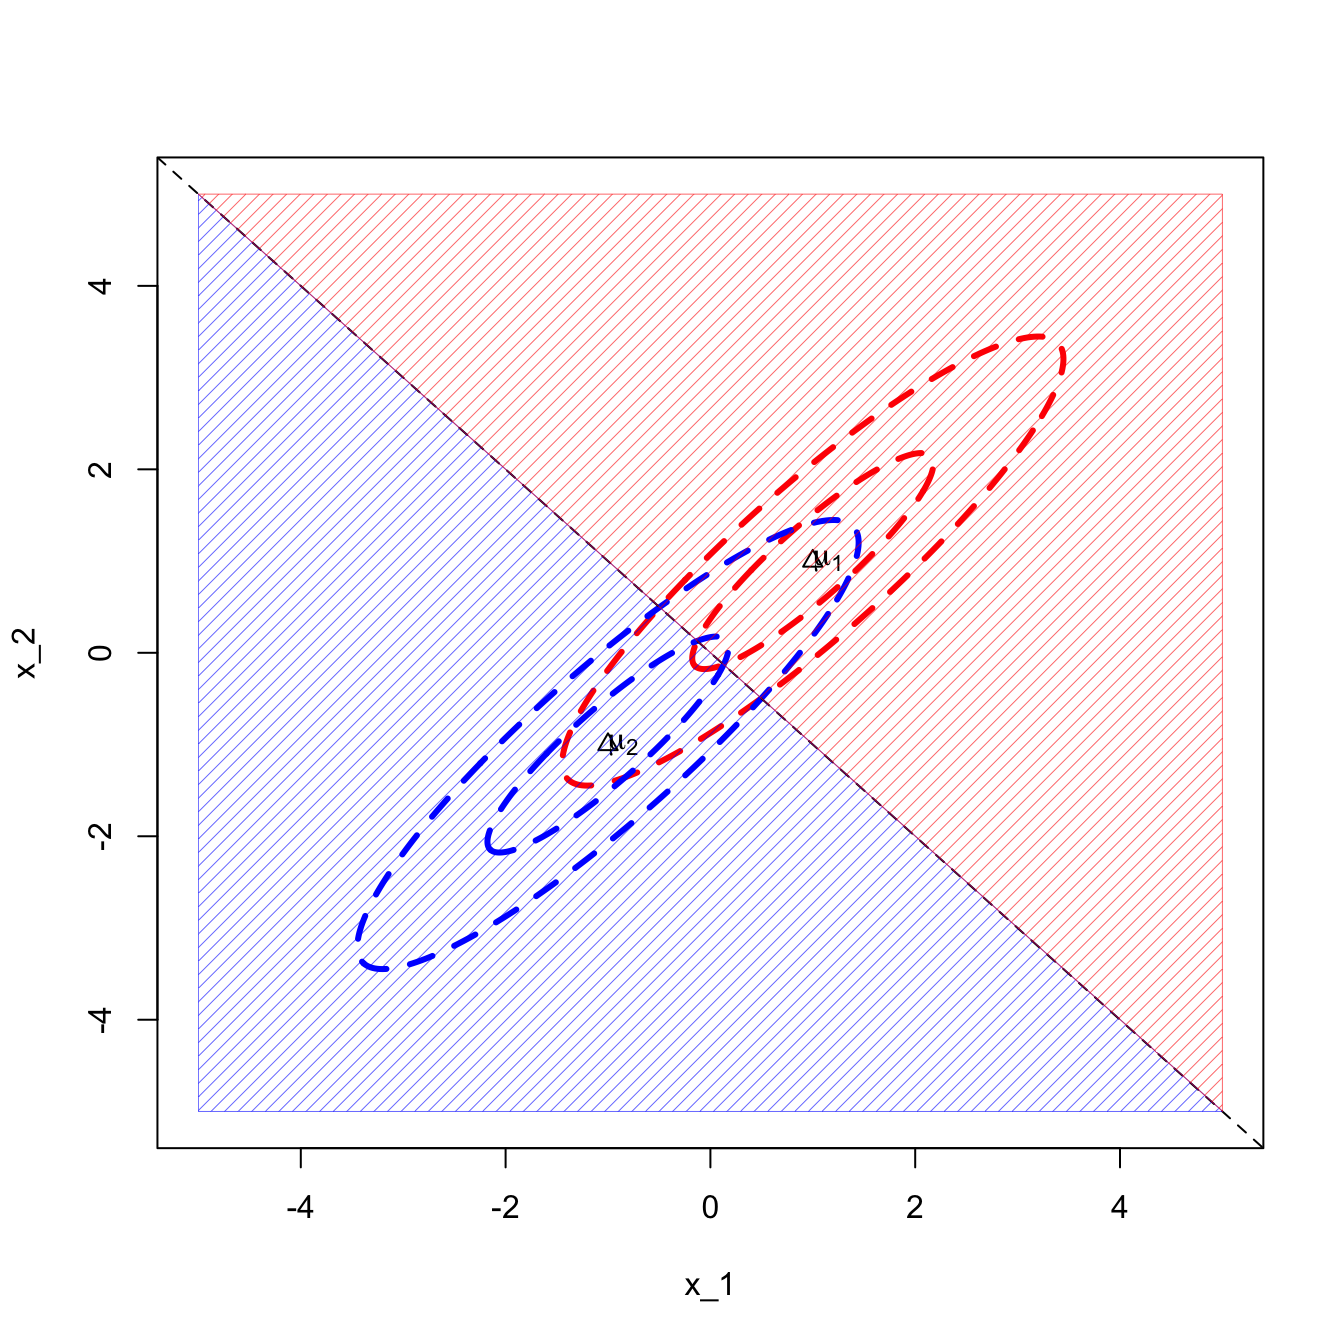
\includegraphics[width=1\linewidth]{03-matrix-decompositions_files/figure-latex/unnamed-chunk-4-1}

This is a \(512 \times 512\) colour image, meaning that there are three matrices \(\mathbf R, \mathbf B,\mathbf G\) of dimension \(512\times 512\)) giving the intensity of red, green, and blue for each pixel.
Naively storing this matrix requires 5.7Mb.

We can compute the SVD of the three colour intensity matrices, and the view the image that results from using reduced rank versions \(\mathbf B_k, \mathbf G_k, \mathbf R_k\) instead (as in Equation \eqref{eq:svdreduced}). The image below is formed using \(k=5, 30, 100\), and \(300\) basis vectors.

\begin{Shaded}
\begin{Highlighting}[]
\NormalTok{svd\_image }\OtherTok{\textless{}{-}} \ControlFlowTok{function}\NormalTok{(im,k)\{}
\NormalTok{  s }\OtherTok{\textless{}{-}} \FunctionTok{svd}\NormalTok{(im)}
\NormalTok{  Sigma\_k }\OtherTok{\textless{}{-}} \FunctionTok{diag}\NormalTok{(s}\SpecialCharTok{$}\NormalTok{d[}\DecValTok{1}\SpecialCharTok{:}\NormalTok{k])}
\NormalTok{  U\_k }\OtherTok{\textless{}{-}}\NormalTok{ s}\SpecialCharTok{$}\NormalTok{u[,}\DecValTok{1}\SpecialCharTok{:}\NormalTok{k]}
\NormalTok{  V\_k }\OtherTok{\textless{}{-}}\NormalTok{ s}\SpecialCharTok{$}\NormalTok{v[,}\DecValTok{1}\SpecialCharTok{:}\NormalTok{k]}
\NormalTok{  im\_k }\OtherTok{\textless{}{-}}\NormalTok{ U\_k }\SpecialCharTok{\%*\%}\NormalTok{ Sigma\_k }\SpecialCharTok{\%*\%} \FunctionTok{t}\NormalTok{(V\_k)}
   \DocumentationTok{\#\# the reduced rank SVD produces some intensities \textless{}0 and \textgreater{}1. }
  \CommentTok{\# Let\textquotesingle{}s truncate these}
\NormalTok{  im\_k[im\_k}\SpecialCharTok{\textgreater{}}\DecValTok{1}\NormalTok{]}\OtherTok{=}\DecValTok{1}
\NormalTok{  im\_k[im\_k}\SpecialCharTok{\textless{}}\DecValTok{0}\NormalTok{]}\OtherTok{=}\DecValTok{0}
  \FunctionTok{return}\NormalTok{(im\_k)}
\NormalTok{\}}

\FunctionTok{par}\NormalTok{(}\AttributeTok{mfrow=}\FunctionTok{c}\NormalTok{(}\DecValTok{2}\NormalTok{,}\DecValTok{2}\NormalTok{), }\AttributeTok{mar=}\FunctionTok{c}\NormalTok{(}\DecValTok{1}\NormalTok{,}\DecValTok{1}\NormalTok{,}\DecValTok{1}\NormalTok{,}\DecValTok{1}\NormalTok{))}

\NormalTok{pepprssvd}\OtherTok{\textless{}{-}}\NormalTok{ peppers}
\ControlFlowTok{for}\NormalTok{(k }\ControlFlowTok{in} \FunctionTok{c}\NormalTok{(}\DecValTok{4}\NormalTok{,}\DecValTok{30}\NormalTok{,}\DecValTok{100}\NormalTok{,}\DecValTok{300}\NormalTok{))\{}
\NormalTok{  svds}\OtherTok{\textless{}{-}}\FunctionTok{list}\NormalTok{()}
  \ControlFlowTok{for}\NormalTok{(ii }\ControlFlowTok{in} \DecValTok{1}\SpecialCharTok{:}\DecValTok{3}\NormalTok{) \{}
\NormalTok{    pepprssvd[,,ii]}\OtherTok{\textless{}{-}}\FunctionTok{svd\_image}\NormalTok{(peppers[,,ii],k)}
\NormalTok{  \}}
  \FunctionTok{plot}\NormalTok{(}\FunctionTok{as.raster}\NormalTok{(pepprssvd))}
\NormalTok{\}}
\end{Highlighting}
\end{Shaded}

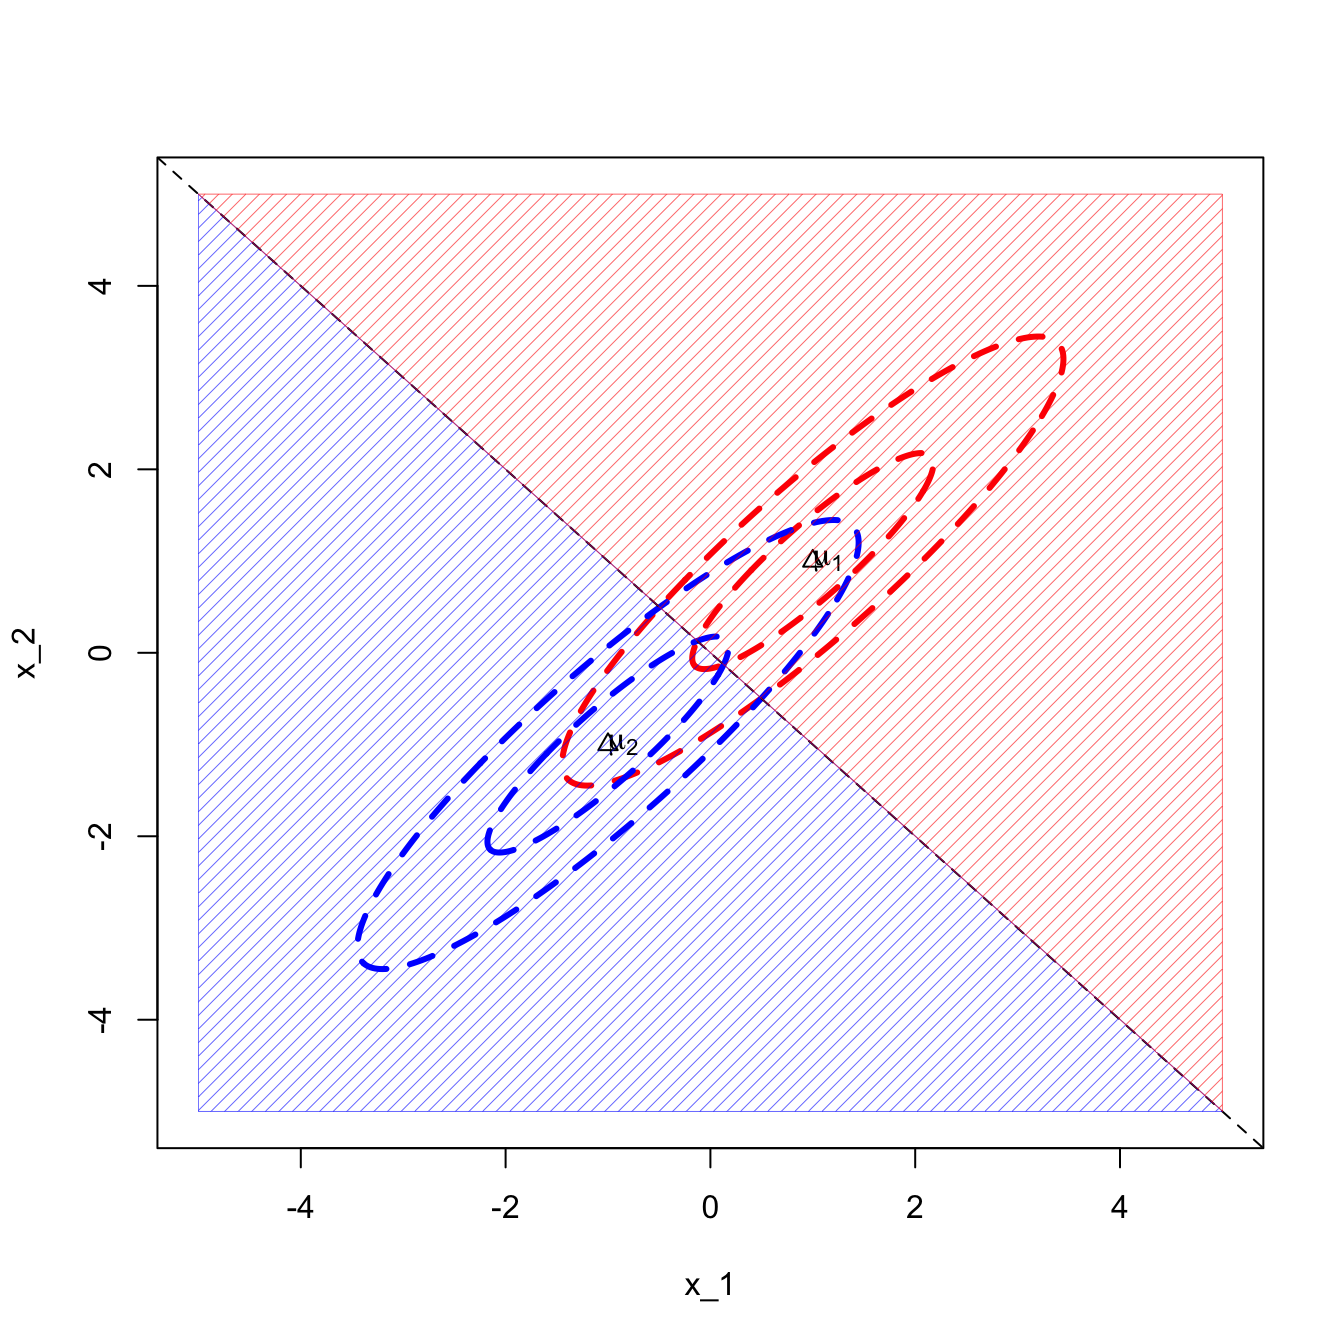
\includegraphics[width=1\linewidth]{03-matrix-decompositions_files/figure-latex/unnamed-chunk-5-1}

You can see that for \(k=30\) we have a reasonable approximation, but with some errors. With \(k=100\) it is hard to spot the difference with the original. The size of the four compressed images is 45Kb, 345Kb, 1.1Mb and 3.4Mb.

You can see further demonstrations of image compression with the SVD \href{http://timbaumann.info/svd-image-compression-demo/}{here}.

We will see much more of the SVD in later chapters.

\section{Computer tasks}\label{tasks-ch3}

\begin{enumerate}
\def\labelenumi{\arabic{enumi}.}
\tightlist
\item
  Finding the eigenvalues and eigenvectors of a matrix is easy in R.
\end{enumerate}

\begin{Shaded}
\begin{Highlighting}[]
\NormalTok{A}\OtherTok{=}\FunctionTok{matrix}\NormalTok{(}\FunctionTok{c}\NormalTok{(}\DecValTok{3}\NormalTok{,}\DecValTok{1}\NormalTok{,}\DecValTok{1}\NormalTok{,}\DecValTok{6}\NormalTok{),}\AttributeTok{nrow=}\DecValTok{2}\NormalTok{,}\AttributeTok{byrow=}\ConstantTok{TRUE}\NormalTok{)    }\CommentTok{\# use a to define a matrix A}
\NormalTok{Eig}\OtherTok{=}\FunctionTok{eigen}\NormalTok{(A)                     }\CommentTok{\# the eigenvalues and eigenvectors of A}
                                   \CommentTok{\# are stored in the list Eig}
\NormalTok{lambda}\OtherTok{=}\NormalTok{Eig}\SpecialCharTok{$}\NormalTok{values                }\CommentTok{\# extract the eigenvalues from Eig and}
                                   \CommentTok{\# store in the vector e}
\NormalTok{lambda                           }\CommentTok{\# you should see the eigenvalues in}
\end{Highlighting}
\end{Shaded}

\begin{verbatim}
## [1] 6.302776 2.697224
\end{verbatim}

\begin{Shaded}
\begin{Highlighting}[]
                                   \CommentTok{\# descending order}
\NormalTok{Q}\OtherTok{=}\NormalTok{Eig}\SpecialCharTok{$}\NormalTok{vectors                    }\CommentTok{\# extract the eigenvectors from Eig and}
                                   \CommentTok{\# store then in the columns of Q}
\end{Highlighting}
\end{Shaded}

The spectral decomposition of \(\mathbf A\) is
\[\mathbf A= \mathbf Q\boldsymbol \Lambda\mathbf Q^\top\]
Let's check this in R (noting as always that there may be some numerical errors)

\begin{Shaded}
\begin{Highlighting}[]
\NormalTok{Q}\SpecialCharTok{\%*\%}\FunctionTok{diag}\NormalTok{(lambda)}\SpecialCharTok{\%*\%}\FunctionTok{t}\NormalTok{(Q)          }\CommentTok{\# reconstruct A,}
\end{Highlighting}
\end{Shaded}

\begin{verbatim}
##      [,1] [,2]
## [1,]    3    1
## [2,]    1    6
\end{verbatim}

\begin{Shaded}
\begin{Highlighting}[]
                                   \CommentTok{\# where t(Q) gives the transpose of Q}
\end{Highlighting}
\end{Shaded}

Since A is positive definite, we can calculate the symmetric, positive definite square root of A.

\begin{Shaded}
\begin{Highlighting}[]
\NormalTok{Asqrt}\OtherTok{=}\NormalTok{Q}\SpecialCharTok{\%*\%}\FunctionTok{diag}\NormalTok{(lambda}\SpecialCharTok{**}\FloatTok{0.5}\NormalTok{)}\SpecialCharTok{\%*\%}\FunctionTok{t}\NormalTok{(Q) }\CommentTok{\# lambda**0.5 contains the square roots}
\NormalTok{Asqrt}\SpecialCharTok{\%*\%}\NormalTok{Asqrt                      }\CommentTok{\# it is seen that A is recovered}
\end{Highlighting}
\end{Shaded}

\begin{verbatim}
##      [,1] [,2]
## [1,]    3    1
## [2,]    1    6
\end{verbatim}

\begin{itemize}
\tightlist
\item
  Instead of using the full eigendecomposition for \(\mathbf A\), try truncating it and using just a single eigenvalue and eigenvector, i.e., compute
  \[\mathbf A' = \lambda_1 \mathbf q_1 \mathbf q_1^\top\]
\item
  Compute the difference between \(\mathbf A\) and \(\mathbf A'\) using the 2-norm and the Frobenius norm.
\end{itemize}

\begin{enumerate}
\def\labelenumi{\arabic{enumi}.}
\setcounter{enumi}{1}
\tightlist
\item
  The singular value decomposition can be computed in R using the command \texttt{svd}. Let \(\mathbf X\) be the four numerical variables in the \texttt{iris} dataset with the column mean removed
\end{enumerate}

\begin{Shaded}
\begin{Highlighting}[]
\NormalTok{n}\OtherTok{=}\DecValTok{150}
\NormalTok{H}\OtherTok{=}\FunctionTok{diag}\NormalTok{(}\FunctionTok{rep}\NormalTok{(}\DecValTok{1}\NormalTok{,n))}\SpecialCharTok{{-}}\FunctionTok{rep}\NormalTok{(}\DecValTok{1}\NormalTok{,n)}\SpecialCharTok{\%*\%}\FunctionTok{t}\NormalTok{(}\FunctionTok{rep}\NormalTok{(}\DecValTok{1}\NormalTok{,n))}\SpecialCharTok{/}\NormalTok{n   }\CommentTok{\# calculate the centering matrix H}
\NormalTok{X}\OtherTok{=}\NormalTok{H}\SpecialCharTok{\%*\%} \FunctionTok{as.matrix}\NormalTok{(iris[,}\DecValTok{1}\SpecialCharTok{:}\DecValTok{4}\NormalTok{])}
\CommentTok{\# This can also be done using the command}
\CommentTok{\# sweep(iris[,1:4], 2, colMeans(iris[,1:4]))  \# do you understand why?}
\end{Highlighting}
\end{Shaded}

\begin{itemize}
\item
  Compute the SVD of \(\mathbf X\) in R and report its singular values.
\item
  Does R report the full or compact SVD?
\item
  Check that \(\mathbf X\mathbf v= \sigma \mathbf u\).
\item
  Compute the best rank-1, rank-2, and rank-3 approximations to \(\mathbf X\), and report the 2-norm and Frobenious norm for these approximations
\item
  Compute the eigenvalues of \(\mathbf X^\top \mathbf X\). How do these relate to the singular values? How does \(\mathbf X^\top \mathbf X\) relate to the sample covariance matrix of the iris data? How do the singular values relate to the eigenvalues of the covariance matrix?
\item
  Let \(\mathbf S\) be the sample covariance matrix of the iris dataset. What vector \(\mathbf x\) with \(||\mathbf x||=1\) maximizes \(\mathbf x^\top \mathbf S\mathbf x\)?
\end{itemize}

\begin{enumerate}
\def\labelenumi{\arabic{enumi}.}
\setcounter{enumi}{2}
\item
  Choose an few images from the \href{http://sipi.usc.edu/database/}{USC-SIPI Image Database} and repeat the image compression example from the notes. Which type of images compress well do you think?
\item
  We won't discuss how the SVD is computed in practice, but there are a variety of approaches that can be used. Try the following iterative approach for computing the first singular vectors:
\end{enumerate}

\begin{Shaded}
\begin{Highlighting}[]
\NormalTok{X }\OtherTok{\textless{}{-}} \FunctionTok{as.matrix}\NormalTok{(iris[,}\DecValTok{1}\SpecialCharTok{:}\DecValTok{4}\NormalTok{])}
\NormalTok{v }\OtherTok{\textless{}{-}} \FunctionTok{rnorm}\NormalTok{(}\FunctionTok{dim}\NormalTok{(X)[}\DecValTok{2}\NormalTok{])}

\ControlFlowTok{for}\NormalTok{ (iter }\ControlFlowTok{in} \DecValTok{1}\SpecialCharTok{:}\DecValTok{500}\NormalTok{)\{}
\NormalTok{  u }\OtherTok{\textless{}{-}}\NormalTok{ X }\SpecialCharTok{\%*\%}\NormalTok{v}
\NormalTok{  u }\OtherTok{\textless{}{-}}\NormalTok{ u}\SpecialCharTok{/}\FunctionTok{sqrt}\NormalTok{(}\FunctionTok{sum}\NormalTok{(u}\SpecialCharTok{\^{}}\DecValTok{2}\NormalTok{)) }
\NormalTok{  v }\OtherTok{\textless{}{-}} \FunctionTok{t}\NormalTok{(X) }\SpecialCharTok{\%*\%}\NormalTok{u}
\NormalTok{  v }\OtherTok{\textless{}{-}}\NormalTok{ v}\SpecialCharTok{/}\FunctionTok{sqrt}\NormalTok{(}\FunctionTok{sum}\NormalTok{(v}\SpecialCharTok{\^{}}\DecValTok{2}\NormalTok{)) }
\NormalTok{\}}
\NormalTok{X.svd }\OtherTok{\textless{}{-}} \FunctionTok{svd}\NormalTok{(X)}
\NormalTok{X.svd}\SpecialCharTok{$}\NormalTok{v[,}\DecValTok{1}\NormalTok{]}\SpecialCharTok{/}\NormalTok{v}
\NormalTok{X.svd}\SpecialCharTok{$}\NormalTok{u[,}\DecValTok{1}\NormalTok{]}\SpecialCharTok{/}\NormalTok{u}
\end{Highlighting}
\end{Shaded}

\section{Exercises}\label{exercises-ch3}

\begin{enumerate}
\def\labelenumi{\arabic{enumi}.}
\setcounter{enumi}{-1}
\item
  There is a great Twitter thread on the SVD by Daniella Witten. Read it \href{https://twitter.com/WomenInStat/status/1285610321747611653}{here}.
\item
  Let \(\boldsymbol{\Sigma}\) be an arbitrary covariance matrix.

  \begin{itemize}
  \tightlist
  \item
    Show \(\boldsymbol{\Sigma}\) is symmetric and
    positive semi-definite.
  \item
    Give examples of both singular and non-singular covariance matrices.\\
  \item
    What condition must the eigenvalues of a non-singular covariance matrix satisfy?
  \end{itemize}
\end{enumerate}

\begin{enumerate}
\def\labelenumi{\arabic{enumi}.}
\setcounter{enumi}{1}
\tightlist
\item
  Compute, by hand (but check your answer in R), the singular value decomposition (full and compact) of the following matrices.

  \begin{itemize}
  \tightlist
  \item
    \(\left(\begin{array}{cc}2&0\\0&-1\end{array}
    \right)\)
  \item
    \(\left(\begin{array}{cc}1&0\\0&0\\0&0\end{array}
    \right)\)
  \end{itemize}
\item
  Let \[\mathbf X=\left(\begin{array}{cc}1&1\\0&1\\1&0\end{array}
  \right)\]\\
  The eigen-decomposition of \(\mathbf X^\top \mathbf X\) is
  \[\mathbf X^\top \mathbf X=\frac{1}{\sqrt{2}}\left(\begin{array}{cc}1&-1\\1&1\end{array}
  \right) \left(\begin{array}{cc}3&0\\0&1\end{array}
  \right)\frac{1}{\sqrt{2}}\left(\begin{array}{cc}1&-1\\1&1\end{array}
  \right)^\top \]
  Use this fact to compute answer the following questions:

  \begin{itemize}
  \tightlist
  \item
    What are the singular values of \(\mathbf X\)?
  \item
    What are the right singular vectors of \(\mathbf X\)?
  \item
    What are the left singular vectors of \(\mathbf X\)?
  \item
    Give the compact SVD of \(\mathbf X\). Check your answer, noting that the singular vectors are only specified up to multiplication by \(-1\)
  \item
    Can you compute the full SVD of \(\mathbf X\)?
  \item
    What is the eigen-decomposition of \(\mathbf X\mathbf X^\top\)?
  \item
    Find a generalised inverse of matrix \(\mathbf X\).
  \end{itemize}
\end{enumerate}

\begin{enumerate}
\def\labelenumi{\arabic{enumi}.}
\setcounter{enumi}{3}
\item
  The SVD can be used to solve linear systems of the form
  \[\mathbf A\mathbf x= \mathbf y\]
  where \(\mathbf A\) is a \(n\times p\) matrix, with compact SVD
  \(\mathbf A= \mathbf U\boldsymbol{\Sigma}\mathbf V^\top\).

  \begin{itemize}
  \item
    If \(\mathbf A\) is a square invertible matrix, show that \[\tilde{\mathbf x} = \mathbf V\boldsymbol{\Sigma}^{-1} \mathbf U^\top \mathbf y\] is the unique solution to \(\mathbf A\mathbf x= \mathbf y\), i.e., show that \(\mathbf A^{-1} =  \mathbf V\boldsymbol{\Sigma}^{-1} \mathbf U^\top\).
  \item
    If \(\mathbf A\) is not a square matrix, then \(\mathbf A^+ = \mathbf V\boldsymbol{\Sigma}^{-1} \mathbf U^\top\) is a generalized inverse (not a true inverse) matrix, and
    \(\tilde{\mathbf x}=\mathbf A^+\mathbf y\) is still a useful quantity to consider as we shall now see. Let \(\mathbf A=\left(\begin{array}{cc}1&1\\0&1\\1&0\end{array}
    \right)\) and \(\mathbf y= \left(\begin{array}{c}2\\1\\1\end{array}
    \right)\). Then \(\mathbf A\mathbf x=\mathbf y\) is an over-determined system in that there are 3 equations in 2 unknowns. Compute \(\tilde{\mathbf x}=\mathbf A^+\mathbf y\). Is this a solution to the equation?
  \end{itemize}

  \textbf{Note} that you computed the svd for \(\mathbf A\) in Q2.

  \begin{itemize}
  \tightlist
  \item
    Now suppose \(\mathbf y= \left(\begin{array}{c}1\\-1\\1\end{array}
    \right)\). There is no solution to \(\mathbf A\mathbf x=\mathbf y\) in this case as \(\mathbf y\) is not in the column space of \(\mathbf A\). Prove that \({\tilde{\mathbf x}} = \mathbf A^+\mathbf y\) solves the least squares problem
    \[\tilde{\mathbf x} = \arg\min_{\mathbf x}||\mathbf y- \mathbf A\mathbf x||_2.\]
  \end{itemize}

  \textbf{Hint}: You can either do this directly for this problem, or you can show that the least squares solution \((\mathbf A^\top \mathbf A)^{-1}\mathbf A^\top \mathbf y=\tilde{\mathbf x}\).
\item
  Consider the system
  \[\mathbf B\mathbf x= \mathbf y\mbox{ with }\mathbf B=\left(\begin{array}{ccc}1&0&1\\1&1&0\end{array}
  \right),\mathbf y= \left(\begin{array}{c}1\\1\end{array}
  \right).\]
  This is an underdetermined system, as there are 2 equations in 3 unknowns, and so there are an infinite number of solutions for \(\mathbf x\) in this case.

  \begin{itemize}
  \tightlist
  \item
    Find the full SVD for \(\mathbf B=\mathbf U\boldsymbol{\Sigma}\mathbf V^\top\) (noting that \(\mathbf B=\mathbf A^\top\) for \(\mathbf A\) from the previous question).
  \item
    Compute
    \(\tilde{\mathbf x}=\mathbf B^+\mathbf y\), check it is a solution to the equation, and explain why \[\tilde{\mathbf x}= \sum_{i=1}^r \mathbf v_i \frac{\mathbf u_i^\top \mathbf y}{\sigma_i}\] in general, where \(r\leq max(n,p)\) is the rank of \(\mathbf B\), and write out \(\tilde{\mathbf x}\) explicitly in this form for the given \(\mathbf B\).
  \item
    Consider \(\mathbf x\) of the form
    \[\mathbf x= \tilde{\mathbf x} + \sum_{i=r+1}^p \alpha_i \mathbf v_i\]
    and explain why any \(\mathbf x\) of this form is also a solution to \(\mathbf B\mathbf x=\mathbf y\). Thus write out all possible solutions of the equation.
  \item
    Prove that \(\tilde{\mathbf x}\) is the solution with minimum norm, i.e., \(||\tilde{\mathbf x}||_2 \leq ||\mathbf x||_2\). \textbf{Hint} \(\mathbf v_1, \ldots, \mathbf v_p\) form a complete orthonormal basis for \(\mathbb{R}^p\).
  \end{itemize}
\item
  Prove proposition \ref{prp:eigproj}, namely that the eigenvalues of projection matrices are either 0 or 1.
  Show that \({\bf 1}_n\) is an eigenvector of \(\mathbf H\). What is the corresponding eigenvalue? What are the remaining eigenvalues equal to?
\end{enumerate}

\chapter*{PART II: Dimension reduction methods}\label{part-ii-dimension-reduction-methods}
\addcontentsline{toc}{chapter}{PART II: Dimension reduction methods}

\href{https://mediaspace.nottingham.ac.uk/media/Part+IIA+Dimension+reduction+introduction/1_0s2cgr1r}{Introductory Video}

In many applications, a large number of variables are recorded for each experimental unit under study. For example, if we think of individual people as the \emph{experimental units}, then in a health check-up we might collect data on age, blood pressure, cholesterol level, blood test results, lung function, weight, height, BMI, etc. If you use websites such as Amazon, Facebook, and Google, they store thousands (possibly millions) of pieces of information about you (\href{https://www.theguardian.com/commentisfree/2018/mar/28/all-the-data-facebook-google-has-on-you-privacy}{this article} shows you how to download the information Google stores about you, including all the locations you've visited, every search, youtube video, or app you've used and more). They process this data to create an individual profile for each user, which they can then use to create targetted adverts.

When analysing data of moderate or high dimension, it is often desirable to seeks ways to restructure the data and reduce its dimension whilst \textbf{retaining the most important information} within the data or \textbf{preserving some feature of interest} in the data. There a variety of reasons we might want to do this.

\begin{itemize}
\tightlist
\item
  In reduced dimensions, it is often much easier to understand and appreciate the most important features of a dataset.
\item
  If there is a lot of reduncancy in the data, we might want to reduce the dimension to lower the memory requirements in storing it (e.g.~with sound and image compression).
\item
  In high dimensions, it can be difficult to analyse data (e.g.~with statistical methods), and so reducing the dimension can be a way to make a dataset amenable to analysis.
\end{itemize}

In this part of the module we investigate three different methods for dimension reduction: Principal Component Analysis (PCA) in Chapter \ref{pca}; Canonical Correlation Analysis (CCA) in Chapter \ref{cca}; and Multidimensional Scaling (MDS) in Chapter \ref{mds}. Matrix algebra (Chapters \ref{linalg-prelim} and \ref{linalg-decomp}) plays a key role in all three of these techniques.

\subsection*{A warning}\label{a-warning}
\addcontentsline{toc}{subsection}{A warning}

Beware that high-dimensional data can behave qualitatively differently to low-dimensional data. As an example, lets consider 1000 points uniformly distributed in \([0,1]^d\), and think about how close together or spread out the points are. A simple way to do this is to consider the ratio of the maximum and minimum distance between any two points in our sample.

\begin{Shaded}
\begin{Highlighting}[]
\NormalTok{N}\OtherTok{\textless{}{-}}\DecValTok{1000}
\NormalTok{averatio }\OtherTok{\textless{}{-}}\FunctionTok{c}\NormalTok{()}
\NormalTok{ii}\OtherTok{\textless{}{-}}\DecValTok{1}
\ControlFlowTok{for}\NormalTok{(d }\ControlFlowTok{in} \FunctionTok{c}\NormalTok{(}\DecValTok{2}\NormalTok{,}\DecValTok{5}\NormalTok{,}\DecValTok{10}\NormalTok{,}\DecValTok{20}\NormalTok{,}\DecValTok{30}\NormalTok{,}\DecValTok{40}\NormalTok{,}\DecValTok{50}\NormalTok{,}\DecValTok{60}\NormalTok{,}\DecValTok{80}\NormalTok{,}\DecValTok{100}\NormalTok{, }\DecValTok{200}\NormalTok{, }\DecValTok{350}\NormalTok{, }\DecValTok{500}\NormalTok{, }\DecValTok{750}\NormalTok{, }\DecValTok{1000}\NormalTok{))\{}
\NormalTok{  averatio[ii] }\OtherTok{\textless{}{-}} \FunctionTok{mean}\NormalTok{(}\FunctionTok{replicate}\NormalTok{(}\DecValTok{10}\NormalTok{, \{}
\NormalTok{  X}\OtherTok{\textless{}{-}}\FunctionTok{matrix}\NormalTok{(}\FunctionTok{runif}\NormalTok{(N}\SpecialCharTok{*}\NormalTok{d), }\AttributeTok{nc=}\NormalTok{d)}
\NormalTok{  d }\OtherTok{\textless{}{-}} \FunctionTok{as.matrix}\NormalTok{(}\FunctionTok{dist}\NormalTok{(X)) }
  \CommentTok{\# this gives a N x N matrix of the Euclidean distances between the data points.}
\NormalTok{  maxdist }\OtherTok{\textless{}{-}} \FunctionTok{max}\NormalTok{(d) }
\NormalTok{  mindist }\OtherTok{\textless{}{-}} \FunctionTok{min}\NormalTok{(d}\SpecialCharTok{+}\FunctionTok{diag}\NormalTok{(}\DecValTok{10}\SpecialCharTok{\^{}}\DecValTok{5}\NormalTok{, }\AttributeTok{nrow=}\NormalTok{N)) }
  \CommentTok{\# The diagonal elements of the distance matrix are zero,}
  \CommentTok{\# so I\textquotesingle{}ve added a big number to the diagonal }
  \CommentTok{\# so that we get the minimum distance between different points}
\NormalTok{  maxdist}\SpecialCharTok{/}\NormalTok{mindist\}))}
\NormalTok{  ii }\OtherTok{\textless{}{-}}\NormalTok{ ii}\SpecialCharTok{+}\DecValTok{1}
\NormalTok{\}}
\FunctionTok{plot}\NormalTok{(}\FunctionTok{c}\NormalTok{(}\DecValTok{2}\NormalTok{,}\DecValTok{5}\NormalTok{,}\DecValTok{10}\NormalTok{,}\DecValTok{20}\NormalTok{,}\DecValTok{30}\NormalTok{,}\DecValTok{40}\NormalTok{,}\DecValTok{50}\NormalTok{,}\DecValTok{60}\NormalTok{,}\DecValTok{80}\NormalTok{,}\DecValTok{100}\NormalTok{, }\DecValTok{200}\NormalTok{, }\DecValTok{350}\NormalTok{, }\DecValTok{500}\NormalTok{, }\DecValTok{750}\NormalTok{, }\DecValTok{1000}\NormalTok{), }
\NormalTok{     averatio, }\AttributeTok{ylab=}\StringTok{\textquotesingle{}Max. dist. / min. dist.\textquotesingle{}}\NormalTok{, }\AttributeTok{xlab=}\StringTok{\textquotesingle{}Dimension d\textquotesingle{}}\NormalTok{, }\AttributeTok{log=}\StringTok{\textquotesingle{}xy\textquotesingle{}}\NormalTok{)}
\end{Highlighting}
\end{Shaded}

\includegraphics{04-pca_files/figure-latex/unnamed-chunk-1-1.pdf}

So we can see that as the dimension increases, the ratio of the maximum and minimum distance between any two random points in our sample tends to 1. In other words, all points are the same distance apart!

\chapter{Principal Component Analysis (PCA)}\label{pca}

The videos for this chapter are available at the following links:

\begin{itemize}
\tightlist
\item
  \href{https://mediaspace.nottingham.ac.uk/media/PCA_Informal/1_zs9dumou}{4.1 An informal introduction to PCA}
\item
  \href{https://mediaspace.nottingham.ac.uk/media/PCA+Informal+Examples/1_3c9ghrtf}{4.1.5 Informal Examples}
\item
  \href{https://mediaspace.nottingham.ac.uk/media/PCA+Formal+Description/1_tq8tpcn0}{4.2 A more formal description of PCA}
\item
  \href{https://mediaspace.nottingham.ac.uk/media/PCAA+Properties+\%28edited\%29/1_vax8yhp9}{4.2.1 Properties of PC scores}
\item
  \href{https://mediaspace.nottingham.ac.uk/media/PCA+Football+Example/1_h70vgqq2}{4.2.2 Example: PCA of the football data}
\item
  \href{https://mediaspace.nottingham.ac.uk/media/Population+PCA+and+transformations/1_y1s2arei}{4.2.4 Population PCA and transformations}
\item
  \href{https://mediaspace.nottingham.ac.uk/media/PCAA+Minimizing+Reconstruction+Error/1_93tzf0ju}{4.3 An alternative view of PCA: minimizing reconstruction error`}
\item
  \href{https://mediaspace.nottingham.ac.uk/media/PCAA+MNIST+example/1_ljte3zc1}{4.3.1 Example: PCA of the MNIST data}
\end{itemize}

With multivariate data, it is common to want to reduce the dimension of the data \emph{in a sensible way}. For example

\begin{itemize}
\item
  exam marks across different modules are
  averaged to produce a single overall mark for each
  student
\item
  a football league table converts the
  numbers of wins, draws and losses to a single measure of
  points.
\end{itemize}

Mathematically, these summaries
are both linear combinations of the
original variables of the form
\[y = \mathbf u^\top \mathbf x.\]\\
for some choice of \(\mathbf u\).

For the exam marks example, suppose each student sits \(p=4\) modules
with marks, \(x_1,x_2,x_3,x_4\). Then, writing \(\mathbf x=(x_1, x_2 , x_3, x_4)^\top\) and choosing \(\mathbf u= \left(\frac{1}{4}, \frac{1}{4}, \frac{1}{4}, \frac{1}{4} \right)^\top\)
gives an overall average,
\[ y =\mathbf u^\top \mathbf x= \begin{pmatrix} \frac{1}{4} & \frac{1}{4} & \frac{1}{4} & \frac{1}{4} \end{pmatrix} \begin{pmatrix} x_1 \\ x_2 \\ x_3 \\ x_4 \end{pmatrix} = \frac{x_1}{4} + \frac{x_2}{4} + \frac{x_3}{4} + \frac{x_4}{4}.\]

For the football league table, if \(w\) is the number of wins, \(d\) is the number of draws and \(l\) is the number of losses then, writing
\({\mathbf r}=(w,d,l)^\top\), we choose \(\mathbf u= \left(3,1,0 \right)^\top\) to get the points score
\[ y = \mathbf u^\top {\mathbf r}=\begin{pmatrix} 3 & 1 & 0 \end{pmatrix} \begin{pmatrix} w \\ d \\ l \end{pmatrix} = 3w + 1d + 0l=3w+d.\]

\subsubsection*{Geometric interpretation}\label{geometric-interpretation}
\addcontentsline{toc}{subsubsection}{Geometric interpretation}

In the two examples above, we used the vector \(\mathbf u\) to convert our original variables, \(\mathbf x\),
to a new variable, \(y\), by projecting \(\mathbf x\) onto \(\mathbf u\).
We can think of this as a projection onto the subspace defined by \(\mathbf u\)

\[U = \operatorname{span}\{\mathbf u\} = \{\lambda \mathbf u: \lambda \in \mathbb{R}\}\subset \mathbb{R}^p,\]

For the exam data, each data point \(\mathbf x= \begin{pmatrix} x_1 \\ x_2 \\ x_3 \\ x_4 \end{pmatrix}\)
is a vector in \(\mathbb{R}^4\), and we've expressed \(\mathbf x\) in terms of its coordinates with respsect to the standard basis, \(\mathbf e_1^\top = (1\; 0\; 0 \; 0)\) etc:
\[\mathbf x=x_1 \mathbf e_1 + x_2 \mathbf e_2 +x_3 \mathbf e_3 +x_4 \mathbf e_4.\]
The vector subspace \(U\) is a line in \(\mathbb{R}^4\) along the direction \(\mathbf u= \begin{pmatrix} \frac{1}{4} & \frac{1}{4} & \frac{1}{4} & \frac{1}{4} \end{pmatrix}^\top\).

How do we project onto subspace \(U\)?

\begin{itemize}
\tightlist
\item
  If \(||\mathbf u||_2=1\) then the orthogonal projection of \(\mathbf x\) onto \(U\) is\\
  \[\mathbf u\mathbf u^\top\mathbf x.\]
  Or in other words, the projection of \(\mathbf x\) onto subspace \(U\) has coordinate \(\mathbf u^\top \mathbf x\) with respect to basis \(\{\mathbf u\}\).
\end{itemize}

If you prefer to think in terms of projection matrices (see Chapter \ref{orthogproj}), then the matrix for projecting onto \(U\) is
\[\mathbf P_U = \mathbf u(\mathbf u^\top \mathbf u)^{-1}\mathbf u^\top\]
which simplifies to
\[\mathbf P_U = \mathbf u\mathbf u^\top\]
when \(||\mathbf u||=\sqrt{\mathbf u^\top\mathbf u}=1\) so that we again see the projection of \(\mathbf x\) onto \(U\) is \(y=\mathbf P_u \mathbf x= \mathbf u\mathbf u^\top\mathbf x\).

\textbf{How should we choose \(\mathbf u\)?}

The answer to that question depends upon the goal of the analysis. For the exam and football league examples, the choice of \(\mathbf u\) is an arbitrary decision taken in order to reduce a multidimensional dataset to a single variable (average mark, or points).

A single \(\mathbf u\) gives a \textbf{snapshot} or summary of the data. If \(\mathbf u\) is chosen well that snapshot may tell us much of what we want to know about the data, e.g.,

\begin{itemize}
\tightlist
\item
  Liverpool won the league,
\item
  student \(X\)'s exam performance was first class etc.
\end{itemize}

In many cases we will want to use multiple snapshots: instead of using a single \(\mathbf u\), we will use a collection \(\mathbf u_1, \mathbf u_2, \ldots, \mathbf u_r\) and consider the derived variables

\[\mathbf y= \begin{pmatrix} y_1\\y_2 \\ \vdots \\ y_r\end{pmatrix} = \begin{pmatrix}
\mathbf u_1^\top \mathbf x\\  \mathbf u_2^\top \mathbf x\\\vdots\\  \mathbf u_r^\top \mathbf x\end{pmatrix}\]

In matrix notation, if we set
\[\mathbf U= \begin{pmatrix} 
|&&|\\
\mathbf u_1 & \ldots & \mathbf u_r\\
|&&|\end{pmatrix}\]
then the new derived variable is
\[\mathbf y= \mathbf U^\top \mathbf x.\]

If \(\dim(\mathbf y)=r<p=\dim(\mathbf x)\) then we have reduced the dimension of the data. If \(\mathbf y\) tells us all we need to know about the data, then we can work (plot, analyse, model) with \(\mathbf y\) instead of \(\mathbf x\). If \(r\ll p\) this can make working with the data significantly easier, as we can more easily visulise and understand low dimensional problems.

We will study a variety of methods for choosing \(\mathbf U\). The methods can all be expressed as constrained optimization problems:

\begin{align}
\mbox{minimize} f_{\mathbf X}(\mathbf U) \label{eq:dimredopt} \\
\mbox{ subject to } \mathbf U\in \mathcal{U} 
\end{align}

The objective \(f_{\mathbf X}(\mathbf U)\) varies between methods: principal component analysis (PCA) maximizes variance or minimizes reconstruction error; canonical correlation analysis (CCA) maximizes correlation; multidimensional scaling (MDS) maximizes spread etc.

The contstraint on the search space \(\mathcal{U}\), is usually that \(\mathbf U\) must be (partially) orthogonal, but in other methods other constraints are used

\section{PCA: an informal introduction}\label{pca-an-informal-introduction}

There are two different ways of motivating
principal component analysis (PCA), which may in part explain why PCA is so widely used.

The first motivation, and the topic of this section, is to introduce PCA as method for maximizing the variance of the transformed variables \(\mathbf y\). We start by choosing \(\mathbf u_1\) so that \(y_1=\mathbf u_1^\top \mathbf x\) has maximum variance. We then choose \(\mathbf u_2\) so that \(y_2=\mathbf u_2^\top \mathbf x\) has maximum variance subject to being uncorrelated with \(y_1\), and so on.

The idea is to produce a set of variables \(y_1, y_2, \ldots, y_r\) that are uncorrelated, but which are most informative about the data. The thinking is that if a variable has large variance it must be informative/important.

The name \textbf{principal component analysis} comes from thinking of this as splitting the data \(\mathbf X\) into its most important parts. It therefore won't surprise you to find that this involves the matrix decompositions we studied in Chapter \ref{linalg-decomp}.

\href{https://twitter.com/allison_horst/status/1288904459490213888?lang=en}{Allison Horst (@allison\_horst)} gave a great illustration of how to think about PCA on Twitter. Imagine you are a whale shark with a wide mouth

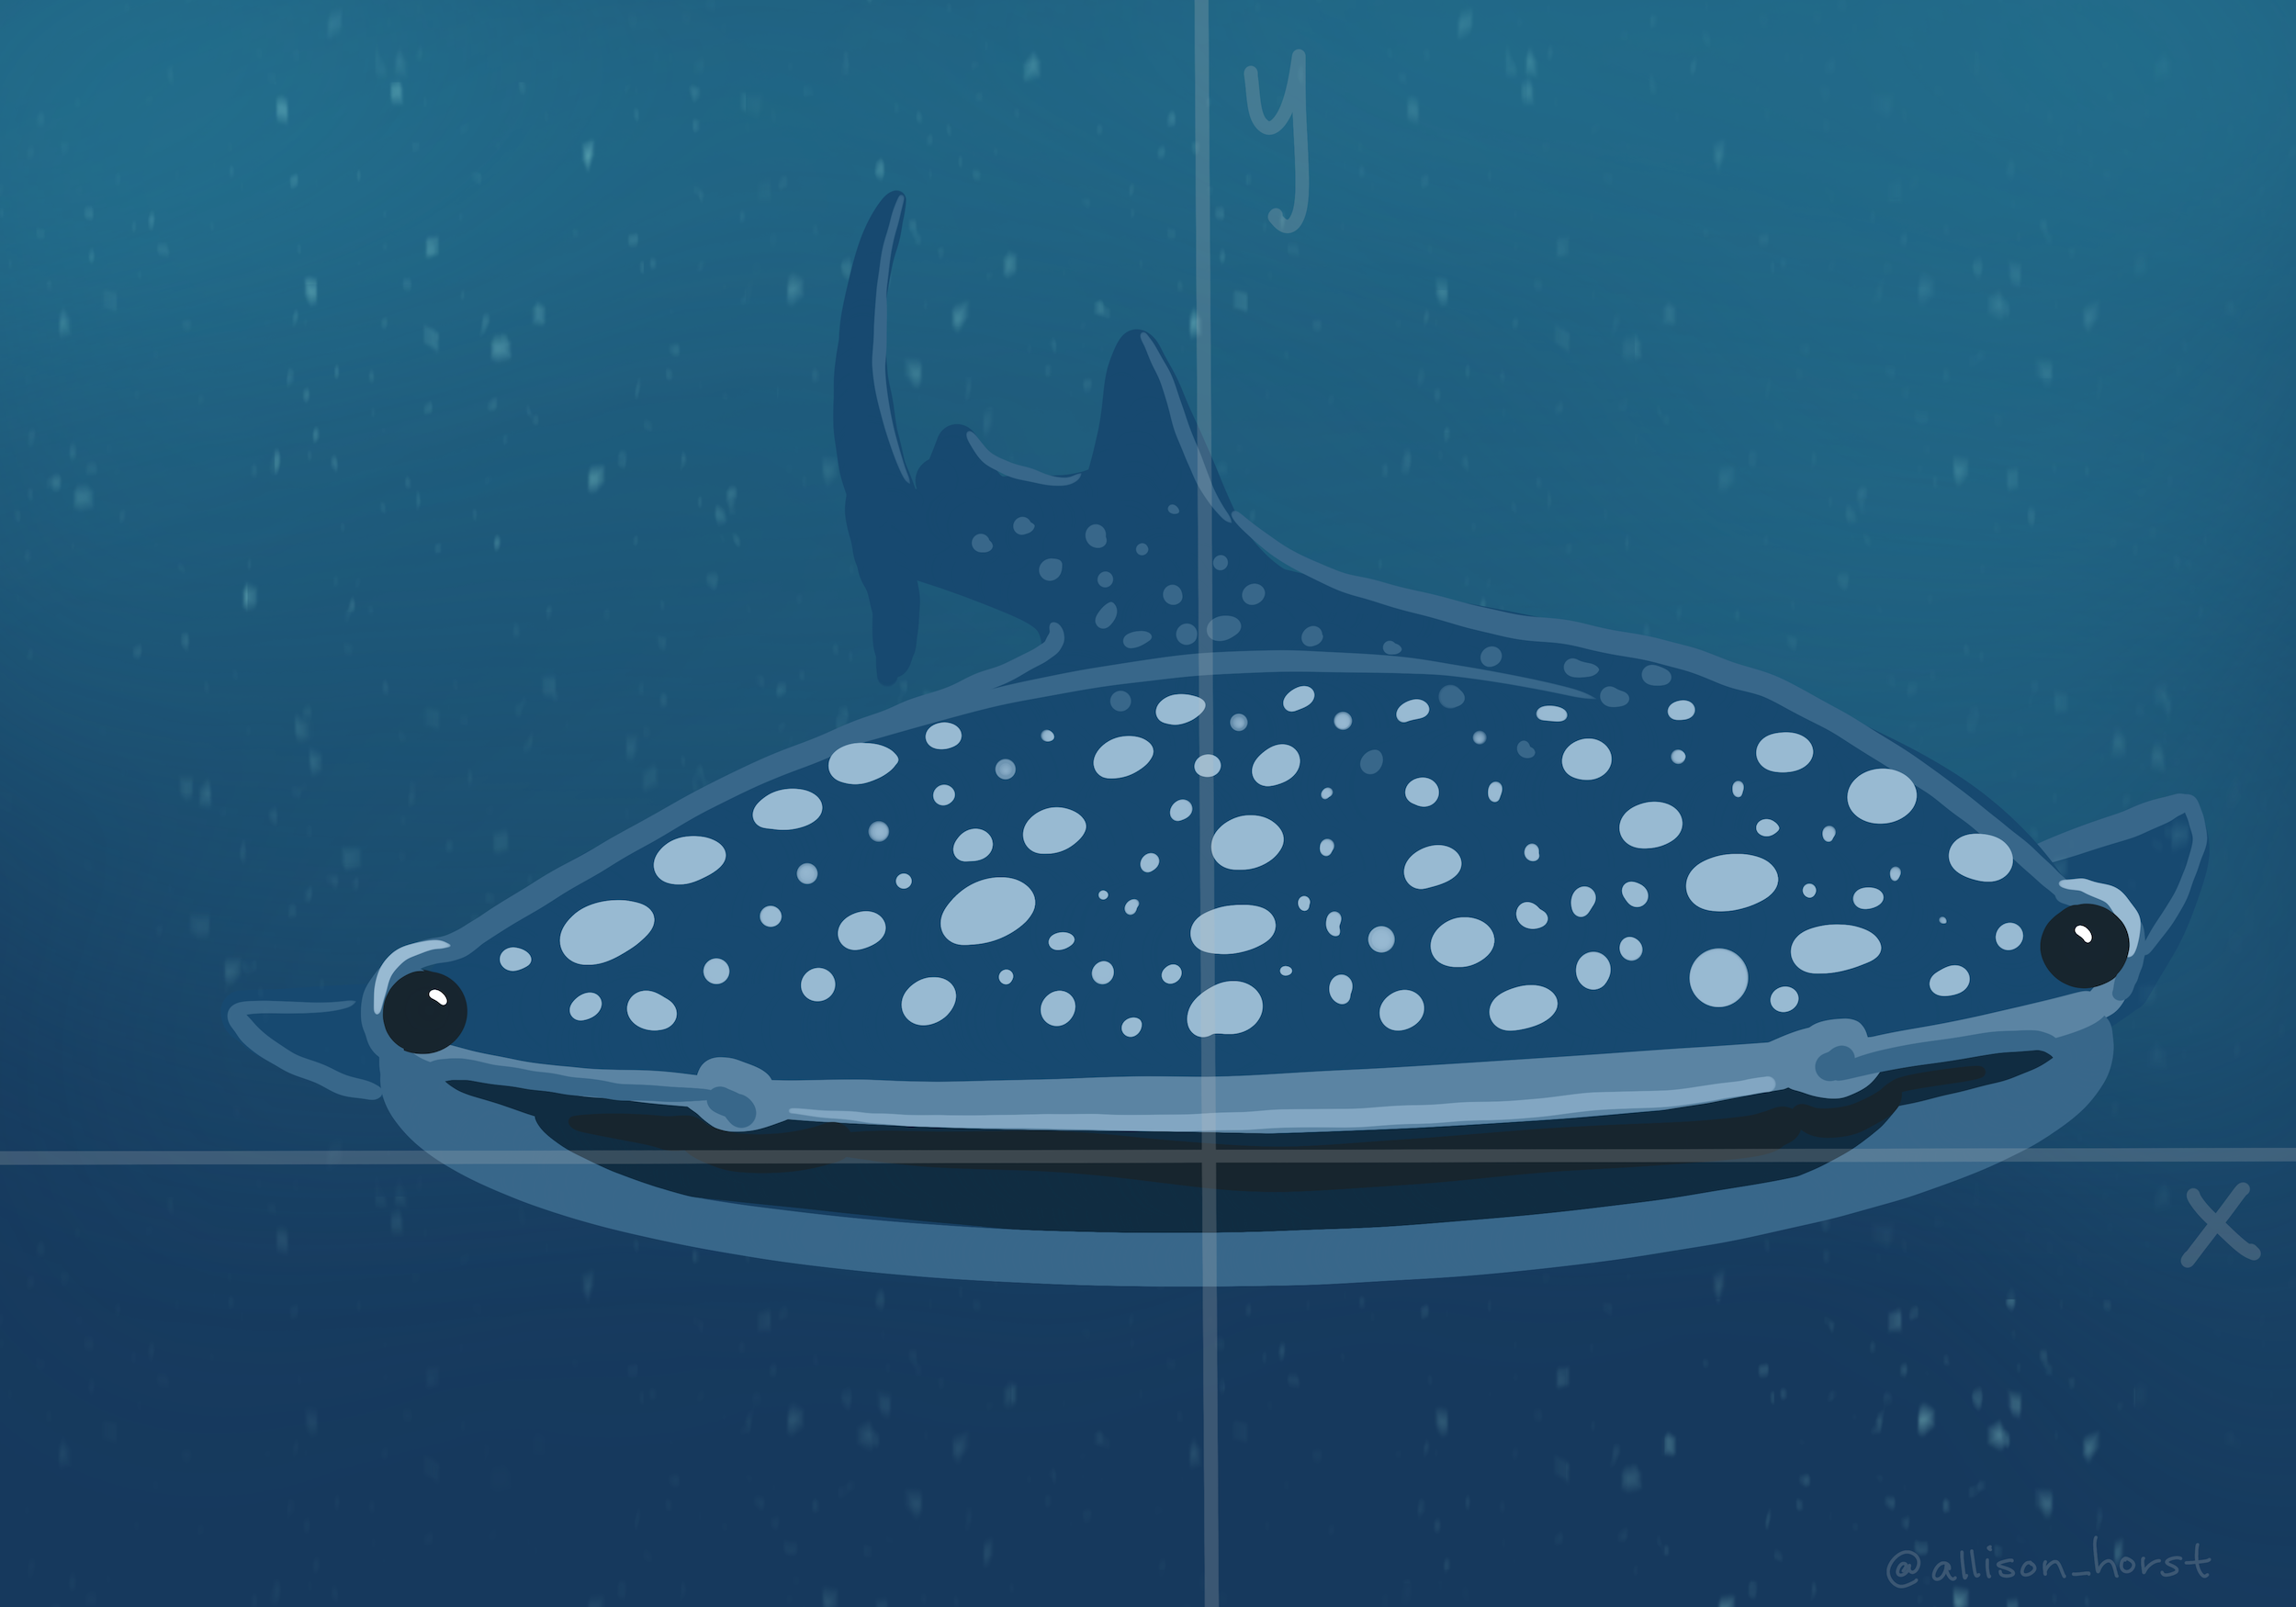
\includegraphics{figs/WideMouthShark1.png}

and that you're swimming towards a delicious swarm of krill.

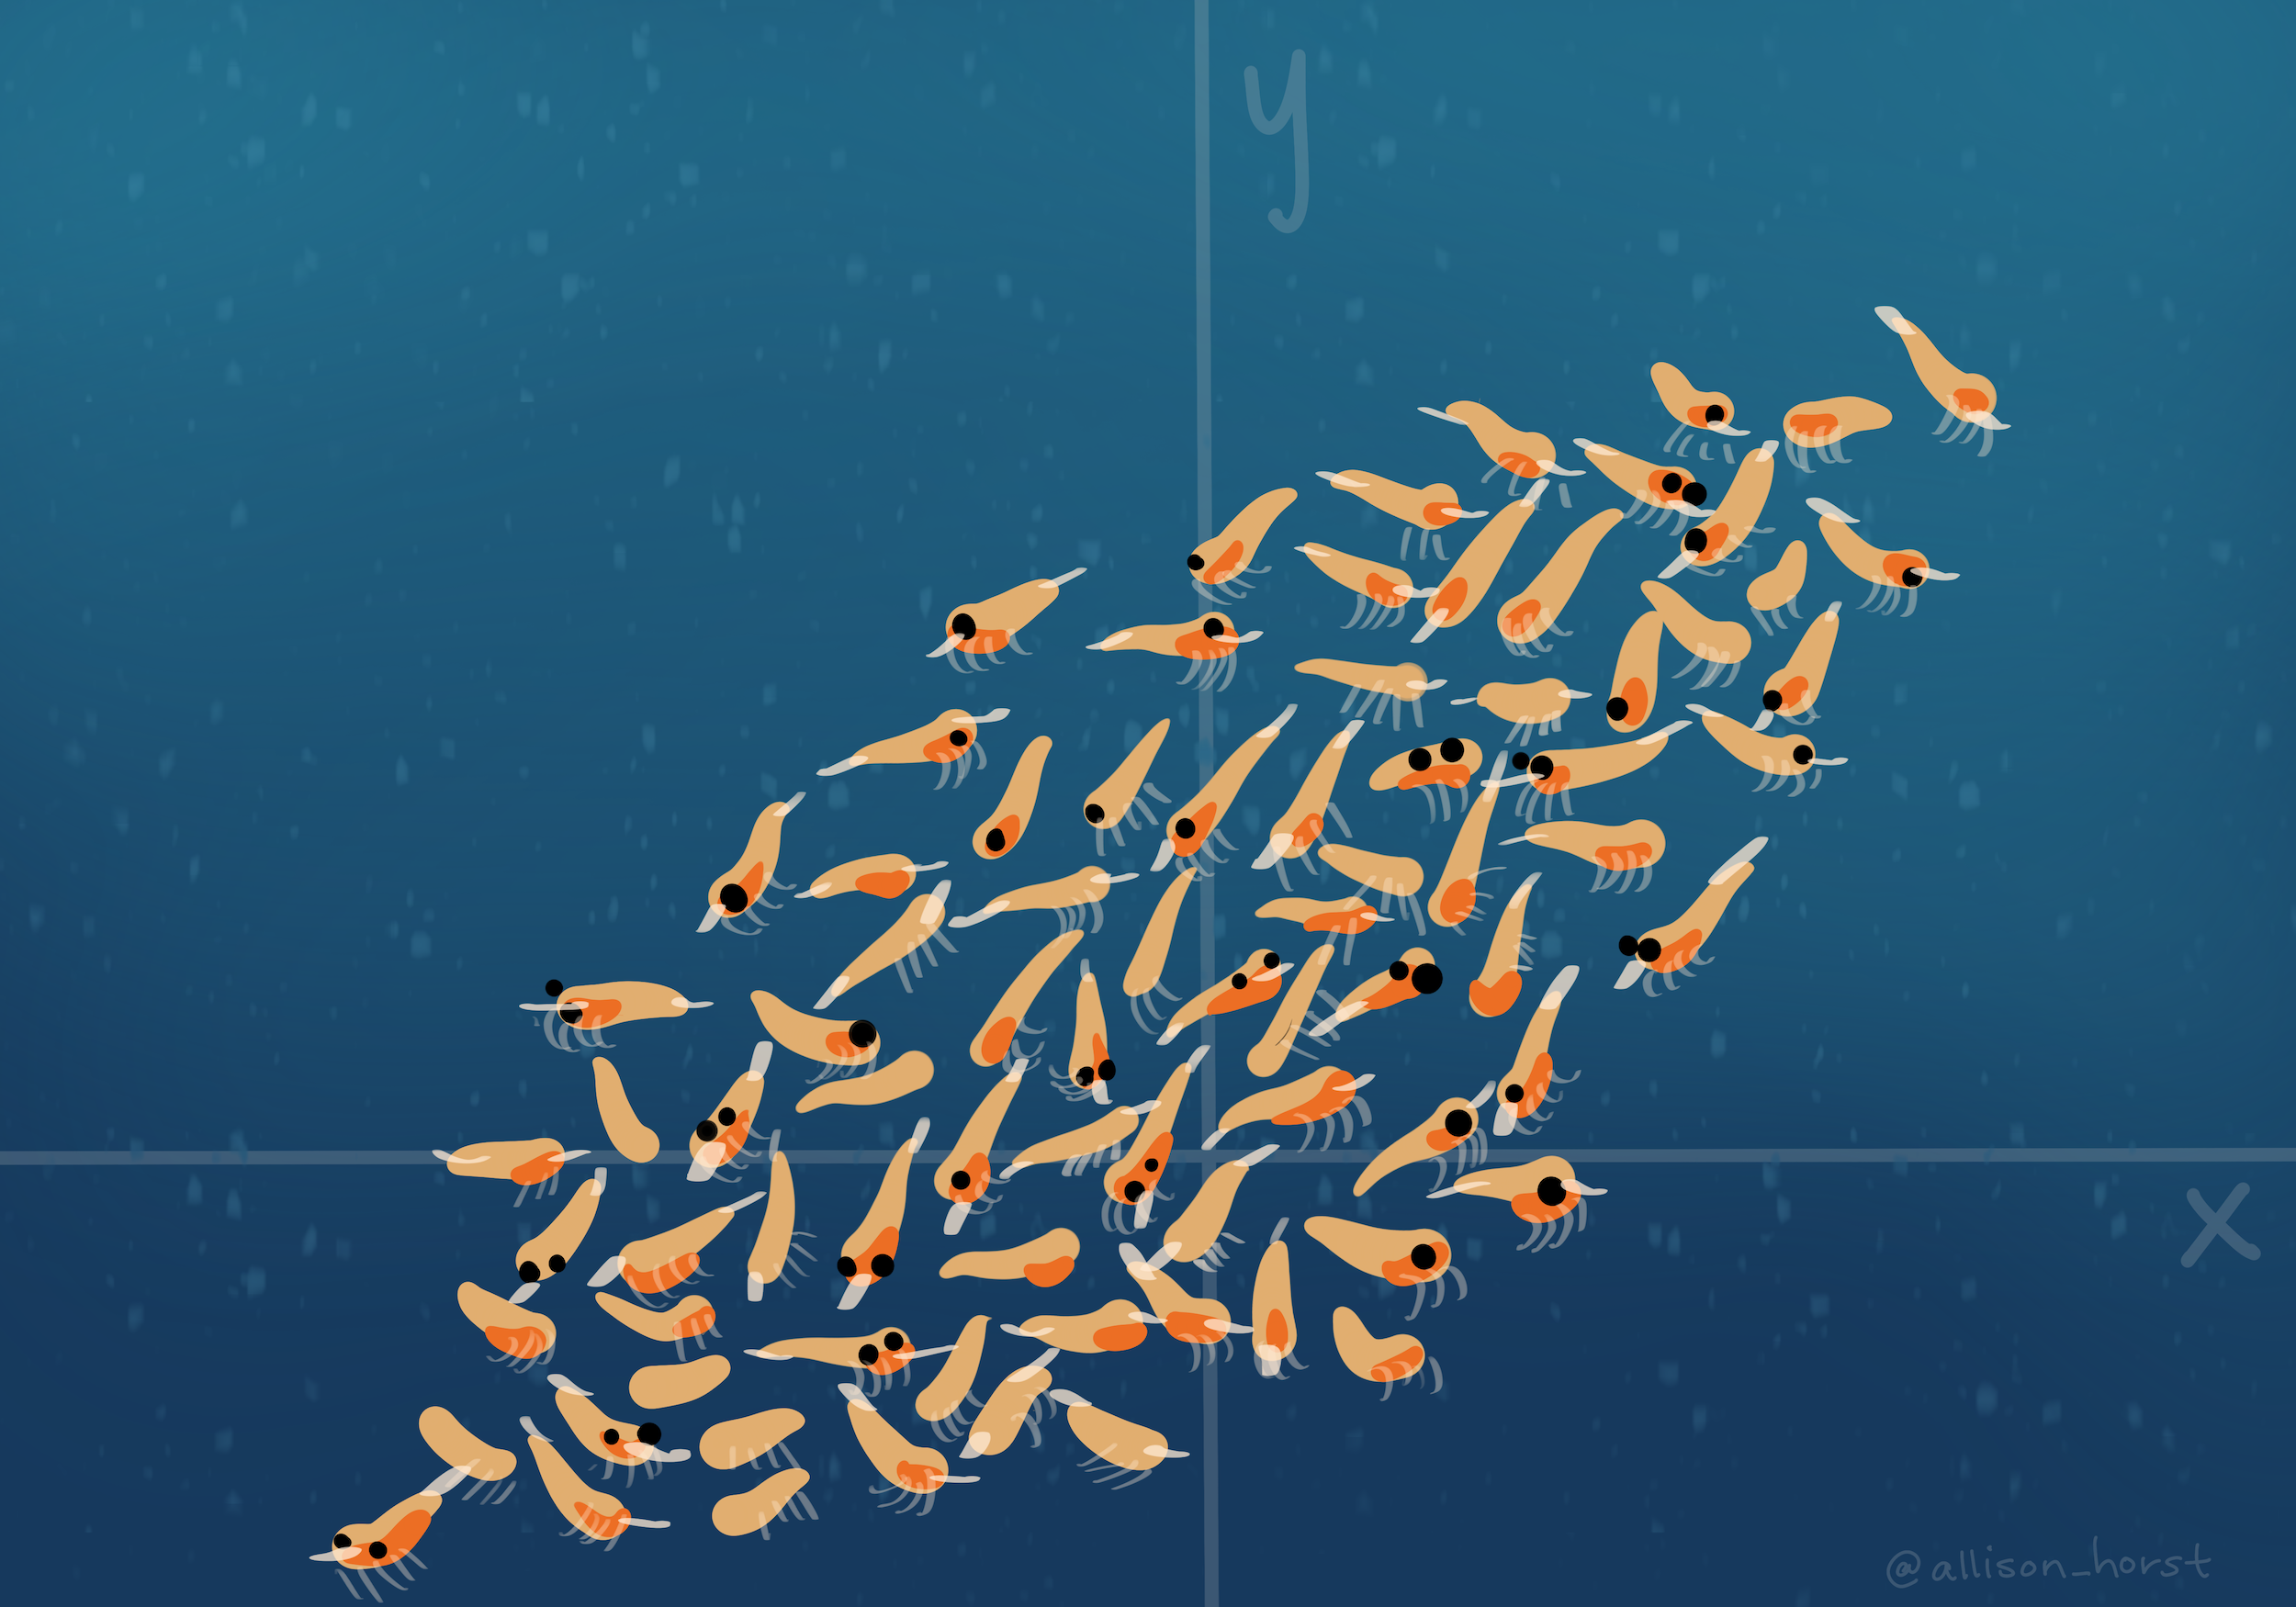
\includegraphics{figs/WideMouthShark2.png}

What way should you tilt your shark head in order to eat as many krill as possible? The answer is given by the first principal component of the data!

\subsection{Notation recap}\label{notation-recap}

As before, let \(\mathbf x_1,\ldots,\mathbf x_n\) be \(p \times 1\) vectors of measurements on \(n\) experimental units and write
\[\mathbf X=\left( \begin{array}{ccc}
- &\mathbf x_1^\top&-\\
- &\mathbf x_2^\top&-\\
- &..&-\\
- &\mathbf x_n^\top&-
\end{array}\right)
\]

\textbf{IMPORTANT NOTE:}
In this section we will assume that \(\mathbf X\) has been column centered so that the mean of each column is \(0\) (i.e., the sample mean of \(\mathbf x_1,\ldots,\mathbf x_n\) is the zero vector \({\boldsymbol 0}\in \mathbb{R}^p\)). If \(\mathbf X\) has not been column centered, replace \(\mathbf X\) by
\[\mathbf H\mathbf X\] where \(\mathbf H\) is the centering matrix (see \ref{centering-matrix}), or equivalently, replace \(\mathbf x_i\) by \(\mathbf x_i - \bar{\mathbf x}\). It is possible to write out the details of PCA replacing \(\mathbf X\) by \(\mathbf H\mathbf X\) throughout, but this gets messy and obscures the important detail. Most software implementations (and in particular \texttt{prcomp} in R), automatically centre your data for you, and so in practice you don't need to worry about doing this when using a software package.

The sample covariance matrix for \(\mathbf X\) (assuming it has been column centered) is
\[\mathbf S= \frac{1}{n}\mathbf X^\top \mathbf X= \frac{1}{n}\sum \mathbf x_i\mathbf x_i^\top\]

Given some vector \(\mathbf u\), the transformed variables
\[y_i = \mathbf u^\top \mathbf x_i\]
have

\begin{itemize}
\item
  \textbf{mean \(0\)}:
  \[\bar{y}= \frac{1}{n}\sum_{i=1}^n y_i = \frac{1}{n}\sum_{i=1}^n \mathbf u^\top \mathbf x_i =\frac{1}{n} \mathbf u^\top \sum_{i=1}^n  \mathbf x_i = 0\]
  as the mean of the \(\mathbf x_i\) is \({\boldsymbol 0}\).
\item
  \textbf{sample covariance matrix} \[\mathbf u^\top \mathbf S\mathbf u\]
  as
  \[\frac{1}{n} \sum_{i=1}^n y_i^2 = \frac{1}{n} \sum_{i=1}^n \mathbf u^\top \mathbf x_i \mathbf x_i^\top\mathbf u= \frac{1}{n}\mathbf u^\top \sum_{i=1}^n  \mathbf x_i \mathbf x_i^\top \mathbf u= \mathbf u^\top \mathbf S\mathbf u
  \]
\end{itemize}

\subsection{First principal component}\label{first-principal-component}

We would like to find the \(\mathbf u\) which maximises the sample variance, \(\mathbf u^\top \mathbf S\mathbf u\) over unit vectors \(\mathbf u\), i.e., vectors with \(||\mathbf u||=1\). Why do we focus on unit vectors? If we don't, we could make the variance as large as we like, e.g., if we replace \(\mathbf u\) by \(10\mathbf u\) it would increase the variance by a factor of 100. Thus, we constrain the problem and only consider unit vectors for \(\mathbf u\).

We know from Proposition \ref{prp:two8} in Section \ref{svdopt} that \(\mathbf v_1\), the first eigenvector of \(\mathbf S\) (also the first right singular vector of \(\mathbf X\)), maximizes \(\mathbf u^\top \mathbf S\mathbf u\) with
\[  \max_{\mathbf u: ||\mathbf u||=1} \mathbf u^\top \mathbf S\mathbf u= \mathbf v_1^\top \mathbf S\mathbf v_1 =\lambda_1\]
where \(\lambda_1\) is the largest eigenvalue of \(\mathbf S\).

So the first principal component of \(\mathbf X\) is \(\mathbf v_1\), and the first transformed variable (sometimes called a principal component score) is \(y_1 = \mathbf v_1 ^\top \mathbf x\).
Applying this to each data point we get \(n\) instances of this new variable
\[y_{i1} = \mathbf v_1 ^\top \mathbf x_i.\]

\textbf{A note on singular values}: We know \(\mathbf S= \frac{1}{n}\mathbf X^\top\mathbf X\) and so the eigenvalues of \(\mathbf S\) are the same as the squared singular values of \(\frac{1}{\sqrt{n}} \mathbf X\):

\[\sqrt{\lambda_1} = \sigma_1\left(\frac{1}{\sqrt{n}} \mathbf X\right)\]

If we scale \(\mathbf X\) by a factor \(c\), then the singular values are scaled by the same amount, i.e.,
\[\sigma_i(c\mathbf X)=c\sigma_i(\mathbf X)\]
and in particular
\[ \sigma_i\left(\frac{1}{\sqrt{n}} \mathbf X\right) = \frac{1}{\sqrt{n}} \sigma_i(\mathbf X)\]
We will need to remember this scaling if we use the SVD of \(\mathbf X\) to do PCA. Note that scaling \(\mathbf X\) does not change the singular vectors/principal components.

\subsection{Second principal component}\label{second-principal-component}

\(y_1\) is the transformed variable that has maximum variance. What should we choose to be our next transformed variable, i.e., what \(\mathbf u_2\) should we choose for \(y_2 = \mathbf u_2^\top \mathbf x\)? It makes sense to choose \(y_2\) to be uncorrelated with \(y_1\), as otherwise it contains some of the same information given by \(y_1\). The sample covariance between \(y_1\) and \(\mathbf u_2^\top \mathbf x\) is
\begin{align*}
s_{y_2y_1} &=\frac{1}{n}\sum_{i=1}^n \mathbf u_2^\top \mathbf x_i \mathbf x_i^\top \mathbf v_1\\ 
&= \mathbf u_2^\top \mathbf S\mathbf v_1\\
& = \lambda_1 \mathbf u_2^\top \mathbf v_1 \mbox{ as } \mathbf v_1 \mbox{ is an eigenvector of } S
\end{align*}
So to make \(y_2\) uncorrelated with \(y_1\) we have to choose \(\mathbf u_2\) to be orthogonal to \(\mathbf v_1\), i.e., \(\mathbf u_2^\top \mathbf v_1=0\). So we choose \(\mathbf u_2\) to be the solution to the optimization problem

\[\max_{\mathbf u} \mathbf u^\top \mathbf S\mathbf u\mbox{ subject to } \mathbf u^\top \mathbf v_1=0.\]
The solution to this problem is to take \(\mathbf u_2 = \mathbf v_2\), i.e., the second eigenvector of \(\mathbf S\) (or second right singular vector of \(\mathbf X\)), and then \[\mathbf v_2^\top \mathbf S\mathbf v_2=\lambda_2.\]
We'll prove this result in the next section.

\subsubsection*{Later principal components}\label{later-principal-components}
\addcontentsline{toc}{subsubsection}{Later principal components}

Our first transformed variable is
\[y_{i1}= \mathbf v_1^\top \mathbf x_i\]
and our second transformed variable is
\[y_{i2}= \mathbf v_2^\top \mathbf x_i.\]
At this point, you can probably guess that the \(j^{th}\) transformed variable is going to be
\[y_{ij}= \mathbf v_j^\top \mathbf x_i.\]
where \(\mathbf v_j\) is the \(j^{th}\) eigenvector of \(\mathbf S\).

\begin{itemize}
\tightlist
\item
  The transformed variables \(y_{i}\) are the \textbf{principal component scores}. \(y_1\) is the first score etc.
\item
  The eigenvectors/right singular vectors are sometimes refered to as the \textbf{loadings} or simply as the \textbf{principal components}.
\end{itemize}

\subsection{Geometric interpretation}\label{geometric-interpretation-1}

We think of PCA as projecting the data points \(\mathbf x\) onto a subspace \(V\). The basis vectors for this subspace are the eigenvectors of \(\mathbf S\), which are the same as the right singular vectors of \(\mathbf X\) (the loadings):
\[V=\operatorname{span}\{\mathbf v_1, \ldots, \mathbf v_r\}.\]
The orthogonal projection matrix (see Section \ref{orthogproj}) for projecting onto \(V\) is
\[\mathbf P_V = \mathbf V\mathbf V^\top\]
as \(\mathbf V^\top \mathbf V=\mathbf I\).\\
The coordinates of the data points projected onto \(V\) (with respect to the basis for \(V\)) are the \textbf{principal component scores}:

\[\mathbf y_i= \left(\begin{array}{c}y_{i1}\\\vdots\\y_{ir}\end{array}\right)= \mathbf V^\top \mathbf x_i\]
where \[\mathbf V= \left(\begin{array}{ccc} | &&|\\\mathbf v_1&\ldots& \mathbf v_r\\  | &&|\end{array}\right)\]
is the matrix of right singular vectors from the SVD of \(\mathbf X\).
The transformed variables are

\[\mathbf Y= \left( \begin{array}{ccc}
- &\mathbf y_1^\top&-\\
- &..&-\\
- &\mathbf y_n^\top&-
\end{array}\right ) = \mathbf X\mathbf V.
\]
Substituting the SVD for \(\mathbf X= \mathbf U\boldsymbol{\Sigma}\mathbf V^\top\) we can see the transformed variable matrix/principal component scores are
\[\mathbf Y= \mathbf U\boldsymbol{\Sigma}.\]

\(\mathbf Y\) is a \(n \times r\) matrix, and so if \(r<p\) we have reduced the dimension of \(\mathbf X\), keeping the most important parts of the data

\subsection{Example}\label{example}

We consider the marks of \(n=10\) students who studied G11PRB and G11STA.

\begin{table}
\centering
\begin{tabular}{rrr}
\toprule
student & PRB & STA\\
\midrule
1 & 81 & 75\\
2 & 79 & 73\\
3 & 66 & 79\\
4 & 53 & 55\\
5 & 43 & 53\\
\addlinespace
6 & 59 & 49\\
7 & 62 & 72\\
8 & 79 & 92\\
9 & 49 & 58\\
10 & 55 & 56\\
\bottomrule
\end{tabular}
\end{table}

These data haven't been column centered, so let's do that in R. You can do it using the centering matrix as previously, but here is a different approach:

\begin{Shaded}
\begin{Highlighting}[]
\NormalTok{secondyr }\OtherTok{\textless{}{-}} \FunctionTok{data.frame}\NormalTok{(}
  \AttributeTok{student =} \DecValTok{1}\SpecialCharTok{:}\DecValTok{10}\NormalTok{,}
\AttributeTok{PRB=}\FunctionTok{c}\NormalTok{(}\DecValTok{81}\NormalTok{ , }\DecValTok{79}\NormalTok{ , }\DecValTok{66}\NormalTok{ , }\DecValTok{53}\NormalTok{ , }\DecValTok{43}\NormalTok{ , }\DecValTok{59}\NormalTok{ , }\DecValTok{62}\NormalTok{ , }\DecValTok{79}\NormalTok{ , }\DecValTok{49}\NormalTok{ , }\DecValTok{55}\NormalTok{),}
\AttributeTok{STA =}\FunctionTok{c}\NormalTok{(}\DecValTok{75}\NormalTok{ , }\DecValTok{73}\NormalTok{ , }\DecValTok{79}\NormalTok{ , }\DecValTok{55}\NormalTok{ , }\DecValTok{53}\NormalTok{ , }\DecValTok{49}\NormalTok{ , }\DecValTok{72}\NormalTok{ , }\DecValTok{92}\NormalTok{ , }\DecValTok{58}\NormalTok{ , }\DecValTok{56}\NormalTok{)}
\NormalTok{        )}
\NormalTok{xbar }\OtherTok{\textless{}{-}} \FunctionTok{colMeans}\NormalTok{(secondyr[,}\DecValTok{2}\SpecialCharTok{:}\DecValTok{3}\NormalTok{]) }\CommentTok{\#only columns 2 and 3 are data}
\NormalTok{X }\OtherTok{\textless{}{-}} \FunctionTok{as.matrix}\NormalTok{(}\FunctionTok{sweep}\NormalTok{(secondyr[,}\DecValTok{2}\SpecialCharTok{:}\DecValTok{3}\NormalTok{], }\DecValTok{2}\NormalTok{, xbar) ) }
\end{Highlighting}
\end{Shaded}

\begin{table}
\centering
\begin{tabular}{rr}
\toprule
PRB & STA\\
\midrule
18.4 & 8.8\\
16.4 & 6.8\\
3.4 & 12.8\\
-9.6 & -11.2\\
-19.6 & -13.2\\
\addlinespace
-3.6 & -17.2\\
-0.6 & 5.8\\
16.4 & 25.8\\
-13.6 & -8.2\\
-7.6 & -10.2\\
\bottomrule
\end{tabular}
\end{table}

The sample covariance matrix can be computed in two ways:

\begin{Shaded}
\begin{Highlighting}[]
\DecValTok{1}\SpecialCharTok{/}\DecValTok{10}\SpecialCharTok{*} \FunctionTok{t}\NormalTok{(X)}\SpecialCharTok{\%*\%}\NormalTok{X}
\end{Highlighting}
\end{Shaded}

\begin{verbatim}
##        PRB    STA
## PRB 162.04 135.38
## STA 135.38 175.36
\end{verbatim}

\begin{Shaded}
\begin{Highlighting}[]
\FunctionTok{cov}\NormalTok{(X)}\SpecialCharTok{*}\DecValTok{9}\SpecialCharTok{/}\DecValTok{10} 
\end{Highlighting}
\end{Shaded}

\begin{verbatim}
##        PRB    STA
## PRB 162.04 135.38
## STA 135.38 175.36
\end{verbatim}

\begin{Shaded}
\begin{Highlighting}[]
\CommentTok{\# Remember R uses the unbiased factor 1/(n{-}1), }
\CommentTok{\# so the 9/10=(n{-}1)/n changes this to 1/n }
\CommentTok{\# to match the notes}
\end{Highlighting}
\end{Shaded}

We can find the singular value decomposition of \(\mathbf X\) using R

\begin{Shaded}
\begin{Highlighting}[]
\NormalTok{(}\AttributeTok{X\_svd =} \FunctionTok{svd}\NormalTok{(X))}
\end{Highlighting}
\end{Shaded}

\begin{verbatim}
## $d
## [1] 55.15829 18.20887
## 
## $u
##              [,1]        [,2]
##  [1,] -0.34556317 -0.39864295
##  [2,] -0.29430029 -0.39482564
##  [3,] -0.21057607  0.34946080
##  [4,]  0.26707104 -0.04226416
##  [5,]  0.41833934  0.27975879
##  [6,]  0.27085156 -0.50812066
##  [7,] -0.06865802  0.24349429
##  [8,] -0.54378479  0.32464825
##  [9,]  0.27768146  0.23043980
## [10,]  0.22893893 -0.08394852
## 
## $v
##            [,1]       [,2]
## [1,] -0.6895160 -0.7242705
## [2,] -0.7242705  0.6895160
\end{verbatim}

So we can see that the eigenvectors/right singular vectors/loadings are

\[\mathbf v_1=\begin{pmatrix} -0.69 \\ -0.724 \end{pmatrix},\qquad \mathbf v_2=\begin{pmatrix} -0.724 \\ 0.69 \end{pmatrix}\]

Sometimes the new variables have an obvious interpretation. In this case the first PC gives approximately equal weight to PRB and STA and thus represents some form of negative `'average'\,' mark. Note that the singular vectors are only determined upto multiplication by \(\pm 1\). In this case, R has chosen \(\mathbf v_1\) to have negative entries, but we could multiply \(\mathbf v_1\) by \(-1\) so that the first PC was more like the avearge.
As it is, a student that has a high mark on PRB and STA will have a low negative value for \(y_1\). The second PC, meanwhile, represents a contrast between PRB and STA. For example, a large positive value for \(y_2\) implies the student did much better on STA than PRB, and a large negative value implies the opposite.

If we plot the data along with the principal components. The two lines, centred on \(\bar{\mathbf x}\), are in the direction of the principal components/eigenvectors, and their lengths are \(2 \sqrt{\lambda_j}\), \(j=1,2\).
We can see that the first PC is in the direction of greatest variation (shown in red), and that the second PC (shown in green) is orthogonal to the first PC.

\includegraphics{04-pca_files/figure-latex/unnamed-chunk-8-1.pdf}

We can find the transformed variables by computing either \(\mathbf X\mathbf V\) or \(\mathbf U\boldsymbol{\Sigma}\)

\begin{Shaded}
\begin{Highlighting}[]
\NormalTok{X }\SpecialCharTok{\%*\%}\NormalTok{ X\_svd}\SpecialCharTok{$}\NormalTok{v}
\end{Highlighting}
\end{Shaded}

\begin{verbatim}
##             [,1]       [,2]
##  [1,] -19.060674 -7.2588361
##  [2,] -16.233101 -7.1893271
##  [3,] -11.615016  6.3632849
##  [4,]  14.731183 -0.7695824
##  [5,]  23.074883  5.0940904
##  [6,]  14.939710 -9.2523011
##  [7,]  -3.787059  4.4337549
##  [8,] -29.994240  5.9114764
##  [9,]  15.316435  4.1960474
## [10,]  12.627880 -1.5286074
\end{verbatim}

\begin{Shaded}
\begin{Highlighting}[]
\NormalTok{X\_svd}\SpecialCharTok{$}\NormalTok{u }\SpecialCharTok{\%*\%} \FunctionTok{diag}\NormalTok{(X\_svd}\SpecialCharTok{$}\NormalTok{d)}
\end{Highlighting}
\end{Shaded}

\begin{verbatim}
##             [,1]       [,2]
##  [1,] -19.060674 -7.2588361
##  [2,] -16.233101 -7.1893271
##  [3,] -11.615016  6.3632849
##  [4,]  14.731183 -0.7695824
##  [5,]  23.074883  5.0940904
##  [6,]  14.939710 -9.2523011
##  [7,]  -3.787059  4.4337549
##  [8,] -29.994240  5.9114764
##  [9,]  15.316435  4.1960474
## [10,]  12.627880 -1.5286074
\end{verbatim}

If we plot the PC scores we can see that the variation is now in line with the new coordinate axes:

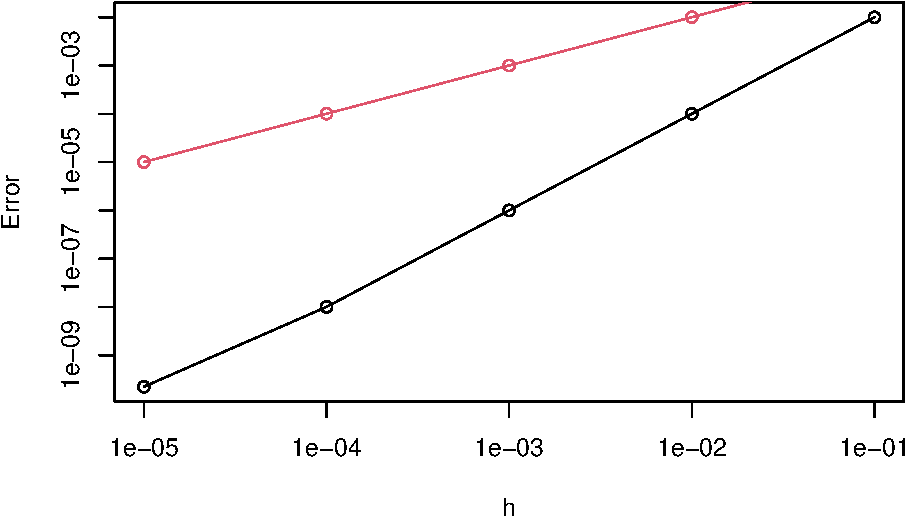
\includegraphics{04-pca_files/figure-latex/unnamed-chunk-10-1.pdf}

R also has a built-in function for doing PCA.

\begin{Shaded}
\begin{Highlighting}[]
\NormalTok{pca }\OtherTok{\textless{}{-}} \FunctionTok{prcomp}\NormalTok{(secondyr[,}\DecValTok{2}\SpecialCharTok{:}\DecValTok{3}\NormalTok{]) }\CommentTok{\# prcomp will automatocally remove the column mean}
\NormalTok{pca}\SpecialCharTok{$}\NormalTok{rotation }\CommentTok{\# the loadings}
\end{Highlighting}
\end{Shaded}

\begin{verbatim}
##            PC1        PC2
## PRB -0.6895160 -0.7242705
## STA -0.7242705  0.6895160
\end{verbatim}

\begin{Shaded}
\begin{Highlighting}[]
\NormalTok{pca}\SpecialCharTok{$}\NormalTok{x }\CommentTok{\# the scores}
\end{Highlighting}
\end{Shaded}

\begin{verbatim}
##              PC1        PC2
##  [1,] -19.060674 -7.2588361
##  [2,] -16.233101 -7.1893271
##  [3,] -11.615016  6.3632849
##  [4,]  14.731183 -0.7695824
##  [5,]  23.074883  5.0940904
##  [6,]  14.939710 -9.2523011
##  [7,]  -3.787059  4.4337549
##  [8,] -29.994240  5.9114764
##  [9,]  15.316435  4.1960474
## [10,]  12.627880 -1.5286074
\end{verbatim}

Note that the new variables have sample mean \(\bar{\mathbf y}={\boldsymbol 0}\). The sample covariance matrix is a diagonal with entries given by the eigenvalues (see part 4. of Proposition \ref{prp:pca2}). Note that there is always some numerical error (so quantities are never 0, and instead are just very small numbers).

\[
\boldsymbol \Lambda= \text{diag}(\lambda_1,\lambda_2) =  \begin{pmatrix} \lambda_1 & 0 \\ 0 & \lambda_2 \end{pmatrix}.
\]

\begin{Shaded}
\begin{Highlighting}[]
\FunctionTok{colMeans}\NormalTok{(pca}\SpecialCharTok{$}\NormalTok{x)}
\end{Highlighting}
\end{Shaded}

\begin{verbatim}
##           PC1           PC2 
##  2.797762e-15 -7.993606e-16
\end{verbatim}

\begin{Shaded}
\begin{Highlighting}[]
\FunctionTok{cov}\NormalTok{(pca}\SpecialCharTok{$}\NormalTok{x)}\SpecialCharTok{*}\DecValTok{9}\SpecialCharTok{/}\DecValTok{10} \CommentTok{\# to convert to using 1/n as the denominator }
\end{Highlighting}
\end{Shaded}

\begin{verbatim}
##               PC1           PC2
## PC1  3.042437e+02 -7.498429e-14
## PC2 -7.498429e-14  3.315628e+01
\end{verbatim}

Finally, note that we did the singular value decomposition for \(\mathbf X\) above not \(\frac{1}{\sqrt{10}}\mathbf X\), and so we'd need to square and scale the singular values to find the eigenvalues. Let's check:

\begin{Shaded}
\begin{Highlighting}[]
\NormalTok{X\_svd}\SpecialCharTok{$}\NormalTok{d}\SpecialCharTok{\^{}}\DecValTok{2}\SpecialCharTok{/}\DecValTok{10} \CommentTok{\# square and scale the singular values}
\end{Highlighting}
\end{Shaded}

\begin{verbatim}
## [1] 304.24372  33.15628
\end{verbatim}

\begin{Shaded}
\begin{Highlighting}[]
\FunctionTok{eigen}\NormalTok{(}\FunctionTok{t}\NormalTok{(X) }\SpecialCharTok{\%*\%}\NormalTok{ X}\SpecialCharTok{/}\DecValTok{10}\NormalTok{)}\SpecialCharTok{$}\NormalTok{values  }
\end{Highlighting}
\end{Shaded}

\begin{verbatim}
## [1] 304.24372  33.15628
\end{verbatim}

\begin{Shaded}
\begin{Highlighting}[]
\CommentTok{\# compute the eigenvalues of the covariance matrix}
\FunctionTok{svd}\NormalTok{(X}\SpecialCharTok{/}\FunctionTok{sqrt}\NormalTok{(}\DecValTok{10}\NormalTok{))}\SpecialCharTok{$}\NormalTok{d}\SpecialCharTok{\^{}}\DecValTok{2} 
\end{Highlighting}
\end{Shaded}

\begin{verbatim}
## [1] 304.24372  33.15628
\end{verbatim}

\begin{Shaded}
\begin{Highlighting}[]
\CommentTok{\# compute the singular values of X/sqrt(10) and square}
\end{Highlighting}
\end{Shaded}

\subsection{Example: Iris}\label{example-iris}

In general when using R to do PCA, we don't need to compute the SVD and then do the projections, as there is an R command \texttt{prcomp} that will do it all for us. The \texttt{princomp} will also do PCA, but is less stable than \texttt{prcomp}, and it is recommended that you use \texttt{prcomp} in preference.

Let's do PCA on the iris dataset discussed in Chapter \ref{stat-prelim}. The \texttt{prcomp} returns the square root of the eigenvalues (the standard devaiation of the PC scores), and the PC scores.

\begin{Shaded}
\begin{Highlighting}[]
\NormalTok{iris.pca }\OtherTok{=} \FunctionTok{prcomp}\NormalTok{(iris[,}\DecValTok{1}\SpecialCharTok{:}\DecValTok{4}\NormalTok{])}
\NormalTok{iris.pca}\SpecialCharTok{$}\NormalTok{sdev }\CommentTok{\# the square root of the eigenvalues}
\end{Highlighting}
\end{Shaded}

\begin{verbatim}
## [1] 2.0562689 0.4926162 0.2796596 0.1543862
\end{verbatim}

\begin{Shaded}
\begin{Highlighting}[]
\FunctionTok{head}\NormalTok{(iris.pca}\SpecialCharTok{$}\NormalTok{x)  }\CommentTok{\#the PC scores}
\end{Highlighting}
\end{Shaded}

\begin{verbatim}
##            PC1        PC2         PC3          PC4
## [1,] -2.684126 -0.3193972  0.02791483  0.002262437
## [2,] -2.714142  0.1770012  0.21046427  0.099026550
## [3,] -2.888991  0.1449494 -0.01790026  0.019968390
## [4,] -2.745343  0.3182990 -0.03155937 -0.075575817
## [5,] -2.728717 -0.3267545 -0.09007924 -0.061258593
## [6,] -2.280860 -0.7413304 -0.16867766 -0.024200858
\end{verbatim}

The PC loadings/eigenvectors can also be accessed, as can the sample mean

\begin{Shaded}
\begin{Highlighting}[]
\NormalTok{iris.pca}\SpecialCharTok{$}\NormalTok{rotation }\CommentTok{\#the eigenvecstors}
\end{Highlighting}
\end{Shaded}

\begin{verbatim}
##                      PC1         PC2         PC3        PC4
## Sepal.Length  0.36138659 -0.65658877  0.58202985  0.3154872
## Sepal.Width  -0.08452251 -0.73016143 -0.59791083 -0.3197231
## Petal.Length  0.85667061  0.17337266 -0.07623608 -0.4798390
## Petal.Width   0.35828920  0.07548102 -0.54583143  0.7536574
\end{verbatim}

\begin{Shaded}
\begin{Highlighting}[]
\NormalTok{iris.pca}\SpecialCharTok{$}\NormalTok{center }\CommentTok{\# the sample mean of the data}
\end{Highlighting}
\end{Shaded}

\begin{verbatim}
## Sepal.Length  Sepal.Width Petal.Length  Petal.Width 
##     5.843333     3.057333     3.758000     1.199333
\end{verbatim}

A scree plot can be obtained simply by using the \texttt{plot} command. The summary command also gives useful information about the importance of each PC.

\begin{Shaded}
\begin{Highlighting}[]
\FunctionTok{plot}\NormalTok{(iris.pca)}
\end{Highlighting}
\end{Shaded}

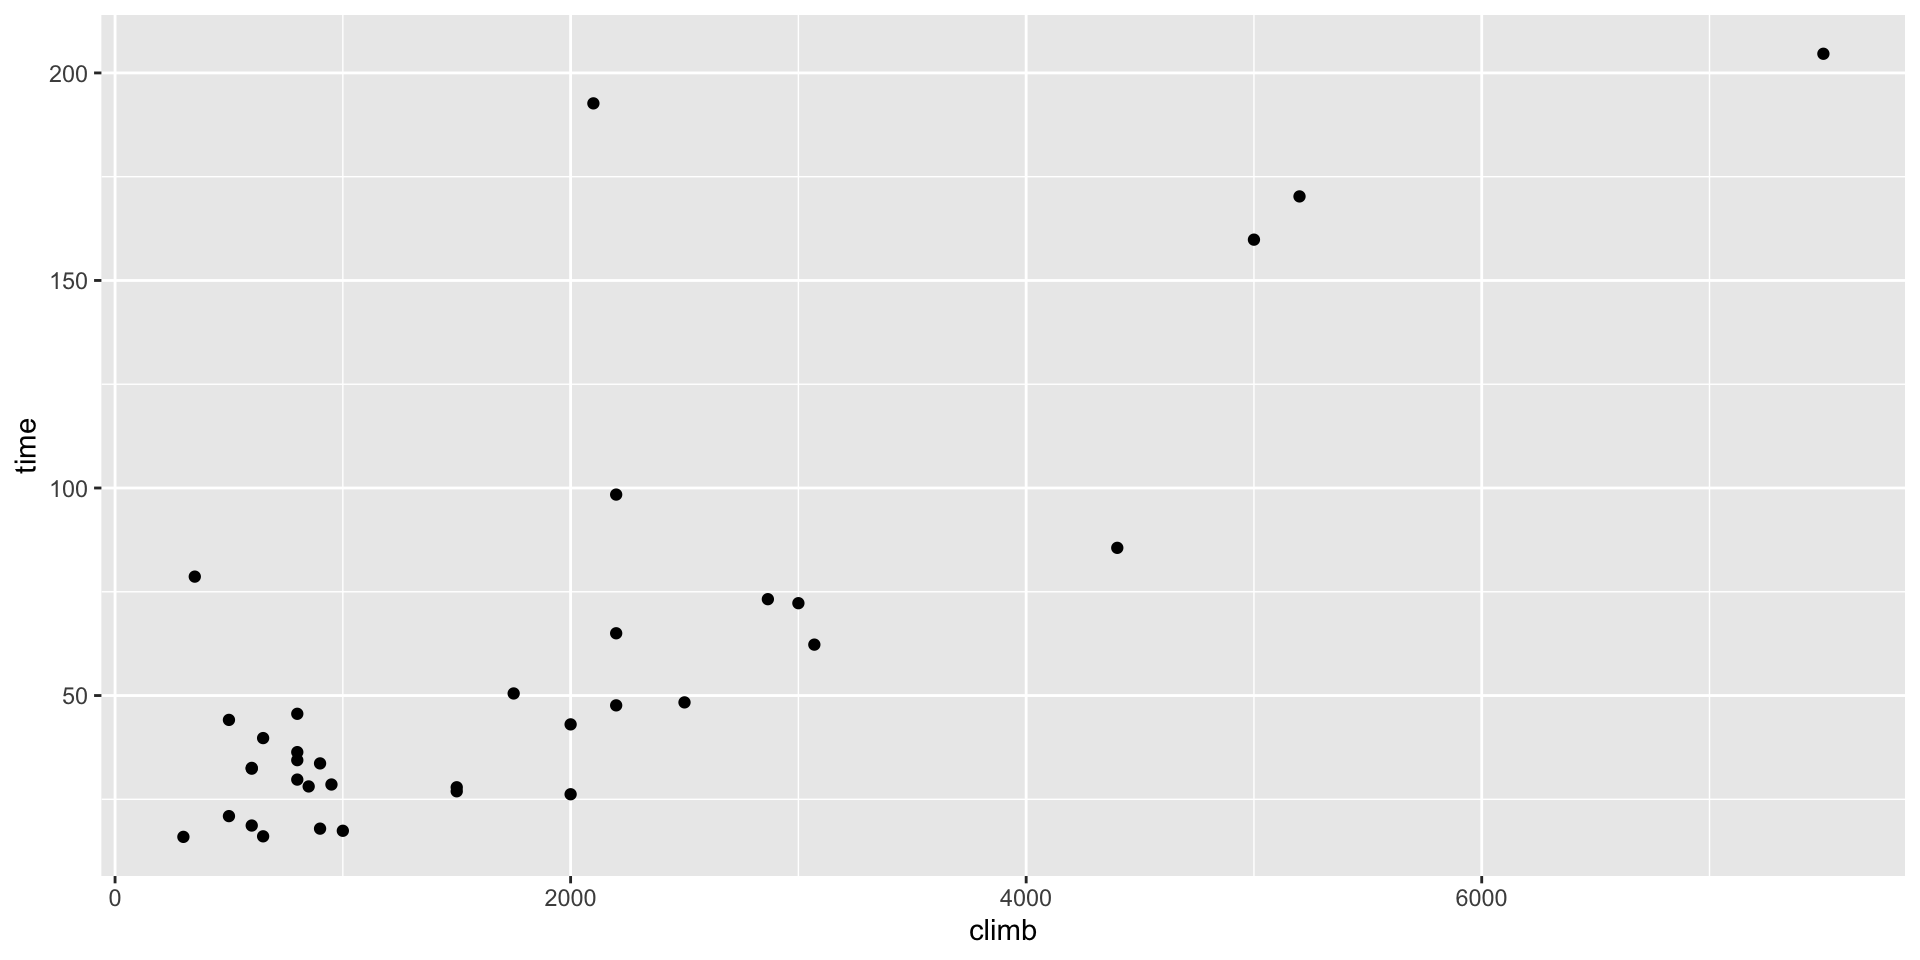
\includegraphics{04-pca_files/figure-latex/unnamed-chunk-16-1.pdf}

\begin{Shaded}
\begin{Highlighting}[]
\FunctionTok{summary}\NormalTok{(iris.pca)}
\end{Highlighting}
\end{Shaded}

\begin{verbatim}
## Importance of components:
##                           PC1     PC2    PC3     PC4
## Standard deviation     2.0563 0.49262 0.2797 0.15439
## Proportion of Variance 0.9246 0.05307 0.0171 0.00521
## Cumulative Proportion  0.9246 0.97769 0.9948 1.00000
\end{verbatim}

To plot the PC scores, you can either manually create a plot or use the \texttt{ggfortify} package. For example, here is a plot of the first two PC scores coloured according to the species of iris.

\begin{Shaded}
\begin{Highlighting}[]
\NormalTok{iris}\SpecialCharTok{$}\NormalTok{PC1}\OtherTok{=}\NormalTok{iris.pca}\SpecialCharTok{$}\NormalTok{x[,}\DecValTok{1}\NormalTok{]}
\NormalTok{iris}\SpecialCharTok{$}\NormalTok{PC2}\OtherTok{=}\NormalTok{iris.pca}\SpecialCharTok{$}\NormalTok{x[,}\DecValTok{2}\NormalTok{]}
\NormalTok{iris }\SpecialCharTok{|\textgreater{}} \FunctionTok{ggplot}\NormalTok{(}\FunctionTok{aes}\NormalTok{(}\AttributeTok{x=}\NormalTok{PC1, }\AttributeTok{y=}\NormalTok{PC2, }\AttributeTok{colour=}\NormalTok{Species))}\SpecialCharTok{+}\FunctionTok{geom\_point}\NormalTok{()}
\end{Highlighting}
\end{Shaded}

\includegraphics{04-pca_files/figure-latex/unnamed-chunk-17-1.pdf}

The \texttt{ggfortify} package provides a nice wrapper for some of this functionality.

\begin{Shaded}
\begin{Highlighting}[]
\FunctionTok{library}\NormalTok{(ggfortify)}
\FunctionTok{autoplot}\NormalTok{(iris.pca, }\AttributeTok{data =}\NormalTok{ iris, }\AttributeTok{colour =} \StringTok{\textquotesingle{}Species\textquotesingle{}}\NormalTok{, }\AttributeTok{scale=}\ConstantTok{FALSE}\NormalTok{)}
\end{Highlighting}
\end{Shaded}

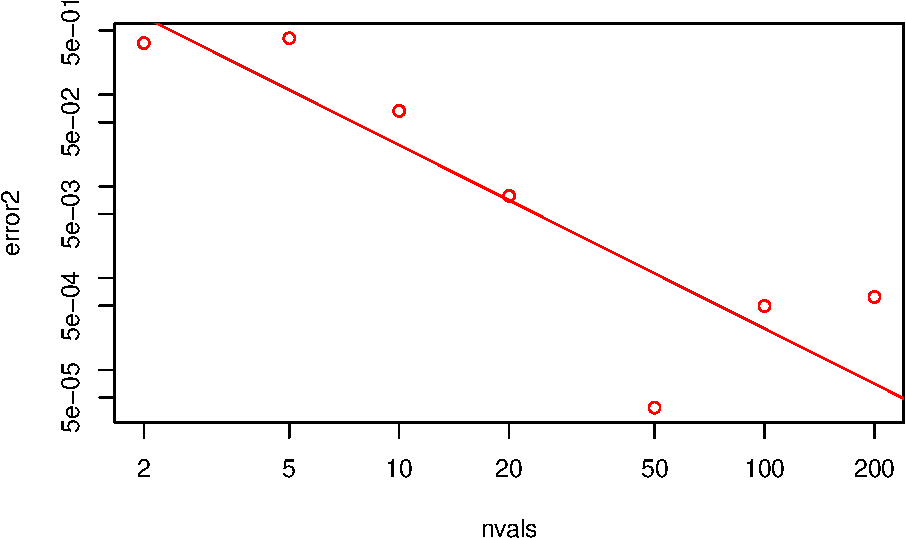
\includegraphics{04-pca_files/figure-latex/unnamed-chunk-18-1.pdf}

\section{PCA: a formal description with proofs}\label{pca-a-formal-description-with-proofs}

Let's now summarize what we've said so far and prove some results about principal component analysis.

Let \(\mathbf x_1, \ldots , \mathbf x_n\) denote a sample of vectors in \(\mathbb{R}^p\) with sample mean vector \(\bar{\mathbf x}\) and sample covariance matrix \(\mathbf S\). Suppose \(\mathbf S=\frac{1}{n}\mathbf X^\top \mathbf H\mathbf X\) has spectral decomposition (see Proposition \ref{prp:spectraldecomp})
\begin{equation}
\mathbf S=\mathbf V\boldsymbol \Lambda\mathbf V^\top = \sum_{j=1}^p  \lambda_j \mathbf v_j \mathbf v_j^\top,
\label{eq:pcaspect}
\end{equation}
where the eigenvalues are \(\lambda_1 \geq \lambda_2 \geq \lambda_p \geq 0\) with \(\boldsymbol \Lambda=\text{diag}\{\lambda_1, \ldots, \lambda_p\}\), and \(\mathbf V\) contains the eigenvectors of \(\mathbf S\). If \(\mathbf S\) is of full rank, then \(\lambda_p>0\). If \(\mathbf S\) is rank \(r\), with \(r<p\), then \(\lambda_{r+1}=\ldots \lambda_p=0\) and we can truncate \(\mathbf V\) to consider just the first \(r\) columns.

The principal components of \(\mathbf X\) are defined sequentially. If the \(\mathbf v_k\) is value of \(\mathbf u\) that maximizes the objective for the \(k^{th}\) problem (for \(k<j\)), then the \(j^{th}\) principal component is the solution to the following optimization problem:
\begin{equation}
\max_{\mathbf u: \, \vert \vert \mathbf u\vert \vert =1}\mathbf u^\top \mathbf S\mathbf u
\label{eq:pcmaxgen}
\end{equation}
subject to
\begin{equation}
\mathbf v_k^\top \mathbf u=0, \qquad k=1, \ldots , j-1.
\label{eq:pccongen}
\end{equation}
(for \(j=1\) there is no orthogonality constraint).

\begin{proposition}
\protect\hypertarget{prp:pca1}{}\label{prp:pca1}The maximum of Equation \eqref{eq:pcmaxgen}
subject to Equation \eqref{eq:pccongen} is equal to \(\lambda_j\) and is obtained when \(\mathbf u=\mathbf v_j\).
\end{proposition}

\begin{proof}
We can prove this using the method of Lagrange multipliers. For \(j=1\) our objective is
\[\mathcal{L} = \mathbf u^\top  \mathbf S\mathbf u+\lambda(1-\mathbf u^\top \mathbf u)\]
Differentiating (see \ref{vectordiff}) with respect to \(\mathbf u\) and setting the derivative equal to zero gives
\[2\mathbf S\mathbf u-2\lambda \mathbf u=0\]
Rearranging we see that \(\mathbf u\) must satify
\[\mathbf S\mathbf u=\lambda \mathbf u\mbox{ with } \mathbf u^\top \mathbf u=1\]
i.e., \(\mathbf u\) is a unit eigenvector of \(\mathbf S\). Substituting this back in to the objective we see
\[\mathbf u^\top \mathbf S\mathbf u= \lambda\]
and so we must choose \(\mathbf u=\mathbf v_1\), the eigenvector corresponding to the largest eigenvalue of \(\mathbf S\).

We now proceed inductively and assume the result is true for \(k=1, \ldots, j-1\). The Lagrangian for the \(j^{th}\) optimization problem is
\[\mathcal{L} = \mathbf u^\top  \mathbf S\mathbf u+\lambda(1-\mathbf u^\top \mathbf u) +\sum_{k=1}^{j-1}\mu_k (0-\mathbf u^\top \mathbf v_k)\]
where we now have \(j\) Lagrange multipliers \(\lambda, \mu_1, \ldots, \mu_{j-1}\) - one for each constraint.
Differentiating with respect to \(\mathbf u\) and setting equal to zero gives
\[2\mathbf S\mathbf u- 2\lambda \mathbf u- \sum_{k=1}^{j-1} \mu_k\mathbf v_k=0 \]
If we left multiply by \(\mathbf v_l^\top\) we get
\[2\mathbf v_l^\top \mathbf S\mathbf u- 2\lambda \mathbf v_l^\top \mathbf u- \sum \mu_k \mathbf v_l^\top \mathbf v_k =0\]
We know \(\mathbf v_l\) is an eigenvector of \(\mathbf S\) and so \(\mathbf S\mathbf v_l=\lambda_l \mathbf v_l\) and hence \(\mathbf v_l^\top \mathbf S\mathbf u=0\) as \(\mathbf v_l^\top \mathbf u=0\). Also \[\mathbf v_l^\top\mathbf v_k=\begin{cases}1 &\mbox{ if } k=l\\
0 &\mbox{ otherwise, }\end{cases}\] and thus we've shown that \(\mu_l=0\) for \(l=1, \ldots, j-1\). So again we have that \[\mathbf S\mathbf u= \lambda \mathbf u\]
i.e., \(\mathbf u\) must be a unit eigenvector of \(\mathbf S\). It only remains to show \emph{which} eigenvector it is. Because \(\mathbf u\) must be orthogonal to \(\mathbf v_1, \ldots, \mathbf v_{j-1}\),
and as \(\mathbf v_l^\top \mathbf S\mathbf v_l = \lambda_l\), we must choose \(\mathbf u=\mathbf v_j\), the eigenvector corresponding to the \(j^{th}\) largest eigenvalue.
\end{proof}

\subsection{Properties of principal components}\label{properties-of-principal-components}

For \(j=1, \ldots , p\), the scores of the \(j^{th}\) principal component (PC) are given by
\[
y_{ij}=\mathbf v_j^\top(\mathbf x_i - \bar{\mathbf x}), \qquad i=1, \ldots , n.
\]
The \(j^{th}\) eigenvector \(\mathbf v_j\) is sometimes referred to as the vector of \textbf{loadings} for the \(j^{th}\) PC. Note that if \(\operatorname{rank}(\mathbf S)=r<p\), then the \(r+1^{th}, \ldots, p^{th}\) scores are meaningless, as they will all be zero.

In vector notation
\[
\mathbf y_i=( y_{i1}, y_{i2}, \ldots , y_{ip})^\top = \mathbf V^\top (\mathbf x_i -\bar{\mathbf x}), \qquad i=1, \ldots ,n.
\]
In matrix form, the full set of PC scores is given by
\[
\mathbf Y= [\mathbf y_1 , \ldots , \mathbf y_n]^\top =\mathbf H\mathbf X\mathbf V.
\]

If \(\tilde{\mathbf X}=\mathbf H\mathbf X\) is the column centered data matrix, with singular value decomposition
\(\tilde{\mathbf X}=\mathbf U\boldsymbol{\Sigma}\mathbf V^\top\) with \(\mathbf V\) as in Equation \eqref{eq:pcaspect}, then
\[\mathbf Y= \tilde{\mathbf X}\mathbf V= \mathbf U\boldsymbol{\Sigma}.\]

The transformed variables \(\mathbf Y= \mathbf H\mathbf X\mathbf V\) have some important properties which we collect together in the following proposition.

\begin{proposition}
\protect\hypertarget{prp:pca2}{}\label{prp:pca2}

The following results hold:

\begin{enumerate}
\def\labelenumi{\arabic{enumi}.}
\item
  The sample mean vector of \(\mathbf y_1, \ldots , \mathbf y_n\) is the zero vector: \(\bar{\mathbf y}={\mathbf 0}_p\)
\item
  The sample covariance matrix of \(\mathbf y_1, \ldots, \mathbf y_n\) is
  \[\Lambda = \operatorname{diag}(\lambda_1, \ldots, \lambda_p)\]
  i.e., for each fixed \(j\), the sample variance of \(y_{ij}\) is \(\lambda_j\), and \(y_{ij}\) is uncorrelated with \(y_{ik}\) for \(j\not = k\).
\item
  For \(j\leq k\) the sample variance of \(\{y_{ij}\}_{i=1, \ldots , n}\) is greater than or equal to the sample variance of \(\{y_{ik}\}_{i=1, \ldots , n}\).
  \[\mathbf v_1^\top \mathbf S\mathbf v_1 \geq \mathbf v_2^\top \mathbf S\mathbf v_2 \geq \ldots \geq \mathbf v_p^\top \mathbf S\mathbf v_p\geq 0\]
  Note that if \(\operatorname{rank}(\mathbf S)=r<p\), then \(\mathbf v_k^\top \mathbf S\mathbf v_k = 0\) for \(k=r+1, \ldots, p\).
\item
  The sum of the sample variances is equal to the trace of \(\mathbf S\)
  \[\sum_{j=1}^p \mathbf v_j^\top \mathbf S\mathbf v_j = \sum_{j=1}^p \lambda_j = \text{tr}(\mathbf S)\]
\item
  The product of the sample variances is equal to the determinant of \(\mathbf S\)
  \[\prod_{j=1}^p \mathbf v_j^\top \mathbf S\mathbf v_j = \prod_{j=1}^p \lambda_j = |\mathbf S|.\]
\end{enumerate}

\end{proposition}

\begin{proof}

For i.
\[\bar{\mathbf y} = \frac{1}{n}\sum_{i=1}^n \mathbf V^\top(\mathbf x_i-\bar{\mathbf x}) = \frac{1}{n} \mathbf V^\top\sum_{i=1}^n(\mathbf x_i-\bar{\mathbf x}) ={\boldsymbol 0}.\]

For 2. the sample covariance matrix of \(\mathbf y_1, \ldots, \mathbf y_n\) is
\begin{align*}
\frac{1}{n}\sum_{i=1}^n \mathbf y_i \mathbf y_i^\top &=\frac{1}{n} \sum \mathbf V^\top (\mathbf x_i-\bar{\mathbf x})(\mathbf x_i - \mathbf x)^\top \mathbf V\\
&=\mathbf V^\top \mathbf S\mathbf V\\
&=\mathbf V^\top \mathbf V\boldsymbol \Lambda\mathbf V^\top \mathbf V\mbox{ substiting the spectral decomposition for }\mathbf S\\
&=\boldsymbol \Lambda
\end{align*}

\begin{enumerate}
\def\labelenumi{\arabic{enumi}.}
\setcounter{enumi}{2}
\item
  is a consequence 2. and of ordering the eigenvalues in decreasing magnitude.
\item
  follows from lemma \ref{lem:trace} and the spectral decomposition of \(\mathbf S\):
  \[\operatorname{tr}(\mathbf S) = \operatorname{tr}(\mathbf V\boldsymbol \Lambda\mathbf V^\top)  =\operatorname{tr}(\mathbf V^\top \mathbf V\boldsymbol \Lambda)=\operatorname{tr}(\boldsymbol \Lambda)=\sum\lambda_i\]
\item
  follows from \ref{prp:deteig}.
\end{enumerate}

\end{proof}

From these properties we say that a proportion
\[\frac{\lambda_j}{\lambda_1 + \ldots + \lambda_p}\]
of the variability in the sample is `explained' by the \(j^{th}\) PC.

One tool for looking at the contributions of each PC is to look at the \textbf{scree plot} which plots the percentage of variance explained by PC \(j\) against \(j\). We'll see examples of scree plots below.

\subsection{Example: Football}\label{pca:football}

We can apply PCA to a football league table where \(W\), \(D\), \(L\) are the number of matches won, drawn and lost and \(G\) and \(GA\) are the goals scored for and against, and \(GD\) is the goal difference (\(G-GA\)). An extract of the table for the 2019-2020 Premier League season is:

\begin{tabular}{lrrrrrr}
\toprule
Team & W & D & L & G & GA & GD\\
\midrule
Liverpool & 32 & 3 & 3 & 85 & 33 & 52\\
Manchester City & 26 & 3 & 9 & 102 & 35 & 67\\
Manchester United & 18 & 12 & 8 & 66 & 36 & 30\\
Chelsea & 20 & 6 & 12 & 69 & 54 & 15\\
Leicester City & 18 & 8 & 12 & 67 & 41 & 26\\
\addlinespace
Tottenham Hotspur & 16 & 11 & 11 & 61 & 47 & 14\\
Wolverhampton & 15 & 14 & 9 & 51 & 40 & 11\\
Arsenal & 14 & 14 & 10 & 56 & 48 & 8\\
Sheffield United & 14 & 12 & 12 & 39 & 39 & 0\\
Burnley & 15 & 9 & 14 & 43 & 50 & -7\\
\bottomrule
\end{tabular}

The sample mean vector is

\[\bar{\mathbf x} =\begin{pmatrix}14.4 \\9.2 \\14.4 \\51.7 \\51.7 \\0 \\\end{pmatrix}.\]

Note that the total goals scored must equal the total goals conceded, and that the sum of the goal differences must be \(0\). The sample covariance matrix is

\begin{equation}
\mathbf S= \begin{pmatrix}38.3&-9.18&-29.2&103&-57&160 \\-9.18&10.2&-0.98&-27.5&-2.24&-25.2 \\-29.2&-0.98&30.1&-75.3&59.3&-135 \\103&-27.5&-75.3&336&-147&483 \\-57&-2.24&59.3&-147&134&-281 \\160&-25.2&-135&483&-281&764 \\\end{pmatrix}
\label{eq:PLES}
\end{equation}

The eigenvalues of \(\mathbf S\) are
\[\boldsymbol \Lambda= \text{diag}\begin{pmatrix}1230&68.3&7.65&4.39&4.59e-14&-2.04e-14 \\\end{pmatrix}\]

Note that we have two zero eigenvalues (which won't be computed as exactly zero because of numerical rounding errors) because two of our variables are a linear combinations of the other variables, \(W+D+L = 38\) and \(GD=G-GA\). The corresponding eigenvectors are
\[\mathbf V= [\mathbf v_1 \ldots \mathbf v_6] =\begin{pmatrix}-0.166&0.0262&-0.707&-0.373&-0.188&-0.546 \\0.0282&-0.275&0.661&-0.391&-0.188&-0.546 \\0.138&0.249&0.0455&0.764&-0.188&-0.546 \\-0.502&0.6&0.202&-0.117&-0.546&0.188 \\0.285&0.701&0.11&-0.286&0.546&-0.188 \\-0.787&-0.101&0.0915&0.169&0.546&-0.188 \\\end{pmatrix}\]

The proportion of variability explained by each of the PCs is:
\[
\begin{pmatrix}0.939&0.052&0.00583&0.00334&3.5e-17&-1.56e-17 \\\end{pmatrix}
\]

There is no point computing the scores for PC 5 and 6, because these do not explain any of the variability in the data. Similarly, there is little value in computing the scores for PCs 3 \& 4 because they account for less than 1\% of the variability in the data.

We can, therefore, choose to compute only the first two PC scores. We are reducing the dimension of our data set from \(p=5\) to \(p=2\) while still retaining 99\% of the variability. The first PC score/transformed variable is given by:
\begin{align*}
y_{i1} &= -0.17(W_i-\bar{W}) +0.03(D_i-\bar{D}) +0.14(L_i-\bar{L})\\
& \qquad +-0.5(G_i-\bar{G}) +0.28(GA_i-\bar{GA})+-0.79(GD_i-\bar{GD}),
\end{align*}
and similarly for PC 2.

The first five rows of our revised `league table' are now

\begin{table}
\centering
\begin{tabular}{lrr}
\toprule
Team & PC1 & PC2\\
\midrule
Liverpool & -67.6 & 0.9\\
Manchester City & -85.6 & 12.3\\
Manchester United & -36.7 & -7.7\\
Chelsea & -21.2 & 10.9\\
Leicester City & -32.2 & -1.1\\
\bottomrule
\end{tabular}
\end{table}

Now that we have reduced the dimension to \(p=2\), we can visualise the differences between the teams.

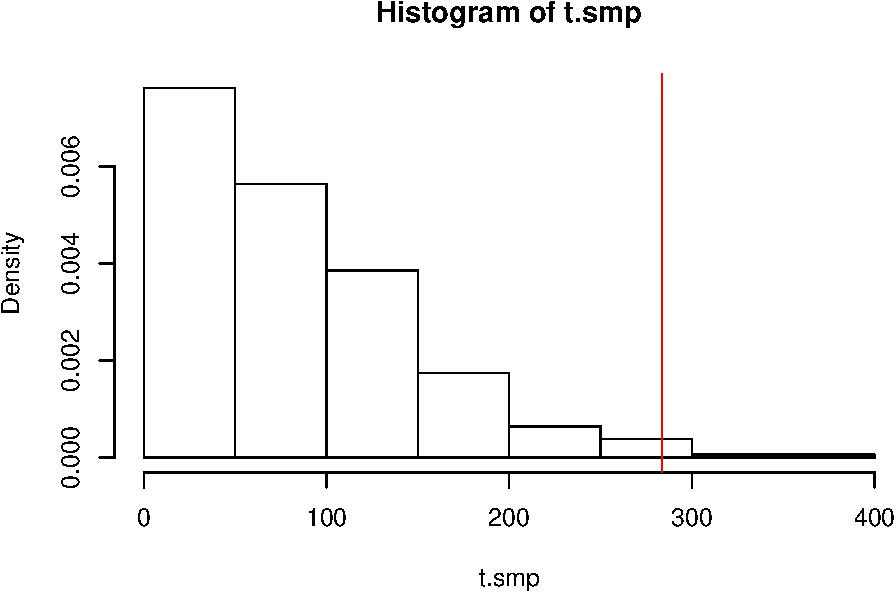
\includegraphics{04-pca_files/figure-latex/unnamed-chunk-24-1.pdf}

We might interpret the PCs as follows. The first PC seems to measure the difference in goals scored and conceded between teams. Low values of PC1 indicate good peformance, and high values poor performance. Teams are rewarded with -0.79 for each positive goal difference, and -0.5 for each goal scored, whilst being penalised by 0.28 for every goal they concede. So a team with a large negative PC1 score tends to score lots of goals and concede few. If we rank teams by their PC1 score, and compare this with the rankings using 3 points for a win and 1 point for a draw we get a different ranking of the teams.

\begin{tabular}{lrr}
\toprule
  & PC1 & PC2\\
\midrule
Manchester City & -85.59 & 12.35\\
Liverpool & -67.64 & 0.93\\
Manchester United & -36.66 & -7.73\\
Leicester City & -32.16 & -1.13\\
Chelsea & -21.19 & 10.90\\
\bottomrule
\end{tabular}

The second PC has a strong positive loading for both goals for and against. A team with a large positive PC 2 score was, therefore, involved in matches with lots of goals. We could, therefore, interpret PC 2 as an `entertainment' measure, ranking teams according to their involvement in high-scoring games.

The above example raises the question of how many PCs should we use in practice. If we reduce the dimension to \(p=1\) then we can rank observations and analyse our new variable with univariate statistics. If we reduce the dimension to \(p=2\) then it is still easy to visualise the data. However, reducing the dimension to \(p=1\) or \(p=2\) may involve losing lots of information and a sensible answer should depend on the objectives of the analysis and the data itself.

The scree graph for the football example is:

\includegraphics{04-pca_files/figure-latex/unnamed-chunk-27-1.pdf}

There are many possible methods for choosing the number of PCs to retain for analysis, including:

\begin{itemize}
\tightlist
\item
  retaining enough PCs to explain, say, 90\% of the total variation;
\item
  retaining PCs where the eigenvalue is above the average.
\end{itemize}

To retain enough PCs to explain 90\% of the total variance, would require us to keep just a single PCs in this case.

\subsection{\texorpdfstring{PCA based on \(\mathbf R\) versus PCA based on \(\mathbf S\)}{PCA based on \textbackslash mathbf R versus PCA based on \textbackslash mathbf S}}\label{pcawithR}

Recall the distinction between the sample covariance matrix \(\mathbf S\) and the sample correlation matrix \(\mathbf R\).
Note that all correlation matrices are also covariance matrices, but not all covariance matrices are correlation matrices.
Before doing PCA we must decide whether to do PCA based on \(\mathbf S\) or \(\mathbf R\)? As we will see later

\begin{itemize}
\tightlist
\item
  PCA based on \(\mathbf R\) (but not \(\mathbf S\)) is scale invariant, whereas
\item
  PCA based on \(\mathbf S\) is invariant under orthogonal rotation.
\end{itemize}

If the original \(p\) variables represent very different types of quantity or show marked differences in variances, then it will usually be better to use \(\mathbf R\) rather than \(\mathbf S\). However, in some circumstances, we may wish to use \(\mathbf S\), such as when the \(p\) variables are measuring similar entities and the sample variances are not too different.

Given that the required numerical calculations are easy to perform in R, we might wish to do it both ways and see if it makes much difference. To use the correlation matrix \(\mathbf R\), we just add the option \texttt{scale=TRUE} when using the \texttt{prcomp} command. Note that \texttt{prcomp} uses \(n-1\) when computing the covariance matrix, rather than \(n\).

\subsubsection{Football example continued}\label{football-example-continued}

If we repeat the analysis of the football data using \(\mathbf R\) instead of \(\mathbf S\), we get find principal components:

\begin{align*}
\boldsymbol \Lambda&= \text{diag}\begin{pmatrix}4.51&1.25&0.156&0.0863&3.68e-32&2.48e-33 \\\end{pmatrix}\\
\;\\
\mathbf V= [\mathbf v_1 \ldots \mathbf v_6] &=\begin{pmatrix}-0.456&0.149&-0.342&-0.406&0.466&0.52 \\0.143&-0.844&0.344&-0.143&0.24&0.268 \\0.432&0.321&0.186&0.541&0.413&0.461 \\-0.438&0.214&0.7&-0.0181&0.389&-0.348 \\0.419&0.342&0.386&-0.671&-0.245&0.22 \\-0.466&-0.00136&0.302&0.269&-0.586&0.525 \\\end{pmatrix}
\end{align*}

The effect of using \(\mathbf R\) is to standardize each of the original variables to have variance 1.
The first PC now has loadings which are more evenly balanced across the 6 original variables.

Teams will have a small value of PC1 score if they won lots, lost rarely, scored a lot, and conceded rarely. In other words, PC1 is a complete measure of overall performance. If we look at the league table based on ordering according to PC1 we get a table that looks more like the original table.

\begin{tabular}{lrr}
\toprule
  & PC1 & PC2\\
\midrule
Liverpool & -4.70 & 1.20\\
Manchester City & -4.38 & 1.65\\
Manchester United & -2.01 & -1.29\\
Chelsea & -1.29 & 1.08\\
Leicester City & -1.66 & 0.12\\
\addlinespace
Tottenham Hotspur & -0.91 & -0.65\\
Wolverhampton & -0.82 & -1.88\\
Arsenal & -0.46 & -1.56\\
Sheffield United & -0.18 & -1.38\\
Burnley & 0.18 & -0.10\\
\bottomrule
\end{tabular}

Overall for these data, doing PCA with \(\mathbf R\) instead of \(\mathbf S\) better summarizes the data (although this is just my subjective opinion - you may feel differently).

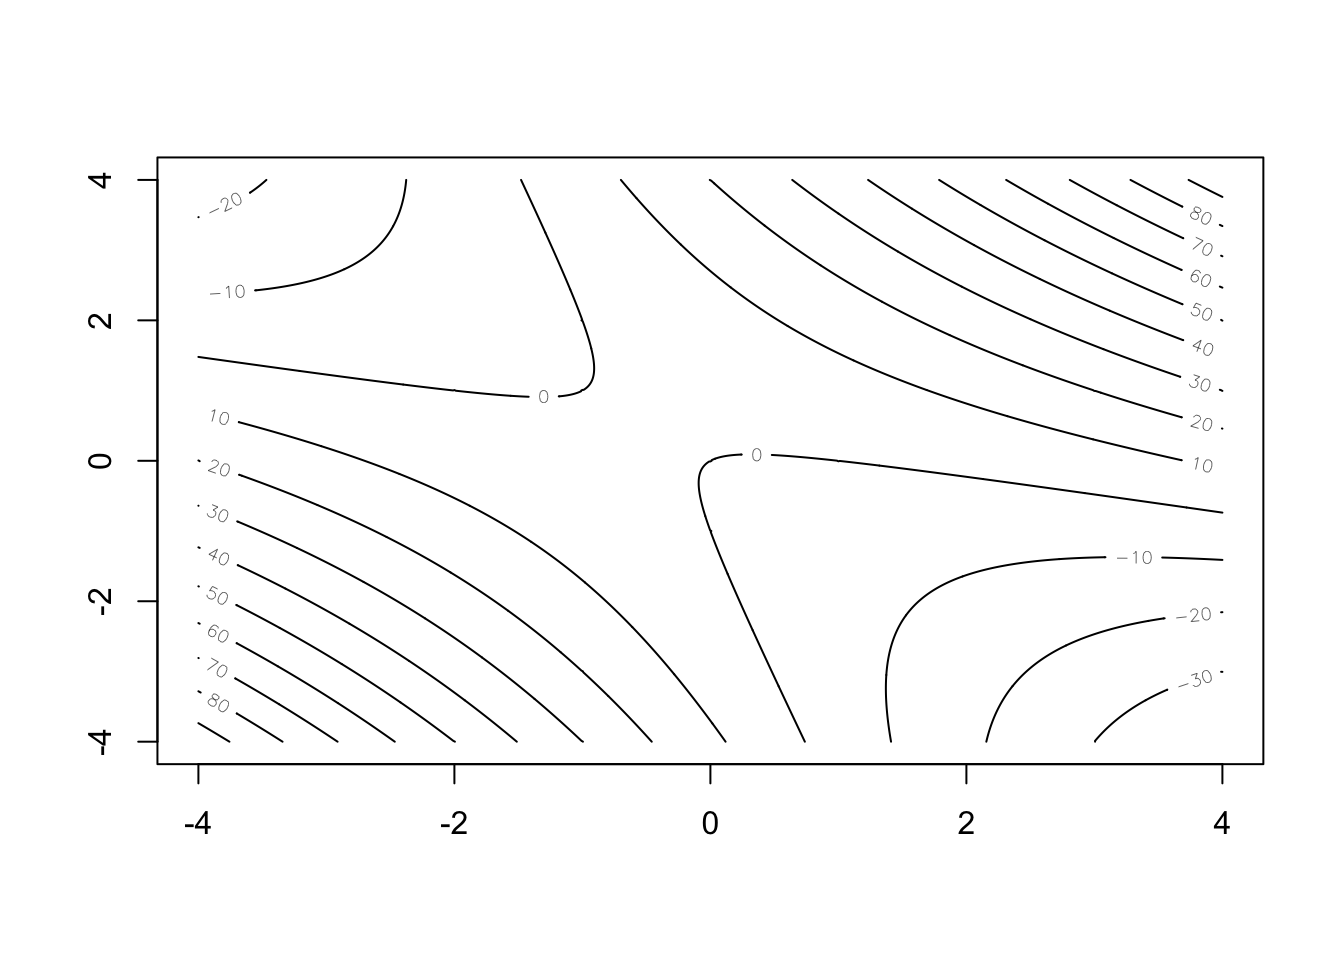
\includegraphics{04-pca_files/figure-latex/unnamed-chunk-30-1.pdf}

\subsection{Population PCA}\label{population-pca}

So far we have considered sample PCA based on the sample covariance matrix or sample correlation matrix:
\[
\mathbf S=\frac{1}{n}\sum_{i=1}^n (\mathbf x_i-\bar{\mathbf x})(\mathbf x_i-\bar{\mathbf x})^\top.
\]

We note now that there is a \emph{population} analogue of PCA based on the population
covariance matrix \(\boldsymbol{\Sigma}\). Although the population version of PCA is not of as much direct practical
relevance as sample PCA, it is nevertheless of conceptual importance.

Let \(\mathbf x\) denote a \(p \times 1\) random vector with \({\mathbb{E}}(\mathbf x)={\pmb \mu}\) and \({\mathbb{V}\operatorname{ar}}(\mathbf x)={\pmb \Sigma}\). As defined,
\(\pmb \mu\) is the population mean vector and \(\pmb \Sigma\) is the population covariance matrix.

Since \(\pmb \Sigma\) is symmetric, the spectral decomposition theorem tells us that
\[
{\pmb \Sigma}=\sum_{j=1}^p \check{\lambda}_j \check{\mathbf v}_j \check{\mathbf v}_j^\top=\check{\mathbf V} \check{\boldsymbol \Lambda}\check{\mathbf V}^\top
\]
where the `check' symbol \(\quad \check{} \quad\) is used to distinguish population quantities from their sample analogues.

Then:

\begin{itemize}
\tightlist
\item
  the first population PC is defined by \(Y_1=\check{\mathbf v}_1^\top (\mathbf x-{\pmb \mu})\);
\item
  the second population PC is defined by \(Y_2=\check{\mathbf v}_2^\top (\mathbf x-{\pmb \mu})\);
\item
  \(\ldots\)
\item
  the \(p\)th population PC is defined by \(Y_p=\check{\mathbf v}_p^\top (\mathbf x-{\pmb \mu})\).
\end{itemize}

The \(Y_1, \ldots , Y_p\) are random variables, unlike the sample PCA case, where the \(y_{ij}\) are observed quantities.
In the sample PCA case, the \(y_{ij}\) can often be regarded as the observed values of random variables.

In matrix form, the above definitions can be summarised by writing
\[
\mathbf y=\begin{pmatrix} Y_1 \\ Y_2 \\ ... \\...\\Y_p   \end{pmatrix} = \check{\mathbf V}^\top (\mathbf x-{\pmb \mu}).
\]

The population PCA analogues of the sample PCA properties listed in Proposition \ref{prp:pca2} are now given. Note that the
\(Y_j\)'s are random variables as opposed to observed values of random variables.

\begin{proposition}
\protect\hypertarget{prp:pca3}{}\label{prp:pca3}

The following results hold for the random variables \(Y_1, \ldots , Y_p\) defined above.

\begin{enumerate}
\def\labelenumi{\arabic{enumi}.}
\item
  \({\mathbb{E}}(Y_j)=0\) for \(j=1, \ldots , p\);
\item
  \({\mathbb{V}\operatorname{ar}}(Y_j)=\check{\lambda}_j\) for \(j=1,\ldots, p\);
\item
  \({\mathbb{C}\operatorname{ov}}(Y_j,Y_k)=0\) if \(j \neq k\);
\item
  \({\mathbb{V}\operatorname{ar}}(Y_1) \geq {\mathbb{V}\operatorname{ar}}(Y_2) \geq \cdots \geq {\mathbb{V}\operatorname{ar}}(Y_p) \geq 0\);
\item
  \(\sum_{j=1}^p {\mathbb{V}\operatorname{ar}}(Y_j)=\sum_{j=1}^p \check{\lambda}_j=\text{tr}(\boldsymbol{\Sigma})\);
\item
  \(\prod_{j=1}^p \text{Var}(Y_j)=\prod_{j=1}^p \check{\lambda}_j=\vert \boldsymbol{\Sigma}\vert\).
\end{enumerate}

\end{proposition}

Note that, defining \(\mathbf y=(Y_1, \ldots , Y_p)^\top\) as before, part 1. implies that \({\mathbb{E}}(\mathbf y)={\mathbf 0}_p\) and parts 2. and 3. together imply that
\[
\text{Var}(\mathbf y)=\boldsymbol \Lambda\equiv \text{diag}(\check{\lambda}_1, \ldots , \check{\lambda}_p).
\]

Consider now a repeated sampling framework in which we assume that \(\mathbf x_1, \ldots , \mathbf x_n\) are IID random vectors from a population
with mean vector \(\pmb \mu\) and covariance matrix \(\boldsymbol{\Sigma}\).

What is the relationship between the sample PCA based on the sample of observed vectors \(\mathbf x_1, \ldots , \mathbf x_n\), and the population PCA based on the unobserved random vector \(\mathbf x\),
from the same population?

If the elements of \(\boldsymbol{\Sigma}\) are all finite, then as \(n\) increases, the elements of the sample covariance matrix \(\mathbf S\) will converge to the corresponding elements
of the population covariance matrix \(\boldsymbol{\Sigma}\). Consequently, we expect the principal components from sample PCA to converge to the population PCA values as \(n\) grows large. Justification of this statement comes from the weak law of large numbers applied to the components of \(\boldsymbol{\Sigma}\), but the details are beyond the scope of this module.

\subsection{PCA under transformations of variables}\label{pca-under-transformations-of-variables}

We'll now consider what happens to PCA when the data are transformed in various ways.

\textbf{Addition transformation}

Firstly, consider the transformation of addition where, for example, we add a fixed amount to each variable.
We can write this transformation as \(\mathbf z_i = \mathbf x_i + \mathbf c\), where \(\mathbf c\) is a fixed vector. Under this transformation the sample mean changes, \(\bar{\mathbf z} = \bar{\mathbf x} + \mathbf c\), but the sample variance remains \(\mathbf S\). Consequently, the eigenvalues and eigenvectors remain the same and, therefore, so do the principal component scores/transformed variables,
\[\mathbf y_i = \mathbf V^\top (\mathbf z_i - \bar{\mathbf z}) = \mathbf V^\top(\mathbf x_i + \mathbf c- (\bar{\mathbf x} + \mathbf c)) = \mathbf V^\top (\mathbf x_i - \bar{\mathbf x}).\]
We say that the principal components are \textbf{invariant} under the addition transformation. An important special case is to choose \(\mathbf c= -\bar{\mathbf x}\) so that the PC scores are simply \(\mathbf y_i = \mathbf V^\top \mathbf z_i\).

\textbf{Scale transformation}

Secondly, we consider the scale transformation where each variable is multiplied by a fixed amount.
A scale transformation occurs more naturally when we convert units of measurement from, say, metres to kilometres. We can write this transformation as \(\mathbf z_i = \mathbf D\mathbf x_i\), where \(\mathbf D\) is a diagonal matrix with positive elements. Under this transformation the sample mean changes from \(\bar{\mathbf x}\) to \(\bar{\mathbf z} = \mathbf D\bar{\mathbf x}\), and the sample covariance matrix changes from \(\mathbf S\) to \(\mathbf D\mathbf S\mathbf D\). Consequently, the principal components also change.

This lack of scale-invariance is undesirable. For example, if we analysed data that included some information on distances, we don't want the answer to depend upon whether we use km, metres, or miles as the measure of distance.
One solution is to scale the data using
\[
\mathbf D= \text{diag}(s_{11}^{-1/2}, \ldots , s_{pp}^{-1/2}),
 \]
where \(s_{ii}\) is the \(i\)th diagonal element of \(\mathbf S\). In effect, we have standardised all the new variables to have variance 1. In this case the sample covariance matrix of the \(\mathbf z_i\)'s is simply the sample correlation matrix \(\mathbf R\) of the original variables, \(\mathbf x_i\). Therefore, we can carry out PCA on the sample correlation matrix, \(\mathbf R\), which is invariant to changes of scale.

In summary: \(\mathbf R\) is scale-invariant while \(\mathbf S\) is not. To do PCA on \(\mathbf R\) in R we use the option \texttt{scale=TRUE} in the \texttt{prcomp} command.

We saw an example of this in section \ref{pcawithR} with the football data. Because the sample
variances of \(G\) and \(GA\) are much larger than the sample variances of \(W\), \(D\) and \(L\), doing PCA with \(\mathbf R\) instead of \(\mathbf S\) completely changed the analysis.

\textbf{Orthogonal transformations}

Thirdly, we consider a transformation by an orthogonal matrix, \(\stackrel{p \times p}{\mathbf A}\), such that \(\mathbf A\mathbf A^\top = \mathbf A^\top \mathbf A= \mathbf I_p\), and write \(\mathbf z_i = \mathbf A\mathbf x_i\). This is equivalent to rotating and/or reflecting the original data.

Let \(\mathbf S\) be the sample covariance matrix of the \(\mathbf x_i\) and let \(\mathbf T\) be the sample covariance matrix of the \(\mathbf z_i\). Under this transformation the sample mean changes from \(\bar{\mathbf x}\) to \(\bar{\mathbf z} = \mathbf A\bar{\mathbf x}\), and the sample covariance matrix \(\mathbf S\) changes from \(\mathbf S\) to \(\mathbf T= \mathbf A\mathbf S\mathbf A^\top\).

However, if we write \(\mathbf S\) in terms of its spectral decomposition \(\mathbf S= \mathbf V\boldsymbol \Lambda\mathbf V^\top\), then \(\mathbf T= \mathbf A\mathbf V\boldsymbol \Lambda\mathbf V^\top \mathbf A^\top = \mathbf B\boldsymbol \Lambda\mathbf B^\top\) where \(\mathbf B= \mathbf A\mathbf V\) is also orthogonal. It is therefore apparent that the eigenvalues of \(\mathbf T\) are the same as those of \(\mathbf S\); and the eigenvectors of \(\mathbf T\) are given by \(\mathbf b_j\) where \(\mathbf b_j = \mathbf A\mathbf v_j\), \(j=1,\ldots,p\). The PC scores of the rotated variables are
\[ \mathbf y_i = \mathbf B^\top (\mathbf z_i - \bar{\mathbf z}) = \mathbf V^\top \mathbf A^\top \mathbf A(\mathbf x_i - \bar{\mathbf x}) = \mathbf V^\top (\mathbf x_i - \bar{\mathbf x}),\]
and so they are identical to the PC scores of the original variables.

Therefore, under an orthogonal transformation the eigenvalues and PC scores are unchanged; the PCs are orthogonal transformations of the original PCs. We say that the principal components are \textbf{equivariant} with respect to orthogonal transformations.

\section{An alternative view of PCA}\label{an-alternative-view-of-pca}

In this section, we will again consider the situation in which the sample \(\mathbf x_1, \ldots ,  \mathbf x_n \in \mathbb{R}^p\) have zero mean (replace \(\mathbf x_i\) by \(\mathbf x_i-\bar{\mathbf x}\) if the mean is not zero).

To recap, in PCA to find the \(r\) leading principal components, we solve the optimization problem
\begin{align*}
\mbox{For } k=1, \ldots, r &\mbox{ maximize } \mathbf u_k^\top \mathbf S\mathbf u_k \\
 &\mbox{ subject to } \mathbf u_k^\top \mathbf u_j = \begin{cases}
 1  &\mbox{ if } j=k\\
 0 & \mbox{ otherwise.}
 \end{cases}
 \end{align*}

We can write this in the form given in the introduction to this chapter (Equation \eqref{eq:dimredopt}) as
\begin{align*}
&\mbox{Maximize } \operatorname{tr}(\mathbf U^\top \mathbf S\mathbf U) \\
 &\mbox{ subject to } \mathbf U^\top \mathbf U=\mathbf I_r,
 \end{align*}
as \(\operatorname{tr}(\mathbf U^\top \mathbf S\mathbf U) = \sum_{k=1}^r \mathbf u_k^\top \mathbf S\mathbf u_k\) if \(\mathbf U\) has columns \(\mathbf u_1, \ldots, \mathbf u_r\).

\subsubsection*{An equivalent problem}\label{an-equivalent-problem}
\addcontentsline{toc}{subsubsection}{An equivalent problem}

There is another optimization problem that we sometimes wish to solve, that turns out to be equivalent to the above, thus providing another reason why PCA is so widely used.

Suppose we want to find the best rank-\(r\) linear approximation to the data matrix \(\mathbf X=\begin{pmatrix}\mathbf x_1& \ldots & \mathbf x_n\end{pmatrix}^\top\) (remember that we're assuming the data have been column centered, if not, replace \(\mathbf X\) by \(\mathbf H\mathbf X\)). One way to think about this is seek a \(p\times r\) matrix \(\mathbf U\) for which the rank \(r\) linear model
\[f(\mathbf y) = \mathbf U\mathbf y\] can be used to represent the data.

Let's choose \(\mathbf y_i\in \mathbb{R}^r\) and \(\mathbf U\) to minimize the sum of squared errors
\[\sum_{i=1}^n ||\mathbf x_i - \mathbf U\mathbf y_i||^2_2.\]

If we write
\[\mathbf Y^\top = \begin{pmatrix} 
| &&|\\
\mathbf y_1& \ldots & \mathbf y_n\\
| &&|
\end{pmatrix}\]
then
\begin{align*}
\sum_{i=1}^n ||\mathbf x_i - \mathbf U\mathbf y_i||^2_2 &=\operatorname{tr}((\mathbf X^\top - \mathbf U\mathbf Y^\top)^\top (\mathbf X^\top - \mathbf U\mathbf Y^\top))\\
&=||\mathbf X^\top - \mathbf U\mathbf Y^\top||_F^2
\end{align*}

i.e., we're looking for the rank-\(r\) matrix \(\mathbf X_r\) that minimizes \(||\mathbf X- \mathbf X_r||_F=||\mathbf X^\top - \mathbf X_r^\top||_F\), noting that we can write an arbitrary rank-\(r\) matrix as \(\mathbf X_r^\top = \mathbf U\mathbf Y^\top\) for some \(p\times r\) matrix \(\mathbf U\) and a \(n \times r\) matrix \(\mathbf Y\).

It makes sense to restrict the columns of \(\mathbf U\) to be orthonormal so that \(\mathbf U^\top \mathbf U=\mathbf I_r\) as non-orthonormal coordinates systems are confusing. We know that the \(\mathbf u\in \mathcal{C}(\mathbf U)\) (where \(\mathcal{C}(\mathbf U)\) is the column space of \(\mathbf U\)) that minimizes
\[||\mathbf x-\mathbf u||_2\]
is the orthogonal projection of \(\mathbf x\) onto \(\mathcal{C}(\mathbf U)\), which given the columns of \(\mathbf U\) are orthonormal is \(\mathbf u= \mathbf U\mathbf U^\top \mathbf x\) (see Section \ref{orthogproj}). So we must have \(\mathbf X_r^\top = \mathbf U\mathbf U^\top \mathbf X^\top\) and \(\mathbf Y^\top = \mathbf U^\top \mathbf X^\top\).

So it remains to find the optimal choice for \(\mathbf U\) by minimizing
\begin{align*}
||\mathbf X^\top - \mathbf U\mathbf U^\top \mathbf X^\top||_F^2 &=||\mathbf X- \mathbf X\mathbf U\mathbf U^\top ||_F^2\\
&= \operatorname{tr}((\mathbf X- \mathbf X\mathbf U\mathbf U^\top)^\top(\mathbf X- \mathbf X\mathbf U\mathbf U^\top))\\
&= \operatorname{tr}(\mathbf X^\top \mathbf X) - 2 \operatorname{tr}(\mathbf U\mathbf U^\top \mathbf X^\top\mathbf X) +  \operatorname{tr}(\mathbf U\mathbf U^\top \mathbf X^\top\mathbf X\mathbf U\mathbf U^\top)\\
&= \operatorname{tr}(\mathbf X^\top \mathbf X)  - \operatorname{tr}(\mathbf U^\top \mathbf X^\top \mathbf X\mathbf U) 
\end{align*}
where we've used the fact \(\operatorname{tr}(\mathbf A\mathbf B) = \operatorname{tr}(\mathbf B\mathbf A)\) and that \(\mathbf U^\top \mathbf U=\mathbf I_r\).

Minimizing the equation above with respect to \(\mathbf U\) is equivalent to maximizing
\[\operatorname{tr}(\mathbf U^\top \mathbf S\mathbf U) \]
which is the maximum variance objective we used to introduce PCA.

So to summarize, the optimization problem
\begin{align*}
&\mbox{Minimize } ||\mathbf X^\top -\mathbf U\mathbf U^\top \mathbf X^\top||_F \\
 &\mbox{ subject to } \mathbf U^\top \mathbf U=\mathbf I_r,
 \end{align*}
is equivalent to (and has the same as) the PCA optimization problem.

\subsection{Example: MNIST handwritten digits}\label{pca-mnist}

Let's consider the MNIST dataset of handwritten digits discussed in Chapter \ref{stat-prelim}. Recall this is a collection of 60,000 digits, each of which has been converted to a \(28\times 28\) pixel greyscale image (so \(p=784\)).
I've made a clean version of the dataset available on Moodle, so you can try this analysis for yourself. Let's look at just the 3s. I've created a plotting function \texttt{plot.mnist}, which is in the code file on Moodle.

\begin{Shaded}
\begin{Highlighting}[]
\FunctionTok{load}\NormalTok{(}\AttributeTok{file=}\StringTok{"mnist.rda"}\NormalTok{) }
\FunctionTok{source}\NormalTok{(}\StringTok{\textquotesingle{}mnisttools.R\textquotesingle{}}\NormalTok{)}
\NormalTok{mnist3 }\OtherTok{=}\NormalTok{ mnist}\SpecialCharTok{$}\NormalTok{train}\SpecialCharTok{$}\NormalTok{x[mnist}\SpecialCharTok{$}\NormalTok{train}\SpecialCharTok{$}\NormalTok{y}\SpecialCharTok{==}\DecValTok{3}\NormalTok{,] }\CommentTok{\# select just the 3s}
\FunctionTok{plot.mnist}\NormalTok{(mnist3[}\DecValTok{1}\SpecialCharTok{:}\DecValTok{12}\NormalTok{,]) }\CommentTok{\# plot the first 12 images}
\end{Highlighting}
\end{Shaded}

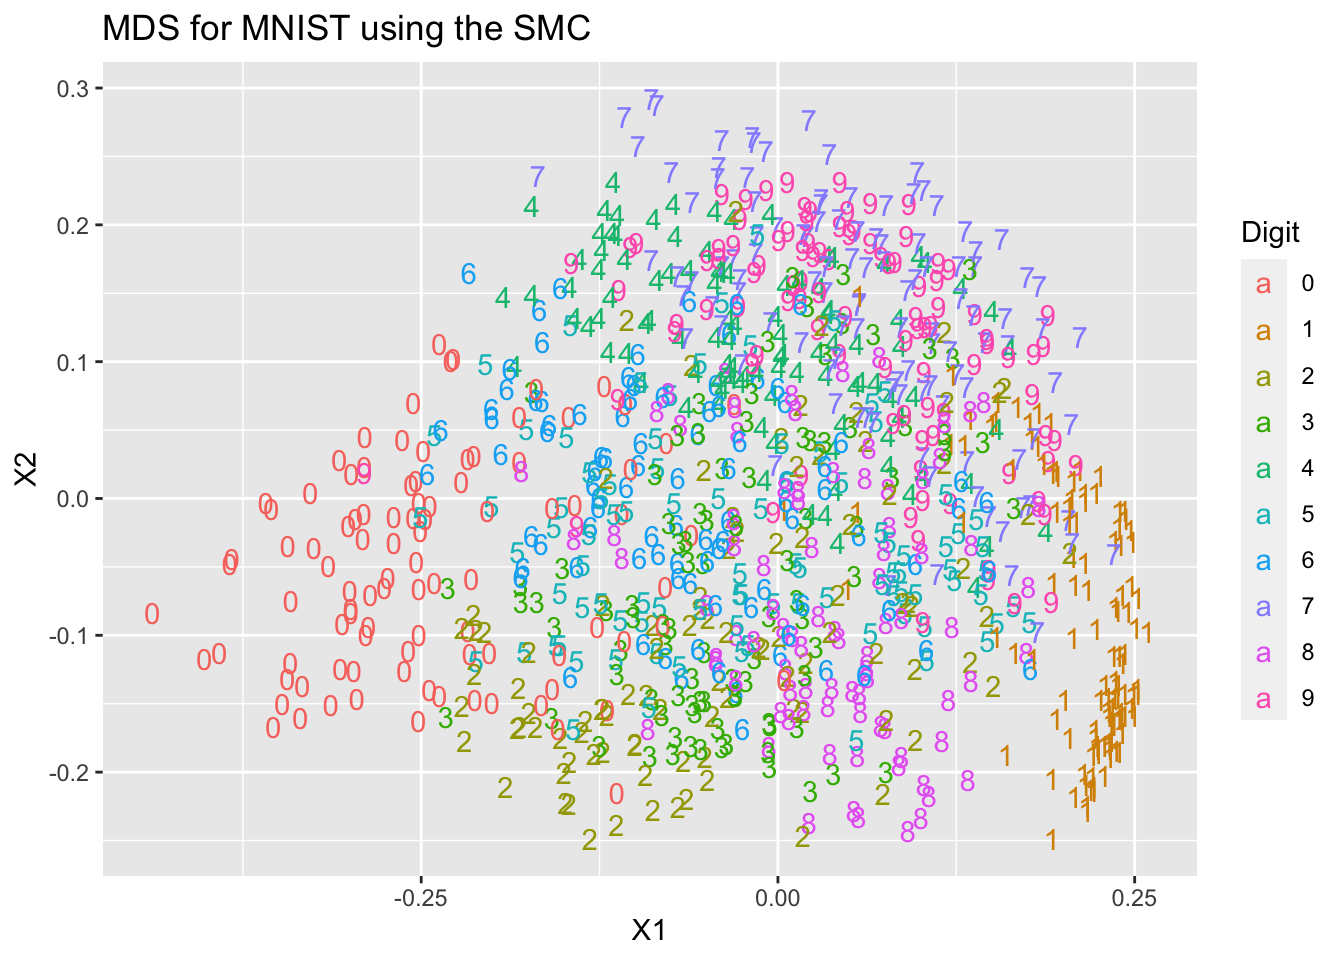
\includegraphics{04-pca_files/figure-latex/unnamed-chunk-31-1.pdf}

We can see there is quite a bit of variation between them.
Now lets look at \(\bar{\mathbf x}\), the average 3.

\begin{Shaded}
\begin{Highlighting}[]
\NormalTok{xbar}\OtherTok{=}\FunctionTok{colMeans}\NormalTok{(mnist3)}
\FunctionTok{plot.mnist}\NormalTok{(xbar)}
\end{Highlighting}
\end{Shaded}

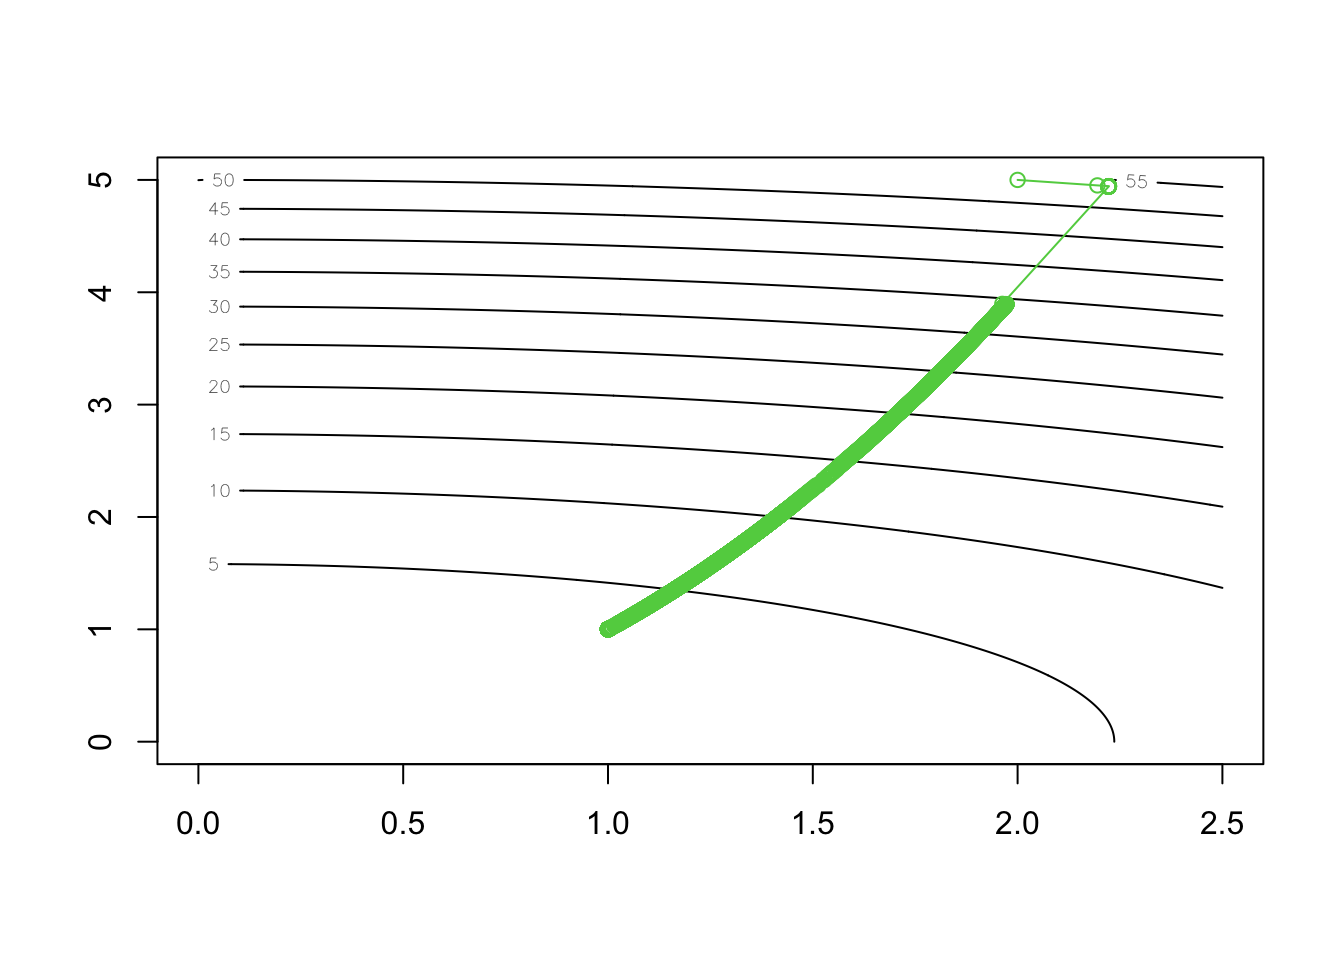
\includegraphics{04-pca_files/figure-latex/unnamed-chunk-32-1.pdf}

We can use the \texttt{prcomp} command to find the principal components. Note that we can't use the \texttt{scale=TRUE} option as some of the columns are all 0, and so R throws an error as it cannot rescale these to have variance 1. Let's plot the first few principal components/eigenvectors/loading vectors.

\begin{Shaded}
\begin{Highlighting}[]
\NormalTok{mnist3.pca }\OtherTok{\textless{}{-}} \FunctionTok{prcomp}\NormalTok{(mnist3)}
\FunctionTok{plot.mnist}\NormalTok{(mnist3.pca}\SpecialCharTok{$}\NormalTok{rotation[,}\DecValTok{1}\SpecialCharTok{:}\DecValTok{12}\NormalTok{]) }
\end{Highlighting}
\end{Shaded}

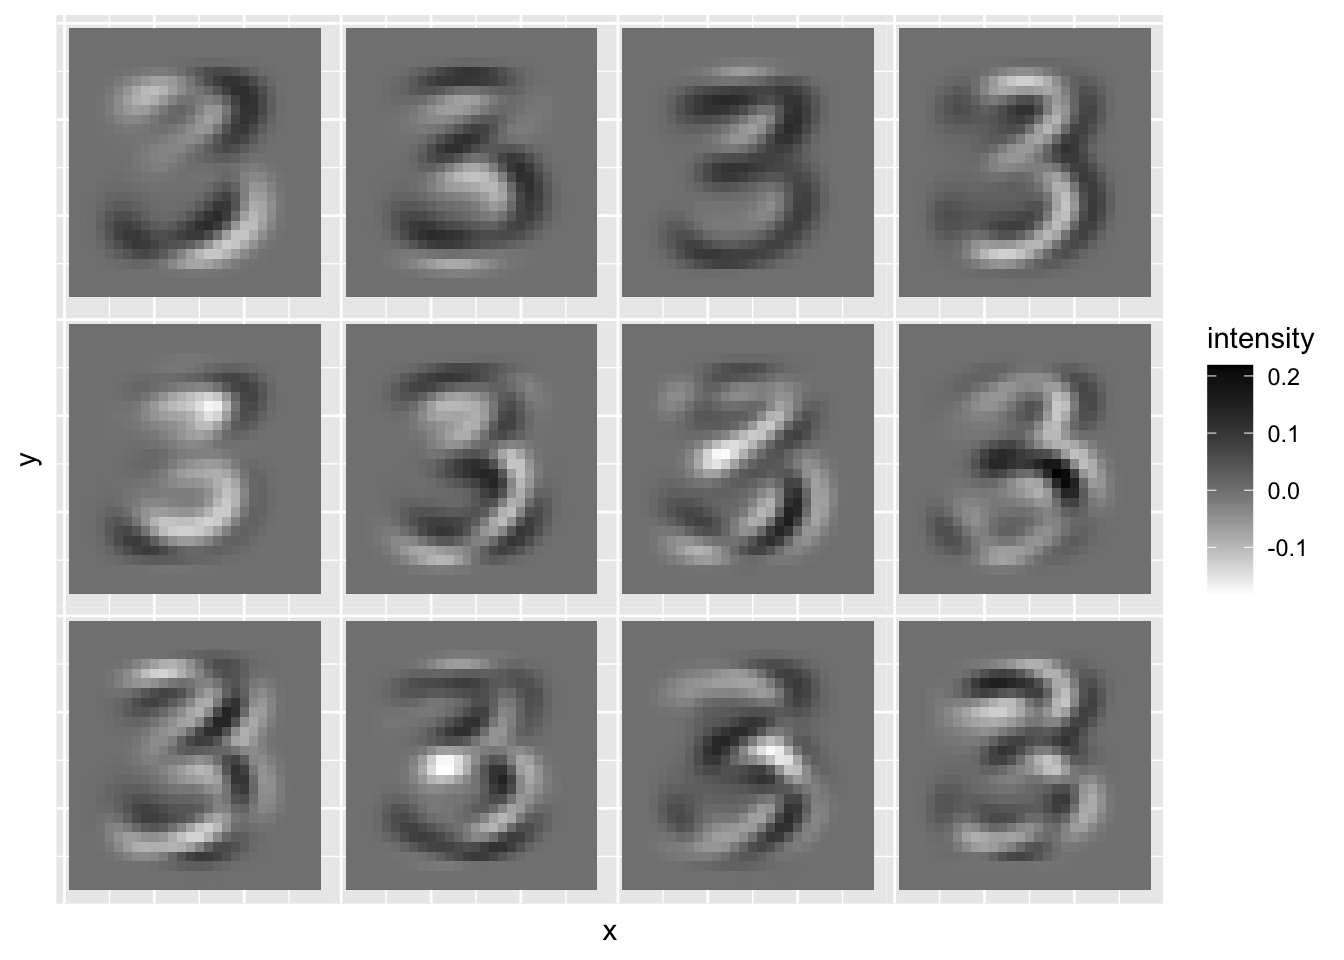
\includegraphics{04-pca_files/figure-latex/unnamed-chunk-33-1.pdf}

These show the main mode of variability in the 3s. Focusing on the first PC, we can see that this is a form of rotation and causes the 3 to slant either forward or backward. If we wanted a rank-2 approximation to the data we would use
\[f(\mathbf y) = \bar{\mathbf x} + y_1 \mathbf v_1 + y_2 \mathbf v_2\]

Let's try reconstructing the data with \(r=2\).

\begin{Shaded}
\begin{Highlighting}[]
\NormalTok{r}\OtherTok{=}\DecValTok{2}
\NormalTok{recon }\OtherTok{=}\NormalTok{  mnist3.pca}\SpecialCharTok{$}\NormalTok{x[,}\DecValTok{1}\SpecialCharTok{:}\NormalTok{r] }\SpecialCharTok{\%*\%} \FunctionTok{t}\NormalTok{(mnist3.pca}\SpecialCharTok{$}\NormalTok{rotation[,}\DecValTok{1}\SpecialCharTok{:}\NormalTok{r])}
\FunctionTok{plot.mnist2}\NormalTok{(}\FunctionTok{matrix}\NormalTok{(}\FunctionTok{rep}\NormalTok{(xbar,}\DecValTok{12}\NormalTok{), }\AttributeTok{byrow=}\NormalTok{T, }\AttributeTok{nr=}\DecValTok{12}\NormalTok{)}\SpecialCharTok{+}\NormalTok{recon[}\DecValTok{1}\SpecialCharTok{:}\DecValTok{12}\NormalTok{,])}
\end{Highlighting}
\end{Shaded}

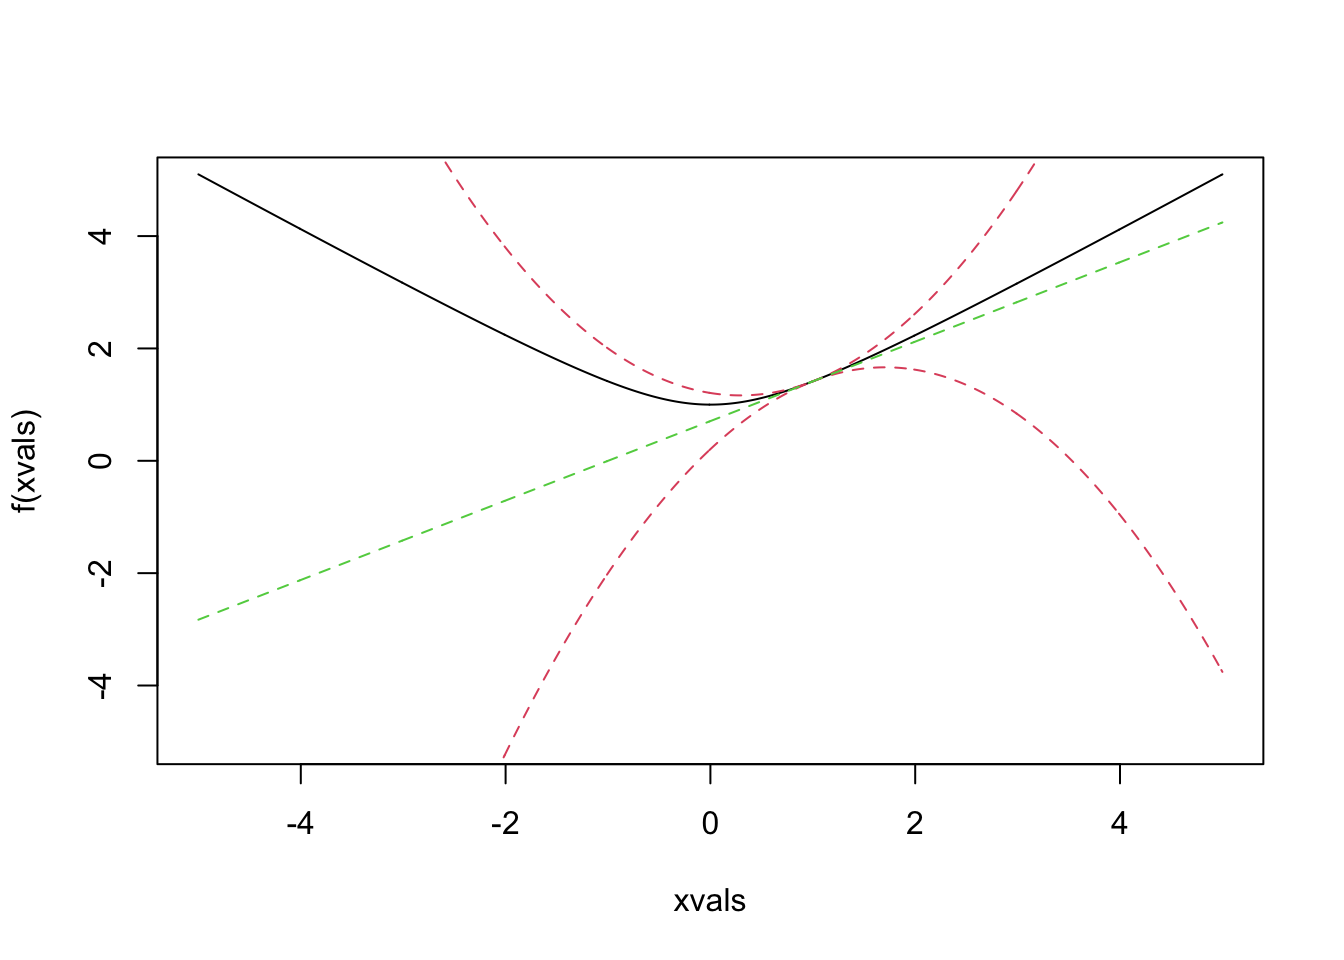
\includegraphics{04-pca_files/figure-latex/unnamed-chunk-34-1.pdf}

We can see that all of these 3s still look a lot like the average 3, but that they vary in their slant, and the heaviness of the line.

The scree plot shows a sharp decrease in the eigenvalues until about the 100th component, at which point they level off.

\begin{Shaded}
\begin{Highlighting}[]
\FunctionTok{plot}\NormalTok{(mnist3.pca}\SpecialCharTok{$}\NormalTok{sdev) }\CommentTok{\# scree plot}
\end{Highlighting}
\end{Shaded}

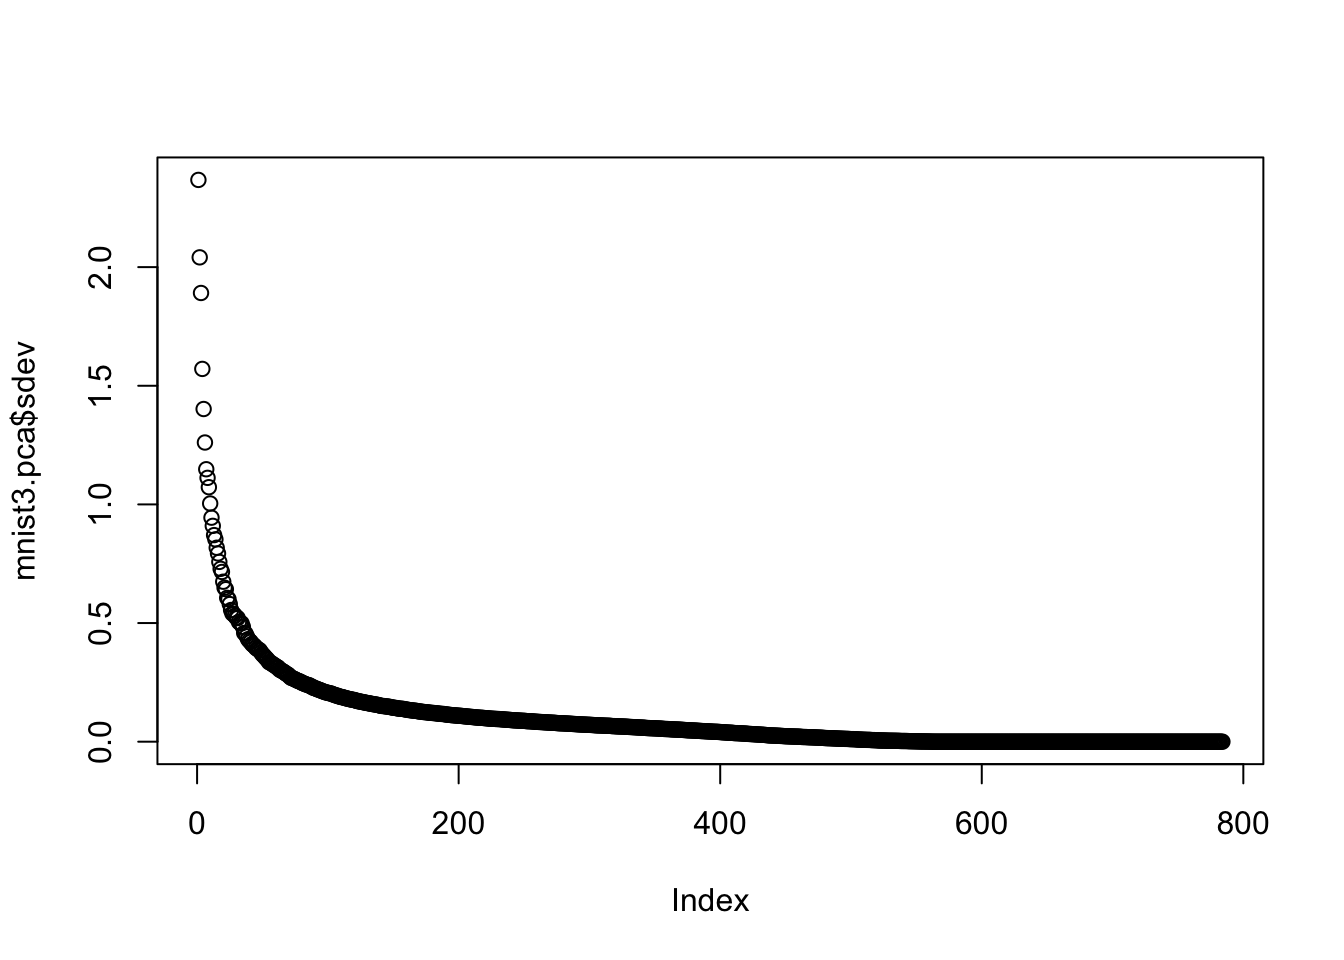
\includegraphics{04-pca_files/figure-latex/unnamed-chunk-35-1.pdf}

It can also be useful to plot the cumulative sum of the total proportion of variance explained by a given number of principal components. I've drawn on horizontal lines at 90\% and 95\% of variance explained, to help identify when we cross these thresholds.
We need 80 components to explain 90\% of the variance, and 138 components to explain 95\% of the variance.

\begin{Shaded}
\begin{Highlighting}[]
\NormalTok{cumvar }\OtherTok{=} \DecValTok{100}\SpecialCharTok{*}\FunctionTok{cumsum}\NormalTok{(mnist3.pca}\SpecialCharTok{$}\NormalTok{sdev}\SpecialCharTok{\^{}}\DecValTok{2}\NormalTok{) }\SpecialCharTok{/} \FunctionTok{sum}\NormalTok{(mnist3.pca}\SpecialCharTok{$}\NormalTok{sdev}\SpecialCharTok{\^{}}\DecValTok{2}\NormalTok{)}
\FunctionTok{plot}\NormalTok{(cumvar, }\AttributeTok{ylab=}\StringTok{"Cumulative proportion of variance explained"}\NormalTok{, }
     \AttributeTok{xlab=}\StringTok{"Number of PCs used"}\NormalTok{, }\AttributeTok{ylim=}\FunctionTok{c}\NormalTok{(}\DecValTok{0}\NormalTok{,}\DecValTok{100}\NormalTok{))}
\FunctionTok{abline}\NormalTok{(}\AttributeTok{h=}\DecValTok{90}\NormalTok{, }\AttributeTok{lty=}\DecValTok{2}\NormalTok{)}
\FunctionTok{abline}\NormalTok{(}\AttributeTok{v=}\FunctionTok{min}\NormalTok{(}\FunctionTok{which}\NormalTok{(cumvar}\SpecialCharTok{\textgreater{}}\DecValTok{90}\NormalTok{)), }\AttributeTok{lty=}\DecValTok{2}\NormalTok{)}
\FunctionTok{abline}\NormalTok{(}\AttributeTok{h=}\DecValTok{95}\NormalTok{, }\AttributeTok{lty=}\DecValTok{2}\NormalTok{)}
\FunctionTok{abline}\NormalTok{(}\AttributeTok{v=}\FunctionTok{min}\NormalTok{(}\FunctionTok{which}\NormalTok{(cumvar}\SpecialCharTok{\textgreater{}}\DecValTok{95}\NormalTok{)), }\AttributeTok{lty=}\DecValTok{2}\NormalTok{)}
\end{Highlighting}
\end{Shaded}

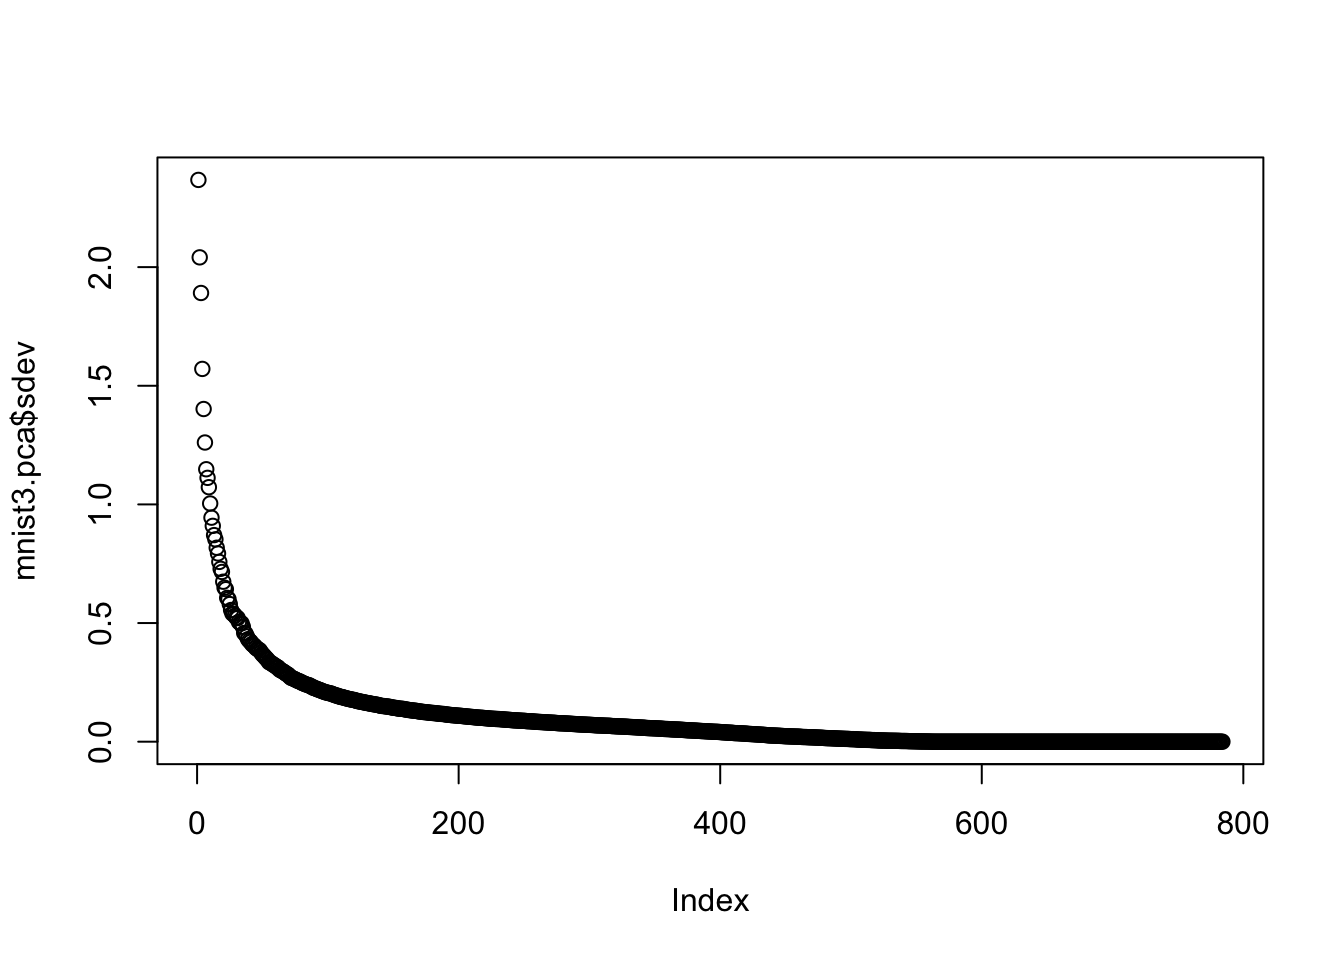
\includegraphics{04-pca_files/figure-latex/unnamed-chunk-37-1.pdf}

Let's now look at the reconstruction using \(r=10, \;50, \;100\) and \(500\) components to see how the accuracy changes.

\begin{Shaded}
\begin{Highlighting}[]
\NormalTok{r}\OtherTok{=}\DecValTok{10}
\NormalTok{recon }\OtherTok{=}\NormalTok{  mnist3.pca}\SpecialCharTok{$}\NormalTok{x[,}\DecValTok{1}\SpecialCharTok{:}\NormalTok{r] }\SpecialCharTok{\%*\%} \FunctionTok{t}\NormalTok{(mnist3.pca}\SpecialCharTok{$}\NormalTok{rotation[,}\DecValTok{1}\SpecialCharTok{:}\NormalTok{r])}
\FunctionTok{plot.mnist2}\NormalTok{(}\FunctionTok{matrix}\NormalTok{(}\FunctionTok{rep}\NormalTok{(xbar,}\DecValTok{12}\NormalTok{), }\AttributeTok{byrow=}\NormalTok{T, }\AttributeTok{nr=}\DecValTok{12}\NormalTok{)}\SpecialCharTok{+}\NormalTok{recon[}\DecValTok{1}\SpecialCharTok{:}\DecValTok{12}\NormalTok{,])}
\end{Highlighting}
\end{Shaded}

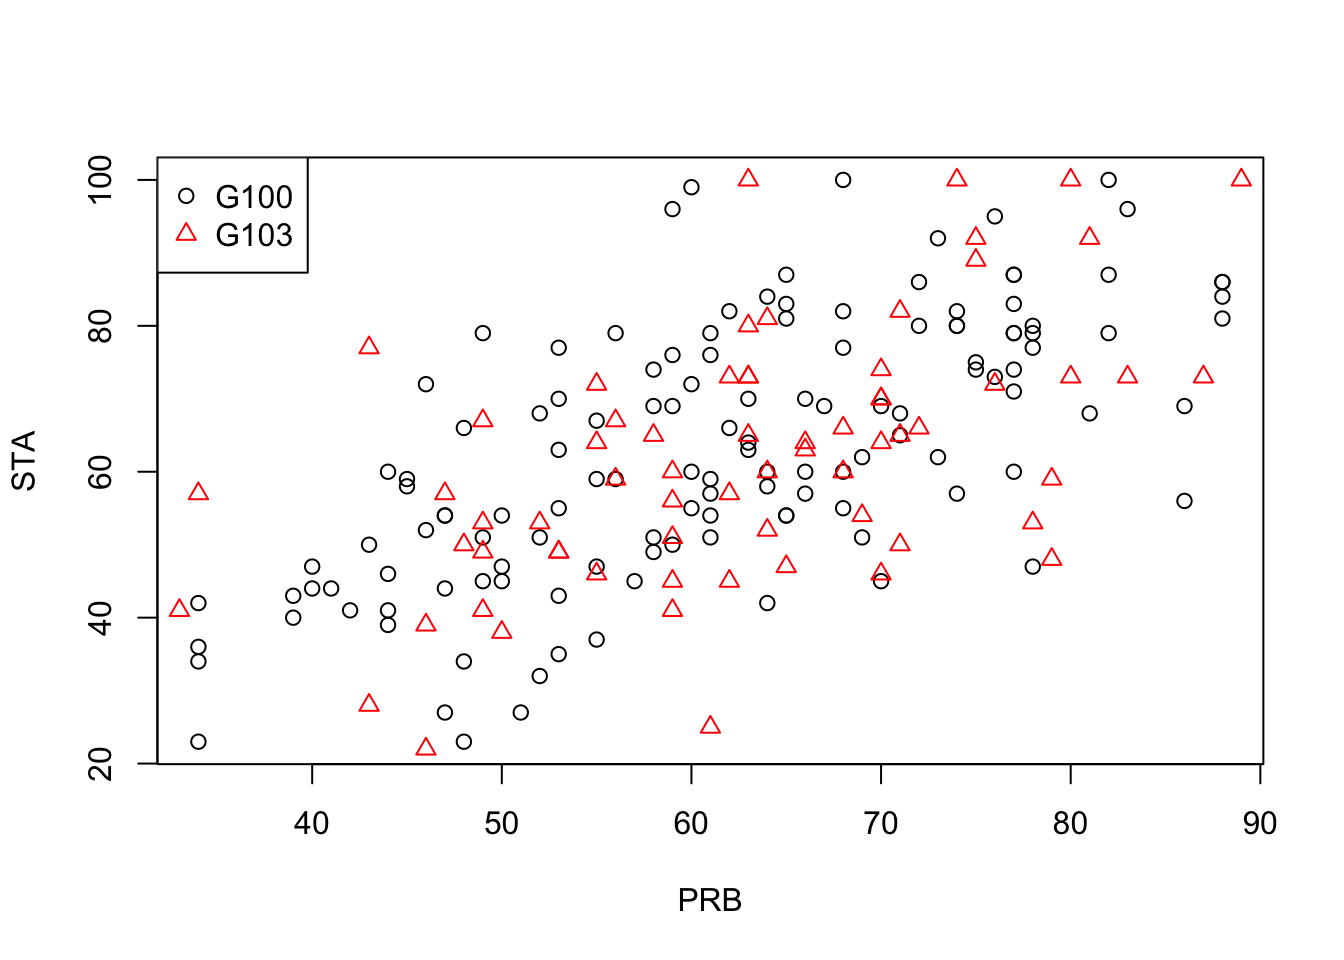
\includegraphics{04-pca_files/figure-latex/unnamed-chunk-38-1.pdf}

\begin{Shaded}
\begin{Highlighting}[]
\NormalTok{r}\OtherTok{=}\DecValTok{50}
\NormalTok{recon }\OtherTok{=}\NormalTok{  mnist3.pca}\SpecialCharTok{$}\NormalTok{x[,}\DecValTok{1}\SpecialCharTok{:}\NormalTok{r] }\SpecialCharTok{\%*\%} \FunctionTok{t}\NormalTok{(mnist3.pca}\SpecialCharTok{$}\NormalTok{rotation[,}\DecValTok{1}\SpecialCharTok{:}\NormalTok{r])}
\FunctionTok{plot.mnist2}\NormalTok{(}\FunctionTok{matrix}\NormalTok{(}\FunctionTok{rep}\NormalTok{(xbar,}\DecValTok{12}\NormalTok{), }\AttributeTok{byrow=}\NormalTok{T, }\AttributeTok{nr=}\DecValTok{12}\NormalTok{)}\SpecialCharTok{+}\NormalTok{recon[}\DecValTok{1}\SpecialCharTok{:}\DecValTok{12}\NormalTok{,])}
\end{Highlighting}
\end{Shaded}

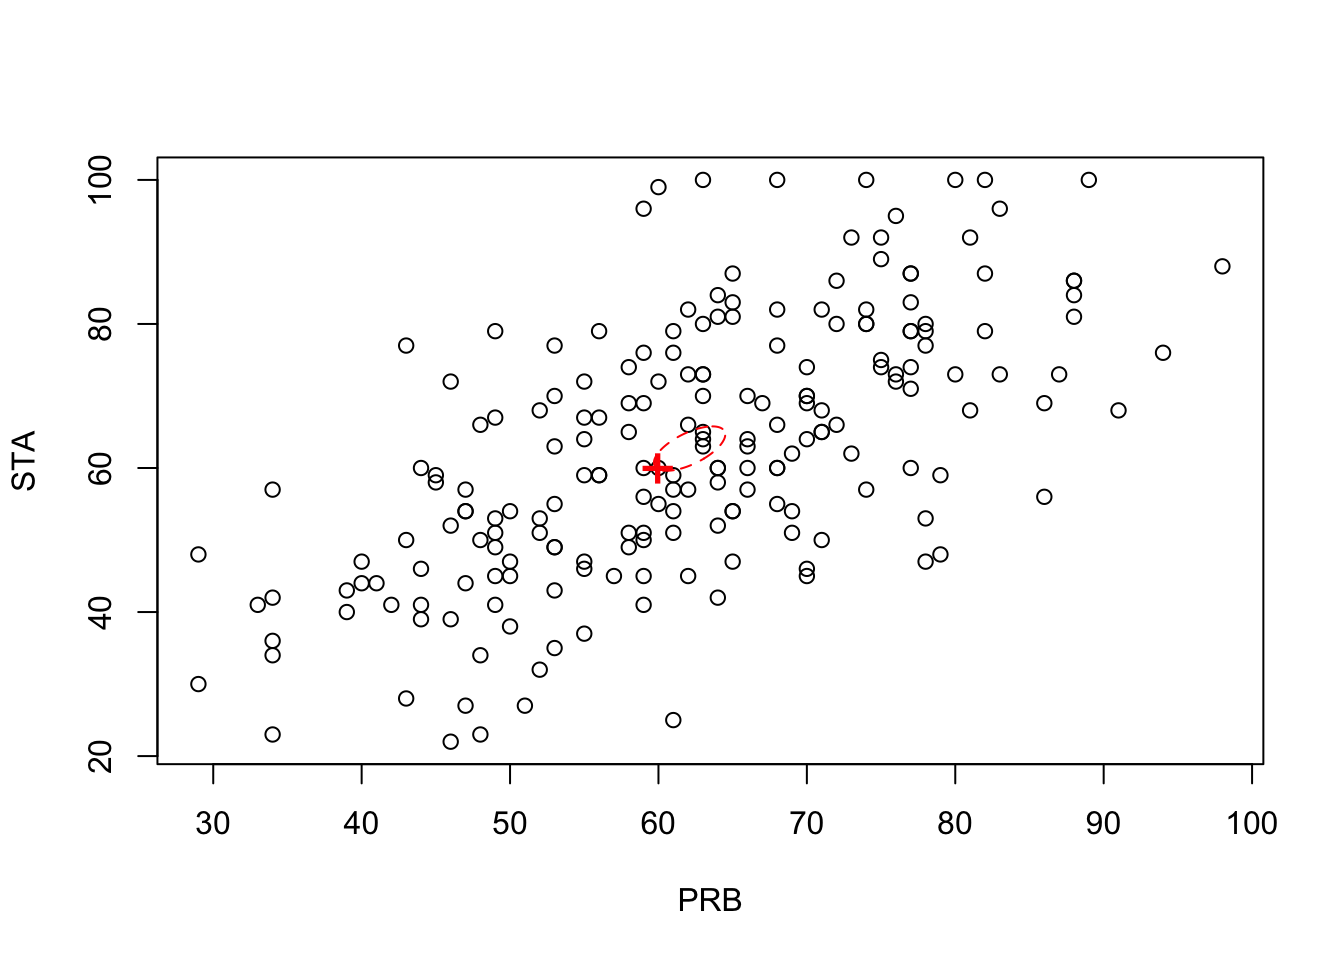
\includegraphics{04-pca_files/figure-latex/unnamed-chunk-39-1.pdf}

\begin{Shaded}
\begin{Highlighting}[]
\NormalTok{r}\OtherTok{=}\DecValTok{100}
\NormalTok{recon }\OtherTok{=}\NormalTok{  mnist3.pca}\SpecialCharTok{$}\NormalTok{x[,}\DecValTok{1}\SpecialCharTok{:}\NormalTok{r] }\SpecialCharTok{\%*\%} \FunctionTok{t}\NormalTok{(mnist3.pca}\SpecialCharTok{$}\NormalTok{rotation[,}\DecValTok{1}\SpecialCharTok{:}\NormalTok{r])}
\FunctionTok{plot.mnist2}\NormalTok{(}\FunctionTok{matrix}\NormalTok{(}\FunctionTok{rep}\NormalTok{(xbar,}\DecValTok{12}\NormalTok{), }\AttributeTok{byrow=}\NormalTok{T, }\AttributeTok{nr=}\DecValTok{12}\NormalTok{)}\SpecialCharTok{+}\NormalTok{recon[}\DecValTok{1}\SpecialCharTok{:}\DecValTok{12}\NormalTok{,])}
\end{Highlighting}
\end{Shaded}

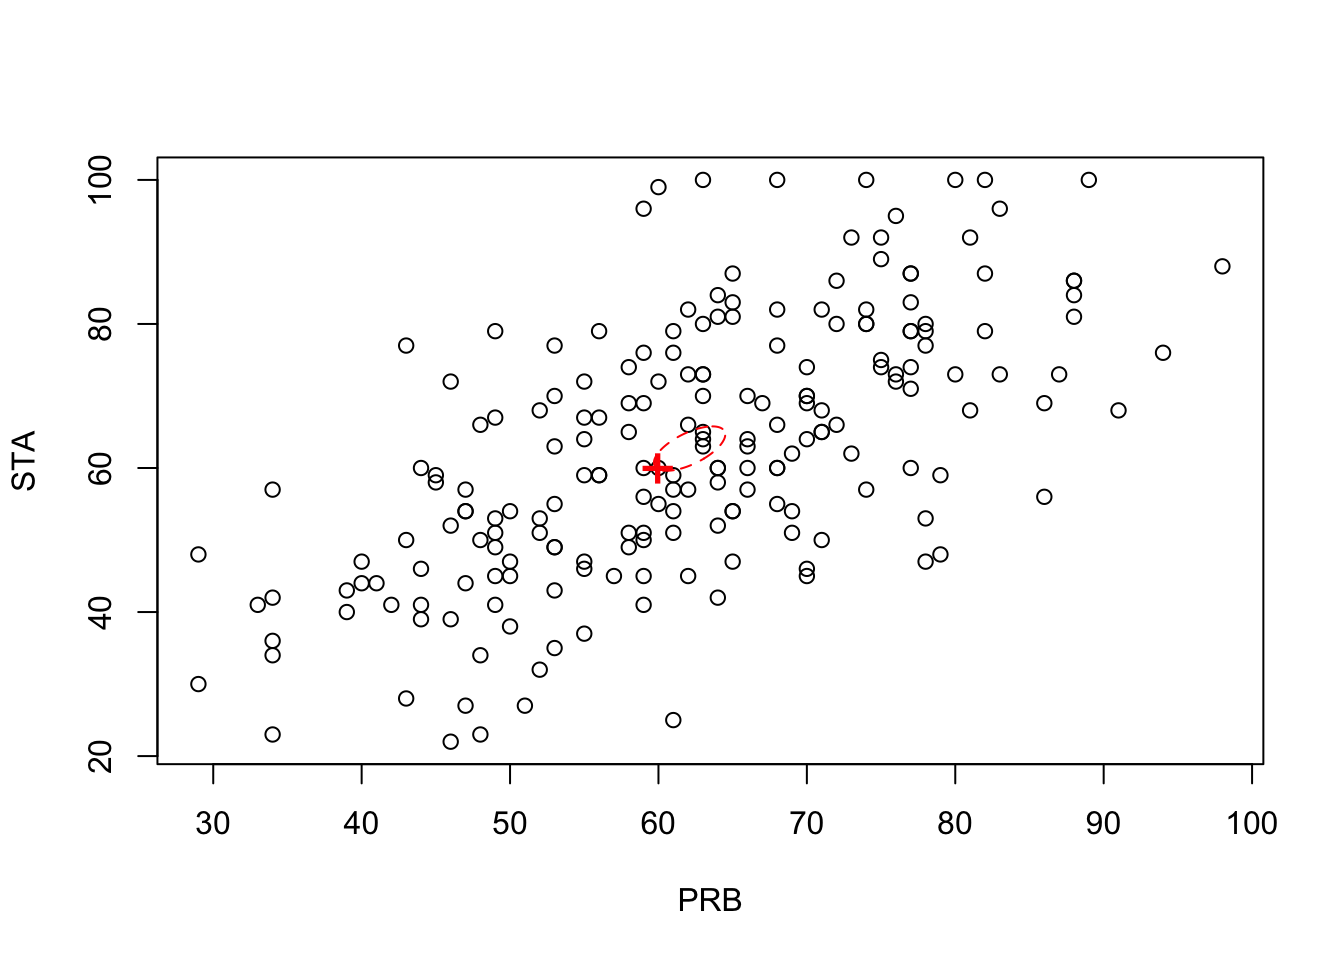
\includegraphics{04-pca_files/figure-latex/unnamed-chunk-40-1.pdf}

\begin{Shaded}
\begin{Highlighting}[]
\NormalTok{r}\OtherTok{=}\DecValTok{500}
\NormalTok{recon }\OtherTok{=}\NormalTok{  mnist3.pca}\SpecialCharTok{$}\NormalTok{x[,}\DecValTok{1}\SpecialCharTok{:}\NormalTok{r] }\SpecialCharTok{\%*\%} \FunctionTok{t}\NormalTok{(mnist3.pca}\SpecialCharTok{$}\NormalTok{rotation[,}\DecValTok{1}\SpecialCharTok{:}\NormalTok{r])}
\FunctionTok{plot.mnist2}\NormalTok{(}\FunctionTok{matrix}\NormalTok{(}\FunctionTok{rep}\NormalTok{(xbar,}\DecValTok{12}\NormalTok{), }\AttributeTok{byrow=}\NormalTok{T, }\AttributeTok{nr=}\DecValTok{12}\NormalTok{)}\SpecialCharTok{+}\NormalTok{recon[}\DecValTok{1}\SpecialCharTok{:}\DecValTok{12}\NormalTok{,])}
\end{Highlighting}
\end{Shaded}

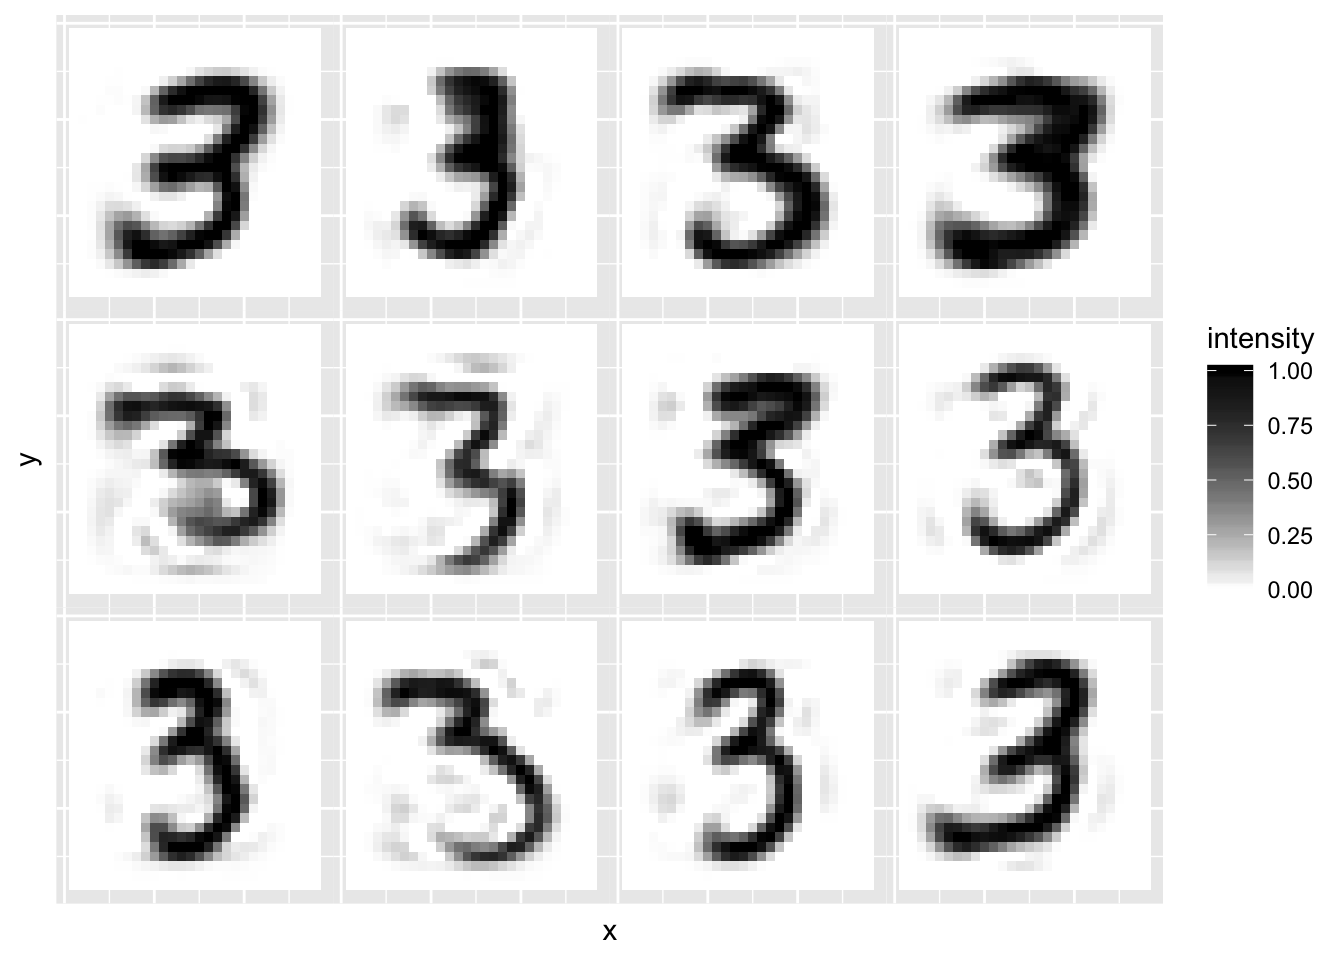
\includegraphics{04-pca_files/figure-latex/unnamed-chunk-41-1.pdf}

We can see that as the number of components increases the reconstructions start to look more like the original 12 images.

We can visualise the range of 3s by looking at a scatter plot of the first two principal components.

\begin{Shaded}
\begin{Highlighting}[]
\FunctionTok{library}\NormalTok{(ggplot2)}
\NormalTok{mnist3.pca}\SpecialCharTok{$}\NormalTok{x}\SpecialCharTok{|\textgreater{}} \FunctionTok{data.frame}\NormalTok{()}\SpecialCharTok{|\textgreater{}} \FunctionTok{ggplot}\NormalTok{(}\FunctionTok{aes}\NormalTok{(}\AttributeTok{x=}\NormalTok{PC1, }\AttributeTok{y=}\NormalTok{PC2))}\SpecialCharTok{+}\FunctionTok{geom\_point}\NormalTok{()}
\end{Highlighting}
\end{Shaded}

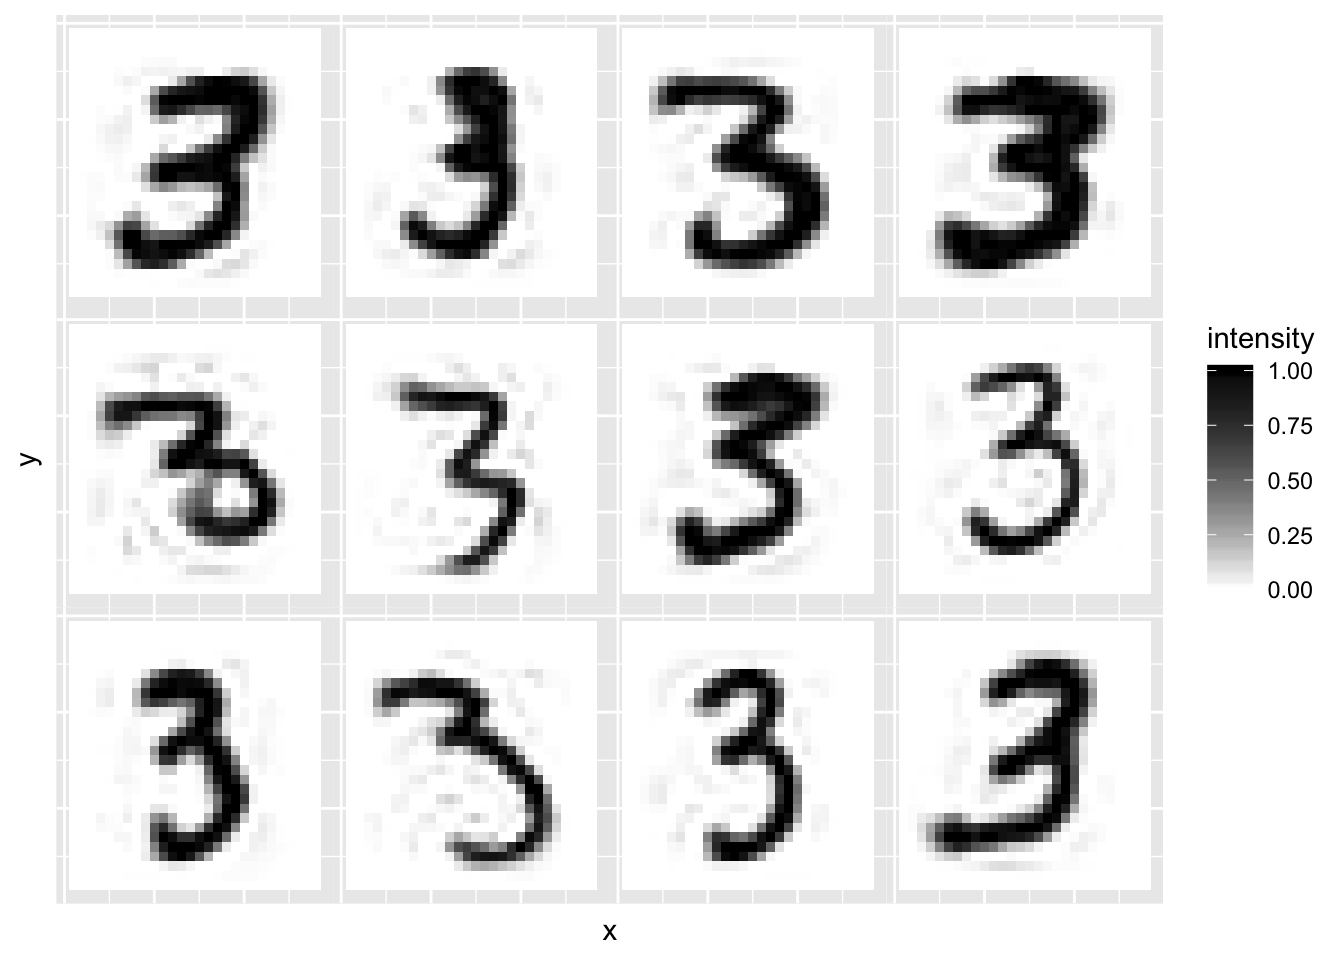
\includegraphics{04-pca_files/figure-latex/unnamed-chunk-42-1.pdf}

We can then finding images that differ according to these two PC scores. The first plot below is the 3 with the smallest PC1 score, and the second has the largest PC1 score. The third plot has the smallest PC2 score, and the fourth plot the largest PC2 score.
These four different 3s differ in more than just the first two principal components, but you can see the effect of the PC1 score is to slant the image forward or backward, whereas PC2 changes the thickness of the line.

\begin{Shaded}
\begin{Highlighting}[]
\NormalTok{image\_list }\OtherTok{\textless{}{-}} \FunctionTok{c}\NormalTok{(}\FunctionTok{which.min}\NormalTok{(mnist3.pca}\SpecialCharTok{$}\NormalTok{x[,}\DecValTok{1}\NormalTok{]), }
                \FunctionTok{which.max}\NormalTok{(mnist3.pca}\SpecialCharTok{$}\NormalTok{x[,}\DecValTok{1}\NormalTok{]),}
                \FunctionTok{which.min}\NormalTok{(mnist3.pca}\SpecialCharTok{$}\NormalTok{x[,}\DecValTok{2}\NormalTok{]), }
                \FunctionTok{which.max}\NormalTok{(mnist3.pca}\SpecialCharTok{$}\NormalTok{x[,}\DecValTok{2}\NormalTok{]))}
\FunctionTok{plot.mnist}\NormalTok{(mnist3[image\_list,]) }\CommentTok{\# plot the first 12 images}
\end{Highlighting}
\end{Shaded}

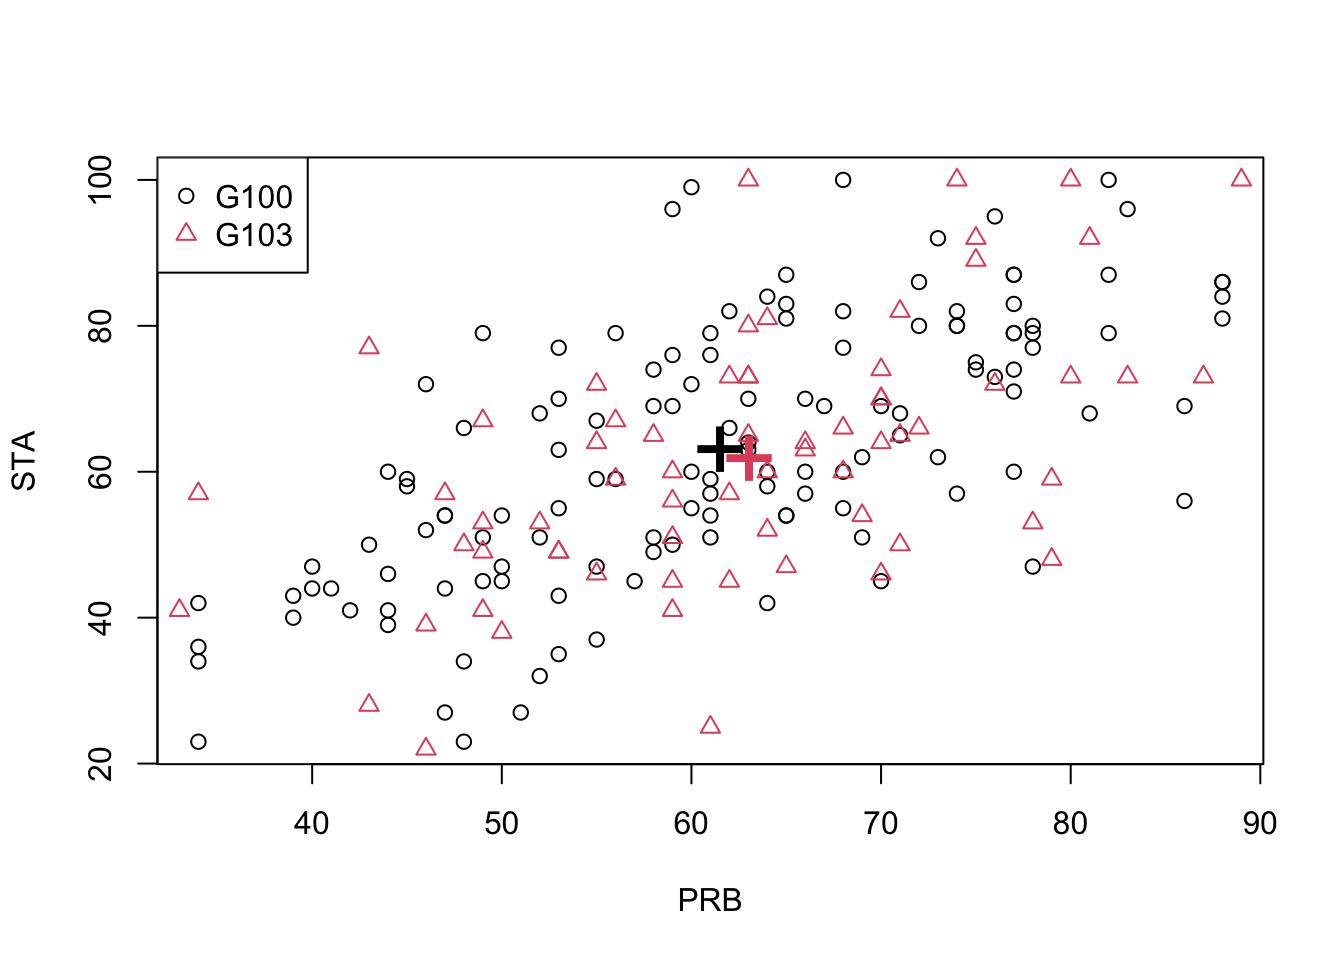
\includegraphics{04-pca_files/figure-latex/unnamed-chunk-43-1.pdf}

Finally, let's do PCA on a selection of the 60,000 images (not just the 3s). You can compute the SVD (which is what \texttt{prcomp} uses to do PCA) on a \(60,000 \times 784\) matrix, but it takes a long time on most computers, so here I've just computed the first two components on a random selection of 5,000 images using the option \texttt{rank=2} which significantly speeds up the computation time.

\begin{Shaded}
\begin{Highlighting}[]
\CommentTok{\# Note this is slow to compute!}
\NormalTok{image\_index }\OtherTok{\textless{}{-}} \FunctionTok{sample}\NormalTok{(}\DecValTok{1}\SpecialCharTok{:}\DecValTok{60000}\NormalTok{, }\AttributeTok{size=}\DecValTok{5000}\NormalTok{) }
\CommentTok{\# select a random sample of images}
\NormalTok{mnist.pca }\OtherTok{\textless{}{-}} \FunctionTok{prcomp}\NormalTok{(mnist}\SpecialCharTok{$}\NormalTok{train}\SpecialCharTok{$}\NormalTok{x[image\_index,], }\AttributeTok{rank=}\DecValTok{2}\NormalTok{)}
\NormalTok{Digit }\OtherTok{=} \FunctionTok{as.factor}\NormalTok{(mnist}\SpecialCharTok{$}\NormalTok{train}\SpecialCharTok{$}\NormalTok{y[image\_index])}
\FunctionTok{ggplot}\NormalTok{(}\FunctionTok{as.data.frame}\NormalTok{(mnist.pca}\SpecialCharTok{$}\NormalTok{x), }\FunctionTok{aes}\NormalTok{(}\AttributeTok{x=}\NormalTok{PC1, }\AttributeTok{y=}\NormalTok{PC2, }\AttributeTok{colour=}\NormalTok{Digit, }
                                       \AttributeTok{label=}\NormalTok{Digit))}\SpecialCharTok{+}
\FunctionTok{geom\_text}\NormalTok{(}\FunctionTok{aes}\NormalTok{(}\AttributeTok{label=}\NormalTok{Digit))}
\end{Highlighting}
\end{Shaded}

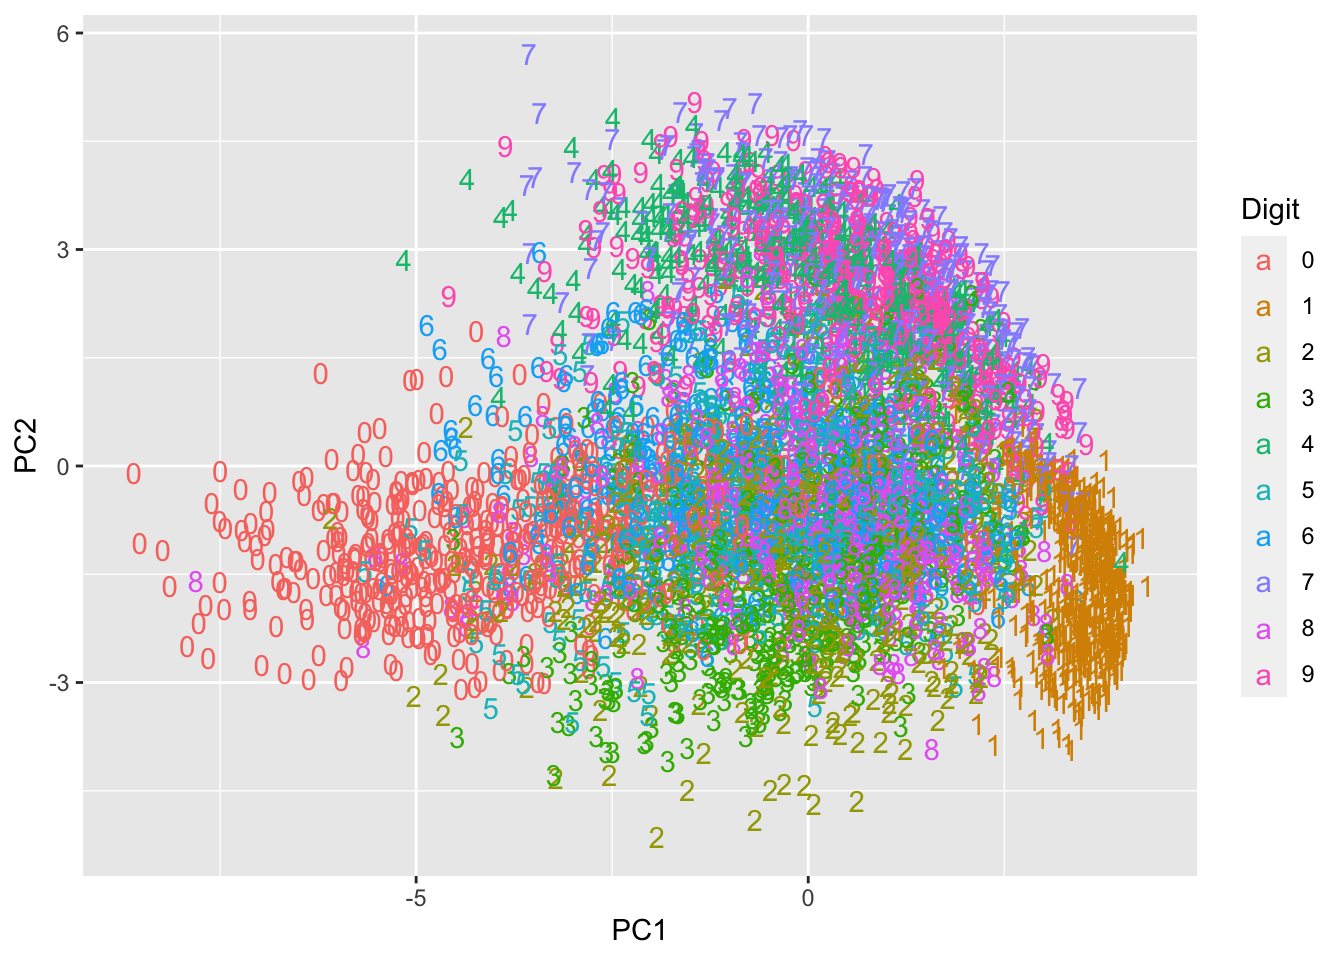
\includegraphics{04-pca_files/figure-latex/unnamed-chunk-44-1.pdf}

We can see from this scatter plot that the first two principal components do a surprisingly good job of separating and clustering the digits.

\section{Computer tasks}\label{pca-comptask}

\paragraph*{Exercise 1}\label{exercise-1}
\addcontentsline{toc}{paragraph}{Exercise 1}

Using the \texttt{iris} dataset, familiarize yourself with the \texttt{prcomp} command and its output.

Now, instead of using \texttt{prcomp} we will do the analysis ourselves using the \texttt{eigen} command.

\begin{itemize}
\tightlist
\item
  Start by computing the sample mean and sample variance of the dataset (use \(n-1\) as the denominator when you compute the sample variance to get the same answer as provided by \texttt{prcomp}).
\item
  Now compute the eigenvalues and eigenvectors of the covariance matrix using \texttt{eigen}. Check that these agree with those computed by \texttt{prcomp} (noting that \texttt{prcomp} returns the standard deviation which is the square root of the eigenvalues).
\item
  Now compute the principal component scores by multiplying \(\mathbf X\) by the matrix of eigenvectors \(\mathbf V\). Check your answer agrees with the scores provided by \texttt{prcomp}.
\end{itemize}

Now we will do the same thing again, but using the \texttt{svd} command.

\begin{itemize}
\item
  Compute the column centred data matrix \(\frac{1}{\sqrt{n-1}}\mathbf H\mathbf X\).
\item
  Compute the SVD of \(\frac{1}{\sqrt{n-1}}\mathbf H\mathbf X\) and \(\mathbf H\mathbf X\). How are the two sets of singular values related, and how do they relate to the eigenvalues computed previously.
  Are the singular vectors of \(\frac{1}{\sqrt{n-1}}\mathbf H\mathbf X\) and \(\mathbf H\mathbf X\) the same?
\item
  Compute the SVD scores by doing both \(\mathbf H\mathbf X\mathbf V\) and \(\mathbf U\boldsymbol{\Sigma}\), where
  \[\mathbf H\mathbf X= \mathbf U\boldsymbol{\Sigma}\mathbf V^\top\]
  is the SVD of \(\mathbf H\mathbf X\).
\end{itemize}

\paragraph*{Exercise 2}\label{exercise-2}
\addcontentsline{toc}{paragraph}{Exercise 2}

In this question we will look at the crabs data from the \texttt{MASS} R package.
We will focus on the 5 continuous variables, all measured in mm:

\begin{itemize}
\tightlist
\item
  FL = frontal lobe size
\item
  RW = rear width
\item
  CL = carapace length
\item
  CW = carapace width
\item
  BD = body depth.
\end{itemize}

The sample size is \(200\).

\begin{Shaded}
\begin{Highlighting}[]
\FunctionTok{library}\NormalTok{(MASS)}
\NormalTok{?crabs }\CommentTok{\# read the help page to find out about the dataset}
\NormalTok{X}\OtherTok{=}\NormalTok{crabs[,}\DecValTok{4}\SpecialCharTok{:}\DecValTok{8}\NormalTok{]     }
\CommentTok{\# construct data matrix X with columns FL, RW, CL, CW, BD}
\end{Highlighting}
\end{Shaded}

\begin{itemize}
\tightlist
\item
  Carry out PCA on the data in \(X\) using the correlation matrix, including obtaining a scree plot and plotting the PC scores.
\end{itemize}

Some questions:

\begin{itemize}
\item
  Do you have any suggestions for an interpretation for the 1st PC?
\item
  Are you able to come up with an interpretation for the 2nd PC?
\item
  Do you think an analysis based on the sample covariance matrix \({\bf S}\) or the
  correlation matrix \({\bf R}\) is preferable with this dataset? Does it make much difference which is used?
\item
  Without doing any computation, think about what you expect the sample mean and sample covariance matrix to be for the PC scores. Check this numerically.
\item
  Now check other properties of the PC scores listed in proposition \ref{prp:pca2}.
\item
  Try the following transformations of the data.

  \begin{itemize}
  \item
    adding a constant to the data
    \[\mathbf z= \mathbf x+\mathbf c,\]
  \item
    scaling the data:
    \[\mathbf z= \mathbf D\mathbf x\]
    for some diagonal matrix \(\mathbf D\)
  \item
    rotating the data:
    \[\mathbf z= \mathbf U\mathbf x\]
    for some \(p\times p\) orthogonal matrix \(\mathbf U\).
    You can generate a random orthogonal matrix using the following commands
  \end{itemize}
\end{itemize}

\begin{Shaded}
\begin{Highlighting}[]
\FunctionTok{library}\NormalTok{(pracma)}
\NormalTok{U }\OtherTok{\textless{}{-}} \FunctionTok{randortho}\NormalTok{(}\DecValTok{5}\NormalTok{)}
\end{Highlighting}
\end{Shaded}

Check the effect of each transformation on the principal components (the loadings/eigenvectors), the principal component scores, and the variance of the principal components (the eigenvalues).

\paragraph*{Exercise 3}\label{exercise-3}
\addcontentsline{toc}{paragraph}{Exercise 3}

Download the final Premier League table for the 2022-23 season from
\url{https://www.rotowire.com/soccer/league-table.php?season=2022}. There is a button to download the csv (comma separated variable) file in the bottom right hand corner.

\begin{itemize}
\item
  Load the data into R using the command \texttt{read.csv}. Note that you may need to manually delete the first row of the csv file before doing this. This can be done by clicking on the file name in the File tab in Rstudio, or by opening the file in any text editor or spreadsheet.
\item
  Repeat the analysis from section \ref{pca:football}. Does the meaning of the principal components change? Was the 2018-19 league season notably different to the 2019-20 season (which is the season analysed in the notes)?
\end{itemize}

\paragraph*{Exercise 4}\label{exercise-4}
\addcontentsline{toc}{paragraph}{Exercise 4}

The \texttt{decathlon2} data from the \texttt{factoextra} package contains
data on 27 different decathletes' performances during two different competitions. Let's start by extracting their performance in the 10 different decathlon events at the Olympics.

\begin{Shaded}
\begin{Highlighting}[]
\FunctionTok{library}\NormalTok{(}\StringTok{"factoextra"}\NormalTok{)}
\end{Highlighting}
\end{Shaded}

\begin{verbatim}
## Welcome! Want to learn more? See two factoextra-related books at https://goo.gl/ve3WBa
\end{verbatim}

\begin{Shaded}
\begin{Highlighting}[]
\FunctionTok{data}\NormalTok{(decathlon2)}
\NormalTok{X }\OtherTok{\textless{}{-}}\NormalTok{ decathlon2}\SpecialCharTok{|\textgreater{}}\NormalTok{ dplyr}\SpecialCharTok{::}\FunctionTok{filter}\NormalTok{(Competition}\SpecialCharTok{==}\StringTok{\textquotesingle{}OlympicG\textquotesingle{}}\NormalTok{) }\SpecialCharTok{|\textgreater{}}\NormalTok{ dplyr}\SpecialCharTok{::}\FunctionTok{select}\NormalTok{(}\SpecialCharTok{{-}}\NormalTok{Rank, }\SpecialCharTok{{-}}\NormalTok{Points,}\SpecialCharTok{{-}}\NormalTok{Competition)}
\end{Highlighting}
\end{Shaded}

Conduct PCA on these data, thinking about whether it is appropriate to use the correlation or covariance matrix. Give a scree plot, and determine how much information in the data is retained by the first two PCs.
Interpret the leading PCs.

Plot the first two scores for the different athlete performances, labelling each point. From these plots, comment on particular strengths/weaknesses in some performances.

\section{Exercises}\label{exercises-1}

\begin{enumerate}
\def\labelenumi{\arabic{enumi}.}
\tightlist
\item
  Consider the following data in \(\mathbb{R}^2\)
\end{enumerate}

\[\mathbf x_1 =\begin{pmatrix}1\\-1\end{pmatrix},\; \mathbf x_2 =\begin{pmatrix}-1\\1\end{pmatrix},
\;\mathbf x_3 =\begin{pmatrix}2\\2\end{pmatrix}\]

\begin{itemize}
\item
  What is the orthogonal projection of these points onto \[\mathbf u_1 = \begin{pmatrix}1\\0\end{pmatrix}\] and onto \[\mathbf u_2 =\frac{1}{\sqrt{5}}\begin{pmatrix}1\\2\end{pmatrix}?\]
\item
  Compute the sample variance matrix of the data points, and compute its spectral decomposition.
\item
  Which unit vector \(\mathbf u\) would maximize the variance of these projections?
\item
  What vector \(\mathbf u\) would minimize
  \[\sum_{i=1}^4 ||\mathbf x_i -\mathbf u\mathbf u^\top \mathbf x_i||^2_2?\]
  This is the sum of squared errors from a rank 1 approximation to the data.
\item
  Plot the data points and convince yourself that your answers make intuitive sense.
\end{itemize}

\begin{enumerate}
\def\labelenumi{\arabic{enumi}.}
\setcounter{enumi}{1}
\tightlist
\item
  Consider a population covariance matrix \(\boldsymbol{\Sigma}\) of the form
  \[\boldsymbol{\Sigma}=\gamma \mathbf I_p + \mathbf a\mathbf a^\top\]
  where \(\gamma>0\) is a scalar, \(\mathbf I_p\) is the \(p \times p\) identity matrix and \(\mathbf a\) is a vector of dimension \(p\).

  \begin{itemize}
  \tightlist
  \item
    Show that \(\mathbf a\) is an eigenvector of \(\boldsymbol{\Sigma}\).
  \item
    Show that if \(\mathbf b\) is any vector such that \(\mathbf a^\top \mathbf b=0\), then \(\mathbf b\) is also an eigenvector of \(\boldsymbol{\Sigma}\). What is the eigenvalue corresponding to \(\mathbf b\)?
  \item
    Obtain all the eigenvalues of \(\boldsymbol{\Sigma}\).
  \item
    Determine expressions for the proportion of variability `explained' by:
  \end{itemize}

  \begin{enumerate}
  \def\labelenumii{\roman{enumii}.}
  \tightlist
  \item
    the largest (population) principal component of \(\boldsymbol{\Sigma}\);
  \item
    the \(r\) largest (population) principal components of \(\boldsymbol{\Sigma}\), where \(1 < r \leq p\).
  \end{enumerate}
\item
  A covariance matrix has the following eigenvalues:
\end{enumerate}

\begin{verbatim}
##  [1] 4.22 2.38 1.88 1.11 0.91 0.82 0.58 0.44 0.35 0.19 0.05 0.04 0.04
\end{verbatim}

\begin{itemize}
\tightlist
\item
  Sketch a scree plot.
\item
  Determine the minimum number of principal components needed to explain 90\% of the total variation.
\item
  Determine the number of principal components whose eigenvalues are above average.
\end{itemize}

\begin{enumerate}
\def\labelenumi{\arabic{enumi}.}
\setcounter{enumi}{3}
\item
  Measurements are taken on \(p=3\) variables \(x_1\), \(x_2\) and \(x_3\), with sample correlation matrix
  \[
   \mathbf R= \begin{pmatrix} 1 & 0.5792 & 0.2414 \\ 0.5792 & 1 & 0.5816 \\ 0.2414 & 0.5816 & 1 \end{pmatrix}.
  \]
  The variable \(z_j\) is the standardised versions of \(x_j\), \(j=1,2,3\), i.e.~each \(z_j\) has sample mean \(0\) and variance \(1\).
  One observation has \(z_1 = z_2 = z_3 = 0\) and a second observation has \(z_1 = z_2 = z_3 =1\). Calculate the three
  principal component scores for
  each of these observations.
\item
  Try exam question 1 part (a) from the 2017-18 exam paper.
\end{enumerate}

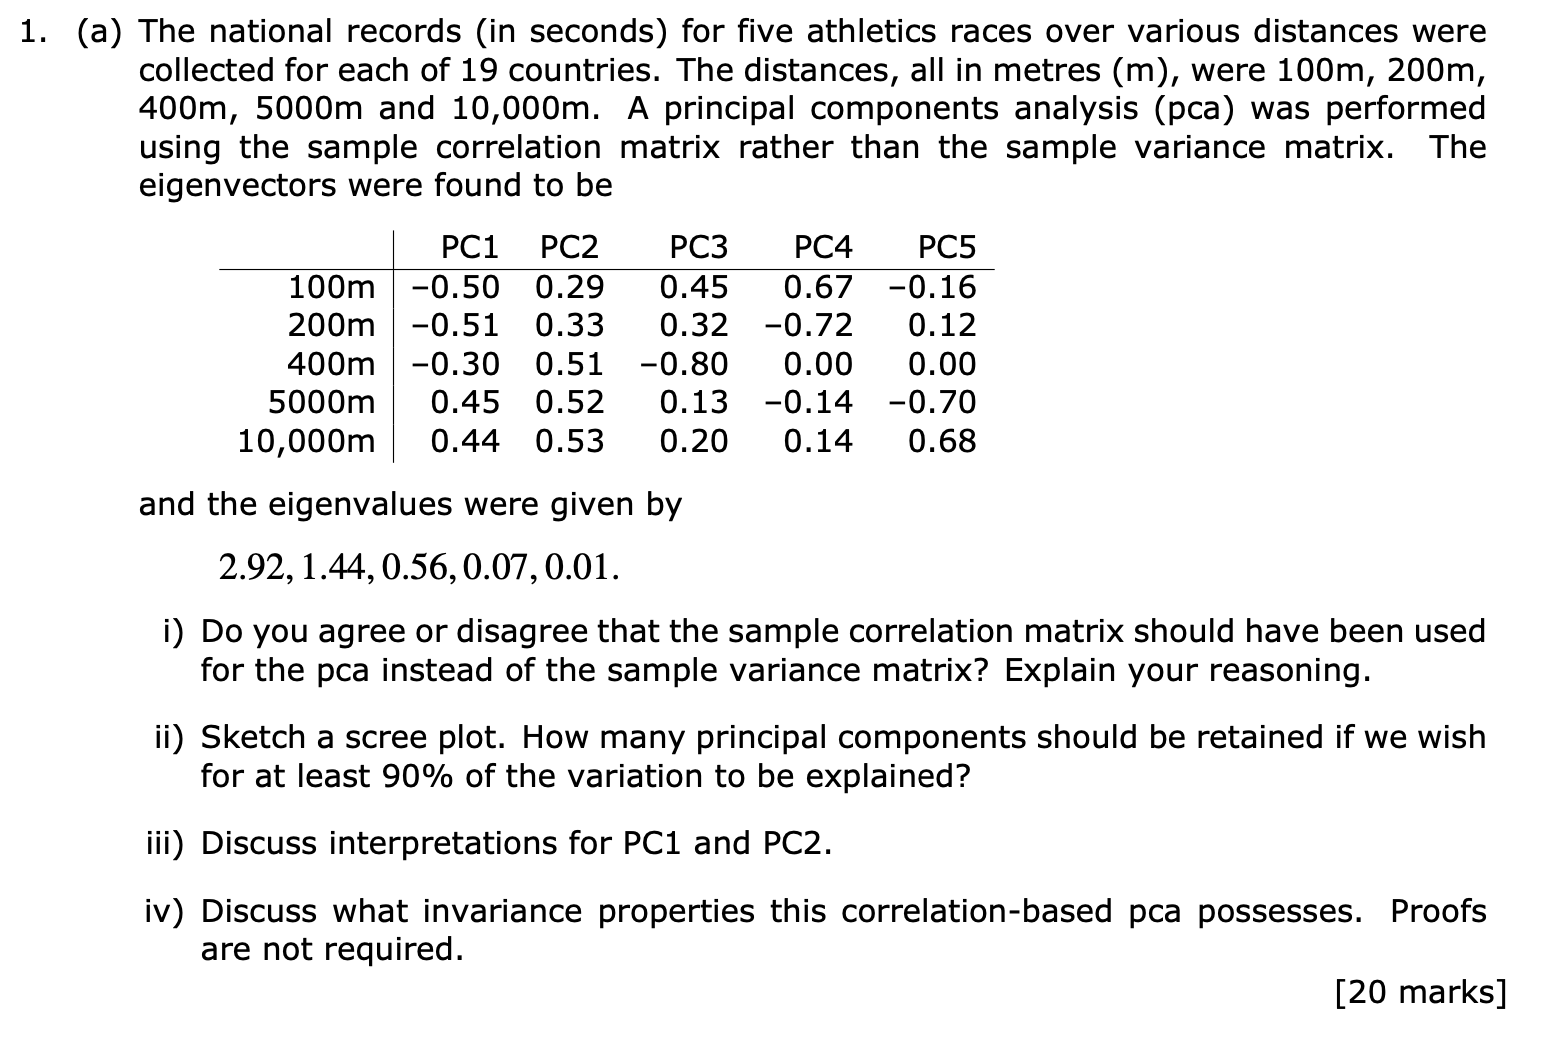
\includegraphics{figs/PCA_2017_18_Q1.png}

\begin{enumerate}
\def\labelenumi{\arabic{enumi}.}
\setcounter{enumi}{5}
\tightlist
\item
  Try this tricky question from the 2016 exam.
\end{enumerate}

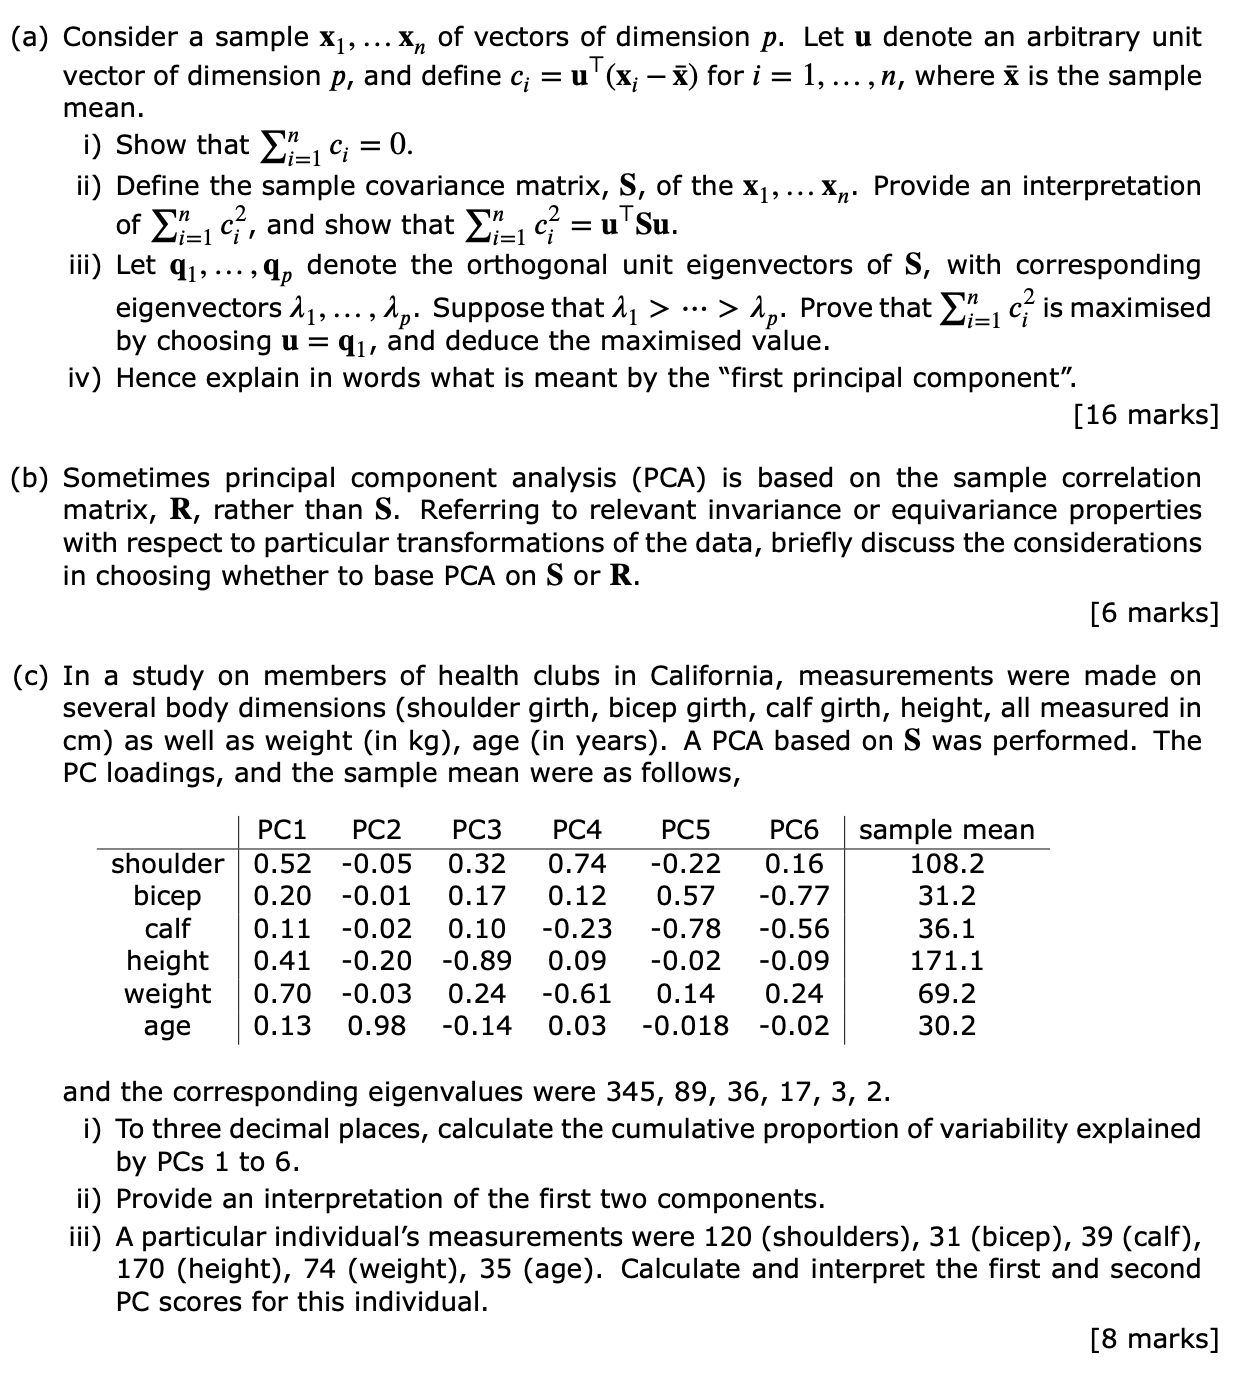
\includegraphics{PCA_Q4_2015_16.png}

\chapter{Canonical Correlation Analysis (CCA)}\label{cca}

The videos for this chapter are available at the following links

\begin{itemize}
\tightlist
\item
  \href{https://mediaspace.nottingham.ac.uk/media/CCA+Introduction/1_qhk7v35f}{5.1: Introduction to CCA}
\item
  \href{https://mediaspace.nottingham.ac.uk/media/CCAA+First+CC/1_yjm6kkxf}{5.1.1: The first pair of CC variables}
\item
  \href{https://mediaspace.nottingham.ac.uk/media/CCAA+Football+Example/1_r2v6924j}{5.1.2: Example: Premier league data}
\item
  \href{https://mediaspace.nottingham.ac.uk/media/CCAA+Full+Set/1_xmdoi9i6}{5.2: The full set of CC variables}
\item
  \href{https://mediaspace.nottingham.ac.uk/media/CCA\%3A\%20Properties/1_g24h27bj}{5.3: Properties of CCA}
\end{itemize}

Suppose we observe a random sample of \(n\) bivariate observations
\[
\mathbf z_1=(x_1,y_1)^\top , \ldots , \mathbf z_n=(x_n,y_n)^\top.
\]
If we are interested in exploring possible dependence between the \(x_i\)'s and \(y_i\)'s then among the first things we would do would be to obtain a scatterplot of the \(x_i\)'s against the \(y_i\)'s and calculate the correlation coefficient. Recall that the sample correlation coefficient is defined by
\begin{align}
r={\mathbb{C}\operatorname{or}}(x,y)&=\frac{S_{xy}}{\sqrt{S_{xx}}\sqrt{S_{yy}}}\\
&=\frac{\sum_{i=1}^n (x_i-\bar{x})(y_i-\bar{y})}{\left(\sum_{i=1}^n (x_i-\bar{x})^2  \right)^{1/2}  \left(\sum_{i=1}^n (y_i-\bar{y})^2 \right)^{1/2}}
\label{eq:scr}
\end{align}
where \(\bar{x}=n^{-1}\sum_{i=1}^n x_i\) and \(\bar{y}=n^{-1}\sum_{i=1}^n y_i\) are the sample means.

Recall that the sample correlation is a \textbf{scale-free measure} of the strength of the \textbf{linear dependence} between the \(x_i\)'s and the \(y_i\)'s.

In this chapter we investigate the multivariate analogue of this question. Instead of our bivariate observations being a pair of scalars, suppose instead that we are given two different random vectors \(\mathbf x\) and \(\mathbf y\). In otherwords, for each subject/case \(i\) we have observations
\(\{\mathbf x_i,\mathbf y_i\}_{i=1}^n.\)

Multivariate data structures can be understood better if we look at low-dimensional projections of the data. The question is, given a sample \(\{\mathbf x_i, \; \mathbf y_i\}_{i=1}^{n}\), what is a sensible way to assess and describe the strength of the linear dependence between the two vectors?

Canonical correlation analysis (CCA) gives an answer to this question in terms of the best low-dimensional linear projections of the \(\mathbf x\) and \(\mathbf y\) random variables. In a comparable way to PCA, `best' in CCA is defined in terms of maximizing correlations.
A key role is played by the singular value decomposition (SVD) introduced in Chapter \ref{linalg-decomp}.

\section{The first pair of canonical variables}\label{cca1}

\subsubsection*{Some notation}\label{some-notation}
\addcontentsline{toc}{subsubsection}{Some notation}

Assume we are given a random sample of vectors \(\mathbf x_i, \mathbf y_i\), and that we stack these into a vector \(\mathbf z_i\)
\[
\mathbf z_i=\left(\begin{array}{c}
\mathbf x_i\\
\mathbf y_i
\end{array}\right)=(\mathbf x_i^\top , \mathbf y_i^\top )^\top,\quad  i=1,\ldots, n,
\]
where
the \(\mathbf x_i\) are \(p \times 1\), the \(\mathbf y_i\) are \(q \times 1\) and, consequently, the \(\mathbf z_i\) are \((p+q)\times 1\). We are interested in determining the strength of linear association between the \(\mathbf x_i\) vectors and the \(\mathbf y_i\) vectors.
We formulate this task as an optimisation problem (cf.~PCA).

First, some notation:

\begin{itemize}
\item
  Let \(\bar{\mathbf x}\), \(\bar{\mathbf y}\), and \(\bar{\mathbf z}\) denote the sample mean vectors of the \(\mathbf x_i\), \(\mathbf y_i\) and \(\mathbf z_i\) respectively.
\item
  Let \(\mathbf S_{\mathbf z\mathbf z}\) denote the sample covariance matrix of the \(\mathbf z_i\), \(i=1,\ldots, n\). Then \(\mathbf S_{\mathbf z\mathbf z}\) can be written in block matrix form
  \[
  \mathbf S_{\mathbf z\mathbf z}=\left [\begin{array}{cc}
  \mathbf S_{\mathbf x\mathbf x} & \mathbf S_{\mathbf x\mathbf y}\\
  \mathbf S_{\mathbf y\mathbf x} & \mathbf S_{\mathbf y\mathbf y} \end{array} \right ],
  \]
  where \(\mathbf S_{\mathbf x\mathbf x}\) (\(p \times p\)) is the sample covariance matrix of the \(\mathbf x_i\), \(\mathbf S_{\mathbf y\mathbf y}\) (\(q \times q\)) is the sample covariance of the \(\mathbf y_i\), and the cross-covariance matrices are given by
  \[
  \stackrel{p \times q}{\mathbf S}_{\mathbf x\mathbf y}=n^{-1} \sum_{i=1}^n (\mathbf x_i -\bar{\mathbf x})(\mathbf y_i-\bar{\mathbf y})^\top
  \qquad \text{and} \qquad \stackrel{q \times p}{\mathbf S}_{\mathbf y\mathbf x}=\mathbf S_{\mathbf x\mathbf y}^\top.
  \]
\end{itemize}

\subsubsection*{Defining the optimization objective}\label{defining-the-optimization-objective}
\addcontentsline{toc}{subsubsection}{Defining the optimization objective}

We want to find the linear combination of the \(\mathbf x\)-variables and the linear combination of the \(\mathbf y\)-variables which is most highly correlated.

One version of the optimisation problem we want to solve is: find non-zero vectors \(\stackrel{p \times 1}{\mathbf a}\) and \(\stackrel{q \times 1}{\mathbf b}\) which maximise the correlation coefficient
\[
{\mathbb{C}\operatorname{or}}(\mathbf a^\top \mathbf x,\mathbf b^\top \mathbf y)=\frac{\mathbf a^\top \mathbf S_{\mathbf x\mathbf y}\mathbf b}{(\mathbf a^\top \mathbf S_{\mathbf x\mathbf x}\mathbf a)^{1/2}(\mathbf b^\top \mathbf S_{\mathbf y\mathbf y}\mathbf b)^{1/2}}.
\]
In other words:
\begin{align}
&\mbox{Maximise} \qquad\qquad \quad  {\mathbb{C}\operatorname{or}}(\mathbf a^\top \mathbf x,\mathbf b^\top \mathbf y),
\label{eq:opt26}\\
  &\mbox{for non-zero vectors}\quad  \mathbf a\;\; (p \times 1)\mbox{ and  } \mathbf b\;\; (q \times 1) \nonumber
\end{align}

where \({\mathbb{C}\operatorname{or}}(\cdot,\cdot)\) is defined in \eqref{eq:scr}.

Intuitively, this objective makes sense, because we want to find the linear combination of the \(\mathbf x\)-variables and the linear combination of the \(\mathbf y\)-variables which are most highly correlated.
However, note that for any \(\gamma>0\) and \(\delta>0\),
\begin{align}
  {\mathbb{C}\operatorname{or}}(\gamma\mathbf a^\top \mathbf x, \delta \mathbf b^\top \mathbf y)&= \frac{\gamma \delta}{\sqrt{\gamma^2 \delta^2}}{\mathbb{C}\operatorname{or}}(\mathbf a^\top \mathbf x,\mathbf b^\top \mathbf y)\\
  &={\mathbb{C}\operatorname{or}}(\mathbf a^\top \mathbf x,\mathbf b^\top \mathbf y).
  \label{eq:invar}
  \end{align}
\({\mathbb{C}\operatorname{or}}(\mathbf a^\top \mathbf x,\mathbf b^\top \mathbf y)\) is invariant to (i.e.~unchanged by) multiplication of \(\mathbf a\) and \(\mathbf b\) by positive scalars. Consequently there will be an infinite number of solutions to this optimisation problem, because if \(\mathbf a\) and \(\mathbf b\) are solutions, then so are \(\gamma \mathbf a\) and \(\delta \mathbf b\), for any \(\gamma>0\) and \(\delta>0\).

A more useful way to formulate this optimisation problem is

\begin{align}
&\mbox{Maximize }\qquad \mathbf a^\top \mathbf S_{\mathbf x\mathbf y}\mathbf b
\label{eq:opt27a}\\
  &\mbox{subject to } \qquad  \mathbf a^\top \mathbf S_{\mathbf x\mathbf x}\mathbf a=\mathbf b^\top \mathbf S_{\mathbf y\mathbf y}\mathbf b=1.\nonumber
\end{align}

Thankfully, there is a link between the solutions of the two optimization problems \eqref{eq:opt26} and \eqref{eq:opt27a}. Firstly, the invariance of \({\mathbb{C}\operatorname{or}}(\mathbf a^\top \mathbf x, \mathbf b^\top \mathbf y)\) means that if
\(\check{\mathbf a}\) and \(\check{\mathbf b}\) are a solution to problem \eqref{eq:opt27a}, then for any \(\gamma,\;\delta>0\), we have that \(\mathbf a=\gamma \check{\mathbf a}\) and \(\mathbf b=\delta \check{\mathbf b}\) are a solution to \eqref{eq:opt26}.

Conversely, we can convert any solution to optimization problem \eqref{eq:opt26} to be a solution to the problem \eqref{eq:opt27a}:

\begin{proposition}
\protect\hypertarget{prp:unnamed-chunk-1}{}\label{prp:unnamed-chunk-1}If \(\mathbf a\) and \(\mathbf b\) maximise \eqref{eq:opt26}, then
\[
\check{\mathbf a}=\frac{\mathbf a}{(\mathbf a^\top \mathbf S_{\mathbf x\mathbf x}{\mathbf a})^{1/2}} \qquad \text{and} \qquad
\check{\mathbf b}= \frac{{\mathbf b}}{({\mathbf b}^\top \mathbf S_{\mathbf y\mathbf y}{\mathbf b})^{1/2}}
\]
are a solution to the constrained maximization problem \eqref{eq:opt27a}.
\end{proposition}

\begin{proof}
Suppose \({\mathbf a}\) and \({\mathbf b}\) are solutions to optimization problem \eqref{eq:opt26}. Then invariance with respect to rescaling implies that \(\check{\mathbf a}={\mathbf a}/({\mathbf a}^\top \mathbf S_{\mathbf x\mathbf x} {\mathbf a})^{1/2}\) and \(\check{\mathbf b}= {\mathbf b}/({\mathbf b}^\top \mathbf S_{\mathbf y\mathbf y} {\mathbf b})^{1/2}\) also achieve the optima.
But \(\check{\mathbf a}\) and \(\check{\mathbf b}\) satisfy the constraints \(\mathbf a^\top \mathbf S_{\mathbf x\mathbf x}\mathbf a=\mathbf b^\top \mathbf S_{\mathbf y\mathbf y}\mathbf b=1\)
because
\[
\check{\mathbf a}^\top \mathbf S_{\mathbf x\mathbf x} \check{\mathbf a}=\frac{{\mathbf a}^\top \mathbf S_{\mathbf x\mathbf x}{\mathbf a}}{\left \{ \left ({\mathbf a}^\top \mathbf S_{\mathbf x\mathbf x}{\mathbf a}\right )^{1/2}\right \}^2}
=\frac{{\mathbf a}^\top \mathbf S_{\mathbf x\mathbf x}{\mathbf a}}{{\mathbf a}^\top \mathbf S_{\mathbf x\mathbf x}{\mathbf a}}=1
\]
and similarly for \(\check{\mathbf b}\).
So \(\check{\mathbf a}\) and \(\check{\mathbf b}\) maximises \eqref{eq:opt27a} subject to the constraints.
\end{proof}

\subsection{The first canonical components}\label{the-first-canonical-components}

As in the chapter on PCA, the optimal solution for CCA can be computed using the singular value decomposition. Before we describe the result, let's prove the following proposition from Chapter \ref{linalg-decomp}

\begin{proposition}
\protect\hypertarget{prp:svdmax2}{}\label{prp:svdmax2}For any matrix \(\mathbf Q\), we have
\[
\max_{\mathbf a, \mathbf b:\, \vert \vert \mathbf a\vert \vert=\vert \vert \mathbf b\vert \vert =1} \mathbf a^\top \mathbf Q\mathbf b=\sigma_1.
\]
with the maximum obtained at \(\mathbf a=\mathbf u_1\) and \(\mathbf b=\mathbf v_1\), the first left and right singular vectors of \(\mathbf Q\).
\end{proposition}

\begin{proof}
We'll use the method of Lagrange multipliers to prove this result. Consider the objective
\[\mathcal{L} = \mathbf a^\top \mathbf Q\mathbf b+\frac{\lambda_1}{2}(1-\mathbf a^\top\mathbf a)+\frac{\lambda_2}{2} (1-\mathbf b^\top \mathbf b).\]
The factor of 1/2 is there to simplify the maths once we differentiate.
Differentiating with respect to \(\mathbf a\) and \(\mathbf b\) and setting the derivative equal to zero gives
\begin{align}
{\boldsymbol 0}&= \mathbf Q\mathbf b-\lambda_1 \mathbf a\label{eq:ccaevp1}\\
{\boldsymbol 0}&= \mathbf Q^\top\mathbf a-\lambda_2 \mathbf b\label{eq:ccaevp2}
\end{align}
where for the second equation we've noted that \(\mathbf a^\top \mathbf Q\mathbf b= \mathbf b^\top \mathbf Q^\top \mathbf a\).
Left multiplying the first equation by \(\mathbf a^\top\) and the second by \(\mathbf b^\top\), and recalling that \(\mathbf a^\top \mathbf a=\mathbf b^\top\mathbf b=1\), shows that the two Lagrange multipliers are the same \(\lambda_1 = \lambda_2 =: \lambda\) say.

Substituting \(\mathbf a=\mathbf Q\mathbf b/\lambda\) into \eqref{eq:ccaevp2} gives
\[\mathbf Q^\top\mathbf Q\mathbf b= \lambda^2\mathbf b,\]
and so we can see that \(\mathbf b\) is an eigenvector of \(\mathbf Q^\top \mathbf Q\), and thus we must have \(\mathbf b= \mathbf v_i\) for some \(i\), i.e., \(\mathbf b\) is one of the right singular vectors of \(\mathbf Q\). Similarly, substituting \(\mathbf b= \mathbf Q^\top \mathbf a/\lambda\) into \eqref{eq:ccaevp1} gives
\[\mathbf Q\mathbf Q^\top \mathbf a= \lambda^2\mathbf a.\]
So \(\mathbf a=\mathbf u_j\) for some \(j\), i.e., \(\mathbf a\) is one of the left singular vectors of \(\mathbf Q\).

Finally, consider the original objective with \(\mathbf a=\mathbf u_j\) and \(\mathbf b=\mathbf v_i\):
\[\mathbf u_j^\top\mathbf Q\mathbf v_i = \sigma_i\mathbf u_j^\top \mathbf u_i = \begin{cases} \sigma_i &\mbox{ if } i = j\\
0 &\mbox{ otherwise.}
\end{cases}
\]
Hence we maximize the objective by taking \(\mathbf a=\mathbf u_1\) and \(\mathbf b=\mathbf v_1\), and then we find
\[\max_{\mathbf a, \mathbf b:\, \vert \vert \mathbf a\vert \vert=\vert \vert \mathbf b\vert \vert =1} \mathbf a^\top \mathbf Q\mathbf b=\sigma_1.\]
\end{proof}

\subsubsection*{Main result}\label{main-result}
\addcontentsline{toc}{subsubsection}{Main result}

We're now in a position to describe the main result giving the first pair of canonical variables

\begin{proposition}
\protect\hypertarget{prp:unnamed-chunk-2}{}\label{prp:unnamed-chunk-2}Assume that \(\mathbf S_{\mathbf x\mathbf x}\) and \(\mathbf S_{\mathbf y\mathbf y}\) are both non-singular, and consider the singular value decomposition of the matrix \(\mathbf Q:=\mathbf S_{\mathbf x\mathbf x}^{-1/2} \mathbf S_{\mathbf x\mathbf y}\mathbf S_{\mathbf y\mathbf y}^{-1/2}\)
\begin{equation}
\mathbf Q= {\mathbf U}{\pmb \Sigma} {\mathbf V}^\top = \sum_{j=1}^t \sigma_j {\mathbf u}_j {\mathbf v}_j^\top,
\label{eq:svdcca}
\end{equation}
where \(t=\operatorname{rank}(\mathbf Q)\) and \(\sigma_1 \geq \cdots \geq \sigma_t >0\).

Then the solution to the constrained optimization problem \eqref{eq:opt27a} is \[\mathbf a=\mathbf S_{\mathbf x\mathbf x}^{-1/2}{\mathbf u}_1\quad \mbox{and}\quad \mathbf b=\mathbf S_{\mathbf y\mathbf y}^{-1/2}{\mathbf v}_1.\]

The maximum value of the correlation coefficient is given by the largest singular value \(\sigma_1\):
\[\max_{\mathbf a, \mathbf b} {\mathbb{C}\operatorname{or}}(\mathbf a^\top\mathbf x, \mathbf b^\top\mathbf y)=\sigma_1.\]
\end{proposition}

\begin{proof}
If we let
\[
\tilde{\mathbf a}=\mathbf S_{\mathbf x\mathbf x}^{1/2} \mathbf a\qquad \text{and} \qquad \tilde{\mathbf b}=\mathbf S_{\mathbf y\mathbf y}^{1/2}\mathbf b,
\]
we may write the constraints \(\mathbf a^\top \mathbf S_{\mathbf x\mathbf x}\mathbf a=\mathbf b^\top \mathbf S_{\mathbf y\mathbf y}\mathbf b=1\) as
\[
\tilde{\mathbf a}^\top \tilde{\mathbf a}=1 \qquad \text{and} \qquad \tilde{\mathbf b}^\top \tilde{\mathbf b}=1.
\]

Because \(\mathbf S_{\mathbf x\mathbf x}\) and \(\mathbf S_{\mathbf y\mathbf y}\) are non-singular, \(\mathbf S_{\mathbf x\mathbf x}^{1/2}\) and \(\mathbf S_{\mathbf y\mathbf y}^{1/2}\) must also be non-singular, and so we can compute
\(\mathbf S_{\mathbf x\mathbf x}^{-1/2}\) and \(\mathbf S_{\mathbf y\mathbf y}^{-1/2}\), using the matrix square roots defined in Section \ref{matrixroots}.

If we write
\[
\mathbf a=\mathbf S_{\mathbf x\mathbf x}^{-1/2}\tilde{\mathbf a} \qquad \text{and} \qquad \mathbf b=\mathbf S_{\mathbf y\mathbf y}^{-1/2} \tilde{\mathbf b},
\]
then the optimisation problem \eqref{eq:opt27a} becomes
\[
\max_{\tilde{\mathbf a}, \tilde{\mathbf b}}
\tilde{\mathbf a}^\top \mathbf S_{\mathbf x\mathbf x}^{-1/2}\mathbf S_{\mathbf x\mathbf y}\mathbf S_{\mathbf y\mathbf y}^{-1/2} \tilde{\mathbf b}
\]
subject to
\[
\vert \vert \tilde{\mathbf a} \vert \vert =1 \qquad \text{and} \qquad \vert \vert \tilde{\mathbf b}\vert \vert=1.
\]

Then by Proposition \ref{prp:svdmax2} we can see that
\[\tilde{\mathbf a} = \mathbf u_1 \quad \mbox{and}\quad\tilde{\mathbf b} = \mathbf v_1\]
and the result follows.
\end{proof}

We will label the solution found as
\[\mathbf a_1 := \mathbf S_{xx}^{-\frac{1}{2}}\mathbf u_1\quad \mbox{ and }\quad\mathbf b_1 := \mathbf S_{yy}^{-\frac{1}{2}}\mathbf v_1\]
to stress that \(\mathbf a_1\) and \(\mathbf b_1\) are the \textbf{first} pair of \textbf{canonical correlation (CC) vectors}. The variables \(\eta_1=\mathbf a_1^\top (\mathbf x-\bar{\mathbf x})\) and \(\psi_1=\mathbf b_1^\top (\mathbf y-\bar{\mathbf y})\) are called the first pair of \textbf{canonical correlation variables}, and \(\sigma_1={\mathbb{C}\operatorname{or}}(\eta_1, \psi_1)\) is the \textbf{first canonical correlation}.

\subsection{Example: Premier league football}\label{premcca}

Lets again return to the Premier League from the previous chapter.

\begin{Shaded}
\begin{Highlighting}[]
\FunctionTok{library}\NormalTok{(dplyr)}
\NormalTok{prem1920 }\OtherTok{\textless{}{-}} \FunctionTok{read.csv}\NormalTok{(}\StringTok{\textquotesingle{}data/2019\_2020EPL.csv\textquotesingle{}}\NormalTok{) }
\CommentTok{\# the data can be downloaded from }
\CommentTok{\# https://www.rotowire.com/soccer/league{-}table.php}
\NormalTok{table }\OtherTok{\textless{}{-}}\NormalTok{ prem1920 }\SpecialCharTok{\%\textgreater{}\%}\NormalTok{ dplyr}\SpecialCharTok{::}\FunctionTok{select}\NormalTok{(Team, W, D, L, G, GA, GD) }
\NormalTok{knitr}\SpecialCharTok{::}\FunctionTok{kable}\NormalTok{(}\FunctionTok{head}\NormalTok{(table,}\DecValTok{5}\NormalTok{), }\AttributeTok{booktabs =} \ConstantTok{TRUE}\NormalTok{, }\AttributeTok{escape=}\ConstantTok{FALSE}\NormalTok{)}
\end{Highlighting}
\end{Shaded}

\begin{tabular}{lrrrrrr}
\toprule
Team & W & D & L & G & GA & GD\\
\midrule
Liverpool & 32 & 3 & 3 & 85 & 33 & 52\\
Manchester City & 26 & 3 & 9 & 102 & 35 & 67\\
Manchester United & 18 & 12 & 8 & 66 & 36 & 30\\
Chelsea & 20 & 6 & 12 & 69 & 54 & 15\\
Leicester City & 18 & 8 & 12 & 67 & 41 & 26\\
\bottomrule
\end{tabular}

We shall treat \(W\) and \(D\), the number of wins and draws, as the \(\mathbf x\)-variables. The number of goals for and against, \(G\) and \(GA\), will be treated as the \(\mathbf y\)-variables. The number of losses and the goal difference, \(L\) and \(GD\), are omitted as they provide no additional information when we know \(W\) and \(D\).

We shall consider the questions

\begin{itemize}
\tightlist
\item
  how strongly associated are the match outcome variables, \(W\) and \(D\), with the goals for and against variables, \(G\) and \(GA\)?
\item
  what linear combination of \(W\) and \(D\), and of \(G\) and \(GA\) are most strongly correlated?
\end{itemize}

Firstly, we need to compute the three covariance matrices needed for CCA. These are easily computed in R:

\begin{Shaded}
\begin{Highlighting}[]
\NormalTok{X }\OtherTok{\textless{}{-}}\NormalTok{ table[,}\FunctionTok{c}\NormalTok{(}\StringTok{\textquotesingle{}W\textquotesingle{}}\NormalTok{,}\StringTok{\textquotesingle{}D\textquotesingle{}}\NormalTok{)] }\CommentTok{\# W and D}
\NormalTok{Y }\OtherTok{\textless{}{-}}\NormalTok{ table[,}\FunctionTok{c}\NormalTok{(}\StringTok{\textquotesingle{}G\textquotesingle{}}\NormalTok{,}\StringTok{\textquotesingle{}GA\textquotesingle{}}\NormalTok{)] }\CommentTok{\# G and GA}
\NormalTok{S\_xx }\OtherTok{\textless{}{-}} \FunctionTok{cov}\NormalTok{(X)}
\NormalTok{S\_yy }\OtherTok{\textless{}{-}} \FunctionTok{cov}\NormalTok{(Y)}
\NormalTok{S\_xy }\OtherTok{\textless{}{-}} \FunctionTok{cov}\NormalTok{(X,Y)}
\end{Highlighting}
\end{Shaded}

giving

\[\mathbf S_{xx} =\begin{pmatrix}40.4&-9.66 \\-9.66&10.7 \\\end{pmatrix}, \quad \mathbf S_{yy} =\begin{pmatrix}354&-155 \\-155&141 \\\end{pmatrix}, \\
\quad \mathbf S_{xy}=\mathbf S_{yx}^\top =\begin{pmatrix}108&-60 \\-28.9&-2.36 \\\end{pmatrix}.\]

We now want to calculate the matrix \(\mathbf Q\) in \eqref{eq:svdcca} and then find its singular valued decomposition. We first need to find \(\mathbf S_{\mathbf x\mathbf x}^{-1/2}\) and \(\mathbf S_{\mathbf y\mathbf y}^{-1/2}\). Using R to do the computations we obtain the spectral decompositions

\begin{Shaded}
\begin{Highlighting}[]
\NormalTok{eigen\_xx }\OtherTok{\textless{}{-}} \FunctionTok{eigen}\NormalTok{(S\_xx)}
\NormalTok{Vx }\OtherTok{\textless{}{-}}\NormalTok{ eigen\_xx}\SpecialCharTok{$}\NormalTok{vectors}
\NormalTok{S\_xx\_invsqrt }\OtherTok{\textless{}{-}}\NormalTok{ Vx }\SpecialCharTok{\%*\%} \FunctionTok{diag}\NormalTok{(}\DecValTok{1}\SpecialCharTok{/}\FunctionTok{sqrt}\NormalTok{(eigen\_xx}\SpecialCharTok{$}\NormalTok{values)) }\SpecialCharTok{\%*\%} \FunctionTok{t}\NormalTok{(Vx)}
\CommentTok{\# check S\_xx \%*\% S\_xx\_invsqrt \%*\% S\_xx\_invsqrt }
\CommentTok{\# is the identity matrix}
\end{Highlighting}
\end{Shaded}

\[\mathbf S_{xx} =\mathbf Q\boldsymbol \Lambda\mathbf Q^\top=\begin{pmatrix}-0.959&-0.285 \\0.285&-0.959 \\\end{pmatrix} \begin{pmatrix}43.2&0 \\0&7.82 \\\end{pmatrix} \begin{pmatrix}-0.959&0.285 \\-0.285&-0.959 \\\end{pmatrix}\]

and so

\begin{align*}
\mathbf S_{\mathbf x\mathbf x}^{-1/2} &= \mathbf Q\boldsymbol \Lambda^{-\frac{1}{2}}\mathbf Q^\top \\
&=\begin{pmatrix}-0.959&-0.285 \\0.285&-0.959 \\\end{pmatrix} \begin{pmatrix}0.152&0 \\0&0.357 \\\end{pmatrix} \begin{pmatrix}-0.959&0.285 \\-0.285&-0.959 \\\end{pmatrix}\\
&= \begin{pmatrix}0.169&0.0561 \\0.0561&0.341 \\\end{pmatrix}.
\end{align*}

Similarly, we find

\begin{Shaded}
\begin{Highlighting}[]
\NormalTok{eigen\_yy }\OtherTok{\textless{}{-}} \FunctionTok{eigen}\NormalTok{(S\_yy)}
\NormalTok{Vy }\OtherTok{\textless{}{-}}\NormalTok{ eigen\_yy}\SpecialCharTok{$}\NormalTok{vectors}
\NormalTok{S\_yy\_invsqrt }\OtherTok{\textless{}{-}}\NormalTok{ Vy }\SpecialCharTok{\%*\%} \FunctionTok{diag}\NormalTok{(}\DecValTok{1}\SpecialCharTok{/}\FunctionTok{sqrt}\NormalTok{(eigen\_yy}\SpecialCharTok{$}\NormalTok{values)) }\SpecialCharTok{\%*\%} \FunctionTok{t}\NormalTok{(Vy)}
\end{Highlighting}
\end{Shaded}

\begin{align*}
\mathbf S_{\mathbf y\mathbf y}^{-1/2}= \begin{pmatrix}0.0657&0.0337 \\0.0337&0.112 \\\end{pmatrix}.
\end{align*}

Consequently,
\begin{align*}
\mathbf Q&=\mathbf S_{\mathbf x\mathbf x}^{-1/2}\mathbf S_{\mathbf x\mathbf y}\mathbf S_{\mathbf y\mathbf y}^{-1/2}\\
&=\begin{pmatrix}0.169&0.0561 \\0.0561&0.341 \\\end{pmatrix} \begin{pmatrix}108&-60 \\-28.9&-2.36 \\\end{pmatrix}\begin{pmatrix}0.0657&0.0337 \\0.0337&0.112 \\\end{pmatrix}\\
&=\begin{pmatrix}0.747&-0.588 \\-0.39&-0.595 \\\end{pmatrix}.
\end{align*}

The SVD of \(\mathbf Q\) is given by
\begin{align}
\mathbf Q&=\mathbf U{\pmb \Sigma} \mathbf V^\top \nonumber \\
&=\begin{pmatrix}-0.99&-0.143 \\-0.143&0.99 \\\end{pmatrix} \begin{pmatrix}0.955&0 \\0&0.705 \\\end{pmatrix}\begin{pmatrix}-0.715&-0.699 \\0.699&-0.715 \\\end{pmatrix}^\top
\label{eq:SVDanalysis}
\end{align}

So the 1st CC coefficient is \(0.955\), which is close to its maximum value of \(1\). The 1st CC weight vectors are
given by

\begin{Shaded}
\begin{Highlighting}[]
\NormalTok{a1 }\OtherTok{=}\NormalTok{ S\_xx\_invsqrt}\SpecialCharTok{\%*\%}\NormalTok{ Q\_svd}\SpecialCharTok{$}\NormalTok{u[,}\DecValTok{1}\NormalTok{]}
\NormalTok{b1 }\OtherTok{=}\NormalTok{ S\_yy\_invsqrt}\SpecialCharTok{\%*\%}\NormalTok{ Q\_svd}\SpecialCharTok{$}\NormalTok{v[,}\DecValTok{1}\NormalTok{]}
\end{Highlighting}
\end{Shaded}

\begin{align*}
\mathbf a_1&=\mathbf S_{\mathbf x\mathbf x}^{-1/2}\mathbf u_1\\
&=\begin{pmatrix}0.169&0.0561 \\0.0561&0.341 \\\end{pmatrix}\begin{pmatrix}-0.99 \\-0.143 \\\end{pmatrix}\\
&=\begin{pmatrix}-0.175 \\-0.104 \\\end{pmatrix}\\
\mathbf b_1 &=\mathbf S_{\mathbf y\mathbf y}^{-1/2}\mathbf v_1\\
&= \begin{pmatrix}-0.0234 \\0.0541 \\\end{pmatrix}
\end{align*}

This leads to the first pair of CC variables, obtained using these CC vectors/weights:
\[
\eta_1 =-0.175 (W-\bar{W}) +-0.104(D -\bar{D})
\]
and
\[
 \psi_1 = -0.0234(G-\bar{G}) +0.0541(GA-\bar{GA}).
\]

We can see that \(\psi_1\) is measuring something similar to goal difference \(G-GA\), as usually defined, but it gives higher weight to goals conceded than goals scored (\(0.0541\) versus \(0.0234\)).

\(\eta_1\) is measuring something similar to number of points \(3W+D\), as usually defined, but the ratio of points for a win to points for a draw is lower, at around 2:1, as opposed to the usual ratio 3:1.

The full list of the first canonical correlation variables is thus

\begin{Shaded}
\begin{Highlighting}[]
\NormalTok{Xcent }\OtherTok{\textless{}{-}} \FunctionTok{sweep}\NormalTok{(X,}\DecValTok{2}\NormalTok{, }\FunctionTok{colMeans}\NormalTok{(X)) }\CommentTok{\# column centre the matrix}
\NormalTok{Ycent }\OtherTok{\textless{}{-}} \FunctionTok{sweep}\NormalTok{(Y,}\DecValTok{2}\NormalTok{, }\FunctionTok{colMeans}\NormalTok{(Y)) }\CommentTok{\# column centre the matrix}
\NormalTok{eta }\OtherTok{=} \FunctionTok{as.matrix}\NormalTok{(Xcent)}\SpecialCharTok{\%*\%}\NormalTok{a1}
\NormalTok{psi }\OtherTok{=} \FunctionTok{as.matrix}\NormalTok{(Ycent)}\SpecialCharTok{\%*\%}\NormalTok{b1}
\end{Highlighting}
\end{Shaded}

\begin{tabular}{lrr}
\toprule
Team & eta & psi\\
\midrule
Liverpool & -2.4340723 & -1.7921117\\
Manchester City & -1.3838590 & -2.0820965\\
Manchester United & -0.9221199 & -1.1846733\\
Chelsea & -0.6464941 & -0.2807761\\
Leicester City & -0.5049886 & -0.9374949\\
\bottomrule
\end{tabular}

A scatter plot of the two canonical correlation variables shows the strong correlation between them.

\begin{Shaded}
\begin{Highlighting}[]
\NormalTok{cca.out }\OtherTok{\textless{}{-}} \FunctionTok{data.frame}\NormalTok{(}\AttributeTok{Team=}\NormalTok{table}\SpecialCharTok{$}\NormalTok{Team, }\AttributeTok{eta=}\NormalTok{eta, }\AttributeTok{psi=}\NormalTok{psi)}
\FunctionTok{library}\NormalTok{(ggplot2)}
\FunctionTok{ggplot}\NormalTok{(cca.out, }\FunctionTok{aes}\NormalTok{(}\AttributeTok{x=}\NormalTok{ eta, }\AttributeTok{y=}\NormalTok{ psi, }\AttributeTok{label=}\NormalTok{Team))}\SpecialCharTok{+}   \FunctionTok{geom\_point}\NormalTok{() }\SpecialCharTok{+}
\FunctionTok{geom\_text}\NormalTok{(}\FunctionTok{aes}\NormalTok{(}\AttributeTok{label=}\NormalTok{Team),}\AttributeTok{hjust=}\DecValTok{0}\NormalTok{, }\AttributeTok{vjust=}\DecValTok{0}\NormalTok{, }\AttributeTok{size=}\DecValTok{4}\NormalTok{)}
\end{Highlighting}
\end{Shaded}

\includegraphics{05-cca_files/figure-latex/unnamed-chunk-14-1.pdf}

We can also do this with the \texttt{CCA} package in R. The command \texttt{matcor(X,Y)} gives the correlation matrices, and the command \texttt{cc} performs CCA. See if you can find the outputs computed above in the output of the \texttt{cc} command.

\begin{Shaded}
\begin{Highlighting}[]
\FunctionTok{library}\NormalTok{(CCA)}
\NormalTok{prem.cca }\OtherTok{\textless{}{-}} \FunctionTok{cc}\NormalTok{(X,Y)}
\NormalTok{prem.cca}\SpecialCharTok{$}\NormalTok{cor }\CommentTok{\# the canonical correlations}
\end{Highlighting}
\end{Shaded}

\begin{verbatim}
## [1] 0.9550749 0.7054825
\end{verbatim}

\begin{Shaded}
\begin{Highlighting}[]
\NormalTok{prem.cca}\SpecialCharTok{$}\NormalTok{xcoef }\CommentTok{\# the canonical correlation vectors for X}
\end{Highlighting}
\end{Shaded}

\begin{verbatim}
##         [,1]      [,2]
## W -0.1750356 0.0313256
## D -0.1042828 0.3293057
\end{verbatim}

\begin{Shaded}
\begin{Highlighting}[]
\NormalTok{prem.cca}\SpecialCharTok{$}\NormalTok{ycoef  }\CommentTok{\# the canonical correlation vectors for Y}
\end{Highlighting}
\end{Shaded}

\begin{verbatim}
##           [,1]        [,2]
## G  -0.02342507 -0.07003113
## GA  0.05412069 -0.10372100
\end{verbatim}

\begin{Shaded}
\begin{Highlighting}[]
\FunctionTok{head}\NormalTok{(prem.cca}\SpecialCharTok{$}\NormalTok{scores}\SpecialCharTok{$}\NormalTok{xscores) }\CommentTok{\# the canonical correlation variables }
\end{Highlighting}
\end{Shaded}

\begin{verbatim}
##            [,1]       [,2]
## [1,] -2.4340723 -1.4903651
## [2,] -1.3838590 -1.6783187
## [3,] -0.9221199  1.0348282
## [4,] -0.6464941 -0.8783550
## [5,] -0.5049886 -0.2823947
## [6,] -0.4677660  0.6428713
\end{verbatim}

\begin{Shaded}
\begin{Highlighting}[]
\FunctionTok{head}\NormalTok{(prem.cca}\SpecialCharTok{$}\NormalTok{scores}\SpecialCharTok{$}\NormalTok{yscores) }\CommentTok{\# the canonical correlation variables }
\end{Highlighting}
\end{Shaded}

\begin{verbatim}
##            [,1]        [,2]
## [1,] -1.7921117 -0.39245373
## [2,] -2.0820965 -1.79042487
## [3,] -1.1846733  0.62697465
## [4,] -0.2807761 -1.45009678
## [5,] -0.9374949  0.03833851
## [6,] -0.4722204 -0.16380075
\end{verbatim}

\begin{Shaded}
\begin{Highlighting}[]
\CommentTok{\#prem.cca}
\CommentTok{\#plt.cc(prem.cca, var.label = TRUE, ind.names = table$Team)}
\end{Highlighting}
\end{Shaded}

\section{The full set of canonical correlations}\label{the-full-set-of-canonical-correlations}

Let us first recap what we did in the previous section: we found a linear combination of the \(\mathbf x\)-variables and a linear combination of the \(\mathbf y\)-variables which
maximised the correlation, and expressed the answer in terms of quantities which arise in the SVD of \(\mathbf Q\), where
\[
\mathbf Q\equiv \mathbf S_{\mathbf x\mathbf x}^{-1/2} \mathbf S_{\mathbf x\mathbf y}\mathbf S_{\mathbf y\mathbf y}^{-1/2}=\mathbf U{\pmb \Sigma} \mathbf V^\top=\sum_{j=1}^t \sigma_j \mathbf u_j \mathbf v_j^\top.
\]

We found the maximum value of the correlation \({\mathbb{C}\operatorname{or}}(\mathbf a^\top\mathbf x, \mathbf b^\top\mathbf y)\) to be \(\sigma_1\), achieved using the linear combinations \(\eta_1=\mathbf a_1^\top \mathbf x\) and \(\psi_1=\mathbf b_1^\top \mathbf y\) with

\[\mathbf a_1=\mathbf S_{\mathbf x\mathbf x}^{-1/2}\mathbf u_1 \quad\mbox{ and } \mathbf b_1=\mathbf S_{\mathbf y\mathbf y}^{-1/2}\mathbf v_1.\]

We now repeat this process to find the next most important linear combination, subject to being uncorrelated with the first linear combination, as we did with PCA. For \(\mathbf a^\top \mathbf x\) to be uncorrelated with \(\eta_1 = \mathbf a_1^\top \mathbf x\) we require
\[0 = {\mathbb{C}\operatorname{ov}}(\mathbf a_1^\top \mathbf x, \mathbf a^\top \mathbf x) = \mathbf a_1^\top \mathbf S_{xx}\mathbf a,\]
and similarly we require the condition \(\mathbf b_1^\top \mathbf S_{yy} \mathbf b=0\) for \(\mathbf b\).

Thus, to obtain the second canonical correlation coefficient, plus the associated sets of canonical correlation vectors and variables, we need to solve the following optimisation problem:
\begin{equation}
\max_{\mathbf a,\, \mathbf b} \mathbf a^\top \mathbf S_{\mathbf x\mathbf y}\mathbf b
\label{eq:cc2}
\end{equation}
subject to the constraints
\begin{equation}
\mathbf a^\top \mathbf S_{\mathbf x\mathbf x}\mathbf a= \mathbf b^\top \mathbf S_{\mathbf y\mathbf y}\mathbf b=1,
\label{eq:conny21}
\end{equation}
\begin{equation}
\mathbf a_1^\top \mathbf S_{\mathbf x\mathbf x} \mathbf a= \mathbf b_1^\top \mathbf S_{\mathbf y\mathbf y}\mathbf b=0.
\label{eq:conny22}
\end{equation}
Note that maximising \eqref{eq:cc2} subject to \eqref{eq:conny21} and \eqref{eq:conny22}is very similar to the optimisation problem \eqref{eq:opt27a} considered in the previous section.
What is
new are the constraints \eqref{eq:conny22}, which take into account that we have already found the first canonical correlation.

It will probably not surprise you to find that the solution is
\[\mathbf a^\top \mathbf S_{xy}\mathbf b= \sigma_2\quad\mbox{ achieved at} \quad \mathbf a=\mathbf a_2 := S_{xx}^{-1/2}\mathbf u_2 \mbox{ and } \mathbf b=\mathbf b_2 := S_{yy}^{-1/2}\mathbf v_2\]
where \(\sigma_2\) is the second largest singular value of \(\mathbf Q\), and \(\mathbf u_2\) and \(\mathbf v_2\) are the corresponding left and right singular vectors.

\subsubsection*{Main results}\label{main-results}
\addcontentsline{toc}{subsubsection}{Main results}

We now state the result in its full generality.

\begin{proposition}
\protect\hypertarget{prp:ccafull}{}\label{prp:ccafull}For \(k=1, \ldots, r = \operatorname{rank}(\mathbf S_{xy})\), the solution to sequence of optimization problems
\begin{align}
\mbox{Maximize} \quad &\mathbf a^\top \mathbf S_{xy}\mathbf b\\
\mbox{subject to }  \;\;&\mathbf a^\top \mathbf S_{xx}\mathbf a=\mathbf b^\top\mathbf S_{yy} \mathbf b=1\\
\mbox{ and }\;\;\;&\mathbf a_i^\top \mathbf S_{xx}\mathbf a=\mathbf b_i^\top \mathbf S_{yy}\mathbf b= 0 \mbox{ for }i=1, \ldots, k-1
\end{align}
is achieved at \(\mathbf a_k = \mathbf S_{xx}^{-1/2}\mathbf u_k\) and \(\mathbf b_k=\mathbf S_{yy}^{-1/2}\mathbf v_k\) with \(\mathbf a_k \mathbf S_{xy}\mathbf b_k = \sigma_k\).
\end{proposition}

Note that an equivalent way of writing down the problem is as
\begin{align*}
\mbox{Maximize } \quad \operatorname{tr}(\mathbf A^\top \mathbf S_{xy}\mathbf B) &= \sum_{i=1}^k \mathbf a_i^\top \mathbf S_{xy}\mathbf b_i\\
\mbox{ subject to} \quad \mathbf A^\top \mathbf S_{xx}\mathbf A&=\mathbf I\\
\mbox{ and }\quad \mathbf B^\top \mathbf S_{yy}\mathbf B&= \mathbf I
\end{align*}
which is in the form of the general problem given in Equation \eqref{eq:dimredopt} if \[\mathbf A= \begin{pmatrix}\mathbf a_1&\ldots &\mathbf a_k\end{pmatrix}, \quad \mathbf B= \begin{pmatrix}\mathbf b_1&\ldots &\mathbf b_k\end{pmatrix}\]
are matrices containing the canonical correlation vectors as columns.

Before we prove this result, we first give an extension of Proposition \ref{prp:svdmax2}.

\begin{proposition}
\protect\hypertarget{prp:svdopt3}{}\label{prp:svdopt3}Let \(\mathbf Q\) be an arbitrary matrix with SVD \(\mathbf Q= \sum_{i=1}^r \sigma_i \mathbf u_i \mathbf v^\top_i\).
For \(k=1, \ldots, r\) the solution to the optimization problem
\begin{align}
\mbox{Maximize}\quad  &\mathbf a^\top \mathbf Q\mathbf b\\
\mbox{subject to} \quad &\mathbf a^\top \mathbf a= \mathbf b^\top \mathbf b=1\\
&\mathbf a_i^\top\mathbf a= \mathbf b_i^\top\mathbf b= 0 \mbox{ for } i = 1, \ldots, k-1
  \end{align}
is achieved at
\[\mathbf a_k=\mathbf u_k, \qquad \mathbf b_k = \mathbf v_k\]
with
\[\mathbf a_k^\top \mathbf Q\mathbf b_k = \sigma_k.\]
\end{proposition}

\begin{proof}
We will work through the proof of this proposition in the Exercises.
\end{proof}

\begin{proof}
\textbf{Proof of Proposition \ref{prp:ccafull}}. We note as before that if we write \(\tilde{\mathbf a}_j =\mathbf S_{\mathbf x\mathbf x}^{1/2} \mathbf a_j\) and \(\tilde{\mathbf b}_j=\mathbf S_{\mathbf y\mathbf y}^{1/2} \mathbf b_j\), then the constraints become
\[\tilde{\mathbf a}^\top \tilde{\mathbf a}=\tilde{\mathbf b}^\top\tilde{ \mathbf b}=1 \;\mbox{ and }\;\tilde{\mathbf a}_i^\top \tilde{\mathbf a}=\tilde{\mathbf b}_i^\top \tilde{\mathbf b} = 0 \mbox{ for }i=1, \ldots, k.
\]
Consequently, we may view constraints \eqref{eq:conny22} as corresponding to orthogonality constraints (cf.~PCA) in modified coordinate systems.

The objective \(\mathbf a^\top \mathbf S_{xy}\mathbf b\) becomes
\(\tilde{\mathbf a}^\top \mathbf Q\tilde{\mathbf b}\)
with
\[\mathbf Q= \mathbf S_{xx}^{-1/2} \mathbf S_{xy}\mathbf S_{yy}^{-1/2}.\]
Thus applying Proposition \ref{prp:svdopt3} gives the desired result.
\end{proof}

To summarize:

\begin{itemize}
\item
  The \(k^{th}\) \textbf{canonical correlation} is \(\sigma_k\), the \(k^{th}\) largest singular value of \(\mathbf Q\).
\item
  The \(k^{th}\) \textbf{canonical correlation vectors} (sometimes called the \textbf{weights} for the \(\mathbf x\) and \(\mathbf y\) variables) are \[\mathbf a_k = \mathbf S_{xx}^{-1/2} \mathbf u_k, \qquad \mathbf b_k = \mathbf S_{yy}^{-1/2} \mathbf v_k\]
\item
  The \(k^{th}\) \textbf{canonical correlation variables} (or \textbf{canonical correlation scores}) are
  \[\eta_{ik} = \mathbf a_k^\top (\mathbf x_i-\bar{\mathbf x}), \qquad \psi_{ik} = \mathbf b_k^\top (\mathbf y_i-\bar{\mathbf y}).\]
\end{itemize}

We define the CC variable/score vectors to be
\[{\pmb \eta}_k=(\eta_{1k}, \ldots , \eta_{nk})^\top \mbox{ and }{\pmb \psi}_{k}=(\psi_{1k}, \ldots , \psi_{nk})^\top.\]

\subsection{Example continued}\label{example-continued}

From \eqref{eq:SVDanalysis}, it is seen that the 2nd CC coefficient is given by \(\sigma_2=0.705\). So the correlation between the second pair of CC variables is smaller than the 1st CC coefficient, though still appreciably different from \(0\). We now calculate the 2nd CC weight vectors:

\[
\mathbf a_2=\mathbf S_{\mathbf x\mathbf x}^{-1/2} \mathbf q_2 = \begin{pmatrix}0.0313 \\0.329 \\\end{pmatrix}
\qquad \text{and} \qquad
\mathbf b_2=\mathbf S_{\mathbf y\mathbf y}^{-1/2}\mathbf r_2=\begin{pmatrix}-0.07 \\-0.104 \\\end{pmatrix},
\]
with
new variables
\[
\eta_2 =0.0313 (W-\bar{W}) +0.329(D -\bar{D})
\]
and
\[
 \psi_2 = -0.07(G-\bar{G}) -0.104(GA-\bar{GA}).
\]
Note that, to a good approximation, \(\eta_2\) is measuring something similar to the number of draws and, approximately, \(\psi_2\) is something related to the negative of total number of goals in a team's games. So large \(\psi_2\) means relatively few goals in a team's games, and small (i.e.~large negative) \(\psi_2\) means a relatively large number of goals in a team's games.

Interpretation of the 2nd CC: teams that have a lot of draws tend to be in low-scoring games and/or teams that have few draws tend to be in high-scoring games.

\begin{Shaded}
\begin{Highlighting}[]
\NormalTok{eta2 }\OtherTok{=}\NormalTok{ prem.cca}\SpecialCharTok{$}\NormalTok{scores}\SpecialCharTok{$}\NormalTok{xscores[,}\DecValTok{2}\NormalTok{] }
\NormalTok{psi2}\OtherTok{=}\NormalTok{ prem.cca}\SpecialCharTok{$}\NormalTok{scores}\SpecialCharTok{$}\NormalTok{yscores[,}\DecValTok{2}\NormalTok{] }
\NormalTok{cca.out }\OtherTok{\textless{}{-}} \FunctionTok{data.frame}\NormalTok{(}\AttributeTok{Team=}\NormalTok{table}\SpecialCharTok{$}\NormalTok{Team, }\AttributeTok{eta2=}\NormalTok{eta2, }\AttributeTok{psi2=}\NormalTok{psi2)}
\FunctionTok{library}\NormalTok{(ggplot2)}
\FunctionTok{ggplot}\NormalTok{(cca.out, }\FunctionTok{aes}\NormalTok{(}\AttributeTok{x=}\NormalTok{ eta2, }\AttributeTok{y=}\NormalTok{ psi2, }\AttributeTok{label=}\NormalTok{Team))}\SpecialCharTok{+}   \FunctionTok{geom\_point}\NormalTok{() }\SpecialCharTok{+}
\FunctionTok{geom\_text}\NormalTok{(}\FunctionTok{aes}\NormalTok{(}\AttributeTok{label=}\NormalTok{Team),}\AttributeTok{hjust=}\DecValTok{0}\NormalTok{, }\AttributeTok{vjust=}\DecValTok{0}\NormalTok{, }\AttributeTok{size=}\DecValTok{4}\NormalTok{)}
\end{Highlighting}
\end{Shaded}

\includegraphics{05-cca_files/figure-latex/unnamed-chunk-17-1.pdf}

\section{Properties}\label{properties}

The CC variables have a mean of zero. Their correlation structure is given in the following proposition:

\begin{proposition}
\protect\hypertarget{prp:ccavar}{}\label{prp:ccavar}Assume that \(\mathbf S_{\mathbf x\mathbf x}\) and \(\mathbf S_{\mathbf y\mathbf y}\) both have full rank. Then for \(1 \leq k,\ell \leq t\),
\[
{\mathbb{C}\operatorname{or}}(\eta_k,  \psi_{\ell})=\begin{cases} \sigma_k &\text{if} \quad k=\ell\\
0 & \text{if} \quad k \neq \ell, \end{cases}
\]
and
\[{\mathbb{C}\operatorname{or}}(\eta_j, \eta_k)= {\mathbb{C}\operatorname{or}}(\psi_j, \psi_k)=\begin{cases}
1 &\mbox{ if } j=k\\
0 &\mbox{otherwise}
\end{cases}
\]
\end{proposition}

\begin{proof}
You will prove this in the exercises.
\end{proof}

\subsection{\texorpdfstring{Connection with linear regression when \(q=1\)}{Connection with linear regression when q=1}}\label{connection-with-linear-regression-when-q1}

Although CCA is clearly a different technique to linear regression, it turns out that when either \(\dim \mathbf x=p=1\) or \(\dim \mathbf y=q=1\), there is a close connection between the two approaches.

Consider the case \(q=1\) and \(p>1\). Hence there is only a single \(y\)-variable but we still have \(p>1\) \(x\)-variables.

Let's make the following assumptions:

\begin{enumerate}
\def\labelenumi{\arabic{enumi}.}
\tightlist
\item
  The \(\mathbf x_i\) have been centred so that \(\bar{\mathbf x}={\mathbf 0}_p\), the zero vector.
\item
  The covariance matrix for the \(x\)-variables, \(\mathbf S_{\mathbf x\mathbf x}\), has full rank \(p\).
\end{enumerate}

The first assumption means that
\[\mathbf S_{xx}=\frac{1}{n}\mathbf X^\top \mathbf X\quad \mbox{and}\quad \mathbf S_{xy}=\frac{1}{n}\mathbf X^\top \mathbf y,\] and the second means that \((\mathbf X^\top \mathbf X)^{-1}\) exists.

Since \(q=1\), the matrix we decompose in CCA
\[
\mathbf Q=\mathbf S_{\mathbf x\mathbf x}^{-1/2} \mathbf S_{\mathbf xy}\mathbf S_{yy}^{-1/2}
\]
is a \(p \times 1\) vector. Consequently, its
SVD is just
\[
\mathbf Q=\sigma_1 \mathbf u_1,
\]
where
\[
\sigma_1=\vert \vert \mathbf Q\vert \vert_F = \operatorname{tr}(\mathbf Q^\top \mathbf Q)^{\frac{1}{2}} \qquad \text{and} \qquad \mathbf u_1=\mathbf Q/\vert \vert \mathbf Q\vert \vert_F.
\]
Note that \(\mathbf v=1\) here.
Consequently, the first canoncial correlation vector for \(\mathbf x\) is
\begin{align*}
\mathbf a&=\mathbf S_{\mathbf x\mathbf x}^{-1/2}\mathbf u_1 =\mathbf S_{\mathbf x\mathbf x}^{-1/2} \frac{\mathbf Q}{||\mathbf Q||_F}\\
&=\mathbf S_{\mathbf x\mathbf x}^{-1/2} \frac{1}{\vert \vert \mathbf S_{\mathbf x\mathbf x}^{-1/2}\mathbf S_{\mathbf xy}S_{yy}^{-1/2}\vert \vert_F}\mathbf S_{\mathbf x\mathbf x}^{-1/2}\mathbf S_{\mathbf x\mathbf y}S_{yy}^{-1/2}\\
&=\frac{1}{\vert \vert \mathbf S_{\mathbf x\mathbf x}^{-1/2}\mathbf S_{\mathbf xy}\vert \vert_F}\mathbf S_{\mathbf x\mathbf x}^{-1}\mathbf S_{\mathbf xy}\\
&= c (\mathbf X^\top \mathbf X)^{-1}\mathbf X^\top \mathbf y
\end{align*}
where \(c\) is a scalar constant.

Thus, we can see that the first canonical correlation vector \(\mathbf a\) is a scalar multiple of
\[
\hat{\pmb \beta}=\left ( \mathbf X^\top \mathbf X\right )^{-1} \mathbf X^\top \mathbf y,
\]
the classical least squares estimator. Therefore the least squares estimator \(\hat{\pmb \beta}\) solves \eqref{eq:opt26}. However, it does not usually solve the constrained optimisation problem \eqref{eq:opt27a} because typically \(\hat{\pmb \beta}^\top \mathbf S_{\mathbf x\mathbf x}\hat{\pmb \beta} \not= 1\), so that the constraint in Equation \eqref{eq:opt27a} will not be satisfied.

\subsection{Invariance/equivariance properties of CCA}\label{invarianceequivariance-properties-of-cca}

Suppose we apply orthogonal transformations and translations to the \(\mathbf x_i\) and the \(\mathbf y_i\) of the form
\begin{equation}
{\mathbf h}_i={\mathbf T}\mathbf x_i + {\pmb \mu} \qquad \text{and} \qquad {\mathbf k}_i={\mathbf R}\mathbf y_i +{\pmb \nu},
\qquad i=1,\ldots , n,
\label{eq:transformations}
\end{equation}
where \(\mathbf T\) (\(p \times p\)) and \(\mathbf R\) (\(q \times q\)) are orthogonal matrices, and \(\pmb \mu\) (\(p \times 1\)) and
\(\pmb \nu\) (\(q \times 1\)) are fixed vectors.

How do these transformations affect the CC analysis?

Firstly, since CCA depends only on sample covariance matrices, it follows that the translation vectors \(\pmb \mu\) and \(\pmb \nu\) have no effect on the analysis.

Secondly, let's consider the effect of the rotations by an orthogonal matrix. We've seen that CCA in the original \(\mathbf x\) and \(\mathbf y\) coordinates depends on
\begin{equation}
\mathbf Q\equiv \mathbf Q_{\mathbf x\mathbf y}=\mathbf S_{\mathbf x\mathbf x}^{-1/2}\mathbf S_{\mathbf x\mathbf y}\mathbf S_{\mathbf y\mathbf y}^{-1/2}.
\label{eq:Axy}
\end{equation}
In the new coordinates we have
\[
\tilde{\mathbf S}_{\mathbf h\mathbf h}={\mathbf T} \mathbf S_{\mathbf x\mathbf x}{\mathbf T}^\top, \qquad \tilde{\mathbf S}_{\mathbf k\mathbf k}={\mathbf R}\mathbf S_{\mathbf y\mathbf y}{\mathbf R}^\top,
\]
\[
\tilde{\mathbf S}_{\mathbf h\mathbf k}={\mathbf T}\mathbf S_{\mathbf x\mathbf y}{\mathbf R}^\top =
\tilde{\mathbf S}_{\mathbf k\mathbf h}^\top,
\]
where here and below, a tilde above a symbol is used to indicate that the corresponding term is defined in terms of the new \(\mathbf h\), \(\mathbf k\) coordinates, rather
than the old \(\mathbf x\), \(\mathbf y\) coordinates.
Due to the fact that \(\mathbf T\) and \(\mathbf R\) are orthogonal,
\[
\tilde{\mathbf S}_{\mathbf b\mathbf h}^{ 1/2}={\mathbf T}\mathbf S_{\mathbf x\mathbf x}^{ 1/2}{\mathbf T}^\top, \qquad
\tilde{\mathbf S}_{\mathbf h\mathbf h}^{ -1/2}={\mathbf T}\mathbf S_{\mathbf x\mathbf x}^{ -1/2}{\mathbf T}^\top
\]
\[
\tilde{\mathbf S}_{\mathbf k\mathbf k}^{ 1/2}={\mathbf R}\mathbf S_{\mathbf y\mathbf y}^{ 1/2}{\mathbf R}^\top \qquad \text{and} \qquad
\tilde{\mathbf S}_{\mathbf k\mathbf k}^{ -1/2}={\mathbf R}\mathbf S_{\mathbf y\mathbf y}^{- 1/2}{\mathbf R}^\top.
\]
The analogue of \eqref{eq:Axy} in the new coordinates is given by
\begin{align*}
\tilde{\mathbf Q}_{\mathbf h k}&=\tilde{\mathbf S}_{\mathbf h\mathbf h}^{-1/2}\tilde{\mathbf S}_{\mathbf h k}\tilde{\mathbf S}_{\mathbf k\mathbf k}^{-1/2}\\
&={\mathbf T} \mathbf S_{\mathbf x\mathbf x}^{-1/2}{\mathbf T}^\top {\mathbf T}\mathbf S_{\mathbf x\mathbf y}{\mathbf R}^\top {\mathbf R}\mathbf S_{\mathbf y\mathbf y}^{-1/2}{\mathbf R}^\top\\
&={\mathbf T}\mathbf S_{\mathbf x\mathbf x}^{-1/2}\mathbf S_{\mathbf x\mathbf y}\mathbf S_{\mathbf y\mathbf y}^{-1/2}{\mathbf R}^\top\\
&={\mathbf T} \mathbf Q_{\mathbf x\mathbf y}{\mathbf R}^\top.
\end{align*}
So, again using the fact that \(\mathbf T\) and \(\mathbf R\) are orthogonal matrices, if \(\mathbf Q_{\mathbf x\mathbf y}\) has SVD \(\sum_{j=1}^t \sigma_j {\mathbf u}_j {\mathbf v}_j^\top\), then \(\tilde{\mathbf Q}_{\mathbf h\mathbf k}\) has SVD
\begin{align*}
\tilde{\mathbf Q}_{\mathbf h\mathbf k}&={\mathbf T }\mathbf Q_{\mathbf x\mathbf y}{\mathbf R}^\top
={\mathbf T} \left ( \sum_{j=1}^t \sigma_j {\mathbf u}_j {\mathbf v}_j^\top \right){\mathbf R}^\top\\
&=\sum_{j=1}^t \sigma_j {\mathbf T}{\mathbf u}_j {\mathbf v}_j^\top {\mathbf R}^\top
=\sum_{j=1}^t \sigma_j \left ( {\mathbf T} {\mathbf u}_j \right )\left ({\mathbf R}{\mathbf v}_j  \right )^\top
=\sum_{j=1}^t \sigma_j \tilde{\mathbf u}_j \tilde{\mathbf v}_j^\top,
\end{align*}
where, for \(j=1, \ldots,t\), the \(\tilde{\mathbf u}_j={\mathbf T}\mathbf u_j\) are mutually orthogonal unit vectors,
and the \(\tilde{\mathbf v}_j={\mathbf R}{\mathbf v}_j\) are also mutually orthogonal unit vectors.

Consequently, \(\tilde{\mathbf Q}_{\mathbf h k}\) has the same singular values as \(\mathbf Q_{\mathbf x\mathbf y}\), namely \(\sigma_1, \ldots , \sigma_t\) in both cases, and so the canonical correlation coefficients are invariant with respect to the transformations \eqref{eq:transformations}. Moreover, since the optimal linear combinations for the \(j\)th CC in the original coordinates are given by \(\mathbf a_j =\mathbf S_{\mathbf x\mathbf x}^{-1/2}{\mathbf u}_j\) and \(\mathbf b_j=\mathbf S_{\mathbf y\mathbf y}^{-1/2}{\mathbf v}_j\), the optimal linear combinations in the new coordinates are given by
\begin{align*}
\tilde{\mathbf a}_{j}&=\mathbf S_{\mathbf h\mathbf h}^{-1/2}{\mathbf T}{\mathbf u}_j\\
&={\mathbf T}\mathbf S_{\mathbf x\mathbf x}^{-1/2}{\mathbf T}^\top {\mathbf T}{\mathbf u}_j\\
&={\mathbf T}\mathbf S_{\mathbf x\mathbf x}^{-1/2}{\mathbf u}_j \\
&={\mathbf T}\mathbf a_{j},
\end{align*}
and a similar argument shows that \(\tilde{\mathbf b}_{j}={\mathbf R}\mathbf b_{j}\). So under transformations \eqref{eq:transformations},
the optimal vectors \(\mathbf a_{j}\) and \(\mathbf b_{j}\) transform in an equivariant manner to \(\tilde{\mathbf a}_{j}\) and \(\tilde{\mathbf b}_{j}\), respectively, \(j=1, \ldots , t\).

If either of \(\mathbf T\) or \(\mathbf R\) in \eqref{eq:transformations} is not an orthogonal matrix then the singular values are not invariant and the CC vectors do not transform in an equivariant manner.

\section{Computer tasks}\label{computer-tasks-1}

\paragraph*{Task 1}\label{task-1}
\addcontentsline{toc}{paragraph}{Task 1}

Consider again the crabs dataset you looked at in the exercises in the chapter on PCA (see \ref{pca-comptask}).
We now consider a canonical correlation analysis in which one set of variables, the \(\mathbf x\)-set, is given by CL and CW and the
other set, the \(\mathbf y\)-set, is given by FL, RW and BD.

\begin{Shaded}
\begin{Highlighting}[]
\FunctionTok{library}\NormalTok{(MASS)}
\NormalTok{?crabs           }\CommentTok{\# read the help page to find out about the dataset}
\NormalTok{X1 }\OtherTok{=}\NormalTok{ crabs }\SpecialCharTok{\%\textgreater{}\%}\NormalTok{ dplyr}\SpecialCharTok{::}\FunctionTok{select}\NormalTok{(CL, CW)  }\SpecialCharTok{\%\textgreater{}\%}\FunctionTok{as.matrix}\NormalTok{()  }
\NormalTok{Y1 }\OtherTok{=}\NormalTok{ crabs }\SpecialCharTok{\%\textgreater{}\%}\NormalTok{ dplyr}\SpecialCharTok{::}\FunctionTok{select}\NormalTok{(FL, RW, BD) }\SpecialCharTok{\%\textgreater{}\%} \FunctionTok{as.matrix}\NormalTok{()            }
\end{Highlighting}
\end{Shaded}

\begin{enumerate}
\def\labelenumi{\roman{enumi}.}
\item
  calculate \({\bf S}_{\bf x x}^{-1/2}\) and \({\bf S}_{\bf yy}^{-1/2}\) by first computing the spectral decomposition of \(\mathbf S_{xx}\) and \(\mathbf S_{yy}\).
\item
  Now calculate the matrix \(\mathbf Q\) and compute its singular value decomposition.
\end{enumerate}

\begin{enumerate}
\def\labelenumi{\roman{enumi}.}
\setcounter{enumi}{2}
\item
  Compute the first pair of CC vectors and CC variables \(\eta_1\) and \(\psi_1\). What is the 1st canonical correlation?
\item
  Plot \(\psi_1\) vs \(\eta_1\). What does the plot tell you (if anything)?
\item
  Repeat the above to find the second pair of CC vectors, and the second set of CC variables/scores, and plot these against each other and against the first CC scores. Is there any interesting structure in any of the plots? Which plots suggest random scatter?
\end{enumerate}

\begin{enumerate}
\def\labelenumi{\roman{enumi}.}
\setcounter{enumi}{5}
\tightlist
\item
  Finally, repeat the analysis above using the \texttt{cc} command and \texttt{plt.cc} from the package \texttt{CCA} which you will need to download.
\end{enumerate}

\begin{Shaded}
\begin{Highlighting}[]
\NormalTok{cca}\OtherTok{\textless{}{-}}\FunctionTok{cc}\NormalTok{(X1,Y1)}
\FunctionTok{plt.cc}\NormalTok{(cca, }\AttributeTok{var.label=}\ConstantTok{TRUE}\NormalTok{)}
\end{Highlighting}
\end{Shaded}

\paragraph*{Task 2}\label{task-2}
\addcontentsline{toc}{paragraph}{Task 2}

The data for previous Premier League seasons is available at:

{[}\url{https://www.rotowire.com/soccer/league-table.php?season=2022}{]}\url{https://www.rotowire.com/soccer/league-table.php?season=2022})

There is a button to download the csv (comma separated variable) file in the bottom right hand corner. Read the data into R (hint: try the \texttt{read.csv} command).

\begin{Shaded}
\begin{Highlighting}[]
\NormalTok{x }\OtherTok{\textless{}{-}} \FunctionTok{read.csv}\NormalTok{(x , }\AttributeTok{file=}\StringTok{"/YOURDIRECTORY/prem\_league\_data.txt, }
\StringTok{sep="} \StringTok{", header=TRUE)}
\end{Highlighting}
\end{Shaded}

If you are not sure what the name of YOURDIRECTORY is where the file is located, then a useful command to find out is \texttt{file.choose()}

\begin{enumerate}
\def\labelenumi{\roman{enumi}.}
\item
  Reproduce the analysis from the notes for the 2022-23 premier league season.
\item
  Give an interpretation of the CC scores. One of doing this is to think about the correlation between the original variables and the scores (the transformed variables). Note that there are four different correlation matrices we can look at to aid interpretation: correlation between X and \(\eta\), \(X\) and \(\psi\), \(Y\) and \(\eta\), and \(Y\) and \(\psi\).
\end{enumerate}

Circle plots can also help. Look at the help page for \texttt{plt.cc} and try some circle plots.

\begin{enumerate}
\def\labelenumi{\roman{enumi}.}
\setcounter{enumi}{2}
\item
  Consider now doing CCA with \(\mathbf x=(W,D)\) and \(\mathbf y=(G,GA, L)\). Note that if you knew \(W\) and \(D\), you could calculate \(L\). Without doing any computation, what do you expect the first canoncial correlation to be? What will the first pair of CC vectors be (upto a multiplicative constant)?
\item
  Check your intuition by doing the calculation in R:
\end{enumerate}

\begin{Shaded}
\begin{Highlighting}[]
\NormalTok{X }\OtherTok{\textless{}{-}}\NormalTok{ table[,}\FunctionTok{c}\NormalTok{(}\StringTok{\textquotesingle{}W\textquotesingle{}}\NormalTok{,}\StringTok{\textquotesingle{}D\textquotesingle{}}\NormalTok{)] }
\NormalTok{Y }\OtherTok{\textless{}{-}}\NormalTok{ table[,}\FunctionTok{c}\NormalTok{(}\StringTok{\textquotesingle{}G\textquotesingle{}}\NormalTok{,}\StringTok{\textquotesingle{}GA\textquotesingle{}}\NormalTok{,}\StringTok{\textquotesingle{}L\textquotesingle{}}\NormalTok{)] }
\FunctionTok{cc}\NormalTok{(X,Y)}
\end{Highlighting}
\end{Shaded}

\paragraph*{Task 3}\label{task-3}
\addcontentsline{toc}{paragraph}{Task 3}

We will now look data measured from 600 first year university students. Measurements were made on three psychological variables:

\begin{itemize}
\tightlist
\item
  Locus of Control: the degree to someone believes that they, as opposed to external forces, have control over the outcome of events in their lives.
\item
  Self Concept: an indication of whether a person tends to hold a generally positive and consistent or negative and variable self-view.
\item
  Motivation: how motivated an individual is
\end{itemize}

which will form our \(\mathbf X\) variables. The \(\mathbf Y\) variables are four academic scores (standardized test scores)

\begin{itemize}
\tightlist
\item
  Reading
\item
  Writing
\item
  Math
\item
  Science
\end{itemize}

and gender (1=Male, 0 = Female) We are interested in how the set of psychological variables relates to the academic variables and gender.

\begin{Shaded}
\begin{Highlighting}[]
\NormalTok{mm }\OtherTok{\textless{}{-}} \FunctionTok{read.csv}\NormalTok{(}\StringTok{"https://stats.idre.ucla.edu/stat/data/mmreg.csv"}\NormalTok{)}
\FunctionTok{colnames}\NormalTok{(mm) }\OtherTok{\textless{}{-}} \FunctionTok{c}\NormalTok{(}\StringTok{"Control"}\NormalTok{, }\StringTok{"Concept"}\NormalTok{, }\StringTok{"Motivation"}\NormalTok{,}
                  \StringTok{"Read"}\NormalTok{, }\StringTok{"Write"}\NormalTok{, }\StringTok{"Math"}\NormalTok{,}
    \StringTok{"Science"}\NormalTok{, }\StringTok{"Sex"}\NormalTok{)}
\FunctionTok{summary}\NormalTok{(mm)}
\NormalTok{psych }\OtherTok{\textless{}{-}}\NormalTok{ mm[, }\DecValTok{1}\SpecialCharTok{:}\DecValTok{3}\NormalTok{]}
\NormalTok{acad }\OtherTok{\textless{}{-}}\NormalTok{ mm[, }\DecValTok{4}\SpecialCharTok{:}\DecValTok{7}\NormalTok{]}
\end{Highlighting}
\end{Shaded}

Conduct CCA on these data. Provide an interpretation of your results.

\section{Exercises}\label{exercises-2}

\begin{enumerate}
\def\labelenumi{\arabic{enumi}.}
\tightlist
\item
  A sales company surveyed \(50\) of its employees in order to determine the factors that influence sales performance. Two collections of variables were measured. The first set related to sales performance
\end{enumerate}

\begin{itemize}
\tightlist
\item
  Sales Growth
\item
  Sales Profitability
\item
  New Account Sales
\end{itemize}

The second set of variables are test scores measuring intelligence:

\begin{itemize}
\tightlist
\item
  Creativity
\item
  Mechanical Reasoning
\item
  Abstract Reasoning
\item
  Mathematics
\end{itemize}

You can download the data set \texttt{sales.csv} from Moodle. The following analysis is carried out in R.

\begin{Shaded}
\begin{Highlighting}[]
\NormalTok{dat}\OtherTok{=}\FunctionTok{read.csv}\NormalTok{(}\AttributeTok{file=}\StringTok{\textquotesingle{}sales2.csv\textquotesingle{}}\NormalTok{, }\AttributeTok{sep=}\StringTok{\textquotesingle{},\textquotesingle{}}\NormalTok{,}\AttributeTok{header=}\ConstantTok{TRUE}\NormalTok{)}
\NormalTok{X }\OtherTok{=}\NormalTok{ dat }\SpecialCharTok{|\textgreater{}}\NormalTok{ dplyr}\SpecialCharTok{::}\FunctionTok{select}\NormalTok{(}\StringTok{\textquotesingle{}growth\textquotesingle{}}\NormalTok{, }\StringTok{\textquotesingle{}profit\textquotesingle{}}\NormalTok{, }\StringTok{\textquotesingle{}new\textquotesingle{}}\NormalTok{) }
\NormalTok{Y }\OtherTok{=}\NormalTok{ dat }\SpecialCharTok{|\textgreater{}}\NormalTok{ dplyr}\SpecialCharTok{::}\FunctionTok{select}\NormalTok{(}\SpecialCharTok{{-}}\StringTok{\textquotesingle{}growth\textquotesingle{}}\NormalTok{, }\SpecialCharTok{{-}}\StringTok{\textquotesingle{}profit\textquotesingle{}}\NormalTok{, }\SpecialCharTok{{-}}\StringTok{\textquotesingle{}new\textquotesingle{}}\NormalTok{)}

\FunctionTok{library}\NormalTok{(CCA)}
\NormalTok{cc.out }\OtherTok{\textless{}{-}} \FunctionTok{cc}\NormalTok{(X,Y)}
\FunctionTok{print}\NormalTok{(cc.out}\SpecialCharTok{$}\NormalTok{cor)}
\end{Highlighting}
\end{Shaded}

\begin{verbatim}
## [1] 0.9944827 0.8781065 0.3836057
\end{verbatim}

\begin{Shaded}
\begin{Highlighting}[]
\FunctionTok{print}\NormalTok{(cc.out}\SpecialCharTok{$}\NormalTok{xcoef)}
\end{Highlighting}
\end{Shaded}

\begin{verbatim}
##               [,1]       [,2]       [,3]
## growth -0.06237788 -0.1740703  0.3771529
## profit -0.02092564  0.2421641 -0.1035150
## new    -0.07825817 -0.2382940 -0.3834151
\end{verbatim}

\begin{Shaded}
\begin{Highlighting}[]
\FunctionTok{print}\NormalTok{(cc.out}\SpecialCharTok{$}\NormalTok{ycoef)}
\end{Highlighting}
\end{Shaded}

\begin{verbatim}
##               [,1]        [,2]        [,3]
## create -0.06974814 -0.19239132 -0.24655659
## mech   -0.03073830  0.20157438  0.14189528
## abs    -0.08956418 -0.49576326  0.28022405
## math   -0.06282997  0.06831607 -0.01133259
\end{verbatim}

\begin{Shaded}
\begin{Highlighting}[]
\FunctionTok{plt.cc}\NormalTok{(cc.out,}\AttributeTok{var.label =} \ConstantTok{TRUE}\NormalTok{,}
       \AttributeTok{type=}\StringTok{\textquotesingle{}v\textquotesingle{}}\NormalTok{)}
\end{Highlighting}
\end{Shaded}

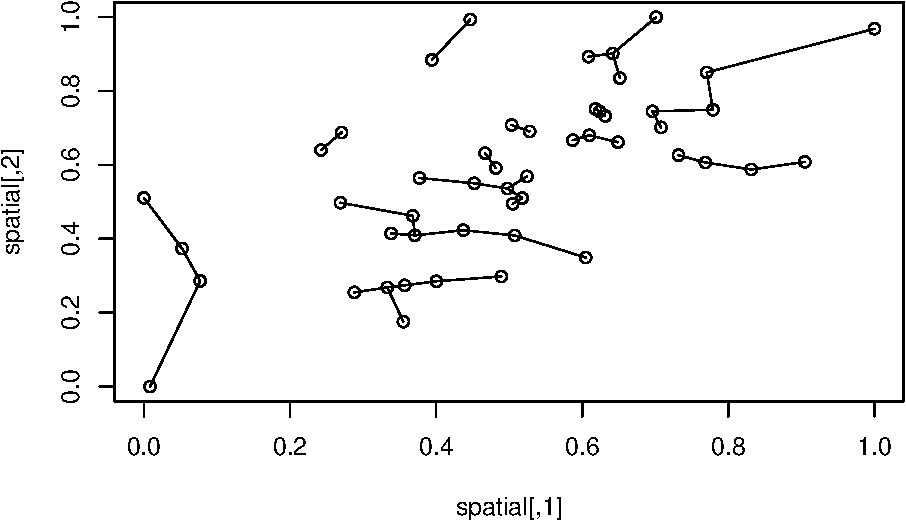
\includegraphics{05-cca-ex_files/figure-latex/unnamed-chunk-9-1.pdf}

The following gives the correlation between the original variables and the transformed variables

\begin{Shaded}
\begin{Highlighting}[]
\FunctionTok{print}\NormalTok{(cc.out}\SpecialCharTok{$}\NormalTok{scores}\SpecialCharTok{$}\NormalTok{corr.X.xscores)}
\end{Highlighting}
\end{Shaded}

\begin{verbatim}
##              [,1]          [,2]         [,3]
## growth -0.9798776  0.0006477883  0.199598477
## profit -0.9464085  0.3228847489 -0.007504408
## new    -0.9518620 -0.1863009724 -0.243414776
\end{verbatim}

\begin{Shaded}
\begin{Highlighting}[]
\FunctionTok{print}\NormalTok{(cc.out}\SpecialCharTok{$}\NormalTok{scores}\SpecialCharTok{$}\NormalTok{corr.Y.yscores)}
\end{Highlighting}
\end{Shaded}

\begin{verbatim}
##              [,1]       [,2]        [,3]
## create -0.6383313 -0.2156981 -0.65140953
## mech   -0.7211626  0.2375644  0.06773775
## abs    -0.6472493 -0.5013329  0.57422365
## math   -0.9440859  0.1975329  0.09422619
\end{verbatim}

\begin{Shaded}
\begin{Highlighting}[]
\FunctionTok{print}\NormalTok{(cc.out}\SpecialCharTok{$}\NormalTok{scores}\SpecialCharTok{$}\NormalTok{corr.X.yscores)}
\end{Highlighting}
\end{Shaded}

\begin{verbatim}
##              [,1]          [,2]         [,3]
## growth -0.9744713  0.0005688272  0.076567107
## profit -0.9411869  0.2835272081 -0.002878734
## new    -0.9466102 -0.1635921013 -0.093375287
\end{verbatim}

\begin{Shaded}
\begin{Highlighting}[]
\FunctionTok{print}\NormalTok{(cc.out}\SpecialCharTok{$}\NormalTok{scores}\SpecialCharTok{$}\NormalTok{corr.Y.xscores)}
\end{Highlighting}
\end{Shaded}

\begin{verbatim}
##              [,1]       [,2]        [,3]
## create -0.6348095 -0.1894059 -0.24988439
## mech   -0.7171837  0.2086069  0.02598458
## abs    -0.6436782 -0.4402237  0.22027544
## math   -0.9388771  0.1734549  0.03614570
\end{verbatim}

\begin{itemize}
\item
  Describe the first pair of canonical variables, give their correlation, and provide an interpretation.
\item
  Describe the second pair of canonical variables, and provide an interpretation.
\end{itemize}

\begin{enumerate}
\def\labelenumi{\arabic{enumi}.}
\setcounter{enumi}{1}
\tightlist
\item
  Attempt exam question 1 part (b) from the 2017-18 exam paper.
\end{enumerate}

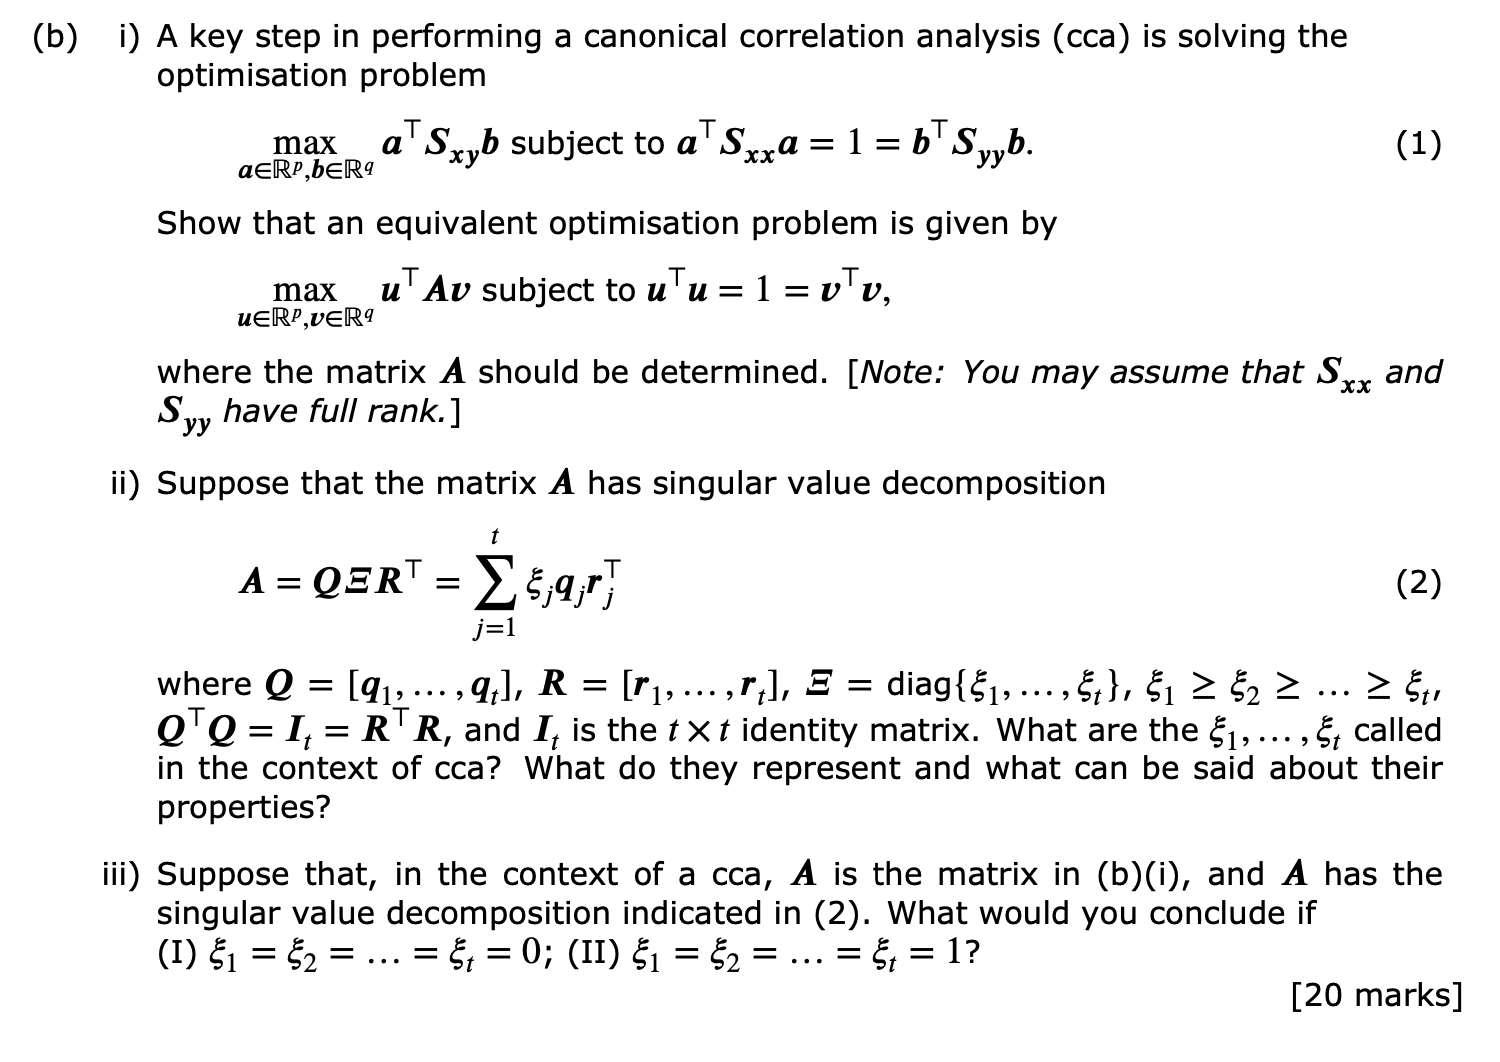
\includegraphics{figs/CCA_2017_18_Q1.png}

\begin{enumerate}
\def\labelenumi{\arabic{enumi}.}
\setcounter{enumi}{2}
\tightlist
\item
  Suppose that \(\mathbf z= (\mathbf x^\top \mathbf y^\top)^\top\) is a random vector, where both \(\mathbf x\) and \(\mathbf y\) are sub-vectors of dimension \(p\), so that \(\mathbf z\) is \((2p)\times 1\). Define
  \[{\mathbb{V}\operatorname{ar}}(\mathbf z)=\boldsymbol{\Sigma}_{\mathbf z\mathbf z}=\begin{pmatrix} \boldsymbol{\Sigma}_{\mathbf x\mathbf x} & \boldsymbol{\Sigma}_{\mathbf x\mathbf y}\\\boldsymbol{\Sigma}_{\mathbf y\mathbf x} & \boldsymbol{\Sigma}_{\mathbf y\mathbf y}  \end{pmatrix}.\]

  \begin{enumerate}
  \def\labelenumii{\roman{enumii}.}
  \tightlist
  \item
    Suppose that \(\mathbf y= \mathbf T\mathbf x\) where \(\mathbf T\) is a fixed matrix. Find \(\boldsymbol{\Sigma}_{\mathbf x\mathbf y}\) and \(\boldsymbol{\Sigma}_{\mathbf y\mathbf y}\) in terms of \(\boldsymbol{\Sigma}_{\mathbf x\mathbf x}\) and \(\mathbf T\).
  \item
    Assuming now that \(\mathbf T\) is an orthogonal matrix and \(\boldsymbol{\Sigma}_{\mathbf x\mathbf x}\) is of full rank, determine the singular values of the matrix \(\mathbf Q=\boldsymbol{\Sigma}_{\mathbf x\mathbf x}^{-1/2}\boldsymbol{\Sigma}_ {\mathbf x\mathbf y}\boldsymbol{\Sigma}_{\mathbf y\mathbf y}^{-1/2}\), and hence write down the canonical correlation coefficients.
  \item
    Suppose now that \(\mathbf T\) is non-singular but not orthogonal. Comment on whether the answer to part (b) changes.
  \end{enumerate}
\item
  We will now prove Proposition \ref{prp:svdopt3} by induction.
  The case for \(k=1\) was proved in Section \ref{cca1} in Proposition \ref{prp:svdmax2}. Assume the result is true for \(k\). Consider the objective
  \[\mathcal{L} = \mathbf a^\top \mathbf Q\mathbf b+ \sum_{i=1}^k \gamma_i\mathbf a^\top \mathbf a_i + \sum_{i=1}^k \mu_i\mathbf b^\top \mathbf b_i + \frac{\lambda_1}{2}(1-\mathbf a^\top\mathbf a)+ \frac{\lambda_2}{2}(1-\mathbf b^\top\mathbf b)\]
  where \(\lambda_i, \mu_i, \gamma_i\) are Lagrangian multipliers.

  \begin{enumerate}
  \def\labelenumii{\roman{enumii}.}
  \item
    By differentiating with respect to \(\mathbf a\) and \(\mathbf b\) and setting the derivative to zero show that
    \begin{align}
     \mathbf Q\mathbf b+ \sum\gamma_i \mathbf a_i - \lambda_1 \mathbf a&= 0 \label{eq:ex3a}\\
     \mathbf Q^\top\mathbf a+ \sum\mu_i \mathbf b_i - \lambda_2 \mathbf b&= 0. \label{eq:ex3b} 
     \end{align}
  \item
    By left multiplying the equations above by \(\mathbf a^\top\) and \(\mathbf b^\top\) respectively show that
    \[\lambda_1=\lambda_2 = \mathbf a^\top \mathbf Q\mathbf b.\]
  \item
    By left multiplying \eqref{eq:ex3a} by \(\mathbf a_i^\top\) show that \(\gamma_i=0\) for \(i=1, \ldots, k\). Show similarly that \(\mu_i =0\) for \(i=1, \ldots, k\).
  \item
    Finally, by copying the proof of Proposition \ref{prp:svdmax2}, prove Proposition \ref{prp:svdopt3}.
  \end{enumerate}
\item
  Show the mean of the cc variables \(\eta_k\) and \(\psi_k\) is zero. Prove Proposition \ref{prp:ccavar} giving the variance of covariance the cc variables.
\end{enumerate}

\chapter{Multidimensional Scaling (MDS)}\label{mds}

The videos for this chapter are available at:

\begin{itemize}
\tightlist
\item
  \href{https://mediaspace.nottingham.ac.uk/media/MDSA+Introduction/1_k5ofxt3k}{6.0 Introduction to MDS}
\item
  \href{https://mediaspace.nottingham.ac.uk/media/MDSA+Classical+MDS/1_0lz9sce2}{6.1 Classical MDS}
\item
  \href{https://mediaspace.nottingham.ac.uk/media/MDSA+Example+1/1_y5cp5ea6}{6.1 Example 1}
\item
  \href{https://mediaspace.nottingham.ac.uk/media/MDSA+Non-Euclidean+distance+matrices/1_nsh2vdgr}{6.1.1 Non-Euclidean distance matrices}
\item
  \href{https://mediaspace.nottingham.ac.uk/media/MDSA+Principal+Coordinate+Analysis/1_r07on81w}{6.1.2 Principal Coordinate Analysis}
\item
  \href{https://mediaspace.nottingham.ac.uk/media/MDSA+Similarity+matrices/1_wwuwwxk4}{6.2 Similarity measures}
\item
  \href{https://mediaspace.nottingham.ac.uk/media/MDSA+Binary+Attributes/1_jfx45kk0}{6.2.1 Binary attributes}
\item
  \href{https://mediaspace.nottingham.ac.uk/media/MDSA+Non+metric+MDS/1_jqzo1xi4}{6.3 Non-metric MDS}
\end{itemize}

In PCA, we start with \(n\) data points \(\mathbf x_i \in \mathbb{R}^p\), and then try to find a low dimensional projection of these points, e.g., \(\mathbf y_1, \ldots, \mathbf y_n \in \mathbb{R}^r\) with \(r<p\), in such a way that they minimize the reconstruction error (or maximize the variance).

The focus in \textbf{Multidimensional Scaling (MDS)} is somewhat different. Instead of being given the data \(\mathbf X\), our starting point is often a matrix of \textbf{distances} or \textbf{dissimilarities} between the data points, \(\mathbf D\). For example, if we have data on \(n\) different experimental units, then we would be given the distances \(d_{ij}\) between any pair of experimental units \(i\) and \(j\). We compile these into a \(n\times n\) \textbf{distance matrix} \(\mathbf D=(d_{ij}: \, i,j=1, \ldots , n)\).

The goal of MDS is to find a set of points in a low-dimensional Euclidean space \(\mathbb{R}^r\), usually \(\mathbb{R}\) or \(\mathbb{R}^2\), whose inter-point distances (or dissimilarities) are as close as possible to the \(d_{ij}\). That is, we want to find \(\mathbf y_1, \ldots, \mathbf y_n \in \mathbb{R}^r\) whose distance matrix is approximately \(\mathbf D\), i.e., for which
\[\operatorname{distance}(\mathbf y_i, \mathbf y_j) \approx d_{ij}.\]
In other words, we are trying to create a spatial representation of the data, \(\mathbf y_1, \ldots, \mathbf y_n\), from a distance matrix \(\mathbf D\). The vectors \(\mathbf y_i\) have no meaning by themselves, but by visualising their spatial pattern we can hope to learn something about the dataset represented by \(\mathbf D\).

If we define the errors in terms of a square distance, then we can write the goal of MDS as the following optimization problem:
\begin{align}
\mbox{Find} \quad& \mathbf y_1, \ldots, \mathbf y_n \in \mathbb{R}^r\\
\mbox{to minimize} \quad &\sum_{i=1}^n \sum_{j=1}^n (d_{ij} - d(\mathbf y_i, \mathbf y_j))^2.\label{eq:mdsopt}
\end{align}

As an illustrative example, consider the location of some of England's cities.

\includegraphics{06-mds_files/figure-latex/unnamed-chunk-1-1.pdf}

If we are told their latitude and longitude, it is easy to calculate the distances between the cities. I.e., given the latitude and longitude of each city, \(\mathbf x_i\), we can compute the distance matrix between pairs of cities \(\mathbf D\):

\begin{table}
\centering\begingroup\fontsize{7}{9}\selectfont

\begin{tabular}{lrrrrrrrrrrrrr}
\toprule
  & London & Birmingham & Manchester & Leeds & Newcastle & Liverpool & Portsmouth & Southampton & Nottingham & Bristol & Sheffield & Norwich & Plymouth\\
\midrule
London & 0 & 163 & 262 & 273 & 403 & 286 & 103 & 112 & 175 & 170 & 228 & 159 & 308\\
Birmingham & 163 & 0 & 114 & 149 & 282 & 125 & 195 & 179 & 73 & 124 & 105 & 217 & 281\\
Manchester & 262 & 114 & 0 & 58 & 174 & 50 & 308 & 293 & 94 & 227 & 53 & 255 & 369\\
Leeds & 273 & 149 & 58 & 0 & 135 & 105 & 335 & 323 & 98 & 271 & 47 & 230 & 420\\
Newcastle & 403 & 282 & 174 & 135 & 0 & 199 & 469 & 458 & 231 & 401 & 181 & 328 & 542\\
\addlinespace
Liverpool & 286 & 125 & 50 & 105 & 199 & 0 & 317 & 299 & 132 & 219 & 101 & 299 & 346\\
Portsmouth & 103 & 195 & 308 & 335 & 469 & 317 & 0 & 24 & 239 & 127 & 288 & 261 & 221\\
Southampton & 112 & 179 & 293 & 323 & 458 & 299 & 24 & 0 & 229 & 103 & 276 & 268 & 202\\
Nottingham & 175 & 73 & 94 & 98 & 231 & 132 & 239 & 229 & 0 & 193 & 53 & 169 & 353\\
Bristol & 170 & 124 & 227 & 271 & 401 & 219 & 127 & 103 & 193 & 0 & 228 & 296 & 162\\
\addlinespace
Sheffield & 228 & 105 & 53 & 47 & 181 & 101 & 288 & 276 & 53 & 228 & 0 & 203 & 382\\
Norwich & 159 & 217 & 255 & 230 & 328 & 299 & 261 & 268 & 169 & 296 & 203 & 0 & 453\\
Plymouth & 308 & 281 & 369 & 420 & 542 & 346 & 221 & 202 & 353 & 162 & 382 & 453 & 0\\
\bottomrule
\end{tabular}
\endgroup{}
\end{table}

But can we do the reverse and construct a map from the distance matrix? This is the aim of multidimensional scaling:
MDS constructs a set of points, \(\mathbf y_1, \ldots, \mathbf y_n\), that have distances between them given by the distance matrix \(\mathbf D\). In other words, it creates a map with a set of coordinates for which the distances between points are approximately the same as in the real data.

Of course, this illustrative example is not very interesting, as the original data (the city locations) are only two-dimensional, but in problems with high dimensional data, finding a way to
represent the points in a low-dimensional space will make visualization and statistical analysis easier. We shall see, perhaps unsurprisingly, that there is a close connection between MDS and PCA.

\subsubsection*{Notation}\label{notation-2}
\addcontentsline{toc}{subsubsection}{Notation}

There are many ways to compute distances between points. For example, you may have studied metrics previously, which are distance functions that satisfy certain axioms. In MDS, we do not need to work with distances that are metrics (although sometimes we do), and instead we only require that distances satisfy a weaker set of conditions:

\begin{definition}
\protect\hypertarget{def:distanceD}{}\label{def:distanceD}

The \(n \times n\) matrix \(\mathbf D=(d_{ij})_{i,j=1}^n\) is a \textbf{distance matrix} (sometimes called a \textbf{dissimilarity matrix}) if

\begin{enumerate}
\def\labelenumi{\arabic{enumi}.}
\tightlist
\item
  \(d_{ij}\geq 0\) for all \(i, j=1,\ldots,n\).
\item
  \(d_{ii}=0\) for \(i=1,\ldots, n\) and
\item
  \(\mathbf D=\mathbf D^\top\), i.e., \(\mathbf D\) is symmetric (\(d_{ij}=d_{ji}\)).
\end{enumerate}

\end{definition}

Note that we do not require distances to necessarily satisfy the triangle inequality
\begin{equation}
d_{ik} \leq d_{ij}+d_{jk}.
\label{eq:triangle}
\end{equation}
A distance function which always satisfies the triangle inequality is called a \textbf{metric distance}
or just a \textbf{metric}. A distance function which does not always satisfy the triangle inequality is called a
\textbf{non-metric} distance.

There are many ways to measure distance. Two common choices of metric distances are

\begin{itemize}
\tightlist
\item
  Euclidean distance \(||\mathbf x-\mathbf x'||_2\), also know as the `crow flies' distance.
\item
  \(L_1\) distance \(||\mathbf x-\mathbf x'||_1\), sometimes called the Manhattan or taxicab metric.
\end{itemize}

But for the city data, we could also consider distance by road, i.e., we could measure the minimum distance by road between each pair of cities. This would satisfy the axioms for being a distance, but is not a metric distance

The choice of which distance is appropriate is problem specific (see section \ref{similarity} for an example). The focus in this chapter is on Euclidean distance, as this leads to an explicit mathematical solution to the optimization problem \eqref{eq:mdsopt}. However, note that MDS techniques have also been developed for non-Euclidean distances.

\section{Classical MDS}\label{classical-mds}

Classical MDS is based upon \textbf{Euclidean distances}:
\[d(\mathbf x, \mathbf x') = ||\mathbf x-\mathbf x'||_2 = \sqrt{(\mathbf x-\mathbf x')^\top (\mathbf x-\mathbf x')}.\]

Since Euclidean distances satisfy the triangle
inequality \eqref{eq:triangle}, it follows that Euclidean distance is a metric distance. In general, any distance derived from a norm is a metric distance.

\begin{definition}
\protect\hypertarget{def:euclideanD}{}\label{def:euclideanD}Suppose \(\mathbf D\) is an \(n\times n\) distance matrix. We say \(\mathbf D\) is a \textbf{Euclidean distance matrix}
if there is a set of points \(\mathbf x_1,\ldots , \mathbf x_n \in \mathbb{R}^p\) for some \(p\), such that
\[
d_{ij}=\vert \vert \mathbf x_i -\mathbf x_j \vert \vert_2 =\sqrt{(\mathbf x_i-\mathbf x_j)^\top (\mathbf x_i-\mathbf x_j)}.
\]
\end{definition}

In classical MDS, we don't work directly with the distance matrix, but with the centred inner product matrix.

\begin{definition}
\protect\hypertarget{def:unnamed-chunk-3}{}\label{def:unnamed-chunk-3}Given a distance matrix \({\mathbf D}=\{d_{ij}\}_{i,j=1}^n\),
the \textbf{centred inner-product matrix} (also called the \textbf{centred-Gram matrix}) is
\begin{equation}
{\mathbf B}={\mathbf H} \mathbf A{\mathbf H},
\label{eq:defB}
\end{equation}
where
\(\mathbf A\) is the matrix of negative square distances divided by two:
\begin{equation}
\mathbf A=\{a_{ij}\}_{i,j=1}^n,  \quad \text{where} \qquad a_{ij}=-\frac{1}{2}d_{ij}^2
\label{eq:defA}
\end{equation}
and \(\mathbf H\) is the \(n \times n\) \textbf{centering matrix} (see Section \ref{centering-matrix}).

Another way of writing \(\mathbf A\) is as
\[\mathbf A= -\frac{1}{2}\mathbf D\odot \mathbf D\]
where \(\odot\) denotes the \href{https://en.wikipedia.org/wiki/Hadamard_product_(matrices)}{Hadamard (or element-wise) product} of two matrices.
\end{definition}

We can think of \(\mathbf B\) as a matrix of similarities for the data.
The reason for this, and for why we call \(\mathbf B\) the centred inner product matrix will become clear after we state the main result of this chapter.

\subsubsection*{Main result}\label{main-result-1}
\addcontentsline{toc}{subsubsection}{Main result}

We now present the key result for classical MDS. It says that a distance matrix \(\mathbf D\) is a \emph{Euclidean} distance matrix if and only if the corresponding centred inner product matrix \(\mathbf B\) is positive semi-definite. It also tells us how given data \(\mathbf X\) we can compute \(\mathbf B\) directly from \(\mathbf X\). Conversely, and more importantly, it tells us how given \(\mathbf B\) we can compute some data points \(\mathbf X\) that have corresponding Euclidean distance matrix \(\mathbf D\).

\begin{theorem}
\protect\hypertarget{thm:five1}{}\label{thm:five1}

Let \(\mathbf D\) denote an \(n \times n\) distance matrix with corresponding centred inner-product matrix \(\mathbf B=-\frac{1}{2}\mathbf H(\mathbf D\odot\mathbf D)\mathbf H.\)

\begin{enumerate}
\def\labelenumi{\arabic{enumi}.}
\item
  If \(\mathbf D\) is a \textbf{Euclidean} distance matrix for the sample of \(n\) vectors \(\mathbf x_1,\ldots , \mathbf x_n\), then
  \begin{equation}
  \mathbf B= ({\mathbf H} {\mathbf X})({\mathbf H} {\mathbf X})^\top.
  \label{eq:bijB}
  \end{equation}
  Thus \(\mathbf B\) is positive semi-definite.
\item
  Suppose \(\mathbf B\) is positive semi-definite with eigenvalues \(\lambda_1 \geq \lambda_2 \cdots \geq \lambda_k > 0\) and that it has spectral decomposition \(\mathbf B={\mathbf U} {\pmb \Lambda}{\mathbf U}^\top\), where \({\pmb \Lambda}=\text{diag}\{\lambda_1 \ldots \lambda_k\}\) and \(\mathbf U\) is \(n \times k\) and satisfies \({\mathbf U}^\top {\mathbf U}={\mathbf I}_k\). Then
  \[{\mathbf X}=[\mathbf x_1, \ldots , \mathbf x_n]^\top={\mathbf U}{\pmb \Lambda}^{1/2}\]
  is an \(n \times k\) data matrix which has \textbf{Euclidean} distance matrix \(\mathbf D\).

  Moreover, for this data matrix \(\bar{\mathbf x}={\mathbf 0}_k\) and \(\mathbf B\) represents the inner product matrix with elements given by \eqref{eq:bijB}.
\end{enumerate}

\end{theorem}

For part 1. we may equivalently write
\begin{equation}
b_{ij}=(\mathbf x_i-\bar{\mathbf x})^\top (\mathbf x_j - \bar{\mathbf x}), \qquad i,j=1,\ldots , n,
\end{equation}
where \(\bar{\mathbf x}=n^{-1}\sum_{i=1}^n \mathbf x_i\) is the sample mean vector.
This illustrates why we call \(\mathbf B\) the \emph{centred inner-product} matrix: \(\mathbf H\mathbf X\) is the centred data matrix, and \((\mathbf H\mathbf X)(\mathbf H\mathbf X)^\top\) thus contains the inner product of each pair of centred vectors.

We think of \(\mathbf B\) as a matrix of pair-wise \textbf{similarities} between the data points. The inner product \[\langle \mathbf x_i-\bar{\mathbf x}, \;\mathbf x_j - \bar{\mathbf x} \rangle=(\mathbf x_i-\bar{\mathbf x})^\top (\mathbf x_j - \bar{\mathbf x})\] is large if \(\mathbf x_i\) is similar to \(\mathbf x_j\), and small if they are very different. It may help to think back to the geometric interpretation of inner products from Section \ref{normed}.

\begin{proof}
You will prove this result in the example sheets.
\end{proof}

\begin{corollary}
\protect\hypertarget{cor:unnamed-chunk-4}{}\label{cor:unnamed-chunk-4}The distance matrix \(\mathbf D\) is a Euclidean distance matrix if and only if the corresponding centred inner-product matrix \(\mathbf B\) is a positive semi-definite matrix.
\end{corollary}

These results say that if \(\mathbf D\) is a Euclidean distance matrix (which we can check by testing whether \(\mathbf B\) is positive semi-definite), then we can find a set of \(n\) points \(\mathbf x_1, \ldots, \mathbf x_n\in \mathbb{R}^k\) which have interpoint distances \(\mathbf D\). The dimension of the points is given by the rank of \(\mathbf B\).

\subsubsection*{Example 1}\label{example-1}
\addcontentsline{toc}{subsubsection}{Example 1}

Consider the five points in \(\mathbb{R}^2\):
\[
\mathbf x_1=(0,0)^\top,  \mathbf x_2 =(1,0)^\top, \quad \mathbf x_3 =(0,1)^\top
\]
\[
\mathbf x_4 =(-1,0)^\top \quad \text{and} \quad \mathbf x_5=(0,-1)^\top.
\]

The resulting distance matrix is
\[
\mathbf D=\left [ \begin{array}{ccccc}
0&1&1&1&1\\
1&0&\sqrt{2}&2&\sqrt{2}\\
1&\sqrt{2}&0&\sqrt{2}&2\\
1&2&\sqrt{2}&0&\sqrt{2}\\
1&\sqrt{2}&2&\sqrt{2}&0
\end{array} \right ].
\]

The aim of MDS is to construct a set of \(5\) points in \(\mathbb{R}^k\) for some choice of \(k\), that have interpoint distances given by \(\mathbf D\).

Using \eqref{eq:defA} first to calculate \(\mathbf A\), and then using \eqref{eq:defB} to calculate \(\mathbf B\), we find that
\[
\mathbf A=-\left [ \begin{array}{ccccc}
0&0.5&0.5&0.5&0.5\\
0.5&0&1&2&1\\
0.5&1&0&1&2\\
0.5&2&1&0&1\\
0.5&1&2&1&0
\end{array} \right ]
\]
and
\[
\mathbf B=\left [ \begin{array}{ccccc}
 0& 0&0&0&0\\
0&1&0&-1&0\\
0&0&1&0&-1\\
0&-1&0&1&0\\
0&0&-1&0&1
\end{array} \right ].
\]

In R we can compute these as follows:

\begin{Shaded}
\begin{Highlighting}[]
\NormalTok{X }\OtherTok{\textless{}{-}} \FunctionTok{matrix}\NormalTok{(}\FunctionTok{c}\NormalTok{(}\DecValTok{0}\NormalTok{,}\DecValTok{0}\NormalTok{,}
              \DecValTok{1}\NormalTok{,}\DecValTok{0}\NormalTok{,}
              \DecValTok{0}\NormalTok{,}\DecValTok{1}\NormalTok{,}
              \SpecialCharTok{{-}}\DecValTok{1}\NormalTok{,}\DecValTok{0}\NormalTok{,}
              \DecValTok{0}\NormalTok{,}\SpecialCharTok{{-}}\DecValTok{1}\NormalTok{), }\AttributeTok{nc=}\DecValTok{2}\NormalTok{, }\AttributeTok{byrow=}\ConstantTok{TRUE}\NormalTok{)}
\NormalTok{D }\OtherTok{\textless{}{-}} \FunctionTok{as.matrix}\NormalTok{(}\FunctionTok{dist}\NormalTok{(X, }\AttributeTok{upper=}\NormalTok{T, }\AttributeTok{diag=}\NormalTok{T))}
\NormalTok{A }\OtherTok{\textless{}{-}} \SpecialCharTok{{-}}\NormalTok{D}\SpecialCharTok{\^{}}\DecValTok{2}\SpecialCharTok{/}\DecValTok{2} 
\CommentTok{\# note D\^{}2 does element wise operations, different to D\%*\%D}
\NormalTok{H }\OtherTok{\textless{}{-}} \FunctionTok{diag}\NormalTok{(}\DecValTok{5}\NormalTok{) }\SpecialCharTok{{-}} \DecValTok{1}\SpecialCharTok{/}\DecValTok{5} \SpecialCharTok{*} \FunctionTok{matrix}\NormalTok{(}\FunctionTok{rep}\NormalTok{(}\DecValTok{1}\NormalTok{,}\DecValTok{5}\NormalTok{), }\AttributeTok{nc=}\DecValTok{1}\NormalTok{)}\SpecialCharTok{\%*\%}\FunctionTok{matrix}\NormalTok{(}\FunctionTok{rep}\NormalTok{(}\DecValTok{1}\NormalTok{,}\DecValTok{5}\NormalTok{), }\AttributeTok{nr=}\DecValTok{1}\NormalTok{)}
\NormalTok{B }\OtherTok{\textless{}{-}}\NormalTok{ H}\SpecialCharTok{\%*\%}\NormalTok{ A}\SpecialCharTok{\%*\%}\NormalTok{H }\CommentTok{\#check this matches  (H \%*\% X) \%*\% t(H \%*\% X)}
\end{Highlighting}
\end{Shaded}

You should check that \(\mathbf H\mathbf A\mathbf H\) is the same as \((\mathbf H\mathbf X)(\mathbf H\mathbf X)^\top\), thus verifying part 1. of Theorem \ref{thm:five1}. Note that there will be very small differences (\(\sim 10^{-16}\)) due to numerical errors.

How do we construct, using only the information in \(\mathbf B\), a set of \(5\) points that have Euclidean interpoint distances given by \(\mathbf D\)?
Firstly, we need to compute the spectral decomposition of \(\mathbf B\). The eigenvalues of \(\mathbf B\) are
\[
\lambda_1=\lambda_2=2 \qquad \text{and} \qquad \lambda_3=\lambda_4=\lambda_5=0.
\]

Thus \(\mathbf B\) is positive semi-definite, and so
by Theorem \ref{thm:five1}, \(\mathbf D\) must be a Euclidean distance matrix. This isn't a surprise to us because we created \(\mathbf D\) ourselves in this case.

There are two positive eigenvalues, and so \(\mathbf B\) has rank 2, and the theorem tells us we can construct points \(\mathbf x_i \in \mathbb{R}^2\), i.e., points in 2-dimensional space.

To find the points we need to find the matrix of orthogonal unit eigenvectors of \(\mathbf B\), which we denoted as \(\mathbf U\) in the theorem.
Because we have a repeated eigenvalue (\(\lambda=2\) has \emph{multiplicity} 2), the eigenspace associated with \(\lambda=2\) is a two dimensional space.
There is not a unique pair of orthogonal unit eigenvectors spanning this space (there are an infinite number of possible pairs).
The sparsest choice (i.e.~the one with most zero elements) is
\[
\mathbf u_1= \begin{pmatrix}0 \\ 0 \\ -\frac{1}{\sqrt{2}} \\ 0 \\ -\frac{1}{\sqrt{2}} \end{pmatrix} \qquad
\text{and} \qquad \mathbf u_2 =\begin{pmatrix}0 \\ -\frac{1}{\sqrt{2}} \\ 0 \\ \frac{1}{\sqrt{2}}\\ 0 \end{pmatrix}.
\]

Note that if we compute these in R, you may well get different eigenvectors, but the subspace described by the pair of vectors will be the same.

\begin{Shaded}
\begin{Highlighting}[]
\FunctionTok{eigen}\NormalTok{(B)}\SpecialCharTok{$}\NormalTok{values }\CommentTok{\#using B = H\%*\% A\%*\%H }
\end{Highlighting}
\end{Shaded}

\begin{verbatim}
## [1]  2.000000e+00  2.000000e+00  1.207037e-15  3.331224e-16 -2.775558e-17
\end{verbatim}

\begin{Shaded}
\begin{Highlighting}[]
\FunctionTok{eigen}\NormalTok{(B)}\SpecialCharTok{$}\NormalTok{vectors[,}\DecValTok{1}\SpecialCharTok{:}\DecValTok{2}\NormalTok{]}
\end{Highlighting}
\end{Shaded}

\begin{verbatim}
##            [,1]       [,2]
## [1,]  0.0000000  0.0000000
## [2,] -0.6916609  0.1469869
## [3,] -0.1469869 -0.6916609
## [4,]  0.6916609 -0.1469869
## [5,]  0.1469869  0.6916609
\end{verbatim}

\begin{Shaded}
\begin{Highlighting}[]
\NormalTok{B2 }\OtherTok{\textless{}{-}}\NormalTok{ (H }\SpecialCharTok{\%*\%}\NormalTok{ X) }\SpecialCharTok{\%*\%} \FunctionTok{t}\NormalTok{(H }\SpecialCharTok{\%*\%}\NormalTok{ X) }\CommentTok{\# alternative way of computing B}
\FunctionTok{eigen}\NormalTok{(B2)}\SpecialCharTok{$}\NormalTok{values}
\end{Highlighting}
\end{Shaded}

\begin{verbatim}
## [1] 2.000000e+00 2.000000e+00 1.110223e-15 1.110223e-15 0.000000e+00
\end{verbatim}

\begin{Shaded}
\begin{Highlighting}[]
\FunctionTok{eigen}\NormalTok{(B2)}\SpecialCharTok{$}\NormalTok{vectors[,}\DecValTok{1}\SpecialCharTok{:}\DecValTok{2}\NormalTok{]}
\end{Highlighting}
\end{Shaded}

\begin{verbatim}
##            [,1]       [,2]
## [1,]  0.0000000  0.0000000
## [2,]  0.0000000 -0.7071068
## [3,] -0.7071068  0.0000000
## [4,]  0.0000000  0.7071068
## [5,]  0.7071068  0.0000000
\end{verbatim}

We can now compute the coordinates of five points in \(\mathbb{R}^2\) which have Euclidean distance matrix, \(\mathbf D,\) by
\[
\mathbf U\boldsymbol \Lambda^{1/2}=\sqrt{2}[\mathbf u_1 , \mathbf u_2].\]

Note again that these coordinates are not unique as any rotation or translation of them will have the same distance matrix. In particular, when doing computations in R we may find different answers depending upon how we do the computation. So for example, if we use the eigendecompostion of \(\mathbf B= \mathbf H\mathbf A\mathbf H\)

\begin{Shaded}
\begin{Highlighting}[]
\NormalTok{B.eig }\OtherTok{\textless{}{-}} \FunctionTok{eigen}\NormalTok{(B)}
\NormalTok{Y }\OtherTok{\textless{}{-}}\FunctionTok{sqrt}\NormalTok{(B.eig}\SpecialCharTok{$}\NormalTok{values[}\DecValTok{1}\SpecialCharTok{:}\DecValTok{2}\NormalTok{])}\SpecialCharTok{*}\NormalTok{B.eig}\SpecialCharTok{$}\NormalTok{vectors[,}\DecValTok{1}\SpecialCharTok{:}\DecValTok{2}\NormalTok{]}
\end{Highlighting}
\end{Shaded}

we find
\[\begin{pmatrix}0&0 \\-0.978&0.208 \\-0.208&-0.978 \\0.978&-0.208 \\0.208&0.978 \\\end{pmatrix}.\]
Whereas if we use the eigen decomposition of \((\mathbf H\mathbf X)(\mathbf H\mathbf X)^\top\) we find a different set of points:

\begin{Shaded}
\begin{Highlighting}[]
\NormalTok{B2.eig }\OtherTok{\textless{}{-}} \FunctionTok{eigen}\NormalTok{(B2)}
\NormalTok{Y2 }\OtherTok{\textless{}{-}}\FunctionTok{sqrt}\NormalTok{(B2.eig}\SpecialCharTok{$}\NormalTok{values[}\DecValTok{1}\SpecialCharTok{:}\DecValTok{2}\NormalTok{])}\SpecialCharTok{*}\NormalTok{B2.eig}\SpecialCharTok{$}\NormalTok{vectors[,}\DecValTok{1}\SpecialCharTok{:}\DecValTok{2}\NormalTok{]}
\end{Highlighting}
\end{Shaded}

\[\begin{pmatrix}0&0 \\0&-1 \\-1&0 \\0&1 \\1&0 \\\end{pmatrix}.\]

The distance matrices for both sets of points are equal to \(\mathbf D\)

\begin{Shaded}
\begin{Highlighting}[]
\FunctionTok{signif}\NormalTok{(}\FunctionTok{dist}\NormalTok{(Y, }\AttributeTok{upper=}\NormalTok{T, }\AttributeTok{diag=}\NormalTok{T),}\DecValTok{2}\NormalTok{) }\CommentTok{\# should agree with D.}
\end{Highlighting}
\end{Shaded}

\begin{verbatim}
##     1   2   3   4   5
## 1 0.0 1.0 1.0 1.0 1.0
## 2 1.0 0.0 1.4 2.0 1.4
## 3 1.0 1.4 0.0 1.4 2.0
## 4 1.0 2.0 1.4 0.0 1.4
## 5 1.0 1.4 2.0 1.4 0.0
\end{verbatim}

\begin{Shaded}
\begin{Highlighting}[]
\FunctionTok{signif}\NormalTok{(}\FunctionTok{dist}\NormalTok{(Y2, }\AttributeTok{upper=}\NormalTok{T, }\AttributeTok{diag=}\NormalTok{T),}\DecValTok{2}\NormalTok{) }\CommentTok{\# should agree with D.}
\end{Highlighting}
\end{Shaded}

\begin{verbatim}
##     1   2   3   4   5
## 1 0.0 1.0 1.0 1.0 1.0
## 2 1.0 0.0 1.4 2.0 1.4
## 3 1.0 1.4 0.0 1.4 2.0
## 4 1.0 2.0 1.4 0.0 1.4
## 5 1.0 1.4 2.0 1.4 0.0
\end{verbatim}

Finally, note that as always, there is an R command that will do all of this work for us

\begin{Shaded}
\begin{Highlighting}[]
\NormalTok{Y.mds }\OtherTok{\textless{}{-}} \FunctionTok{cmdscale}\NormalTok{(D, }\AttributeTok{eig=}\ConstantTok{TRUE}\NormalTok{) }\CommentTok{\#Classical MultiDimensional Scaling}
\end{Highlighting}
\end{Shaded}

giving the set of points
\[\begin{pmatrix}0&0 \\1&0 \\0&-1 \\-1&0 \\0&1 \\\end{pmatrix}.\]

If we plot the original data points \(\mathbf X\), along with the three sets of reconstructed data points \texttt{Y}, \texttt{Y2}, and \texttt{Y.mds} we can see that they are essentially the same, apart from being rotatated or reordered.

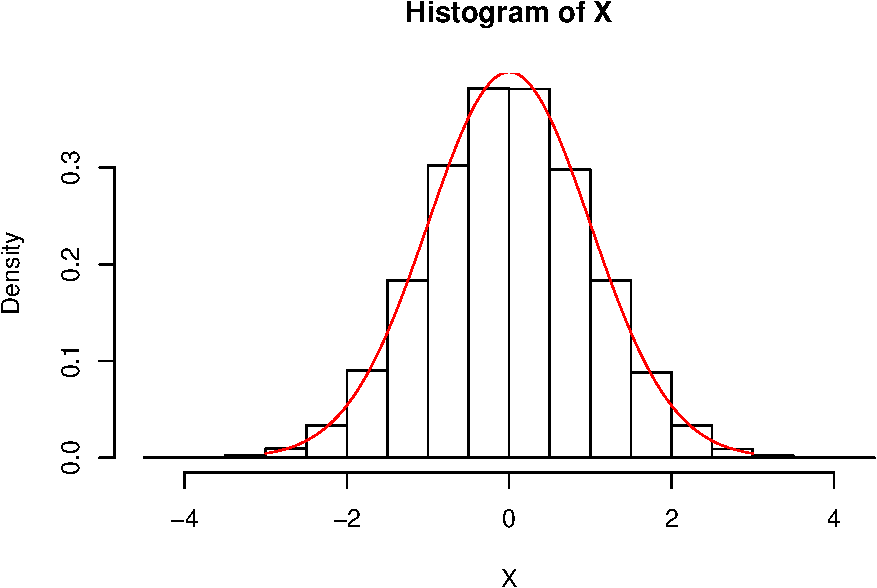
\includegraphics{06-mds_files/figure-latex/unnamed-chunk-13-1.pdf}

\subsubsection*{Example 2}\label{example-2}
\addcontentsline{toc}{subsubsection}{Example 2}

If we apply the \texttt{cmdscale} to the distances between UK cities from the introduction, we get the `coordinates' shown below.

\includegraphics{06-mds_files/figure-latex/unnamed-chunk-14-1.pdf}

This `map' is essentially correct, but it is rotated \(90^\circ\) and the `coordinates' have mean zero.

\subsection{Non-Euclidean distance matrices}\label{non-euclidean-distance-matrices}

Proposition \ref{thm:five1} may be useful even if \({\mathbf D}\) is not a \emph{Euclidean} distance matrix (in which case \(\mathbf B\) will have some negative eigenvalues). For example, this can occur if the distances between points is measured with errror.

In this case, instead of using \(\mathbf B\) in Proposition \ref{thm:five1} we can use its positive part. If \(\mathbf B\) has spectral decomposition \(\sum_{j=1}^p \lambda_j \mathbf u_j \mathbf u_j^\top\), then its positive definite part is defined by
\[
\mathbf B_{\text{pos}}=\sum_{j: \, \lambda_j>0} \lambda_j \mathbf u_j \mathbf u_j^\top.
\]
In other words, we sum over those \(j\) such that \(\lambda_j\) is positive.

Then \(\mathbf B_{\text{pos}}\) is positive semi-definite and so we can use part 2. of Theorem \ref{thm:five1} to determine a Euclidean configuration of points which has centred inner-product matrix \(\mathbf B_{\text{pos}}\). Then, provided the negative eigenvalues are small in absolute value relative to the positive eigenvalues, the inter-point distances of the new points in Euclidean space should provide a good approximation to the original inter-point distances \((d_{ij})\).

\subsubsection*{Example 3}\label{example-3}
\addcontentsline{toc}{subsubsection}{Example 3}

Let's now look at a case for which \(\mathbf B\) isn't positive definite. We'll create this by modifying the distance matrix we had before:

\[\mathbf D_2 = \begin{pmatrix}0&0.5&1&1&1 \\0.5&0&1.41&2&1.41 \\1&1.41&0&1.41&2 \\1&2&1.41&0&1.41 \\1&1.41&2&1.41&0 \\\end{pmatrix}.\]
This is a distance matrix, but is it a \emph{Euclidean} distance matrix? I.e., is there a set of vectors \(\mathbf x_1, \ldots, \mathbf x_5\) which have Euclidean distances between them given by \(\mathbf D_2\)?

If we look at the eigenvalues of the centred inner-product matrix \(\mathbf B\) associated with \(\mathbf D_2\), then we find that it has negative eigenvalues, and is thus not positive semi-definite. Thus by Theorem \ref{thm:five1} \(\mathbf D_2\) is not a \emph{Euclidean} distance matrix.

\begin{Shaded}
\begin{Highlighting}[]
\NormalTok{D2 }\OtherTok{\textless{}{-}}\NormalTok{ D}
\NormalTok{D2[}\DecValTok{2}\NormalTok{,}\DecValTok{1}\NormalTok{]}\OtherTok{\textless{}{-}}\FloatTok{0.5}
\NormalTok{D2[}\DecValTok{1}\NormalTok{,}\DecValTok{2}\NormalTok{]}\OtherTok{\textless{}{-}}\NormalTok{D2[}\DecValTok{2}\NormalTok{,}\DecValTok{1}\NormalTok{]}
\NormalTok{A2 }\OtherTok{\textless{}{-}} \SpecialCharTok{{-}}\NormalTok{D2}\SpecialCharTok{\^{}}\DecValTok{2}\SpecialCharTok{/}\DecValTok{2} 
\NormalTok{B2 }\OtherTok{\textless{}{-}}\NormalTok{ H}\SpecialCharTok{\%*\%}\NormalTok{ A2}\SpecialCharTok{\%*\%}\NormalTok{H }
\FunctionTok{eigen}\NormalTok{(B2)}\SpecialCharTok{$}\NormalTok{values}
\end{Highlighting}
\end{Shaded}

\begin{verbatim}
## [1]  2.026016e+00  2.000000e+00  1.004310e-01 -7.216450e-16 -2.764470e-01
\end{verbatim}

We can still use classical multidimensional scaling to find a set of points \(\mathbf x_1, \ldots, \mathbf x_5\) that have distances approximately given by \(\mathbf D_2\).
\texttt{cmdscale} allows us to specify the dimension of the points \(\mathbf x_i\). If we pick \(\dim(\mathbf x)=2\) then it gives us the set of points

\begin{Shaded}
\begin{Highlighting}[]
\FunctionTok{cmdscale}\NormalTok{(D2, }\AttributeTok{k=}\DecValTok{2}\NormalTok{)}
\end{Highlighting}
\end{Shaded}

\begin{verbatim}
##          [,1]          [,2]
## 1 -0.13881300  1.449541e-15
## 2 -0.97216111  1.011091e-14
## 3  0.04112656 -1.000000e+00
## 4  1.02872100 -1.018790e-14
## 5  0.04112656  1.000000e+00
\end{verbatim}

which have a distance matrix that approximates \(\mathbf D_2\), but does not equal it. By using a different number of dimensions, we may be able to get a set of points that have a distance matrix closer to \(\mathbf D_2\), but we will not be able to find a set of \(5\) points that have a distance matrix exactly equal to \(\mathbf D_2\).

To do this ourselves (i.e., not using \texttt{cmdscale}) we can use the commands

\begin{Shaded}
\begin{Highlighting}[]
\NormalTok{U }\OtherTok{\textless{}{-}} \FunctionTok{eigen}\NormalTok{(B2)}\SpecialCharTok{$}\NormalTok{vectors[,}\DecValTok{1}\SpecialCharTok{:}\DecValTok{2}\NormalTok{]}
\NormalTok{Lambda\_sqrt }\OtherTok{\textless{}{-}} \FunctionTok{diag}\NormalTok{(}\FunctionTok{sqrt}\NormalTok{(}\FunctionTok{eigen}\NormalTok{(B2)}\SpecialCharTok{$}\NormalTok{values[}\DecValTok{1}\SpecialCharTok{:}\DecValTok{2}\NormalTok{]))}
\NormalTok{Y }\OtherTok{\textless{}{-}}\NormalTok{ U }\SpecialCharTok{\%*\%}\NormalTok{ Lambda\_sqrt}
\FunctionTok{dist}\NormalTok{(Y)}
\end{Highlighting}
\end{Shaded}

\begin{verbatim}
##           1         2         3         4
## 2 0.8333481                              
## 3 1.0160602 1.4236404                    
## 4 1.1675340 2.0008821 1.4054689          
## 5 1.0160602 1.4236404 2.0000000 1.4054689
\end{verbatim}

\begin{Shaded}
\begin{Highlighting}[]
\FunctionTok{dist}\NormalTok{(}\FunctionTok{cmdscale}\NormalTok{(D2,}\AttributeTok{k=}\DecValTok{2}\NormalTok{))}
\end{Highlighting}
\end{Shaded}

\begin{verbatim}
##           1         2         3         4
## 2 0.8333481                              
## 3 1.0160602 1.4236404                    
## 4 1.1675340 2.0008821 1.4054689          
## 5 1.0160602 1.4236404 2.0000000 1.4054689
\end{verbatim}

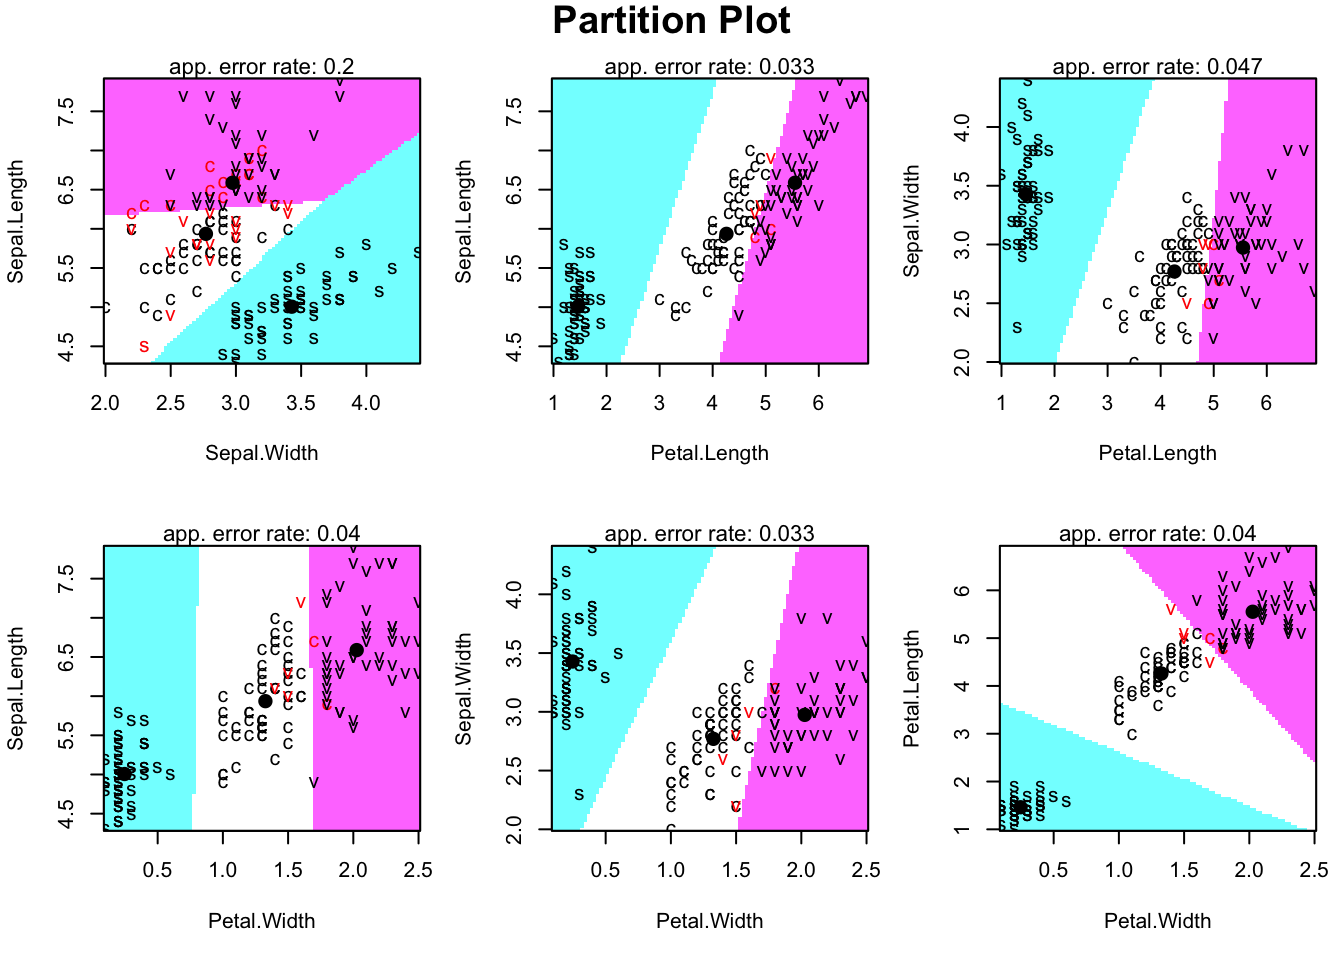
\includegraphics{06-mds_files/figure-latex/unnamed-chunk-19-1.pdf}

\subsection{Principal Coordinate Analysis}\label{principal-coordinate-analysis}

Theorem \ref{thm:five1} tells us that if the centred inner-product matrix
\(\mathbf B\) is positive semi-definite with rank \(k\), then we can find a set of \(n\) points \(\mathbf x_1,\ldots, \mathbf x_n \in \mathbb{R}^k\) that have distance matrix \(\mathbf D\). However, if \(k\) is large this may not be much use to us. The most common motivation for doing MDS is in order to find a way to visualise a dataset and to understand its structure. Thus, we are usually only interested in finding a set of points in \(\mathbb{R}^2\) or \(\mathbb{R}^3\) that have a distance matrix approximately equal to \(\mathbf D\) so that we can visualize the points and look for patterns.

Classical MDS (sometimes also called Principal Coordinate Analysis (PCoA)) tries to find a set of points that has approximately the same inner-product matrix, i.e., the same similarities, as the original data, but typically with the points in a low dimensional space. So we want to find \(\mathbf z_1, \ldots, \mathbf z_n \in \mathbb{R}^r\) (where typically \(r=2\)) which have inner-product close to \(\mathbf B\).

As we are choosing the points \(\mathbf z_i\), we can choose them so that they have sample mean of \({\boldsymbol 0}\). Then the coresponding inner product matrix is
\[\mathbf B_\mathbf z= \mathbf Z\mathbf Z^\top \qquad \mbox{ where } \qquad \mathbf Z= 
\begin{pmatrix} - & \mathbf z_1^\top &-\\
 - & \mathbf z_2^\top& -\\
 \vdots & \vdots & \vdots\\
  - & \mathbf z_n^\top  &-\\
\end{pmatrix}.\]

We want to choose \(\mathbf Z\) so that \(\mathbf Z\mathbf Z^\top \approx  \mathbf B\). One way to judge how close \(\mathbf B\) is to \(\mathbf Z\mathbf Z^\top\) is to looking at the sum of square differences between the elements, which is the matrix Frobenius norm:

\[\sum_{i=1}^n\sum_{j=1}^n (B_{ij}-\mathbf z_i^\top \mathbf z_j)^2 = ||\mathbf B- \mathbf Z\mathbf Z^\top||^2_F\]

Note that if \(\mathbf Z\) is \(n \times r\) then \(\mathbf Z\mathbf Z^\top\) is a rank \(r\) matrix. If \(\mathbf B\), which is a \(n\times n\) symmetric matrix, has spectral decomposition
\(\mathbf B= \mathbf U\boldsymbol \Lambda\mathbf U^\top\), then we know from the Eckart-Young-Mirsky Theorem (\ref{thm:Eckart-Young}) that the best rank \(r\) approximation to \(\mathbf B\) (in terms of the Frobenius norm \(||\cdot||_F\)) is
\[\mathbf B_r = \mathbf U_r \boldsymbol \Lambda_r \mathbf U_r^\top\]
where
\[\mathbf U_r = \begin{pmatrix} |&\ldots &|\\
\mathbf u_1 &\ldots & \mathbf u_r\\
|&\ldots &|\end{pmatrix} \quad\mbox{ and }\quad \boldsymbol \Lambda_r = \operatorname{diag}(\lambda_1, \ldots, \lambda_r)\]
are the truncated eigenvector and eigenvalue matrices.
If we let
\[\mathbf Z= \mathbf U_r \boldsymbol \Lambda_r^{\frac{1}{2}}\]
then this gives us the set of \(n\) points in \(\mathbb{R}^r\) that give the best approximation to the inner product matrix \(\mathbf B\). These are known as the r leading \textbf{principal coordinates} of the data. We will see an example of this in the next section.

\subsubsection*{Link with PCA}\label{link-with-pca}
\addcontentsline{toc}{subsubsection}{Link with PCA}

Although MDS only requires either a distance matrix \(\mathbf D\) or similarity matrix as input, sometimes we will have access to the data matrix \(\mathbf X\) and will want to reduce the dimension and
find a set of points in \(\mathbb{R}^2\) that have approximately the same inter-point distances as \(\mathbf X\). In this case, it is easy to see that classical MDS is the same as PCA.

In PCA, we find the SVD of \(\mathbf H\mathbf X= \mathbf U\boldsymbol{\Sigma}\mathbf V^\top\) and then if we want a set of points in \(r\) dimensions, we use the first \(r\) principal component scores
\[\mathbf Y_r=\mathbf U_{r}\boldsymbol{\Sigma}_r.\]
In MDS, we work with the centred Gram matrix
\(\mathbf B=\mathbf H\mathbf X\mathbf X^\top \mathbf H\), which has spectral decomposition
\[\mathbf H\mathbf X\mathbf X^\top \mathbf H= \mathbf U\boldsymbol{\Sigma}^2 \mathbf U^\top\]
where \(\boldsymbol{\Sigma}^2 =\boldsymbol \Lambda\) is the diagonal matrix of eigenvalues of \(\mathbf B\). Thus we can see that the principal coordinates are
\[\mathbf Z= \mathbf U\boldsymbol \Lambda^\frac{1}{2} = \mathbf U\boldsymbol{\Sigma}=\mathbf Y.\]

\begin{proposition}
\protect\hypertarget{prp:mds0}{}\label{prp:mds0}Let \(\mathbf X\) be an \(n \times p\) data matrix with associated Euclidean distance matrix
\[
d_{ij}^2 = (\mathbf x_i -\mathbf x_j)^\top(\mathbf x_i -\mathbf x_j),
\]
where \(\mathbf x_1^\top, \ldots , \mathbf x_n^\top\) are the rows of \(\mathbf X\). Then the centred PC scores based on the first \(k\) principal components of \(\mathbf X\) are equal to the principal coordinates of the \(n\) points in \(k\) dimensions based on the distance matrix \(\mathbf D\).
\end{proposition}

\section{Similarity measures}\label{similarity}

So far we have presented classical MDS as starting with a distance (or dissimilarity) matrix \(\mathbf D=(d_{ij})_{i,j=1}^n\). In this setting, the larger \(d_{ij}\) is, the more distant, or dissimilar, object \(i\) is from object \(j\).
We then convert \(\mathbf D\) to a centred inner product matrix \(\mathbf B\), where we think of \(\mathbf B\) as being a similarity matrix. Finally we find a truncated spectral decomposition for \(\mathbf B\):

\[\mathbf D\longrightarrow \mathbf B\longrightarrow \mathbf Z=\mathbf U\boldsymbol \Lambda^{\frac{1}{2}}.\]

Rather than using similarity matrix \(\mathbf B\) derived from \(\mathbf D\), we can use a more general concept of \textbf{similarity} in MDS.

\begin{definition}
\protect\hypertarget{def:unnamed-chunk-20}{}\label{def:unnamed-chunk-20}

A \textbf{similarity matrix} is defined to be an \(n \times n\) matrix \({\mathbf F}=(f_{ij})_{i,j=1}^n\) with the following properties:

\begin{enumerate}
\def\labelenumi{\arabic{enumi}.}
\tightlist
\item
  Symmetry, i.e.~\(f_{ij} =f_{ji}\), \(i,j=1, \ldots , n\).
\item
  \(f_{ij} \leq f_{ii}\) for all \(i,j=1, \ldots , n\).
\end{enumerate}

\end{definition}

Note that when working with similarities \(f_{ij}\), the larger \(f_{ij}\) is, the more similar objects \(i\) and \(j\) are.

\begin{itemize}
\item
  Condition 1. implies that object \(i\) is as similar to object \(j\) as object \(j\) is to object \(i\) (symmetry).
\item
  Condition 2. implies that an object is at least as similar to itself as it is to any other object.
\end{itemize}

One common choice of similarity between two vectors is the \textbf{cosine} similarity, which is defined to be the cosine of the angle between the vectors. Equivalently, it is the inner product of the vectors after they have been normalised to have length one:

\[\cos \theta = \frac{\mathbf x^\top \mathbf y}{||\mathbf x||_2 ||\mathbf y||_2}=\langle \frac{\mathbf x}{||\mathbf x||_2}, \; \frac{\mathbf y}{||\mathbf y||_2}\rangle\]
This is symmetric (so satisfies property 1. for similarities), and the similarity of a vector \(\mathbf x\) with itself is \(1\), and thus property 2. is also satisfied (as \(\cos \theta \leq 1\)).

Note that because the cosine similarity uses the inner product of normalised vectors, it only gives a relative comparison of two vectors, not an absolute one: the cosine similarity between \(\mathbf x\) and \(\mathbf y\) is the same as the similarity between \(\mathbf x\) and \(a\mathbf y\) for any positive constant \(a\). Thus we should only use this measure of similarity when absolute differences are unimportant.

\subsubsection*{MDS with similarity matrices}\label{mds-with-similarity-matrices}
\addcontentsline{toc}{subsubsection}{MDS with similarity matrices}

In this section, we consider MDS using measures of \textbf{similarity} as opposed to measures of distance/dissimilarity. We begin by showing that we can convert a positive semi-definite similarity matrix \(\mathbf F\) into a distance matrix \(\mathbf D\) and then into a centred inner product matrix \(\mathbf B\), allowing us to use the classical MDS approach from the previous section.

\begin{proposition}
\protect\hypertarget{prp:mds2}{}\label{prp:mds2}Suppose that \(\mathbf F\) is a positive semi-definite similarity matrix. Then the matrix \(\mathbf D\) with elements
\begin{equation}
d_{ij}=\left ( f_{ii}+f_{jj} -2f_{ij} \right )^{1/2}, \qquad i,j=1, \ldots , n
\label{eq:defD}
\end{equation}
is a Euclidean distance matrix. Its centred inner product matrix, \(\mathbf B= -\frac{1}{2}\mathbf H(\mathbf D\odot\mathbf D)\mathbf H\), can be computed via
\begin{equation}
\mathbf B=\mathbf H\mathbf F\mathbf H.
\label{eq:BHFH}
\end{equation}
\end{proposition}

\begin{proof}
Firstly, note that as \(\mathbf F\) is a similarity matrix, \(f_{ii}+f_{jj}-2f_{ij}\geq 0\) by condition 2., and so the \(d_{ij}\) are all well-defined (i.e.~real, not imaginary).
It is easy to see that \(\mathbf D\) is a distance matrix as defined in Definition \ref{def:distanceD}.

We will now show that Equation \eqref{eq:BHFH} holds. Let \(\mathbf A= -\frac{1}{2}\mathbf D\odot \mathbf D\) as in Equation \eqref{eq:defA}. Then
\[
a_{ij}=-\frac{1}{2}d_{ij}^2 =f_{ij}-\frac{1}{2}(f_{ii}+f_{jj}).
\]

Define
\[
t=n^{-1}\sum_{i=1}^n f_{ii}.
\]
Then, summing over \(j=1, \ldots , n\) for fixed \(i\),
\[
\bar{a}_{i+}=n^{-1}\sum_{j=1}^n a_{ij} = \bar{f}_{i+}-\frac{1}{2}(f_{ii}+t);
\]
similarly,
\[
\bar{a}_{+j}=n^{-1}\sum_{i=1}^n a_{ij}=\bar{f}_{+j}-\frac{1}{2}(f_{jj}+t),
\]
and also
\[
\bar{a}_{++}=n^{-2}\sum_{i,j=1}^n a_{ij}=\bar{f}_{++}-\frac{1}{2}(t+t).
\]
Recall property (vii) from Section \ref{centering-matrix}:
\[
b_{ij}=a_{ij}-\bar{a}_{i+}-\bar{a}_{+j}+\bar{a}_{++}
\]
noting that \(\mathbf A\) is symmetric. Thus
\begin{align*} 
b_{ij}&=f_{ij}-\frac{1}{2}(f_{ii}+f_{jj})-\bar{f}_{i+}+\frac{1}{2}(f_{ii}+t)\\
& \qquad -\bar{f}_{+j}+\frac{1}{2}(f_{jj}+t) +\bar{f}_{++}-t\\
& =\qquad f_{ij}-\bar{f}_{i+}-\bar{f}_{+j}+\bar{f}_{++}.
\end{align*}
Consequently, \(\mathbf B=\mathbf H\mathbf F\mathbf H\), again using property (vii) from Section \ref{centering-matrix}.

So we've shown that \(\mathbf B= \mathbf H\mathbf F\mathbf H\). It only remains to show \(\mathbf D\) is Euclidean. Since \(\mathbf F\) is positive semi-definite by assumption, and \(\mathbf H^\top =\mathbf H\), it follows that \(\mathbf B=\mathbf H\mathbf F\mathbf H\) must also be positive semi-definite. So by Theorem \ref{thm:five1} \(\mathbf D\) is a Euclidean distance matrix.
\end{proof}

This tells us how to do MDS with a similarity matrix \(\mathbf F\). We first apply double centering to the matrix to get
\[\mathbf B=\mathbf H\mathbf F\mathbf H\]
and then we find the spectral decomposition of \(\mathbf B\) just as we did in the previous section.

\subsection{Binary attributes}\label{binary-attributes}

One important class of problems is when the similarity between any two objects is measured by the number of common attributes. The underlying data on each object is a binary vector of 0s and 1s indicating absence or presence of an attribute. These binary vectors are then converted to similarities by comparing which attributes two objects have in common.

We illustrate this through two examples.

\subsubsection*{Example 4}\label{example-4}
\addcontentsline{toc}{subsubsection}{Example 4}

Suppose there are 4 attributes we wish to consider.

\begin{enumerate}
\def\labelenumi{\arabic{enumi}.}
\tightlist
\item
  Attribute 1: Carnivore? If yes, put \(x_1=1\); if no, put \(x_1=0\).
\item
  Attribute 2: Mammal? If yes, put \(x_2=1\); if no, put \(x_2=0\).
\item
  Attribute 3: Natural habitat in Africa? If yes, put \(x_3=1\); if no, put \(x_3=0\).
\item
  Attribute 4: Can climb trees? If yes, put \(x_4=1\); if no, put \(x_4=0\).
\end{enumerate}

Consider a lion. Each of the attributes is present so \(x_1=x_2=x_3=x_4=1\). Its attribute vector is \(\begin{pmatrix} 1&1&1&1\end{pmatrix}^\top\).

What about a tiger? In this case, 3 of the attributes are present (1, 2 and 4) but 3 is absent.
So for a tiger, \(x_1=x_2=x_4=1\) and \(x_3=0\) or in vector form, its attributes are \(\begin{pmatrix} 1&1&0&1\end{pmatrix}^\top\).

How might we measure the similarity of lions and tigers based on the presence or absence of these four attributes?

First form a \(2 \times 2\) table as follows.
\[
\begin{array}{cccc}
&1 &0\\
1& a & b\\
0& c & d
\end{array}
\]
Here \(a\) counts the number of attributes common to both lion and tiger; \(b\) counts the number of attributes the lion has but the tiger does not have; \(c\) counts the number of attributes the tigher has that the lion does not have; and \(d\) counts the number of attributes which neither the lion nor the tiger has.
In the above, \(a=3\), \(b=1\) and \(c=d=0\).

How might we make use of the information in the \(2 \times 2\) table to construct a measure of similarity? There are two commonly used measures of similarity.

The \textbf{simple matching coefficient (SMC)} counts mutual absence or presence and compares it to the total number of attributes:
\begin{equation}
\frac{a+d}{a+b+c+d}.
\label{eq:smc}
\end{equation}
It has a value of \(0.75\) for this example.

The \textbf{Jaccard similarity coefficient} only counts mutual presence and compares this to the number of attributes that are present in at least one of the two objects:
\[
\frac{a}{a+b+c}.
\]
This is also 0.75 in this example.

Although the Jaccard index and SMC are the same in this case, this is not true in general.
The difference between the two similarities can matter. For example, consider a market basket analysis where we compare shoppers. If a shop sells \(p\) different products, we might record the products purchased by each shopper (their `basket') as a vector of length \(p\), with a \(1\) in position \(i\) if the shopper purchased object \(i\), and \(0\) otherewise.

The basket of most shoppers might only contain a small fraction of all the available products (i.e.~mostly 0s in the attribute vector). In this case the SMC will usually be high when comparing any two shoppers, even when their baskets are very different, as the attribute vectors are mostly \(0\)s. In this case, the Jaccard index will be a more appropriate measure of similarity as it only looks at the difference between shoppers on the basis of the goods in their combined baskets. For example, consider a shop with 100 products and two customers.
If customer A bought bread and beer and customer B bought peanuts and beer, then the Jaccard similarity coefficient is \(1/3\), but the SMC is \((1+97)/100=0.98\).

In situations where 0 and 1 carry equivalent information with greater balance across the two groups, the SMC may be a better measure of similarity. For example, vectors of demographic variables stored in dummy variables, such as gender, would be better compared with the SMC than with the Jaccard index since the impact of gender on similarity should be equal, independently of whether male is defined as a 0 and female as a 1 or the other way around.

There are many other possible ways of measuring similarity. For example, we could consider weighted versions of the above if we wish to weight different attributes differently.

\subsubsection*{Example 5}\label{example-5}
\addcontentsline{toc}{subsubsection}{Example 5}

Let us now consider a similar but more complex example with 6 unspecified attributes (not the same attributes as in Example 1) and 5 types of living creature, with the following data matrix, consisting of zeros and ones.
\[
\begin{array}{lcccccc}
&1&2&3&4&5&6\\
Lion&1&1&0&0&1&1\\
Giraffe&1&1&1&0&0&1\\
Cow&1&0&0&1&0&1\\
Sheep&0&0&0&1&0&1\\
Human&0&0&0&0&1&0
\end{array}
\]
Suppose we decide to use the simple matching coefficient \eqref{eq:smc} to measure similarity. Then the following similarity matrix is obtained.
\[
\mathbf F=\begin{array}{lccccc}
&\text{Lion}&\text{Giraffe}&\text{Cow}&\text{Sheep}&\text{Human}\\
Lion&1&2/3&1/2&1/2&1/2\\
Giraffe&2/3&1&1/2&1/2&1/6\\
Cow&1/2&1/2&1&1&1/3\\
Sheep&1/3 &1/3 &5/6& 1 &1/2\\
Human&1/2&1/6&1/3&1/3&1
\end{array}
\]
It is easily checked from the definition that \({\mathbf F}=(f_{ij})_{i,j=1}^5\) is a similarity matrix.

Let's see how we would do this in R.

\begin{Shaded}
\begin{Highlighting}[]
\NormalTok{animal }\OtherTok{\textless{}{-}} \FunctionTok{matrix}\NormalTok{(}\FunctionTok{c}\NormalTok{(}\DecValTok{1}\NormalTok{,}\DecValTok{1}\NormalTok{,}\DecValTok{0}\NormalTok{,}\DecValTok{0}\NormalTok{,}\DecValTok{1}\NormalTok{,}\DecValTok{1}\NormalTok{,}\DecValTok{1}\NormalTok{,}\DecValTok{1}\NormalTok{,}\DecValTok{1}\NormalTok{,}\DecValTok{0}\NormalTok{,}\DecValTok{0}\NormalTok{,}\DecValTok{1}\NormalTok{,}\DecValTok{1}\NormalTok{,}\DecValTok{0}\NormalTok{,}\DecValTok{0}\NormalTok{,}
                   \DecValTok{1}\NormalTok{,}\DecValTok{0}\NormalTok{,}\DecValTok{1}\NormalTok{,}\DecValTok{0}\NormalTok{,}\DecValTok{0}\NormalTok{,}\DecValTok{0}\NormalTok{,}\DecValTok{1}\NormalTok{,}\DecValTok{0}\NormalTok{,}\DecValTok{1}\NormalTok{,}\DecValTok{0}\NormalTok{,}\DecValTok{0}\NormalTok{,}\DecValTok{0}\NormalTok{,}\DecValTok{0}\NormalTok{,}\DecValTok{1}\NormalTok{,}\DecValTok{0}\NormalTok{), }
                 \AttributeTok{nr=}\DecValTok{5}\NormalTok{, }\AttributeTok{byrow=}\ConstantTok{TRUE}\NormalTok{)}
\FunctionTok{rownames}\NormalTok{(animal) }\OtherTok{\textless{}{-}} \FunctionTok{c}\NormalTok{(}\StringTok{"Lion"}\NormalTok{, }\StringTok{"Giraffe"}\NormalTok{, }\StringTok{"Cow"}\NormalTok{, }\StringTok{"Sheep"}\NormalTok{, }\StringTok{"Human"}\NormalTok{)}
\FunctionTok{colnames}\NormalTok{(animal)}\OtherTok{\textless{}{-}}\FunctionTok{paste}\NormalTok{(}\StringTok{"A"}\NormalTok{, }\DecValTok{1}\SpecialCharTok{:}\DecValTok{6}\NormalTok{, }\AttributeTok{sep=}\StringTok{""}\NormalTok{)}

\NormalTok{SMC }\OtherTok{\textless{}{-}} \ControlFlowTok{function}\NormalTok{(x,y)\{}
  \FunctionTok{sum}\NormalTok{(x}\SpecialCharTok{==}\NormalTok{y)}\SpecialCharTok{/}\FunctionTok{length}\NormalTok{(x)}
\NormalTok{\}}
\CommentTok{\# SMC(animal[1,], animal[2,]) \# check this gives what you expect}

\NormalTok{n}\OtherTok{=}\FunctionTok{dim}\NormalTok{(animal)[}\DecValTok{1}\NormalTok{]}
\NormalTok{F\_SMC }\OtherTok{=} \FunctionTok{outer}\NormalTok{(}\DecValTok{1}\SpecialCharTok{:}\NormalTok{n,}\DecValTok{1}\SpecialCharTok{:}\NormalTok{n,}
              \FunctionTok{Vectorize}\NormalTok{(}\ControlFlowTok{function}\NormalTok{(i,j)\{}
                \FunctionTok{SMC}\NormalTok{(animal[i,], animal[j,])}
\NormalTok{                \}}
\NormalTok{                ))}
\CommentTok{\# we could do this as a double loop, but I\textquotesingle{}ve used the outer function}
\CommentTok{\# here.}
\end{Highlighting}
\end{Shaded}

We can use the \texttt{dist} function in R to compute this more easily. The \texttt{dist} function requires us to specify which metric to use. Here, we use the \(L_1\) distance, which is also known as the \href{https://en.wikipedia.org/wiki/Taxicab_geometry}{Manhattan distance}. We have to subtract this from the largest possible distance, which is 6 in this case, to get the similarity, and then divide by 6 to get the SMC.

\begin{Shaded}
\begin{Highlighting}[]
\NormalTok{(}\DecValTok{6}\SpecialCharTok{{-}}\FunctionTok{as.matrix}\NormalTok{(}\FunctionTok{dist}\NormalTok{(animal, }\AttributeTok{method=}\StringTok{"manhattan"}\NormalTok{, }\AttributeTok{diag =} \ConstantTok{TRUE}\NormalTok{, }
                  \AttributeTok{upper =} \ConstantTok{TRUE}\NormalTok{)))}\SpecialCharTok{/}\DecValTok{6}
\end{Highlighting}
\end{Shaded}

\begin{verbatim}
##              Lion   Giraffe       Cow     Sheep     Human
## Lion    1.0000000 0.6666667 0.5000000 0.3333333 0.5000000
## Giraffe 0.6666667 1.0000000 0.5000000 0.3333333 0.1666667
## Cow     0.5000000 0.5000000 1.0000000 0.8333333 0.3333333
## Sheep   0.3333333 0.3333333 0.8333333 1.0000000 0.5000000
## Human   0.5000000 0.1666667 0.3333333 0.5000000 1.0000000
\end{verbatim}

The Jaccard index can be computed as follows:

\begin{Shaded}
\begin{Highlighting}[]
\NormalTok{jaccard }\OtherTok{=} \ControlFlowTok{function}\NormalTok{(x, y) \{}
\NormalTok{  bt }\OtherTok{=} \FunctionTok{table}\NormalTok{(y, x)}
  \FunctionTok{return}\NormalTok{((bt[}\DecValTok{2}\NormalTok{, }\DecValTok{2}\NormalTok{])}\SpecialCharTok{/}\NormalTok{(bt[}\DecValTok{1}\NormalTok{, }\DecValTok{2}\NormalTok{] }\SpecialCharTok{+}\NormalTok{ bt[}\DecValTok{2}\NormalTok{, }\DecValTok{1}\NormalTok{] }\SpecialCharTok{+}\NormalTok{ bt[}\DecValTok{2}\NormalTok{, }\DecValTok{2}\NormalTok{]))}
\NormalTok{\}}

\CommentTok{\# jaccard(animal[1,], animal[2,]) }
\CommentTok{\# check this gives what you expect}
\NormalTok{F\_jaccard }\OtherTok{=} \FunctionTok{outer}\NormalTok{(}\DecValTok{1}\SpecialCharTok{:}\NormalTok{n,}\DecValTok{1}\SpecialCharTok{:}\NormalTok{n, }\FunctionTok{Vectorize}\NormalTok{(}\ControlFlowTok{function}\NormalTok{(i,j)\{}
  \FunctionTok{jaccard}\NormalTok{(animal[i,], animal[j,])}
\NormalTok{  \}}
\NormalTok{  ))}
\end{Highlighting}
\end{Shaded}

Again, we can compute this using \texttt{dist}, but this time using the binary distance metric. See the help page \texttt{?dist} to understand why.

\begin{Shaded}
\begin{Highlighting}[]
\DecValTok{1}\SpecialCharTok{{-}}\FunctionTok{as.matrix}\NormalTok{(}\FunctionTok{dist}\NormalTok{(animal, }\AttributeTok{method=}\StringTok{"binary"}\NormalTok{, }\AttributeTok{diag=}\ConstantTok{TRUE}\NormalTok{, }\AttributeTok{upper=}\ConstantTok{TRUE}\NormalTok{))}
\end{Highlighting}
\end{Shaded}

\begin{verbatim}
##         Lion Giraffe       Cow     Sheep Human
## Lion    1.00     0.6 0.4000000 0.2000000  0.25
## Giraffe 0.60     1.0 0.4000000 0.2000000  0.00
## Cow     0.40     0.4 1.0000000 0.6666667  0.00
## Sheep   0.20     0.2 0.6666667 1.0000000  0.00
## Human   0.25     0.0 0.0000000 0.0000000  1.00
\end{verbatim}

To do MDS on these data, we need to first convert from a similarity matrix \(F\) to a distance matrix \(D\). We can use the following function to do this:

\begin{Shaded}
\begin{Highlighting}[]
\NormalTok{FtoD }\OtherTok{\textless{}{-}} \ControlFlowTok{function}\NormalTok{(FF)\{}
\NormalTok{  n }\OtherTok{=} \FunctionTok{dim}\NormalTok{(FF)[}\DecValTok{1}\NormalTok{]}
\NormalTok{  D }\OtherTok{\textless{}{-}} \FunctionTok{matrix}\NormalTok{(}\AttributeTok{nr=}\NormalTok{n,}\AttributeTok{nc=}\NormalTok{n)}
  \ControlFlowTok{for}\NormalTok{(ii }\ControlFlowTok{in} \DecValTok{1}\SpecialCharTok{:}\NormalTok{n)\{}
    \ControlFlowTok{for}\NormalTok{(jj }\ControlFlowTok{in} \DecValTok{1}\SpecialCharTok{:}\NormalTok{n)\{}
\NormalTok{      D[ii,jj] }\OtherTok{\textless{}{-}} \FunctionTok{sqrt}\NormalTok{(FF[ii,ii]}\SpecialCharTok{+}\NormalTok{FF[jj,jj]}\SpecialCharTok{{-}}\DecValTok{2}\SpecialCharTok{*}\NormalTok{FF[ii,jj])}
\NormalTok{    \}}
\NormalTok{  \}}
  \FunctionTok{return}\NormalTok{(D)}
\NormalTok{\}}
\end{Highlighting}
\end{Shaded}

Let's now do MDS, and compare the results from using the SMC and Jaccard index. We could do this by computing \(\mathbf B= \mathbf H\mathbf F\mathbf H\) and finding its spectral decomposition, but we will let R do the work for us, and use the \texttt{cmdscale} command which takes a distance matrix as input. So let's write a function to convert from a similarity matrix to a distance matrix.

\begin{Shaded}
\begin{Highlighting}[]
\NormalTok{mds1}\OtherTok{\textless{}{-}}\FunctionTok{cmdscale}\NormalTok{(}\FunctionTok{FtoD}\NormalTok{(F\_SMC))}
\NormalTok{mds2}\OtherTok{\textless{}{-}}\FunctionTok{cmdscale}\NormalTok{(}\FunctionTok{FtoD}\NormalTok{(F\_jaccard))}
\end{Highlighting}
\end{Shaded}

\includegraphics{06-mds_files/figure-latex/unnamed-chunk-27-1.pdf}

So we can see the choice of index has made a difference to the results.

\subsection{Example: Classical MDS with the MNIST data}\label{example-classical-mds-with-the-mnist-data}

In section \ref{pca-mnist} we saw the results of doing PCA on the MNIST handwritten digits. In the final part of that section, we did PCA on a selection of all the digits, and plotted the two leading PC scores, coloured by which digit they represented.

Let's now do MDS on the same data. We know that if we use the Euclidean distance between the image vectors, then we will be doing the same thing as PCA. So let's instead first convert each pixel in the image to binary, with a value of 0 if the intensity is less than 0.3, and 1 otherwise. We can then compute a similarity matrix using the SMC and Jaccard indices.

\begin{Shaded}
\begin{Highlighting}[]
\FunctionTok{load}\NormalTok{(}\StringTok{\textquotesingle{}mnist.rda\textquotesingle{}}\NormalTok{)}
\NormalTok{X}\OtherTok{\textless{}{-}}\NormalTok{ mnist}\SpecialCharTok{$}\NormalTok{train}\SpecialCharTok{$}\NormalTok{x[}\DecValTok{1}\SpecialCharTok{:}\DecValTok{1000}\NormalTok{,]}

\NormalTok{Y}\OtherTok{\textless{}{-}}\NormalTok{ (X}\SpecialCharTok{\textgreater{}}\FloatTok{0.3}\NormalTok{)}\SpecialCharTok{*}\FloatTok{1.}  \CommentTok{\# multiply by 1 to convert from T/F to a 1/0}

\NormalTok{n}\OtherTok{=}\FunctionTok{dim}\NormalTok{(Y)[}\DecValTok{1}\NormalTok{]}
\NormalTok{p}\OtherTok{=}\FunctionTok{dim}\NormalTok{(Y)[}\DecValTok{2}\NormalTok{]}

\NormalTok{F\_SMC}\OtherTok{=}\NormalTok{(p}\SpecialCharTok{{-}}\FunctionTok{as.matrix}\NormalTok{(}\FunctionTok{dist}\NormalTok{(Y, }\AttributeTok{method=}\StringTok{"manhattan"}\NormalTok{, }\AttributeTok{diag =} \ConstantTok{TRUE}\NormalTok{, }
                        \AttributeTok{upper =} \ConstantTok{TRUE}\NormalTok{)))}\SpecialCharTok{/}\NormalTok{p}
\NormalTok{F\_Jaccard }\OtherTok{=} \DecValTok{1}\SpecialCharTok{{-}}\FunctionTok{as.matrix}\NormalTok{(}\FunctionTok{dist}\NormalTok{(Y, }\AttributeTok{method=}\StringTok{"binary"}\NormalTok{, }\AttributeTok{diag=}\ConstantTok{TRUE}\NormalTok{, }
                             \AttributeTok{upper=}\ConstantTok{TRUE}\NormalTok{))}

\NormalTok{mds1}\OtherTok{=}\FunctionTok{data.frame}\NormalTok{(}\FunctionTok{cmdscale}\NormalTok{(}\FunctionTok{FtoD}\NormalTok{(F\_SMC)))}
\NormalTok{mds2}\OtherTok{=}\FunctionTok{data.frame}\NormalTok{(}\FunctionTok{cmdscale}\NormalTok{(}\FunctionTok{FtoD}\NormalTok{(F\_Jaccard)))}
\end{Highlighting}
\end{Shaded}

We will do as we did before, and plot the coordinates coloured by the digit each point is supposed to represent. Note that we have not used these digit labels at any point.

\begin{Shaded}
\begin{Highlighting}[]
\NormalTok{Digit }\OtherTok{=} \FunctionTok{as.factor}\NormalTok{(mnist}\SpecialCharTok{$}\NormalTok{train}\SpecialCharTok{$}\NormalTok{y[}\DecValTok{1}\SpecialCharTok{:}\DecValTok{1000}\NormalTok{])}
\FunctionTok{library}\NormalTok{(ggplot2)}
\FunctionTok{ggplot}\NormalTok{(mds1, }\FunctionTok{aes}\NormalTok{(}\AttributeTok{x=}\NormalTok{X1, }\AttributeTok{y=}\NormalTok{X2, }\AttributeTok{colour=}\NormalTok{Digit, }\AttributeTok{label=}\NormalTok{Digit))}\SpecialCharTok{+}
  \FunctionTok{geom\_text}\NormalTok{(}\FunctionTok{aes}\NormalTok{(}\AttributeTok{label=}\NormalTok{Digit))}\SpecialCharTok{+} \FunctionTok{ggtitle}\NormalTok{(}\StringTok{"MDS for MNIST using the SMC"}\NormalTok{) }
\end{Highlighting}
\end{Shaded}

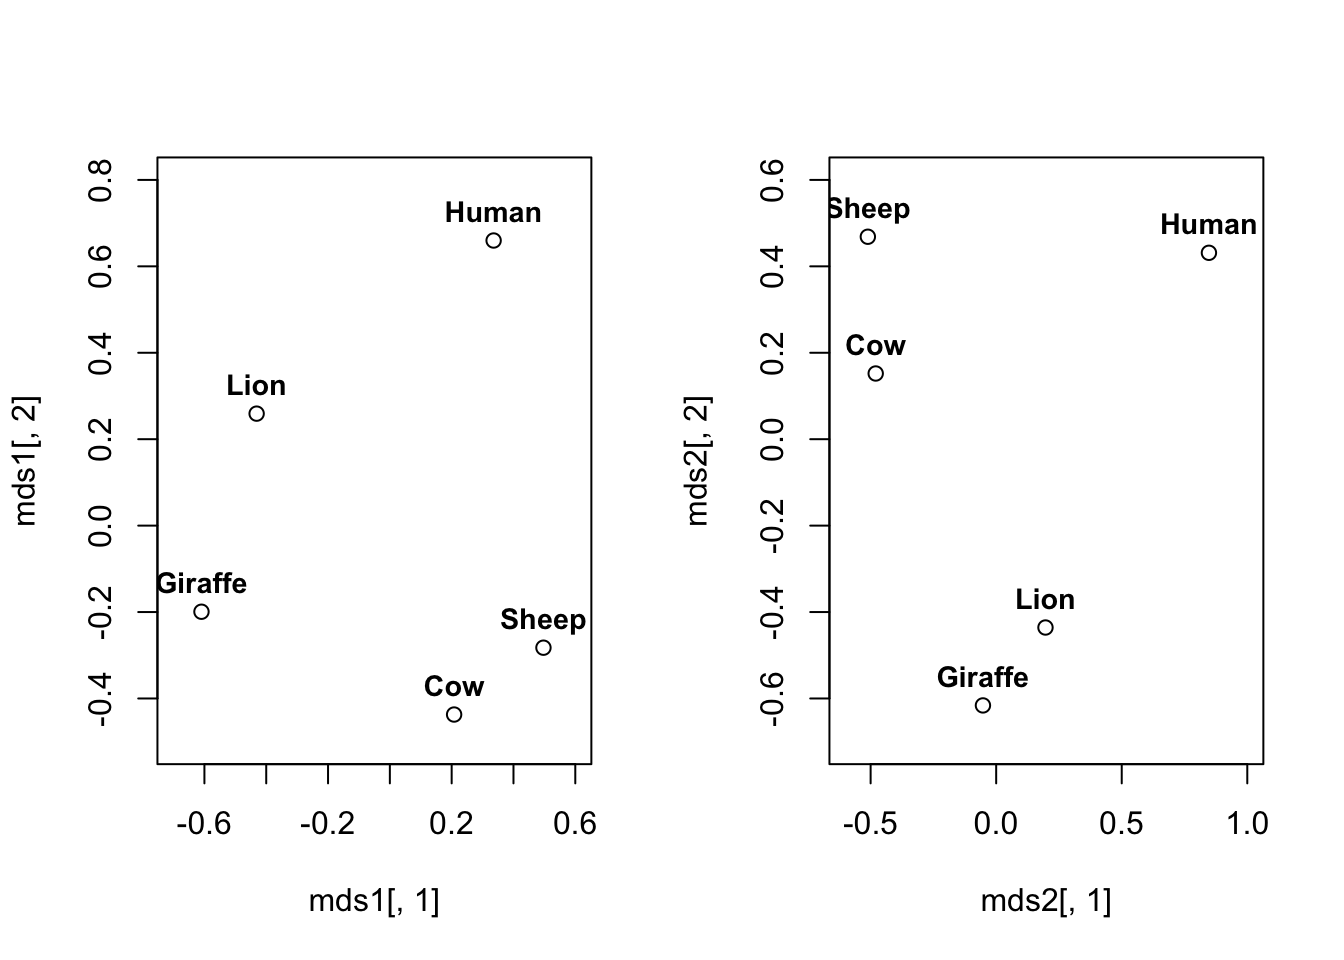
\includegraphics{06-mds_files/figure-latex/unnamed-chunk-29-1.pdf}

\begin{Shaded}
\begin{Highlighting}[]
\FunctionTok{ggplot}\NormalTok{(mds2, }\FunctionTok{aes}\NormalTok{(}\AttributeTok{x=}\NormalTok{X1, }\AttributeTok{y=}\NormalTok{X2, }\AttributeTok{colour=}\NormalTok{Digit, }\AttributeTok{label=}\NormalTok{Digit))}\SpecialCharTok{+}
  \FunctionTok{geom\_text}\NormalTok{(}\FunctionTok{aes}\NormalTok{(}\AttributeTok{label=}\NormalTok{Digit))}\SpecialCharTok{+} 
  \FunctionTok{ggtitle}\NormalTok{(}\StringTok{"MDS for MNIST using the Jaccard index"}\NormalTok{) }
\end{Highlighting}
\end{Shaded}

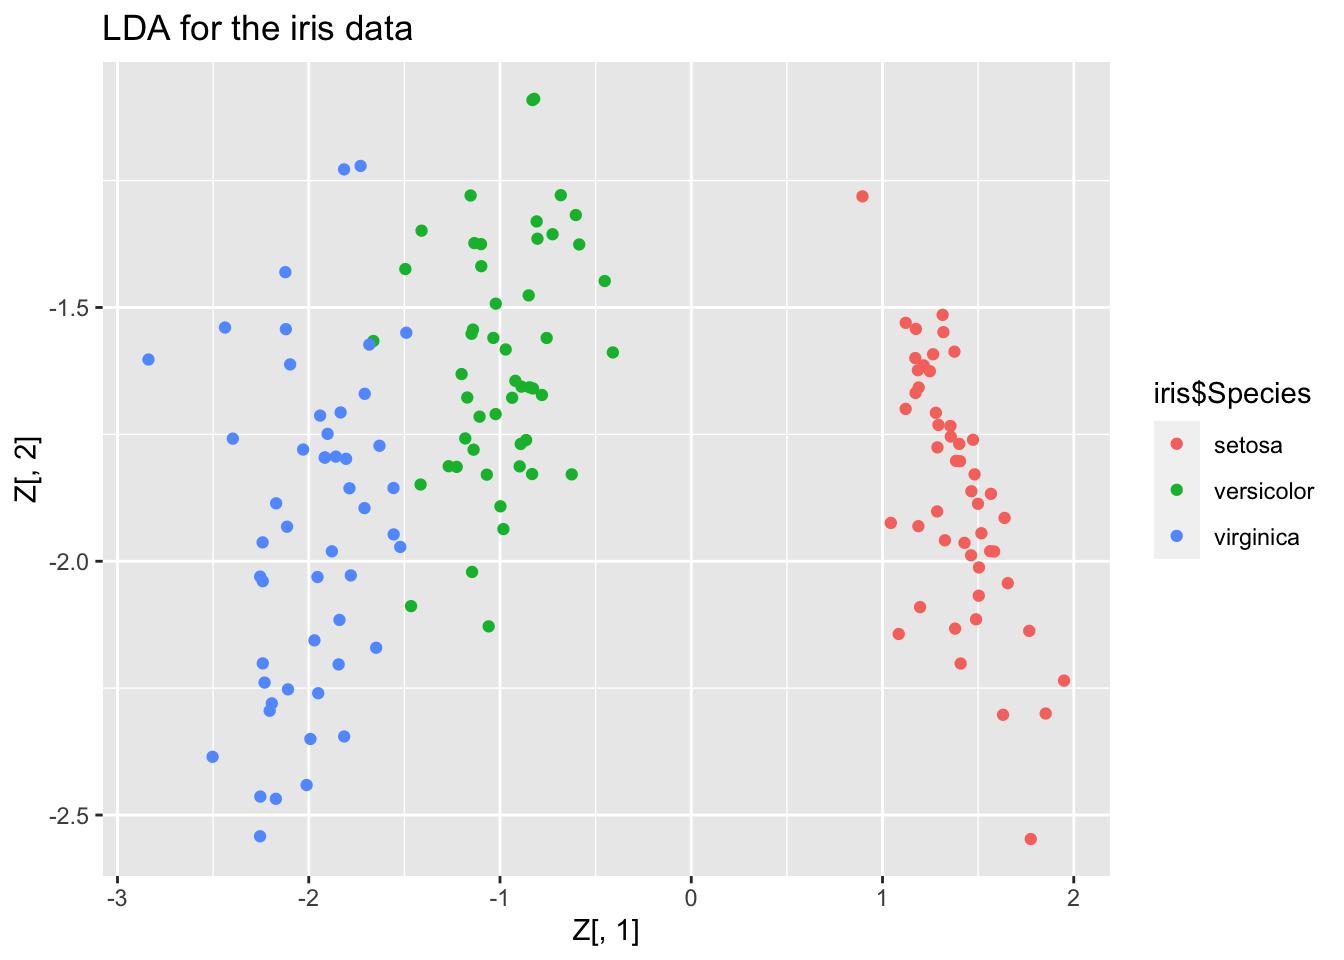
\includegraphics{06-mds_files/figure-latex/unnamed-chunk-29-2.pdf}

You can see that we get two different representations of the data that differ from each other, and from the PCA representation we computed in Chapter \ref{pca}.

\section{Non-metric MDS}\label{non-metric-mds}

In this chapter we have focused on classical MDS, which looks for points that have \textbf{Euclidean} distances close to the desired distances, where we measured close by minimizing the sum of squared errors (cf Equation \eqref{eq:mdsopt}).

There is a much wider class of multidimensional scaling methods that do not use Euclidean distances, and do not judge the approximation quality using squared errors. These MDS methods can sometimes produce sets of coordinates that are more useful than classical MDS. However, it is only for classical MDS that there is a closed form solution. More general MDS methods rely upon numerical optimization to find a solution to the optimization problem. If you are interested, take a look at the R commands \texttt{isoMDS}, \texttt{Shepard}, and \texttt{sammon} from the \texttt{MASS} R package. Sammon mapping, for example, puts a greater emphasis on preserving smaller distances.

More generally still, there has been a lot of work on non-linear dimension reduction methods that try to find a low dimensional manifold upon which the data lie. Have a look \href{https://colah.github.io/posts/2014-10-Visualizing-MNIST/}{here} for some amazing visualizations and results using the MNIST dataset. These methods are not always easy to work with, and can require detailed user supervision in order to work well.

\section{Exercises}\label{exercises-3}

\begin{enumerate}
\def\labelenumi{\arabic{enumi}.}
\item
  In this question we will prove part 1. Theorem \ref{thm:five1}.

  \begin{enumerate}
  \def\labelenumii{\roman{enumii}.}
  \item
    Define
    \[
    b_{ij}=(\mathbf x_i-\bar{\mathbf x})^\top (\mathbf x_j-\bar{\mathbf x}), \quad i,j=1, \ldots , n,
    \]
    and write \(\mathbf B=(b_{ij})_{i,j=1}^n\). Prove that \[\mathbf B=(\mathbf H\mathbf X)(\mathbf H\mathbf X)^\top,\] where
    \(\mathbf H\) is the \(n \times n\) centering matrix and \(\mathbf X= (\mathbf x_1, \ldots , \mathbf x_n)^\top\) is the data matrix.
  \item
    Show that \(\mathbf B\) is positive semi-definite, i.e., explain why, for
    all \(n \times 1\) vectors \(\mathbf a\),
    \[
    \mathbf a^\top \mathbf B\mathbf a=\mathbf a^\top (\mathbf H\mathbf X) (\mathbf H\mathbf X)^\top \mathbf a\geq 0. 
    \]
  \end{enumerate}
\item
  In this question we will prove part 2. of Theorem \ref{thm:five1}

  \begin{enumerate}
  \def\labelenumii{\roman{enumii}.}
  \item
    Prove Property 7. of Section \ref{centering-matrix}. Specifically: if \(\mathbf A\) is a symmetric \(n \times n\) matrix, show that
    \[\mathbf B= \mathbf H\mathbf A\mathbf H\]
    has elements given by
    \[
    b_{ij}=a_{ij}-\bar{a}_{i+}-\bar{a}_{+j}+\bar{a}_{++},  \qquad i,j=1, \ldots , n,
    \]
    where\\
    \[\bar{a}_{i+}= \frac{1}{n} \sum_{j=1}^n a_{ij}, \quad \bar{a}_{+j}=\frac{1}{n} \sum_{i=1}^n a_{ij}, \quad\mbox{and} \quad\bar{a}_{++} = \frac{1}{n^2} \sum_{i,j=1}^n a_{ij}.\]
  \item
    Assume that \(\mathbf B\) is positive semi-definite with \(k\) strictly positive eigenvalues and let
    \[
    \mathbf B= \sum_{j=1}^k \lambda_j \mathbf u_j\mathbf u_j^\top =\mathbf U\boldsymbol \Lambda\mathbf U^\top,
    \]
    where \(\boldsymbol \Lambda=\text{diag}\{\lambda_1, \ldots , \lambda_k\}\) and \(\mathbf U\) is \(n \times k\) and satisfies \(\mathbf U^\top \mathbf U=\mathbf I_k\).
    Now define a `new' \(n \times k\) data matrix
    \[
    \mathbf X=[\mathbf x_1, \ldots , \mathbf x_n]^\top=\mathbf U\boldsymbol \Lambda^{1/2}.
    \]
    Show that \(b_{ij}=\mathbf x_i^\top \mathbf x_j\) for all \(i,j=1, \ldots , n\).\\
    \textbf{Hint}: check that for \(\mathbf X\) defined as above, \(\mathbf X\mathbf X^\top =\mathbf B\).
  \item
    We now need to show that \(\mathbf D=(d_{ij})\) represents the set of inter-point distances for this new data matrix. Recall that \(a_{ij}=-d_{ij}^2/2\). Deduce that
    \[
    (\mathbf x_i -\mathbf x_j)^\top (\mathbf x_i-\mathbf x_j)= b_{ii} + b_{jj}-2b_{ij};
    \]
    and so, using the first part of this question, show that
    \[
    (\mathbf x_i -\mathbf x_j)^\top (\mathbf x_i-\mathbf x_j)=-2a_{ij}=d_{ij}^2.
    \]
    Hence the new inter-point distances are the same as the original ones.
  \end{enumerate}
\item
  Suppose \(\mathbf X\) is a \(n \times p\) column centred data matrix. PCA looks at the spectral decomposition of the covariance matrix \(\frac{1}{n}\mathbf X^\top \mathbf X\), whereas MDS uses the spectral decomposition of the Gram matrix \(\mathbf X\mathbf X^\top\). Using the SVD for \(\mathbf X=\mathbf U\boldsymbol{\Sigma}\mathbf V^\top\), explain the relationship between these two methods.
\end{enumerate}

\begin{enumerate}
\def\labelenumi{\arabic{enumi}.}
\setcounter{enumi}{3}
\tightlist
\item
  Answer Q4 part (c) from the 2018-19 exam paper.
\end{enumerate}

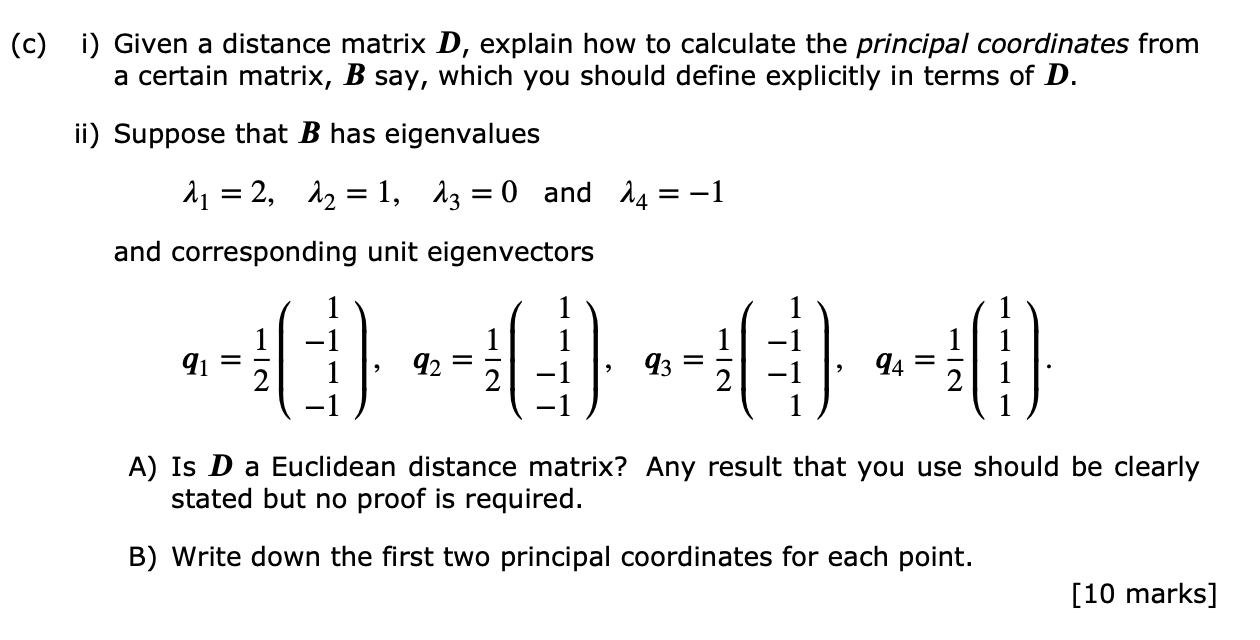
\includegraphics{figs/MDS_2018_19_Q4.png}

\begin{enumerate}
\def\labelenumi{\arabic{enumi}.}
\setcounter{enumi}{4}
\tightlist
\item
  Answer Q4 part (a) from the 2017-18 exam paper. Here, the `similarity matching coefficient' is what we called the \emph{simple matching coefficient} (SMC) in the notes.
\end{enumerate}

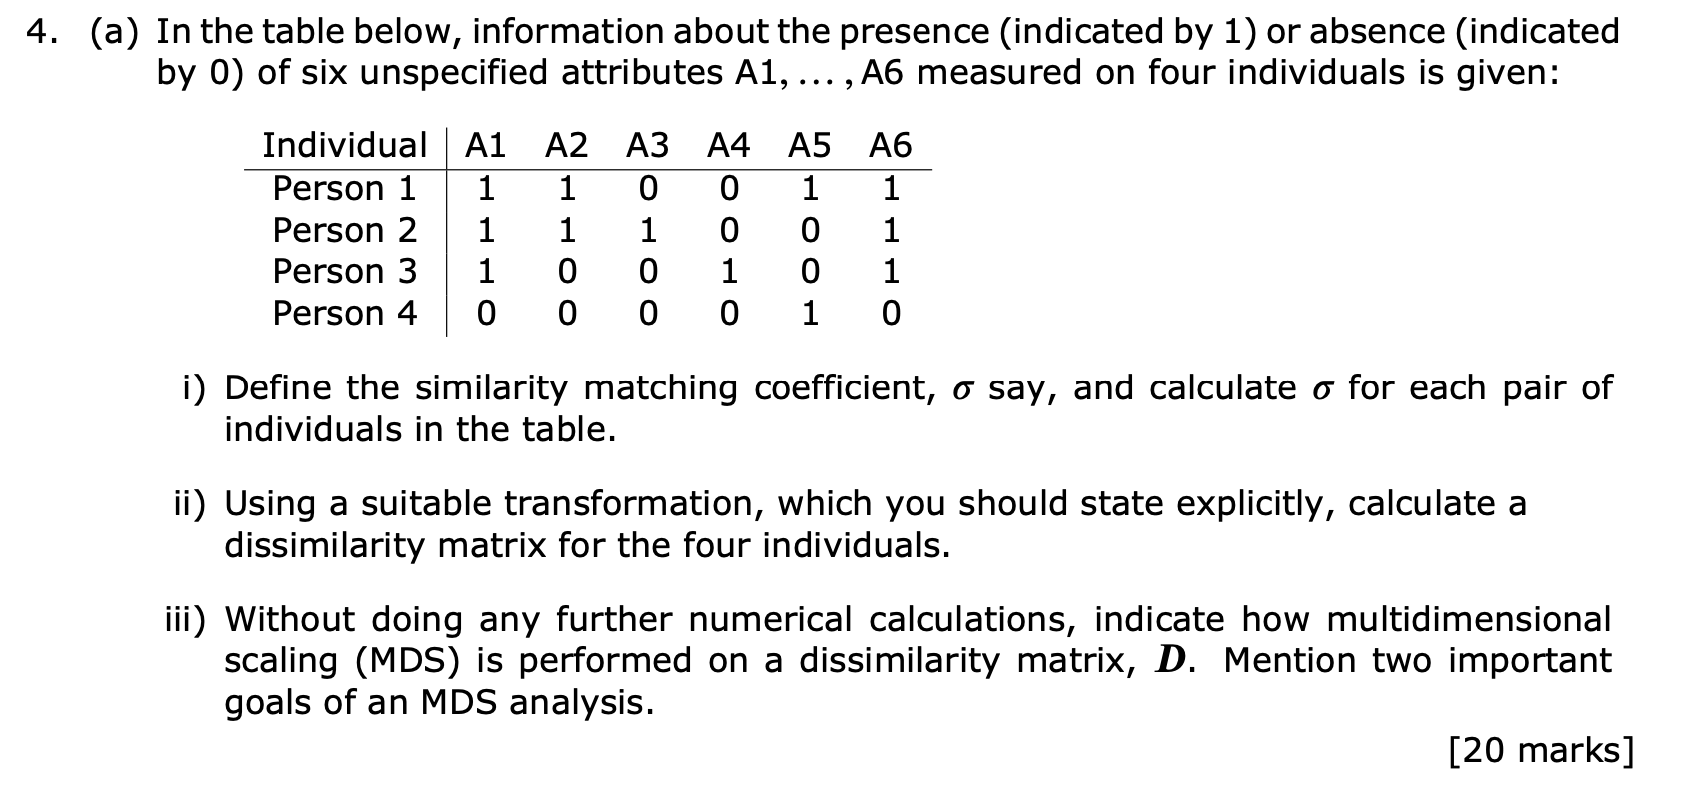
\includegraphics{figs/MDS_2017_18_Q4.png}

\section{Computer Tasks}\label{computer-tasks-2}

\paragraph*{Task 1}\label{task-1-1}
\addcontentsline{toc}{paragraph}{Task 1}

The \texttt{eurodist} dataset in R gives the road distances between 21 European cities. Note that this is stored as a \texttt{dist} type of object, as outputted by the \texttt{dist} command, i.e.~as a lower tri-diagonal matrix. \texttt{cmdscale} will take this directly as input.

\begin{Shaded}
\begin{Highlighting}[]
\FunctionTok{data}\NormalTok{(eurodist)}
\NormalTok{eurodist}
\NormalTok{?eurodist}
\end{Highlighting}
\end{Shaded}

\begin{enumerate}
\def\labelenumi{\roman{enumi}.}
\item
  Perform multidimensional scaling on this data, and find a two-dimensional set of points which has interpoint distances approximately equal to the data.
\item
  Plot these coordinates and label them with the city names. Does your plot look like the map of Europe?
\item
  Is the distance matrix \texttt{eurodist} a Euclidean data matrix and how do you know? If it is not Euclidean, why do you think that might be?
\item
  Create the Euclidean distance matrix from your set of 2-dimensional points. What is the Frobenius norm between this matrix and the original distance matrix? Use \texttt{cmdscale} to create a set of points in 3 dimensional space and recompute the distance matrix.
\end{enumerate}

\paragraph*{Task 2}\label{task-2-1}
\addcontentsline{toc}{paragraph}{Task 2}

Consider the synthetic data of 9 binary attributes on 11 cases.

\begin{Shaded}
\begin{Highlighting}[]
\NormalTok{df}\OtherTok{=}\FunctionTok{structure}\NormalTok{(}\FunctionTok{list}\NormalTok{(}\AttributeTok{a =} \FunctionTok{c}\NormalTok{(}\DecValTok{0}\NormalTok{, }\DecValTok{0}\NormalTok{, }\DecValTok{0}\NormalTok{, }\DecValTok{0}\NormalTok{, }\DecValTok{1}\NormalTok{, }\DecValTok{0}\NormalTok{, }\DecValTok{0}\NormalTok{, }\DecValTok{1}\NormalTok{, }\DecValTok{0}\NormalTok{, }\DecValTok{0}\NormalTok{, }\DecValTok{0}\NormalTok{), }\AttributeTok{b =} \FunctionTok{c}\NormalTok{(}\DecValTok{0}\NormalTok{, }
\DecValTok{0}\NormalTok{, }\DecValTok{0}\NormalTok{, }\DecValTok{0}\NormalTok{, }\DecValTok{0}\NormalTok{, }\DecValTok{0}\NormalTok{, }\DecValTok{1}\NormalTok{, }\DecValTok{0}\NormalTok{, }\DecValTok{1}\NormalTok{, }\DecValTok{0}\NormalTok{, }\DecValTok{1}\NormalTok{), }\AttributeTok{c =} \FunctionTok{c}\NormalTok{(}\DecValTok{0}\NormalTok{, }\DecValTok{0}\NormalTok{, }\DecValTok{0}\NormalTok{, }\DecValTok{0}\NormalTok{, }\DecValTok{1}\NormalTok{, }\DecValTok{0}\NormalTok{, }\DecValTok{0}\NormalTok{, }\DecValTok{1}\NormalTok{, }
\DecValTok{0}\NormalTok{, }\DecValTok{1}\NormalTok{, }\DecValTok{0}\NormalTok{), }\AttributeTok{d =} \FunctionTok{c}\NormalTok{(}\DecValTok{1}\NormalTok{, }\DecValTok{0}\NormalTok{, }\DecValTok{0}\NormalTok{, }\DecValTok{0}\NormalTok{, }\DecValTok{0}\NormalTok{, }\DecValTok{0}\NormalTok{, }\DecValTok{1}\NormalTok{, }\DecValTok{0}\NormalTok{, }\DecValTok{0}\NormalTok{, }\DecValTok{1}\NormalTok{, }\DecValTok{0}\NormalTok{), }\AttributeTok{e =} \FunctionTok{c}\NormalTok{(}\DecValTok{0}\NormalTok{, }\DecValTok{0}\NormalTok{, }
\DecValTok{1}\NormalTok{, }\DecValTok{0}\NormalTok{, }\DecValTok{0}\NormalTok{, }\DecValTok{0}\NormalTok{, }\DecValTok{0}\NormalTok{, }\DecValTok{0}\NormalTok{, }\DecValTok{0}\NormalTok{, }\DecValTok{0}\NormalTok{, }\DecValTok{1}\NormalTok{), }\AttributeTok{f =} \FunctionTok{c}\NormalTok{(}\DecValTok{0}\NormalTok{, }\DecValTok{0}\NormalTok{, }\DecValTok{1}\NormalTok{, }\DecValTok{0}\NormalTok{, }\DecValTok{0}\NormalTok{, }\DecValTok{0}\NormalTok{, }\DecValTok{0}\NormalTok{, }\DecValTok{0}\NormalTok{, }\DecValTok{0}\NormalTok{, }
\DecValTok{0}\NormalTok{, }\DecValTok{1}\NormalTok{), }\AttributeTok{g =} \FunctionTok{c}\NormalTok{(}\DecValTok{0}\NormalTok{, }\DecValTok{1}\NormalTok{, }\DecValTok{1}\NormalTok{, }\DecValTok{1}\NormalTok{, }\DecValTok{0}\NormalTok{, }\DecValTok{0}\NormalTok{, }\DecValTok{0}\NormalTok{, }\DecValTok{0}\NormalTok{, }\DecValTok{0}\NormalTok{, }\DecValTok{0}\NormalTok{, }\DecValTok{0}\NormalTok{), }\AttributeTok{h =} \FunctionTok{c}\NormalTok{(}\DecValTok{1}\NormalTok{, }\DecValTok{0}\NormalTok{, }\DecValTok{0}\NormalTok{, }
\DecValTok{0}\NormalTok{, }\DecValTok{0}\NormalTok{, }\DecValTok{0}\NormalTok{, }\DecValTok{0}\NormalTok{, }\DecValTok{1}\NormalTok{, }\DecValTok{1}\NormalTok{, }\DecValTok{0}\NormalTok{, }\DecValTok{0}\NormalTok{), }\AttributeTok{i =} \FunctionTok{c}\NormalTok{(}\DecValTok{0}\NormalTok{, }\DecValTok{0}\NormalTok{, }\DecValTok{0}\NormalTok{, }\DecValTok{0}\NormalTok{, }\DecValTok{0}\NormalTok{, }\DecValTok{1}\NormalTok{, }\DecValTok{0}\NormalTok{, }\DecValTok{0}\NormalTok{, }\DecValTok{1}\NormalTok{, }\DecValTok{1}\NormalTok{, }
\DecValTok{0}\NormalTok{)), }\AttributeTok{class =} \StringTok{"data.frame"}\NormalTok{, }\AttributeTok{row.names =} \FunctionTok{c}\NormalTok{(}\ConstantTok{NA}\NormalTok{, }\SpecialCharTok{{-}}\DecValTok{11}\DataTypeTok{L}\NormalTok{), }\AttributeTok{.Names =} \FunctionTok{c}\NormalTok{(}\StringTok{"a"}\NormalTok{, }
\StringTok{"b"}\NormalTok{, }\StringTok{"c"}\NormalTok{, }\StringTok{"d"}\NormalTok{, }\StringTok{"e"}\NormalTok{, }\StringTok{"f"}\NormalTok{, }\StringTok{"g"}\NormalTok{, }\StringTok{"h"}\NormalTok{, }\StringTok{"i"}\NormalTok{))}
\NormalTok{df}
\end{Highlighting}
\end{Shaded}

\begin{verbatim}
##    a b c d e f g h i
## 1  0 0 0 1 0 0 0 1 0
## 2  0 0 0 0 0 0 1 0 0
## 3  0 0 0 0 1 1 1 0 0
## 4  0 0 0 0 0 0 1 0 0
## 5  1 0 1 0 0 0 0 0 0
## 6  0 0 0 0 0 0 0 0 1
## 7  0 1 0 1 0 0 0 0 0
## 8  1 0 1 0 0 0 0 1 0
## 9  0 1 0 0 0 0 0 1 1
## 10 0 0 1 1 0 0 0 0 1
## 11 0 1 0 0 1 1 0 0 0
\end{verbatim}

\begin{enumerate}
\def\labelenumi{\roman{enumi}.}
\item
  Compute the Jaccard index and SMC similarity matrices for these data.
\item
  Perform classical MDS for both similarity matrices, producing a plot of the coordinates (in 2d). Are the results similar?
\end{enumerate}

\paragraph*{Task 3}\label{task-3-1}
\addcontentsline{toc}{paragraph}{Task 3}

In this question we will look at data from 1888 on the fertility and socio-economic status of 47 French speaking provinces in Switzerland.

\begin{Shaded}
\begin{Highlighting}[]
\FunctionTok{data}\NormalTok{(swiss)}
\FunctionTok{head}\NormalTok{(swiss)}
\end{Highlighting}
\end{Shaded}

\begin{verbatim}
##              Fertility Agriculture Examination Education Catholic
## Courtelary        80.2        17.0          15        12     9.96
## Delemont          83.1        45.1           6         9    84.84
## Franches-Mnt      92.5        39.7           5         5    93.40
## Moutier           85.8        36.5          12         7    33.77
## Neuveville        76.9        43.5          17        15     5.16
## Porrentruy        76.1        35.3           9         7    90.57
##              Infant.Mortality
## Courtelary               22.2
## Delemont                 22.2
## Franches-Mnt             20.2
## Moutier                  20.3
## Neuveville               20.6
## Porrentruy               26.6
\end{verbatim}

\begin{Shaded}
\begin{Highlighting}[]
\NormalTok{?swiss}
\end{Highlighting}
\end{Shaded}

We will use MDS to find which provinces are similar to each other.

\begin{enumerate}
\def\labelenumi{\roman{enumi}.}
\item
  Compute the Euclidean distance matrix for these data.
\item
  Use MDS to create a 2-dimensional representation of the data and plot these points, labelling them with the province name.
\item
  Use MDS to create a 3-dimensional representation of the data. You can plot this using the \texttt{plot3d} command from the \texttt{rgl} package. See, for example, \href{https://rpubs.com/aagarwal29/179912}{here}.
\end{enumerate}

\begin{Shaded}
\begin{Highlighting}[]
\FunctionTok{library}\NormalTok{(rgl)}
\FunctionTok{plot3d}\NormalTok{(mds3)}
\end{Highlighting}
\end{Shaded}

\begin{enumerate}
\def\labelenumi{\roman{enumi}.}
\setcounter{enumi}{2}
\tightlist
\item
  MDS can be also used to reveal a hidden pattern in a correlation matrix. Find the correlation matrix, \(\mathbf R\), of the swiss data. Perform MDS using \(1-\mathbf R\) as the distance matrix and plot the results. Positively correlated covariates are close together on the same side of the plot.
\end{enumerate}

\paragraph*{Task 4 (if you have time\ldots)}\label{task-4-if-you-have-time}
\addcontentsline{toc}{paragraph}{Task 4 (if you have time\ldots)}

Try MDS on the MNIST data but looking for a 3d representation. Colour the points by their digit label, and create some interactive 3d plots. Does this find useful structure in the data? And is it more informative than the 2d plots we created in the notes.

Read the description of more advance methods \href{https://colah.github.io/posts/2014-10-Visualizing-MNIST/}{here}. Pick one and find an R package that implements it and try it on the MNIST data.

\textbf{Warning:} The MNIST dataset is large, and so computations can take a long time if you use the full dataset. Thus I usually work with a selection of just 1000 images, which is enough to find interesting patterns in most cases.

\chapter*{Part III: Inference using the Multivariate Normal Distribution (MVN)}\label{part-iii-inference-using-the-multivariate-normal-distribution-mvn}
\addcontentsline{toc}{chapter}{Part III: Inference using the Multivariate Normal Distribution (MVN)}

Part III of this module covers statistical inference based on the multivariate normal (MVN) distribution.

Chapter \ref{multinormal} focuses on classical distribution theory relating to the MVN distribution, including the Wishart distribution, which is defined on the set of symmetric positive definite matrices and is a natural generalisation of the \(\chi^2\) distribution. Another important distribution related to the MVN distribution is the Hotelling \(T^2\) distribution, which is a multivariate analogue of the Student's \(t\)-distribution.
The Wishart and Hotelling \(T^2\) distributions then allow us to conduct hypothesis tests concerning vector means in \(1\)-sample and \(2\)-sample settings.

Chapter \ref{lm} is concerned with the multivariate linear model, in which the responses consist of random vectors rather than single random variables. Errors in this setting take the form of random vectors.

\chapter{The Multivariate Normal Distribution}\label{multinormal}

The multivariate normal distribution (MVN) generalises the univariate normal distribution from scalar to vector random variables. It is important for a number of reasons:

\begin{enumerate}
\def\labelenumi{\arabic{enumi}.}
\tightlist
\item
  It is entirely defined by its mean vector \({\boldsymbol{\mu}}\) and its covariance matrix \(\boldsymbol{\Sigma}\).
\item
  Zero correlation implies independence.
\item
  Linear functions of multivariate normal vectors are also multivariate normal vectors.
\item
  The multivariate version of the Central Limit Theorem means that it appears naturally throughout statistics.
\item
  It has simple geometric properties, and is easy to work with mathematically.
\end{enumerate}

In this chapter we'll define the MVN and look at some its properties. We'll then look at multivariate analogues of the t-test for comparing the mean of different populations. This will involve us defining two important the distributions:

\begin{itemize}
\item
  \textbf{Wishart} distribution which we can think of as the multivariate \(\chi^2\) distrbution, and which gives the distribution of sample covariance matrices.
\item
  \textbf{Hotelling's \(T^2\)} distribution, which is the multivariate version of Student's t-distribution.
\end{itemize}

The videos for this chapter, in the order I recommend you watch, are available at

\begin{itemize}
\tightlist
\item
  \href{https://mediaspace.nottingham.ac.uk/media/Multivariate+Normal+Random+VariablesA+Introduction/1_pdjxphay}{7.1 Introduction to the multivariate normal distribution}
\item
  \href{https://mediaspace.nottingham.ac.uk/media/Multivariate+Normal+Random+VariablesA++Properties/1_j9mh4v7r}{7.1 Properties of the MVN distribution}
\item
  \href{https://mediaspace.nottingham.ac.uk/media/Multivariate+Normal+Random+VariablesA++Confidence+Ellipses/1_dlvgqoi3}{7.1.4 Confidence ellipses for the MVN}
\item
  \href{https://mediaspace.nottingham.ac.uk/media/MVN_HypothesistestIntro.mp4/1_b1gstf1h}{7.4 Introduction to hypothesis testing}
\item
  \href{https://mediaspace.nottingham.ac.uk/media/MVN_Wishart/1_3kpedgb6}{7.2 Wishart distribution}
\item
  \href{https://mediaspace.nottingham.ac.uk/media/MVN_WishartProperties/1_yfgzcsyb}{7.2.1 Properties of the Wishart distribution}
\item
  \href{https://mediaspace.nottingham.ac.uk/media/MVN_Hotelling.mp4/1_5evjeyu8}{7.3 Hotelling's \(T^2\) distribution}
\item
  \href{https://mediaspace.nottingham.ac.uk/media/Multivariate+NormalsA+Hypothesis+testing/1_bhk20k5z}{7.4 Hypothesis tests with Hotelling's \(T^2\) distribution}
\end{itemize}

\section{Definition and Properties of the MVN}\label{definition-and-properties-of-the-mvn}

\subsection{Basics}\label{basics}

\begin{definition}
\protect\hypertarget{def:mvn}{}\label{def:mvn}A random vector \(\mathbf x=(x_1, \ldots , x_p)^\top\) has a \(p\)-dimensional MVN distribution if and only if \(\mathbf a^\top \mathbf x\) is a univariate normal random variable for all constant vectors \(\mathbf a\in \mathbb{R}^p\).
\end{definition}

In particular, note that the marginal distribution of each element of \(\mathbf x\) has a uni-variate Gaussian distribution.

\textbf{Notation}: \quad If \(\mathbf x\in \mathbb{R}^p\) is MVN with mean \({\boldsymbol{\mu}}\in \mathbb{R}^p\) and covariance matrix \(\boldsymbol{\Sigma}\in \mathbb{R}^{p\times p}\) then we write
\[ \mathbf x\sim N_p ({\boldsymbol{\mu}}, \boldsymbol{\Sigma}).\]

\begin{definition}
\protect\hypertarget{def:mvnpdf}{}\label{def:mvnpdf}If the population covariance matrix \(\boldsymbol{\Sigma}\) (\(p \times p\)) is positive definite (i.e.~full rank), so that \(\boldsymbol{\Sigma}^{-1}\) exists,
then the \textbf{probability density function} (pdf) of the MVN distribution is given by
\[ f(\mathbf x) = \frac{1}{| 2 \pi \boldsymbol{\Sigma}|^{1/2}} \exp \left(-\frac{1}{2}(\mathbf x- {\boldsymbol{\mu}})^\top \boldsymbol{\Sigma}^{-1} (\mathbf x- {\boldsymbol{\mu}}) \right).\]
Here, I've used the notation \(|\mathbf A| = \det(\mathbf A)\).
\end{definition}

If \(p=1\), so that \(\mathbf x= x\), \({\boldsymbol{\mu}}= \mu\) and \(\boldsymbol{\Sigma}= \sigma^2\), say, then the pdf simplifies to
\begin{eqnarray*}
f(\mathbf x) &=& \frac{1}{|2 \pi \sigma^2|^{1/2}} \exp \left(-\frac{1}{2}(x - \mu) (\sigma^2)^{-1} (x - \mu) \right)\\
&=& \frac{1}{(2 \pi \sigma^2)^{1/2}} \exp \left(-\frac{1}{2 \sigma^2}(x - \mu)^2 \right)
\end{eqnarray*}
which is the familiar pdf of the univariate normal distribution \(N(\mu,\sigma^2)\).

If \(p>1\) and \(\boldsymbol{\Sigma}= \operatorname{diag}(\sigma_1^2, \ldots, \sigma_p^2)\) then
\begin{eqnarray*}
f(\mathbf x) &=& \frac{1}{((2 \pi)^{p}\prod_{i=1}^p \sigma_i^2)^{1/2}} \exp \left(-\frac{1}{2}(\mathbf x- {\boldsymbol{\mu}})^\top \boldsymbol{\Sigma}^{-1}(\mathbf x- {\boldsymbol{\mu}}) \right)\\
&=& \frac{1}{(2 \pi)^{p/2}\prod_{i=1}^p \sigma_i} \exp \left(-\frac{1}{2} \sum_{i=1}^p \frac{(x_i - \mu_i)^2}{\sigma_i^2} \right)\\
&=& \left(\frac{1}{\sqrt{2 \pi\sigma_1^2}} \exp \left(-\frac{1}{2\sigma_1^2} (x_1 - \mu_1)^2 \right)\right)\\
 && \qquad \qquad \times \ldots \left(\frac{1}{\sqrt{2 \pi \sigma_p^2}} \exp \left(-\frac{1}{2\sigma_p^2} (x_p - \mu_p)^2 \right)\right)
\end{eqnarray*}
Thus, by the factorisation theorem for probability densities, the components of \(\mathbf x\) have independent univariate normal distributions: \(x_i \sim N(\mu_i, \sigma_i^2)\).

If \(p=2\) we can plot \(f(\mathbf x)\) using contour plots. Below, I've generated 1000 points from four different normal distributions using mean vectors
\[{\boldsymbol{\mu}}_1={\boldsymbol{\mu}}_3={\boldsymbol{\mu}}_4=\begin{pmatrix}0 \\0 \\\end{pmatrix}, \quad {\boldsymbol{\mu}}_2=\begin{pmatrix}1 \\-1 \\\end{pmatrix}\]
and covariance matrices
\[\boldsymbol{\Sigma}_1=\boldsymbol{\Sigma}_2=\begin{pmatrix}1&0 \\0&1 \\\end{pmatrix}, \quad \boldsymbol{\Sigma}_3=\begin{pmatrix}1&0 \\0&0.05 \\\end{pmatrix}, \quad \boldsymbol{\Sigma}_4=\begin{pmatrix}1&0.9 \\0.9&1 \\\end{pmatrix}.\]

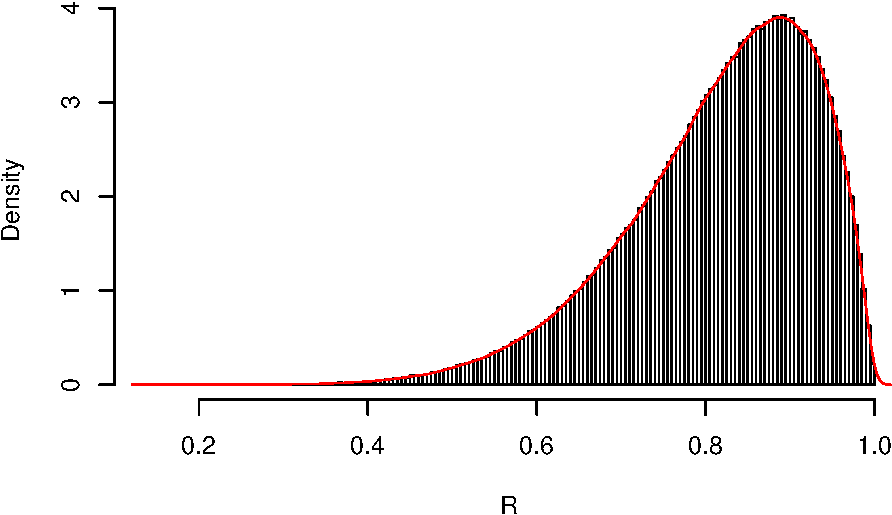
\includegraphics{07-mvn_files/figure-latex/unnamed-chunk-3-1.pdf}

\textbf{Note} that the top left and bottom right plots have the \textbf{same marginal distribtions} for components \(x_1\) and \(x_2\), namely
\[x_1 \sim N(0, 1)\quad x_2 \sim N(0, 1)\]

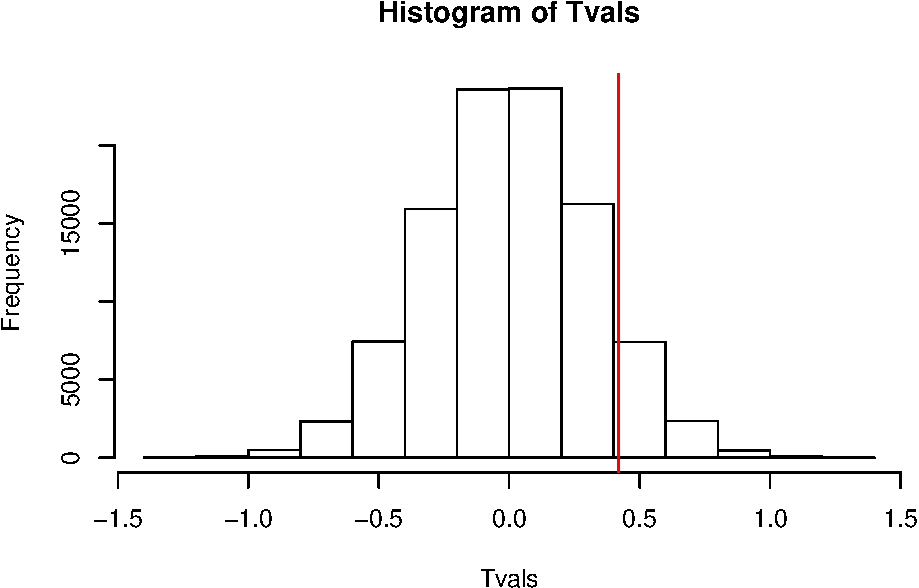
\includegraphics{07-mvn_files/figure-latex/unnamed-chunk-4-1.pdf} \includegraphics{07-mvn_files/figure-latex/unnamed-chunk-4-2.pdf}

The contours on each plot are obtained by finding values of \(\mathbf x\) for which \(f(\mathbf x)=c\). The constant \(c\) is chosen so that the the shapes (which we'll see below are ellipses)
enclose 66\% and 95\% of the data.

\subsection{Transformations}\label{transformations}

\begin{proposition}
\protect\hypertarget{prp:six2}{}\label{prp:six2}If \(\mathbf x\sim N_p({\boldsymbol{\mu}},\boldsymbol{\Sigma})\) then if \[\mathbf y= \mathbf A\mathbf x+ \mathbf c, \mbox{ where } \mathbf A\in \mathbb{R}^{q \times p} \mbox{ and }\mathbf c\in \mathbb{R}^q
  \mbox{ are constant},\] then
\[\mathbf y\sim N_q(\mathbf A{\boldsymbol{\mu}}+ \mathbf c, \mathbf A\boldsymbol{\Sigma}\mathbf A^\top).\]
\end{proposition}

\begin{proof}
Let \(\mathbf b\in \mathbb{R}^q\) be a constant vector. Then
\[ \mathbf b^\top \mathbf y= \mathbf b^\top \mathbf A\mathbf x+ \mathbf b^\top \mathbf c= \mathbf a^\top \mathbf x+ \mathbf b^\top \mathbf c\]
where \(\mathbf a^\top = \mathbf b^\top \mathbf A\). Now \(\mathbf a^\top \mathbf x\) is univariate normal for all \(\mathbf a\) since \(\mathbf x\) is MVN. Therefore \(\mathbf b^\top \mathbf y\) is univariate normal for all \(\mathbf b\), so \(\mathbf y\) is MVN.

We can compute \({\mathbb{E}}(\mathbf y)=\mathbf A{\boldsymbol{\mu}}+\mathbf c\) and \({\mathbb{V}\operatorname{ar}}(\mathbf y)=\mathbf A\boldsymbol{\Sigma}\mathbf A^\top\) using the properties listed in Section \ref{randvec}.
\end{proof}

This implies that a linear transformation of a MVN random variable is also MVN. We can use this result to prove two important corollaries. The first corollary is useful for simulating data from a general MVN distribution.

\begin{corollary}
\protect\hypertarget{cor:csix2}{}\label{cor:csix2}If \(\mathbf x\sim N_p({\boldsymbol 0},\mathbf I_p)\) and \(\mathbf y= \boldsymbol{\Sigma}^{1/2} \mathbf x+ {\boldsymbol{\mu}}\) then \[\mathbf y\sim N_p({\boldsymbol{\mu}},\boldsymbol{\Sigma}).\]
\end{corollary}

\begin{proof}
Apply \ref{prp:six2} with \(\mathbf A= \boldsymbol{\Sigma}^{1/2}\) and \(\mathbf c= {\boldsymbol{\mu}}\). Therefore
\[{\mathbb{E}}(\mathbf y) = \boldsymbol{\Sigma}^{1/2} {\boldsymbol 0}_p + {\boldsymbol{\mu}}= {\boldsymbol{\mu}}\quad \mbox{and}\quad {\mathbb{V}\operatorname{ar}}(\mathbf y) = \boldsymbol{\Sigma}^{1/2} \mathbf I_p \boldsymbol{\Sigma}^{1/2} = \boldsymbol{\Sigma}.\]
\end{proof}

The second corollary says that any MVN random variable can be transformed into standard form.

\begin{corollary}
\protect\hypertarget{cor:csix3}{}\label{cor:csix3}Suppose \(\mathbf x\sim N_p({\boldsymbol{\mu}},\boldsymbol{\Sigma})\), where \(\boldsymbol{\Sigma}\) has full rank. Then\\
\[\mathbf y= \boldsymbol{\Sigma}^{-1/2}(\mathbf x- {\boldsymbol{\mu}}) \sim N_p({\boldsymbol 0},\mathbf I_p).\]
\end{corollary}

\begin{proof}
Apply Proposition \ref{prp:six2} with \(\mathbf A= \boldsymbol{\Sigma}^{-1/2}\) and \(\mathbf c= - \boldsymbol{\Sigma}^{-1/2} {\boldsymbol{\mu}}\).
\end{proof}

\subsection{Independence}\label{independence}

\begin{proposition}
\protect\hypertarget{prp:six4}{}\label{prp:six4}Two vectors \(\mathbf x\in\mathbb{R}^p\) and \(\mathbf y\in\mathbb{R}^q\) which are jointly multivariate normal are independent if and only if they are uncorrelated, i.e.~\({\mathbb{C}\operatorname{ov}}(\mathbf x,\mathbf y) = {\boldsymbol 0}_{p,q}\).
\end{proposition}

\begin{proof}
The joint distribution of \(\mathbf x\) and \(\mathbf y\) can always be factorized as
\[p(\mathbf x, \mathbf y)= p(\mathbf x)p(\mathbf y|\mathbf x).\]
If the conditional distribution for \(\mathbf y\) given \(\mathbf x\) does not depend upon \(\mathbf x\), i.e., if \(p(\mathbf y| \mathbf x)=p(\mathbf y)\), then \(\mathbf y\) and \(\mathbf x\) are independent.

Suppose \(\mathbf x\sim N_p({\boldsymbol{\mu}}_\mathbf x, \boldsymbol{\Sigma}_{\mathbf x,\mathbf x})\) and \(\mathbf y\sim N_p({\boldsymbol{\mu}}_\mathbf y, \boldsymbol{\Sigma}_{\mathbf y,\mathbf y})\) are jointly normally distributed and that they are uncorrelated. Thus we can write
\[\begin{pmatrix}\mathbf x\\ \mathbf y\end{pmatrix}\sim N_{p+q}\left({\boldsymbol{\mu}}, \boldsymbol{\Sigma}\right)
\]
where
\[{\boldsymbol{\mu}}= \begin{pmatrix}{\boldsymbol{\mu}}_\mathbf x\\ {\boldsymbol{\mu}}_{\mathbf y}\end{pmatrix}\quad \boldsymbol{\Sigma}= \begin{pmatrix} \boldsymbol{\Sigma}_{\mathbf x, \mathbf x} &{\boldsymbol 0}_{p,q}\\
{\boldsymbol 0}_{q,p} & \boldsymbol{\Sigma}_{\mathbf z, \mathbf z}\end{pmatrix}.\]

Now
\begin{align*}
p(\mathbf y|\mathbf x)&=\frac{p(\mathbf x, \mathbf y)}{p(\mathbf x)}\\
  &\propto \frac{\exp\left(-\frac{1}{2}(\mathbf x-{\boldsymbol{\mu}}_\mathbf x)^\top \boldsymbol{\Sigma}_{\mathbf x,\mathbf x}(\mathbf x-{\boldsymbol{\mu}}_\mathbf x) -\frac{1}{2}(\mathbf y-{\boldsymbol{\mu}}_\mathbf y)^\top \boldsymbol{\Sigma}_{\mathbf y,\mathbf y}(\mathbf y-{\boldsymbol{\mu}}_\mathbf y)\right)}{\exp\left(-\frac{1}{2}(\mathbf x-{\boldsymbol{\mu}}_\mathbf x)^\top \boldsymbol{\Sigma}_{\mathbf x,\mathbf x}(\mathbf x-{\boldsymbol{\mu}}_\mathbf x)\right)} \\
&\propto \exp\left(-\frac{1}{2}(\mathbf y-{\boldsymbol{\mu}}_\mathbf y)^\top \boldsymbol{\Sigma}_{\mathbf y,\mathbf y}(\mathbf y-{\boldsymbol{\mu}}_\mathbf y)\right) \\
&\propto p(\mathbf y)
\end{align*}
So \(p(\mathbf y|\mathbf x)=p(\mathbf y)\), i.e.~\(p(\mathbf y|\mathbf x)\) is not a function of \(\mathbf x\), and thus \(\mathbf x\) and \(\mathbf y\) are independent.
\end{proof}

Proposition \ref{prp:six4} means that zero correlation implies independence for the MVN distribution. This is not true in general for other distributions.

\textbf{Note:} It is important that \(\mathbf x\) and \(\mathbf y\) are \textbf{jointly} multivariate normal. For example, suppose \(x \sim N(0, 1)\). Let
\[z=\begin{cases}
1 \mbox{ with probability } \frac{1}{2}\\
-1 \mbox{ otherwise}
\end{cases}
\]
and let \(y=zx\). Then clearly \(y\) is also a normal random variable: \(y \sim N(0,1)\). In addition, note that
\[{\mathbb{C}\operatorname{ov}}(x,y)= {\mathbb{E}}(xy)= {\mathbb{E}}(x^2){\mathbb{E}}(z)=0\]
so that \(x\) and \(y\) are uncorrelated.

However, \(x\) and \(y\) are clearly not independent: if you tell me \(x\), then I know \(y=x\) or \(y=-x\).

\subsection{Confidence ellipses}\label{confidence-ellipses}

The contours in the plots of the bivariate normal samples shown above are ellipses.
They were defined to lines of consant density, i.e., by \(f(\mathbf x)=c\), which implies

\begin{equation}
(\mathbf x- {\boldsymbol{\mu}})^\top \boldsymbol{\Sigma}^{-1} (\mathbf x- {\boldsymbol{\mu}})=c' \label{eq:mvnellipse}
\end{equation}
for some constant \(c'\).
To see that this is the equation of an ellipse, note that a standard ellipse in \(\mathbb{R}^2\) is given by the equation
\begin{equation}
\frac{x^2}{a^2}+\frac{y^2}{b^2}=1 \quad (a, b>0) \label{eq:ellipse}
\end{equation}
and recall that a standard ellipse has axes of symmetry given by the \(x\)-axis and \(y\)-axis
(if \(a>b\), the \(x\)-axis is the major axis, and the \(y\)-axis the minor axis). For example, \(a=10, b=3\) gives the ellipse:

\includegraphics{07-mvn_files/figure-latex/unnamed-chunk-7-1.pdf}

If we define
\({\mathbf A}=\left(
\begin{array}{cc}
a^2&0\\
0&b^2
\end{array}
\right)\) and write \({\mathbf x}=\binom{x}{y}\),
then Equation \eqref{eq:ellipse} can be written in the form
\[ \mathbf x^\top {\mathbf A}^{-1}\mathbf x=c'. \]
To shift the centre of the ellipse from the origin to the point \({\boldsymbol{\mu}}\) we modify the equation to be
\[ (\mathbf x-{\boldsymbol{\mu}})^\top {\mathbf A}^{-1}(\mathbf x-{\boldsymbol{\mu}}) =c'.\]

What if instead of using a diagonal matrix \(\mathbf A\), we use a non-diagonal matrix \(\boldsymbol{\Sigma}\) as in Equation \eqref{eq:mvnellipse}? If \(\boldsymbol{\Sigma}\) has spectral decomposition
\(\boldsymbol{\Sigma}= \mathbf V\boldsymbol \Lambda\mathbf V^\top\), then
\begin{align*}
(\mathbf x-{\boldsymbol{\mu}})^\top {\boldsymbol{\Sigma}}^{-1}(\mathbf x-{\boldsymbol{\mu}}) &= (\mathbf x-{\boldsymbol{\mu}})^\top \mathbf V\boldsymbol \Lambda^{-1}\mathbf V^\top(\mathbf x-{\boldsymbol{\mu}}) \\
&= \mathbf y^\top \boldsymbol \Lambda^{-1}\mathbf y\\
&= \frac{y_1^2}{\lambda_1}+\frac{y_2^2}{\lambda_2}
\end{align*}
where \(\boldsymbol \Lambda=\operatorname{diag}(\lambda_1, \lambda_2)\) is a diagonal matrix of eigenvalues, and \(\mathbf y= \mathbf V^\top (\mathbf x-\mathbf u)\). Because \(\mathbf V\) is an orthogonal matrix (a rotation), we can see that this is the equation of a standard ellipse when using the eigenvectors as the coordinate system. Or in other words, it is an ellipse
with major axis given by the first eigenvector, and minor axis given by the second eigenvector, centered around \({\boldsymbol{\mu}}\).

Analogous results for ellipsoids and quadratic forms hold in three and higher dimensions.

The term \((\mathbf x-{\boldsymbol{\mu}})^\top \boldsymbol{\Sigma}^{-1} (\mathbf x-{\boldsymbol{\mu}})\)
will be important later in the chapter. The following proposition gives its distribution:

\begin{proposition}
\protect\hypertarget{prp:six5}{}\label{prp:six5}If \(\mathbf x\sim N_p({\boldsymbol{\mu}}, \boldsymbol{\Sigma})\) and \(\boldsymbol{\Sigma}\) is positive definite then
\[(\mathbf x-{\boldsymbol{\mu}})^\top \boldsymbol{\Sigma}^{-1} (\mathbf x-{\boldsymbol{\mu}}) \sim \chi_p^2.\]
\end{proposition}

\begin{proof}
Define \(\mathbf y= \boldsymbol{\Sigma}^{-1/2} (\mathbf x-{\boldsymbol{\mu}})\) so
\begin{align*}
(\mathbf x-{\boldsymbol{\mu}})^\top \boldsymbol{\Sigma}^{-1} (\mathbf x-{\boldsymbol{\mu}}) &= \left(\boldsymbol{\Sigma}^{-1/2} (\mathbf x-{\boldsymbol{\mu}}) \right)^\top \left(\boldsymbol{\Sigma}^{-1/2} (\mathbf x-{\boldsymbol{\mu}}) \right)\\
&= \mathbf y^\top \mathbf y= \sum_{i=1}^p y_i^2
\end{align*}
By Corollary \ref{cor:csix3}, \(\mathbf y\sim N_p ({\boldsymbol 0}, \mathbf I_p)\), and so the components of \(\mathbf y\) have independent univariate normal distributions with mean 0 and variance 1. Recall from univariate statistics that if \(z \sim N(0,1)\) then \(z^2 \sim \chi^2_1\) and if \(z_1, \ldots, z_n\) are iid \(N(0,1)\) then \(\sum_{i=1}^n z_i^2 \sim \chi_n^2\). It therefore follows that \[\sum_{i=1}^p y_i^2 \sim \chi^2_p.\]
\end{proof}

Proposition \ref{prp:six5} means we can calculate the probability \[{\mathbb{P}}\left((\mathbf x-{\boldsymbol{\mu}})^\top \boldsymbol{\Sigma}^{-1} (\mathbf x-{\boldsymbol{\mu}})<k\right),\] which is the probability of \(\mathbf x\) lying within a particular ellipsoid. We often use this to draw confidence ellipses, which are ellipses that we expect to contain some specified proportion of the random samples (95\% say).

\subsection{Sampling results for the MVN}\label{sampling-results-for-the-mvn}

In this section we present two important results which are natural
generalisations of what happens in the univariate case.

\begin{proposition}
\protect\hypertarget{prp:six6}{}\label{prp:six6}If \(\mathbf x_1, \ldots, \mathbf x_n\) is an IID random sample from \(N_p({\boldsymbol{\mu}}, \boldsymbol{\Sigma})\), then the sample mean and sample variance matrix
\[\bar{\mathbf x} = \frac{1}{n} \sum_{i=1}^n \mathbf x_i, \quad \mathbf S= \frac{1}{n} \sum_{i=1}^n (\mathbf x_i - \bar{\mathbf x})(\mathbf x_i-\bar{\mathbf x})^\top\] are independent.
\end{proposition}

\begin{proof}
From Proposition \ref{prp:six2} we can see that if \(\mathbf x_1, \ldots, \mathbf x_n \sim N_p({\boldsymbol{\mu}}, \boldsymbol{\Sigma})\) then \(\bar{\mathbf x} \sim N_p ({\boldsymbol{\mu}}, n^{-1}\boldsymbol{\Sigma})\). Let \(\mathbf y_i = \mathbf x_i -\bar{\mathbf x}\). Then
\begin{align*}
{\mathbb{C}\operatorname{ov}}(\bar{\mathbf x},\mathbf y_i)&={\mathbb{C}\operatorname{ov}}(\bar{\mathbf x}, \mathbf x_i -\bar{\mathbf x})\\
&={\mathbb{C}\operatorname{ov}}(\bar{\mathbf x}, \mathbf x_i) - {\mathbb{C}\operatorname{ov}}(\bar{\mathbf x}, \bar{\mathbf x})\\
&=n^{-1}\sum_{j=1}^n \left \{{\mathbb{E}}[(\mathbf x_j -{\boldsymbol{\mu}})(\mathbf x_i-{\boldsymbol{\mu}})^\top]\right \}\\
& \qquad \qquad -{\mathbb{E}}[(\bar{\mathbf x}-{\boldsymbol{\mu}})(\bar{\mathbf x}-{\boldsymbol{\mu}})^\top]\\
&=n^{-1}\boldsymbol{\Sigma}- n^{-1}\boldsymbol{\Sigma}\\
&= {\mathbf 0}_{p,p}.
\end{align*}
Thus Proposition \ref{prp:six4} gives that \(\bar{\mathbf x}\) and \(\mathbf y_i\) are independent, and therefore \(\bar{\mathbf x}\) and
\[
\mathbf S=\frac{1}{n}\sum_{i=1}^n \mathbf y_i \mathbf y_i^\top =n^{-1}\sum_{i=1}^n (\mathbf x_i -\bar{\mathbf x})(\mathbf x_i -\bar{\mathbf x})^\top
\]
are independent.
\end{proof}

Recall from above that if \(\mathbf x_1, \ldots, \mathbf x_n\) is a random sample from \(N_p({\boldsymbol{\mu}}, \boldsymbol{\Sigma})\) then \[\bar{\mathbf x} \sim N_p ({\boldsymbol{\mu}}, \frac{1}{n}\boldsymbol{\Sigma}).\] This result is also approximately true for large samples from non-normal distributions, as is now stated in the multivariate central limit theorem.

\begin{proposition}
\protect\hypertarget{prp:clt}{}\label{prp:clt}\textbf{Central limit theorem} Let \(\mathbf x_1, \mathbf x_2, \ldots \in \mathbb{R}^p\) be a sample of independent and identically distributed random vectors from a distribution with mean \({\boldsymbol{\mu}}\) and finite variance matrix \(\boldsymbol{\Sigma}\). Then asymptotically as \(n \rightarrow \infty\), \(\sqrt{n}(\bar{\mathbf x}-{\boldsymbol{\mu}})\) converges in distribution to \(N_p ({\mathbf 0}_p, \boldsymbol{\Sigma})\).
\end{proposition}

\begin{proof}
Beyond the scope of this module.
\end{proof}

\section{The Wishart distribution}\label{the-wishart-distribution}

In univariate statistics the \(\chi^2\) distribution plays an important role in inference related to the univariate normal, e.g.~in the definition of Student's \(t\)-distribution.\\
The \textbf{Wishart distribution} is a multivariate generalisation of the univariate \(\chi^2\) distribution, and it plays an analogous role in multivariate statistics.

In this section we introduce the Wishart distribution and show that for MVN random variables, the sample covariance matrix \(\mathbf S\) has a Wishart distribution.

\begin{definition}
\protect\hypertarget{def:wishart}{}\label{def:wishart}Let \(\mathbf x_1, \ldots, \mathbf x_n\) be an IID random sample from \(N_p ({\boldsymbol 0}, \boldsymbol{\Sigma})\). Then \[\mathbf M= \sum_{i=1}^n \mathbf x_i \mathbf x_i^\top \in \mathbb{R}^{p\times p}\]
is said to have a Wishart distribution with \(n\) degrees of freedom and scale matrix \(\boldsymbol{\Sigma}\). We write this as
\[\mathbf M\sim W_p(\boldsymbol{\Sigma}, n)\]
and refer to \(W_p(\mathbf I_p,n)\) as a standard Wishart distribution.
\end{definition}

\textbf{Note:}

\begin{itemize}
\item
  \(W_p(\boldsymbol{\Sigma},n)\) is a probability distribution on the set of \(p \times p\) symmetric non-negative definite random matrices.
\item
  Recall that if \(z_1, \ldots, z_n \sim N(0, 1)\), then
  \[\sum_{i=1}^n z_i^2 \sim \chi^2_n.\]
  Thus we can see that the Wishart distribution arises from the same kind of process: it is the sum of zero mean (multivariate) normal random variables squared.
\item
  In particular, note that
  when \(p=1\), \(W_1(1,n)\) is the \(\chi_n^2\) distribution and \(W_1(\sigma^2,n)\) is the \(\sigma^2 \chi_n^2\) distribution.
\item
  If \(\mathbf X\) is the usual \(n \times p\) matrix with rows \(\mathbf x_i^\top\), then
  \[\mathbf M= \mathbf X^\top \mathbf X.\]
\end{itemize}

We can sample from the Wishart distribution in R using the \texttt{rWishart} command. For example, setting \(\boldsymbol{\Sigma}=\mathbf I_2\) and using 2 degrees of freedom, we can generate 4 random samples \(\mathbf M_1, \ldots, \mathbf M_4 \sim W_2(\mathbf I_2, 2)\) as follows:

\begin{Shaded}
\begin{Highlighting}[]
\NormalTok{out }\OtherTok{\textless{}{-}} \FunctionTok{rWishart}\NormalTok{(}\AttributeTok{n=}\DecValTok{4}\NormalTok{, }\AttributeTok{df=}\DecValTok{2}\NormalTok{, }\AttributeTok{Sigma=}\FunctionTok{diag}\NormalTok{(}\DecValTok{1}\NormalTok{,}\DecValTok{2}\NormalTok{))}
\end{Highlighting}
\end{Shaded}

Visualizing these by plotting the ellipses with \(\mathbf x^\top \mathbf M_i \mathbf x=c\) for some constant \(c\), we can see the variability in these random matrices:

\includegraphics{07-mvn_files/figure-latex/unnamed-chunk-9-1.pdf}

\begin{proposition}
\protect\hypertarget{prp:wishartmean}{}\label{prp:wishartmean}Let \(\mathbf M\sim W_p(\boldsymbol{\Sigma}, n)\). Then
\[{\mathbb{E}}\mathbf M= n \boldsymbol{\Sigma}\]
and if the \(ij^{th}\) element of \(\boldsymbol{\Sigma}\) is \(\sigma_{ij}\), and the \(ij^{th}\) element of \(\mathbf M\) is \(m_{ij}\), then
\[{\mathbb{V}\operatorname{ar}}(m_{ij}) =  n \left(\sigma_{ij}^2+\sigma_{ii}\sigma_{jj} \right)\]
\end{proposition}

\subsection{Properties}\label{properties-1}

We now use the definition of \(W_p(\boldsymbol{\Sigma}, n)\) to prove some important
results.

\begin{proposition}
\protect\hypertarget{prp:six8}{}\label{prp:six8}If \(\mathbf M\sim W_p(\boldsymbol{\Sigma},n)\) and \(\mathbf A\) is a fixed \(q \times p\) matrix, then
\[ \mathbf A\mathbf M\mathbf A^\top \sim W_q \left(\mathbf A\boldsymbol{\Sigma}\mathbf A^\top, n \right).\]
\end{proposition}

\begin{proof}
From the definition, let \(\mathbf M= \sum_{i=1}^n \mathbf x_i \mathbf x_i^\top\), where \(\mathbf x_i \sim N_p({\boldsymbol 0},\boldsymbol{\Sigma})\). Then
\begin{align*}
\mathbf A\mathbf M\mathbf A^\top &= \mathbf A\left(\sum_{i=1}^n \mathbf x_i \mathbf x_i^\top \right)\mathbf A^\top\\
 &= \sum_{i=1}^n (\mathbf A\mathbf x_i)(\mathbf A\mathbf x_i)^\top = \sum_{i=1}^n \mathbf y_i \mathbf y_i^\top
\end{align*}
where \(\mathbf y_i = \mathbf A\mathbf x_i \sim N_q({\boldsymbol 0},\mathbf A\boldsymbol{\Sigma}\mathbf A^\top)\), by Proposition \ref{prp:six2}. Now we apply the definition of the Wishart distribution to \(\mathbf y_1,\ldots,\mathbf y_n\) and, hence, \(\sum_{i=1}^n \mathbf y_i \mathbf y_i^\top \sim W_q\left(\mathbf A\boldsymbol{\Sigma}\mathbf A^\top, n \right)\).
\end{proof}

\begin{proposition}
\protect\hypertarget{prp:six9}{}\label{prp:six9}If \(\mathbf M\sim W_p(\boldsymbol{\Sigma},n)\) and \(\mathbf a\) is a fixed \(p \times 1\) vector then
\[ \mathbf a^\top \mathbf M\mathbf a\sim \left(\mathbf a^\top \boldsymbol{\Sigma}\mathbf a\right)\chi_n^2.\]
\end{proposition}

Note that an alternative way to write this is as
\[\frac{ \mathbf a^\top \mathbf M\mathbf a}{ \mathbf a^\top \boldsymbol{\Sigma}\mathbf a} \sim \chi_n^2.\]

\begin{proof}

Applying Proposition \ref{prp:six8} with \(\mathbf A= \mathbf a^\top\), we see \(\mathbf a^\top \mathbf M\mathbf a\sim W_1( \mathbf a^\top \boldsymbol{\Sigma}\mathbf a, n)\).

If we let \(z_i \sim N(0,1)\), and \(\sigma = (\mathbf a^\top \boldsymbol{\Sigma}\mathbf a)^\frac{1}{2}\), then \(\sigma z_i \sim N(0, \mathbf a^\top \boldsymbol{\Sigma}\mathbf a)\). Thus
\begin{align*}
\sum_{i=1}^n \sigma^2 z_i^2 &\sim W_1(\mathbf a^\top \boldsymbol{\Sigma}\mathbf a, n) \quad \mbox{by the definition of the Wishart distribution}\\
 &= \sigma^2 \sum_{i=1}^n z_i \\
&\sim (\mathbf a^\top \boldsymbol{\Sigma}\mathbf a)\chi^2_n \quad \mbox{by the definition of} \chi^2.
\end{align*}

\end{proof}

\begin{proposition}
\protect\hypertarget{prp:six10}{}\label{prp:six10}If \(\mathbf M_1 \sim W_p(\boldsymbol{\Sigma},n_1)\) and \(\mathbf M_2 \sim W_p(\boldsymbol{\Sigma},n_2)\) are independent
then
\[\mathbf M_1 + \mathbf M_2 \sim W_p(\boldsymbol{\Sigma},n_1 + n_2).\]
\end{proposition}

\begin{proof}
From the definition, let \(\mathbf M_1 = \sum_{i=1}^{n_1} \mathbf x_i \mathbf x_i^\top\) and let \(\mathbf M_2 = \sum_{i=n_1+1}^{n_1+n_2} \mathbf x_i \mathbf x_i^\top\), where \(\mathbf x_i \sim N_p({\boldsymbol 0},\boldsymbol{\Sigma})\), then \(\mathbf M_1+\mathbf M_2 = \sum_{i=1}^{n_1+n_2} \mathbf x_i \mathbf x_i^\top \sim W_p(\boldsymbol{\Sigma},n_1 + n_2)\) by the definition of the Wishart distribution.
\end{proof}

\subsection{Cochran's theorem}\label{cochrans-theorem}

Our next result is known as Cochran's theorem. We use Cochran's theorem to show that sample covariance matrices have a scaled Wishart distribution.

First though, recall the definition of projection matrices from Section \ref{projection-matrix}. Namely, that \(\mathbf P\) is a projection matrix if \(\mathbf P^2=\mathbf P\).

\begin{theorem}
\protect\hypertarget{thm:six11}{}\label{thm:six11}\textbf{(Cochran's Theorem)} Suppose \(\stackrel{n \times n}{\mathbf P}\) is a projection matrix of rank \(r\). Assume that \(\mathbf X\) is an \(n \times p\) data matrix with IID rows that have a common \(N_p({\mathbf 0}_p, \boldsymbol{\Sigma})\) distribution, where \(\Sigma\) has full rank \(p\). Note the identity
\begin{equation}
\mathbf X^\top \mathbf X= \mathbf X^\top {\mathbf P} \mathbf X+ \mathbf X^\top ({\mathbf I}_n -{\mathbf P})\mathbf X.
\label{eq:Cochran1}
\end{equation}
Then
\begin{equation}
\mathbf X^\top {\mathbf P} \mathbf X\sim W_p(\boldsymbol{\Sigma}, r), \qquad  \mathbf X^\top ({\mathbf I}_n -{\mathbf P})\mathbf X\sim W_p(\boldsymbol{\Sigma}, n-r),
\label{eq:Cochran2}
\end{equation}
and \(\mathbf X^\top {\mathbf P} \mathbf X\) and \(\mathbf X^\top ({\mathbf I}_n -{\mathbf P})\mathbf X\)
are independent.
\end{theorem}

We'll prove this result below. Let's first understand why it is useful.

\begin{proposition}
\protect\hypertarget{prp:six12}{}\label{prp:six12}If \(\mathbf x_1,\ldots,\mathbf x_n\) is an IID sample from \(N_p({\boldsymbol{\mu}},\boldsymbol{\Sigma})\), then
\[ n \mathbf S= \sum_{i=1}^n (\mathbf x_i - \bar{\mathbf x})(\mathbf x_i - \bar{\mathbf x})^\top \sim W_p(\boldsymbol{\Sigma},n-1).\]
\end{proposition}

\begin{proof}
Let \(\mathbf P= {\mathbf H}\equiv \mathbf I_n - n^{-1}{\mathbf 1}_n {\mathbf 1}_n^\top\), the \(n \times n\) centering matrix, where \({\mathbf 1}_n\) is the \(n \times 1\) vector of ones.

\(\mathbf H\) is a projection matrix (property 1. of \ref{centering-matrix}), and clearly, \(\mathbf I_n - \mathbf P=n^{-1} {\mathbf 1}_n {\mathbf 1}_n^\top\) has rank \(1\), and thus \(\mathbf H\) must have rank \(n-1\). Therefore, using Cochran's Theorem (\ref{thm:six11}),
\[
\mathbf X^\top \mathbf H\mathbf X\sim W_p(\boldsymbol{\Sigma}, n-1).
\]
But\\
\[\mathbf X^\top \mathbf H\mathbf X=n\mathbf S,\]
(Property 6. in Section \ref{centering-matrix})
and consequently, \(n\mathbf S\sim   W_p(\boldsymbol{\Sigma}, n-1)\), as required.
\end{proof}

Thus, sample covariance matrices have a scaled Wishart distribution.
This result will be key in the next section, as it will allow us to compute the sampling distribution of a test statistic that we will then use in hypothesis test.

We will now prove Cochran's theorem.

\begin{proof}
\textbf{Non-examinable}

We first prove the result for the case \(\boldsymbol{\Sigma}= {\mathbf I}_p\).

Using the Spectral Decomposition Theorem \ref{prp:spectraldecomp} and noting that the eigenvalues of projection matrices must be either \(0\) or \(1\), we can write
\[
{\mathbf P}=\sum_{j=1}^r \mathbf v_j \mathbf v_j^\top \qquad  \hbox{and} \qquad 
(\mathbf I_n-{\mathbf P})=\sum_{j=r+1}^n \mathbf v_j \mathbf v_j^\top
\]
where \(\mathbf v_1, \ldots , \mathbf v_n \in \mathbb{R}^n\) are mutually orthogonal unit vectors. Then
\begin{align}
\mathbf X^\top \mathbf P\mathbf X&=  \mathbf X^\top \left (\sum_{j=1}^r \mathbf v_j \mathbf v_j^\top \right) \mathbf X\nonumber \\
& =\sum_{j=1}^r \mathbf X^\top \mathbf v_j \mathbf v_j^\top \mathbf X=\sum_{j=1}^r \mathbf y_j \mathbf y_j^\top,
\label{eq:Prep}
\end{align}
and similarly,
\begin{equation}
\mathbf X^\top (\mathbf I_n -\mathbf P) \mathbf X=\sum_{j=r+1}^n \mathbf y_j \mathbf y_j^\top,
\label{eq:I-Prep}
\end{equation}
where \(\mathbf y_j=\mathbf X^\top \mathbf v_j\) is a \(p \times 1\) vector.

\textbf{Claim}
The \(\mathbf y_j\) are iid multivariate normal random variables:
\[\mathbf y_j \sim N_p({\mathbf 0}_p, \mathbf I_p).\]

If the claim is true, then it immediately follows from the
definition of the Wishart distribution that \eqref{eq:Prep} has a Wishart \(W_p(\mathbf I_p,r)\) distribution and \eqref{eq:I-Prep} has a Wishart \(W_p(\mathbf I_p, n-r)\) distribution. Moreover they are independent becasue the \(\mathbf y_j\) are all independent.

Then to prove the general case with covariance matrix \(\boldsymbol{\Sigma}\), note that if \(\mathbf x_i\sim N_p({\boldsymbol 0}, \boldsymbol{\Sigma})\), then we can write
\(\mathbf x_i=\boldsymbol{\Sigma}^{1/2}\mathbf z_i\) where
\(\mathbf z_i \sim N_p({\boldsymbol 0}, \mathbf I_p)\).

Thus
\begin{align*}
\mathbf X^\top \mathbf P\mathbf X&= \boldsymbol{\Sigma}^{1/2} \mathbf Z^\top\mathbf P\mathbf Z\boldsymbol{\Sigma}^{1/2}\\
&\sim \boldsymbol{\Sigma}^{1/2} W_p(\mathbf I_p, r) \boldsymbol{\Sigma}^{1/2} \mbox{ by the result above}\\
&\sim W_p(\boldsymbol{\Sigma}, r)
\end{align*}
where the final line follows by Proposition \ref{prp:six8}. Here,
\(\mathbf X\) and \(\mathbf Z\) are matrices with rows given by \(\mathbf x_i\) and \(\mathbf z_i\) respectively.

To complete the proof it only remains to prove the claim that
\(\mathbf y_j \sim N_p({\mathbf 0}_p, \mathbf I_p).\)

We can immediately see that the \(\mathbf y_j\) must be MVN of dimension \(p\), and that they have mean vector \({\boldsymbol 0}_p\). To see the covariance and independence parts, note that the \(k^{th}\) element of \(\mathbf y_j\) is
\[y_{jk} = \sum_{i=1}^n  x_{ik}v_{ji}\]
and so the \(k, l^{th}\) element of the covariance matrix between \(\mathbf y_j\) and \(\mathbf y_{j'}\) is

\begin{align*}
{\mathbb{E}}(y_{jk} y_{j'l}) &= {\mathbb{E}}(\sum_{i=1}^n  x_{ik}v_{ji} \sum_{i'=1}^n  x_{i'l}v_{j'i'})\\
&=\sum_{i=1}^n\sum_{i'=1}^n v_{ji} {\mathbb{E}}(x_{ik}x_{i'l})v_{j'i'}\\
&=\begin{cases}
0 &\mbox{ if } k\not = l \mbox{ as } x_{ik} \mbox{ independent of } x_{il} \\
\sum_{i=1}^n v_{ji} v_{j'i} &\mbox{ if } k=l\mbox{ as }x_{ik} \mbox{ is independent of } x_{i'k} \mbox{ for }i\not=i'.
\end{cases}\\
\end{align*}

Finally
\begin{align*}
\sum_{i=1}^n v_{ji} v_{j'i}&= \mathbf v_j^\top \mathbf v_{j'}\\
&=\begin{cases}
1 &\mbox{if } j=j'\\
0 &\mbox{otherwise}.
\end{cases}
\end{align*}

Thus \({\mathbb{C}\operatorname{ov}}(\mathbf y_j, \mathbf y_{j'}) = {\boldsymbol 0}_{p\times p}\) for \(j\not = j'\) and \({\mathbb{V}\operatorname{ar}}(\mathbf y_j) = \mathbf I_p\). Thus we have proved the claim once we recall that uncorrelated implies independence for multivariate normal random variables.
\end{proof}

\section{\texorpdfstring{Hotelling's \(T^2\) distribution}{Hotelling's T\^{}2 distribution}}\label{hotellings-t2-distribution}

Recall that in univariate statistics, Student's \(t\)-distribution appears as the sampling distribution of \(\frac{\bar{x}-\mu}{s/\sqrt{n}}\), which is used for hypothesis tests and constructing confidence intervals.

Hotelling's \(T^2\) distribution is the multivariate analogue of Student's \(t\)-distribution. It plays an important role in multivariate hypothesis testing and confidence region construction, just as the Student \(t\)-distribution does in the univariate setting.

\begin{definition}
\protect\hypertarget{def:Hotelling}{}\label{def:Hotelling}Suppose \(\mathbf x\sim N_p({\boldsymbol 0},\mathbf I_p)\) and \(\mathbf M\sim W_p(\mathbf I_p,n)\) are independent, then the quantity
\[\tau ^2 = n \mathbf x^\top \mathbf M^{-1} \mathbf x\]
is said to have \textbf{Hotelling's \(T^2\) distribution} with parameters \(p\) and \(n\). We write this as \[\tau^2 \sim T^2(p,n).\]
\end{definition}

This is reminiscent of the definition of the Student \(t\)-distribution: if \(x \sim N(0,1)\) and \(v\sim \chi^2_n\), then
\[T = \frac{x}{\sqrt{v/n}} \sim t_n.\]
Hotelling's \(T^2\) distribution looks similar (albeit working with the square):a MVN random variable `divided' by a Wishart r.v. divided by the degrees of freedom.

We can generalise the definition with the following result.

\begin{proposition}
\protect\hypertarget{prp:six13}{}\label{prp:six13}Suppose \(\mathbf x\sim N_p({\boldsymbol{\mu}},\boldsymbol{\Sigma})\) and \(\mathbf M\sim W_p(\boldsymbol{\Sigma},n)\) are independent and
\(\boldsymbol{\Sigma}\) has full rank \(p\). Then
\[ n (\mathbf x-{\boldsymbol{\mu}})^\top \mathbf M^{-1} (\mathbf x-{\boldsymbol{\mu}}) \sim T^2(p,n). \]
\end{proposition}

\begin{proof}
Define \(\mathbf y= \boldsymbol{\Sigma}^{-1/2}(\mathbf x-{\boldsymbol{\mu}})\). Then, by Corollary \ref{cor:csix3}, \(\mathbf y\sim N_p({\boldsymbol 0},\mathbf I_p)\). Further, let \(\mathbf Z= \boldsymbol{\Sigma}^{-1/2} \mathbf M\boldsymbol{\Sigma}^{-1/2}\) then \(\mathbf Z\sim W_p(\mathbf I_p,n)\) by applying \ref{prp:six8} with \(\mathbf A= \boldsymbol{\Sigma}^{-1/2}\). From the definition, \(n \mathbf y^\top \mathbf Z^{-1} \mathbf y\sim T^2(p,n)\) and
\begin{eqnarray*}
n \mathbf y^\top \mathbf Z^{-1} \mathbf y&=& n (\mathbf x-{\boldsymbol{\mu}})^\top \boldsymbol{\Sigma}^{-1/2} \boldsymbol{\Sigma}^{1/2} \mathbf M^{-1} \boldsymbol{\Sigma}^{1/2} \boldsymbol{\Sigma}^{-1/2} (\mathbf x-{\boldsymbol{\mu}}) \\
&=& n(\mathbf x-{\boldsymbol{\mu}})^\top \mathbf M^{-1}(\mathbf x-{\boldsymbol{\mu}})
\end{eqnarray*}
so the result is proved.
\end{proof}

This result gives rise to an important corollary used in hypothesis testing when \(\boldsymbol{\Sigma}\) is unknown.

\begin{corollary}
\protect\hypertarget{cor:csix5}{}\label{cor:csix5}If \(\bar{\mathbf x}\) and \(\mathbf S\) are the mean and covariance matrix based on a sample of size \(n\) from \(N_p({\boldsymbol{\mu}},\boldsymbol{\Sigma})\) then
\[ (n-1)(\bar{\mathbf x}-{\boldsymbol{\mu}})^\top \mathbf S^{-1} (\bar{\mathbf x}-{\boldsymbol{\mu}}) \sim T^2(p,n-1).\]
\end{corollary}

\begin{proof}
We have seen earlier that \(\bar{\mathbf x} \sim N_p({\boldsymbol{\mu}},\frac{1}{n}\boldsymbol{\Sigma})\). Let \(\mathbf x^\ast = n^{1/2} \bar{\mathbf x}\) and let \({\boldsymbol{\mu}}^\ast = n^{1/2} {\boldsymbol{\mu}}\). Then \(\mathbf x^\ast=n^{1/2} \bar{\mathbf x} \sim N_p({\boldsymbol{\mu}}^\ast, \boldsymbol{\Sigma})\).

From Proposition \ref{prp:six12} we know \(n\mathbf S\sim W_p(\boldsymbol{\Sigma},n-1)\), and from Theorem \ref{prp:six6} we know \(\bar{\mathbf x}\) and \(\mathbf S\) are independent. Applying Proposition \ref{prp:six13} with \(\mathbf x= \mathbf x^\ast\) and \(\mathbf M= n\mathbf S\) we obtain
\[ (n-1)(\mathbf x^\ast - {\boldsymbol{\mu}}^\ast)^\top (n\mathbf S)^{-1} (\mathbf x^\ast - {\boldsymbol{\mu}}^\ast) \sim T^2(p,n-1),\]
and given \(\mathbf x^\ast - {\boldsymbol{\mu}}^\ast = n^{1/2} (\mathbf x-{\boldsymbol{\mu}})\) then
\begin{align*}
&(n-1)(\mathbf x^\ast - {\boldsymbol{\mu}}^\ast)^\top (n\mathbf S)^{-1} (\mathbf x^\ast - {\boldsymbol{\mu}}^\ast)\\
& \qquad \qquad = (n-1)n^{1/2}(\bar{\mathbf x}-{\boldsymbol{\mu}})^\top n^{-1} \mathbf S^{-1} n^{1/2}(\bar{\mathbf x}-{\boldsymbol{\mu}}) \\
&\qquad \qquad = (n-1)(\bar{\mathbf x}-{\boldsymbol{\mu}})^\top \mathbf S^{-1} (\bar{\mathbf x}-{\boldsymbol{\mu}}).
\end{align*}
\end{proof}

Hotelling's \(T^2\) distribution is not often included in statistical tables but the next result tells us that Hotelling's \(T^2\) is a scale transformation of an \(F\) distribution.

\begin{proposition}
\protect\hypertarget{prp:six14}{}\label{prp:six14}If \(\tau^2 \sim T^2(p,n-1)\) then
\[\gamma^2 = \frac{n-p}{(n-1)p} \tau^2 \sim F_{p,n-p}.\]
\end{proposition}

\begin{proof}
Beyond the scope of the module.
\end{proof}

We can apply this result to the previous corollary.

\begin{corollary}
\protect\hypertarget{cor:csix6}{}\label{cor:csix6}If \(\tau^2 = (n-1)(\bar{\mathbf x}-{\boldsymbol{\mu}})^\top \mathbf S^{-1} (\bar{\mathbf x}-{\boldsymbol{\mu}})\) then
\[ \gamma^2 = \frac{n-p}{p} (\bar{\mathbf x}-{\boldsymbol{\mu}})^\top \mathbf S^{-1} (\bar{\mathbf x}-{\boldsymbol{\mu}}) \sim F_{p,n-p}. \]
\end{corollary}

We'll use this result to do hypothesis tests.

\section{Inference based on the MVN}\label{inference-based-on-the-mvn}

In univariate statistical analysis, you will have seen how to do hypothesis testing for the mean of a population.

\begin{enumerate}
\def\labelenumi{\arabic{enumi}.}
\item
  In the case where you have a single sample \(x_1, \ldots, x_n\) which come from a population with known variance \(\sigma^2\) we use a z-test when testing hypotheses such as
  \(H_0: \mu=\mu_1\).
\item
  When the variance of the population, \(\sigma^2\), is unknown, then we have to use a t-test.
\item
  When we have two samples, \(x_1, \ldots, x_n\) and \(y_1, \ldots, y_m\), we use either a paired or an unpaired t-test.
\end{enumerate}

We now develop analogous results in the multivariate case. The role of the Student \(t\)-distribution will be played by Hotelling's \(T^2\), and the role of the \(\chi^2\) is played by the Wishart distribution.

The next three subsections deal with the multivariate equivalent of the three situations listed above. Before we do, lets quickly recap how hypothesis testing works:

\subsubsection*{Recap of hypothesis testing framework}\label{recap-of-hypothesis-testing-framework}
\addcontentsline{toc}{subsubsection}{Recap of hypothesis testing framework}

Suppose that we have a null hypothesis \(H_0\) represented by a completely specified model and that we wish to test this hypothesis using data \(x_1, \ldots, x_n\). We proceed as follows

\begin{enumerate}
\def\labelenumi{\arabic{enumi}.}
\item
  Assume \(H_0\) is true.
\item
  Find a test statistic \(T(x_1, \ldots, x_n)\) for which large values indicate departure from \(H_0\).
\item
  Calculate the theoretical sampling distribution of \(T\) under \(H_0\).
\item
  The observed value \(T_{obs}=T(x_1, \ldots, x_n)\) of the test statistic is compared with the distribution of \(T\) under \(H_0\). Then either

  \begin{itemize}
  \tightlist
  \item
    (Neyman-Pearson) reject \(H_0\) if \(T_{obs}>c\). Here \(c\) is chosen so that \(\mathbb{P}(T\geq c| H_0)=\alpha\) where \(\alpha\) is the \textbf{size} of the test, i.e., \(\mathbb{P}(\mbox{reject } H_0 | H_0 \mbox{ true})=\alpha\).
  \item
    (Fisherian) compute the p-value \(p=\mathbb{P}(T\geq T_{obs}|H_0)\) and report it. This represents the strength of evidence against \(H_0\).
  \end{itemize}
\end{enumerate}

\subsection{\texorpdfstring{\(\boldsymbol{\Sigma}\) known}{\textbackslash boldsymbol\{\textbackslash Sigma\} known}}\label{onesampleSigma}

Let \(\mathbf x_1,\ldots,\mathbf x_n\) be a random sample from \(N_p({\boldsymbol{\mu}},\boldsymbol{\Sigma})\) where
\({\boldsymbol{\mu}}= (\mu_1,\ldots,\mu_p)^\top\). Suppose we wish to conduct the following hypothesis test \[H_0: {\boldsymbol{\mu}}= \mathbf a\mbox{ vs } H_1: {\boldsymbol{\mu}}\neq \mathbf a\] where \(\mathbf a\) is fixed and pre-specified.
Let's first \textbf{assume that \(\boldsymbol{\Sigma}\) is known}. This will result in the multivariate analogue of the z-test.

One approach would be to conduct \(p\) separate univariate z-tests tests with null hypotheses
\[H_0: \mu_i = a_i \qquad \text{vs.} \qquad H_1: \mu_i \neq a_i, \quad \mbox{for } i=1,\ldots,p.\]\\
However, this ignores possible correlations between the variables - see the example for a situation in which this can make a difference.

A better approach is to conduct a single (multivariate) hypothesis test using the test statistic
\[
\zeta^2 = n(\bar{\mathbf x}-\mathbf a)^\top \boldsymbol{\Sigma}^{-1} (\bar{\mathbf x}-\mathbf a).
\]

We need to compute the distribution of \(\zeta^2\) when \(H_0\) is true. Note that

\[
\zeta^2 = (n^{1/2}\bar{\mathbf x}-n^{1/2}{\boldsymbol{\mu}})^\top \boldsymbol{\Sigma}^{-1} (n^{1/2}\bar{\mathbf x}-n^{1/2}{\boldsymbol{\mu}}).
\]
Recall that \(\bar{\mathbf x} \sim N_p({\boldsymbol{\mu}}, \frac{1}{n} \boldsymbol{\Sigma})\), and that therefore \(n^{1/2} \bar{\mathbf x} \sim N_p(n^{1/2} {\boldsymbol{\mu}}, \boldsymbol{\Sigma})\). Applying Proposition\\
Proposition \ref{prp:six5} we thus see that
\[\zeta^2\sim \chi_p^2\]
when \(H_0\) is true.

Thus to conduct the hypothesis test, we compute \(\zeta^2\) for the observed data, and if the value is large compared to a \(\chi^2_p\) distribution, we reject \(H_0\).

\begin{itemize}
\item
  The Neyman-Pearson approach is to define a critical region and reject \(H_0\) if \(\zeta^2 > \chi^2_{p,\alpha}\), where \(\chi^2_{p,\alpha}\) is the upper \(\alpha\) quantile of the \(\chi^2_p\) distribution, i.e., \(\mathbb{P}(\chi^2_p > \chi^2_{p,\alpha})=\alpha\).
\item
  The Fisherian approach is to state the result as a \(p\)-value where \(p = \mathbb{P}(\chi^2_p > \zeta_{\text{obs}}^2)\), and
  \(\zeta_{\text{obs}}^2\) is the observed value of the statistic \(\zeta^2\).
\end{itemize}

The multivariate equivalent of a confidence interval is a \textbf{confidence region} and the \(100(1-\alpha)\)\% confidence region for \({\boldsymbol{\mu}}\) is \(\{ \mathbf a: \zeta^2 \leq \chi^2_{p,\alpha} \}\).
This confidence region will be the interior of an ellipse or ellipsoid.

\subsubsection*{Example}\label{example-6}
\addcontentsline{toc}{subsubsection}{Example}

Consider again the exam marks for first year maths students in the two modules PRB and STA. The scatterplot below shows the module marks for \(n=203\) students on probability (PRB, \(x_1\)) and statistics (STA, \(x_2\)), with the sample mean vector \(\begin{pmatrix}62.1 \\62.7 \\\end{pmatrix}\) marked on as a red `+'.

\includegraphics{07-mvn_files/figure-latex/unnamed-chunk-14-1.pdf}

The target for the module mean for a large population of students should be exactly 60 for both modules. We now conduct a hypothesis test to see if the lecturers have missed the target and made the exam too difficult. We will test the hypotheses \(H_0\) versus \(H_1\) at the 5\% level where
\[
H_0: {\boldsymbol{\mu}}= \begin{pmatrix} 60 \\ 60 \end{pmatrix} \qquad \text{and} \qquad H_1: {\boldsymbol{\mu}}\neq \begin{pmatrix} 60 \\ 60 \end{pmatrix}.
\]

Let's assume to begin with that observations \(\mathbf x_1,\ldots,\mathbf x_{203}\) are a random sample from \(N_2({\boldsymbol{\mu}},\boldsymbol{\Sigma})\) where
\[
\boldsymbol{\Sigma}= \begin{pmatrix} 200 & 150 \\ 150 & 300 \end{pmatrix}
\]
is assumed known.

The test statistic is
\begin{align*}
\zeta^2 &= 203 \begin{pmatrix} 62.1 - 60 \\ 62.7 - 60 \end{pmatrix}^\top \begin{pmatrix} 200 & 150 \\ 150 & 300 \end{pmatrix}^{-1} \begin{pmatrix} 62.1 - 60 \\ 62.7 - 60 \end{pmatrix}\\
&=5.84
\end{align*}

Under \(H_0\), \(\zeta^2\sim \chi^2_2\). and so the critical value is \(\chi^2_{2,0.05} = 5.991\).

\begin{Shaded}
\begin{Highlighting}[]
\FunctionTok{qchisq}\NormalTok{(}\FloatTok{0.95}\NormalTok{, }\DecValTok{2}\NormalTok{)}
\end{Highlighting}
\end{Shaded}

\begin{verbatim}
## [1] 5.991465
\end{verbatim}

The plot below shows the density of a \(\chi^2_2\) random variable. The vertical red line shows the critical value, the vertical black line the observed value, and the shaded region shows the critical region. As \(\zeta^2 < \chi^2_{p,0.05}\) we can see that we do not reject the null hypothesis at the 5\% level.

\includegraphics{07-mvn_files/figure-latex/unnamed-chunk-17-1.pdf}

The \(p\)-value is

\begin{Shaded}
\begin{Highlighting}[]
\DecValTok{1}\SpecialCharTok{{-}}\FunctionTok{pchisq}\NormalTok{(zeta2, }\DecValTok{2}\NormalTok{)}
\end{Highlighting}
\end{Shaded}

\begin{verbatim}
##            [,1]
## [1,] 0.05389049
\end{verbatim}

which is the area of the red shaded region.

Note that if we had conducted separate univariate hypothesis tests of \(H_0: \mu_1 = 60\) and \(H_0: \mu_2 = 60\) then the test statistics would have been:
\begin{eqnarray*}
z_1 &=& \frac{\bar{x}_1 - \mu_1}{\sqrt{\sigma_1^2/n}} = \frac{62-60}{\sqrt{200/203}} = 2.11  \\
z_2 &=& \frac{\bar{x}_2 - \mu_2}{\sqrt{\sigma_2^2/n}} = \frac{62-60}{\sqrt{300/203}} = 2.22.
\end{eqnarray*}
The critical value would have been \(Z_{0.025} = 1.960\) and both null hypotheses would have been rejected. Therefore we see that a multivariate hypothesis can be accepted when each of univariate components is rejected and vice-versa.

The \(95\)\% confidence region is the interior of an ellipse, centred on \(\bar{\mathbf x}\), with the angle of the major-axis governed by \(\boldsymbol{\Sigma}\) (given by the eigenvectors of \(\boldsymbol{\Sigma}\)). We can see from the plot below that \((60,60)^\top\), marked with a cross, lies just inside the confidence region.

\includegraphics{07-mvn_files/figure-latex/unnamed-chunk-19-1.pdf}

\subsection{\texorpdfstring{\(\boldsymbol{\Sigma}\) unknown: 1 sample}{\textbackslash boldsymbol\{\textbackslash Sigma\} unknown: 1 sample}}\label{onesample}

In the previous section we considered a hypothesis test of
\[H_0: {\boldsymbol{\mu}}= \mathbf a\mbox{ vs } H_1: {\boldsymbol{\mu}}\neq \mathbf a\] based on an IID sample from \(N_p({\boldsymbol{\mu}},\boldsymbol{\Sigma})\) when \(\boldsymbol{\Sigma}\) was \textbf{known}. In reality, we rarely know \(\boldsymbol{\Sigma}\), so we \textbf{replace it with the sample covariance matrix}, \(\mathbf S\). Corollary \ref{cor:csix6} tells us that the distribution is then \(F_{p,n-p}\) rather than \(\chi^2_p\) as was the case when \(\boldsymbol{\Sigma}\) was known.

More specifically, we use the test statistic:
\[\gamma^2 = \frac{n-p}{p} (\bar{\mathbf x}-\mathbf a)^\top \mathbf S^{-1} (\bar{\mathbf x}-\mathbf a),\]
Corollary \ref{cor:csix6} tells us that when \(H_0\) is true,
\[\gamma^2 \sim F_{p,n-p}.\]
As before, depending upon our approach we either

\begin{itemize}
\item
  (Neyman-Pearson approach) reject \(H_0\) if \(\gamma^2 > F_{p,n-p,\alpha}\), where \(\alpha\) is the significance level.
\item
  (Fisherian approach) compute the p-value \(p = \mathbb{P}(F_{p,n-p} > \gamma^2_{obs})\).
\end{itemize}

The \(100(1-\alpha)\)\% confidence region for \({\boldsymbol{\mu}}\) is \(\{ \mathbf a: \gamma^2 \leq F_{p,n-p,\alpha} \}\), which will again be the interior of an ellipse or ellipsoid, but the confidence region is now determined by \(\mathbf S\) rather than \(\boldsymbol{\Sigma}\).

\subsubsection*{Example continued}\label{example-continued-1}
\addcontentsline{toc}{subsubsection}{Example continued}

We return to the example with the module marks for \(n=203\) students on probability (PRB, \(x_1\)) and statistics (STA, \(x_2\)), but now we assume that \(\boldsymbol{\Sigma}\) is unknown.

The sample mean and sample covariance matrix are
\[\bar{\mathbf x} = \begin{pmatrix}62.1 \\62.7 \\\end{pmatrix} \qquad \mathbf S= \begin{pmatrix}191&155.6 \\155.6&313.5 \\\end{pmatrix}\]
We conduct a hypothesis test at the 5\% level of:
\[H_0: {\boldsymbol{\mu}}= \begin{pmatrix} 60 \\ 60 \end{pmatrix} \qquad \text{vs.} \qquad H_1: {\boldsymbol{\mu}}\neq \begin{pmatrix} 60 \\ 60 \end{pmatrix}.\]

The test statistic is
\begin{align*}
\gamma^2 &= \frac{203-2}{2} \begin{pmatrix} 62.1 - 60 \\ 62.7 - 60 \end{pmatrix}^\top \begin{pmatrix}191&155.6 \\155.6&313.5 \\\end{pmatrix}^{-1} \begin{pmatrix} 62.1 - 60 \\ 62.7 - 60 \end{pmatrix} \\
 &= 2.84.
\end{align*}
The critical value is \(F_{2,201,0.05}\)

\begin{Shaded}
\begin{Highlighting}[]
 \FunctionTok{qf}\NormalTok{(}\FloatTok{0.95}\NormalTok{, }\DecValTok{2}\NormalTok{,}\DecValTok{201}\NormalTok{)}
\end{Highlighting}
\end{Shaded}

\begin{verbatim}
## [1] 3.040828
\end{verbatim}

so \(\gamma^2 < F_{p,n-p,0.05}\) and we do not reject the null hypothesis at the 5\% level.

The \(p\)-value is

\begin{Shaded}
\begin{Highlighting}[]
\DecValTok{1}\SpecialCharTok{{-}}\FunctionTok{pf}\NormalTok{(gamma2, }\DecValTok{2}\NormalTok{, }\DecValTok{201}\NormalTok{)}
\end{Highlighting}
\end{Shaded}

\begin{verbatim}
##            [,1]
## [1,] 0.06051421
\end{verbatim}

Thankfully, we don't need to do all the computation ourselves whenever we want to do a test, as there are several R packages that will do the work for us:

\begin{Shaded}
\begin{Highlighting}[]
\FunctionTok{library}\NormalTok{(ICSNP) }\CommentTok{\# you\textquotesingle{}ll need to install this package the first time}
\FunctionTok{HotellingsT2}\NormalTok{(X,  }\AttributeTok{mu =}\NormalTok{ mu)}
\end{Highlighting}
\end{Shaded}

\begin{verbatim}
## 
##  Hotelling's one sample T2-test
## 
## data:  X
## T.2 = 2.8444, df1 = 2, df2 = 201, p-value = 0.06051
## alternative hypothesis: true location is not equal to c(60,60)
\end{verbatim}

Notice again the difference to the two univariate tests

\begin{Shaded}
\begin{Highlighting}[]
\FunctionTok{t.test}\NormalTok{(X[,}\DecValTok{1}\NormalTok{], }\AttributeTok{mu=}\DecValTok{60}\NormalTok{)}
\end{Highlighting}
\end{Shaded}

\begin{verbatim}
## 
##  One Sample t-test
## 
## data:  X[, 1]
## t = 2.1581, df = 202, p-value = 0.0321
## alternative hypothesis: true mean is not equal to 60
## 95 percent confidence interval:
##  60.18121 64.01584
## sample estimates:
## mean of x 
##  62.09852
\end{verbatim}

\begin{Shaded}
\begin{Highlighting}[]
\FunctionTok{t.test}\NormalTok{(X[,}\DecValTok{2}\NormalTok{], }\AttributeTok{mu=}\DecValTok{60}\NormalTok{)}
\end{Highlighting}
\end{Shaded}

\begin{verbatim}
## 
##  One Sample t-test
## 
## data:  X[, 2]
## t = 2.1669, df = 202, p-value = 0.03141
## alternative hypothesis: true mean is not equal to 60
## 95 percent confidence interval:
##  60.24305 65.15596
## sample estimates:
## mean of x 
##  62.69951
\end{verbatim}

The \(95\)\% confidence region is the interior of an ellipse, centred on \(\bar{\mathbf x}\), with the angle of the major-axis governed by \(\mathbf S\). The confidence region is very slightly larger than when \(\boldsymbol{\Sigma}\) was known.

\includegraphics{07-mvn_files/figure-latex/unnamed-chunk-25-1.pdf}

\subsection{\texorpdfstring{\(\boldsymbol{\Sigma}\) unknown: 2 samples}{\textbackslash boldsymbol\{\textbackslash Sigma\} unknown: 2 samples}}\label{boldsymbolsigma-unknown-2-samples}

Suppose now we have data from two populations \(\mathbf x_1, \ldots, \mathbf x_n\) and \(\mathbf y_1,\ldots, \mathbf y_m\), and that we wish to test the difference between the two population means. As with the univariate case, there are two cases to consider:

\subsubsection*{Paired case}\label{paired-case}
\addcontentsline{toc}{subsubsection}{Paired case}

If \(m=n\) and there exists some experimental link between \(\mathbf x_i\) and \(\mathbf y_i\) then we can look at the differences \(\mathbf z_i = \mathbf y_i - \mathbf x_i\) for \(i=1,\ldots,n\). For example, \(\mathbf x_i\) and \(\mathbf y_i\) could be vectors of pre-treatment and post-treatment measurements, respectively, of the same variables. The crucial assumption is that the differences \(\mathbf z_i\) are IID \(N_p({\boldsymbol{\mu}}, \boldsymbol{\Sigma})\). To examine the null hypothesis of no difference between the means we would test

\[H_0: {\boldsymbol{\mu}}={\mathbf 0}_p \mbox{ vs } H_1: {\boldsymbol{\mu}}\neq {\mathbf 0}_p.\]

We then base our inference on \(\bar{\mathbf z} = \frac{1}{n} \sum_{i=1}^n \mathbf z_i = \bar{\mathbf y} - \bar{\mathbf x}\), and proceed exactly as in the 1 sample case, using the test in Secion \ref{onesampleSigma} if \(\boldsymbol{\Sigma}\) is known, or else the test in Section \ref{onesample} if with \(\mathbf S= \frac{1}{n} \sum_{i=1}^n (\mathbf z_i - \bar{\mathbf z})(\mathbf z_i - \bar{\mathbf z})^\top\).

\subsubsection*{Unpaired case}\label{unpaired-case}
\addcontentsline{toc}{subsubsection}{Unpaired case}

The unpaired case is where \(\mathbf x_i\) and \(\mathbf y_i\) are independent and not connected to each other. For example, in a clinical trial we may have two separate groups of patients, where one group receives a placebo and the other group receives an active treatment. Let \(\mathbf x_1,\ldots,\mathbf x_n\) be an IID sample from \(N_p({\boldsymbol{\mu}}_1,\boldsymbol{\Sigma})\) and let \(\mathbf y_1,\ldots,\mathbf y_m\) be an IID sample from \(N_p({\boldsymbol{\mu}}_2,\boldsymbol{\Sigma})\). In this case, we can base our inference on the following result.

\begin{proposition}
\protect\hypertarget{prp:seven1}{}\label{prp:seven1}Suppose
\begin{align*}
\mathbf x_1,\ldots,\mathbf x_n  &\sim N_p({\boldsymbol{\mu}}_1,\boldsymbol{\Sigma}_1)\\ 
\mathbf y_1,\ldots,\mathbf y_m  &\sim N_p({\boldsymbol{\mu}}_2,\boldsymbol{\Sigma}_2). 
\end{align*}
Then when \({\boldsymbol{\mu}}_1 = {\boldsymbol{\mu}}_2\) and \(\boldsymbol{\Sigma}_1 = \boldsymbol{\Sigma}_2\) (i.e.~when the two populations have the same distribution),
\[\frac{nm}{n+m} (\bar{\mathbf y} - \bar{\mathbf x})^\top \mathbf S_u^{-1} (\bar{\mathbf y} - \bar{\mathbf x}) \sim T^2(p,n+m-2),\]
where
\[\mathbf S_u = \frac{n\mathbf S_1 + m\mathbf S_2}{n+m-2}\]
is the pooled unbiased variance matrix estimator
and \(\mathbf S_j\) is the sample covariance matrix for group \(j\).
\end{proposition}

\begin{proof}
We know that \(\bar{\mathbf x} \sim N_p \left({\boldsymbol{\mu}}_1,n^{-1}\boldsymbol{\Sigma}_1 \right)\) and \(\bar{\mathbf y} \sim N_p \left({\boldsymbol{\mu}}_2,m^{-1}\boldsymbol{\Sigma}_2 \right)\), and \(\bar{\mathbf x}\) and \(\bar{\mathbf y}\) are independent, so
\[\bar{\mathbf y} - \bar{\mathbf x} \sim N_p \left({\boldsymbol{\mu}}_2 - {\boldsymbol{\mu}}_1, \frac{1}{n}\boldsymbol{\Sigma}_1 + \frac{1}{m} \boldsymbol{\Sigma}_2 \right).\]
If \({\boldsymbol{\mu}}_1 = {\boldsymbol{\mu}}_2\) and \(\boldsymbol{\Sigma}_1 = \boldsymbol{\Sigma}_2 = \boldsymbol{\Sigma}\), then \(\bar{\mathbf y} - \bar{\mathbf x} \sim N_p \left({\boldsymbol 0}_p, \left(\frac{1}{n} + \frac{1}{m} \right)\boldsymbol{\Sigma}\right)\) and
\[\mathbf z= \left(\frac{1}{n} + \frac{1}{m} \right)^{-1/2} (\bar{\mathbf y} - \bar{\mathbf x}) \sim N_p({\boldsymbol 0}_p,\boldsymbol{\Sigma}).\]

From Proposition \ref{prp:six12} we know that \(n\mathbf S_1 \sim W_p(\Sigma_1,n-1)\) and \(m\mathbf S_2 \sim W_p(\Sigma_2,m-1)\). Therefore when \(\boldsymbol{\Sigma}_1 = \boldsymbol{\Sigma}_2 = \boldsymbol{\Sigma}\),
\begin{eqnarray*}
\mathbf M= (n+m-2)\mathbf S_u &=& (n+m-2)\frac{n\mathbf S_1 + m\mathbf S_2}{n+m-2} \\
&=& n\mathbf S_1 + m\mathbf S_2 \sim W_p(\boldsymbol{\Sigma},n+m-2)
\end{eqnarray*}
by Proposition \ref{prp:six10}, using the fact that \(\mathbf S_1\) and \(\mathbf S_2\) are independent.

Now \(\mathbf z\) is independent of \(\mathbf M\), since \(\bar{\mathbf x}\) and \(\bar{\mathbf y}\) are independent of \(\mathbf S_1\) and \(\mathbf S_2\), respectively, by Proposition \ref{prp:six6}. Therefore, applying Proposition \ref{prp:six13} with \(\mathbf x= \mathbf z\) and \(\mathbf M= (n+m-2)\mathbf S_u\), we have
\begin{align*}
(n+m-2) \mathbf z^\top ((n+m-2)\mathbf S_u)^{-1} \mathbf z&= \mathbf z^\top \mathbf S_u^{-1} \mathbf z\\
&\sim T^2(p,n+m-2)
\end{align*}
and
\begin{eqnarray*}
\mathbf z^\top \mathbf S_u^{-1} \mathbf z&=& \left(\frac{1}{n} + \frac{1}{m} \right)^{-1/2} (\bar{\mathbf y} - \bar{\mathbf x})^\top \mathbf S_u^{-1} \left(\frac{1}{n} + \frac{1}{m} \right)^{-1/2} (\bar{\mathbf y} - \bar{\mathbf x}) \\
&=& \left(\frac{1}{n} + \frac{1}{m} \right)^{-1} (\bar{\mathbf y} - \bar{\mathbf x})^\top \mathbf S_u^{-1} (\bar{\mathbf y} - \bar{\mathbf x}).
\end{eqnarray*}
Finally,
\[\left(\frac{1}{n} + \frac{1}{m} \right)^{-1} = \left(\frac{m}{nm} + \frac{n}{nm} \right)^{-1} = \left(\frac{n+m}{nm} \right)^{-1} = \frac{nm}{n+m},\]
so Proposition \ref{prp:seven1} is proved.
\end{proof}

As in the one sample case, we can convert Hotelling's two-sample \(T^2\) statistic to the \(F\) distribution using Proposition \ref{prp:six14}.

\begin{corollary}
\protect\hypertarget{cor:cseven1}{}\label{cor:cseven1}Using the notation of Proposition \ref{prp:seven1}, it follows that
\[\delta^2 = \frac{(n+m-p-1)}{(n+m-2)p} \frac{nm}{(n+m)} (\bar{\mathbf y} - \bar{\mathbf x})^\top \mathbf S_u^{-1} (\bar{\mathbf y} - \bar{\mathbf x}) \sim F_{p,n+m-p-1}.\]
\end{corollary}

\begin{proof}
Simply apply Proposition \ref{prp:six14} to the statistic in Proposition \ref{prp:seven1} (replace \(n-1\) with \(n+m-2\)).
\end{proof}

\subsubsection*{Example continued}\label{example-continued-2}
\addcontentsline{toc}{subsubsection}{Example continued}

There are two different maths undergraduate programmes at the University of Nottingham: a 3-year (G100) and a 4-year (G103) programme. For the exam marks example, is there a significant difference between students registered on the two different programmes? Let \(\mathbf x_1,\ldots, \mathbf x_{131}\) be the exam marks of the G100 students and let \(\mathbf y_1,\ldots, \mathbf y_{72}\) be the exam marks of the G103 students. The data is shown below, with the sample means marked as large `+' signs.

\includegraphics{07-mvn_files/figure-latex/unnamed-chunk-26-1.pdf}

Let \({\boldsymbol{\mu}}_1\) and \({\boldsymbol{\mu}}_2\) be the population means for G100 and G103 respectively. Our hypotheses are
\[H_0: {\boldsymbol{\mu}}_1 = {\boldsymbol{\mu}}_2 \qquad \text{vs.} \qquad H_1: {\boldsymbol{\mu}}_1 \neq {\boldsymbol{\mu}}_2.\]

We will assume that
\begin{align*}
\mathbf x_n, \ldots, \mathbf x_{131}&\sim N_2({\boldsymbol{\mu}}_1,\boldsymbol{\Sigma}_1)\\
\mathbf y_1,\ldots,\mathbf y_m &\sim  N_2({\boldsymbol{\mu}}_2,\boldsymbol{\Sigma}_2).
\end{align*}

The sample summary statistics are:
\begin{eqnarray*}
n = 131 &\quad& m = 72 \\
\bar{\mathbf x} = \begin{pmatrix}61.6 \\63.2 \\\end{pmatrix}&\quad& \bar{\mathbf y}= \begin{pmatrix}63.1 \\61.9 \\\end{pmatrix}\\
\mathbf S_1 = \begin{pmatrix}180.2&158.5 \\158.5&312.8 \\\end{pmatrix} &\qquad& \mathbf S_2 = \begin{pmatrix}179.1&157.5 \\157.5&310.8 \\\end{pmatrix}
\end{eqnarray*}

The assumption \(\boldsymbol{\Sigma}= \boldsymbol{\Sigma}_1 = \boldsymbol{\Sigma}_2\) does not look unreasonable given the sample covariance matrices. Using the \texttt{HotellingT2} command from the \texttt{ICSNP} package, we find

\begin{Shaded}
\begin{Highlighting}[]
\FunctionTok{library}\NormalTok{(ICSNP) }\CommentTok{\# you\textquotesingle{}ll need to install this}
\FunctionTok{HotellingsT2}\NormalTok{(G100, G103)}
\end{Highlighting}
\end{Shaded}

\begin{verbatim}
## 
##  Hotelling's two sample T2-test
## 
## data:  G100 and G103
## T.2 = 1.0696, df1 = 2, df2 = 200, p-value = 0.3451
## alternative hypothesis: true location difference is not equal to c(0,0)
\end{verbatim}

So the test statistic was computed to be \(\delta^2 = 1.06962\) and the p-value is \(p= 0.345\).

The critical value for \(\alpha=0.05\) is
\[F_{2,n+m-2-1,\alpha} = F_{2,200,0.05} = 3.041.\]

\begin{Shaded}
\begin{Highlighting}[]
\FunctionTok{qf}\NormalTok{(}\FloatTok{0.95}\NormalTok{,}\DecValTok{2}\NormalTok{, }\DecValTok{200}\NormalTok{)}
\end{Highlighting}
\end{Shaded}

\begin{verbatim}
## [1] 3.041056
\end{verbatim}

Therefore \(\delta^2 < F_{p,n+m-p-1}\), so we do not reject the null hypothesis at the 5\% level.

\section{Exercises}\label{exercises-4}

\begin{enumerate}
\def\labelenumi{\arabic{enumi}.}
\item
  If \(M \sim W_p(\boldsymbol{\Sigma},n)\), prove that \({\mathbb{E}}\mathbf M= n \boldsymbol{\Sigma}\).
\item
  If \(\mathbf x\sim N_p({\boldsymbol{\mu}},\boldsymbol{\Sigma})\) and \(\mathbf a\) is any fixed vector of dimension \(p\), show that
  \[ z = \frac{ \mathbf a^\top (\mathbf x- {\boldsymbol{\mu}}) }{ \sqrt{\mathbf a^\top \boldsymbol{\Sigma}\mathbf a} } \sim N(0,1).\]
\item
  Prove that
  \[ n ( \bar{\mathbf x} - {\boldsymbol{\mu}})^{\rm T} \boldsymbol{\Sigma}^{-1} ( \bar{\mathbf x} - {\boldsymbol{\mu}}) \sim \chi_p^2 . \]
\item
  If \(\mathbf x_1, \ldots, \mathbf x_n\) are i.i.d. \(N_p({\boldsymbol{\mu}}, \boldsymbol{\Sigma})\) with sample mean \(\bar{\mathbf x}\) and sample covariance matrix \(\mathbf S\), show that \({\mathbb{C}\operatorname{ov}}(\bar{\mathbf x}, \mathbf x_i - \bar{\mathbf x}) = {\boldsymbol 0}\). Hence deduce that \(\bar{\mathbf x}\) and \(\mathbf S\) are independent.

  \textbf{Hint:} If the random vector \(\mathbf x\) is independent of the random vector \(\mathbf y\), then \(\mathbf x\) is also independent of any function \(f(\mathbf y)\).
\item
  A survey of \(n=25\) families records the head length of the first (\(x_1\)) and second (\(x_2\)) sons. The sample mean is \(\bar{\mathbf x} = (185.72, 183.84)^\top\). Assume that the observations are sampled from \(N_2({\boldsymbol{\mu}},\boldsymbol{\Sigma})\) where \(\boldsymbol{\Sigma}= \text{diag}(100,100)\).

  \begin{enumerate}
  \def\labelenumii{\roman{enumii}.}
  \tightlist
  \item
    Conduct a hypothesis test of \({\boldsymbol{\mu}}= (182,182)^\top\).
  \item
    Show that the confidence region for \({\boldsymbol{\mu}}\) is circular. Find its centre and radius.
  \item
    Repeat the hypothesis test and sketch the confidence region if we assume that
    \[\boldsymbol{\Sigma}= \begin{pmatrix} 100 & 50 \\ 50 & 100 \end{pmatrix}.\]
  \end{enumerate}
\item
  Let \(\mathbf x_1, \ldots, \mathbf x_{20}\) be a random sample of vectors from a \(N_3({\boldsymbol{\mu}},\boldsymbol{\Sigma})\) population where \({\boldsymbol{\mu}}\) and \(\boldsymbol{\Sigma}\) are unknown. The sample mean and sample covariance matrix are given by
  \[\bar{\mathbf x} = \begin{pmatrix} 0.358 \\ -1.056 \\ -1.795 \end{pmatrix} \qquad
  \mathbf S= \begin{pmatrix} 0.522 & 0.556 & -2.285 \\ 0.556 & 3.258 & -0.765 \\ -2.285 & -0.765 & 14.093 \end{pmatrix}.\]

  \begin{enumerate}
  \def\labelenumii{\roman{enumii}.}
  \tightlist
  \item
    Use Hotelling's \(T^2\) distribution to perform a significance test of the hypothesis \(H_0: {\boldsymbol{\mu}}= (0,-1,-1)^T\). Note that \(\mathbf S= \mathbf V\boldsymbol \Lambda\mathbf V^T\) where \(\boldsymbol \Lambda= \text{diag}(14.531, 3.253,0.090)\) and
    \[\mathbf V= \begin{pmatrix} -0.163 & -0.121 & -0.979 \\ -0.075 & -0.988 & 0.135 \\ 0.984 & -0.095 & -0.152 \end{pmatrix}.\]
  \item
    Let \({\boldsymbol{\mu}}= (\mu_1,\mu_2,\mu_3)^\top\). Perform separate (univariate) \(t\)-tests of the following hypotheses: \(\mu_1 = 0\); \(\mu_2 = -1\); \(\mu_3 = -1\). Compare the results of the individual tests with the combined test based on Hotelling's \(T^2\) distribution in (a). Comment briefly.
  \end{enumerate}
\item
  Two measurements were collected on each of 36 flea-beetles; 18 of the beetles were from a species called Chaetocnema concinna and the other 18 were from another species called Chaetocnema heikertingeri. The first variable consisted of the sum of widths (in micrometres) of the first joints of the first two tarsi (``feet'\,'); and the second variable consisted of the corresponding sum for the second joints. It is of interest to know
  whether or not the population means of the two species are different.

  The sample means are \(\bar{\mathbf x}_1 = (181.50,129.17)^\top\) and \(\bar{\mathbf x}_2 = (205.06,120.44)^\top\); and the sample covariance matrices are
  \[\mathbf S_1 = \begin{pmatrix} 120.58 & 56.25 \\ 56.25 & 44.63 \end{pmatrix} \qquad
  \mathbf S_2 = \begin{pmatrix} 203.94 & 73.42 \\ 73.42 & 47.14 \end{pmatrix}.\]
  Conduct a suitable hypothesis test. State your conclusion in words. What assumptions have you made in constructing the test? Do any of these assumptions seem suspect with these data?
\end{enumerate}

\section{Computer tasks}\label{computer-tasks-3}

\subsubsection*{Task 1}\label{task-1-2}
\addcontentsline{toc}{subsubsection}{Task 1}

Download the wine dataset from the \href{https://archive.ics.uci.edu/ml/datasets/wine}{UCI Machine Learning Repository}

\begin{Shaded}
\begin{Highlighting}[]
\FunctionTok{download.file}\NormalTok{(}
  \AttributeTok{url=}\StringTok{"https://archive.ics.uci.edu/ml/machine{-}learning{-}databases/wine/wine.data"}\NormalTok{, }
              \AttributeTok{destfile=}\StringTok{"wine.data"}\NormalTok{)}
\NormalTok{wine }\OtherTok{\textless{}{-}} \FunctionTok{read.csv}\NormalTok{(}\StringTok{"wine.data"}\NormalTok{, }\AttributeTok{header=}\ConstantTok{FALSE}\NormalTok{)}
\FunctionTok{colnames}\NormalTok{(wine) }\OtherTok{\textless{}{-}} \FunctionTok{c}\NormalTok{(}\StringTok{"Type"}\NormalTok{, }\StringTok{"Alcohol"}\NormalTok{, }\StringTok{"Malic"}\NormalTok{,}
\StringTok{"Ash"}\NormalTok{,}
\StringTok{"Alcalinity"}\NormalTok{,}
\StringTok{"Magnesium"}\NormalTok{,}
\StringTok{"Phenols"}\NormalTok{,}
\StringTok{"Flavanoids"}\NormalTok{,}
\StringTok{"Nonflavanoids"}\NormalTok{,}
\StringTok{"Proanthocyanins"}\NormalTok{,}
\StringTok{"Color"}\NormalTok{,}
\StringTok{"Hue"}\NormalTok{,}
\StringTok{"Dilution"}\NormalTok{,}
\StringTok{"Proline"}\NormalTok{)}
\end{Highlighting}
\end{Shaded}

\begin{enumerate}
\def\labelenumi{\roman{enumi}.}
\item
  Let's assume this selection of wines is a random sample from the population of all possible wines. Conduct a multivariate hypothesis test to see whether the average wine has an alcohol content different from 13 and an malic acid content different from 2?
\item
  Test whether the alcohol and malic acid content are significantly different between wines of type 1 and wines of type 2.
\end{enumerate}

\paragraph*{Task 2}\label{task-2-2}
\addcontentsline{toc}{paragraph}{Task 2}

The command \texttt{rWishart} can be used to simulate from a Wishart distribution. Alternatively, to sample from \(W_p(\boldsymbol{\Sigma},n)\), you can sample \(\mathbf x_1, \ldots, \mathbf x_n \sim N_p({\boldsymbol 0}, \boldsymbol{\Sigma})\) and set \(\mathbf M= \sum \mathbf x_i \mathbf x_i^\top\).

\begin{enumerate}
\def\labelenumi{\roman{enumi}.}
\item
  Generate 10,000 samples \(M_1, \ldots,\) from a \(W_2(\boldsymbol{\Sigma}, 10)\) distribution with \(\boldsymbol{\Sigma}= \operatorname{diag}(2,1)\) using these two approaches. Compute the mean and variance of the two samples and check these accord with Proposition \ref{prp:wishartmean}.
\item
  Set \(\mathbf a= (1\; 1)^\top\). Check empirically that \(\mathbf a^\top \mathbf M\mathbf a\sim 3 \chi^2_{10}\).
  \textbf{Hint} plot the theoretical densities on top of a histogram of the sampled quantities.
\item
  Suppose \(\mathbf x_1, \ldots, \mathbf x_{10} \sim N_2({\boldsymbol 0}, \operatorname{diag}(2,1))\). Empirically check that Proposition \ref{prp:six12} is true by computing the covariance matrix of a large number of such samples, and comparing this to the mean and variance of the Wishart distribution specified in the proposition.
\item
  Similarly, validate Corollary \ref{cor:csix6} by comparing the distribution of \(\gamma^2\) with a \(F_{p, n-p}\) distribution.
\end{enumerate}

\paragraph*{Task 3}\label{task-3-2}
\addcontentsline{toc}{paragraph}{Task 3}

Download the exam data from Moodle.

\begin{Shaded}
\begin{Highlighting}[]
\FunctionTok{library}\NormalTok{(dplyr)}
\FunctionTok{load}\NormalTok{(}\AttributeTok{file=}\StringTok{\textquotesingle{}exam.rda\textquotesingle{}}\NormalTok{)}
\NormalTok{N}\OtherTok{\textless{}{-}}\FunctionTok{dim}\NormalTok{(exam)[}\DecValTok{1}\NormalTok{]}
\end{Highlighting}
\end{Shaded}

We will now work through how to plot the confidence regions shown in the notes.

\begin{enumerate}
\def\labelenumi{\roman{enumi}.}
\tightlist
\item
  Firstly, let's plot a circle with equation
  \[x^2+y^2=c^2\]
  or in vector form:
  \[\mathbf x^\top\mathbf x=c^2.\]
  Why must \(x\) be in the range \((-c,c)\)? Suppose \(c=10\). In this case you can plot a circle using the following commands
\end{enumerate}

\begin{Shaded}
\begin{Highlighting}[]
\NormalTok{theta }\OtherTok{\textless{}{-}} \FunctionTok{seq}\NormalTok{(}\DecValTok{0}\NormalTok{, }\DecValTok{2}\SpecialCharTok{*}\NormalTok{pi, }\FloatTok{0.01}\NormalTok{)}
\NormalTok{x}\OtherTok{\textless{}{-}} \DecValTok{10}\SpecialCharTok{*}\FunctionTok{cos}\NormalTok{(theta)}
\NormalTok{y }\OtherTok{\textless{}{-}} \DecValTok{10}\SpecialCharTok{*}\FunctionTok{sin}\NormalTok{(theta)}
\FunctionTok{par}\NormalTok{(}\AttributeTok{pty=}\StringTok{"s"}\NormalTok{)  }\CommentTok{\# ensures the plot window is square}
\FunctionTok{plot}\NormalTok{(x,y,}\AttributeTok{type=}\StringTok{\textquotesingle{}l\textquotesingle{}}\NormalTok{)}
\end{Highlighting}
\end{Shaded}

Explain why this works. \textbf{Note} if your plotting window is not square, your circle will look like an ellipse!

\begin{enumerate}
\def\labelenumi{\roman{enumi}.}
\setcounter{enumi}{1}
\item
  Let's now plot the ellipse
  \[\mathbf x^\top \mathbf S^{-1}\mathbf x=c^2\]
  where \(\mathbf S\) is the covariance matrix for the exam data.

  We can do this by noting that \(\mathbf u= \mathbf S^{-1/2}\mathbf x\) obeys the equation
  \[\mathbf u^\top\mathbf u=c^2,\]
  i.e., a circle. Thus you can plot an ellipse by using the code above to generate a circle, and then transforming it to be an ellipse. Plot the ellipse for \(\mathbf S\) given by the sample covariance matrix of the data.
\item
  What are the major and minor axes of these ellipses?
\item
  Finally, we can plot the ellipse
  \[(\mathbf x-{\boldsymbol{\mu}})^\top \mathbf S^{-1}(\mathbf x-{\boldsymbol{\mu}})=c^2\]
  by shifting the ellipse to be centered around \({\boldsymbol{\mu}}\). Thus plot the 95\% confidence region for the population mean \({\boldsymbol{\mu}}\) for the exam data. You will need to use Corollary \ref{cor:csix6} to determine the value of \(c\).
\end{enumerate}

\chapter*{Part IV: Classification and Clustering}\label{part-iv-classification-and-clustering}
\addcontentsline{toc}{chapter}{Part IV: Classification and Clustering}

In Part IV, we focus on different methods of classification,
i.e.~allocating the observations in a sample to different subsets (or
groups). We distinguish between \textbf{supervised} and \textbf{unsupervised} learning methods.

In \textbf{supervised learning}, our training data consists of the measurements \(\mathbf x_i\) on each case, and a class label \(y_i\). Our aim is to learn the mapping from \(\mathbf x\) to \(y\). Linear regression is an example of a supervised learning method.

In Chapter \ref{lda}, we focus on another supervised learning approach called \textbf{discriminant analysis} which aims to allocate observations to distinct groups. We are given a training set containing data with cases and their group label, and we must use this training sample to set up a suitable classification rule (classifing cases to groups). An important type of situation where discriminant analysis is used is in screening tests. Here, several variables may be measured on each individual, and we want to decide whether each individual is \emph{negative} for some disease, in which case no further investigations are required, or \emph{positive}, in which case further tests are required.

In \textbf{unsupervised learning}, we do not have labelled data (ie there is no \(y\)), we only have the measurements \(\mathbf x\). The method has to find or invent its own representation of the data structure. PCA and MDS are both unsupervised learning methods. In Chapter \ref{cluster}, we will consider \textbf{cluster analysis},
in which we group observations into clusters (or similar subsets).
Here, data labels (\(y\) variables) are not available and the number of clusters will
not typically be known in advance. The idea is to form clusters in such a way that experimental units within clusters are as similar as possible, in a suitable sense,
and experimental units in different clusters are as dissimilar as possible.

\chapter{Discriminant analysis}\label{lda}

The videos for this chapter are available at the links below:

\begin{itemize}
\tightlist
\item
  \href{https://mediaspace.nottingham.ac.uk/media/LDAA+Introduction/1_v282qg5y}{Introduction}
\item
  \href{https://mediaspace.nottingham.ac.uk/media/LDAA+Maximum+likelihood+discriminant+rule/1_zqo5q14s}{Maximum likelihood discriminant rule}
\item
  \href{https://mediaspace.nottingham.ac.uk/media/LDAA+2+populations/1_v273b9lp}{Two populations}
\item
  \href{https://mediaspace.nottingham.ac.uk/media/LDAA+Bayes+discriminant+rule+\%28with+sound\%29/1_b2uxl6cv}{Bayes discriminant rule}
\item
  \href{https://mediaspace.nottingham.ac.uk/media/LDAA+Iris+example/1_cb9grj25}{Example: Iris data}
\item
  \href{https://mediaspace.nottingham.ac.uk/media/LDAA+Fisher\%27s+discriminant+rule+\%28with+sound\%29/1_p68ggh8a}{Fisher's LDA}\\
\item
  \href{https://mediaspace.nottingham.ac.uk/media/LDAA+Fisher\%27s+LDA+on+the+iris+data+\%2B+links+with+ML+LDA/1_vsc58wzc}{Iris example revisited + links to other methods}
\end{itemize}

We consider the situation in which there are \(g\) populations/classes \(\Pi_1, \ldots , \Pi_g\). Each subject/case belongs to precisely one population. For example

\begin{itemize}
\item
  for the iris data the populations are the 3 species \{Setosa, Versicolor, Viriginica\}. Each iris has a single species label.
\item
  for the MNIST data, the populations are the digits 0 to 9. Each image represents a single digit.
\end{itemize}

Suppose we are given measurements \(\mathbf x_i\) on each subject, and population/class label \(y_i\).
The aim of \textbf{classification} is to build a model to predict the class label \(y\) from a set of measurements \(\mathbf x\). For our examples:

\begin{itemize}
\item
  iris: the measurements \(\mathbf x_i\in \mathbb{R}^{4}\) are the sepal and petal width and lengths. The class label \(y_i\) is the species.
\item
  mnist: \(\mathbf x_i\in \mathbb{R}^{784}\) is a vector of pixel intensities. The class label \(y_i\) is the digit the image represents.
\end{itemize}

If \(\mathbf x\in \mathbb R^p\) is a `new' observation assumed to come from one of \(\Pi_1, \ldots , \Pi_g\), the aim of discriminant analysis is to allocate \(\mathbf x\) to one of \(\Pi_1, \ldots , \Pi_g\) with \textbf{as small a
probability of error as possible}.

A \textbf{discriminant rule}, \(d\), corresponds to a partition of \(\mathbb R^p\) into disjoint regions \(\mathcal R_1, \ldots, \mathcal R_g\), where
\[\bigcup_{j=1}^g \mathcal R_j = \mathbb R^p, \qquad \mathcal R_j \cap \mathcal R_k = \emptyset, j \neq k.\]
The rule \(d\) is then defined by

\begin{quote}
\(d\): allocate \(\mathbf x\) to \(\Pi_j\) if and only if \(\mathbf x\in \mathcal R_j\).
\end{quote}

The way we find a rule \(d\), is by defining discriminant functions, \(\delta_j(\mathbf x)\), for each population \(j=1, \ldots, g\). We classify \(\mathbf x\) to population \(j\) if \(\delta_j(\mathbf x)>\delta_i(\mathbf x)\) for \(i \not = j\). We can write this as

\[d(\mathbf x) = \arg \max_j \delta_j(\mathbf x),\]
i.e., \(d\) is a map from \(\mathbb{R}^p\) to \(\{1, \ldots, g\}\)

\subsection*{Linear discriminant analysis}\label{linear-discriminant-analysis}
\addcontentsline{toc}{subsection}{Linear discriminant analysis}

We will focus on discriminant functions that are \textbf{affine} functions of the data. That is they are linear projections of the data plus a constant of the form
\begin{equation}
\delta_j(\mathbf x) = \mathbf v_j^\top \mathbf x+ c_j.  \label{eq:ldadiscrim}
\end{equation}

In later sections we will discuss how to choose the discriminant rules \(\delta_j(\mathbf x)\), i.e., how to choose the \emph{parameters} \(\mathbf v_j\) and \(c_j\). But first we focus on what the
discriminant regions look like and how to classify points given a discriminant rule.

\subsubsection*{Geometry of LDA}\label{geometry-of-lda}
\addcontentsline{toc}{subsubsection}{Geometry of LDA}

\begin{proposition}
\protect\hypertarget{prp:ldaconvex}{}\label{prp:ldaconvex}The discriminant regions \(\mathcal{R}_j\) corresponding to affine discriminant functions are convex and connected.
\end{proposition}

\begin{proof}
You will prove this in the exercises.
\end{proof}

Recall that the equation of a hyperplane of dimension \(p-1\) in \(\mathbb{R}^p\) requires us to specify a point on the plane, \(\mathbf x_0\), and a vector from the origin that is perpendicular/orthogonal to the plane, \(\mathbf n\). The hyperplane can then be described as
\[
\mathcal{H}(\mathbf n, \mathbf x_0) =\{\mathbf x\in \mathbb{R}^p:\, \mathbf n^\top (\mathbf x-\mathbf x_0)  =0\}
\]

The orthogonal distance from the origin to the plane is
\[\frac{1}{||\mathbf n||}\mathbf x_0^\top \mathbf n.\]

Affine discriminant functions \eqref{eq:ldadiscrim} divide \(\mathbb{R}^p\) into regions using \((p-1)\)-dimensional hyperplanes, which results in decision regions that have linear boundaries.

To see this, consider the cases where there are just two populations (\(g=2\)). We classify a point \(\mathbf x\) as population 1 if \(\delta_1(\mathbf x) > \delta_2(\mathbf x)\), and the decision boundary is at
\[\delta_1(\mathbf x) = \delta_2(\mathbf x).\]

If \(\mathbf x\) is on the decision boundary then

\[(\mathbf v_1-\mathbf v_2)^\top \mathbf x+ c_1 -c_2=0.\]
This can be seen to be the equation of a hyperplane with normal vector \(\mathbf v_1-\mathbf v_2\). The orthogonal distance of the plane from the origin is
\[\frac{|c_2-c_1|}{||\mathbf v_1-\mathbf v_2||}.\]

\begin{example}
\protect\hypertarget{exm:ldaex1}{}\label{exm:ldaex1}Let's consider the case of 3 populations with data in \(\mathbb{R}^2\). Suppose the discriminant functions have

\[\mathbf v_1 = \begin{pmatrix}1\\1\end{pmatrix}, \quad \mathbf v_2 = \begin{pmatrix}2\\0\end{pmatrix}, \quad\mathbf v_3 = \begin{pmatrix}1\\-1\end{pmatrix}\]
and
\[c_1=1, \quad c_2=-1, \quad c_3=0.\]

Then

\begin{itemize}
\item
  the decision boundary between population 1 and 2 is the line with equation
  \[y=x-2\]
  and has orthogonal distance \(\sqrt{2}\) from the origin;
\item
  the decision boundary between population 1 and 3 is the line with equation
  \[y=-\frac{1}{2}\]
  which has orthogonal distance \(\frac{1}{2}\) from the origin;
\item
  the decision boundary between population 2 and 3 is the line with equation
  \[y=-x+1.\]
  which has orthogonal distance \(\frac{1}{\sqrt{2}}\) from the origin.
\end{itemize}

If we plot these, then you can see that this results in the decision regions shown in Figure \ref{fig:ldaeg1}.
\end{example}

\begin{figure}
\centering
\includegraphics{09-lda_files/figure-latex/ldaeg1-1.pdf}
\caption{\label{fig:ldaeg1}Discriminant regions for Example 1.}
\end{figure}

In the following sections we consider several different approaches to deciding upon a suitable choice of \(\mathbf v_j\) and \(c_j\) in Equation \eqref{eq:ldadiscrim}.

\begin{enumerate}
\def\labelenumi{\arabic{enumi}.}
\item
  By assuming the populations have a multivariate normal distribution. This is the focus of section \ref{lda-ML}, where we assume each population is equally likely. We generalise this approach in Section \ref{lda-Bayes} to consider the situation where observations are more likely to be some from populations than from others.
\item
  By looking for linear projections of the data that maximize the spread between the different populations, i.e., that are best for distinguishing between different populations. This leads to \textbf{Fisher's discriminant rule} which we cover in Section \ref{FLDA}, and it does not require us to make assumptions about the distribution of the underlying populations.
\end{enumerate}

\section{Maximum likelihood (ML) discriminant rule}\label{lda-ML}

A popular way to develop a discriminant rule is to start by assuming (or estimating) a different distribution for \(\mathbf x\in \mathbb R^p\) for each population. For example, suppose that the observations in population \(j\) have a distribution with pdf \(f_j(\mathbf x)\), for \(j=1,\ldots , g\).

We will begin by supposing the different population distributions \(f_1(\mathbf x), \ldots, f_g(\mathbf x)\) are \textbf{known}, and in particular, that they are multivariate normal distributions.

\begin{definition}
\protect\hypertarget{def:maxlik}{}\label{def:maxlik}The \textbf{maximum likelihood} (ML) discriminant rule
allocates \(\mathbf x\) to the population with the largest likelihood at \(\mathbf x\), i.e.~it allocates \(\mathbf x\) to \(\Pi_j\) where
\[ f_j(\mathbf x)= \max\limits_{1 \leq k \leq g} f_k(\mathbf x). \]
We can write the discriminant rule as
\[d(\mathbf x) = \arg \max_{k} f_k(\mathbf x).\]
\end{definition}

\begin{example}
\protect\hypertarget{exm:exnine1}{}\label{exm:exnine1}Consider the univariate case with \(g=2\) where \(\Pi_1\) is the \(N(\mu_1,\sigma_1^2)\) distribution and \(\Pi_2\) is the \(N(\mu_2,\sigma_2^2)\) distribution. The ML discriminant rule allocates \(x\) to \(\Pi_1\) if and only if
\[
f_1(x) > f_2(x) ,
\]
which is equivalent to
\[
\frac{1}{(2\pi\sigma_1^2)^{1/2}} \exp \left(-\frac{1}{2\sigma_1^2} (x-\mu_1)^2 \right)
> \frac{1}{(2\pi\sigma_2^2)^{1/2}} \exp \left(-\frac{1}{2\sigma_2^2} (x-\mu_2)^2 \right).
\]
Collecting terms together on the left hand side (LHS) gives
\begin{eqnarray}
&&  \qquad \frac{\sigma_2}{\sigma_1} \exp \left(-\frac{1}{2\sigma_1^2} (x - \mu_1)^2 +\frac{1}{2\sigma_2^2} (x - \mu_2)^2 \right)> 1 \\
&\iff& \qquad \log \left(\frac{\sigma_2}{\sigma_1} \right)-\frac{1}{2\sigma_1^2} (x - \mu_1)^2 + \frac{1}{2\sigma_2^2} (x - \mu_2)^2 > 0 \\
& \iff & \qquad x^2 \left(\frac{1}{\sigma_2^2} - \frac{1}{\sigma_1^2} \right)
+ x \left(\frac{2 \mu_1}{\sigma_1^2} - \frac{2 \mu_2}{\sigma_2^2} \right)+ \frac{\mu_2^2}{\sigma_2^2} - \frac{\mu_1^2}{\sigma_1^2} + 2 \log \frac{\sigma_2}{\sigma_1} > 0. \label{eq:lda1d}
\end{eqnarray}
Suppose, for example, that \(\mu_1 = \sigma_1 = 1\) and \(\mu_2 = \sigma_2 = 2\), then this reduces to the quadratic expression
\[ -\frac{3}{4}x^2 + x + 2 \log 2 > 0.\]
Suppose that our new observation is \(x=0\), say. Then the LHS is \(2 \log 2\) which is greater than zero and so we would allocate \(x\) to population 1.

Using the quadratic equation formula we find that \(f_1(x)=f_2(x)\) when
\[x = \frac{-1 \pm \sqrt{1+6 \log 2}}{-3/2} = \frac{2}{3} \pm \frac{2}{3} \sqrt{1 + 6 \log 2},\] i.e.~at \(x = -0.85\) and \(x = 2.18\). Our discriminant rule is thus to allocate \(x\) to \(\Pi_1\) if \(-0.85 < x < 2.18\) and to allocate it to \(\Pi_2\) otherwise. This is illustrated in Figure \ref{fig:lda-oned}.
\end{example}

\begin{figure}
\centering
\includegraphics{09-lda_files/figure-latex/lda-oned-1.pdf}
\caption{\label{fig:lda-oned}Discriminant rule for the two Gaussians example.}
\end{figure}

Note that this has not resulted in connected convex discriminant regions \(\mathcal{R}_i\). This is because our discriminant functions were not linear functions of \(\mathbf x\) - thus we did not find a linear discriminant rule.

Note also that if \(\sigma_1=\sigma_2\) then the \(x^2\) term in Equation \eqref{eq:lda1d} cancels, and we are left with a linear discriminant rule. For example, if \(\sigma_2=1\) with the other parameters as before, then we classify \(x\) to population 1 if

\[ 2x \left(\mu_1 -  \mu_2 \right)+ \mu_2^2 - \mu_1^2 = -2x+3 > 0.
\]
i.e., if \(x<\frac{3}{2}\). In this case, we do get discriminant regions \(\mathcal{R}_j\) which are connected and convex.

\begin{figure}
\centering
\includegraphics{09-lda_files/figure-latex/lda-onedb-1.pdf}
\caption{\label{fig:lda-onedb}Discriminant rule for the two Gaussians example when sigma\_2=1}
\end{figure}

\subsection{Multivariate normal populations}\label{multivariate-normal-populations}

Now we consider the case of \(g\) multivariate normal populations. We shall assume that for population \(k\)
\[\mathbf x\sim N_p({\boldsymbol{\mu}}_k, \boldsymbol{\Sigma})\]
i.e., we allow the mean of each population to vary, but have assumed a common covariance matrix between groups. We call the \({\boldsymbol{\mu}}_k\) the \textbf{population means} or \textbf{centroids}.

\begin{proposition}
\protect\hypertarget{prp:nine1}{}\label{prp:nine1}If cases in population \(\Pi_k\) have a \(N_p({\boldsymbol{\mu}}_k,\boldsymbol{\Sigma})\) distribution, then the ML discriminant rule is
\[d(\mathbf x)= \arg\min_{k}(\mathbf x-{\boldsymbol{\mu}}_k)^\top \boldsymbol{\Sigma}^{-1} (\mathbf x-{\boldsymbol{\mu}}_k).\]

Equivalently, if \(\delta_k(\mathbf x) = 2{\boldsymbol{\mu}}_k^\top \boldsymbol{\Sigma}^{-1} \mathbf x- {\boldsymbol{\mu}}_k^\top \Sigma^{-1} {\boldsymbol{\mu}}_k\). Then
\[d(\mathbf x) = \arg \max \delta_k(\mathbf x).\]
I.e. this is a linear discriminant rule.
\end{proposition}

\begin{proof}
The \(k\)th likelihood is
\begin{equation}
f_k(\mathbf x) = | 2 \pi \boldsymbol{\Sigma}|^{-1/2} \exp \left(-\frac{1}{2} (\mathbf x- {\boldsymbol{\mu}}_k)^\top \boldsymbol{\Sigma}^{-1} (\mathbf x- {\boldsymbol{\mu}}_k) \right).\label{eq:mvnlike}
\end{equation}
This is maximised when \[(\mathbf x- {\boldsymbol{\mu}}_k)^\top \boldsymbol{\Sigma}^{-1} (\mathbf x- {\boldsymbol{\mu}}_k)\] is minimised, due to the minus sign in the exponent.

\begin{align*}
(\mathbf x-{\boldsymbol{\mu}}_k)^\top \boldsymbol{\Sigma}^{-1} (\mathbf x-{\boldsymbol{\mu}}_k) &= \mathbf x^\top \boldsymbol{\Sigma}^{-1}\mathbf x
-2{\boldsymbol{\mu}}_k^\top \boldsymbol{\Sigma}^{-1}\mathbf x+{\boldsymbol{\mu}}_k^\top \boldsymbol{\Sigma}^{-1}{\boldsymbol{\mu}}_k\\
&= \mathbf x^\top \boldsymbol{\Sigma}^{-1}\mathbf x-\delta_k(\mathbf x)
\end{align*}
Thus,
\[\arg \min_k (\mathbf x-{\boldsymbol{\mu}}_k)^\top \boldsymbol{\Sigma}^{-1} (\mathbf x-{\boldsymbol{\mu}}_k) = \arg\max_k \delta_k(\mathbf x)\]
as \(\mathbf x^\top \boldsymbol{\Sigma}\mathbf x\) does not depend on \(k\).
\end{proof}

\subsection{The sample ML discriminant rule}\label{sample-lda}

To use the ML discriminant rule, we need to know the model parameters for each group, \({\boldsymbol{\mu}}_k\), as well as the common covariance matrix \(\boldsymbol{\Sigma}\). We will usually not know these parameters, and instead must estimate them from \textbf{training} data. We then substitute these estimates into the discriminant rule. Training data typically consists of samples \(\mathbf x_{1,k}, \ldots, \mathbf x_{n_k,k}\) known to be from population \(\Pi_k\), where \(n_k\) is the number of observations from population \(\Pi_k\).

We estimate the unknown population means by the sample mean for each population
\[\hat{{\boldsymbol{\mu}}}_k =\frac{1}{n_k} \sum_{i=1}^{n_k} \mathbf x_{i,k}.\]

To estimate the shared covariance matrix, \(\boldsymbol{\Sigma}\), first calculate the sample covariance matrix for the \(k\)th group:
\[\mathbf S_j=\frac{1}{n_j-1}\sum_{i=1}^{n_j} (\mathbf x_{i,j}-\hat{{\boldsymbol{\mu}}}_j)(\mathbf x_{i,j}-\hat{{\boldsymbol{\mu}}}_j)^\top\]

Then
\begin{equation}
\widehat{\boldsymbol{\Sigma}} = \frac{1}{n-g} \sum_{k=1}^g n_k \mathbf S_k \label{eq:ldawithin}
 \end{equation}
is an unbiased estimate of \(\boldsymbol{\Sigma}\) where \(n = n_1 + n_2 + \ldots + n_g\). Note that this is not the same as the total covariance matrix (i.e.~ignoring the class labels).

The sample ML discriminant rule is then defined by substituting these estimates into \ref{prp:nine1}.

\subsection{Two populations}\label{two-populations}

\begin{corollary}
\protect\hypertarget{cor:nine2c}{}\label{cor:nine2c}When \(g=2\), the rule allocates \(\mathbf x\) to \(\Pi_1\) if and only if
\[\mathbf a^\top (\mathbf x- \mathbf h) > 0, \]
where \(\mathbf a= \boldsymbol{\Sigma}^{-1} ({\boldsymbol{\mu}}_1 - {\boldsymbol{\mu}}_2)\) and \(\mathbf h= \frac{1}{2} ({\boldsymbol{\mu}}_1 + {\boldsymbol{\mu}}_2)\).
\end{corollary}

\begin{proof}
From Proposition \ref{prp:nine1} we know that we classify to population 1 if and only if
\[\delta_1(\mathbf x)>\delta_2(\mathbf x),\]
i.e., if
\[2{\boldsymbol{\mu}}_1^\top \boldsymbol{\Sigma}^{-1} \mathbf x-{\boldsymbol{\mu}}_1^\top\boldsymbol{\Sigma}^{-1}{\boldsymbol{\mu}}_1> 2{\boldsymbol{\mu}}_2^\top \boldsymbol{\Sigma}^{-1} \mathbf x-{\boldsymbol{\mu}}_2^\top \boldsymbol{\Sigma}^{-1}{\boldsymbol{\mu}}_2\]
Rearranging we see this is true if and only if
\[({\boldsymbol{\mu}}_1-{\boldsymbol{\mu}}_2)^\top \boldsymbol{\Sigma}^{-1} \mathbf x> \frac{1}{2}({\boldsymbol{\mu}}_1-{\boldsymbol{\mu}}_2)^\top\boldsymbol{\Sigma}^{-1}({\boldsymbol{\mu}}_1+{\boldsymbol{\mu}}_2).\]
Using the expressions for \(\mathbf a\) and \(\mathbf h\) gives
\[\mathbf a^\top \mathbf x> \mathbf a^\top \mathbf h\]
from which the desired result follows.
\end{proof}

If we think about the situation where \(\boldsymbol{\Sigma}= \mathbf I\), then we can make sense of this rule geometrically. If the variance of the two populations is the identity matrix, then we can simply classify to the nearest population mean/centroid, and the decision boundary is thus the perpendicular bisector of the two centroids. Moreover,

\begin{itemize}
\item
  \(\mathbf a= {\boldsymbol{\mu}}_1-{\boldsymbol{\mu}}_2\) is the vector between the two population centroids, and thus will be perpendicular to the decision boundary.
\item
  \(\mathbf h= \frac{1}{2}({\boldsymbol{\mu}}_1+{\boldsymbol{\mu}}_2)\) is the midpoint of the two population centroids, and thus \(\mathbf h\) will lie on the decision boundary.
\item
  An equation for the decision boundary is \(\mathbf a^\top (\mathbf x- \mathbf h)=0\).
\item
  For a general point \(\mathbf x\in \mathbb{R}^p\), the vector \(\mathbf x-\mathbf h\) is a vector from the decision boundary (i.e.~from \(\mathbf h\)) to \(\mathbf x\).
\item
  Thinking of the scalar product, we can see that \(\mathbf a^\top (\mathbf x- \mathbf h)\) is proportional to the cosine of the angle between \(\mathbf a\) and \(\mathbf x-\mathbf h\). The point \(\mathbf x\) will be closer to \({\boldsymbol{\mu}}_1\) than \({\boldsymbol{\mu}}_2\) if the angle between \(\mathbf a\) and \(\mathbf x-\mathbf h\) is between \(-90^\circ\) and \(90^\circ\), or equivalently, if the cosine of the angle is greater than 0.
\item
  Thus we classify \(\mathbf x\) to population 1 if \(\mathbf a^\top (\mathbf x- \mathbf h)>0\), and to population 2 if \(\mathbf a^\top (\mathbf x- \mathbf h)<0\).
\end{itemize}

This situation is illustrated in Figure \ref{fig:ldaidentity}.

If we have more than \(2\) populations, then for \(\boldsymbol{\Sigma}=\mathbf I\), the decision boundaries are the perpendicular bisectors between the population centroids (the \({\boldsymbol{\mu}}_i\)) and we simply classify to the nearest centroid.

When \(\boldsymbol{\Sigma}\not =\mathbf I\), we think of \(\boldsymbol{\Sigma}\) as distorting space. Instead of measuring distance using the Euclidean distance, we instead adjust distances to account for \(\boldsymbol{\Sigma}\). The decision boundaries are then no longer the perpendicular bisectors of the centroids.

\paragraph*{Example 2}\label{example-2-1}
\addcontentsline{toc}{paragraph}{Example 2}

Consider the bivariate case (\(p=2\)) with \(g=2\) groups, where \(\Pi_1\) is the \(N_2({\boldsymbol{\mu}}_1,\mathbf I_2)\) distribution and \(\Pi_2\) is the \(N_2({\boldsymbol{\mu}}_2,\mathbf I_2)\) distribution. Suppose \({\boldsymbol{\mu}}_1 = \begin{pmatrix} c \\ 0 \end{pmatrix}\) and \({\boldsymbol{\mu}}_2 =  \begin{pmatrix} -c \\ 0 \end{pmatrix}\) for some constant \(c>0\). Here, \(\mathbf a= \boldsymbol{\Sigma}^{-1} ({\boldsymbol{\mu}}_1 - {\boldsymbol{\mu}}_2) = \begin{pmatrix} 2c \\ 0 \end{pmatrix}\) and \(\mathbf h= \frac{1}{2}( {\boldsymbol{\mu}}_1 + {\boldsymbol{\mu}}_2 ) = \begin{pmatrix} 0 \\ 0 \end{pmatrix}\).

The ML discriminant rule allocates \(\mathbf x\) to \(\Pi_1\) if \(\mathbf a^\top (\mathbf x- \mathbf h) = \mathbf a^\top \mathbf x> 0\). If we write \(\mathbf x= \begin{pmatrix} x_1 \\ x_2 \end{pmatrix}\) then \(\mathbf a^\top \mathbf x= 2cx_1\), which is greater than zero if \(x_1 > 0\). Hence we allocate \(\mathbf x\) to \(\Pi_1\) if \(x_1 > 0\) and allocate \(\mathbf x\) to \(\Pi_2\) if \(x_1 \leq 0\).

\includegraphics{09-lda_files/figure-latex/ldaidentity-1.pdf}

\paragraph*{Example 3}\label{example-3-1}
\addcontentsline{toc}{paragraph}{Example 3}

Let's now generalise the previous example, making no assumptions about \(\boldsymbol{\Sigma}\), but still assuming \({\boldsymbol{\mu}}_1=-{\boldsymbol{\mu}}_2\). If we write \(\mathbf a= \begin{pmatrix} a_1 \\ a_2 \end{pmatrix}\) and \(\mathbf h= \frac{1}{2}( {\boldsymbol{\mu}}_1 + {\boldsymbol{\mu}}_2 ) = {\boldsymbol 0}\). Then the ML discriminant rule allocates \(\mathbf x\) to \(\Pi_1\) if \(\mathbf a^\top \mathbf x> 0\). If we write \(\mathbf x= \begin{pmatrix} x \\ y \end{pmatrix}\) then the boundary separating \(\mathcal R_1\) and \(\mathcal R_2\) is given by \(\mathbf a^\top \mathbf x=  \begin{pmatrix} a_1 & a_2 \end{pmatrix} \begin{pmatrix} x \\ y \end{pmatrix} = a_1 x + a_2 y = 0\), i.e.~\(y = -\frac{a_1}{a_2} x\). This is a straight line through the origin with gradient \(-a_1/a_2\).

For \({\boldsymbol{\mu}}_1 =\begin{pmatrix}1 \\1 \\\end{pmatrix}\) and \(\boldsymbol{\Sigma}= \begin{pmatrix}1&-0.9 \\-0.9&1 \\\end{pmatrix}\) we find \(\mathbf a= \begin{pmatrix}20 \\20 \\\end{pmatrix}\), which gives the line \(y = -1 x\).

\includegraphics{09-lda_files/figure-latex/unnamed-chunk-2-1.pdf}

If the variance of the \(y\) component is very small compared to the variance of the \(x\) component, then we begin to classify solely on the basis of \(y\). For example, if
\({\boldsymbol{\mu}}_1 =\begin{pmatrix}2 \\1 \\\end{pmatrix}\) and \(\boldsymbol{\Sigma}= \begin{pmatrix}1&0.09 \\0.09&0.1 \\\end{pmatrix}\) we find \(\mathbf a= \begin{pmatrix}2.39 \\17.8 \\\end{pmatrix}\), which gives the line \(y = -0.13 x\). I.e., a line that is getting close to being horizontal.

\includegraphics{09-lda_files/figure-latex/unnamed-chunk-4-1.pdf}

\subsection{More than two populations}\label{more-than-two-populations}

When \(g>2\), the boundaries for the ML rule will be piece-wise linear. In the exercises you will look at an example with 3 populations in two dimensions.

\section{Bayes discriminant rule}\label{lda-Bayes}

In the previous section, we implicitly assumed that each subject is equally likely to be from any of the \(g\) populations. This is the simplest case but is an unrealistic assumption in practice.

For example, suppose we want to classify photos on the internet as either being a photo of \emph{Bill Evans} or \emph{not Bill Evans}. Most photos on the internet are not of Bill Evans, and so we want to take this into account in the classifier, i.e., we want to take the base rate of occurence of each population into account.

Suppose \emph{a priori} that the probability an observation is from population \(k\) is \(\pi_k\), with
\[\sum_{k=1}^g \pi_k=1.\]
Then given a probability model \(f_k(\mathbf x)\) for observations \(\mathbf x\) from population \(k\), our posterior probability for observation \(\mathbf x\) being from population \(k\) is
\[{\mathbb{P}}(y=k \mid \mathbf x) = \frac{f_k(\mathbf x)\pi_k}{\sum_{j=1}^g f_j(\mathbf x)\pi_j}\]
by Bayes theorem.

\begin{definition}
\protect\hypertarget{def:bayesclassifier}{}\label{def:bayesclassifier}The \textbf{Bayes classifier} assigns \(\mathbf x\) to the population for which the posterior probability is highest:
\[d^{Bayes}(\mathbf x) =\arg \max_k {\mathbb{P}}(y=k \mid \mathbf x).\]
\end{definition}

As before, if we assume each population has a multivariate normal distribution, then this simplifies.

\begin{proposition}
\protect\hypertarget{prp:ldabayes}{}\label{prp:ldabayes}If cases in population \(\Pi_k\) have a \(N_p({\boldsymbol{\mu}}_k,\boldsymbol{\Sigma})\) distribution, then the \textbf{Bayes} discriminant rule is
\[d(\mathbf x)= \arg\min_{k} \frac{1}{2}(\mathbf x-{\boldsymbol{\mu}}_k)^\top \boldsymbol{\Sigma}^{-1} (\mathbf x-{\boldsymbol{\mu}}_k)- \log \pi_k.\]

Equivalently, if
\[\delta_k(\mathbf x) = {\boldsymbol{\mu}}_k^\top \boldsymbol{\Sigma}^{-1} \mathbf x-\frac{1}{2}{\boldsymbol{\mu}}_k^\top \Sigma^{-1} {\boldsymbol{\mu}}_k +\log \pi_k\]
then
\[d(\mathbf x) = \arg \max \delta_k(\mathbf x).\]
I.e. this is a linear discriminant rule.
\end{proposition}

\begin{proof}
See the exercises.
\end{proof}

Note that if \(\pi_k=\frac{1}{g}\) for all \(k\), then we can ignore \(\pi_k\) in the maximization, and the Bayes discriminant rule is exactly the same as the ML discriminant rule.

For two populations, the Bayes analogue of Corollary \ref{cor:nine2c} is that we classify \(\mathbf x\) to population 1 if
\[\mathbf a^\top(\mathbf x-\mathbf h)> \log\frac{\pi_2}{\pi_1}.\]
The effect of the prior probabilities on the populations is to shift the decision boundary to be further away from the more likely class. For example, if in Example 2 we had \(\pi_1 = 0.9\) and \(\pi_2=0.1\) we get the decision boundary at \(x_1 = -2.19722\) as shown in Figure \ref{fig:ldaidentityBayes}.

\begin{figure}
\centering
\includegraphics{09-lda_files/figure-latex/ldaidentityBayes-1.pdf}
\caption{\label{fig:ldaidentityBayes}LDA when the covariance matrix is the identity, with class prior pi1=0.9}
\end{figure}

In practice, we may not know the population probabilities \(\pi_k\). If so, we can estimate them from the data using
\[\hat{\pi}_k = \frac{n_k}{n}\]
and substitute \(\hat{\pi}_k\) for \(\pi_k\) (as well as substituting \(\hat{{\boldsymbol{\mu}}}_k\), \(\widehat{\boldsymbol{\Sigma}}\) etc).

The \texttt{lda} command from the \texttt{MASS} library uses the Bayes discriminant rule, but gives you the option of setting \(\pi_k\) if known, but otherwise estimates the class probabilities.

\subsection{Example: LDA using the Iris data}\label{example-lda-using-the-iris-data}

Let's consider doing LDA with the iris data. To begin with, lets use just the setosa and virginica species so that we only have \(g=2\) populations, \(\Pi_{setosa}\) and \(\Pi_{virginica}\). We will also just use the sepal measurements so that \(p=2\). If we plot the data, we can see that the two populations should be easy to classify using just these two measurements:

\includegraphics{09-lda_files/figure-latex/unnamed-chunk-5-1.pdf}

The sample means and variances for each group are

\begin{eqnarray*}
\hat{{\boldsymbol{\mu}}}_s = \begin{pmatrix}5.01 \\3.43 \\\end{pmatrix} &\qquad& \hat{{\boldsymbol{\mu}}}_v = \begin{pmatrix}6.59 \\2.97 \\\end{pmatrix} \\
\mathbf S_s = \begin{pmatrix}0.124&0.0992 \\0.0992&0.144 \\\end{pmatrix} &\qquad& \mathbf S_v =\begin{pmatrix}0.404&0.0938 \\0.0938&0.104 \\\end{pmatrix}
\end{eqnarray*}
where the \(s\) subscript gives the values for setosa, and \(v\) for virginica.

We have data on \(n=50\) flowers in each population. Hence,
\begin{eqnarray*}
\widehat{\boldsymbol{\Sigma}} &=& \frac{1}{50+50-2} \left(50 \mathbf S_s + 50 \mathbf S_v \right)= \begin{pmatrix}0.27&0.0985 \\0.0985&0.126 \\\end{pmatrix}, \\
\hat{{\boldsymbol{\mu}}}_s - \hat{{\boldsymbol{\mu}}}_v &=& \begin{pmatrix}-1.58 \\0.454 \\\end{pmatrix}, \\
\hat{\mathbf h} &=& \frac{1}{2} (\hat{{\boldsymbol{\mu}}}_s + \hat{{\boldsymbol{\mu}}}_v) = \begin{pmatrix}5.797 \\3.201 \\\end{pmatrix},
\end{eqnarray*}
and
\[\hat{\mathbf a} = \widehat{\boldsymbol{\Sigma}}^{-1} (\hat{{\boldsymbol{\mu}}}_s - \hat{{\boldsymbol{\mu}}}_v) = \begin{pmatrix}5.18&-4.04 \\-4.04&11.1 \\\end{pmatrix} \begin{pmatrix}-1.58 \\0.454 \\\end{pmatrix} = \begin{pmatrix}-10.031 \\11.407 \\\end{pmatrix}.\]

We can find these values in R as follows:

\begin{Shaded}
\begin{Highlighting}[]
\FunctionTok{library}\NormalTok{(dplyr)}
\CommentTok{\# select two measurements and two species}
\NormalTok{iris3 }\OtherTok{\textless{}{-}}\NormalTok{ iris }\SpecialCharTok{\%\textgreater{}\%}\NormalTok{ dplyr}\SpecialCharTok{::}\FunctionTok{filter}\NormalTok{(Species }\SpecialCharTok{!=} \StringTok{"versicolor"}\NormalTok{) }\SpecialCharTok{\%\textgreater{}\%}
\NormalTok{  dplyr}\SpecialCharTok{::}\FunctionTok{select}\NormalTok{(Sepal.Length, Sepal.Width, Species)}

\NormalTok{S\_vir }\OtherTok{=}\NormalTok{ iris3 }\SpecialCharTok{\%\textgreater{}\%}\NormalTok{ dplyr}\SpecialCharTok{::}\FunctionTok{filter}\NormalTok{(Species}\SpecialCharTok{==}\StringTok{"virginica"}\NormalTok{) }\SpecialCharTok{\%\textgreater{}\%}
\NormalTok{  dplyr}\SpecialCharTok{::}\FunctionTok{select}\NormalTok{(Sepal.Length, Sepal.Width) }\SpecialCharTok{\%\textgreater{}\%} 
\NormalTok{  cov}
\NormalTok{S\_set }\OtherTok{=}\NormalTok{ iris3 }\SpecialCharTok{\%\textgreater{}\%}\NormalTok{ dplyr}\SpecialCharTok{::}\FunctionTok{filter}\NormalTok{(Species}\SpecialCharTok{==}\StringTok{"setosa"}\NormalTok{) }\SpecialCharTok{\%\textgreater{}\%} 
\NormalTok{  dplyr}\SpecialCharTok{::}\FunctionTok{select}\NormalTok{(Sepal.Length, Sepal.Width) }\SpecialCharTok{\%\textgreater{}\%} 
\NormalTok{  cov}
\NormalTok{S\_u }\OtherTok{=}\NormalTok{ (}\DecValTok{50}\SpecialCharTok{*}\NormalTok{S\_vir}\SpecialCharTok{+}\DecValTok{50}\SpecialCharTok{*}\NormalTok{S\_set)}\SpecialCharTok{/}\DecValTok{98}


\CommentTok{\# Or more easily using a package}
\FunctionTok{library}\NormalTok{(vcvComp)}
\NormalTok{S\_u }\OtherTok{=} \FunctionTok{cov.W}\NormalTok{(iris3[,}\DecValTok{1}\SpecialCharTok{:}\DecValTok{2}\NormalTok{], iris3[,}\DecValTok{3}\NormalTok{]) }
\end{Highlighting}
\end{Shaded}

The sample ML discriminant rule allocates a new observation \(\mathbf x= (x_1, x_2)^\top\) to \(\Pi_{\mbox{setosa}}\) if and only if
\[ \hat{\mathbf a}^\top (\mathbf x- \hat{\mathbf h}) = \begin{pmatrix}-10.031&11.407 \\\end{pmatrix} \begin{pmatrix} x_1 - 5.797 \\ x_2 - 3.201 \end{pmatrix} > 0.\]

If we draw on the line defined by
\[\mathbf a^\top (\mathbf x-\mathbf h)=0\]
which can be written as
\[x_2 = \frac{1}{a_2}(\mathbf a^\top\mathbf h-a_1x_1) = -1.8963517 - -0.8793085 x_1\]
we can see this line clearly separates the two species of iris.

\includegraphics{09-lda_files/figure-latex/unnamed-chunk-8-1.pdf}

If a new iris had a sepal length of 5.8 and a sepal width of 2.5 (marked as a black cross on the plot above) then

\[ \hat{\mathbf a}^\top (\mathbf x- \hat{\mathbf h}) = \begin{pmatrix}-10.031&11.407 \\\end{pmatrix} \begin{pmatrix} 5.8 - 5.797 \\ 2.5 - 3.201 \end{pmatrix} =-8.0267032 < 0,\]
and so we would allocate this iris to the virginia population, \(\Pi_{virginica}\).

As you would expect, there is an R command to do this for us: \texttt{lda} (for Linear Discriminant Analysis). This is in the \texttt{MASS} R package.

\begin{Shaded}
\begin{Highlighting}[]
\FunctionTok{library}\NormalTok{(MASS)}
\NormalTok{iris.lda1 }\OtherTok{\textless{}{-}} \FunctionTok{lda}\NormalTok{(Species }\SpecialCharTok{\textasciitilde{}}\NormalTok{ ., iris3)}

\CommentTok{\# lda(Species \textasciitilde{} Sepal.Length+Sepal.Width, iris3) }
  \CommentTok{\#  does the same thing}
\NormalTok{iris.lda1}
\end{Highlighting}
\end{Shaded}

\begin{verbatim}
## Call:
## lda(Species ~ ., data = iris3)
## 
## Prior probabilities of groups:
##    setosa virginica 
##       0.5       0.5 
## 
## Group means:
##           Sepal.Length Sepal.Width
## setosa           5.006       3.428
## virginica        6.588       2.974
## 
## Coefficients of linear discriminants:
##                    LD1
## Sepal.Length  2.208596
## Sepal.Width  -2.511742
\end{verbatim}

You can see that this has printed the group means, and the lda coefficients. The coefficients are different to the ones we computed for \(\mathbf a\), but have the same ratio, which is all that matters (because the discriminant planes are perpendicular to \(\mathbf a\) - multiplying \(\mathbf a\) by a constant does not change the plane).

The output also includes estimates of the prior probabilities for the two species, which are estimated to be
\[\hat{\pi}_s = \frac{1}{2}, \quad \hat{\pi}_v = \frac{1}{2}\]
as there were 50 irises from each population in the training data.

We can use the \texttt{predict} command to predict the species for a new observation \(\mathbf x\). Using the example from before of an iris with a sepal length of 5.8 and a sepal width of 2.5 we find the Bayes classifier predicts this is a virginica iris.

\begin{Shaded}
\begin{Highlighting}[]
\NormalTok{irisnew }\OtherTok{=} \FunctionTok{data.frame}\NormalTok{(}\AttributeTok{Sepal.Length=}\FloatTok{5.8}\NormalTok{, }\AttributeTok{Sepal.Width=}\FloatTok{2.5}\NormalTok{)}
\FunctionTok{predict}\NormalTok{(iris.lda1,irisnew)}
\end{Highlighting}
\end{Shaded}

\begin{verbatim}
## $class
## [1] virginica
## Levels: setosa versicolor virginica
## 
## $posterior
##         setosa virginica
## 1 0.0002771946 0.9997228
## 
## $x
##        LD1
## 1 1.767357
\end{verbatim}

Note that we are also given estimates of the probability that \(\mathbf x\) lies in each of the populations. These are computed using
\[\frac{f_k(\mathbf x)\pi_k}{\sum_{j=1}^g f_j(\mathbf x)\pi_j}\]
with the parameter estimates substituted for the unknown parameters.

\subsubsection*{Using the entire dataset}\label{using-the-entire-dataset}
\addcontentsline{toc}{subsubsection}{Using the entire dataset}

Let's now use all 150 observations (with three populations: setosa, virginica, versicolor), and all four measurements.

\begin{Shaded}
\begin{Highlighting}[]
\NormalTok{lda.iris }\OtherTok{\textless{}{-}} \FunctionTok{lda}\NormalTok{(Species }\SpecialCharTok{\textasciitilde{}}\NormalTok{ .,iris)}
\NormalTok{lda.iris }
\end{Highlighting}
\end{Shaded}

\begin{verbatim}
## Call:
## lda(Species ~ ., data = iris)
## 
## Prior probabilities of groups:
##     setosa versicolor  virginica 
##  0.3333333  0.3333333  0.3333333 
## 
## Group means:
##            Sepal.Length Sepal.Width Petal.Length Petal.Width
## setosa            5.006       3.428        1.462       0.246
## versicolor        5.936       2.770        4.260       1.326
## virginica         6.588       2.974        5.552       2.026
## 
## Coefficients of linear discriminants:
##                     LD1         LD2
## Sepal.Length  0.8293776 -0.02410215
## Sepal.Width   1.5344731 -2.16452123
## Petal.Length -2.2012117  0.93192121
## Petal.Width  -2.8104603 -2.83918785
## 
## Proportion of trace:
##    LD1    LD2 
## 0.9912 0.0088
\end{verbatim}

We will delay discussion of what the reported coefficients mean, and how to visualize LDA, until after we have seen Fisher's linear discriminant analysis in the next section. But we can use the \texttt{klaR} package to visualize a little of what LDA does. The \texttt{partimat} command provides an array of figures that show the discriminant regions based on every combination of two variables (i.e., it does LDA for each pair of variables).

\begin{Shaded}
\begin{Highlighting}[]
\FunctionTok{library}\NormalTok{(klaR)}
\FunctionTok{library}\NormalTok{(plyr)}
\NormalTok{Species\_new}\OtherTok{=} \FunctionTok{revalue}\NormalTok{(iris}\SpecialCharTok{$}\NormalTok{Species, }\FunctionTok{c}\NormalTok{(}\StringTok{"versicolor"}\OtherTok{=}\StringTok{"color"}\NormalTok{))}

\FunctionTok{partimat}\NormalTok{(Species\_new }\SpecialCharTok{\textasciitilde{}}\NormalTok{ Sepal.Length }\SpecialCharTok{+}\NormalTok{ Sepal.Width }\SpecialCharTok{+}\NormalTok{ Petal.Length }
         \SpecialCharTok{+}\NormalTok{ Petal.Width,}
         \AttributeTok{data=}\NormalTok{iris, }\AttributeTok{method=}\StringTok{"lda"}\NormalTok{)}
\end{Highlighting}
\end{Shaded}

\includegraphics{09-lda_files/figure-latex/unnamed-chunk-15-1.pdf}

Note that I renamed the \emph{versicolor} species as \emph{color} so that the different species appear more clearly in the plots.

\subsection{Quadratic Discriminant Analysis (QDA)}\label{quadratic-discriminant-analysis-qda}

We have seen that in the case where the populations all share a common covariance matrix, \(\boldsymbol{\Sigma}\), that the decision boundaries are linear (i.e., hyperplanes). We also saw in example \ref{exm:exnine1} in a one-dimensional example that when the two populations had different variances we have a quadratic decision boundary.

In general, if we allow the variances to differ between populations, so that we model population \(k\) as \[\mathbf x\sim N_p({\boldsymbol{\mu}}_k, \boldsymbol{\Sigma}_k),\]
then we get the Bayes discriminant rule
\[
d(\mathbf x)=\arg\max_k \left(-\frac{1}{2} \log |\boldsymbol{\Sigma}_k| - \frac{1}{2}(\mathbf x-{\boldsymbol{\mu}}_k)^\top \boldsymbol{\Sigma}_k^{-1} (\mathbf x-{\boldsymbol{\mu}}_k)+\log \pi_k\right). \]

We can not ignore the quadratic term in \(\mathbf x\) as it depends upon the population indicator \(k\). We also have to include the determinant of \(\boldsymbol{\Sigma}_k\). Thus in this case we get a quadratic decision boundary rather than a linear one.

\subsubsection{Iris example continued}\label{iris-example-continued}

The \texttt{qda} function in the \texttt{MASS} package implements quadratic discriminant analysis.

\begin{Shaded}
\begin{Highlighting}[]
\NormalTok{qda.iris }\OtherTok{\textless{}{-}} \FunctionTok{qda}\NormalTok{(Species\_new }\SpecialCharTok{\textasciitilde{}}\NormalTok{ Sepal.Length }\SpecialCharTok{+}\NormalTok{ Sepal.Width }\SpecialCharTok{+}\NormalTok{ Petal.Length }
                \SpecialCharTok{+}\NormalTok{ Petal.Width, iris)}
\end{Highlighting}
\end{Shaded}

We can again use the \texttt{partimat} command to look at the decision boundaries if we do QDA for each pair of variables in turn.

\begin{Shaded}
\begin{Highlighting}[]
\FunctionTok{partimat}\NormalTok{(Species }\SpecialCharTok{\textasciitilde{}}\NormalTok{ Sepal.Length }\SpecialCharTok{+}\NormalTok{ Sepal.Width }\SpecialCharTok{+}\NormalTok{ Petal.Length }\SpecialCharTok{+} 
\NormalTok{           Petal.Width,         }\AttributeTok{data=}\NormalTok{iris, }\AttributeTok{method=}\StringTok{"qda"}\NormalTok{)}
\end{Highlighting}
\end{Shaded}

\includegraphics{09-lda_files/figure-latex/qda-1.pdf}

\subsection{Prediction accuracy}\label{prediction-accuracy}

To assess the predictive accuracy of our discriminant rules, we often split the data into two parts, a \textbf{training set}, and a \textbf{test set}. Let's do this randomly by chosing 100 of the irises to be in our training set, and use the other 50 irises in the test set. We will then train the classifiers on the training set, and predict the species labels for test dataset. We can then count how many predictions were correct.

\begin{Shaded}
\begin{Highlighting}[]
\FunctionTok{set.seed}\NormalTok{(}\DecValTok{2}\NormalTok{)}
\NormalTok{test.ind }\OtherTok{\textless{}{-}} \FunctionTok{sample}\NormalTok{(}\DecValTok{150}\NormalTok{, }\AttributeTok{size=}\DecValTok{50}\NormalTok{)}
\NormalTok{iris.test }\OtherTok{\textless{}{-}}\NormalTok{ iris[test.ind,]}
\NormalTok{iris.train }\OtherTok{\textless{}{-}}\NormalTok{ iris[}\SpecialCharTok{{-}}\NormalTok{test.ind,]}

\NormalTok{lda1 }\OtherTok{\textless{}{-}} \FunctionTok{lda}\NormalTok{(Species}\SpecialCharTok{\textasciitilde{}}\NormalTok{., iris.train)}
\NormalTok{qda1 }\OtherTok{\textless{}{-}} \FunctionTok{qda}\NormalTok{(Species}\SpecialCharTok{\textasciitilde{}}\NormalTok{., iris.train)}
\NormalTok{test.ldapred }\OtherTok{\textless{}{-}} \FunctionTok{predict}\NormalTok{(lda1, iris.test)}
\NormalTok{test.qdapred }\OtherTok{\textless{}{-}} \FunctionTok{predict}\NormalTok{(qda1, iris.test)}
\NormalTok{(lda.accuracy }\OtherTok{\textless{}{-}} \FunctionTok{sum}\NormalTok{(test.ldapred}\SpecialCharTok{$}\NormalTok{class}\SpecialCharTok{==}\NormalTok{iris.test}\SpecialCharTok{$}\NormalTok{Species))}\SpecialCharTok{/}\DecValTok{50}
\end{Highlighting}
\end{Shaded}

\begin{verbatim}
## [1] 0.98
\end{verbatim}

\begin{Shaded}
\begin{Highlighting}[]
\NormalTok{(qda.accuracy }\OtherTok{\textless{}{-}} \FunctionTok{sum}\NormalTok{(test.qdapred}\SpecialCharTok{$}\NormalTok{class}\SpecialCharTok{==}\NormalTok{iris.test}\SpecialCharTok{$}\NormalTok{Species))}\SpecialCharTok{/}\DecValTok{50}
\end{Highlighting}
\end{Shaded}

\begin{verbatim}
## [1] 0.98
\end{verbatim}

So in this case we find that LDA and QDA both have an accuracy of 4900\%, which is the result of a single wrong prediction. We can see more clearly what has gone wrong by using the \texttt{table} command.

\begin{Shaded}
\begin{Highlighting}[]
\FunctionTok{table}\NormalTok{(iris.test}\SpecialCharTok{$}\NormalTok{Species, test.ldapred}\SpecialCharTok{$}\NormalTok{class)}
\end{Highlighting}
\end{Shaded}

\begin{verbatim}
##             
##              setosa versicolor virginica
##   setosa         17          0         0
##   versicolor      0         15         0
##   virginica       0          1        17
\end{verbatim}

These tables of results are known as \textbf{confusion matrices}.

So in this case one of the virginica irises was predicted incorrectly to be versicolor.

Here we randomly split the data into test and training sets. With small datasets such as this (\(n=150\)), we instead sometimes use \href{https://en.wikipedia.org/wiki/Cross-validation_(statistics)}{cross validation} to assess the accuracy of each method. To do this, we split the data up into test and training sets multiple times randomly, and assess the prediction error on each random split.

\section{Fisher's linear discriminant rule}\label{FLDA}

Thus far we have assumed that observations from population \(\Pi_j\) have a \(N_p ( \boldsymbol{\mu}_j, {\mathbf \Sigma})\) distribution, and then used the MVN log-likelihood to derive the discriminant functions \(\delta_j(\mathbf x)\). The famous statistician R. A. Fisher took an alternative approach and looked for a linear discriminant functions without assuming any particular distribution for each population \(\Pi_j\).

This way of thinking leads to a form of dimension reduction. We find a projection of the data into a lower dimensional space that is optimal for classifying the data into the different populations.

\subsubsection*{Variance decomposition}\label{variance-decomposition}
\addcontentsline{toc}{subsubsection}{Variance decomposition}

Suppose we have a training sample \(\mathbf x_{1,j}, \ldots, \mathbf x_{n_j,j}\) from \(\Pi_j\) for \(j=1,\ldots,g\).
Fisher's approach starts by splitting the total covariance matrix of the data (i.e.~ignoring class labels) into two parts.

\begin{align*}
n\mathbf S=\mathbf X^\top\mathbf H\mathbf X&= \sum_{j=1}^g\sum_{i=1}^{n_j} (\mathbf x_{i,j} - \bar{\mathbf x})(\mathbf x_{i,j} - \bar{\mathbf x})^\top\\
&=\sum_{j=1}^g\sum_{i=1}^{n_j} (\mathbf x_{i,j} - \hat{{\boldsymbol{\mu}}}_j+\hat{{\boldsymbol{\mu}}}_j-\bar{\mathbf x})(\mathbf x_{i,j} - \hat{{\boldsymbol{\mu}}}_j+\hat{{\boldsymbol{\mu}}}_j-\bar{\mathbf x})^\top\\
&= \sum_{j=1}^g\sum_{i=1}^{n_j} (\mathbf x_{i,j} - \hat{{\boldsymbol{\mu}}}_j)(\mathbf x_{i,j} - \hat{{\boldsymbol{\mu}}}_j)^\top+
\sum_{j=1}^g n_j (\hat{{\boldsymbol{\mu}}}_j-\bar{\mathbf x})(\hat{{\boldsymbol{\mu}}}_j-\bar{\mathbf x})^\top\\
&=n\mathbf W+n\mathbf B
\end{align*}
where \(\hat{{\boldsymbol{\mu}}}_j=\frac{1}{n_j} \sum \mathbf x_{i,j} = \bar{\mathbf x}_{+,j}\) is the sample mean of the \(j\)th group, \(\bar{\mathbf x} = \frac{1}{n} \sum_{j=1}^g \sum_{i=1}^{n_j}
\mathbf x_{ij}\) is the overall mean, and \(n=\sum_{j=1}^g n_j\).

This has split the total covariance matrix into a \textbf{within-class} covariance matrix
\[ \mathbf W= \frac{1}{n}\sum_{j=1}^g \sum_{i=1}^{n_j} (\mathbf x_{ij} - \hat{{\boldsymbol{\mu}}}_j) (\mathbf x_{ij} - \hat{{\boldsymbol{\mu}}}_j)^\top  = \frac{1}{n}\sum_{j=1}^g n_j \mathbf S_j \]
and a \textbf{between-class} covariance matrix
\[ \mathbf B= \frac{1}{n}\sum_{j=1}^g n_j (\hat{{\boldsymbol{\mu}}}_j - \bar{\mathbf x}) (\hat{{\boldsymbol{\mu}}}_j - \bar{\mathbf x})^\top\]
i.e.
\[\mathbf S= \mathbf W+ \mathbf B.\]

\begin{enumerate}
\def\labelenumi{\arabic{enumi}.}
\item
  \(\mathbf W\) is an estimator of \(\boldsymbol{\Sigma}\), the shared covariance matrix in the MVN distributions for each population (c.f. Equation.
  \eqref{eq:ldawithin}).
\item
  If \(\mathbf M\) is a \(n \times p\) matrix of estimated class centroids for each observation
  \[\mathbf M= \begin{pmatrix} -& \hat{{\boldsymbol{\mu}}}_1 &-\\
  &\vdots &\\
  -& \hat{{\boldsymbol{\mu}}}_1 &-\\
  -& \hat{{\boldsymbol{\mu}}}_2 &-\\
  &\vdots&\\
  -& \hat{{\boldsymbol{\mu}}}_g &-\\
  &\vdots &\\
  -& \hat{{\boldsymbol{\mu}}}_g &-\end{pmatrix}\]
  then \(\mathbf B=\frac{1}{n}\mathbf M^\top\mathbf H\mathbf M\) is the covariance matrix of \(\mathbf M\).
\end{enumerate}

\subsubsection*{Fisher's criterion}\label{fishers-criterion}
\addcontentsline{toc}{subsubsection}{Fisher's criterion}

Fisher's approach was to find a projection of the data \(z_i = \mathbf a^\top \mathbf x_i\) or
\[\mathbf z= \mathbf X\mathbf a\]
in vector form,
that maximizes the between-class variance relative to the within-class variance.

Using the variance decomposition from above, we can see that the total variance of \(\mathbf z\) is
\begin{align*}
{\mathbb{V}\operatorname{ar}}(z_i)&= {\mathbb{V}\operatorname{ar}}(\mathbf a^\top \mathbf x_i)\\
&=\mathbf a^\top {\mathbb{V}\operatorname{ar}}(\mathbf x_i) \mathbf a\\
&=\mathbf a^\top \mathbf S\mathbf a\\
&= \mathbf a^\top\mathbf W\mathbf a+ \mathbf a^\top\mathbf B\mathbf a\\
\end{align*}
which we have decomposed into the within-class variance of \(\mathbf z\) and the between-class variance \(\mathbf z\).

Fisher's criterion is to choose a vector, \(\mathbf a\), to maximise the ratio of the \textbf{between-class} variance relative to the \textbf{within-class} variance of \(\mathbf z=\mathbf X\mathbf a\), i.e., to solve
\begin{equation}
\max_{\mathbf a}\frac{\mathbf a^\top \mathbf B\mathbf a}{\mathbf a^\top \mathbf W\mathbf a}, \label{eq:ldaFisheropt}
\end{equation}

The idea is that this choice of \(\mathbf a\) will make the classes most easily separable.

\subsubsection*{Solving the optimization problem}\label{solving-the-optimization-problem}
\addcontentsline{toc}{subsubsection}{Solving the optimization problem}

How do we solve the optimization problem \eqref{eq:ldaFisheropt} and find the optimal choice of \(\mathbf a\)?

\begin{proposition}
\protect\hypertarget{prp:nine2}{}\label{prp:nine2}A vector \(\mathbf a\) that solves \[\max_{\mathbf a}\frac{\mathbf a^\top \mathbf B\mathbf a}{\mathbf a^\top \mathbf W\mathbf a}\] is an eigenvector of \(\mathbf W^{-1}\mathbf B\) corresponding to the largest eigenvalue of \(\mathbf W^{-1}\mathbf B\).
\end{proposition}

\begin{proof}
Firstly, note that an equivalent optimization problem is

\begin{align*}
\mbox{Maximize } &\mathbf a^\top \mathbf B\mathbf a\\
 \mbox{ subject to } &\mathbf a^\top \mathbf W\mathbf a=1
\end{align*}

as we can rescale \(\mathbf a\) without changing the objective \eqref{eq:ldaFisheropt}. This looks a lot like the optimization problems we saw in the chapters on PCA and CCA.

To solve this, note that if we write \(\mathbf b=\mathbf W^{\frac{1}{2}}\mathbf a\) then the optimization problem becomes

\begin{align*}
\mbox{Maximize } &\mathbf b^\top \mathbf W^{-\frac{1}{2}}\mathbf B\mathbf W^{-\frac{1}{2}}\mathbf b\\
 \mbox{ subject to } &\mathbf b^\top \mathbf b=1.
\end{align*}
Proposition \ref{prp:two8} tells us that the maximum is obtained when \(\mathbf b=\mathbf v_1\), where \(\mathbf v_1\) is the eigenvector of \(\mathbf W^{-\frac{1}{2}}\mathbf B\mathbf W^{-\frac{1}{2}}\) corresponding to the largest eigenvalue of \(\mathbf W^{-\frac{1}{2}}\mathbf B\mathbf W^{-\frac{1}{2}}\), \(\lambda_1\) say.

Converting back to \(\mathbf a\) gives the solution to the original optimization problem \eqref{eq:ldaFisheropt} to be
\[\mathbf a= \mathbf W^{-\frac{1}{2}}\mathbf v_1\]

Note that this is an eigenvalue of \(\mathbf W^{-1}\mathbf B\)

\begin{align*}
\mathbf W^{-1}\mathbf B\mathbf a&= \mathbf W^{-1}\mathbf B\mathbf W^{-\frac{1}{2}}\mathbf v_1 \\
&= \mathbf W^{-\frac{1}{2}}\mathbf W^{-\frac{1}{2}}\mathbf B\mathbf W^{-\frac{1}{2}}\mathbf v_1\\
&= \lambda_1\mathbf W^{-\frac{1}{2}}\mathbf v_1\\
&= \lambda_1 \mathbf a
\end{align*}

Finally, to complete the proof we should check that \(\mathbf W^{-1}\mathbf B\) doesn't have any larger eigenvalues, but we can do this by showing that its eigenvalues are the same as the eigenvalues of \(\mathbf W^{-\frac{1}{2}}\mathbf B\mathbf W^{-\frac{1}{2}}\). This is left as an exercise (note we've already done one direction - all you need to do is show that if \(\mathbf W^{-1}\mathbf B\) has eigenvalue \(\lambda\) then so does \(\mathbf W^{-\frac{1}{2}}\mathbf B\mathbf W^{-\frac{1}{2}}\)).
\end{proof}

\subsubsection*{Fisher's discriminant rule}\label{fishers-discriminant-rule}
\addcontentsline{toc}{subsubsection}{Fisher's discriminant rule}

The function \(L(\mathbf x)=\mathbf a^\top \mathbf x\) is called Fisher's linear discriminant function. Once \(L(\mathbf x)\) has been obtained, we allocate \(\mathbf x\) to the population \(\Pi_k\) whose discriminant score \(L(\hat{{\boldsymbol{\mu}}}_k)\) is closest to \(L(\mathbf x)\), that is, we use the discriminant rule \[ d^{Fisher}(\mathbf x) = \arg \min_k |L(\mathbf x) - L({\boldsymbol{\mu}}_k)| = \arg \min_k | \mathbf a^\top \mathbf x- \mathbf a^\top \hat{{\boldsymbol{\mu}}}_k |. \]

This is of the same form as saw in the earlier sections. If we let \(\delta_k(\mathbf x)= -|\mathbf a^\top (\mathbf x-\hat{{\boldsymbol{\mu}}}_k)|\) then we see that
\(d^{Fisher}(\mathbf x) = \arg \max_k \delta_k(\mathbf x)\) as before.

If there are only two populations (and suppose \(L({\boldsymbol{\mu}}_1)> L({\boldsymbol{\mu}}_2)\)), this is equivalent to classifying to population 1 if \(L(\mathbf x)>t\) and to population 2 otherwise, where \(t = \frac{1}{2}(L({\boldsymbol{\mu}}_1)+L({\boldsymbol{\mu}}_2))\).

This is visualized in Figure \ref{fig:flda} for the iris data. The black points are the setosa data, and the green the viriginica. The diagonal black line is in the direction \(\mathbf a\). Along that line we have plotted the projection of the data points onto the line (\(\mathbf x^\top \mathbf a\)), with the mean of each population and their projections marked with \(+\). The red line is perpendicular to \(\mathbf a\), and joins the midpoint of the two population means, \(\mathbf h= \frac{\hat{{\boldsymbol{\mu}}}_s+\hat{{\boldsymbol{\mu}}}_v}{2}\), with the projection of that point onto \(\mathbf a\). The red diamond marks the decision boundary for the projected points, i.e., if the point is to the left of this we classify as setosa, otherwise viriginica. It is half way between the projection of the two population means.

In Figure \ref{fig:flda} \(\mathbf a\) is chosen to be Fisher's optimal vector (the first eigenvector of \(\mathbf W^{-1}\mathbf B\)). This is the projection that is optimal for maximizing the ratio of the between-group to within-group variance, i.e., it optimally separates the two populations in the projection. In Figure \ref{fig:fldapca} \(\mathbf a\) is instead chosen to be the first principal component, i.e., the first eigenvector of the covariance matrix. This is the projection that maximizes the variance of the projected points (as done in PCA). Note that this is different to the LDA projection, and does not separate the two populations as cleanly as the LDA projection did.

\begin{figure}
\centering
\includegraphics{09-lda_files/figure-latex/flda-1.pdf}
\caption{\label{fig:flda}Visualization of Fishers discriminant analysis.}
\end{figure}

\begin{figure}
\centering
\includegraphics{09-lda_files/figure-latex/fldapca-1.pdf}
\caption{\label{fig:fldapca}Projection onto the first principal component.}
\end{figure}

\subsubsection*{Multiple projections}\label{multiple-projections}
\addcontentsline{toc}{subsubsection}{Multiple projections}

To summarize what we've found so far, we have seen that the vector \(\mathbf a\) which maximizes
\[\frac{\mathbf a^\top \mathbf B\mathbf a}{\mathbf a^\top \mathbf W\mathbf a} \]
is the first eigenvector of \(\mathbf W^{-1}\mathbf B\). As we did with PCA and CCA, we can continue and find a second, third, etc projection of the data. We're not going to go through the details of the derivation, but we can consider the projection matrix
\[\mathbf A= \begin{pmatrix}|& \ldots &|\\
\mathbf a_1 & \ldots & \mathbf a_r\\
|& \ldots &| \end{pmatrix}\]
which has columns equal to the first \(r\) eigenvectors of \(\mathbf W^{-1}\mathbf B\).

Recall that \[\mathbf B= \frac{1}{n}\sum_{j=1}^g n_j (\hat{{\boldsymbol{\mu}}}_j - \bar{\mathbf x}) (\hat{{\boldsymbol{\mu}}}_j - \bar{\mathbf x})^\top\] is the variance of the \(g\) population means. The points \(\hat{{\boldsymbol{\mu}}}_j - \bar{\mathbf x}\) lie in a \(g-1\) dimensional subspace of \(\mathbb{R}^p\) (they must sum to \({\boldsymbol 0}\)), and so \(\mathbf B\) and also \(\mathbf W^{-1}\mathbf B\) has rank at most \(\min(g-1,p)\). Thus we can find at most \(\min(g-1,p)\) projections of the data for maximizing the separation between the classes.

To classify points using \(r\) different projections, we use the vector discriminant function

\[\mathbf L(\mathbf x) = \mathbf A^\top \mathbf x\]
and use the discriminant rule
\[d^{Fisher}(\mathbf x) = \arg \min_k ||\mathbf L(\mathbf x) - \mathbf L({\boldsymbol{\mu}}_k)||_2,\]
i.e., we compute the \(r\) dimensional projection of the data and then find the which (projected) population mean it is closest to.

Note the dimension reduction here. We have gone from an observation \(\mathbf x\in \mathcal{R}^p\) to a projected point \(\mathbf A^\top\mathbf x\in \mathcal{F}^t\). We are free to choose \(r\), which can result in useful ways of visualizing the data.

\subsection{Iris example continued}\label{iris-example-continued-1}

Let's continue the iris example we had before, using the full dataset of 150 observations on 3 species, with 4 measurements on each flower.

\begin{Shaded}
\begin{Highlighting}[]
\FunctionTok{library}\NormalTok{(vcvComp)}
\NormalTok{B}\OtherTok{=}\FunctionTok{cov.B}\NormalTok{(iris[,}\DecValTok{1}\SpecialCharTok{:}\DecValTok{4}\NormalTok{], iris[,}\DecValTok{5}\NormalTok{])}
\NormalTok{W}\OtherTok{=}\FunctionTok{cov.W}\NormalTok{(iris[,}\DecValTok{1}\SpecialCharTok{:}\DecValTok{4}\NormalTok{], iris[,}\DecValTok{5}\NormalTok{]) }
\NormalTok{iris.eig }\OtherTok{\textless{}{-}} \FunctionTok{eigen}\NormalTok{(}\FunctionTok{solve}\NormalTok{(W)}\SpecialCharTok{\%*\%}\NormalTok{ B)}
\NormalTok{iris.eig}\SpecialCharTok{$}\NormalTok{values}
\end{Highlighting}
\end{Shaded}

\begin{verbatim}
## [1]  4.732214e+01  4.195248e-01  7.749285e-15 -4.752967e-15
\end{verbatim}

We can see that \(\mathbf W^{-1}\mathbf B\) only has two positive eigenvalues, and so is rank 2. We expected this, as we said the rank of \(\mathbf W^{-1}\mathbf B\) must be less than \(\min(g-1,p)= \min(2,4)=2\). We can plot these projections and look at the separation achieved.

\begin{Shaded}
\begin{Highlighting}[]
\NormalTok{V }\OtherTok{\textless{}{-}}\NormalTok{ iris.eig}\SpecialCharTok{$}\NormalTok{vectors[,}\DecValTok{1}\SpecialCharTok{:}\DecValTok{2}\NormalTok{]}
\NormalTok{Z }\OtherTok{\textless{}{-}} \FunctionTok{as.matrix}\NormalTok{(iris[,}\DecValTok{1}\SpecialCharTok{:}\DecValTok{4}\NormalTok{])}\SpecialCharTok{\%*\%}\NormalTok{ V}\SpecialCharTok{|\textgreater{}}\FunctionTok{data.frame}\NormalTok{()}\SpecialCharTok{|\textgreater{}} \FunctionTok{mutate}\NormalTok{()}

\NormalTok{Z }\SpecialCharTok{|\textgreater{}} \FunctionTok{ggplot}\NormalTok{(}\FunctionTok{aes}\NormalTok{(}\AttributeTok{x=}\NormalTok{X1, }\AttributeTok{y=}\NormalTok{X2, }\AttributeTok{colour=}\NormalTok{iris}\SpecialCharTok{$}\NormalTok{Species))}\SpecialCharTok{+}\FunctionTok{geom\_point}\NormalTok{()}\SpecialCharTok{+}\FunctionTok{xlab}\NormalTok{(}\StringTok{\textquotesingle{}LD1\textquotesingle{}}\NormalTok{)}\SpecialCharTok{+}\FunctionTok{ylab}\NormalTok{(}\StringTok{\textquotesingle{}LD2\textquotesingle{}}\NormalTok{)}
\end{Highlighting}
\end{Shaded}

\begin{figure}
\centering
\includegraphics{09-lda_files/figure-latex/ldairis2d-1.pdf}
\caption{\label{fig:ldairis2d}2-dimensional LDA projection of the iris data}
\end{figure}

We can see that the first projected coordinate is doing nearly all of the useful work in separating the three populations. We can see this in the eigenvalues (c.f. the scree plots used in PCA) which can be used to understand the importance of each projected coordinate in separating the populations (this is the \texttt{Proportion\ of\ trace} reported in the \texttt{lda} output).

\begin{Shaded}
\begin{Highlighting}[]
\NormalTok{iris.eig}\SpecialCharTok{$}\NormalTok{values[}\DecValTok{1}\SpecialCharTok{:}\DecValTok{2}\NormalTok{]}\SpecialCharTok{/}\FunctionTok{sum}\NormalTok{(iris.eig}\SpecialCharTok{$}\NormalTok{values)}
\end{Highlighting}
\end{Shaded}

\begin{verbatim}
## [1] 0.991212605 0.008787395
\end{verbatim}

R will automatically plot this projection for us:

\begin{Shaded}
\begin{Highlighting}[]
\FunctionTok{par}\NormalTok{(}\AttributeTok{pty=}\StringTok{"s"}\NormalTok{)}
\NormalTok{iris.lda }\OtherTok{\textless{}{-}} \FunctionTok{lda}\NormalTok{(Species }\SpecialCharTok{\textasciitilde{}}\NormalTok{., iris)}
\FunctionTok{plot}\NormalTok{(iris.lda,}\AttributeTok{col=}\FunctionTok{as.integer}\NormalTok{(iris}\SpecialCharTok{$}\NormalTok{Species)}\SpecialCharTok{+}\DecValTok{1}\NormalTok{, }\AttributeTok{abbrev=}\DecValTok{1}\NormalTok{)}
\end{Highlighting}
\end{Shaded}

\begin{figure}
\centering
\includegraphics{09-lda_files/figure-latex/ldairis2db-1.pdf}
\caption{\label{fig:ldairis2db}2-dimensional LDA projection of the iris data using the built-in R plotting function}
\end{figure}

Although this looks different to Figure \ref{fig:ldairis2d}, the projection is essentially the same it has just flipped the \(y\) axis.

Using the option \texttt{dimen\ =\ 1} will plot histograms of the first LDA projection for each group, which all we need in this example to separate the populations.

\begin{Shaded}
\begin{Highlighting}[]
\FunctionTok{plot}\NormalTok{(lda.iris, }\AttributeTok{dimen =} \DecValTok{1}\NormalTok{, }\AttributeTok{type =} \StringTok{"b"}\NormalTok{)}
\end{Highlighting}
\end{Shaded}

\includegraphics{09-lda_files/figure-latex/unnamed-chunk-22-1.pdf}

\paragraph*{Comparison with PCA}\label{comparison-with-pca}
\addcontentsline{toc}{paragraph}{Comparison with PCA}

We can compare the LDA projection to the 2-dimensional projection found by PCA:

\begin{Shaded}
\begin{Highlighting}[]
\NormalTok{iris.pca }\OtherTok{=} \FunctionTok{prcomp}\NormalTok{(iris[,}\DecValTok{1}\SpecialCharTok{:}\DecValTok{4}\NormalTok{])}

\NormalTok{iris}\SpecialCharTok{$}\NormalTok{PC1}\OtherTok{=}\NormalTok{iris.pca}\SpecialCharTok{$}\NormalTok{x[,}\DecValTok{1}\NormalTok{]}
\NormalTok{iris}\SpecialCharTok{$}\NormalTok{PC2}\OtherTok{=}\NormalTok{iris.pca}\SpecialCharTok{$}\NormalTok{x[,}\DecValTok{2}\NormalTok{]}
\FunctionTok{ggplot}\NormalTok{(}\FunctionTok{aes}\NormalTok{(}\AttributeTok{x=}\NormalTok{PC1, }\AttributeTok{y=}\NormalTok{PC2, }\AttributeTok{colour=}\NormalTok{Species), }\AttributeTok{data=}\NormalTok{iris)}\SpecialCharTok{+}\FunctionTok{geom\_point}\NormalTok{()}
\end{Highlighting}
\end{Shaded}

\begin{figure}
\centering
\includegraphics{09-lda_files/figure-latex/ldapcairis-1.pdf}
\caption{\label{fig:ldapcairis}2-dimensional PCA projection of the iris data}
\end{figure}

PCA hasn't separated the 3 populations as cleanly as LDA did, but that is not a surprise as that is not its aim (it aim is to maximize the variance). PCA doesn't use the population labels, and so there is no reason why it should separate the populations. But this does illustrate the importance of choosing the right multivariate statistical methods.

\subsection{Links between methods}\label{links-between-methods}

When \(g=2\), Fisher's rule and the sample ML rule with \(\boldsymbol{\Sigma}_1=\boldsymbol{\Sigma}_2=\boldsymbol{\Sigma}\) turn out to be the same. Note that in
the sample ML rule we assumed that the two groups are from \(N_p({\boldsymbol{\mu}}_i, \boldsymbol{\Sigma})\)
populations, but Fisher's rule makes no such assumption.

\begin{proposition}
\protect\hypertarget{prp:nine3}{}\label{prp:nine3}If \(g=2\) then Fisher's rule and the sample ML rule described in Section \ref{sample-lda} are equivalent.
\end{proposition}

\begin{proof}
Beyond the scope of the module.
\end{proof}

For \(g > 2\), the sample ML rule and Fisher's linear rule will not, in general, be the same. Fisher's rule is linear when \(g>2\) and is easier to implement than ML rules when there are several populations. It is often reasonable to use Fisher's rule for non-normal populations. In particular, Fisher's rule requires fewer assumptions than ML rules. However, the ML rule is `optimal' in some sense when its assumptions are valid.

There is also a link between LDA and linear regression when there are only two groups. If we let

\[
y_i = \begin{cases} 1 &\mbox{ if }i \mbox{ is from } \Pi_1\\
-1 &\mbox{ otherwise}
\end{cases}
\]

then if we fit the model
\[\mathbf y= \mathbf X\boldsymbol \beta+ \mathbf e\]
we find \(\boldsymbol \beta\) is in the same direction as the first eigenvector of \(\mathbf W^{-1}\mathbf B\).

\begin{Shaded}
\begin{Highlighting}[]
\FunctionTok{library}\NormalTok{(dplyr)}
\NormalTok{iris3 }\OtherTok{\textless{}{-}}\NormalTok{ iris }\SpecialCharTok{\%\textgreater{}\%} \FunctionTok{filter}\NormalTok{(Species }\SpecialCharTok{!=} \StringTok{"versicolor"}\NormalTok{) }\SpecialCharTok{\%\textgreater{}\%}
\NormalTok{  dplyr}\SpecialCharTok{::}\FunctionTok{select}\NormalTok{(Sepal.Length, Sepal.Width, Species)}
\NormalTok{iris3}\SpecialCharTok{$}\NormalTok{pm1 }\OtherTok{\textless{}{-}} \FunctionTok{as.integer}\NormalTok{(iris3}\SpecialCharTok{$}\NormalTok{Species)}\SpecialCharTok{{-}}\DecValTok{2} 
\CommentTok{\# convert to +1 and {-}1}
\NormalTok{iris3.lm }\OtherTok{\textless{}{-}} \FunctionTok{lm}\NormalTok{(pm1}\SpecialCharTok{\textasciitilde{}}\NormalTok{Sepal.Width}\SpecialCharTok{+}\NormalTok{Sepal.Length, iris3)}
\FunctionTok{coef}\NormalTok{(iris3.lm)[}\DecValTok{2}\NormalTok{]}\SpecialCharTok{/}\FunctionTok{coef}\NormalTok{(iris3.lm)[}\DecValTok{3}\NormalTok{]}
\end{Highlighting}
\end{Shaded}

\begin{verbatim}
## Sepal.Width 
##   -1.137257
\end{verbatim}

\begin{Shaded}
\begin{Highlighting}[]
\NormalTok{iris.lda }\OtherTok{\textless{}{-}} \FunctionTok{lda}\NormalTok{(Species}\SpecialCharTok{\textasciitilde{}}\NormalTok{Sepal.Width}\SpecialCharTok{+}\NormalTok{Sepal.Length, iris3)}
\FunctionTok{coef}\NormalTok{(iris.lda)[}\DecValTok{1}\NormalTok{]}\SpecialCharTok{/}\FunctionTok{coef}\NormalTok{(iris.lda)[}\DecValTok{2}\NormalTok{]}
\end{Highlighting}
\end{Shaded}

\begin{verbatim}
## [1] -1.137257
\end{verbatim}

\section{Computer tasks}\label{computer-tasks-4}

\paragraph*{Task 1}\label{task-1-3}
\addcontentsline{toc}{paragraph}{Task 1}

Let's look again at the crabs dataset.

\begin{Shaded}
\begin{Highlighting}[]
\FunctionTok{library}\NormalTok{(MASS)}
\FunctionTok{data}\NormalTok{(crabs)}
\FunctionTok{head}\NormalTok{(crabs)}
\end{Highlighting}
\end{Shaded}

\begin{enumerate}
\def\labelenumi{\roman{enumi}.}
\item
  Use the \texttt{lda} command to build a classifier to predict the \texttt{sex} of the crabs from the
  five numerical measurements (don't use the index!).
\item
  Test the predictive accuracy of your classifier by splitting the data into a training set and a test set. Report the predictive accuracy and find the confusion matrix.
\item
  Plot the histograms of the 1d projections of the data. Note that there can only be single projected variable here as there are just \(g=2\) groups.
\item
  Use your classifier to predict the sex of a crab that has BD=14, FL=15.5, RW=13.3, CL=31, and CW=36. What probability does the classifier give for this crab being male?
\item
  Create a new variable that indicates the species and the sex of the crab. With levels
  BM, BF, OM, OF. This can be done as follows:
\end{enumerate}

\begin{Shaded}
\begin{Highlighting}[]
\NormalTok{crabs}\SpecialCharTok{$}\NormalTok{spsex }\OtherTok{\textless{}{-}} \FunctionTok{factor}\NormalTok{(}\FunctionTok{paste}\NormalTok{(crabs}\SpecialCharTok{$}\NormalTok{sp, crabs}\SpecialCharTok{$}\NormalTok{sex, }\AttributeTok{sep=}\StringTok{""}\NormalTok{))}
\end{Highlighting}
\end{Shaded}

Build a classifier to predict the species and sex of the crabs. Test its predictive accuracy, and provide some plots showing its effectiveness etc.

\paragraph*{Task 2}\label{task-2-3}
\addcontentsline{toc}{paragraph}{Task 2}

In this question we will generate some data ourselves, and then see how successful LDA is at separating the populations.

\begin{enumerate}
\def\labelenumi{\roman{enumi}.}
\tightlist
\item
  Generate 4 populations in 2d using the MVN distribution as follows:
\end{enumerate}

\begin{Shaded}
\begin{Highlighting}[]
\NormalTok{mu1 }\OtherTok{\textless{}{-}} \FunctionTok{c}\NormalTok{(}\DecValTok{1}\NormalTok{,}\DecValTok{1}\NormalTok{)}
\NormalTok{mu2 }\OtherTok{\textless{}{-}} \FunctionTok{c}\NormalTok{(}\SpecialCharTok{{-}}\DecValTok{1}\NormalTok{,}\DecValTok{1}\NormalTok{)}
\NormalTok{mu3 }\OtherTok{\textless{}{-}} \FunctionTok{c}\NormalTok{(}\DecValTok{1}\NormalTok{,}\SpecialCharTok{{-}}\DecValTok{1}\NormalTok{)}
\NormalTok{mu4 }\OtherTok{\textless{}{-}} \FunctionTok{c}\NormalTok{(}\SpecialCharTok{{-}}\DecValTok{1}\NormalTok{,}\SpecialCharTok{{-}}\DecValTok{1}\NormalTok{)}
\NormalTok{Sigma }\OtherTok{\textless{}{-}} \FunctionTok{matrix}\NormalTok{(}\FunctionTok{c}\NormalTok{(}\FloatTok{0.5}\NormalTok{,}\FloatTok{0.4}\NormalTok{,}\FloatTok{0.4}\NormalTok{,}\FloatTok{0.5}\NormalTok{), }\AttributeTok{nr=}\DecValTok{2}\NormalTok{)}
\FunctionTok{library}\NormalTok{(mvtnorm)}
\NormalTok{S1 }\OtherTok{\textless{}{-}} \FunctionTok{rmvnorm}\NormalTok{(}\DecValTok{100}\NormalTok{, mu1, Sigma)}
\NormalTok{S2 }\OtherTok{\textless{}{-}} \FunctionTok{rmvnorm}\NormalTok{(}\DecValTok{100}\NormalTok{, mu2, Sigma)}
\NormalTok{S3 }\OtherTok{\textless{}{-}} \FunctionTok{rmvnorm}\NormalTok{(}\DecValTok{100}\NormalTok{, mu3, Sigma)}
\NormalTok{S4 }\OtherTok{\textless{}{-}} \FunctionTok{rmvnorm}\NormalTok{(}\DecValTok{100}\NormalTok{, mu4, Sigma)}
\NormalTok{X}\OtherTok{=}\FunctionTok{rbind}\NormalTok{(S1,S2,S3,S4)}
\NormalTok{dat }\OtherTok{\textless{}{-}} \FunctionTok{data.frame}\NormalTok{(}\AttributeTok{popn=}\FunctionTok{as.factor}\NormalTok{(}\FunctionTok{c}\NormalTok{(}\FunctionTok{rep}\NormalTok{(}\StringTok{"1"}\NormalTok{,}\DecValTok{100}\NormalTok{),}\FunctionTok{rep}\NormalTok{(}\StringTok{"2"}\NormalTok{,}\DecValTok{100}\NormalTok{),}\FunctionTok{rep}\NormalTok{(}\StringTok{"3"}\NormalTok{,}\DecValTok{100}\NormalTok{),}
                         \FunctionTok{rep}\NormalTok{(}\StringTok{"4"}\NormalTok{,}\DecValTok{100}\NormalTok{))), }\AttributeTok{X1=}\NormalTok{X[,}\DecValTok{1}\NormalTok{], }\AttributeTok{X2=}\NormalTok{X[,}\DecValTok{2}\NormalTok{])}
\end{Highlighting}
\end{Shaded}

Plot all four populations on the same plot, using a different colour for each population.

\begin{enumerate}
\def\labelenumi{\roman{enumi}.}
\setcounter{enumi}{1}
\item
  Use LDA to train a classifier. Plot the 2d projection found, and use the \texttt{partimat} command from the \texttt{klaR} package to visualise the discriminant regions.
\item
  Experiment with different population means, different number of populations, and different covariance functions. What makes populations easy/hard to separate?
\end{enumerate}

\paragraph*{Task 3}\label{task-3-3}
\addcontentsline{toc}{paragraph}{Task 3}

With a bit of work, it is possible to get a prediction accuracy of over 80\% for the MNIST data using linear discriminant analysis.

\begin{enumerate}
\def\labelenumi{\roman{enumi}.}
\tightlist
\item
  Create a training set of 1000 images, and try using the \texttt{lda} command to fit a linear classifier. Did it work?
\end{enumerate}

\begin{Shaded}
\begin{Highlighting}[]
\FunctionTok{load}\NormalTok{(}\StringTok{\textquotesingle{}mnist.rda\textquotesingle{}}\NormalTok{)}
\NormalTok{X}\OtherTok{\textless{}{-}} \FunctionTok{as.matrix}\NormalTok{(mnist}\SpecialCharTok{$}\NormalTok{train}\SpecialCharTok{$}\NormalTok{x[}\DecValTok{1}\SpecialCharTok{:}\DecValTok{10000}\NormalTok{,])}
\NormalTok{y}\OtherTok{\textless{}{-}}\NormalTok{mnist}\SpecialCharTok{$}\NormalTok{train}\SpecialCharTok{$}\NormalTok{y[}\DecValTok{1}\SpecialCharTok{:}\DecValTok{10000}\NormalTok{]}
\FunctionTok{library}\NormalTok{(MASS)}
\FunctionTok{lda}\NormalTok{(X,y)}
\end{Highlighting}
\end{Shaded}

\begin{enumerate}
\def\labelenumi{\roman{enumi}.}
\setcounter{enumi}{1}
\item
  One way to fix problems such as colinearity, or in this case, zero variance, is to first use PCA on the data to rotate to a set of variables with maximal variance. Do PCA on your training data using just the \(X\)s (the pixel intensities) and select the \(p=100\) most variable PC scores. This should leave you with a \(1000 \times 100\) matrix.
\item
  Do linear discriminant on the 100 PC variables you derived in the previous part. Plot the LDA projections of the data: Try plotting both the first 2 projected variables (coloured by the digit they represent), and the first 3 projected variables.
  Does using 3 dimensions help in separating the different populations?
\item
  Find the predictive accuracy of your classifier using the MNIST test data. Note that you will first need to project this data onto the \(p\) leading principal components. Find the confusion matrix and comment upon it.
\end{enumerate}

\begin{Shaded}
\begin{Highlighting}[]
\NormalTok{Xtest }\OtherTok{\textless{}{-}} \FunctionTok{as.matrix}\NormalTok{(mnist}\SpecialCharTok{$}\NormalTok{test}\SpecialCharTok{$}\NormalTok{x)}
\NormalTok{Ytest }\OtherTok{\textless{}{-}} \FunctionTok{as.matrix}\NormalTok{(mnist}\SpecialCharTok{$}\NormalTok{test}\SpecialCharTok{$}\NormalTok{y)}
\end{Highlighting}
\end{Shaded}

\begin{enumerate}
\def\labelenumi{\alph{enumi}.}
\setcounter{enumi}{21}
\tightlist
\item
  Does the predictive accuracy change if instead of using the first \(p=100\) principal component scores you use fewer or more? You can also try using larger training sets. The MNIST training data consists of \(60,000\) images - depending upon your computer you may be able to repeat the analysis with all \(60,000\) images. If so, how does this affect the prediction accuracy?
\end{enumerate}

\section{Exercises}\label{exercises-5}

\begin{enumerate}
\def\labelenumi{\arabic{enumi}.}
\item
  Prove that the Bayes classifier can be written as given in Proposition \ref{prp:ldabayes}.
\item
  Prove that \(\mathbf W^{-1}\mathbf B\) and \(\mathbf W^{-\frac{1}{2}}\mathbf B\mathbf W^{-\frac{1}{2}}\) have the same eigenvalues and find an expression relating their eigenvectors.
\item
  Prove Proposition \ref{prp:ldaconvex}. Note that region \(\mathcal{R}\) is convex and connected if for \(\mathbf x_1, \mathbf x_2 \in \mathcal{R}\) we have
  \[\lambda \mathbf x_1+(1-\lambda) \mathbf x_2 \in \mathcal{R} \mbox{ for all } \lambda \in [0,1].\]
\end{enumerate}

\begin{enumerate}
\def\labelenumi{\arabic{enumi}.}
\setcounter{enumi}{3}
\tightlist
\item
  Consider \(g=3\) bivariate normal populations with the same covariance matrix, given by
  \[ {\boldsymbol{\mu}}_1 = \begin{pmatrix} 0 \\ 0 \end{pmatrix}, \quad
  {\boldsymbol{\mu}}_2 = \begin{pmatrix} 0 \\ 1 \end{pmatrix}, \quad
  {\boldsymbol{\mu}}_3 = \begin{pmatrix} 1 \\ 0 \end{pmatrix}, \quad
  \boldsymbol{\Sigma}= \begin{pmatrix} 5 & 2 \\ 2 & 1 \end{pmatrix}.\]
  Determine the three maximum likelihood discriminant rules and, hence, sketch the ML discriminant regions. Determine the point at which the three boundary lines meet.
\end{enumerate}

\begin{enumerate}
\def\labelenumi{\arabic{enumi}.}
\setcounter{enumi}{4}
\tightlist
\item
  The\texttt{palmerpenguins} R package contains size measurements of adult foraging penguins near Palmer Station, Antarctica.
  We will begin by looking at a subset of this data, looking at just the \emph{Adelie} (\(n_1=151\)) and \emph{Chinstrap} (\(n_2=68\)) penguins, and just the \emph{bill length} and \emph{bill depth} measurements. The sample mean and covariance for each group are
\end{enumerate}

\begin{align*}
{\boldsymbol{\mu}}_{A}&=\begin{pmatrix}38.8 \\18.3 \\\end{pmatrix} \qquad \boldsymbol{\Sigma}_A = \begin{pmatrix}7.09&1.27 \\1.27&1.48 \\\end{pmatrix}\\
{\boldsymbol{\mu}}_{C}&=\begin{pmatrix}48.8 \\18.4 \\\end{pmatrix}\qquad \boldsymbol{\Sigma}_C = \begin{pmatrix}11.2&2.48 \\2.48&1.29 \\\end{pmatrix}
\end{align*}

\begin{enumerate}
\def\labelenumi{\roman{enumi}.}
\item
  Find the ML discriminant rule for allocating a new penguin \(\mathbf z=(z_1,z_2)^T\) as either \emph{Adelie} or \emph{Chinstrap} assuming that the population covariance matrices for the two groups are equal. In particular, determine the sample ML rule for allocating the new observation \(\mathbf z\). Find the equation of the straight line which separates the two allocation regions and plot the two regions graphically.
\item
  Find the Bayes discriminant rule estimating the prior probabilities using the observed frequencies \(n_1\) and \(n_2\). How does this differ to the ML rule?
\item
  In addition to the \emph{Adelie} and \emph{Chinstrap} penguins, there are also \(n_3=123\) measurements on \emph{Gentoo} penguins with sample mean and covariance
  \[
  {\boldsymbol{\mu}}_{G}=\begin{pmatrix}47.5 \\15 \\\end{pmatrix} \qquad \boldsymbol{\Sigma}_G = \begin{pmatrix}9.5&1.95 \\1.95&0.963 \\\end{pmatrix}\]
  The within-group covariance matrix is
  \[ \frac{1}{342}(151 \mathbf S_A + 68 \mathbf S_C + 123 \mathbf S_G) = \begin{pmatrix}9.25&1.9 \\1.9&1.24 \\\end{pmatrix}.\]
  The eigendecomposition of \(\mathbf W^{-1}\mathbf B\) is found in R to be
\end{enumerate}

\begin{Shaded}
\begin{Highlighting}[]
\NormalTok{WiB.eig}
\end{Highlighting}
\end{Shaded}

\begin{verbatim}
## eigen() decomposition
## $values
## [1] 9.847607 1.269243
## 
## $vectors
##            [,1]      [,2]
## [1,]  0.3470103 0.3350582
## [2,] -0.9378613 0.9421974
\end{verbatim}

Calculate Fisher's linear discriminant function using just a single LDA variable.

\begin{enumerate}
\def\labelenumi{\roman{enumi}.}
\setcounter{enumi}{3}
\tightlist
\item
  What would Fisher's discriminant rule be if you use both LDA variables?
\end{enumerate}

\begin{enumerate}
\def\labelenumi{\arabic{enumi}.}
\setcounter{enumi}{5}
\tightlist
\item
  Try Q2 from the 2020-21 paper
\end{enumerate}

\includegraphics{figs/LDA_2020_21_Q2.png}

\chapter{Cluster Analysis}\label{cluster}

Discriminant analysis, covered in Chapter \ref{lda}, is a \textbf{supervised} learning method: in order to train the classifier we had access to both the input \(\mathbf x\) and the label \(y\) for that case (what group it belonged to).
This chapter focusses on cluster analysis, which is an \textbf{unsupervised} learning method: we have to train the model without knowledge of the true cluster labels. In many problems there may not be anything we could describe as a `true' cluster label - in which case we are using cluster analysis as a way of finding descriptive statistics about the data.

The aim is to group cases into `clusters' such that cases within each cluster are more closely related to each other than to cases in other clusters. Some methods do this using the attributes/measurements \(\mathbf x\) for each case. These methods include k-means clustering and model-based clustering. In contrast, other methods such as hierarchical clusteringmethods, use the proximities or distances between cases (as in MDS).

The videos for this chapter are available at the following links:

\begin{itemize}
\tightlist
\item
  \href{https://mediaspace.nottingham.ac.uk/media/ClusteringA+Introduction/1_771r59k0}{Brief introduction to clustering}
\item
  \href{https://mediaspace.nottingham.ac.uk/media/ClusteringA+K-means+clustering/1_vqjrjyey}{K-means clustering}
\item
  \href{https://mediaspace.nottingham.ac.uk/media/ClusteringA+K-means+example/1_6fhpxnii}{K-means example}
\item
  \href{https://mediaspace.nottingham.ac.uk/media/ClusteringA+Model-based+clustering/1_89rjovbp}{Model-based clustering}
\item
  \href{https://mediaspace.nottingham.ac.uk/media/ClusteringA+Hierarchical+methods/1_ngog5anc}{Hierarchical clustering}
\item
  \href{https://mediaspace.nottingham.ac.uk/media/ClusteringA+Hierarchical+example/1_kuzx1iy6}{Hierarchical clustering example}
\end{itemize}

\includegraphics{10-clustering_files/figure-latex/unnamed-chunk-2-1.pdf}

\section{K-means clustering}\label{k-means-clustering}

Suppose we have a sample of \(n\) vectors \(\mathbf x_1, \ldots , \mathbf x_n \in \mathbb{R}^p\). Consider the situation where \(\mathbf x_i\) comes from one of \(K\) sub-populations (I used \(g\) previously, but this method is known as `K'-means so we'll use \(K\) instead of \(g\) here). We'll initially assume \(K\) is known, but will discuss how to choose \(K\) later.

The key point is that we do not know which sub-population each \(\mathbf x_i\) comes from, i.e., we do not know how to allocate the observations to sub-populations. \textbf{The goal of cluster analysis} is to allocate each case, \(\mathbf x_1, \ldots, \mathbf x_n\), to one of \(K\) \textbf{clusters}, \(\mathcal{C}_1, \ldots , \mathcal{C}_k\), in such a way that observation vectors within a cluster tend to be more similar to each other, in some sense, than to observations in different clusters.

Each data point, \(\mathbf x_i\), will be allocated to precisely one cluster:
\[\mathbf x_i \in \mathcal{C}_j\]
so that the clusters partition the \(n\) cases:
\[
\bigcup_{j=1}^k \mathcal{C}_j = \{\mathbf x_1, \ldots , \mathbf x_n\}, \qquad \text{and} \qquad \mathcal{C}_j \cap \mathcal{C}_{j'} =\emptyset,\qquad j \neq j'.
\]

It will be convenient to introduce an alternative, but equivalent, way to describe the allocation of cases to clusters. We will do this with an \textbf{encoder}, \(\delta(i)\), for \(i=1, \ldots,n\), with:

\begin{equation}
\delta(i) = j \iff \mathbf x_i \in \mathcal{C}_j. 
\label{eq:two-way}
\end{equation}
We write \(\boldsymbol \delta=(\delta(1),\ldots ,  \delta(n))^\top\) for the vector of \(n\) different cluster indicators.

\subsection{\texorpdfstring{Estimating \(\boldsymbol \delta\)}{Estimating \textbackslash boldsymbol \textbackslash delta}}\label{estimating-boldsymbol-delta}

We think of the encoder \(\delta(i)\) as a parameter that we need to estimate: \(\boldsymbol \delta\in \mathbb{N}^{n}\). We estimate it by picking a loss function, and then seeking to minimize that loss. A natural choice for the loss function is to use the within-cluster scatter that we saw previously:

\[W(\delta) = \frac{1}{2}\sum_{k=1}^K \sum_{i: \delta(i)=k} \sum_{i': \delta(i')=k} d(\mathbf x_i, \mathbf x_{i'})\]
for some distance function \(d\). As in Chapter \ref{lda}, we can split the total point scatter into within-cluster and between-cluster scatter:
\begin{align}
T&= W(\boldsymbol \delta)+B(\boldsymbol \delta)\\
\frac{1}{2}\sum_{i=1}^n \sum_{i'=1}^n d(\mathbf x_i, \mathbf x_{i'})&= \frac{1}{2}\sum_{k=1}^K \sum_{i: \delta(i)=k} \left(\sum_{i': \delta(i')=k} d(\mathbf x_i, \mathbf x_{i'})+\sum_{i': \delta(i')\not=k} d(\mathbf x_i, \mathbf x_{i'})\right)
\end{align}
and so minimizing within-cluster scatter is equivalent to maximizing between-cluster scatter.

In general, solving the optimization problem

\[\hat{\boldsymbol \delta} = \arg \min_{\boldsymbol \delta} W(\boldsymbol \delta)\]
is impossible in most cases, as the number of possible allocations of cases to clusters explodes combinatorially. So instead of searching through all possible choices of \(\boldsymbol \delta\) we take an iterative greedy descent approach. These work by

\begin{enumerate}
\def\labelenumi{\arabic{enumi}.}
\tightlist
\item
  Picking an initial partition \(\boldsymbol \delta\).
\item
  At each step, the cluster assignments are changed to reduce the loss function \(W(\boldsymbol \delta)\)
\end{enumerate}

\subsection{K-means}\label{k-means}

\textbf{K-means clustering} is the most commonly used iterative descent clustering method. It uses the squared Eucliden distances between points
\[d(\mathbf x_i, \mathbf x_{i'})=||\mathbf x_i - \mathbf x_{i'}||_2^2.\]

In this case, the within-cluster scatter reduces to
\begin{align}
W(\delta) &= \frac{1}{2}\sum_{k=1}^K \sum_{i: \delta(i)=k} \sum_{i': \delta(i')=k} ||\mathbf x_i - \mathbf x_{i'}||_2^2 \\
&= \sum_{k=1}^K n_k \sum_{i: \delta(i)=k} ||\mathbf x_{i} - \hat{{\boldsymbol{\mu}}}_k||_2^2 \label{eq:Wscatterk}\\
\end{align}

where \(n_k = \sum_{i=1}^n \mathbb{I}_{\delta(i)=k}\) is the number of points assigned to cluster \(k\), and

\[\hat{{\boldsymbol{\mu}}}_k=\frac{1}{n_k}\sum_{i: \delta(i)=k} \mathbf x_i\]
is the mean vector of the points assigned to cluster \(k\) (you'll be asked to prove this in the Exercises).

Thus we can see that k-means aims to minimize the sum of the square distance from each point to its cluster mean.

The greedy iterative approach used in K-means clustering is thus as follows:

\begin{enumerate}
\def\labelenumi{\arabic{enumi}.}
\item
  For a given cluster assignment \(\boldsymbol \delta\), find the mean of each cluster \(\hat{{\boldsymbol{\mu}}}_1, \ldots, \hat{{\boldsymbol{\mu}}}_K\).
\item
  Given a set of cluster means \(\hat{{\boldsymbol{\mu}}}_1, \ldots, \hat{{\boldsymbol{\mu}}}_K\), allocate each point to the closest cluster mean, i.e., set
  \[\delta(i) = \arg \min_k ||\mathbf x_i - \hat{{\boldsymbol{\mu}}}_k||_2^2\]
\item
  Iterate steps 1. and 2. until convergence.
\end{enumerate}

Note that the result of these steps might be a sub-optimal local minimum. Thus, we usually run \(K\)-means several times with different random initial choices for \(\boldsymbol \delta\), and then choose the best solution.

\subsection{Example: Iris data}\label{example-iris-data}

Consider the \emph{iris} data again. Suppose we are given the petal and sepal length and widths, but not told which species each iris belongs to. I.e., suppose we are given the data

\begin{table}
\centering
\begin{tabular}{rrrr}
\toprule
Sepal.Length & Sepal.Width & Petal.Length & Petal.Width\\
\midrule
5.1 & 3.5 & 1.4 & 0.2\\
4.9 & 3.0 & 1.4 & 0.2\\
4.7 & 3.2 & 1.3 & 0.2\\
4.6 & 3.1 & 1.5 & 0.2\\
5.0 & 3.6 & 1.4 & 0.2\\
\bottomrule
\end{tabular}
\end{table}

Our goal is to find clusters within the data. These are groups of irises that are more similar to each other than to those in other groups (clusters). These clusters may correspond to the Species label (which we aren't given), or they may not. The goal of cluster analysis is not to predict the species, but simply to group the data into similar clusters.

Let's look at finding 3 clusters. We can do this using the \texttt{kmeans} command in R.

\begin{Shaded}
\begin{Highlighting}[]
\NormalTok{iris2 }\OtherTok{\textless{}{-}}\NormalTok{ iris[,}\DecValTok{1}\SpecialCharTok{:}\DecValTok{4}\NormalTok{]}
\CommentTok{\# nstart gives the number of random initialisations to try }
\FunctionTok{set.seed}\NormalTok{(}\DecValTok{123}\NormalTok{)}
\NormalTok{(iris.k }\OtherTok{\textless{}{-}} \FunctionTok{kmeans}\NormalTok{(iris2, }\AttributeTok{centers =} \DecValTok{3}\NormalTok{, }\AttributeTok{nstart=}\DecValTok{25}\NormalTok{)) }
\end{Highlighting}
\end{Shaded}

\begin{verbatim}
## K-means clustering with 3 clusters of sizes 50, 62, 38
## 
## Cluster means:
##   Sepal.Length Sepal.Width Petal.Length Petal.Width
## 1     5.006000    3.428000     1.462000    0.246000
## 2     5.901613    2.748387     4.393548    1.433871
## 3     6.850000    3.073684     5.742105    2.071053
## 
## Clustering vector:
##   [1] 1 1 1 1 1 1 1 1 1 1 1 1 1 1 1 1 1 1 1 1 1 1 1 1 1 1 1 1 1 1 1 1 1 1 1 1 1
##  [38] 1 1 1 1 1 1 1 1 1 1 1 1 1 2 2 3 2 2 2 2 2 2 2 2 2 2 2 2 2 2 2 2 2 2 2 2 2
##  [75] 2 2 2 3 2 2 2 2 2 2 2 2 2 2 2 2 2 2 2 2 2 2 2 2 2 2 3 2 3 3 3 3 2 3 3 3 3
## [112] 3 3 2 2 3 3 3 3 2 3 2 3 2 3 3 2 2 3 3 3 3 3 2 3 3 3 3 2 3 3 3 2 3 3 3 2 3
## [149] 3 2
## 
## Within cluster sum of squares by cluster:
## [1] 15.15100 39.82097 23.87947
##  (between_SS / total_SS =  88.4 %)
## 
## Available components:
## 
## [1] "cluster"      "centers"      "totss"        "withinss"     "tot.withinss"
## [6] "betweenss"    "size"         "iter"         "ifault"
\end{verbatim}

From this output we can read off the final cluster means, and the encoder \(\boldsymbol \delta\). Also given is the final within-cluster sum of squares for each cluster.

We can visualise the output of \(K\)-means using the \texttt{fviz\_cluster} command from the \texttt{factoextra} package. This first projects the points into two dimensions using PCA, and then shows the classification in 2d, and so some caution is needed in interpreting these plots.

\begin{Shaded}
\begin{Highlighting}[]
\FunctionTok{library}\NormalTok{(factoextra)}
\FunctionTok{fviz\_cluster}\NormalTok{(iris.k, }\AttributeTok{data =}\NormalTok{ iris2,}
             \AttributeTok{geom =} \StringTok{"point"}\NormalTok{)}
\end{Highlighting}
\end{Shaded}

\includegraphics{10-clustering_files/figure-latex/unnamed-chunk-5-1.pdf}

Finally, in this case we know that there really are three clusters in the data (the three species). We can compare the clusters found using K-means with the species label to see if they are similar. The easiest way to do this is with the \texttt{table} command.

\begin{Shaded}
\begin{Highlighting}[]
\FunctionTok{table}\NormalTok{(iris}\SpecialCharTok{$}\NormalTok{Species, iris.k}\SpecialCharTok{$}\NormalTok{cluster)}
\end{Highlighting}
\end{Shaded}

\begin{verbatim}
##             
##               1  2  3
##   setosa     50  0  0
##   versicolor  0 48  2
##   virginica   0 14 36
\end{verbatim}

\subsection{\texorpdfstring{Choosing \(K\)}{Choosing K}}\label{choosing-k}

In the iris data, we know there are 3 distinct species. But suppose we didn't know this. What happens if we try other values for \(K\)?

\includegraphics{10-clustering_files/figure-latex/unnamed-chunk-7-1.pdf}

How do we choose between these different values of \(K\)?
In general, if we choose \(K\) too large, then each individual case will begin to represent a cluster. Conversely, if \(K\) is too small then we will find data points are incorrectly clustered together.

The best approach for choosing \(K\) is to use domain knowledge when it is available. In the case where there is no prior knowledge of how many clusters we expect to find, we can use a data-driven approach for choosing \(K\).
A common approach data-driven approach is known as the \textbf{elbow method}. This approach looks at the within-cluster sum of squares \(W(\delta)\) as the number of clusters changes, i.e., we compute \(W_1, W_2, \ldots, W_{K_{max}}\). \(W\) will decrease as the number of clusters increases, but we can look for the point where the decrease slows down. The intuition is that if we've used \(K\) clusters when really the data consist of \(K+1\) clusters, \(W_K-W_{K+1}\) will be large. In constrast, if there are really \(K\) clusters, and we use \(K^*>K\) then at least one of the estimated clusters must partition one of the natural groups, and so the change in \(W\) will be less. As you can see, this is not an exact science!

For the iris data, we can create an elbow plot using the \texttt{fviz\_nbclust} command from the \texttt{factoextra} package.

\begin{Shaded}
\begin{Highlighting}[]
\FunctionTok{fviz\_nbclust}\NormalTok{(iris2, kmeans, }\AttributeTok{method =} \StringTok{"wss"}\NormalTok{)}
\end{Highlighting}
\end{Shaded}

\includegraphics{10-clustering_files/figure-latex/unnamed-chunk-9-1.pdf}

In this case, I would probably decide there most likely three natural clusters in the data, as there is a reasonable decrease in \(W\) when moving from 2 to 3 clusters, but moving to 3 clusters only yields a minor improvement. Note here the slight increase in W in moving from 9 to 10 clusters. This is due to only using a greed search, rather than an exhaustive one (we know the best 10-group cluster must be better than the betst 9-group cluster, we just have found it).

\section{Model-based clustering}\label{model-based-clustering}

Model-based clustering is similar to K-means clustering, in that we want to allocate each case to a cluster. The difference is that we will now assume a probability distribution for the observations within each cluster.

Consider the situation where \(\mathbf x_i\) comes from one of \(K\) sub-populations, where the \(j\)th sub-population has
probability density function \(f(\mathbf x; \boldsymbol \theta_j)\), \(j=1,\ldots , K\). Here \(\boldsymbol \theta_j\) are unknown parameters describing each sub-population.

The most common choice for the density \(f\) is to assume it is a multivariate normal distribution. The parameters \(\boldsymbol \theta_j\) would then represent the mean and variance of the MVN density for each cluster.

\subsection{Maximum-likelihood estimation}\label{maximum-likelihood-estimation}

We want to estimate the optimal allocation of each case to a cluster, i.e., estimate \(\boldsymbol \delta\), as well as the (usually) unknown parameter vectors \(\boldsymbol \theta_1, \ldots , \boldsymbol \theta_K\). We can do this by maximum likelihood estimation.

The likelihood for \(\boldsymbol \theta_1, \ldots , \boldsymbol \theta_K\) and the allocation \(\boldsymbol \delta\) may be written as
\begin{align*}
L(\boldsymbol \theta_1,\ldots , \boldsymbol \theta_K; \boldsymbol \delta)&=\left \{\prod_{\mathbf x\in \mathcal{C}_1} f(\mathbf x; \boldsymbol \theta_1)\right \}\cdots \left \{\prod_{\mathbf x\in \mathcal{C}_K} f(\mathbf x; \boldsymbol \theta_K)\right \}\\
&=\left \{\prod_{i: \delta(i)=1} f(\mathbf x_i; \boldsymbol \theta_1)\right \}\cdots \left \{\prod_{i: \delta(i)=K} f(\mathbf x_i; \boldsymbol \theta_K)\right \}\\
&= \prod_{i=1}^n f(\mathbf x_i; \boldsymbol \theta_{\delta(i)})
\end{align*}

Let \(\hat{\boldsymbol \theta}_1, \ldots , \hat{\boldsymbol \theta}_K\) and \(\hat{\boldsymbol \delta}\) denote the maximum likelihood estimators of \(\boldsymbol \theta_1, \ldots , \boldsymbol \theta_K\) and the unknown allocation \(\boldsymbol \delta\).
Also, let \(\hat{\mathcal{C}}_1, \ldots, \hat{\mathcal{C}}_K\) denote the maximum likelihood clusters, which are determined by \(\hat{\boldsymbol \delta}\) via Equation \eqref{eq:two-way}.

Then we have the following result.

\begin{proposition}
\protect\hypertarget{prp:ten1}{}\label{prp:ten1}

Observations are classified to the cluster for which they have the largest likelihood:
\[\hat{\delta}(i)= \arg \max_k f(\mathbf x_i; \hat{\boldsymbol \theta}_k).\]

\end{proposition}

\begin{proof}
Suppose observation \(i\), \(\mathbf x_i\), gets classified to cluster \(\hat{\mathcal{C}}_j\) according to the maximum likelihood estimator, i.e.,
\[\hat{\delta}(i)=j\]

Then consider the encoder \(\boldsymbol \delta\) that is the same as \(\hat{\boldsymbol \delta}\), but which moves \(\mathbf x_i\) from \(\hat{\mathcal{C}}_j\) to \(\hat{\mathcal{C}}_k\).

\[\delta(i') =\begin{cases}
\hat{\delta}(i') &\mbox{ for } i' \not = i\\
 k & \mbox{ for } i' = i
\end{cases}\]

Then the likelihood of \(\boldsymbol \delta\) is
\[
L(\hat{\boldsymbol \theta}_1, \ldots , \hat{\boldsymbol \theta}_K; \boldsymbol \delta) = L(\hat{\boldsymbol \theta}_1, \ldots , \hat{\boldsymbol \theta}_K; \hat{\boldsymbol \delta})f(\mathbf x_i; \hat{\boldsymbol \theta}_k)/f(\mathbf x_i; \hat{\boldsymbol \theta}_j).
\]

But by definition
\[
L(\hat{\boldsymbol \theta}_1, \ldots , \hat{\boldsymbol \theta}_K; \boldsymbol \delta) \leq L(\hat{\boldsymbol \theta}_1, \ldots , \hat{\boldsymbol \theta}_K; \hat{\boldsymbol \delta}),
\]
as \(\hat{\boldsymbol \delta}\) maximizes the likelihood, and so we conclude that
\[f(\mathbf x; \hat{\boldsymbol \theta}_k)/f(\mathbf x; \hat{\boldsymbol \theta}_j)\leq1\]
for all \(k\)
and thus Proposition \ref{prp:ten1} holds.
\end{proof}

Note the similarity to the sample ML discriminant rule considered in Section \ref{lda-ML}: in each case we classify \(\mathbf x\) to the cluster for which the likelihood \(f(\mathbf x; \hat{\boldsymbol \theta}_k)\) is greatest. The difference with LDA is that we are not given the cluster labels for the training data, and so we have to estimate \(\boldsymbol \delta\) as well as the different parameter vectors, \(\boldsymbol \theta_k\), for each cluster.

The computation for model-based clustering is beyond the scope of the module, but is covered in the Computational Statistics module (the section on the EM algorithm).

\subsection{Multivariate Gaussian clusters}\label{multivariate-gaussian-clusters}

We now consider the case where the sub-populations are multivariate Gaussian, i.e.~\(f(\mathbf x; \boldsymbol \theta_j)\) is the density of \(N_p({\boldsymbol{\mu}}_j, \boldsymbol{\Sigma}_j)\) for \(j=1, \ldots , K\). Here, \(\boldsymbol \theta_j\) consists of \({\boldsymbol{\mu}}_j\) and \(\boldsymbol{\Sigma}_j\) for each \(j=1, \ldots , K\).

In the general case, when the mean vector and covariance matrix are different for each sub-population, we know how to maximise the likelihood when the allocation \(\boldsymbol \delta\) is given (see Section \ref{sample-lda}). Conversely, given estimated parameters \(\hat{\boldsymbol \theta}_k\), we can estimate the encoder \(\boldsymbol \delta\) using Proposition \ref{prp:ten1}. As for K-means, the procedure for doing model based clustering iterates between the steps

\begin{enumerate}
\def\labelenumi{\arabic{enumi}.}
\item
  Estimate \(\boldsymbol \theta_k\) given the current partition \(\boldsymbol \delta\).
\item
  Estimate \(\boldsymbol \delta\) given parameter values \(\hat{\boldsymbol \theta}_1, \ldots, \hat{\boldsymbol \theta}_k\).
\end{enumerate}

until convergence.

\subsubsection{Link to K-means clustering}\label{link-to-k-means-clustering}

The case where \(\boldsymbol{\Sigma}_1=\cdots = \boldsymbol{\Sigma}_K=\sigma^2 \mathbf I_p\), i.e.~the common covariance matrix is a scalar multiple of the \(p \times p\) identity matrix, turns out to be equivalent to K-means clustering. To see this, note that the maximum likelihood allocation \(\hat{\boldsymbol \delta}\) given estimated cluster means \(\hat{{\boldsymbol{\mu}}}_k\), is obtained by the \(\boldsymbol \delta\) which maximizes
\[
\prod_{i=1}^n\exp(-\frac{1}{2\sigma}||\mathbf x_i-\hat{{\boldsymbol{\mu}}}_{\delta(i)}||_2^2)
\]
which is equivalent to minimizing
\[
\sum_{j=1}^K \sum_{\mathbf x\in \mathcal{C}_j} \vert \vert \mathbf x- \hat{{\boldsymbol{\mu}}}_j\vert \vert^2.
\]
which in turn is equivalent to minimizing \(W(\boldsymbol \delta)\).

\subsection{Example: Iris}\label{example-iris-1}

The \texttt{mclust} library can be used to perform model-based clustering with Gaussian clusters. We just have to specify the number of required clusters.

\begin{Shaded}
\begin{Highlighting}[]
\FunctionTok{library}\NormalTok{(mclust)}
\NormalTok{iris.m }\OtherTok{\textless{}{-}} \FunctionTok{Mclust}\NormalTok{(iris2,}\AttributeTok{G=}\DecValTok{3}\NormalTok{)}
\end{Highlighting}
\end{Shaded}

Pairs plots of the classification of each point can easily be obtained, as can the estimated probability density of each cluster.

\begin{Shaded}
\begin{Highlighting}[]
\FunctionTok{plot}\NormalTok{(iris.m, }\AttributeTok{what =} \FunctionTok{c}\NormalTok{(}\StringTok{"classification"}\NormalTok{))}
\end{Highlighting}
\end{Shaded}

\includegraphics{10-clustering_files/figure-latex/unnamed-chunk-11-1.pdf}

\begin{Shaded}
\begin{Highlighting}[]
\FunctionTok{plot}\NormalTok{(iris.m, }\AttributeTok{what =} \FunctionTok{c}\NormalTok{(}\StringTok{"density"}\NormalTok{))}
\end{Highlighting}
\end{Shaded}

\includegraphics{10-clustering_files/figure-latex/unnamed-chunk-11-2.pdf}

How to choose \(K\) in model-based clustering is beyond the scope of the module.

\section{Hierarchical clustering methods}\label{hierarchical-clustering-methods}

\emph{Hierarchical} clustering methods work by creating a hierarchy of clusters, in which clusters at each level of the heirarchy are formed by merging or splitting clusters from a neighbouring level of the hierarchy. A hierarchical clustering method is usually of one of two types:

\begin{enumerate}
\def\labelenumi{\arabic{enumi}.}
\item
  \textbf{agglomerative} clustering methods start with the finest partition (one observation per cluster) and progressively combine clusters.
\item
  \textbf{divisive/splitting} clustering methods start with a single cluster, and then progressively splits or divides clusters.
\end{enumerate}

We will focus on agglomerative methods.

\subsection{Distance measures}\label{distance-measures}

Agglomerative clustering methods take the \(n \times n\) matrix of inter-point distances \(\mathbf D=(d_{ij})_{i,j=1}^n\) of the type we considered in Chapter \ref{mds}. Sometimes we will have access to the underlying data \(\mathbf x_1, \ldots, \mathbf x_n\) and in that case the distances may be computed using a distance function \(d\), i.e., \(d_{ij}=d(\mathbf x_i, \mathbf x_j)\).
As we saw previously, we can find that different distance functions \(d\), can produce different results. For example, with continuous data the Euclidean (\(L_2\)) and Manhattan distance (\(L_1\)) will often produce different results, with the Euclidean distance being more sensitive to outliers than the Manhattan distance:

\begin{itemize}
\tightlist
\item
  the Euclidean distance matrix for the points \(x=0, 1,4\) is
  \[\begin{pmatrix}0&&\\1&0\\
  16&9&0\end{pmatrix}\]
  whereas the Manhattan distance matrix is
  \[\begin{pmatrix}0&&\\1&0\\
  4&3&0\end{pmatrix}.\]
\end{itemize}

The differences can be even more important for binary attribute data. In Chapter \ref{mds} we saw the SMC and Jaccard similarity measures, which leads to a corresponding distance function. For example,

\begin{itemize}
\tightlist
\item
  The Jaccard distance for two sets of attributes \(A\) and \(B\) is
  \[1- \frac{|A \cap B|}{|A\cup B|}\]
  i.e., it is number of attributes shared by A and B, divided by the number of attributes possessed by either A or B (or both), all subtracted from 1.
\end{itemize}

\subsubsection{Distances between clusters}\label{distances-between-clusters}

The distances between individual observations are the input to the clustering method. Each method then defines a distance between clusters. For example, suppose we have two clusters \(\mathcal{G}=\{\mathbf x_1, \mathbf x_2\}\) and \(\mathcal{H}=\{\mathbf x_3, \mathbf x_4\}\). Clustering methods are characterized by how they measure the distance between clusters, \(d(\mathcal{G}, \mathcal{H})\), which is a function of the pairwise distances \(d_{ij}\) where one member of the pair \(i\) is from \(\mathcal{G}\) and the other, \(j\), is from \(\mathcal{H}\).

For example,

\begin{enumerate}
\def\labelenumi{\arabic{enumi}.}
\item
  \textbf{single linkage (SL)} agglomerative clustering, sometimes called \textbf{nearest neighbour} clustering, uses the closest (least distant) pair
  \[d_{SL}(\mathcal{G}, \mathcal{H}) = \min_{\substack{i\in \mathcal{G}\\ j\in \mathcal{H}}} d_{ij}\]
\item
  \textbf{complete linkage (CL)} agglomerative clustering, sometimes called \textbf{furthest neigbour} clustering, uses
  \[d_{CL}(\mathcal{G}, \mathcal{H}) = \max_{\substack{i\in \mathcal{G}\\ j\in \mathcal{H}}} d_{ij}\]
\item
  \textbf{group average (GA)} clustering uses the average distance between groups:
  \[d_{GA}(\mathcal{G}, \mathcal{H}) = \frac{1}{n_\mathcal{G}n_\mathcal{H}}\sum_{i\in\mathcal{G}}\sum_{j\in\mathcal{H}} d_{ij}\]
\end{enumerate}

and many other choices are possible (see the help page of the \texttt{hclust} command in R for some details).

Agglomerative clustering methods then work as follows:

\begin{itemize}
\item
  Start with the finest partition of singleton clusters (one observation per cluster)
\item
  At each stage, join the two clusters with the closest distance.
\item
  Stop once we are left with just a single cluster.
\end{itemize}

\subsection{Toy Example}\label{toy-example}

Suppose we are given 5 observations with distance matrix

\begin{Shaded}
\begin{Highlighting}[]
\NormalTok{(D }\OtherTok{\textless{}{-}} \FunctionTok{as.dist}\NormalTok{(}\FunctionTok{matrix}\NormalTok{(}\FunctionTok{c}\NormalTok{(}\DecValTok{0}\NormalTok{,}\DecValTok{0}\NormalTok{,}\DecValTok{0}\NormalTok{,}\DecValTok{0}\NormalTok{,}\DecValTok{0}\NormalTok{,}
                      \DecValTok{2}\NormalTok{,}\DecValTok{0}\NormalTok{,}\DecValTok{0}\NormalTok{,}\DecValTok{0}\NormalTok{,}\DecValTok{0}\NormalTok{,}
                      \DecValTok{11}\NormalTok{,}\DecValTok{9}\NormalTok{,}\DecValTok{0}\NormalTok{,}\DecValTok{0}\NormalTok{,}\DecValTok{0}\NormalTok{,}
                      \DecValTok{15}\NormalTok{,}\DecValTok{13}\NormalTok{,}\DecValTok{10}\NormalTok{,}\DecValTok{0}\NormalTok{,}\DecValTok{0}\NormalTok{,}
                      \DecValTok{7}\NormalTok{,}\DecValTok{5}\NormalTok{,}\DecValTok{4}\NormalTok{,}\DecValTok{8}\NormalTok{,}\DecValTok{0}\NormalTok{), }\AttributeTok{nr=}\DecValTok{5}\NormalTok{, }\AttributeTok{byrow=}\NormalTok{T)))}
\end{Highlighting}
\end{Shaded}

\begin{verbatim}
##    1  2  3  4
## 2  2         
## 3 11  9      
## 4 15 13 10   
## 5  7  5  4  8
\end{verbatim}

i.e., \(d_{1,2}=2, d_{1,3}=11\) etc.

All methods start with the singleton clusters \(\{1\},\{2\},\{3\},\{4\},\{5\}\).

\paragraph*{Single linkage}\label{single-linkage}
\addcontentsline{toc}{paragraph}{Single linkage}

\begin{itemize}
\tightlist
\item
  at stage 1 we join the pair of clusters that are closest, which is \(\{1\}\) and \(\{2\}\), resulting in the clusters \(\{1\, 2\},\{3\},\{4\},\{5\}\). The (single linkage) distance matrix for these clusters is then
\end{itemize}

\begin{verbatim}
##   12  3  4
## 3  9      
## 4 13 10   
## 5  5  4  8
\end{verbatim}

\begin{itemize}
\tightlist
\item
  the closest clusters are \(\{3\}\) and \(\{5\}\), and so at stage 2
  we get the clusters \(\{1, 2\},\{3, 5\},\{4\}\), with the distances between clusters now given by
\end{itemize}

\begin{verbatim}
##    12 35
## 35  5   
## 4  13  8
\end{verbatim}

\begin{itemize}
\tightlist
\item
  at stage 3 we join \(\{1, 2\}\) and \(\{3, 5\}\) giving the clusters \(\{1\, 2, 3, 5\},\{4\}\), with the distances between clusters now given by
\end{itemize}

\begin{verbatim}
##   1235
## 4    8
\end{verbatim}

\begin{itemize}
\tightlist
\item
  at stage 4 we join the final two clusters resulting in the single cluster \(\{1, 2, 3, 4, 5\}\).
\end{itemize}

The \texttt{hclust} command does agglomerative clustering: we just have to specify the method to use.

\begin{Shaded}
\begin{Highlighting}[]
\NormalTok{D.sl }\OtherTok{\textless{}{-}}\FunctionTok{hclust}\NormalTok{(D, }\AttributeTok{method=}\StringTok{"single"}\NormalTok{)}
\end{Highlighting}
\end{Shaded}

We can use the \texttt{cutree} command to specify a given number of clusters. For example, it we want just two clusters, we can use

\begin{Shaded}
\begin{Highlighting}[]
\FunctionTok{cutree}\NormalTok{(D.sl,}\AttributeTok{k=}\DecValTok{2}\NormalTok{)}
\end{Highlighting}
\end{Shaded}

\begin{verbatim}
## [1] 1 1 1 2 1
\end{verbatim}

This tells us that observations 1,2,3 and 5 are all in one cluster, and observation 4 in another cluster.

A convenient graphical way to present the output from an agglomerative clustering method is as a \textbf{dendrogram}. These show the arrangement of the clusters produced at each stage. The height of each node in the plot is proportional to the value of the intergroup distance between its two daughters. The \texttt{plot} command in R automatically produces dendrograms if passed output from the \texttt{hclust}.

\begin{Shaded}
\begin{Highlighting}[]
\FunctionTok{plot}\NormalTok{(D.sl)}
\end{Highlighting}
\end{Shaded}

\includegraphics{10-clustering_files/figure-latex/unnamed-chunk-18-1.pdf}

An alternatively to cutting the tree according to the number of clusters required, is to specify at which height to cut the tree. For example, if we cut the tree at height \(T=4.5\) we get

\begin{Shaded}
\begin{Highlighting}[]
\FunctionTok{cutree}\NormalTok{(D.sl, }\AttributeTok{h=}\FloatTok{4.5}\NormalTok{) }\CommentTok{\# note we specify h= for height}
\end{Highlighting}
\end{Shaded}

\begin{verbatim}
## [1] 1 1 2 3 2
\end{verbatim}

showing that we have clusters \(\{1,2\}, \{3,5\}, \{4\}\).

\paragraph*{Complete linkage}\label{complete-linkage}
\addcontentsline{toc}{paragraph}{Complete linkage}

Let's now consider using complete linkage.

\begin{itemize}
\item
  at stage 0 the clusters are \(\{1\}, \{2\},\{3\},\{4\},\{5\}\)
\item
  stage 1 is the same for all methods and we joint the pair of observations that are closest, resulting in clusters \(\{1\, 2\},\{3\},\{4\},\{5\}\). The (complete linkage) distance matrix between clusters is
\end{itemize}

\begin{verbatim}
##   12  3  4
## 3 11      
## 4 15 10   
## 5  7  4  8
\end{verbatim}

which is different to what we found previously.

\begin{itemize}
\tightlist
\item
  at stage 2 we joint together \(\{3\}\) and \(\{5\}\) giving the clusters \(\{1, 2\},\{3, 5\},\{4\}\), with the distances between clusters given by
\end{itemize}

\begin{verbatim}
##    12 35
## 35 11   
## 4  15 10
\end{verbatim}

\begin{itemize}
\tightlist
\item
  at stage 3 the clusters are \(\{1, 2\},\{3, 4, 5\}\), with the distances between clusters given by
\end{itemize}

\begin{verbatim}
##     12
## 345 15
\end{verbatim}

\begin{itemize}
\tightlist
\item
  at stage 4 there is a single cluster \(\{1, 2, 3, 4, 5\}\).
\end{itemize}

The dendrogram for this is shown below. Note that complete linkage produces a different clustering if we require two clusters.

\begin{Shaded}
\begin{Highlighting}[]
\FunctionTok{plot}\NormalTok{(}\FunctionTok{hclust}\NormalTok{(D, }\AttributeTok{method=}\StringTok{"complete"}\NormalTok{))}
\end{Highlighting}
\end{Shaded}

\includegraphics{10-clustering_files/figure-latex/unnamed-chunk-23-1.pdf}

\paragraph*{Group average}\label{group-average}
\addcontentsline{toc}{paragraph}{Group average}

Group average clustering produces the same hierarchy of clusters as single linkage, but the nodes (points where clusters join) are at different heights in the dendrogram.

\begin{Shaded}
\begin{Highlighting}[]
\NormalTok{D.ga }\OtherTok{\textless{}{-}} \FunctionTok{hclust}\NormalTok{(D, }\AttributeTok{method=}\StringTok{"average"}\NormalTok{)}
\FunctionTok{plot}\NormalTok{(D.ga)}
\end{Highlighting}
\end{Shaded}

\includegraphics{10-clustering_files/figure-latex/unnamed-chunk-24-1.pdf}

If we were to cut the single linkage and group average dendrograms at a height of 6, then we find different clusters. The single linkage dendrogram cut at height 6 gives the clusters \(\{1,2,3,5\}, \{4\}\) whereas the group average dendrogram gives the clusters \(\{1,2\}, \{3,5\}, \{4\}\), despite the two trees having the same topology.

\begin{Shaded}
\begin{Highlighting}[]
\FunctionTok{cutree}\NormalTok{(D.sl, }\AttributeTok{h=}\DecValTok{6}\NormalTok{) }\CommentTok{\# cut the tree at height 6}
\end{Highlighting}
\end{Shaded}

\begin{verbatim}
## [1] 1 1 1 2 1
\end{verbatim}

\begin{Shaded}
\begin{Highlighting}[]
\FunctionTok{cutree}\NormalTok{(D.ga, }\AttributeTok{h=}\DecValTok{6}\NormalTok{)}
\end{Highlighting}
\end{Shaded}

\begin{verbatim}
## [1] 1 1 2 3 2
\end{verbatim}

\subsection{Comparison of methods}\label{comparison-of-methods}

In the case where the distances \(\mathbf D\) clearly split into distinct \emph{compact} clusters (\emph{compact} in the sense that all observations within a cluster are relatively close compared to observations in different clusters), all three methods will produce similar results.

In cases where the clustering is less obvious, we may find differences between the methods. Single linkage will join two clusters \(\mathcal{G}\) and \(\mathcal{H}\) if there is a pair of observations \(i\in \mathcal{G}\) and \(j \in \mathcal{H}\) that is small. We therefore get a chaining effect, where observations linked by a chain of close intermediate observations get clustered together. The consequence of this is that the clusters produced can end up not being \emph{compact}. If we look at the largest distance between members in a cluster, sometimes called the diameter,
\[D_\mathcal{G}= \max_{i,j \in \mathcal{G}} d_{ij}\]
then the single linkage method can produce clusters with very large diameters.

In constrast, complete linkage is the other extereme. Two clusters are only considered close if all pairs of obsevations are close. Consequently, it tends to produce clusters with small diameters. A downside is that observations assigned to a cluster can be much closer to members of other clusters than they are to some members of their own cluster.

Group averaging is a compromise between these two extremes. It aims to find compact clusters that are relatively far apart. However, the method is not invariant to monotone transformations of the distances, unlike single and complete linkage methods.

\section{Summary}\label{summary}

In this chapter we have focused on just two types of clustering methods: partitioning methods (K-means and model-based methods); and hierarchical agglomerative clustering methods.

There are many algorithms for performing Cluster Analysis, but there is no generally accepted \emph{best} method. Different algorithms (or even the same algorithm with a different initialisation) do not necessarily produce the same results on a given dataset, and there is often a fairly large subjective element in the assessment of any particular method. Moreover, the choice of which underlying distance function to use can also lead to different conclusions.

One way to test a clustering algorithm is to apply it on data with a known group structure. Experience suggests that this will only produce good results when the groups are very distinct. When, on the other hand, there is a lot of overlap between groups, clustering algorithms are not likely to perform particularly well.

However, despite these cautionary remarks, clustering algorithms are often useful in practice, but it is an area where usually the most one can hope for is to find a good, but sub-optimal, solution.

\section{Computer tasks}\label{computer-tasks-5}

\paragraph*{Q1}\label{q1}
\addcontentsline{toc}{paragraph}{Q1}

Perform hierarchical clustering with single, complete and average linkage using the iris data. You could also look
at other method's such as Ward's method (see \texttt{?hclust} for details).

\begin{itemize}
\tightlist
\item
  In each case, cut the dendrogram to give three distinct groups, and compute the confusion matrix comparing the clusters found with the Species label.
  Commment on which linkage method has worked best in this case.
\end{itemize}

\begin{itemize}
\tightlist
\item
  We do not normally know the species/cluster-label when carrying out cluster analysis, and so can we still say anything about which methods are better if you were expecting to see three distinct groups?
\end{itemize}

\begin{itemize}
\tightlist
\item
  Compare the hierarchical clustering methods with the results of doing K-means clustering and model-based clustering (assuming multivariate normal distributions for each population).
\end{itemize}

\paragraph*{Q2}\label{q2}
\addcontentsline{toc}{paragraph}{Q2}

Download the Indian Premier League data from Moodle and load it into R. We will filter the data to only look at players who played at least 10 innings, and the select just the information on the number of runs they scored, their high score (HS), their batting average (Avg), their best figures (BF), their strike rate (SR), and the number of 4s and 6s they hit.

\begin{Shaded}
\begin{Highlighting}[]
\FunctionTok{library}\NormalTok{(dplyr)}
\NormalTok{IPL}\OtherTok{\textless{}{-}}\FunctionTok{read.csv}\NormalTok{(}\StringTok{\textquotesingle{}IPL.csv\textquotesingle{}}\NormalTok{)}
\NormalTok{IPL10}\OtherTok{\textless{}{-}}\NormalTok{IPL }\SpecialCharTok{\%\textgreater{}\%}\NormalTok{ dplyr}\SpecialCharTok{::}\FunctionTok{filter}\NormalTok{(Mat.x}\SpecialCharTok{\textgreater{}=}\DecValTok{10}\NormalTok{) }\SpecialCharTok{\%\textgreater{}\%}
\NormalTok{  dplyr}\SpecialCharTok{::}\FunctionTok{select}\NormalTok{(PLAYER,Runs.x, HS, Avg.x, BF, SR.x, X4s, X6s)}
\end{Highlighting}
\end{Shaded}

Apply agglomerative hierarchical clustering to these data. You will need to first compute a distance matrix for the data, which can be done with the \texttt{dist} command.

\begin{enumerate}
\def\labelenumi{\roman{enumi}.}
\item
  Using the Euclidean distance, do single linkage, complete linkage, and average linkage give similar dendrograms?
\item
  Do your results change much if we use a different distance measure (e.g.~Manhattan)?
\item
  There are several R packages for creating different types of dendrogram plots. Have a look at the link \href{http://www.sthda.com/english/wiki/beautiful-dendrogram-visualizations-in-r-5-must-known-methods-unsupervised-machine-learning}{here} and try creating an alternative type of dendrogram. Consider whether this has helped communicate anything of interest about the data.
\end{enumerate}

\paragraph*{Q3}\label{q3}
\addcontentsline{toc}{paragraph}{Q3}

Look at the data stored in the \texttt{USArrests} data frame in R. You can read about the data by typing \texttt{?USArrests}.

Apply a selection of clustering methods to these data and discuss how many clusters appear to be present.

\section{Exercises}\label{exercises-6}

\begin{enumerate}
\def\labelenumi{\arabic{enumi}.}
\tightlist
\item
  Consider the data points
\end{enumerate}

\[\mathbf x_1 =\begin{pmatrix}10\\5\end{pmatrix}, \quad 
\mathbf x_2 =\begin{pmatrix}7\\3\end{pmatrix}, \quad \mathbf x_3 =\begin{pmatrix}4\\8\end{pmatrix}, \quad
\mathbf x_4 =\begin{pmatrix}5\\12\end{pmatrix}\]

Starting with the encoder
\[\boldsymbol \delta= \begin{pmatrix} 1\\2\\1\\2\end{pmatrix}\]
implement (by hand) the K-means cluster greedy optimization algorithm until convergence.

\begin{enumerate}
\def\labelenumi{\arabic{enumi}.}
\setcounter{enumi}{1}
\tightlist
\item
  In the table below, information is given on the presence or absence (denoted by \(1\) and \(0\), respectively) of \(6\) unspecified attributes, denoted A1, \ldots, A6, in Lions, Giraffes, Sheep and Humans.
  \[
  \begin{array}{cccccccc}
  \textrm{Individual}  &&\textrm{A1}&\textrm{A2}&\textrm{A3}&\textrm{A4}&\textrm{A5}&\textrm{A6}\\
  &&&&&&\\
  \textrm{Lion}&&1&1&0&0&1&1\\
  \textrm{Giraffe}&&1&1&1&0&0&1\\
  \textrm{Sheep}&&1&0&0&1&0&1\\
  \textrm{Human}&&0&0&0&0&1&0
  \end{array}
  \]
\end{enumerate}

\begin{enumerate}
\def\labelenumi{\roman{enumi}.}
\item
  Use the information in the table to calculate a similarity matrix based on the simple matching
  coefficient given by Equation \eqref{eq:smc}.
\item
  Using a suitable transformation, convert the similarity matrix into a dissimilarity matrix,
  \(\mathbf D\) say.
\item
  Apply the single linkage method to the matrix \(\mathbf D\). Summarise your results graphically in a dendrogram.
\item
  Apply the complete linkage method to the matrix \(\mathbf D\). Summarise your results graphically in a dendrogram.
\item
  Suppose exactly two clusters are required. What would be your clusters based on single
  linkage and complete linkage?
\item
  Repeat part v., but this time with three clusters rather than two.
\item
  Briefly (i.e.~in one or two sentences) summarise your findings.
\end{enumerate}

\begin{enumerate}
\def\labelenumi{\arabic{enumi}.}
\setcounter{enumi}{2}
\tightlist
\item
  Attempt question 4b from the 2017-18 exam paper.
\end{enumerate}

\includegraphics{figs/Clustering_2017_18.png}

\begin{enumerate}
\def\labelenumi{\arabic{enumi}.}
\setcounter{enumi}{3}
\tightlist
\item
  Prove Equation \eqref{eq:Wscatterk}.
\end{enumerate}

\chapter{Linear Models}\label{lm}

In this chapter we consider linear regression methods. Suppose we have a response variable \(y\) that we would like to predict using covariate information \(\mathbf x=(x_1, \ldots, x_p)^\top \in \mathbb{R}^p\).

A linear model for \(y\) assumes that the mean of \(y\), \(\mu={\mathbb{E}}[y]\), is modelled as a linear function of \(\mathbf x\), i.e.~it is assumed that
\[
\mu = \mathbf x^\top \boldsymbol \beta,
\]
where \(\boldsymbol \beta\in \mathbb{R}^p\) is an unknown parameter vector to be estimated.

The videos for this chapter are available at the following links:

\begin{itemize}
\tightlist
\item
  \href{https://mediaspace.nottingham.ac.uk/media/Linear+ModelsA+Ordinary+Least+Squares/1_ytvk0uc6}{Ordinary least squares}
\item
  \href{https://mediaspace.nottingham.ac.uk/media/Linear+ModelsA+Principal+Component+Regression/1_h0l11uvw}{Principal component regression}
\item
  \href{https://mediaspace.nottingham.ac.uk/media/Linear+ModelsA+Ridge+Regression/1_rjnxkukd}{Ridge regression}
\item
  \href{https://mediaspace.nottingham.ac.uk/media/Linear+modelsA+multi-output+models/1_f61kjm7u}{Multi-output linear models}
\end{itemize}

\subsection*{Notation}\label{notation-3}
\addcontentsline{toc}{subsection}{Notation}

Suppose we have observations on \(n\) cases, \(\{\mathbf x_1, y_1\}, \ldots, \{\mathbf x_n, y_n\}\). The standard linear model is
\begin{align}
y_i &= \mathbf x_i^\top \boldsymbol \beta+\epsilon_i
\label{eq:slm1}\\
&=\beta_1 x_{i1}+\ldots+\beta_p x_{ip}+\epsilon_i
\end{align}
for \(i=1, \ldots , n\),
where \(\boldsymbol \beta\in \mathbb{R}^p\) is the unknown parameter vector we wish to estimate. We can write \eqref{eq:slm1} in matrix form as
\begin{equation}
\mathbf y=\mathbf X\boldsymbol \beta+{\pmb \epsilon},
\label{eq:slm2}
\end{equation}
where \(\stackrel{n \times p}{\mathbf X}= \begin{pmatrix} - & \mathbf x_1^\top &-\\
&\vdots&\\
-&\mathbf x_n^\top&-\end{pmatrix}\) is the matrix of covariates,
\(\stackrel{n \times 1}{\mathbf y}\) is the vector of univariate responses and \(\stackrel{n \times 1}{\pmb \epsilon}\) is the vector of univariate error terms.

We will assume throughout this chapter that \(\mathbf y\) and \(\mathbf X\) have been centred so that \(\bar{y}=0\) and the mean of each column of \(\mathbf X\) is zero. We do this to simplify the exposition and to avoid having to include an intercept term in the model (which makes the notation slightly messy). For uncentred data, we can think of the model as

\[y_i - \bar{y} = \beta_1 (x_{i1}-\bar{x}_1)+\ldots+\beta_p (x_{ip}-\bar{x}_p)+\epsilon_i\]

\section{Ordinary least squares (OLS)}\label{ordinary-least-squares-ols}

This section contains a brief review of the ordinary least squares (OLS) approach to fitting the linear model to data. Most of you will have studied this material in other modules.

Our model is
\[
\mathbf y=\mathbf X\boldsymbol \beta+{\pmb \epsilon}.
\]

In OLS we make three assumptionsabout the error term \(\boldsymbol \epsilon\):

\begin{enumerate}
\def\labelenumi{\arabic{enumi}.}
\tightlist
\item
  \({\mathbb{E}}[\epsilon_i]=0\) for \(i=1, \ldots , n\).
\item
  The \(\epsilon_i\) are uncorrelated, i.e.~\({\mathbb{C}\operatorname{ov}}(\epsilon_i, \epsilon_j)=0\) for \(i \neq j\).
\item
  The \(\epsilon_i\) have constant variance (i.e., are \emph{homoscedastic}): \({\mathbb{V}\operatorname{ar}}(\epsilon_i)=\sigma^2\) for all \(i\).
\end{enumerate}

If these assumptions are reasonable, then
a common way to estimate \(\boldsymbol \beta\) is to choose it to minimize the sum of squared errors, i.e.,

\begin{align*}
{\hat{\boldsymbol \beta}}^{ols} &= \arg \min_{\boldsymbol \beta} || \mathbf y- \mathbf X\boldsymbol \beta||_2^2\\
&= \arg \min_{\boldsymbol \beta} \sum_{i=1}^n (y_i - \mathbf x_i^\top \boldsymbol \beta)^2
\end{align*}

If we note that
\[|| \mathbf y- \mathbf X\boldsymbol \beta||_2^2 = (\mathbf y-\mathbf X\boldsymbol \beta)^\top(\mathbf y-\mathbf X\boldsymbol \beta) \]
then multiplying out and differentiating with respect to \(\boldsymbol \beta\) gives
\[\frac{\mathrm d}{\mathrm d\boldsymbol \beta} || \mathbf y- \mathbf X\boldsymbol \beta||_2^2 = 2\mathbf X^\top (\mathbf y- \mathbf X\boldsymbol \beta).\]
You may need to look again at \ref{vectordiff} to remind yourself about vector differentiation. Setting the derivative equal to \({\boldsymbol 0}\) and solving gives the least squares estimator

\begin{equation}
\hat{\boldsymbol \beta}^{ols}=\left (\mathbf X^\top \mathbf X\right )^{-1}\mathbf X^\top \mathbf y
\label{eq:uni1}
\end{equation}
when \(\mathbf X^\top \mathbf X\) is invertible (we'll discuss what to do if it is not in the next section).
The \textbf{fitted-values} are \[\hat{\mathbf y}= \mathbf X\hat{\boldsymbol \beta}^{ols}=\mathbf X(\mathbf X^\top \mathbf X)^{-1}\mathbf X^\top \mathbf y.\]

\subsection{Geometry}\label{geometry}

We can derive the same solution without using any calculus.
As discussed in Chapter \ref{ch2linreg}, we know that \(\mathbf X\boldsymbol \beta\) is a linear combination of the columns of \(\mathbf X\) and is thus in \(\mathcal{C}(\mathbf X),\) the column space of \(\mathbf X\). Thus minimizing \(||\mathbf y- \mathbf X\boldsymbol \beta||_2^2\) with respect to \(\boldsymbol \beta\) is equivalent to the following optimization problem \[\min_{\mathbf y': \mathbf y' \in \mathcal{C}(X)} ||\mathbf y-\mathbf y'||_2.\]

Recall that \(\mathcal{C}(\mathbf X)\) is a vector subspace of \(\mathbb{R}^n\), and that for all \(\mathbf y\in \mathbb{R}^n\) there is a unique decomposition of \(\mathbf y\) into
\[\mathbf y= \hat{\mathbf y} + \mathbf v\]
where \(\hat{\mathbf y}\in \mathcal{C}(\mathbf X)\) and \(\mathbf v\in \mathcal{C}(\mathbf X)^\perp\). We call \(\hat{\mathbf y}\) the orthogonal projection of \(\mathbf y\) onto \(\mathcal{C}(\mathbf X)\), and we have that
\[\hat{\mathbf y}=\arg \min_{\mathbf y' \in \mathcal{C}(\mathbf X)}||\mathbf y- \mathbf y'||.\]

Now because \(\mathbf y-\hat{\mathbf y}\in \mathcal{C}(\mathbf X)^\perp\), we must have
\[\mathbf z^\top(\mathbf y-\hat{\mathbf y})=0 \mbox{ for all } \mathbf z\in \mathcal{C}(\mathbf X).\]
Any \(\mathbf z\in \mathcal{C}(\mathbf X)\) can be written as \(\mathbf z= \mathbf X\boldsymbol \alpha\) for some \(\boldsymbol \alpha\in \mathbb{R}^p\), and similarly there must be a \(\hat{\boldsymbol \beta}\in \mathbb{R}^p\) such that \(\hat{\mathbf y}=\mathbf X\hat{\boldsymbol \beta}\), which gives that

\[{\boldsymbol \alpha}^\top\mathbf X^\top (\mathbf y-\mathbf X\hat{\boldsymbol \beta})=0 \mbox{ for all } \boldsymbol \alpha\in \mathbb{R}^p.\]

Taking \(\boldsymbol \alpha= \mathbf e_i\), the standard basis, for \(i=1, \ldots, p\), gives that

\[\mathbf X^\top(\mathbf y-\mathbf X\hat{\boldsymbol \beta})={\boldsymbol 0}\]
from which the result follows as before.

So another way to think of linear regression is as projecting \(\mathbf y\) onto the columns of \(\mathbf X\).

Its useful here to recall the exercise we looked at in Chapter \ref{linalg-decomp} solving the linear system of equations. If the singular value decomposition (SVD) of \(\mathbf X\) is \(\mathbf X= \mathbf U\boldsymbol{\Sigma}\mathbf V^\top\), then we can see that

\begin{align*}
\hat{\boldsymbol \beta}&=(\mathbf X^\top \mathbf X)^{-1}\mathbf X^\top \mathbf y\\
&=\mathbf V\boldsymbol{\Sigma}^{-1}\mathbf U^\top \mathbf y\\
&= \mathbf X^{+}\mathbf y
\end{align*}
i.e., our estimate of \(\boldsymbol \beta\) is the generalized inverse of \(\mathbf X\) formed by the SVD, \(\mathbf X^{+}=\mathbf V\boldsymbol{\Sigma}^{-1}\mathbf U^\top\), times \(\mathbf y\).

The fitted values are
\begin{align}
\hat{\mathbf y}^{ols} &= \mathbf X\hat{\boldsymbol \beta}\\
&=\mathbf U\mathbf U^\top \mathbf y\\
&=\sum_{j=1}^p \mathbf u_j \mathbf u_j^\top \mathbf y.\label{eq:lmsvd}
\end{align}
\(\mathbf U^\top \mathbf y\) are the coordinates of \(\mathbf y\) with respect to the orthonormal basis \(\mathbf U\), and \(\mathbf U\mathbf U^\top \mathbf y\) is the projection of \(\mathbf y\) onto that basis. So yet another way to think about OLS is that it projects \(\mathbf y\) onto the left singular vectors \(\mathbf U\). As we said in Chapter \ref{linalg-decomp}, the left singular vectors form an orthonormal basis for the column space of \(\mathbf X\), and so projecting onto \(\mathbf U\) is the same as projecting onto \(\mathcal{C}(\mathbf X)\).

\subsection{Normal linear model}\label{normal-linear-model}

Often, we make an additional (fourth) assumption about the random errors and assume that they are normally distributed:

\begin{enumerate}
\def\labelenumi{\arabic{enumi}.}
\setcounter{enumi}{3}
\tightlist
\item
  The \(\epsilon_i\) are IID \(N(0, \sigma^2)\).
\end{enumerate}

The log-likelihood for models \eqref{eq:slm1} and \eqref{eq:slm2} under the Gaussian assumption 4. is
\begin{align*}
\ell(\boldsymbol \beta, \sigma^2)&=-\frac{n}{2}\log (\sigma^2)-\frac{n}{2}\log(2\pi)-\frac{1}{2\sigma^2} \sum_{i=1}^n (y_i-\mathbf x_i^\top \boldsymbol \beta)^2\\
& = -\frac{n}{2}\log (\sigma^2)-\frac{n}{2}\log(2\pi)-\frac{1}{2\sigma^2} (\mathbf y- \mathbf X\boldsymbol \beta)^\top (\mathbf y- \mathbf X\boldsymbol \beta).
\end{align*}
We can see that maximizing the log-likelihood with respect to \(\boldsymbol \beta\) is equivalent to minimizing \(||\mathbf y- \mathbf X\boldsymbol \beta||_2^2=(\mathbf y- \mathbf X\boldsymbol \beta)^\top (\mathbf y- \mathbf X\boldsymbol \beta)\)
and thus \(\hat{\boldsymbol \beta}^{ols}\) is also the maximum likelihood estimator of \(\boldsymbol \beta\) when the errors have a Gaussian distribution.

\subsection{Linear models in R}\label{linear-models-in-r}

Linear models are easy to fit in R. For example, using the iris data, we can train a model to predict the sepal length from the other measurements as follows:

\begin{Shaded}
\begin{Highlighting}[]
\FunctionTok{lm}\NormalTok{(Sepal.Length}\SpecialCharTok{\textasciitilde{}}\NormalTok{ Sepal.Width}\SpecialCharTok{+}\NormalTok{Petal.Length}\SpecialCharTok{+}\NormalTok{Petal.Width,}\AttributeTok{data=}\NormalTok{iris)}
\end{Highlighting}
\end{Shaded}

\begin{verbatim}
## 
## Call:
## lm(formula = Sepal.Length ~ Sepal.Width + Petal.Length + Petal.Width, 
##     data = iris)
## 
## Coefficients:
##  (Intercept)   Sepal.Width  Petal.Length   Petal.Width  
##       1.8560        0.6508        0.7091       -0.5565
\end{verbatim}

\subsection{Problems with OLS}\label{problems-with-ols}

There are several problems encountered when fitting linear models using OLS when working with large datasets, two of which are

\begin{itemize}
\item
  \(\mathbf X^\top \mathbf X\) may not be invertible, or the inversion may be numerically unstable (which is often called \emph{multicollinearity}). For example, if the number of covariates \(p\) is larger than the number of observations \(n\) (which can easily happen when working with image data), then the \(p \times p\) matrix \(\mathbf X^\top \mathbf X\) is at most rank \(n<p\) and so is not invertible.
\item
  Prediction accuracy may be low. The Gauss Markov theorem says that the ordinary least squares estimator of \(\boldsymbol \beta\) has minimum variance amongst all unbiased estimators of \(\boldsymbol \beta\). The mean square error (MSE), which is a measure of accuracy, of an estimator \(\tilde{\theta}\) of unknown quantity \(\theta\) is
  \begin{align*}
  MSE(\tilde{\theta}) &= {\mathbb{E}}((\theta - \tilde{\theta})^2)\\
  &={\mathbb{V}\operatorname{ar}}(\tilde{\theta})+ ({\mathbb{E}}(\tilde{\theta})- \theta)^2\\
  &={\mathbb{V}\operatorname{ar}}(\tilde{\theta})+ \operatorname{bias}(\tilde{\theta})^2
  \end{align*}
  By allowing a small amount of bias, we may be able to find estimators that have a smaller MSE than the least squares estimator of \(\boldsymbol \beta\).
\end{itemize}

In the next two sections we will look at some methods that have been proposed to solve these problems.

\section{Principal component regression (PCR)}\label{principal-component-regression-pcr}

In \textbf{principal component regression}, instead of regressing \(\mathbf y\) onto \(\mathbf X\) (or equivalently projecting \(\mathbf y\) onto the columns of \(\mathbf X\)), we instead regress \(\mathbf y\) onto the principal component scores of \(\mathbf X\).
If the singular value decomposition (SVD) of \(\mathbf X\) is \(\mathbf X= \mathbf U\boldsymbol{\Sigma}\mathbf V^\top\) (recall that \(\mathbf X\) is column centred), then we've seen that
\[\hat{\boldsymbol \beta}= \mathbf V\boldsymbol{\Sigma}^{-1}\mathbf U^\top \mathbf y.\]
Note that this does not rely upon \(\mathbf X^\top\mathbf X\) being invertable. If \(\mathbf X\) is rank \(r\), then it has \(r\) non-zero singular values, and \(\mathbf V\) is \(p\times r\) and \(\mathbf U\) is \(n \times r\). In principal component regression we take this idea further.

We start by projecting the covariates matrix \(\mathbf X\) onto the first \(k\) principal components of \(\mathbf X\), giving us the first \(k\) principal component scores of \(\mathbf X\):
\[\mathbf Z= \mathbf X\mathbf V_k= \mathbf U_k \boldsymbol{\Sigma}_k\]
where \(\mathbf U_k=\begin{pmatrix}\mathbf u_1&\ldots & \mathbf u_k\end{pmatrix} \in \mathbb{R}^{n \times k}\) is the matrix formed from the first \(k\) columns of \(\mathbf U\), and \(\mathbf V_k\in \mathbb{R}^{p \times k}\) is the matrix formed from the first \(k\) columns of \(\mathbf V\), and \(\boldsymbol{\Sigma}_k\in \mathbb{R}^{k \times k}\) is the diagonal matrix containing the first \(k\) singular values (cf Section \ref{lowrank}).

In PCR, we then use the linear model
\[\mathbf y= \mathbf Z\boldsymbol \alpha+\boldsymbol \epsilon.\]
Estimating \(\boldsymbol \alpha\) by least squares gives
\begin{align*}
\hat{\boldsymbol \alpha} &= (\mathbf Z^\top \mathbf Z)^{-1}\mathbf Z^\top \mathbf y\\
&= (\boldsymbol{\Sigma}_k \mathbf U_k^\top \mathbf U_k\boldsymbol{\Sigma}_k)^{-1}\boldsymbol{\Sigma}_k \mathbf U_k^\top \mathbf y\\
&=\boldsymbol{\Sigma}_k^{-1}\mathbf U_k^\top \mathbf y
\end{align*}
as \(\mathbf U_k^\top\mathbf U_k =\mathbf I_k\). The corresponding fitted values will be

\begin{align}
\hat{\mathbf y}^{PCR} &= \mathbf Z\hat{\boldsymbol \alpha} \\
&= \mathbf U_k \mathbf U_k^\top \mathbf y\\
&=\sum_{j=1}^k \mathbf u_k \mathbf u_j^\top \mathbf y.
\end{align}

Comparing with Equation \eqref{eq:lmsvd}, we can see this is the same as before, except we have truncated the sum, so that we are only projecting onto the first \(k\) principal components. If we let \(k=r = \operatorname{rank}(\mathbf X)\) then PCR is the same as OLS.

To convert from the PCR coefficients \(\boldsymbol \alpha\) back to coefficients of the original \(\mathbf x\) variables, we multiply by the right singular vectors:
\[\hat{\boldsymbol \beta}^{pcr} = \mathbf V_k \hat{\boldsymbol \alpha} = \mathbf V_k \boldsymbol{\Sigma}_k^{-1} \mathbf U_k^\top \mathbf y\]
as \(\mathbf Z\boldsymbol \alpha= \mathbf X\mathbf V_k \boldsymbol \alpha\).

We choose the number of principal components to use in the regression \(k\), by assessing some form of predictive accuracy of the resulting model.

The are several motivations for using PCR. The first is that it can always be used, regardless of whether \(\mathbf X^\top\mathbf X\) is invertible. The second is that in many problems with large \(p\), it often has superior predictive performance to OLS, as it reduces the variance of the predictions.

\subsection{PCR in R}\label{pcr-in-r}

PCR is easy to implement yourself in R. For example, using the iris regression problem from the previous section, we can do PCR using just the first 2 principal components as follows:

\begin{Shaded}
\begin{Highlighting}[]
\NormalTok{iris.pca }\OtherTok{\textless{}{-}} \FunctionTok{prcomp}\NormalTok{(iris[,}\DecValTok{2}\SpecialCharTok{:}\DecValTok{4}\NormalTok{],}\AttributeTok{scale=}\ConstantTok{TRUE}\NormalTok{)}
\NormalTok{Z }\OtherTok{=}\NormalTok{ iris.pca}\SpecialCharTok{$}\NormalTok{x[,}\DecValTok{1}\SpecialCharTok{:}\DecValTok{2}\NormalTok{] }\CommentTok{\# select the first two PCs}
\NormalTok{iris.lm }\OtherTok{\textless{}{-}} \FunctionTok{lm}\NormalTok{(iris}\SpecialCharTok{$}\NormalTok{Sepal.Length}\SpecialCharTok{\textasciitilde{}}\NormalTok{Z)}
\NormalTok{iris.lm}
\end{Highlighting}
\end{Shaded}

\begin{verbatim}
## 
## Call:
## lm(formula = iris$Sepal.Length ~ Z)
## 
## Coefficients:
## (Intercept)         ZPC1         ZPC2  
##      5.8433       0.4230      -0.4348
\end{verbatim}

Note that we didn't centre the data here, and so we have estimate a non-zero intercept as well as the coefficients of \(\mathbf x\).

To convert from PCR coefficients to coefficients of \(\mathbf x\) we can multiply by \(\mathbf V_k\)

\begin{Shaded}
\begin{Highlighting}[]
\NormalTok{iris.pca}\SpecialCharTok{$}\NormalTok{rotation[,}\DecValTok{1}\SpecialCharTok{:}\DecValTok{2}\NormalTok{] }\SpecialCharTok{\%*\%} \FunctionTok{coef}\NormalTok{(iris.lm)[}\SpecialCharTok{{-}}\DecValTok{1}\NormalTok{]}
\end{Highlighting}
\end{Shaded}

\begin{verbatim}
##                   [,1]
## Sepal.Width  0.2173767
## Petal.Length 0.3853085
## Petal.Width  0.4150270
\end{verbatim}

In practice we do not need to do PCR ourselves in this way, as it has been implemented in the \texttt{pls} R package.

\begin{Shaded}
\begin{Highlighting}[]
\FunctionTok{library}\NormalTok{(pls)}
\NormalTok{iris.pcr }\OtherTok{\textless{}{-}} \FunctionTok{pcr}\NormalTok{(Sepal.Length}\SpecialCharTok{\textasciitilde{}}\NormalTok{ Sepal.Width}\SpecialCharTok{+}\NormalTok{Petal.Length}\SpecialCharTok{+}
\NormalTok{                  Petal.Width, }\DecValTok{2}\NormalTok{, }\CommentTok{\# number of components,}
                \AttributeTok{scale=}\ConstantTok{TRUE}\NormalTok{, }\AttributeTok{data=}\NormalTok{iris)}
\FunctionTok{coef}\NormalTok{(iris.pcr)}
\end{Highlighting}
\end{Shaded}

\begin{verbatim}
## , , 2 comps
## 
##              Sepal.Length
## Sepal.Width     0.2173767
## Petal.Length    0.3853085
## Petal.Width     0.4150270
\end{verbatim}

Note that the coefficients found match those we computed ourselves.

To choose the number of components to retain, we can use cross-validation. This is a generalization of the idea of splitting the data into training and test sets. The \texttt{pls} package reports the estimate root means square error on the test set (RMSEP) for each possible value of \(k\), up to the maximum specified by the user (taken to be the rank of \(\mathbf X\) if we leave it unspecified).

\begin{Shaded}
\begin{Highlighting}[]
\NormalTok{iris.pcr2 }\OtherTok{\textless{}{-}} \FunctionTok{pcr}\NormalTok{(Sepal.Length}\SpecialCharTok{\textasciitilde{}}\NormalTok{ Sepal.Width}\SpecialCharTok{+}\NormalTok{Petal.Length}\SpecialCharTok{+}
\NormalTok{                   Petal.Width, }\DecValTok{3}\NormalTok{, }\CommentTok{\# number of components,}
                \AttributeTok{scale=}\ConstantTok{TRUE}\NormalTok{, }\AttributeTok{data=}\NormalTok{iris, }\AttributeTok{validation=}\StringTok{\textquotesingle{}CV\textquotesingle{}}\NormalTok{)}
\FunctionTok{summary}\NormalTok{(iris.pcr2)}
\end{Highlighting}
\end{Shaded}

\begin{verbatim}
## Data:    X dimension: 150 3 
##  Y dimension: 150 1
## Fit method: svdpc
## Number of components considered: 3
## 
## VALIDATION: RMSEP
## Cross-validated using 10 random segments.
##        (Intercept)  1 comps  2 comps  3 comps
## CV          0.8308   0.5418   0.3903   0.3165
## adjCV       0.8308   0.5415   0.3899   0.3162
## 
## TRAINING: % variance explained
##               1 comps  2 comps  3 comps
## X               74.05    98.84   100.00
## Sepal.Length    57.97    78.47    85.86
\end{verbatim}

\section{Shrinkage methods}\label{shrinkage-methods}

Another approach to fitting linear models is to regularise the parameters. Instead of minimizing \(||\mathbf y- \mathbf X\boldsymbol \beta||^2_2\), we instead minimize

\[||\mathbf y- \mathbf X\boldsymbol \beta||^2_2+\lambda||\boldsymbol \beta||\]
where we have added a penalty term \(\lambda||\boldsymbol \beta||\) to constrain the size of the parameter (\(\lambda\geq 0\)). This stops estimated values of \(\boldsymbol \beta\) becoming too large.
Larger values of \(\lambda\) penalise the size of \(\boldsymbol \beta\) more strongly, and so have a bigger effect. As \(\lambda \rightarrow \infty\) we find the optimal \(\boldsymbol \beta\) tends to \({\boldsymbol 0}\).

\textbf{Ridge regression} is the name given to the estimate found when we use the \(||\cdot||_2\) norm.
\[\hat{\boldsymbol \beta}^{ridge} = \arg \min_{\boldsymbol \beta} \left\{||\mathbf y- \mathbf X\boldsymbol \beta||^2_2+\lambda||\boldsymbol \beta||_2^2 \right\}.\]
You'll show on the example sheets that

\[\hat{\boldsymbol \beta}^{ridge} = (\mathbf X^\top \mathbf X+ \lambda\mathbf I)^{-1}\mathbf X^\top \mathbf y\]

We can also show that the ridge regression estimator is small than the OLS estimator
\[||\hat{\boldsymbol \beta}^{ols}||_2 \geq ||\hat{\boldsymbol \beta}^{ridge}||_2\]
We say that ridge regression \emph{shrinks} the parameter estimates towards zero. The motivation for this is that when there are many correlated covariates, we sometimes find that the coefficients are poorly determined, and so the OLS estimator can have high variance. As \href{https://web.stanford.edu/~hastie/Papers/ESLII.pdf}{Hastie et al.} put it

\begin{quote}
``A wildly large positive coefficient on one variable can be cancelled by a large negative coefficient on its correlated cousin. By imposing a size constraint on the coefficients {[}\ldots{]} this phenomenon is prevented from occurring.''
\end{quote}

The fitted values are again \(\hat{\mathbf y}^{ridge} = \mathbf X\hat{\boldsymbol \beta}^{ridge}\).
If we substitute the SVD for \(\mathbf X\) we find

\begin{align*}
\hat{\mathbf y}^{ridge}&=\mathbf X\hat{\boldsymbol \beta}^{ridge}\\
&=\mathbf X(\mathbf X^\top \mathbf X+ \lambda\mathbf I)^{-1}\mathbf X^\top \mathbf y\\
&=\mathbf U\boldsymbol{\Sigma}\mathbf V^\top(\mathbf V\boldsymbol{\Sigma}^2 \mathbf V^\top +\lambda\mathbf I)^{-1}\mathbf V\boldsymbol{\Sigma}\mathbf U^\top \mathbf y\\
&=\mathbf U\boldsymbol{\Sigma}\mathbf V^\top(\mathbf V(\boldsymbol{\Sigma}^2  +\lambda\mathbf I)\mathbf V^\top)^{-1}\mathbf V\boldsymbol{\Sigma}\mathbf U^\top \mathbf y\\
&=\mathbf U\boldsymbol{\Sigma}(\boldsymbol{\Sigma}^2  +\lambda\mathbf I)^{-1}\boldsymbol{\Sigma}\mathbf U^\top \mathbf y\\
&= \sum_{i=1}^p \frac{\sigma^2_i}{\sigma^2_i+\lambda} \mathbf u_i \mathbf u_i^\top \mathbf y
\end{align*}
The penultimate line has assumed \(\mathbf V\) is full rank here, but the argument can be made to work regardless. Since \(\lambda\geq 0\), we have that \(\frac{\sigma^2_i}{\sigma^2_i+\lambda}\leq 1\). So we can see that just like in OLS and PCR, we project the data onto the orthonormal basis \(\mathbf U\), but with ridge regression, we shrink the coefficients by the factors \(\frac{\sigma^2_i}{\sigma^2_i+\lambda}\leq 1\). A greater amount of shrinkage is applied to basis vectors with small singular values \(\sigma_i\).

If we compare the three different expressions for the fitted values
\begin{align*}
\hat{\mathbf y}^{ols}&=\sum_{i=1}^p \mathbf u_i \mathbf u_i^\top \mathbf y,\\
\hat{\mathbf y}^{ridge}&=\sum_{i=1}^k \mathbf u_i \mathbf u_i^\top \mathbf y\\
\hat{\mathbf y}^{ridge}&=\sum_{i=1}^p \frac{\sigma^2_i}{\sigma^2_i+\lambda} \mathbf u_i \mathbf u_i^\top \mathbf y
\end{align*}
we can see that PCR just works in a lower dimensional space discarding dimensions with small singular values, whereas ridge regression retains all coordinates, but reduces the importance of the coordinates with small singular values.

In ridge regression we used the \(||\cdot||_2\) norm to penalise the parameter size. Other methods use other norms, which can induce interesting effects. Of particular interest is the \textbf{lasso}, which uses the \(L_1\) norm as a penalty \(||\boldsymbol \beta||_1\). This induces sparsity in the solution, but is beyond the scope of the module. If you are interested, take a look at the \href{https://en.wikipedia.org/wiki/Lasso_(statistics)}{wikipedia page}

\subsection{Ridge regression in R}\label{ridge-regression-in-r}

We'll use the \texttt{glmnet} package to do ridge regression. The \texttt{glmnet} command solves the optimization problem
\[\arg \min_{\boldsymbol \beta} \left\{||\mathbf y- \mathbf X\boldsymbol \beta||^2_2+\lambda \left((1-\alpha)||\boldsymbol \beta||_2^2+\alpha ||\boldsymbol \beta||_1^2\right)\right\}\]
where we must specify the value of \(\alpha\).
Taking \(\alpha=0\) gives us ridge regression, and \(\alpha=1\) gives the lasso. Values of \(\alpha \in (0,1)\) balance both the \(L_1\) and \(L_2\) penalties (a method known as the \textbf{elastic-net}).

We can choose to specify what values of \(\lambda\) to use (if we don't specify this, the \texttt{glmnet} package will pick some sensible values). Remember that larger values of \(\lambda\) result in a bigger penalty, and greater shrinkage of the parameters.

\begin{Shaded}
\begin{Highlighting}[]
\FunctionTok{library}\NormalTok{(glmnet)}
\NormalTok{X }\OtherTok{=} \FunctionTok{as.matrix}\NormalTok{(iris[,}\DecValTok{2}\SpecialCharTok{:}\DecValTok{4}\NormalTok{]) }\CommentTok{\# glmnet doesn\textquotesingle{}t work with data frames}
\NormalTok{y}\OtherTok{=}\NormalTok{iris[,}\DecValTok{1}\NormalTok{]}
\NormalTok{lambdas }\OtherTok{\textless{}{-}} \DecValTok{10}\SpecialCharTok{\^{}}\FunctionTok{seq}\NormalTok{(}\DecValTok{3}\NormalTok{, }\SpecialCharTok{{-}}\DecValTok{4}\NormalTok{, }\AttributeTok{by =} \SpecialCharTok{{-}}\NormalTok{.}\DecValTok{1}\NormalTok{)}
\NormalTok{iris.ridge }\OtherTok{\textless{}{-}} \FunctionTok{glmnet}\NormalTok{(X,y, }\AttributeTok{alpha=}\DecValTok{0}\NormalTok{, }\AttributeTok{lambda =}\NormalTok{ lambdas)}
\end{Highlighting}
\end{Shaded}

We can then look at how the parameter estimates change as the size of \(\lambda\) changes.

\begin{Shaded}
\begin{Highlighting}[]
\FunctionTok{plot}\NormalTok{(iris.ridge, }\AttributeTok{xvar=}\StringTok{\textquotesingle{}lambda\textquotesingle{}}\NormalTok{) }
\end{Highlighting}
\end{Shaded}

\includegraphics{08-multivarLM_files/figure-latex/unnamed-chunk-7-1.pdf}

\begin{Shaded}
\begin{Highlighting}[]
\CommentTok{\#matplot(log(lambdas), t(iris.ridge$beta), type=\textquotesingle{}l\textquotesingle{}) \# does the same}
\end{Highlighting}
\end{Shaded}

We can see that as \(\lambda\) grows large, the parameters all shrink to \(0\) as expected. For \(\lambda\approx 0\), we get the OLS estimates of the parameters

\begin{Shaded}
\begin{Highlighting}[]
\FunctionTok{coef}\NormalTok{(}\FunctionTok{lm}\NormalTok{(y}\SpecialCharTok{\textasciitilde{}}\NormalTok{X))}
\end{Highlighting}
\end{Shaded}

\begin{verbatim}
##   (Intercept)  XSepal.Width XPetal.Length  XPetal.Width 
##     1.8559975     0.6508372     0.7091320    -0.5564827
\end{verbatim}

We usually choose \(\lambda\) by finding which value gives the lower prediction error (using some form of predictive test, such as cross-validation).

\begin{Shaded}
\begin{Highlighting}[]
\NormalTok{cv\_fit }\OtherTok{\textless{}{-}} \FunctionTok{cv.glmnet}\NormalTok{(X, y, }\AttributeTok{alpha =} \DecValTok{0}\NormalTok{, }\AttributeTok{lambda =}\NormalTok{ lambdas)}
\FunctionTok{plot}\NormalTok{(cv\_fit)}
\end{Highlighting}
\end{Shaded}

\includegraphics{08-multivarLM_files/figure-latex/unnamed-chunk-9-1.pdf}

From this, we can see that very small values of \(\lambda\) work best here, i.e., the OLS estimator is optimal. This is not a surprise as there are only three covariates in this problem. It is in larger problems that we expect shrinkage methods to be most useful.

The value of lambda that minimizes the prediction error can be found by

\begin{Shaded}
\begin{Highlighting}[]
\NormalTok{cv\_fit}\SpecialCharTok{$}\NormalTok{lambda.min }
\end{Highlighting}
\end{Shaded}

\begin{verbatim}
## [1] 0.0007943282
\end{verbatim}

and the largest value of lambda that gives a prediction error within one standard deviation of the minimum can be found using:

\begin{Shaded}
\begin{Highlighting}[]
\NormalTok{cv\_fit}\SpecialCharTok{$}\NormalTok{lambda}\FloatTok{.1}\NormalTok{se}
\end{Highlighting}
\end{Shaded}

\begin{verbatim}
## [1] 0.03162278
\end{verbatim}

\section{Multi-output Linear Model}\label{multi-output-linear-model}

In the standard linear model the responses \(y_i\) are univariate. In the multivariate linear model, the data are \(\{\mathbf x_1, \mathbf y_1\}, \ldots, \{\mathbf x_n, \mathbf y_n\}\) with the responses \(\mathbf y_i \in \mathbb{R}^q\). Here, the linear model takes the form
\begin{equation}
\mathbf y_i= \mathbf B^\top \mathbf x_i +{\pmb \epsilon}_i, \qquad i=1, \ldots , n,
\label{eq:mlm1}
\end{equation}
where \(\mathbf B\) is now a \(p \times q\) parameter matrix, and we have an error vector \({\pmb \epsilon}_i\in \mathbb{R}^q\) are \(q \times 1\). The model \eqref{eq:mlm1} may be written in matrix form as
\begin{equation}
\mathbf Y= \mathbf X\mathbf B+\mathbf E,
\label{eq:mlm2}
\end{equation}
where \[\mathbf Y=
\begin{pmatrix} - & \mathbf y_1^\top &-\\
&\vdots&\\
-&\mathbf y_n^\top&-\end{pmatrix}\] is the \(n \times q\) data matrix for the \(y\)-variables, \(\mathbf X\) is the \(n \times p\) data matrix as defined before, and \[\stackrel{n \times p}{\mathbf E}=\begin{pmatrix} - & \boldsymbol \epsilon_1^\top &-\\
&\vdots&\\
-&\boldsymbol \epsilon_n^\top&-\end{pmatrix}.\]

How should we estimate \(\mathbf B\)? One approach is to choose \(\mathbf B\) to minimize the sum of squared errors:
\begin{align}\sum_{i=1}^n\sum_{j=1}^q \epsilon_{ij}^2 &= \operatorname{tr}(\mathbf E^\top \mathbf E) \\
&= \operatorname{tr}((\mathbf Y-\mathbf X\mathbf B)^\top(\mathbf Y-\mathbf X\mathbf B))\\
&=||\mathbf Y-\mathbf X\mathbf B||_F^2.
\end{align}

\begin{proposition}
\protect\hypertarget{prp:eight1}{}\label{prp:eight1}The least squares estimator of \(\mathbf B\) is
\begin{equation}
\hat{\mathbf B}= (\mathbf X^\top \mathbf X)^{-1}\mathbf X^\top \mathbf Y
\label{eq:MVbeta}
\end{equation}
\end{proposition}

You will see how to fit multivariate linear models in R in the computer tasks.

\begin{proof}
\textbf{NON-EXAMINABLE}
The usual proof of this involves differentiating with respect to a matrix, and is horribly messy. However, there is a geometric proof as in the univariate case.

The space of matrices \(M_{n,q} = \{\mathbf Y\in \mathbb{R}^{n \times q} \}\) is a vector space, and we can equip it with an inner product
\[\langle \mathbf X, \mathbf Y\rangle_F = \operatorname{tr}(\mathbf X^\top \mathbf Y)\]
This is the Frobenius inner product and it induces the Frobenius norm on \(M_{n,q}\)
\[||\mathbf X||_F = \langle \mathbf X, \mathbf X\rangle_F^{\frac{1}{2}}\]

Consider the matrix analogue of the column space of \(\mathbf X\)
\[\mathcal{C}_q(\mathbf X)  =\{\mathbf X\mathbf B: \mathbf B\in \mathbb{R}^{p\times q}\}.\]
This is a vector subspace of \(M_{n,q}\). As before, we can see that

\[\min_{\mathbf B} ||\mathbf Y-\mathbf X\mathbf B||_F^2=\min_{\mathbf Y' \in \mathcal{C}_q(\mathbf X)} ||\mathbf Y- \mathbf Y'||_F^2.\]

In other words, we want to find the orthogonal projection of \(\mathbf Y\) onto \(\mathcal{C}_q(\mathbf X)\). Let \(\hat{\mathbf Y} = \arg \min_{\mathbf Y' \in \mathcal{C}_q(\mathbf X)} ||\mathbf Y- \mathbf Y'||_F^2\) be the orthogonal projection, and let \(\hat{\mathbf B}\in \mathbb{R}^{p \times q}\) be the matrix such that \(\hat{\mathbf Y}=\mathbf X\hat{\mathbf B}\). Then
\[\mathbf Y-\hat{\mathbf Y} \in \mathcal{C}_q(\mathbf X)^\perp\]
and so
\[\langle \mathbf Z, \mathbf Y-\hat{\mathbf Y}\rangle \quad \mbox{ for all}\quad \mathbf Z\in \mathcal{C}_q(\mathbf X).\]
Writing \(\mathbf Z= \mathbf X\mathbf A\) for some \(\mathbf A\in M_{p,q}\) we can see we must have

\[\operatorname{tr}(\mathbf A^\top \mathbf X^\top(\mathbf Y-\mathbf X\hat{\mathbf B}))=0 \quad \mbox{ for all}\quad \mathbf A\in M_{p,q}.\]

Setting \(\mathbf A=\mathbf e_{ij}\), the standard basis for \(M_{p,q}\) (ie the \(p\times q\) matrix that is all zeros except for the \(ij\) entry which is \(1\)), for \(i=1,\ldots, p\) and \(j=1, \ldots,q\) we get that
\[\mathbf X^\top(\mathbf Y-\mathbf X\hat{\mathbf B})={\boldsymbol 0}_{p,q}.\]
Rearranging this gives the result.
\end{proof}

\section{Computer tasks}\label{computer-tasks-6}

\paragraph*{Q1}\label{q1-1}
\addcontentsline{toc}{paragraph}{Q1}

The gasoline dataset in the \texttt{pls} dataset consists of data on 60 different gasoline samples. For each sample, the near-infra-read (NIR) spectrum has been measured, which consists of measurements at 401 different wavelengths.

\begin{Shaded}
\begin{Highlighting}[]
\FunctionTok{library}\NormalTok{(pls)}
\FunctionTok{data}\NormalTok{(gasoline)}
\FunctionTok{matplot}\NormalTok{(}\FunctionTok{seq}\NormalTok{(}\DecValTok{900}\NormalTok{,}\DecValTok{1700}\NormalTok{,}\DecValTok{2}\NormalTok{),}\FunctionTok{t}\NormalTok{(gasoline}\SpecialCharTok{$}\NormalTok{NIR), }\AttributeTok{type=}\StringTok{\textquotesingle{}l\textquotesingle{}}\NormalTok{, }\AttributeTok{ylab=}\StringTok{\textquotesingle{}log(1/R)\textquotesingle{}}\NormalTok{,}
        \AttributeTok{xlab=}\StringTok{\textquotesingle{}wavelength (nm)\textquotesingle{}}\NormalTok{)}
\end{Highlighting}
\end{Shaded}

\includegraphics{08-multivarLM-ex_files/figure-latex/unnamed-chunk-1-1.pdf}

Also recorded is the octane number of each sample. We will use the NIR measurements to predict the octane number of each sample.
Note that here \(n=60\) and \(p=401\), so we have many more covariates than samples.

\begin{enumerate}
\def\labelenumi{\roman{enumi}.}
\tightlist
\item
  Start by using the \texttt{lm} command to predict the octane number from the NIR spectra.
\end{enumerate}

\begin{Shaded}
\begin{Highlighting}[]
\FunctionTok{lm}\NormalTok{(octane}\SpecialCharTok{\textasciitilde{}}\NormalTok{NIR, }\AttributeTok{data=}\NormalTok{gasoline)}
\end{Highlighting}
\end{Shaded}

What happens? How many of the coefficients are estimated?

\begin{enumerate}
\def\labelenumi{\roman{enumi}.}
\setcounter{enumi}{1}
\item
  We'll now try principal component regression. First, project the NIR values onto the first 10 principal components. Then build a linear model using \texttt{lm}. Split the data into a training set containing 40 observations, and a test set containing 20 observations. What is the predictive accuracy of your model?
\item
  Now use the \texttt{pcr} command from the \texttt{pls} package. You can use cross-validation to assess the prediction accuracy, and plot the predictive accuracies, for different number of principal components using the code below.
  How many principal components would you retain in your model to ensure the best performance?
\end{enumerate}

\begin{Shaded}
\begin{Highlighting}[]
\NormalTok{gasoline.pcr }\OtherTok{\textless{}{-}} \FunctionTok{pcr}\NormalTok{(octane}\SpecialCharTok{\textasciitilde{}}\NormalTok{NIR, }\AttributeTok{data=}\NormalTok{gasoline, }\AttributeTok{validation=}\StringTok{\textquotesingle{}CV\textquotesingle{}}\NormalTok{)}
\FunctionTok{summary}\NormalTok{(gasoline.pcr)}
\FunctionTok{plot}\NormalTok{(}\FunctionTok{RMSEP}\NormalTok{(gasoline.pcr), }\AttributeTok{legendpos =} \StringTok{"topright"}\NormalTok{)}
\end{Highlighting}
\end{Shaded}

\begin{enumerate}
\def\labelenumi{\roman{enumi}.}
\setcounter{enumi}{3}
\tightlist
\item
  Now try ridge regression. What value would you choose for the ridge penalty term \(\lambda\)?
\end{enumerate}

\paragraph*{Q2}\label{q2-1}
\addcontentsline{toc}{paragraph}{Q2}

The \texttt{lm} command in R will automatically work if you pass in a matrix of response variables. To demonstrate this, lets try to predict the sepal width and sepal length from the petal length and widths for the iris data.

\begin{Shaded}
\begin{Highlighting}[]
\FunctionTok{lm}\NormalTok{(}\FunctionTok{cbind}\NormalTok{(Sepal.Length, Sepal.Width) }\SpecialCharTok{\textasciitilde{}}\NormalTok{ Petal.Length}\SpecialCharTok{+}\NormalTok{Petal.Width,}
   \AttributeTok{data=}\NormalTok{iris)}
\end{Highlighting}
\end{Shaded}

Check that the parameter estimates you find are the same as if you did two univariate linear regressions.

\section{Exercises}\label{exercises-7}

\begin{enumerate}
\def\labelenumi{\arabic{enumi}.}
\setcounter{enumi}{-1}
\item
  Read this set of \href{https://twitter.com/docmilanfar/status/1763454849864413193}{tweets} and revisit Exercises 4 and 5 from Chapter 3. Do you see the link between the exercises and the consequences for linear models?
\item
  Show that the ridge regression estimator of \(\boldsymbol \beta\) is
  \[\hat{\boldsymbol \beta}^{ridge} = (\mathbf X^\top \mathbf X+ \lambda\mathbf I_p)^{-1}\mathbf X^\top \mathbf y.\]
  Prove that the inverse exists if \(\lambda > 0\).

  Finally, prove that the estimator can rewritten as
  \[\hat{\boldsymbol \beta}^{ridge} = \mathbf X^\top(\mathbf X\mathbf X^\top + \lambda\mathbf I_n)^{-1} \mathbf y.\]
  When might this be useful?
\end{enumerate}

\begin{enumerate}
\def\labelenumi{\arabic{enumi}.}
\setcounter{enumi}{1}
\tightlist
\item
  Let
  \[\hat{\boldsymbol \beta}_\lambda=\arg \min_{\boldsymbol \beta} ||\mathbf y-\mathbf X\boldsymbol \beta||_2^2+\lambda ||\boldsymbol \beta||\]
  Prove that \[||\hat{\boldsymbol \beta}_\lambda|| \leq ||\hat{\boldsymbol \beta}^{ols}||.\]
  Note that we can prove this for a general norm \(||\cdot||\), not just the \(L_2\) norm.
\end{enumerate}

\begin{enumerate}
\def\labelenumi{\arabic{enumi}.}
\setcounter{enumi}{2}
\item
  For the normal linear model
  \[\mathbf y= \mathbf X\boldsymbol \beta+ N({\boldsymbol 0}, \sigma^2 \mathbf I)\]
  show that
  \begin{align}
  {\mathbb{V}\operatorname{ar}}(\hat{\boldsymbol \beta}^{ols}) &= \sigma^2 (\mathbf X^\top \mathbf X)^{-1}\\
  &= \sigma^2\sum_{i=1}^p \frac{\mathbf v_i \mathbf v_i^\top}{\lambda_i}
  \end{align}
  where \(\lambda_i\) are the eigenvalues of \(\mathbf X^\top \mathbf X\), and \(\mathbf v_i\) the corresponding unit eigenvectors.

  If \(\hat{\boldsymbol \beta}_k\) is the PCR estimator based on the first \(k\) principal components, show that
  \[{\mathbb{V}\operatorname{ar}}(\hat{\boldsymbol \beta}_k) = \sigma^2 \sum_{i=1}^k \frac{\mathbf v_i \mathbf v_i^\top}{\lambda_i}.\]

  Thus, show that \[\mathbf A_k = {\mathbb{V}\operatorname{ar}}(\hat{\boldsymbol \beta}^{ols})-{\mathbb{V}\operatorname{ar}}(\hat{\boldsymbol \beta}_k)\] is a positive semi-definite matrix. Consequently, show that any linear combination of \(\hat{\boldsymbol \beta}_k\), e.g., a prediction \(\mathbf x^\top \hat{\boldsymbol \beta}_k\), has a lower variance compared to the same linear combination using the OLS estimator, i.e.,
  \[{\mathbb{V}\operatorname{ar}}(\mathbf x^\top \hat{\boldsymbol \beta}_k)\leq {\mathbb{V}\operatorname{ar}}(\mathbf x^\top \hat{\boldsymbol \beta}^{ols}).\]
\item
  Attempt Q3c) from the 2019 paper (nb: it is a hard question).
\end{enumerate}

\includegraphics{figs/LM_2018_19_Q3c_ii.png}

\includegraphics{figs/LM_2018_19_Q3c_i.png}

  \bibliography{book.bib,packages.bib}

\end{document}
